% -*- root: ../main.tex -*-
%!TEX root = ../main.tex
% this file is called up by main.tex
% content in this file will be fed into the main document
% vim:textwidth=80 fo=cqt

In this  section, the performance  of the  basic \gls{spm} is  discussed through
desktop  simulation and  by comparison  against a  standard \gls{dfn}  benchmark
model incorporating the full \gls{p2d} dynamics.

\subsection{Cell Parametrisation}\label{subsec:spmp2dparametrisation}
% -*- root: ../main.tex -*-
%!TEX root = ../main.tex
% this file is called up by main.tex
% content in this file will be fed into the main document
% vim:nospell

\begin{table}[!htbp]
    \small
    \caption[Simulation parameters of  an \protect{\gls{lco}} cell]{Complete set
        of  parameters for  simulating the  \protect{\gls{p2d}} and  \protect{\gls{spm}}
        implementations  of an  \protect{\gls{lco}} cell  (with \ch{LiCoO_2}--\ch{LiC_6}
        electrode   pair  and   \ch{LiPF_6}   electrolyte).   The  highlighted   entries
        represent the  parameters exclusive  to \gls{p2d} model.\quad  \protect{$j \in
    \{\text{pos},\text{sep},\text{neg}\}$}}
    \label{tbl:lcoSimParamsSPMp2d}
    \vspace{-2.6229525pt}
    \begin{threeparttable}
        \centering
        \begin{varwidth}[t]{0.48\linewidth}
            \begin{tabular*}{\textwidth}{@{} l @{\extracolsep{\fill}} r @{}}
                \multicolumn{2}{c}{\textbf{System Conditions}} \\
                \toprule
                \multicolumn{1}{@{}l}{Parameter} \\
                \midrule

                Lower cutoff cell voltage, $V_\text{min}$ (\si{\volt}) & \tnote{a}2.50   \\
                Upper cutoff cell voltage, $V_\text{max}$ (\si{\volt}) & \tnote{b}4.30   \\
                Cell temperature, $T_\text{cell}$ (\si{\kelvin})       & \tnote{c}298.15 \\

                \bottomrule
            \end{tabular*}
        \end{varwidth}
        \hfill
        \begin{varwidth}[t]{0.48\linewidth}
            \begin{tabular*}{\textwidth}{@{} l @{\extracolsep{\fill}} r @{}}
                \multicolumn{2}{c}{\textbf{Other Constants}} \\
                \toprule
                \multicolumn{1}{@{}l}{Parameter} \\
                \midrule

                Faraday constant, $F$ (\si{\coulomb\per\meter})                                                        & 96487         \\
                Universal gas constant, $R$ (\si{\joule\per\mole\per\kelvin})                                          & 8.314         \\
                \textcolor{imperialblue}{\emph{Init.}}\ electrolyte conc., $c_\text{e,0}$ (\si{\mole\per\meter\cubed}) & \tnote{c}1000 \\

                \bottomrule
            \end{tabular*}
        \end{varwidth}

        \bigskip
        \vspace{-2.6229525pt}
        % \vfill

        \begin{tabular*}{\textwidth}{@{} =P{7.5cm} @{\extracolsep{\fill}} +l +c +r @{}}
            \multicolumn{4}{c}{\textbf{Thermodynamic, Kinetic, Geometric and Transport Parameters}} \\
            \toprule
            \multicolumn{1}{@{}l}{Parameter} & \multicolumn{1}{l}{Pos} & \multicolumn{1}{c}{Sep} & \multicolumn{1}{r@{}}{Neg}\\
            \midrule

            \rowstyle{\color{imperialblue}} Bruggeman coefficient, $\text{brugg}_j$                                                 & \tnote{c}\num{4}        & \tnote{c}\num{4}                               & \tnote{c}\num{4}        \\
            \rowstyle{\color{imperialblue}} Intrinsic electrolyte diffusivity, $D$ (\si{\meter\squared\per\second})               & \tnote{d}\num{3.22e-10} & \tnote{d}\num{3.22e-10}                        & \tnote{d}\num{3.22e-10} \\
            \rowstyle{\color{imperialblue}} Intrinsic electrolyte conductivity, $\kappa$ (\si{\siemens\per\meter})                &
            \multicolumn{3}{c}{\textcolor{imperialblue}{\Vhrulefill{} see table note \emph{e} \&~\cref{subsec:basicspmsimsetup} \Vhrulefill{}}}\\
            \rowstyle{\color{imperialblue}} \ch{Li^+} transference number, $t^0_\text{+}$                                           & \tnote{c}\num{0.363}    & \tnote{c}\num{0.363}                           & \tnote{c}\num{0.363}    \\
            \rowstyle{\color{imperialblue}} Intrinsic electronic conductivity, $\sigma_j$ (\si{\siemens\per\meter})                 & \tnote{c}\num{100.00}   & ---                                            & \tnote{c}\num{100.00}   \\
            Thickness, $l_j$ (\si{\meter})                                                          & \tnote{c}\num{88e-6}    & \textcolor{imperialblue}{\tnote{c}\num{25e-6}} & \tnote{f}\num{72e-6}    \\
            Electrolyte porosity, ${\varepsilon}_j$                                                 & \tnote{c}\num{0.385}    & \tnote{c}\num{0.724}                           & \tnote{c}\num{0.485}    \\
            Filler vol.\ fraction, ${\varepsilon}_{\text{fi}_j}$                                    & \tnote{c}\num{0.025}    & ---                                            & \tnote{c}\num{0.033}    \\
            Particle radius, $R_\pj$ (\si{\meter})                                                  & \tnote{c}\num{2e-6}     & ---                                            & \tnote{c}\num{2e-6}     \\
            Specific interfacial surface area, $a_\sj$ (\si{\meter\squared\per\meter\cubed})        & \tnote{g}\num{885e3}    & ---                                            & \tnote{g}\num{723.6e3}  \\
            Electrode diffusivity, $D_{\text{s}_j}$ (\si{\meter\squared\per\second})                & \tnote{c}\num{1e-14}    & ---                                            & \tnote{c}\num{3.9e-14}  \\
            Stoichiometry, 0\% SOC, ${\theta}_{\text{min}_j}$                                       & \tnote{h}\num{0.9917}   & ---                                            & \tnote{h}\num{0.0143}   \\
            Stoichiometry, 100\% SOC, ${\theta}_{\text{max}_j}$                                     & \tnote{c}\num{0.4955}   & ---                                            & \tnote{c}\num{0.8551}   \\
            Max concentration, ${c_\text{s,max}}_j$ (\si{\mole\per\meter\cubed})                    & \tnote{c}\num{51554}    & ---                                            & \tnote{c}\num{30555}    \\
            Reaction rate coefficient, $k_\jr$ (\si{\meter\tothe{2.5}\mole\tothe{-0.5}\per\second}) & \tnote{c}\num{2.33e-11} & ---                                            & \tnote{c}\num{5.03e-11} \\
            Overall active surface area, $A$ (\si{\meter\squared})                                  & \tnote{i}\num{2.053}    & ---                                            & \tnote{i}\num{2.053}    \\
            Open circuit potential, $U_j$ (\si{\volt})                                              & \tnote{k}see table note & ---                                            & \tnote{m}see table note \\
            \bottomrule
        \end{tabular*}

        \bigskip
        \vspace{-2.6229525pt}
        % \vfill
        %%%%%%%%%%%%%%%%%%%%%%%%%%%% SIMULATION PARAMS TABLE %%%%%%%%%%%%%%%%%%%%%%%%%%%%%
        \begin{tabular*}{\textwidth}{@{} =P{7.5cm}  +l@{\extracolsep{\fill}}+c +r @{}}
            \multicolumn{4}{c}{\textbf{Spatial Discretisation}} \\
            \toprule
            \multicolumn{1}{@{}l}{Parameter} & \multicolumn{1}{l}{Pos} & \multicolumn{1}{c}{Sep} & \multicolumn{1}{r@{}}{Neg}\\
            \midrule

            \rowstyle{\color{imperialblue}} Nodes, through-thickness (axial), $N_{\text{a}_j}$          & \num{15} & \num{15} & \num{15} \\
            \rowstyle{\color{imperialblue}} Nodes, within spherical particle (radial), $N_{\text{r}_j}$ & \num{10} & ---      & \num{10} \\

            \bottomrule
        \end{tabular*}

        \medskip
        \vspace{-2.6229525pt}
        % \vfill
        \begin{tablenotes}[para,flushleft]
            \begin{scriptsize}
            \item[a] Ref.~\cite{Northrop2011}
            \item[b] Set to $\approx $\SI{100}{\milli\volt} above the cell's \gls{ocp} at \SI{100}{\percent} cell \gls{soc}
            \item[c] Ref.~\cite{Subramanian2009}
            \item[d] Computed at $T_\text{cell} = \SI{298.15}{\kelvin}$ using coefficients from table \rom{2} in Ref.~\cite{Valoen2005}\\%\fxnote{cross-ref to actual equation}
            \item[e] Computed at $T_\text{cell} = \SI{298.15}{\kelvin}$ using coefficients from table \rom{3} in Ref.~\cite{Valoen2005} at $c_\text{e,0}= \SI{1000}{\mole\per\meter\cubed}$\\
            \item[f] Set up for capacity balance of electrodes such that $l_\text{neg} = 1.22 \times l_\text{pos}$ here.
            \item[g] Computed as per~\cref{eq:specificsurfarea}\\
            \item[h] Obtained as residual stoichiometries after a C/\num{500} simulated discharge from \SI{100}{\percent} cell \gls{soc} to \SI{2.7}{V}
            \item[i] Chosen so that current density for the electrochemical layer is \SI{29.23}{\ampere\per\meter\squared} for \SI{60}{\ampere} applied current
            \end{scriptsize}
            \vspace{1ex}
            \item[k] $ \mathcal{U(\theta_\text{pos})} = \textstyle \frac{-4.656 + 88.669\theta_\text{pos}^2 - 401.119\theta_\text{pos}^4 + 342.909\theta_\text{pos}^6 - 462.471\theta_\text{pos}^8 + 433.434\theta_\text{pos}^{10}}{-1 + 18.933\theta_\text{pos}^2 - 79.532\theta_\text{pos}^4 + 37.311\theta_\text{pos}^6 - 73.083\theta_\text{pos}^8 + 95.96\theta_\text{pos}^{10}}$ \\[0.25em]
            \begin{footnotesize}
            \item[m] $\mathcal{U(\theta_\text{neg})} = 0.7222 + 0.1387\theta_\text{neg} + 0.029\theta_\text{neg}^{0.5} - \frac{0.0172}{\theta_\text{neg}} + \frac{0.0019}{\theta_\text{neg}^{1.5}} + 0.2808 e^{(0.9 - 15\theta_\text{neg})} - 0.7984 e^{(0.4465\theta_\text{neg} - 0.4108)}$\vfill
            \end{footnotesize}
        \end{tablenotes}
    \end{threeparttable}
\end{table}

% Electrolyte diffusivity, $D_j$ \si{(m^2.s^{-1})}                         & \multicolumn{3}{c} {\Vhrulefill{} refer to equation in \tnote{g} \Vhrulefill{}} \\
% \item[g] $ D_j = 10^{-4} \times 10^{-4.43 - \frac{54}{T_\text{cell} - 229 - 5\times10^{-3} c_\text{e}(x,t)} - 0.22\times10^{-3} c_\text{e}(x,t)}, \quad \jinpossepneg $\\

% $\scriptstyle 10^{-4} c_\text{e} \left(-10.5 + \num{0.668e-3} c_\text{e} + \num{0.494e-6} c_\text{e}^2 + (0.074 - \num{1.78e-5}) c_\text{e} - \num{8.86e-10} c_\text{e}^2\right)T_\text{cell} + \left(\num{-6.96e-5} + \num{2.8e-8} c_\text{e})T_\text{cell}^2\right)^2$
% \tnote{e}\num{26.24e-3} & \tnote{e}\num{328.15e-3}                       & \tnote{e}\num{66.08e-3} \\


\Cref{tbl:lcoSimParamsSPMp2d} lists  the simulation  parameters of  an \gls{lco}
cell  whose positive  and negative  electrodes are  \ch{LiCoO_2} and  \ch{LiC_6}
respectively.  The  electrolyte in  this  system  consists of  \ch{LiPF_6}  salt
in  a   solution  of   \gls{ec}/\gls{dmc}/\gls{emc}  in   a  1:1:1   ratio.  The
standard  set  of  \gls{dfn}  parameters have  been  extensively  described  and
documented  in  literature.  The   detailed  characterisation  of  the  physical
properties  of  lithium-ion  cells  falls  outside the  scope  of  this  thesis.
Here, the  vast majority  of electrochemical  parameters, \viz{}  the geometric,
thermodynamic, kinetic  and transport properties  of the cell have  been sourced
from  Subramanian~\etal{}~\cite{Subramanian2009}.   The  significance   of  each
of  the  parameters  in  the  context of  the  modelling  assumptions  discussed
in~\cref{subsec:basicspmassumptions} is examined.


The simulation parameters that are applicable exclusively to the \gls{p2d} model
are shown as  highlighted text in~\cref{tbl:lcoSimParamsSPMp2d}. It  can be seen
that only a  subset of the isothermal \gls{dfn} model's  parameters are required
for the the \gls{spm}. In particular, there is no requirement to estimate any of
the electrolyte-related  parameters in  each electrode region.  Furthermore, the
properties of the separator material which  are necessary in the \gls{dfn} model
are also  not considered in the  \gls{spm} computations. A brief  enumeration of
the additional  \gls{p2d}-specific parameters in the  context of parametrisation
requirements is provided here.

\begin{enumdescriptnum}[leftmargin=!,itemsep=1ex,labelwidth=\widthof{$\symbfit{\text{brugg}_j}\ \scriptstyle (\times 3)$abc}
    ,partopsep=0pt
    ,topsep=0pt
    ]

    \customenum{\text{brugg}_j}{3}  The  empirical Bruggeman  coefficient  helps
    to   define   the  effective   values   of   conductivity  and   diffusivity
    of   the  electrolyte.   Although  an   identical   value  of   4  is   used
    in~\cref{tbl:lcoSimParamsSPMp2d}, in  principle all  three regions  can have
    different values of brugg and need to be parametrised separately.

    \customenum{D}{1}  The  intrinsic  electrolyte   diffusivity  of  a  typical
    electrolyte  consisting  of  \ch{LiPF_6}  salt in  an  organic  solvent  was
    experimentally  characterised   and  provided  as  a   table  of  polynomial
    coefficients  by  Valøen  and  Reimers~\cite{Valoen2005}.  Evaluating  this
    polynomial  at a  cell  temperature of  \SI{298.15}{\kelvin}  results in  an
    intrinsic diffusivity of \SI{3.22e-10}{\meter\squared\per\second}. Since the
    intrinsic  diffusivity is  a material  property  and is  independent of  the
    region within the cell, it needs to be parametrised only once.

    \customenum{\scalebox{1.35}{$\kappa$}}{1}   Like    the   diffusivity,   the
    intrinsic electrolyte conductivity is also a material property and its value
    is independent  of the region within  the cell. Unlike the  diffusivity, the
    electrolyte conductivity  is a strong  function of its  ionic concentration.
    Thus, the polynomial proposed by Valøen and Reimers~\cite{Valoen2005} needs
    to  be evaluated  at  $T_\text{cell}= \SI{298.15}{\kelvin}$  and  has to  be
    updated during the  simulation as salt concentration  within the electrolyte
    changes over time. A discussion on the choice of initial concentration is
    provided in~\cref{subsec:basicspmsimsetup}.

    \customenum{\scalebox{1.25}{$t$}_+^0}{1}  The  cationic transference  number
    measures the relative  mobility of the \ch{Li^+} ion in  the organic solvent
    and is  independent of  the region  within the  cell. Hence,  this intrinsic
    property is to be parametrised only once (per solvent).

    \customenum{\scalebox{1.25}{$\sigma$}_j}{2} The intrinsic conductivity of the solid
    phase depends on the material used in the porous electrodes. Although a
    simplified assumption of equal conductivity is used for the two electrodes,
    in practice, this property needs to be characterised for each of the two
    electrodes.

\end{enumdescriptnum}

\sisetup{detect-weight=true}   Thus,   neglecting   Arrhenius-type   temperature
dependence of  physical properties and their  corresponding activation energies,
the basic  \gls{spm} facilitates the  ability to afford  physics-based modelling
capabilities with  \emph{eight} fewer parameters than  the equivalent isothermal
\gls{p2d}  model. With  the  naive assumption  of  equal parametrisation  effort
per  physical  property,  this implies  a  \textbf{\SI{20}{\percent}}  reduction
in  parametrisation  requirements  for  the basic  \gls{spm}  when  compared  to
its  \gls{dfn} counterpart.  However,  considering the  fact that  parametrising
the  electrolyte's transport  properties requires  apparatus and  infrastructure
typically available  only in specialised chemical/materials  labs, the reduction
in parametrisation  overhead for  system-level engineering stakeholders  is more
pronounced.

Prima facie, it may seem that electrolyte porosities and filler volume fractions
do  not  influence the  \gls{spm}  model.  However,  they  do have  an  indirect
bearing  on arriving  at a  critical parameter,  \viz{} the  solid phase  volume
fraction, $\varepsilon_\sj$. This parameter is  required to compute the specific
interfacial  surface  area  of  the  electrodes  $a_\sj$,  \ie{}  the  effective
electrode area exposed  to reaction and is an important  entity in the \gls{spm}
model  equations  presented  in~\cref{subsec:basicspmgoverningeqns}.  The  solid
phase volume fractions are also required in simulating the \gls{p2d} model owing
to  the  need for  computing  the  effective  electronic conductivities  of  the
electrodes.\fxnote{cross-reference to  specifc newman equations here}.  They are
calculated as
\begin{equation}
\varepsilon_\sj = 1 - \varepsilon_j - \varepsilon_{\text{fi}_j}
\end{equation}
where $\varepsilon_j$  and $\varepsilon_{\text{fi}_j}$  are the  electrolyte and
filler  volume-fraction  within  the  respective electrode  regions.  Using  the
values from~\cref{tbl:lcoSimParamsSPMp2d} results in $\varepsilon_\spos = 0.590$
and  $\varepsilon_\sneg  =  0.482$  for the  positive  and  negative  electrodes
respectively. The specific interfacial surface areas are then calculated as
\begin{equation}\label{eq:specificsurfarea}
    a_\sj = \varepsilon_\sj \frac{4 \pi R_\pj^2}{\frac{4}{3} \pi R_\pj^3} = \frac{3\varepsilon_\sj}{R_\pj}
\end{equation}

As    discussed   in    the   assumptions    made   during    model   derivation
(see~\cref{subsec:basicspmassumptions})  and consistent  with the  assumed model
geometry,  the  parameters  not  covered  by  the  \gls{spm}  pertain  to  those
describing electrolyte dynamics and distribution  of electronic charge along the
axial  thickness  direction  of  the  cell. Properties  such  as  the  intrinsic
diffusivities  and conductivities  of  the electrolyte,  transference number  of
\ch{Li^+} in  the organic  solvent are thus  completely redundant  for \gls{spm}
simulation. The assumption of uniform charge density along the through-thickness
length of each electrode implies that the intrinsic electronic conductivities of
the two electrodes  do not play any  role in the model  dynamics. The porosities
and Bruggeman  coefficients in~\cref{tbl:lcoSimParamsSPMp2d} serve  as modifying
factors  of  the  intrinsic  conductivities  and  diffusivities  leading  to  an
effective value  within each  region of the  electrochemical layer.  Thus, their
relevance is also  rendered void in the case of  the basic \gls{spm} simulation.
The  thickness of  the  separator  material only  plays  a  role in  electrolyte
behaviour.  By the  model geometry  presented in~\cref{subsec:basicspmgeometry},
this parameter also falls outside the scope of the basic \gls{spm}.

The  thicknesses  of the  electrodes  are  optimised  for equal  loading,  \ie{}
to  achieve  a   balance  in  their  individual  capacities   to  store  \ch{Li}
atoms.  The thickness  of the  positive  electrode is  the chosen  as the  value
from~Subramanian~\etal{}~\cite{Subramanian2009}. The  thickness of  the negative
electrode region  is then  computed with  the goal of  equalising the  volume of
active material  in each electrode  for every  electrochemical layer in  a pouch
cell.
\begin{equation}\label{eq:basiccapacitybalance}
    A_{\text{elec}_\text{pos}}\varepsilon_\spos l_\text{pos} = A_{\text{elec}_\text{neg}}\varepsilon_\sneg l_\text{neg}
\end{equation}

In a  lithium-ion pouch cell, the  electrodes are designed such  that the layers
can be  overlaid on  top of  one another  and finally  encapsulated in  a pouch.
Geometrical considerations  then imply  that the  cross-sectional area  (or face
area) of the two electrodes must be  the same. However, due to the consideration
of  avoiding  plating  at  the  edges  due  to  microscopic  malformations,  the
design  is done  such as  to have  a small  overhang of  the negative  electrode
layer,  \approx\SI{2}{\milli  \meter} with  respect  to  the positive  electrode
layer\fxnote{citation  needed}  as  shown  in~\cref{fig:anodeoverhangpouchcell}.
However, the  active surface area, is  just the common overlap  area between the
two electrodes, and  thus, $A_\text{elec}$ is equal to  the cross-sectional area
of the positive electrode.

\begin{figure}[h]
    \centering
    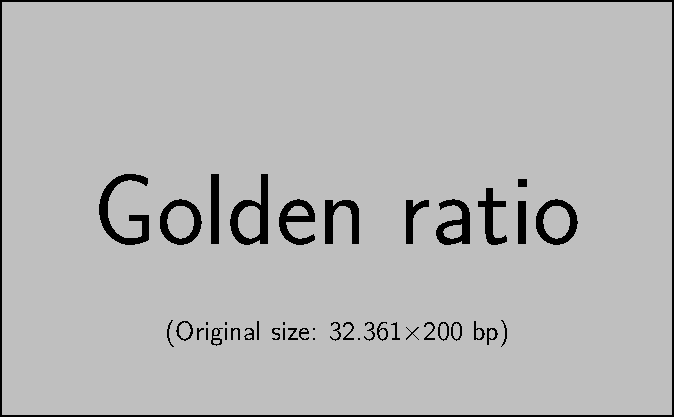
\includegraphics[width=\textwidth]{placeholder_images/example-image-golden.pdf}
    \caption[Stacking of layers within a pouch cell]
    {Image showing the stacking of layers within a pouch cell. For the negative
        electrodes, there is a small overhang (\approx\SI{2}{mm}) at the
    edges with respect to the positive electrodes. This design choice
helps to avoid plating of lithium at the edges.}
    \label{fig:anodeoverhangpouchcell}
\end{figure}

Thus,~\cref{eq:basiccapacitybalance} reduces to
\begin{equation}
    \frac{l_\text{neg}}{l_\text{pos}} = \frac{\varepsilon_\text{pos}}{\varepsilon_\text{neg}} = 1.22
\end{equation}
yielding $l_\text{neg} = \SI{72}{\micro\meter}$.

At first, it  may be surprising to  note that the values of  the particle radius
$R_\pj$ used in  both the \gls{p2d} and \gls{spm} remain  identical. However, it
is important  to note that  the \gls{p2d} equations  of the \gls{dfn}  model are
cast in  a normalised  form, \ie{}  already set  up to  account for  the overall
capacity of the  cell under consideration implicitly through usage  of a current
density  (per unit  area) for  its  simulation. Furthermore,  this explains  why
increasing the  number of  discretisation nodes does  not increase  the modelled
capacity, but  instead serves to improves  the simulation accuracy owing  to the
enhanced spatial resolution.

The  overall  active  surface  area  $A  =  n  A_\text{elec}$  is  the  combined
cross-sectional  area  of all  layers  ($n$  is  the number  of  electrochemical
(pos,sep,neg) triplets) stacked  into the pouch cell. In both  the \gls{p2d} and
\gls{spm}  models, this  parameter serves  to  scale the  external load  current
down  to  the current  density  experienced  by  each electrochemical  layer.  A
value  of  \approx\SI{30}{\ampere \per  \meter  \squared}  was reported  in  the
results section of  Subramanian~\etal{}~\cite{Subramanian2009}. When considering
a \SI{60}{\ampere\hour} pouch cell with \SI{10}{\milli\meter} exterior thickness
and  using  the  parameters  reported  in~\cite{Subramanian2009},  this  results
in  a cross-sectional  area of  \SI{2.053}{\meter\squared}\fxnote{to add:  refer
to  layer  optimisation  chapter   for  detailed  derivation}.  Considering  the
equalisation of capacity  loading, with the newly chosen thickness  value of the
negative  electrode, the  1C-rate  capacity  of the  cell  has  been revised  to
\SI{29.23}{\ampere\per\meter\squared}.

On  simulating  the \gls{p2d}  model  with  a  trickle bleeding  type  discharge
corresponding   to   a  current   of   C/500   and   logging  the   data   every
\SI{1}{\milli\second}, after reaching \SI{2.7}{\volt}\footnote{From manufacturer
datasheets  for \protect{\gls{lco}}  chemistries,  this value  is considered  to
correspond to \SI{0}{\percent} \protect{\gls{soc}}.}, the remnant concentrations
in  the two  electrodes  were noted.  The  corresponding residual  stoichiometry
values  are reported  in~\cref{tbl:lcoSimParamsSPMp2d}  and  is consistent  with
typical values reported in literature for \gls{lco} chemistries.\fxnote{citation
needed here.}  This validation is  important, since below  certain stoichiometry
thresholds, the spinel/olivine  structure of the electrodes  can become unstable
and  collapse\fxnote{citation needed?}.

Since   the   cell   behaviour   is   considered   isothermal,   the   parameter
table     in~\cref{tbl:lcoSimParamsSPMp2d}     omits     activation     energies
for    the   various    diffusivities    and    conductivities   of    materials
(see~\cref{subsec:basicspmsimsetup}  for  further thermal  considerations).  For
this  reason,~\cref{tbl:lcoSimParamsSPMp2d}  does  not  include  other  material
properties such  as specific  heats, and  thermal conductivities.  No properties
of  the  current  collectors  appear  in  the  isothermal  model  equations  for
both  the \gls{p2d}  and  \gls{spm}  models and  hence  are  omitted. All  other
electrochemical  properties,   \viz{}  stoichiometries   at  \SI{100}{\percent},
maximum concentrations, diffusivities, reaction  rate coefficients and \gls{ocp}
of  the two  electrodes remain  invariant  between the  \gls{p2d} and  \gls{spm}
models.

\subsection{Simulation Setup}\label{subsec:basicspmsimsetup}

For  reproducibility of  results, it  is important  to discuss  the system-level
parameters influencing simulation setup.

The  lower cutoff  voltage of  the cell  is chosen  to be  \SI{2.5}{\volt}. This
is  deliberately  kept  lower  than  the voltage  corresponding  to  the  cell's
\SI{0}{\percent},  \ie{}  \SI{2.7}{\volt}.  If set  above  \SI{2.7}{\volt}  even
at  infinitesimally small  discharge  currents, the  cell  would cut-off  before
achieving complete discharge. Choosing a value lower than \SI{2.7}{V} means that
the cell gets a chance to recover its terminal voltage, despite spikes in highly
dynamic  load  currents  that  might  bring the  voltage  below  this  threshold
momentarily. If a low-enough value is  not chosen, a system-level shutdown shall
be  initiated  despite possessing  the  ability  to  continue to  operate  after
recovery  of terminal  voltage.  In  this case,  choosing  a  cutoff voltage  of
\SI{2.5}{\volt}  does  not  damage  the  cell  since  checks  are  in  place  to
monitor  the \gls{soc}  and  trigger cutoff  in the  event  of charge  depletion
(see~\cref{alg:ctstimespm,alg:disctimespm}).  Northrop~\etal~\cite{Northrop2011}
use this value, although no explanation is given for the choice.

The  upper  cutoff voltage  of  the  cell  is  chosen at  \SI{4.3}{\volt}  \ie{}
\approx\SI{100}{\milli  \volt}   higher  than   the  equilibrium   \gls{ocp}  at
\SI{100}{\percent} \gls{soc}. There are several  reasons for this smaller margin
at the upper end of the voltage spectrum
\begin{description}[leftmargin=!,labelwidth=\widthof{\bfseries low
    probabilities},itemsep=1ex]

    \item[safety] li-ion  cells are less  tolerant to overcharging and  can pose
    fire hazards.

    \item[degradation]  overcharging  li-ion  cells  can  lead  to  plating  and
    accelerate other degradation mechanisms.

    \item[low  C-rates]  charging C-rates  are  typically  lower than  discharge
    C-rates.

    \item[CCCV charging]  For on-board  chargers, taper charging  (such as  in a
    \gls{cccv} profile) is activated, which  ensures that charging current drops
    off  rapidly, leading  to a  lower overvoltage  towards the  upper \gls{soc}
    range.

    \item[low probabilities] The only charging event when an electrified vehicle
    is in motion is during regenerative braking. The vehicular \gls{bms} manages
    the operating window such that the starting \gls{soc} is much lower than the
    overvoltage  that  could  be  caused due  to  braking.  Furthermore,  during
    operation, the net discharge events  occur more frequently than regenerative
    braking events.

\end{description}

For  both the  \gls{p2d} model  and the  \gls{spm} model,  the cell  temperature
is   kept   constant   at   its   initial   value   of   \SI{25}{\degreeCelsius}
(\SI{298.15}{\kelvin}). This implies that the  operation of the lithium ion cell
is assumed  to be isothermal.  While this  is not true  in general, it  is worth
noting that thermal gradients in  the through-thickness direction is negligible.
\fxnote{citation needed} Furthermore, for  the C-rates considered (<5C), typical
in a \gls{bev} application and  for short-duration transient loads studied, this
is a reasonable assumption. Detailed modelling of thermal dynamics is not within
the scope of this thesis, as the primary goal is to obtain a physics based model
incorporating  electrochemical  principles  amenable for  embedded  application.
Thus, thermal dependence of parameters through an Arrhenius-type relationship is
not  considered.    Future   work  could   include  performing   thermally  coupled
simulations, incorporating  thermally relevant  parameters and use  a simplified
heat generation expression,  \eg{} a lumped thermal model in  both the \gls{spm}
and \gls{p2d} and compare their performances.

To  understand  the parametrisation  of  initial  concentration, the  expression
for   electrolyte   conductivity   needs    to   be   examined.   As   discussed
in~\cref{subsec:spmp2dparametrisation}, the intrinsic conductivity of a specific
type  of  electrolyte  is  a  material   property  that  depends  on  the  local
concentration of \ch{Li^+} ions and  temperature. In the characterisation of the
electrolyte in Valøen and  Reimers~\cite{Valoen2005}, the polynomial expression
in~\cref{eq:kappavsCeandT} was obtained for the electrolyte conductivity.
\begin{multline}\label{eq:kappavsCeandT}
    \kappa_j(c_\text{e},T)(x,t) =  10^{-4} c_\text{e}(x,t) \bigl(-10.5 + \num{0.668e-3} c_\text{e}(x,t) + \num{0.494e-6}  c_\text{e}(x,t)^2\\
        + (0.074 - \num{1.78e-5}) c_\text{e}(x,t) - \num{8.86e-10}
    c_\text{e}(x,t)^2 \bigr)T_\text{cell}\\
	+ \left(\num{-6.96e-5} + \num{2.8e-8} c_\text{e}(x,t))T_\text{cell}^2\right)^2
\end{multline}

For  the  isothermal  case,  $T(t)  =  T_\text{cell}$.  At  equilibrium  initial
condition ($t=0$), the electrolyte concentration is uniform over the axial space $x$.
Hence,~\cref{eq:kappavsCeandT} reduces to
\begin{multline}\label{eq:kappavsCeinitandTcell}
    \kappa_j =  10^{-4} c_\text{e,0} \bigl(-10.5 + \num{0.668e-3} c_\text{e,0} + \num{0.494e-6}  c_\text{e,0}^2\\
        + (0.074 - \num{1.78e-5}) c_\text{e,0} - \num{8.86e-10}
    c_\text{e,0}^2 \bigr)T_\text{cell}\\
	+ \left(\num{-6.96e-5} + \num{2.8e-8} c_\text{e,0})T_\text{cell}^2\right)^2
\end{multline}

\begin{figure}[htbp]
    \centering
    % % This file was created by matlab2tikz.
%
\begin{tikzpicture}

\begin{axis}[%
width=2.824in,
height=3.603in,
at={(0.498in,0.486in)},
scale only axis,
point meta min=0,
point meta max=1.53340567159312,
xmin=0,
xmax=2000,
tick align=outside,
ymin=250,
ymax=350,
zmin=0,
zmax=2,
view={-37.5}{30},
axis background/.style={fill=white},
axis x line*=bottom,
axis y line*=left,
axis z line*=left,
xmajorgrids,
ymajorgrids,
zmajorgrids,
legend style={at={(1.03,1)}, anchor=north west, legend cell align=left, align=left, draw=white!15!black},
colormap={mymap}{[1pt] rgb(0pt)=(0.2422,0.1504,0.6603); rgb(1pt)=(0.25039,0.164995,0.707614); rgb(2pt)=(0.257771,0.181781,0.751138); rgb(3pt)=(0.264729,0.197757,0.795214); rgb(4pt)=(0.270648,0.214676,0.836371); rgb(5pt)=(0.275114,0.234238,0.870986); rgb(6pt)=(0.2783,0.255871,0.899071); rgb(7pt)=(0.280333,0.278233,0.9221); rgb(8pt)=(0.281338,0.300595,0.941376); rgb(9pt)=(0.281014,0.322757,0.957886); rgb(10pt)=(0.279467,0.344671,0.971676); rgb(11pt)=(0.275971,0.366681,0.982905); rgb(12pt)=(0.269914,0.3892,0.9906); rgb(13pt)=(0.260243,0.412329,0.995157); rgb(14pt)=(0.244033,0.435833,0.998833); rgb(15pt)=(0.220643,0.460257,0.997286); rgb(16pt)=(0.196333,0.484719,0.989152); rgb(17pt)=(0.183405,0.507371,0.979795); rgb(18pt)=(0.178643,0.528857,0.968157); rgb(19pt)=(0.176438,0.549905,0.952019); rgb(20pt)=(0.168743,0.570262,0.935871); rgb(21pt)=(0.154,0.5902,0.9218); rgb(22pt)=(0.146029,0.609119,0.907857); rgb(23pt)=(0.138024,0.627629,0.89729); rgb(24pt)=(0.124814,0.645929,0.888343); rgb(25pt)=(0.111252,0.6635,0.876314); rgb(26pt)=(0.0952095,0.679829,0.859781); rgb(27pt)=(0.0688714,0.694771,0.839357); rgb(28pt)=(0.0296667,0.708167,0.816333); rgb(29pt)=(0.00357143,0.720267,0.7917); rgb(30pt)=(0.00665714,0.731214,0.766014); rgb(31pt)=(0.0433286,0.741095,0.73941); rgb(32pt)=(0.0963952,0.75,0.712038); rgb(33pt)=(0.140771,0.7584,0.684157); rgb(34pt)=(0.1717,0.766962,0.655443); rgb(35pt)=(0.193767,0.775767,0.6251); rgb(36pt)=(0.216086,0.7843,0.5923); rgb(37pt)=(0.246957,0.791795,0.556743); rgb(38pt)=(0.290614,0.79729,0.518829); rgb(39pt)=(0.340643,0.8008,0.478857); rgb(40pt)=(0.3909,0.802871,0.435448); rgb(41pt)=(0.445629,0.802419,0.390919); rgb(42pt)=(0.5044,0.7993,0.348); rgb(43pt)=(0.561562,0.794233,0.304481); rgb(44pt)=(0.617395,0.787619,0.261238); rgb(45pt)=(0.671986,0.779271,0.2227); rgb(46pt)=(0.7242,0.769843,0.191029); rgb(47pt)=(0.773833,0.759805,0.16461); rgb(48pt)=(0.820314,0.749814,0.153529); rgb(49pt)=(0.863433,0.7406,0.159633); rgb(50pt)=(0.903543,0.733029,0.177414); rgb(51pt)=(0.939257,0.728786,0.209957); rgb(52pt)=(0.972757,0.729771,0.239443); rgb(53pt)=(0.995648,0.743371,0.237148); rgb(54pt)=(0.996986,0.765857,0.219943); rgb(55pt)=(0.995205,0.789252,0.202762); rgb(56pt)=(0.9892,0.813567,0.188533); rgb(57pt)=(0.978629,0.838629,0.176557); rgb(58pt)=(0.967648,0.8639,0.16429); rgb(59pt)=(0.96101,0.889019,0.153676); rgb(60pt)=(0.959671,0.913457,0.142257); rgb(61pt)=(0.962795,0.937338,0.12651); rgb(62pt)=(0.969114,0.960629,0.106362); rgb(63pt)=(0.9769,0.9839,0.0805)},
colorbar
]

\addplot3[%
surf,
shader=interp, colormap={mymap}{[1pt] rgb(0pt)=(0.2422,0.1504,0.6603); rgb(1pt)=(0.25039,0.164995,0.707614); rgb(2pt)=(0.257771,0.181781,0.751138); rgb(3pt)=(0.264729,0.197757,0.795214); rgb(4pt)=(0.270648,0.214676,0.836371); rgb(5pt)=(0.275114,0.234238,0.870986); rgb(6pt)=(0.2783,0.255871,0.899071); rgb(7pt)=(0.280333,0.278233,0.9221); rgb(8pt)=(0.281338,0.300595,0.941376); rgb(9pt)=(0.281014,0.322757,0.957886); rgb(10pt)=(0.279467,0.344671,0.971676); rgb(11pt)=(0.275971,0.366681,0.982905); rgb(12pt)=(0.269914,0.3892,0.9906); rgb(13pt)=(0.260243,0.412329,0.995157); rgb(14pt)=(0.244033,0.435833,0.998833); rgb(15pt)=(0.220643,0.460257,0.997286); rgb(16pt)=(0.196333,0.484719,0.989152); rgb(17pt)=(0.183405,0.507371,0.979795); rgb(18pt)=(0.178643,0.528857,0.968157); rgb(19pt)=(0.176438,0.549905,0.952019); rgb(20pt)=(0.168743,0.570262,0.935871); rgb(21pt)=(0.154,0.5902,0.9218); rgb(22pt)=(0.146029,0.609119,0.907857); rgb(23pt)=(0.138024,0.627629,0.89729); rgb(24pt)=(0.124814,0.645929,0.888343); rgb(25pt)=(0.111252,0.6635,0.876314); rgb(26pt)=(0.0952095,0.679829,0.859781); rgb(27pt)=(0.0688714,0.694771,0.839357); rgb(28pt)=(0.0296667,0.708167,0.816333); rgb(29pt)=(0.00357143,0.720267,0.7917); rgb(30pt)=(0.00665714,0.731214,0.766014); rgb(31pt)=(0.0433286,0.741095,0.73941); rgb(32pt)=(0.0963952,0.75,0.712038); rgb(33pt)=(0.140771,0.7584,0.684157); rgb(34pt)=(0.1717,0.766962,0.655443); rgb(35pt)=(0.193767,0.775767,0.6251); rgb(36pt)=(0.216086,0.7843,0.5923); rgb(37pt)=(0.246957,0.791795,0.556743); rgb(38pt)=(0.290614,0.79729,0.518829); rgb(39pt)=(0.340643,0.8008,0.478857); rgb(40pt)=(0.3909,0.802871,0.435448); rgb(41pt)=(0.445629,0.802419,0.390919); rgb(42pt)=(0.5044,0.7993,0.348); rgb(43pt)=(0.561562,0.794233,0.304481); rgb(44pt)=(0.617395,0.787619,0.261238); rgb(45pt)=(0.671986,0.779271,0.2227); rgb(46pt)=(0.7242,0.769843,0.191029); rgb(47pt)=(0.773833,0.759805,0.16461); rgb(48pt)=(0.820314,0.749814,0.153529); rgb(49pt)=(0.863433,0.7406,0.159633); rgb(50pt)=(0.903543,0.733029,0.177414); rgb(51pt)=(0.939257,0.728786,0.209957); rgb(52pt)=(0.972757,0.729771,0.239443); rgb(53pt)=(0.995648,0.743371,0.237148); rgb(54pt)=(0.996986,0.765857,0.219943); rgb(55pt)=(0.995205,0.789252,0.202762); rgb(56pt)=(0.9892,0.813567,0.188533); rgb(57pt)=(0.978629,0.838629,0.176557); rgb(58pt)=(0.967648,0.8639,0.16429); rgb(59pt)=(0.96101,0.889019,0.153676); rgb(60pt)=(0.959671,0.913457,0.142257); rgb(61pt)=(0.962795,0.937338,0.12651); rgb(62pt)=(0.969114,0.960629,0.106362); rgb(63pt)=(0.9769,0.9839,0.0805)}, mesh/rows=100]
table[row sep=crcr, point meta=\thisrow{c}] {%
%
x	y	z	c\\
0	258.15	0	0\\
0	258.705555555556	0	0\\
0	259.261111111111	0	0\\
0	259.816666666667	0	0\\
0	260.372222222222	0	0\\
0	260.927777777778	0	0\\
0	261.483333333333	0	0\\
0	262.038888888889	0	0\\
0	262.594444444444	0	0\\
0	263.15	0	0\\
0	263.705555555556	0	0\\
0	264.261111111111	0	0\\
0	264.816666666667	0	0\\
0	265.372222222222	0	0\\
0	265.927777777778	0	0\\
0	266.483333333333	0	0\\
0	267.038888888889	0	0\\
0	267.594444444444	0	0\\
0	268.15	0	0\\
0	268.705555555556	0	0\\
0	269.261111111111	0	0\\
0	269.816666666667	0	0\\
0	270.372222222222	0	0\\
0	270.927777777778	0	0\\
0	271.483333333333	0	0\\
0	272.038888888889	0	0\\
0	272.594444444444	0	0\\
0	273.15	0	0\\
0	273.705555555556	0	0\\
0	274.261111111111	0	0\\
0	274.816666666667	0	0\\
0	275.372222222222	0	0\\
0	275.927777777778	0	0\\
0	276.483333333333	0	0\\
0	277.038888888889	0	0\\
0	277.594444444444	0	0\\
0	278.15	0	0\\
0	278.705555555556	0	0\\
0	279.261111111111	0	0\\
0	279.816666666667	0	0\\
0	280.372222222222	0	0\\
0	280.927777777778	0	0\\
0	281.483333333333	0	0\\
0	282.038888888889	0	0\\
0	282.594444444444	0	0\\
0	283.15	0	0\\
0	283.705555555556	0	0\\
0	284.261111111111	0	0\\
0	284.816666666667	0	0\\
0	285.372222222222	0	0\\
0	285.927777777778	0	0\\
0	286.483333333333	0	0\\
0	287.038888888889	0	0\\
0	287.594444444444	0	0\\
0	288.15	0	0\\
0	288.705555555556	0	0\\
0	289.261111111111	0	0\\
0	289.816666666667	0	0\\
0	290.372222222222	0	0\\
0	290.927777777778	0	0\\
0	291.483333333333	0	0\\
0	292.038888888889	0	0\\
0	292.594444444444	0	0\\
0	293.15	0	0\\
0	293.705555555556	0	0\\
0	294.261111111111	0	0\\
0	294.816666666667	0	0\\
0	295.372222222222	0	0\\
0	295.927777777778	0	0\\
0	296.483333333333	0	0\\
0	297.038888888889	0	0\\
0	297.594444444444	0	0\\
0	298.15	0	0\\
0	298.705555555556	0	0\\
0	299.261111111111	0	0\\
0	299.816666666667	0	0\\
0	300.372222222222	0	0\\
0	300.927777777778	0	0\\
0	301.483333333333	0	0\\
0	302.038888888889	0	0\\
0	302.594444444444	0	0\\
0	303.15	0	0\\
0	303.705555555556	0	0\\
0	304.261111111111	0	0\\
0	304.816666666667	0	0\\
0	305.372222222222	0	0\\
0	305.927777777778	0	0\\
0	306.483333333333	0	0\\
0	307.038888888889	0	0\\
0	307.594444444444	0	0\\
0	308.15	0	0\\
0	308.705555555556	0	0\\
0	309.261111111111	0	0\\
0	309.816666666667	0	0\\
0	310.372222222222	0	0\\
0	310.927777777778	0	0\\
0	311.483333333333	0	0\\
0	312.038888888889	0	0\\
0	312.594444444444	0	0\\
0	313.15	0	0\\
20.2020202020202	258.15	0.0310959437699988	0.0310959437699988\\
20.2020202020202	258.705555555556	0.0314311330468054	0.0314311330468054\\
20.2020202020202	259.261111111111	0.031767436423089	0.031767436423089\\
20.2020202020202	259.816666666667	0.032104843028013	0.032104843028013\\
20.2020202020202	260.372222222222	0.0324433420127517	0.0324433420127517\\
20.2020202020202	260.927777777778	0.0327829225504909	0.0327829225504909\\
20.2020202020202	261.483333333333	0.0331235738364279	0.0331235738364279\\
20.2020202020202	262.038888888889	0.0334652850877711	0.0334652850877711\\
20.2020202020202	262.594444444444	0.0338080455437403	0.0338080455437403\\
20.2020202020202	263.15	0.0341518444655667	0.0341518444655667\\
20.2020202020202	263.705555555556	0.0344966711364929	0.0344966711364929\\
20.2020202020202	264.261111111111	0.0348425148617726	0.0348425148617726\\
20.2020202020202	264.816666666667	0.035189364968671	0.035189364968671\\
20.2020202020202	265.372222222222	0.0355372108064647	0.0355372108064647\\
20.2020202020202	265.927777777778	0.0358860417464415	0.0358860417464415\\
20.2020202020202	266.483333333333	0.0362358471819007	0.0362358471819007\\
20.2020202020202	267.038888888889	0.0365866165281527	0.0365866165281527\\
20.2020202020202	267.594444444444	0.0369383392225193	0.0369383392225193\\
20.2020202020202	268.15	0.0372910047243338	0.0372910047243338\\
20.2020202020202	268.705555555556	0.0376446025149407	0.0376446025149407\\
20.2020202020202	269.261111111111	0.037999122097696	0.037999122097696\\
20.2020202020202	269.816666666667	0.0383545529979668	0.0383545529979668\\
20.2020202020202	270.372222222222	0.0387108847631316	0.0387108847631316\\
20.2020202020202	270.927777777778	0.0390681069625803	0.0390681069625803\\
20.2020202020202	271.483333333333	0.0394262091877142	0.0394262091877142\\
20.2020202020202	272.038888888889	0.0397851810519459	0.0397851810519459\\
20.2020202020202	272.594444444444	0.0401450121906991	0.0401450121906991\\
20.2020202020202	273.15	0.0405056922614092	0.0405056922614092\\
20.2020202020202	273.705555555556	0.0408672109435227	0.0408672109435227\\
20.2020202020202	274.261111111111	0.0412295579384975	0.0412295579384975\\
20.2020202020202	274.816666666667	0.0415927229698029	0.0415927229698029\\
20.2020202020202	275.372222222222	0.0419566957829194	0.0419566957829194\\
20.2020202020202	275.927777777778	0.042321466145339	0.042321466145339\\
20.2020202020202	276.483333333333	0.0426870238465649	0.0426870238465649\\
20.2020202020202	277.038888888889	0.0430533586981117	0.0430533586981117\\
20.2020202020202	277.594444444444	0.0434204605335053	0.0434204605335053\\
20.2020202020202	278.15	0.043788319208283	0.043788319208283\\
20.2020202020202	278.705555555556	0.0441569245999934	0.0441569245999934\\
20.2020202020202	279.261111111111	0.0445262666081964	0.0445262666081964\\
20.2020202020202	279.816666666667	0.0448963351544633	0.0448963351544633\\
20.2020202020202	280.372222222222	0.0452671201823768	0.0452671201823768\\
20.2020202020202	280.927777777778	0.0456386116575306	0.0456386116575306\\
20.2020202020202	281.483333333333	0.0460107995675302	0.0460107995675302\\
20.2020202020202	282.038888888889	0.0463836739219922	0.0463836739219922\\
20.2020202020202	282.594444444444	0.0467572247525445	0.0467572247525445\\
20.2020202020202	283.15	0.0471314421128264	0.0471314421128264\\
20.2020202020202	283.705555555556	0.0475063160784885	0.0475063160784885\\
20.2020202020202	284.261111111111	0.0478818367471929	0.0478818367471929\\
20.2020202020202	284.816666666667	0.0482579942386128	0.0482579942386128\\
20.2020202020202	285.372222222222	0.0486347786944328	0.0486347786944328\\
20.2020202020202	285.927777777778	0.049012180278349	0.049012180278349\\
20.2020202020202	286.483333333333	0.0493901891760686	0.0493901891760686\\
20.2020202020202	287.038888888889	0.0497687955953104	0.0497687955953104\\
20.2020202020202	287.594444444444	0.0501479897658042	0.0501479897658042\\
20.2020202020202	288.15	0.0505277619392915	0.0505277619392915\\
20.2020202020202	288.705555555556	0.0509081023895249	0.0509081023895249\\
20.2020202020202	289.261111111111	0.0512890014122683	0.0512890014122683\\
20.2020202020202	289.816666666667	0.0516704493252971	0.0516704493252971\\
20.2020202020202	290.372222222222	0.0520524364683981	0.0520524364683981\\
20.2020202020202	290.927777777778	0.0524349532033691	0.0524349532033691\\
20.2020202020202	291.483333333333	0.0528179899140197	0.0528179899140197\\
20.2020202020202	292.038888888889	0.0532015370061704	0.0532015370061704\\
20.2020202020202	292.594444444444	0.0535855849076532	0.0535855849076532\\
20.2020202020202	293.15	0.0539701240683115	0.0539701240683115\\
20.2020202020202	293.705555555556	0.05435514496	0.05435514496\\
20.2020202020202	294.261111111111	0.0547406380765849	0.0547406380765849\\
20.2020202020202	294.816666666667	0.0551265939339433	0.0551265939339433\\
20.2020202020202	295.372222222222	0.055513003069964	0.055513003069964\\
20.2020202020202	295.927777777778	0.055899856044547	0.055899856044547\\
20.2020202020202	296.483333333333	0.0562871434396038	0.0562871434396038\\
20.2020202020202	297.038888888889	0.0566748558590572	0.0566748558590572\\
20.2020202020202	297.594444444444	0.0570629839288409	0.0570629839288409\\
20.2020202020202	298.15	0.0574515182969006	0.0574515182969006\\
20.2020202020202	298.705555555556	0.0578404496331929	0.0578404496331929\\
20.2020202020202	299.261111111111	0.0582297686296858	0.0582297686296858\\
20.2020202020202	299.816666666667	0.058619466000359	0.058619466000359\\
20.2020202020202	300.372222222222	0.0590095324812028	0.0590095324812028\\
20.2020202020202	300.927777777778	0.0593999588302196	0.0593999588302196\\
20.2020202020202	301.483333333333	0.0597907358274227	0.0597907358274227\\
20.2020202020202	302.038888888889	0.0601818542748368	0.0601818542748368\\
20.2020202020202	302.594444444444	0.0605733049964982	0.0605733049964982\\
20.2020202020202	303.15	0.060965078838454	0.060965078838454\\
20.2020202020202	303.705555555556	0.0613571666687631	0.0613571666687631\\
20.2020202020202	304.261111111111	0.0617495593774956	0.0617495593774956\\
20.2020202020202	304.816666666667	0.0621422478767331	0.0621422478767331\\
20.2020202020202	305.372222222222	0.0625352231005682	0.0625352231005682\\
20.2020202020202	305.927777777778	0.0629284760051048	0.0629284760051048\\
20.2020202020202	306.483333333333	0.0633219975684587	0.0633219975684587\\
20.2020202020202	307.038888888889	0.0637157787907566	0.0637157787907566\\
20.2020202020202	307.594444444444	0.0641098106941364	0.0641098106941364\\
20.2020202020202	308.15	0.0645040843227478	0.0645040843227478\\
20.2020202020202	308.705555555556	0.0648985907427515	0.0648985907427515\\
20.2020202020202	309.261111111111	0.0652933210423196	0.0652933210423196\\
20.2020202020202	309.816666666667	0.0656882663316356	0.0656882663316356\\
20.2020202020202	310.372222222222	0.0660834177428942	0.0660834177428942\\
20.2020202020202	310.927777777778	0.0664787664303017	0.0664787664303017\\
20.2020202020202	311.483333333333	0.0668743035700755	0.0668743035700755\\
20.2020202020202	312.038888888889	0.0672700203604444	0.0672700203604444\\
20.2020202020202	312.594444444444	0.0676659080216485	0.0676659080216485\\
20.2020202020202	313.15	0.0680619577959393	0.0680619577959393\\
40.4040404040404	258.15	0.0608889858592495	0.0608889858592495\\
40.4040404040404	258.705555555556	0.0615511269642289	0.0615511269642289\\
40.4040404040404	259.261111111111	0.0622155086688124	0.0622155086688124\\
40.4040404040404	259.816666666667	0.0628821094480045	0.0628821094480045\\
40.4040404040404	260.372222222222	0.0635509078201137	0.0635509078201137\\
40.4040404040404	260.927777777778	0.0642218823467527	0.0642218823467527\\
40.4040404040404	261.483333333333	0.0648950116328386	0.0648950116328386\\
40.4040404040404	262.038888888889	0.0655702743265928	0.0655702743265928\\
40.4040404040404	262.594444444444	0.0662476491195403	0.0662476491195403\\
40.4040404040404	263.15	0.066927114746511	0.066927114746511\\
40.4040404040404	263.705555555556	0.0676086499856386	0.0676086499856386\\
40.4040404040404	264.261111111111	0.0682922336583612	0.0682922336583612\\
40.4040404040404	264.816666666667	0.0689778446294209	0.0689778446294209\\
40.4040404040404	265.372222222222	0.0696654618068641	0.0696654618068641\\
40.4040404040404	265.927777777778	0.0703550641420413	0.0703550641420413\\
40.4040404040404	266.483333333333	0.0710466306296077	0.0710466306296077\\
40.4040404040404	267.038888888889	0.0717401403075219	0.0717401403075219\\
40.4040404040404	267.594444444444	0.0724355722570471	0.0724355722570471\\
40.4040404040404	268.15	0.0731329056027509	0.0731329056027509\\
40.4040404040404	268.705555555556	0.0738321195125049	0.0738321195125049\\
40.4040404040404	269.261111111111	0.0745331931974847	0.0745331931974847\\
40.4040404040404	269.816666666667	0.0752361059121704	0.0752361059121704\\
40.4040404040404	270.372222222222	0.0759408369543463	0.0759408369543463\\
40.4040404040404	270.927777777778	0.0766473656651006	0.0766473656651006\\
40.4040404040404	271.483333333333	0.0773556714288261	0.0773556714288261\\
40.4040404040404	272.038888888889	0.0780657336732195	0.0780657336732195\\
40.4040404040404	272.594444444444	0.0787775318692817	0.0787775318692817\\
40.4040404040404	273.15	0.0794910455313181	0.0794910455313181\\
40.4040404040404	273.705555555556	0.0802062542169379	0.0802062542169379\\
40.4040404040404	274.261111111111	0.0809231375270548	0.0809231375270548\\
40.4040404040404	274.816666666667	0.0816416751058866	0.0816416751058866\\
40.4040404040404	275.372222222222	0.0823618466409552	0.0823618466409552\\
40.4040404040404	275.927777777778	0.083083631863087	0.083083631863087\\
40.4040404040404	276.483333333333	0.0838070105464121	0.0838070105464121\\
40.4040404040404	277.038888888889	0.0845319625083652	0.0845319625083652\\
40.4040404040404	277.594444444444	0.0852584676096852	0.0852584676096852\\
40.4040404040404	278.15	0.0859865057544151	0.0859865057544151\\
40.4040404040404	278.705555555556	0.0867160568899019	0.0867160568899019\\
40.4040404040404	279.261111111111	0.0874471010067971	0.0874471010067971\\
40.4040404040404	279.816666666667	0.0881796181390563	0.0881796181390563\\
40.4040404040404	280.372222222222	0.0889135883639394	0.0889135883639394\\
40.4040404040404	280.927777777778	0.0896489918020101	0.0896489918020101\\
40.4040404040404	281.483333333333	0.0903858086171368	0.0903858086171368\\
40.4040404040404	282.038888888889	0.0911240190164919	0.0911240190164919\\
40.4040404040404	282.594444444444	0.091863603250552	0.091863603250552\\
40.4040404040404	283.15	0.0926045416130977	0.0926045416130977\\
40.4040404040404	283.705555555556	0.0933468144412141	0.0933468144412141\\
40.4040404040404	284.261111111111	0.0940904021152903	0.0940904021152903\\
40.4040404040404	284.816666666667	0.0948352850590201	0.0948352850590201\\
40.4040404040404	285.372222222222	0.0955814437394005	0.0955814437394005\\
40.4040404040404	285.927777777778	0.0963288586667336	0.0963288586667336\\
40.4040404040404	286.483333333333	0.0970775103946253	0.0970775103946253\\
40.4040404040404	287.038888888889	0.0978273795199859	0.0978273795199859\\
40.4040404040404	287.594444444444	0.0985784466830297	0.0985784466830297\\
40.4040404040404	288.15	0.0993306925672752	0.0993306925672752\\
40.4040404040404	288.705555555556	0.100084097899545	0.100084097899545\\
40.4040404040404	289.261111111111	0.100838643449967	0.100838643449967\\
40.4040404040404	289.816666666667	0.101594310031971	0.101594310031971\\
40.4040404040404	290.372222222222	0.102351078502294	0.102351078502294\\
40.4040404040404	290.927777777778	0.103108929760974	0.103108929760974\\
40.4040404040404	291.483333333333	0.103867844751356	0.103867844751356\\
40.4040404040404	292.038888888889	0.104627804460087	0.104627804460087\\
40.4040404040404	292.594444444444	0.10538878991712	0.10538878991712\\
40.4040404040404	293.15	0.10615078219571	0.10615078219571\\
40.4040404040404	293.705555555556	0.10691376241242	0.10691376241242\\
40.4040404040404	294.261111111111	0.107677711727112	0.107677711727112\\
40.4040404040404	294.816666666667	0.108442611342958	0.108442611342958\\
40.4040404040404	295.372222222222	0.109208442506428	0.109208442506428\\
40.4040404040404	295.927777777778	0.109975186507302	0.109975186507302\\
40.4040404040404	296.483333333333	0.11074282467866	0.11074282467866\\
40.4040404040404	297.038888888889	0.111511338396888	0.111511338396888\\
40.4040404040404	297.594444444444	0.112280709081677	0.112280709081677\\
40.4040404040404	298.15	0.113050918196019	0.113050918196019\\
40.4040404040404	298.705555555556	0.113821947246215	0.113821947246215\\
40.4040404040404	299.261111111111	0.114593777781866	0.114593777781866\\
40.4040404040404	299.816666666667	0.115366391395879	0.115366391395879\\
40.4040404040404	300.372222222222	0.116139769724466	0.116139769724466\\
40.4040404040404	300.927777777778	0.11691389444714	0.11691389444714\\
40.4040404040404	301.483333333333	0.117688747286723	0.117688747286723\\
40.4040404040404	302.038888888889	0.118464310009336	0.118464310009336\\
40.4040404040404	302.594444444444	0.119240564424408	0.119240564424408\\
40.4040404040404	303.15	0.120017492384672	0.120017492384672\\
40.4040404040404	303.705555555556	0.120795075786163	0.120795075786163\\
40.4040404040404	304.261111111111	0.121573296568221	0.121573296568221\\
40.4040404040404	304.816666666667	0.122352136713491	0.122352136713491\\
40.4040404040404	305.372222222222	0.123131578247922	0.123131578247922\\
40.4040404040404	305.927777777778	0.123911603240767	0.123911603240767\\
40.4040404040404	306.483333333333	0.124692193804583	0.124692193804583\\
40.4040404040404	307.038888888889	0.125473332095231	0.125473332095231\\
40.4040404040404	307.594444444444	0.126255000311877	0.126255000311877\\
40.4040404040404	308.15	0.127037180696991	0.127037180696991\\
40.4040404040404	308.705555555556	0.127819855536346	0.127819855536346\\
40.4040404040404	309.261111111111	0.128603007159022	0.128603007159022\\
40.4040404040404	309.816666666667	0.129386617937399	0.129386617937399\\
40.4040404040404	310.372222222222	0.130170670287166	0.130170670287166\\
40.4040404040404	310.927777777778	0.130955146667311	0.130955146667311\\
40.4040404040404	311.483333333333	0.131740029580132	0.131740029580132\\
40.4040404040404	312.038888888889	0.132525301571226	0.132525301571226\\
40.4040404040404	312.594444444444	0.133310945229497	0.133310945229497\\
40.4040404040404	313.15	0.134096943187153	0.134096943187153\\
60.6060606060606	258.15	0.0894098958200071	0.0894098958200071\\
60.6060606060606	258.705555555556	0.090390825677924	0.090390825677924\\
60.6060606060606	259.261111111111	0.0913751344065284	0.0913751344065284\\
60.6060606060606	259.816666666667	0.0923627900430015	0.0923627900430015\\
60.6060606060606	260.372222222222	0.0933537606884118	0.0933537606884118\\
60.6060606060606	260.927777777778	0.0943480145077156	0.0943480145077156\\
60.6060606060606	261.483333333333	0.0953455197297563	0.0953455197297563\\
60.6060606060606	262.038888888889	0.0963462446472653	0.0963462446472653\\
60.6060606060606	262.594444444444	0.0973501576168605	0.0973501576168605\\
60.6060606060606	263.15	0.0983572270590481	0.0983572270590481\\
60.6060606060606	263.705555555556	0.0993674214582215	0.0993674214582215\\
60.6060606060606	264.261111111111	0.100380709362661	0.100380709362661\\
60.6060606060606	264.816666666667	0.101397059384536	0.101397059384536\\
60.6060606060606	265.372222222222	0.102416440199902	0.102416440199902\\
60.6060606060606	265.927777777778	0.103438820548701	0.103438820548701\\
60.6060606060606	266.483333333333	0.104464169234765	0.104464169234765\\
60.6060606060606	267.038888888889	0.105492455125812	0.105492455125812\\
60.6060606060606	267.594444444444	0.106523647153447	0.106523647153447\\
60.6060606060606	268.15	0.107557714313163	0.107557714313163\\
60.6060606060606	268.705555555556	0.108594625664341	0.108594625664341\\
60.6060606060606	269.261111111111	0.109634350330248	0.109634350330248\\
60.6060606060606	269.816666666667	0.11067685749804	0.11067685749804\\
60.6060606060606	270.372222222222	0.111722116418761	0.111722116418761\\
60.6060606060606	270.927777777778	0.112770096407339	0.112770096407339\\
60.6060606060606	271.483333333333	0.113820766842593	0.113820766842593\\
60.6060606060606	272.038888888889	0.114874097167229	0.114874097167229\\
60.6060606060606	272.594444444444	0.115930056887838	0.115930056887838\\
60.6060606060606	273.15	0.116988615574901	0.116988615574901\\
60.6060606060606	273.705555555556	0.118049742862786	0.118049742862786\\
60.6060606060606	274.261111111111	0.119113408449747	0.119113408449747\\
60.6060606060606	274.816666666667	0.120179582097928	0.120179582097928\\
60.6060606060606	275.372222222222	0.121248233633357	0.121248233633357\\
60.6060606060606	275.927777777778	0.122319332945953	0.122319332945953\\
60.6060606060606	276.483333333333	0.123392849989519	0.123392849989519\\
60.6060606060606	277.038888888889	0.12446875478175	0.12446875478175\\
60.6060606060606	277.594444444444	0.125547017404223	0.125547017404223\\
60.6060606060606	278.15	0.126627608002407	0.126627608002407\\
60.6060606060606	278.705555555556	0.127710496785656	0.127710496785656\\
60.6060606060606	279.261111111111	0.128795654027213	0.128795654027213\\
60.6060606060606	279.816666666667	0.129883050064206	0.129883050064206\\
60.6060606060606	280.372222222222	0.130972655297653	0.130972655297653\\
60.6060606060606	280.927777777778	0.132064440192459	0.132064440192459\\
60.6060606060606	281.483333333333	0.133158375277415	0.133158375277415\\
60.6060606060606	282.038888888889	0.134254431145201	0.134254431145201\\
60.6060606060606	282.594444444444	0.135352578452383	0.135352578452383\\
60.6060606060606	283.15	0.136452787919416	0.136452787919416\\
60.6060606060606	283.705555555556	0.137555030330642	0.137555030330642\\
60.6060606060606	284.261111111111	0.13865927653429	0.13865927653429\\
60.6060606060606	284.816666666667	0.139765497442476	0.139765497442476\\
60.6060606060606	285.372222222222	0.140873664031205	0.140873664031205\\
60.6060606060606	285.927777777778	0.141983747340369	0.141983747340369\\
60.6060606060606	286.483333333333	0.143095718473745	0.143095718473745\\
60.6060606060606	287.038888888889	0.144209548599002	0.144209548599002\\
60.6060606060606	287.594444444444	0.145325208947692	0.145325208947692\\
60.6060606060606	288.15	0.146442670815258	0.146442670815258\\
60.6060606060606	288.705555555556	0.147561905561028	0.147561905561028\\
60.6060606060606	289.261111111111	0.148682884608218	0.148682884608218\\
60.6060606060606	289.816666666667	0.149805579443932	0.149805579443932\\
60.6060606060606	290.372222222222	0.150929961619161	0.150929961619161\\
60.6060606060606	290.927777777778	0.152056002748785	0.152056002748785\\
60.6060606060606	291.483333333333	0.153183674511569	0.153183674511569\\
60.6060606060606	292.038888888889	0.154312948650167	0.154312948650167\\
60.6060606060606	292.594444444444	0.155443796971119	0.155443796971119\\
60.6060606060606	293.15	0.156576191344855	0.156576191344855\\
60.6060606060606	293.705555555556	0.15771010370569	0.15771010370569\\
60.6060606060606	294.261111111111	0.158845506051828	0.158845506051828\\
60.6060606060606	294.816666666667	0.15998237044536	0.15998237044536\\
60.6060606060606	295.372222222222	0.161120669012263	0.161120669012263\\
60.6060606060606	295.927777777778	0.162260373942404	0.162260373942404\\
60.6060606060606	296.483333333333	0.163401457489537	0.163401457489537\\
60.6060606060606	297.038888888889	0.164543891971301	0.164543891971301\\
60.6060606060606	297.594444444444	0.165687649769224	0.165687649769224\\
60.6060606060606	298.15	0.166832703328723	0.166832703328723\\
60.6060606060606	298.705555555556	0.167979025159101	0.167979025159101\\
60.6060606060606	299.261111111111	0.169126587833547	0.169126587833547\\
60.6060606060606	299.816666666667	0.17027536398914	0.17027536398914\\
60.6060606060606	300.372222222222	0.171425326326846	0.171425326326846\\
60.6060606060606	300.927777777778	0.172576447611517	0.172576447611517\\
60.6060606060606	301.483333333333	0.173728700671893	0.173728700671893\\
60.6060606060606	302.038888888889	0.174882058400603	0.174882058400603\\
60.6060606060606	302.594444444444	0.176036493754161	0.176036493754161\\
60.6060606060606	303.15	0.177191979752971	0.177191979752971\\
60.6060606060606	303.705555555556	0.178348489481322	0.178348489481322\\
60.6060606060606	304.261111111111	0.179505996087392	0.179505996087392\\
60.6060606060606	304.816666666667	0.180664472783246	0.180664472783246\\
60.6060606060606	305.372222222222	0.181823892844837	0.181823892844837\\
60.6060606060606	305.927777777778	0.182984229612004	0.182984229612004\\
60.6060606060606	306.483333333333	0.184145456488476	0.184145456488476\\
60.6060606060606	307.038888888889	0.185307546941866	0.185307546941866\\
60.6060606060606	307.594444444444	0.186470474503678	0.186470474503678\\
60.6060606060606	308.15	0.1876342127693	0.1876342127693\\
60.6060606060606	308.705555555556	0.188798735398011	0.188798735398011\\
60.6060606060606	309.261111111111	0.189964016112975	0.189964016112975\\
60.6060606060606	309.816666666667	0.191130028701244	0.191130028701244\\
60.6060606060606	310.372222222222	0.192296747013758	0.192296747013758\\
60.6060606060606	310.927777777778	0.193464144965343	0.193464144965343\\
60.6060606060606	311.483333333333	0.194632196534715	0.194632196534715\\
60.6060606060606	312.038888888889	0.195800875764476	0.195800875764476\\
60.6060606060606	312.594444444444	0.196970156761114	0.196970156761114\\
60.6060606060606	313.15	0.198140013695006	0.198140013695006\\
80.8080808080808	258.15	0.116689011743543	0.116689011743543\\
80.8080808080808	258.705555555556	0.117980642051194	0.117980642051194\\
80.8080808080808	259.261111111111	0.119276800647025	0.119276800647025\\
80.8080808080808	259.816666666667	0.120577445346367	0.120577445346367\\
80.8080808080808	260.372222222222	0.121882534048321	0.121882534048321\\
80.8080808080808	260.927777777778	0.123192024735756	0.123192024735756\\
80.8080808080808	261.483333333333	0.124505875475314	0.124505875475314\\
80.8080808080808	262.038888888889	0.125824044417404	0.125824044417404\\
80.8080808080808	262.594444444444	0.127146489796207	0.127146489796207\\
80.8080808080808	263.15	0.128473169929674	0.128473169929674\\
80.8080808080808	263.705555555556	0.129804043219524	0.129804043219524\\
80.8080808080808	264.261111111111	0.131139068151248	0.131139068151248\\
80.8080808080808	264.816666666667	0.132478203294107	0.132478203294107\\
80.8080808080808	265.372222222222	0.133821407301131	0.133821407301131\\
80.8080808080808	265.927777777778	0.135168638909119	0.135168638909119\\
80.8080808080808	266.483333333333	0.136519856938642	0.136519856938642\\
80.8080808080808	267.038888888889	0.13787502029404	0.13787502029404\\
80.8080808080808	267.594444444444	0.139234087963424	0.139234087963424\\
80.8080808080808	268.15	0.140597019018673	0.140597019018673\\
80.8080808080808	268.705555555556	0.141963772615437	0.141963772615437\\
80.8080808080808	269.261111111111	0.143334307993137	0.143334307993137\\
80.8080808080808	269.816666666667	0.144708584474963	0.144708584474963\\
80.8080808080808	270.372222222222	0.146086561467874	0.146086561467874\\
80.8080808080808	270.927777777778	0.1474681984626	0.1474681984626\\
80.8080808080808	271.483333333333	0.148853455033642	0.148853455033642\\
80.8080808080808	272.038888888889	0.150242290839269	0.150242290839269\\
80.8080808080808	272.594444444444	0.151634665621521	0.151634665621521\\
80.8080808080808	273.15	0.153030539206208	0.153030539206208\\
80.8080808080808	273.705555555556	0.154429871502909	0.154429871502909\\
80.8080808080808	274.261111111111	0.155832622504975	0.155832622504975\\
80.8080808080808	274.816666666667	0.157238752289526	0.157238752289526\\
80.8080808080808	275.372222222222	0.158648221017451	0.158648221017451\\
80.8080808080808	275.927777777778	0.160060988933409	0.160060988933409\\
80.8080808080808	276.483333333333	0.16147701636583	0.16147701636583\\
80.8080808080808	277.038888888889	0.162896263726914	0.162896263726914\\
80.8080808080808	277.594444444444	0.164318691512632	0.164318691512632\\
80.8080808080808	278.15	0.165744260302721	0.165744260302721\\
80.8080808080808	278.705555555556	0.167172930760691	0.167172930760691\\
80.8080808080808	279.261111111111	0.168604663633823	0.168604663633823\\
80.8080808080808	279.816666666667	0.170039419753166	0.170039419753166\\
80.8080808080808	280.372222222222	0.171477160033538	0.171477160033538\\
80.8080808080808	280.927777777778	0.17291784547353	0.17291784547353\\
80.8080808080808	281.483333333333	0.174361437155501	0.174361437155501\\
80.8080808080808	282.038888888889	0.17580789624558	0.17580789624558\\
80.8080808080808	282.594444444444	0.177257183993667	0.177257183993667\\
80.8080808080808	283.15	0.178709261733431	0.178709261733431\\
80.8080808080808	283.705555555556	0.18016409088231	0.18016409088231\\
80.8080808080808	284.261111111111	0.181621632941515	0.181621632941515\\
80.8080808080808	284.816666666667	0.183081849496025	0.183081849496025\\
80.8080808080808	285.372222222222	0.184544702214589	0.184544702214589\\
80.8080808080808	285.927777777778	0.186010152849725	0.186010152849725\\
80.8080808080808	286.483333333333	0.187478163237724	0.187478163237724\\
80.8080808080808	287.038888888889	0.188948695298644	0.188948695298644\\
80.8080808080808	287.594444444444	0.190421711036314	0.190421711036314\\
80.8080808080808	288.15	0.191897172538333	0.191897172538333\\
80.8080808080808	288.705555555556	0.19337504197607	0.19337504197607\\
80.8080808080808	289.261111111111	0.194855281604665	0.194855281604665\\
80.8080808080808	289.816666666667	0.196337853763026	0.196337853763026\\
80.8080808080808	290.372222222222	0.197822720873832	0.197822720873832\\
80.8080808080808	290.927777777778	0.199309845443531	0.199309845443531\\
80.8080808080808	291.483333333333	0.200799190062344	0.200799190062344\\
80.8080808080808	292.038888888889	0.202290717404259	0.202290717404259\\
80.8080808080808	292.594444444444	0.203784390227034	0.203784390227034\\
80.8080808080808	293.15	0.205280171372198	0.205280171372198\\
80.8080808080808	293.705555555556	0.20677802376505	0.20677802376505\\
80.8080808080808	294.261111111111	0.208277910414659	0.208277910414659\\
80.8080808080808	294.816666666667	0.209779794413863	0.209779794413863\\
80.8080808080808	295.372222222222	0.211283638939271	0.211283638939271\\
80.8080808080808	295.927777777778	0.212789407251262	0.212789407251262\\
80.8080808080808	296.483333333333	0.214297062693984	0.214297062693984\\
80.8080808080808	297.038888888889	0.215806568695356	0.215806568695356\\
80.8080808080808	297.594444444444	0.217317888767066	0.217317888767066\\
80.8080808080808	298.15	0.218830986504573	0.218830986504573\\
80.8080808080808	298.705555555556	0.220345825587105	0.220345825587105\\
80.8080808080808	299.261111111111	0.221862369777661	0.221862369777661\\
80.8080808080808	299.816666666667	0.223380582923009	0.223380582923009\\
80.8080808080808	300.372222222222	0.224900428953688	0.224900428953688\\
80.8080808080808	300.927777777778	0.226421871884005	0.226421871884005\\
80.8080808080808	301.483333333333	0.22794487581204	0.22794487581204\\
80.8080808080808	302.038888888889	0.229469404919641	0.229469404919641\\
80.8080808080808	302.594444444444	0.230995423472424	0.230995423472424\\
80.8080808080808	303.15	0.232522895819781	0.232522895819781\\
80.8080808080808	303.705555555556	0.234051786394867	0.234051786394867\\
80.8080808080808	304.261111111111	0.235582059714611	0.235582059714611\\
80.8080808080808	304.816666666667	0.237113680379713	0.237113680379713\\
80.8080808080808	305.372222222222	0.238646613074638	0.238646613074638\\
80.8080808080808	305.927777777778	0.240180822567627	0.240180822567627\\
80.8080808080808	306.483333333333	0.241716273710687	0.241716273710687\\
80.8080808080808	307.038888888889	0.243252931439595	0.243252931439595\\
80.8080808080808	307.594444444444	0.2447907607739	0.2447907607739\\
80.8080808080808	308.15	0.24632972681692	0.24632972681692\\
80.8080808080808	308.705555555556	0.247869794755743	0.247869794755743\\
80.8080808080808	309.261111111111	0.249410929861226	0.249410929861226\\
80.8080808080808	309.816666666667	0.250953097487997	0.250953097487997\\
80.8080808080808	310.372222222222	0.252496263074456	0.252496263074456\\
80.8080808080808	310.927777777778	0.254040392142768	0.254040392142768\\
80.8080808080808	311.483333333333	0.255585450298873	0.255585450298873\\
80.8080808080808	312.038888888889	0.257131403232477	0.257131403232477\\
80.8080808080808	312.594444444444	0.258678216717059	0.258678216717059\\
80.8080808080808	313.15	0.260225856609865	0.260225856609865\\
101.010101010101	258.15	0.142756243101733	0.142756243101733\\
101.010101010101	258.705555555556	0.144350560716045	0.144350560716045\\
101.010101010101	259.261111111111	0.14595056656306	0.14595056656306\\
101.010101010101	259.816666666667	0.147556208451845	0.147556208451845\\
101.010101010101	260.372222222222	0.14916743429443	0.14916743429443\\
101.010101010101	260.927777777778	0.150784192105806	0.150784192105806\\
101.010101010101	261.483333333333	0.152406430003923	0.152406430003923\\
101.010101010101	262.038888888889	0.154034096209693	0.154034096209693\\
101.010101010101	262.594444444444	0.155667139046988	0.155667139046988\\
101.010101010101	263.15	0.157305506942642	0.157305506942642\\
101.010101010101	263.705555555556	0.158949148426446	0.158949148426446\\
101.010101010101	264.261111111111	0.160598012131155	0.160598012131155\\
101.010101010101	264.816666666667	0.162252046792485	0.162252046792485\\
101.010101010101	265.372222222222	0.163911201249108	0.163911201249108\\
101.010101010101	265.927777777778	0.165575424442663	0.165575424442663\\
101.010101010101	266.483333333333	0.167244665417744	0.167244665417744\\
101.010101010101	267.038888888889	0.168918873321911	0.168918873321911\\
101.010101010101	267.594444444444	0.170597997405678	0.170597997405678\\
101.010101010101	268.15	0.172281987022525	0.172281987022525\\
101.010101010101	268.705555555556	0.173970791628892	0.173970791628892\\
101.010101010101	269.261111111111	0.175664360784176	0.175664360784176\\
101.010101010101	269.816666666667	0.177362644150739	0.177362644150739\\
101.010101010101	270.372222222222	0.179065591493901	0.179065591493901\\
101.010101010101	270.927777777778	0.180773152681943	0.180773152681943\\
101.010101010101	271.483333333333	0.182485277686108	0.182485277686108\\
101.010101010101	272.038888888889	0.184201916580598	0.184201916580598\\
101.010101010101	272.594444444444	0.185923019542575	0.185923019542575\\
101.010101010101	273.15	0.187648536852164	0.187648536852164\\
101.010101010101	273.705555555556	0.189378418892449	0.189378418892449\\
101.010101010101	274.261111111111	0.191112616149475	0.191112616149475\\
101.010101010101	274.816666666667	0.192851079212248	0.192851079212248\\
101.010101010101	275.372222222222	0.194593758772733	0.194593758772733\\
101.010101010101	275.927777777778	0.196340605625859	0.196340605625859\\
101.010101010101	276.483333333333	0.198091570669511	0.198091570669511\\
101.010101010101	277.038888888889	0.199846604904538	0.199846604904538\\
101.010101010101	277.594444444444	0.201605659434749	0.201605659434749\\
101.010101010101	278.15	0.203368685466913	0.203368685466913\\
101.010101010101	278.705555555556	0.20513563431076	0.20513563431076\\
101.010101010101	279.261111111111	0.206906457378981	0.206906457378981\\
101.010101010101	279.816666666667	0.208681106187226	0.208681106187226\\
101.010101010101	280.372222222222	0.210459532354107	0.210459532354107\\
101.010101010101	280.927777777778	0.212241687601197	0.212241687601197\\
101.010101010101	281.483333333333	0.214027523753028	0.214027523753028\\
101.010101010101	282.038888888889	0.215816992737094	0.215816992737094\\
101.010101010101	282.594444444444	0.21761004658385	0.21761004658385\\
101.010101010101	283.15	0.219406637426709	0.219406637426709\\
101.010101010101	283.705555555556	0.221206717502047	0.221206717502047\\
101.010101010101	284.261111111111	0.223010239149201	0.223010239149201\\
101.010101010101	284.816666666667	0.224817154810468	0.224817154810468\\
101.010101010101	285.372222222222	0.226627417031103	0.226627417031103\\
101.010101010101	285.927777777778	0.228440978459325	0.228440978459325\\
101.010101010101	286.483333333333	0.230257791846313	0.230257791846313\\
101.010101010101	287.038888888889	0.232077810046205	0.232077810046205\\
101.010101010101	287.594444444444	0.233900986016102	0.233900986016102\\
101.010101010101	288.15	0.235727272816063	0.235727272816063\\
101.010101010101	288.705555555556	0.237556623609109	0.237556623609109\\
101.010101010101	289.261111111111	0.239388991661223	0.239388991661223\\
101.010101010101	289.816666666667	0.241224330341345	0.241224330341345\\
101.010101010101	290.372222222222	0.243062593121379	0.243062593121379\\
101.010101010101	290.927777777778	0.244903733576188	0.244903733576188\\
101.010101010101	291.483333333333	0.246747705383597	0.246747705383597\\
101.010101010101	292.038888888889	0.248594462324389	0.248594462324389\\
101.010101010101	292.594444444444	0.25044395828231	0.25044395828231\\
101.010101010101	293.15	0.252296147244066	0.252296147244066\\
101.010101010101	293.705555555556	0.254150983299323	0.254150983299323\\
101.010101010101	294.261111111111	0.256008420640707	0.256008420640707\\
101.010101010101	294.816666666667	0.257868413563808	0.257868413563808\\
101.010101010101	295.372222222222	0.259730916467172	0.259730916467172\\
101.010101010101	295.927777777778	0.26159588385231	0.26159588385231\\
101.010101010101	296.483333333333	0.263463270323689	0.263463270323689\\
101.010101010101	297.038888888889	0.265333030588741	0.265333030588741\\
101.010101010101	297.594444444444	0.267205119457856	0.267205119457856\\
101.010101010101	298.15	0.269079491844386	0.269079491844386\\
101.010101010101	298.705555555556	0.270956102764642	0.270956102764642\\
101.010101010101	299.261111111111	0.272834907337897	0.272834907337897\\
101.010101010101	299.816666666667	0.274715860786384	0.274715860786384\\
101.010101010101	300.372222222222	0.276598918435296	0.276598918435296\\
101.010101010101	300.927777777778	0.278484035712789	0.278484035712789\\
101.010101010101	301.483333333333	0.280371168149977	0.280371168149977\\
101.010101010101	302.038888888889	0.282260271380936	0.282260271380936\\
101.010101010101	302.594444444444	0.284151301142701	0.284151301142701\\
101.010101010101	303.15	0.286044213275271	0.286044213275271\\
101.010101010101	303.705555555556	0.287938963721601	0.287938963721601\\
101.010101010101	304.261111111111	0.289835508527611	0.289835508527611\\
101.010101010101	304.816666666667	0.291733803842179	0.291733803842179\\
101.010101010101	305.372222222222	0.293633805917143	0.293633805917143\\
101.010101010101	305.927777777778	0.295535471107305	0.295535471107305\\
101.010101010101	306.483333333333	0.297438755870425	0.297438755870425\\
101.010101010101	307.038888888889	0.299343616767223	0.299343616767223\\
101.010101010101	307.594444444444	0.301250010461382	0.301250010461382\\
101.010101010101	308.15	0.303157893719543	0.303157893719543\\
101.010101010101	308.705555555556	0.30506722341131	0.30506722341131\\
101.010101010101	309.261111111111	0.306977956509246	0.306977956509246\\
101.010101010101	309.816666666667	0.308890050088876	0.308890050088876\\
101.010101010101	310.372222222222	0.310803461328683	0.310803461328683\\
101.010101010101	310.927777777778	0.312718147510114	0.312718147510114\\
101.010101010101	311.483333333333	0.314634066017576	0.314634066017576\\
101.010101010101	312.038888888889	0.316551174338433	0.316551174338433\\
101.010101010101	312.594444444444	0.318469430063013	0.318469430063013\\
101.010101010101	313.15	0.320388790884605	0.320388790884605\\
121.212121212121	258.15	0.16764107358865	0.16764107358865\\
121.212121212121	258.705555555556	0.169530140904245	0.169530140904245\\
121.212121212121	259.261111111111	0.171426066309897	0.171426066309897\\
121.212121212121	259.816666666667	0.173328787823598	0.173328787823598\\
121.212121212121	260.372222222222	0.175238243584809	0.175238243584809\\
121.212121212121	260.927777777778	0.17715437185446	0.17715437185446\\
121.212121212121	261.483333333333	0.179077111014948	0.179077111014948\\
121.212121212121	262.038888888889	0.18100639957014	0.18100639957014\\
121.212121212121	262.594444444444	0.18294217614537	0.18294217614537\\
121.212121212121	263.15	0.18488437948744	0.18488437948744\\
121.212121212121	263.705555555556	0.18683294846462	0.18683294846462\\
121.212121212121	264.261111111111	0.18878782206665	0.18878782206665\\
121.212121212121	264.816666666667	0.190748939404737	0.190748939404737\\
121.212121212121	265.372222222222	0.192716239711556	0.192716239711556\\
121.212121212121	265.927777777778	0.194689662341251	0.194689662341251\\
121.212121212121	266.483333333333	0.196669146769434	0.196669146769434\\
121.212121212121	267.038888888889	0.198654632593185	0.198654632593185\\
121.212121212121	267.594444444444	0.200646059531053	0.200646059531053\\
121.212121212121	268.15	0.202643367423053	0.202643367423053\\
121.212121212121	268.705555555556	0.204646496230672	0.204646496230672\\
121.212121212121	269.261111111111	0.206655386036862	0.206655386036862\\
121.212121212121	269.816666666667	0.208669977046044	0.208669977046044\\
121.212121212121	270.372222222222	0.210690209584109	0.210690209584109\\
121.212121212121	270.927777777778	0.212716024098413	0.212716024098413\\
121.212121212121	271.483333333333	0.214747361157784	0.214747361157784\\
121.212121212121	272.038888888889	0.216784161452516	0.216784161452516\\
121.212121212121	272.594444444444	0.218826365794371	0.218826365794371\\
121.212121212121	273.15	0.220873915116581	0.220873915116581\\
121.212121212121	273.705555555556	0.222926750473843	0.222926750473843\\
121.212121212121	274.261111111111	0.224984813042327	0.224984813042327\\
121.212121212121	274.816666666667	0.227048044119667	0.227048044119667\\
121.212121212121	275.372222222222	0.229116385124967	0.229116385124967\\
121.212121212121	275.927777777778	0.2311897775988	0.2311897775988\\
121.212121212121	276.483333333333	0.233268163203206	0.233268163203206\\
121.212121212121	277.038888888889	0.235351483721692	0.235351483721692\\
121.212121212121	277.594444444444	0.237439681059238	0.237439681059238\\
121.212121212121	278.15	0.239532697242287	0.239532697242287\\
121.212121212121	278.705555555556	0.241630474418752	0.241630474418752\\
121.212121212121	279.261111111111	0.243732954858016	0.243732954858016\\
121.212121212121	279.816666666667	0.245840080950929	0.245840080950929\\
121.212121212121	280.372222222222	0.247951795209808	0.247951795209808\\
121.212121212121	280.927777777778	0.250068040268439	0.250068040268439\\
121.212121212121	281.483333333333	0.252188758882078	0.252188758882078\\
121.212121212121	282.038888888889	0.254313893927448	0.254313893927448\\
121.212121212121	282.594444444444	0.256443388402739	0.256443388402739\\
121.212121212121	283.15	0.25857718542761	0.25857718542761\\
121.212121212121	283.705555555556	0.26071522824319	0.26071522824319\\
121.212121212121	284.261111111111	0.262857460212074	0.262857460212074\\
121.212121212121	284.816666666667	0.265003824818326	0.265003824818326\\
121.212121212121	285.372222222222	0.26715426566748	0.26715426566748\\
121.212121212121	285.927777777778	0.269308726486534	0.269308726486534\\
121.212121212121	286.483333333333	0.271467151123958	0.271467151123958\\
121.212121212121	287.038888888889	0.27362948354969	0.27362948354969\\
121.212121212121	287.594444444444	0.275795667855134	0.275795667855134\\
121.212121212121	288.15	0.277965648253164	0.277965648253164\\
121.212121212121	288.705555555556	0.280139369078123	0.280139369078123\\
121.212121212121	289.261111111111	0.282316774785819	0.282316774785819\\
121.212121212121	289.816666666667	0.284497809953532	0.284497809953532\\
121.212121212121	290.372222222222	0.286682419280008	0.286682419280008\\
121.212121212121	290.927777777778	0.288870547585461	0.288870547585461\\
121.212121212121	291.483333333333	0.291062139811576	0.291062139811576\\
121.212121212121	292.038888888889	0.293257141021502	0.293257141021502\\
121.212121212121	292.594444444444	0.295455496399861	0.295455496399861\\
121.212121212121	293.15	0.297657151252739	0.297657151252739\\
121.212121212121	293.705555555556	0.299862051007693	0.299862051007693\\
121.212121212121	294.261111111111	0.302070141213746	0.302070141213746\\
121.212121212121	294.816666666667	0.304281367541393	0.304281367541393\\
121.212121212121	295.372222222222	0.306495675782592	0.306495675782592\\
121.212121212121	295.927777777778	0.308713011850774	0.308713011850774\\
121.212121212121	296.483333333333	0.310933321780836	0.310933321780836\\
121.212121212121	297.038888888889	0.313156551729143	0.313156551729143\\
121.212121212121	297.594444444444	0.315382647973529	0.315382647973529\\
121.212121212121	298.15	0.317611556913297	0.317611556913297\\
121.212121212121	298.705555555556	0.319843225069216	0.319843225069216\\
121.212121212121	299.261111111111	0.322077599083524	0.322077599083524\\
121.212121212121	299.816666666667	0.32431462571993	0.32431462571993\\
121.212121212121	300.372222222222	0.326554251863607	0.326554251863607\\
121.212121212121	300.927777777778	0.3287964245212	0.3287964245212\\
121.212121212121	301.483333333333	0.331041090820819	0.331041090820819\\
121.212121212121	302.038888888889	0.333288198012045	0.333288198012045\\
121.212121212121	302.594444444444	0.335537693465925	0.335537693465925\\
121.212121212121	303.15	0.337789524674976	0.337789524674976\\
121.212121212121	303.705555555556	0.340043639253182	0.340043639253182\\
121.212121212121	304.261111111111	0.342299984935996	0.342299984935996\\
121.212121212121	304.816666666667	0.34455850958034	0.34455850958034\\
121.212121212121	305.372222222222	0.346819161164601	0.346819161164601\\
121.212121212121	305.927777777778	0.349081887788639	0.349081887788639\\
121.212121212121	306.483333333333	0.351346637673778	0.351346637673778\\
121.212121212121	307.038888888889	0.353613359162814	0.353613359162814\\
121.212121212121	307.594444444444	0.355882000720007	0.355882000720007\\
121.212121212121	308.15	0.358152510931088	0.358152510931088\\
121.212121212121	308.705555555556	0.360424838503257	0.360424838503257\\
121.212121212121	309.261111111111	0.36269893226518	0.36269893226518\\
121.212121212121	309.816666666667	0.364974741166993	0.364974741166993\\
121.212121212121	310.372222222222	0.367252214280299	0.367252214280299\\
121.212121212121	310.927777777778	0.369531300798169	0.369531300798169\\
121.212121212121	311.483333333333	0.371811950035144	0.371811950035144\\
121.212121212121	312.038888888889	0.374094111427233	0.374094111427233\\
121.212121212121	312.594444444444	0.37637773453191	0.37637773453191\\
121.212121212121	313.15	0.378662769028123	0.378662769028123\\
141.414141414141	258.15	0.19137256396215	0.19137256396215\\
141.414141414141	258.705555555556	0.193548519278371	0.193548519278371\\
141.414141414141	259.261111111111	0.195732511845846	0.195732511845846\\
141.414141414141	259.816666666667	0.197924470106253	0.197924470106253\\
141.414141414141	260.372222222222	0.200124322640573	0.200124322640573\\
141.414141414141	260.927777777778	0.202331998169086	0.202331998169086\\
141.414141414141	261.483333333333	0.204547425551375	0.204547425551375\\
141.414141414141	262.038888888889	0.206770533786327	0.206770533786327\\
141.414141414141	262.594444444444	0.209001252012128	0.209001252012128\\
141.414141414141	263.15	0.211239509506264	0.211239509506264\\
141.414141414141	263.705555555556	0.213485235685529	0.213485235685529\\
141.414141414141	264.261111111111	0.215738360106012	0.215738360106012\\
141.414141414141	264.816666666667	0.217998812463108	0.217998812463108\\
141.414141414141	265.372222222222	0.220266522591513	0.220266522591513\\
141.414141414141	265.927777777778	0.222541420465223	0.222541420465223\\
141.414141414141	266.483333333333	0.224823436197538	0.224823436197538\\
141.414141414141	267.038888888889	0.227112500041058	0.227112500041058\\
141.414141414141	267.594444444444	0.229408542387685	0.229408542387685\\
141.414141414141	268.15	0.231711493768624	0.231711493768624\\
141.414141414141	268.705555555556	0.234021284854381	0.234021284854381\\
141.414141414141	269.261111111111	0.236337846454763	0.236337846454763\\
141.414141414141	269.816666666667	0.238661109518879	0.238661109518879\\
141.414141414141	270.372222222222	0.240991005135142	0.240991005135142\\
141.414141414141	270.927777777778	0.243327464531264	0.243327464531264\\
141.414141414141	271.483333333333	0.245670419074258	0.245670419074258\\
141.414141414141	272.038888888889	0.248019800270443	0.248019800270443\\
141.414141414141	272.594444444444	0.250375539765435	0.250375539765435\\
141.414141414141	273.15	0.252737569344155	0.252737569344155\\
141.414141414141	273.705555555556	0.255105820930825	0.255105820930825\\
141.414141414141	274.261111111111	0.257480226588967	0.257480226588967\\
141.414141414141	274.816666666667	0.259860718521408	0.259860718521408\\
141.414141414141	275.372222222222	0.262247229070273	0.262247229070273\\
141.414141414141	275.927777777778	0.26463969071699	0.26463969071699\\
141.414141414141	276.483333333333	0.267038036082292	0.267038036082292\\
141.414141414141	277.038888888889	0.26944219792621	0.26944219792621\\
141.414141414141	277.594444444444	0.271852109148077	0.271852109148077\\
141.414141414141	278.15	0.274267702786529	0.274267702786529\\
141.414141414141	278.705555555556	0.276688912019503	0.276688912019503\\
141.414141414141	279.261111111111	0.279115670164238	0.279115670164238\\
141.414141414141	279.816666666667	0.281547910677277	0.281547910677277\\
141.414141414141	280.372222222222	0.28398556715446	0.28398556715446\\
141.414141414141	280.927777777778	0.286428573330931	0.286428573330931\\
141.414141414141	281.483333333333	0.288876863081138	0.288876863081138\\
141.414141414141	282.038888888889	0.291330370418828	0.291330370418828\\
141.414141414141	282.594444444444	0.29378902949705	0.29378902949705\\
141.414141414141	283.15	0.296252774608155	0.296252774608155\\
141.414141414141	283.705555555556	0.298721540183798	0.298721540183798\\
141.414141414141	284.261111111111	0.301195260794931	0.301195260794931\\
141.414141414141	284.816666666667	0.303673871151813	0.303673871151813\\
141.414141414141	285.372222222222	0.306157306104001	0.306157306104001\\
141.414141414141	285.927777777778	0.308645500640354	0.308645500640354\\
141.414141414141	286.483333333333	0.311138389889035	0.311138389889035\\
141.414141414141	287.038888888889	0.313635909117508	0.313635909117508\\
141.414141414141	287.594444444444	0.316137993732537	0.316137993732537\\
141.414141414141	288.15	0.31864457928019	0.31864457928019\\
141.414141414141	288.705555555556	0.321155601445835	0.321155601445835\\
141.414141414141	289.261111111111	0.323670996054142	0.323670996054142\\
141.414141414141	289.816666666667	0.326190699069084	0.326190699069084\\
141.414141414141	290.372222222222	0.328714646593935	0.328714646593935\\
141.414141414141	290.927777777778	0.33124277487127	0.33124277487127\\
141.414141414141	291.483333333333	0.333775020282967	0.333775020282967\\
141.414141414141	292.038888888889	0.336311319350205	0.336311319350205\\
141.414141414141	292.594444444444	0.338851608733465	0.338851608733465\\
141.414141414141	293.15	0.341395825232529	0.341395825232529\\
141.414141414141	293.705555555556	0.343943905786482	0.343943905786482\\
141.414141414141	294.261111111111	0.346495787473711	0.346495787473711\\
141.414141414141	294.816666666667	0.349051407511902	0.349051407511902\\
141.414141414141	295.372222222222	0.351610703258046	0.351610703258046\\
141.414141414141	295.927777777778	0.354173612208434	0.354173612208434\\
141.414141414141	296.483333333333	0.356740071998658	0.356740071998658\\
141.414141414141	297.038888888889	0.359310020403615	0.359310020403615\\
141.414141414141	297.594444444444	0.3618833953375	0.3618833953375\\
141.414141414141	298.15	0.364460134853812	0.364460134853812\\
141.414141414141	298.705555555556	0.367040177145351	0.367040177145351\\
141.414141414141	299.261111111111	0.369623460544219	0.369623460544219\\
141.414141414141	299.816666666667	0.372209923521819	0.372209923521819\\
141.414141414141	300.372222222222	0.374799504688857	0.374799504688857\\
141.414141414141	300.927777777778	0.37739214279534	0.37739214279534\\
141.414141414141	301.483333333333	0.379987776730576	0.379987776730576\\
141.414141414141	302.038888888889	0.382586345523176	0.382586345523176\\
141.414141414141	302.594444444444	0.385187788341053	0.385187788341053\\
141.414141414141	303.15	0.38779204449142	0.38779204449142\\
141.414141414141	303.705555555556	0.390399053420793	0.390399053420793\\
141.414141414141	304.261111111111	0.393008754714991	0.393008754714991\\
141.414141414141	304.816666666667	0.395621088099131	0.395621088099131\\
141.414141414141	305.372222222222	0.398235993437636	0.398235993437636\\
141.414141414141	305.927777777778	0.400853410734227	0.400853410734227\\
141.414141414141	306.483333333333	0.40347328013193	0.40347328013193\\
141.414141414141	307.038888888889	0.40609554191307	0.40609554191307\\
141.414141414141	307.594444444444	0.408720136499276	0.408720136499276\\
141.414141414141	308.15	0.411347004451477	0.411347004451477\\
141.414141414141	308.705555555556	0.413976086469905	0.413976086469905\\
141.414141414141	309.261111111111	0.416607323394093	0.416607323394093\\
141.414141414141	309.816666666667	0.419240656202877	0.419240656202877\\
141.414141414141	310.372222222222	0.421876026014391	0.421876026014391\\
141.414141414141	310.927777777778	0.424513374086076	0.424513374086076\\
141.414141414141	311.483333333333	0.427152641814672	0.427152641814672\\
141.414141414141	312.038888888889	0.429793770736219	0.429793770736219\\
141.414141414141	312.594444444444	0.432436702526063	0.432436702526063\\
141.414141414141	313.15	0.435081378998849	0.435081378998849\\
161.616161616162	258.15	0.213979354885464	0.213979354885464\\
161.616161616162	258.705555555556	0.216434412762867	0.216434412762867\\
161.616161616162	259.261111111111	0.218898695752802	0.218898695752802\\
161.616161616162	259.816666666667	0.221372122934946	0.221372122934946\\
161.616161616162	260.372222222222	0.22385461354545	0.22385461354545\\
161.616161616162	260.927777777778	0.226346086976933	0.226346086976933\\
161.616161616162	261.483333333333	0.228846462778486	0.228846462778486\\
161.616161616162	262.038888888889	0.231355660655667	0.231355660655667\\
161.616161616162	262.594444444444	0.233873600470505	0.233873600470505\\
161.616161616162	263.15	0.236400202241501	0.236400202241501\\
161.616161616162	263.705555555556	0.238935386143623	0.238935386143623\\
161.616161616162	264.261111111111	0.241479072508313	0.241479072508313\\
161.616161616162	264.816666666667	0.244031181823477	0.244031181823477\\
161.616161616162	265.372222222222	0.246591634733497	0.246591634733497\\
161.616161616162	265.927777777778	0.24916035203922	0.24916035203922\\
161.616161616162	266.483333333333	0.251737254697967	0.251737254697967\\
161.616161616162	267.038888888889	0.254322263823527	0.254322263823527\\
161.616161616162	267.594444444444	0.256915300686158	0.256915300686158\\
161.616161616162	268.15	0.259516286712591	0.259516286712591\\
161.616161616162	268.705555555556	0.262125143486024	0.262125143486024\\
161.616161616162	269.261111111111	0.264741792746126	0.264741792746126\\
161.616161616162	269.816666666667	0.267366156389037	0.267366156389037\\
161.616161616162	270.372222222222	0.269998156467364	0.269998156467364\\
161.616161616162	270.927777777778	0.272637715190189	0.272637715190189\\
161.616161616162	271.483333333333	0.275284754923058	0.275284754923058\\
161.616161616162	272.038888888889	0.277939198187992	0.277939198187992\\
161.616161616162	272.594444444444	0.280600967663479	0.280600967663479\\
161.616161616162	273.15	0.283269986184478	0.283269986184478\\
161.616161616162	273.705555555556	0.285946176742418	0.285946176742418\\
161.616161616162	274.261111111111	0.288629462485198	0.288629462485198\\
161.616161616162	274.816666666667	0.291319766717187	0.291319766717187\\
161.616161616162	275.372222222222	0.294017012899223	0.294017012899223\\
161.616161616162	275.927777777778	0.296721124648614	0.296721124648614\\
161.616161616162	276.483333333333	0.29943202573914	0.29943202573914\\
161.616161616162	277.038888888889	0.30214964010105	0.30214964010105\\
161.616161616162	277.594444444444	0.304873891821061	0.304873891821061\\
161.616161616162	278.15	0.307604705142363	0.307604705142363\\
161.616161616162	278.705555555556	0.310342004464614	0.310342004464614\\
161.616161616162	279.261111111111	0.313085714343943	0.313085714343943\\
161.616161616162	279.816666666667	0.315835759492947	0.315835759492947\\
161.616161616162	280.372222222222	0.318592064780697	0.318592064780697\\
161.616161616162	280.927777777778	0.321354555232728	0.321354555232728\\
161.616161616162	281.483333333333	0.324123156031052	0.324123156031052\\
161.616161616162	282.038888888889	0.326897792514145	0.326897792514145\\
161.616161616162	282.594444444444	0.329678390176956	0.329678390176956\\
161.616161616162	283.15	0.332464874670903	0.332464874670903\\
161.616161616162	283.705555555556	0.335257171803875	0.335257171803875\\
161.616161616162	284.261111111111	0.338055207540229	0.338055207540229\\
161.616161616162	284.816666666667	0.340858908000795	0.340858908000795\\
161.616161616162	285.372222222222	0.343668199462869	0.343668199462869\\
161.616161616162	285.927777777778	0.346483008360221	0.346483008360221\\
161.616161616162	286.483333333333	0.349303261283088	0.349303261283088\\
161.616161616162	287.038888888889	0.352128884978179	0.352128884978179\\
161.616161616162	287.594444444444	0.354959806348671	0.354959806348671\\
161.616161616162	288.15	0.357795952454212	0.357795952454212\\
161.616161616162	288.705555555556	0.360637250510921	0.360637250510921\\
161.616161616162	289.261111111111	0.363483627891385	0.363483627891385\\
161.616161616162	289.816666666667	0.366335012124662	0.366335012124662\\
161.616161616162	290.372222222222	0.36919133089628	0.36919133089628\\
161.616161616162	290.927777777778	0.372052512048238	0.372052512048238\\
161.616161616162	291.483333333333	0.374918483579002	0.374918483579002\\
161.616161616162	292.038888888889	0.37778917364351	0.37778917364351\\
161.616161616162	292.594444444444	0.380664510553171	0.380664510553171\\
161.616161616162	293.15	0.383544422775861	0.383544422775861\\
161.616161616162	293.705555555556	0.38642883893593	0.38642883893593\\
161.616161616162	294.261111111111	0.389317687814193	0.389317687814193\\
161.616161616162	294.816666666667	0.392210898347939	0.392210898347939\\
161.616161616162	295.372222222222	0.395108399630926	0.395108399630926\\
161.616161616162	295.927777777778	0.398010120913381	0.398010120913381\\
161.616161616162	296.483333333333	0.400915991602001	0.400915991602001\\
161.616161616162	297.038888888889	0.403825941259954	0.403825941259954\\
161.616161616162	297.594444444444	0.406739899606877	0.406739899606877\\
161.616161616162	298.15	0.409657796518878	0.409657796518878\\
161.616161616162	298.705555555556	0.412579562028535	0.412579562028535\\
161.616161616162	299.261111111111	0.415505126324894	0.415505126324894\\
161.616161616162	299.816666666667	0.418434419753472	0.418434419753472\\
161.616161616162	300.372222222222	0.421367372816259	0.421367372816259\\
161.616161616162	300.927777777778	0.424303916171708	0.424303916171708\\
161.616161616162	301.483333333333	0.42724398063475	0.42724398063475\\
161.616161616162	302.038888888889	0.430187497176782	0.430187497176782\\
161.616161616162	302.594444444444	0.433134396925668	0.433134396925668\\
161.616161616162	303.15	0.436084611165747	0.436084611165747\\
161.616161616162	303.705555555556	0.439038071337827	0.439038071337827\\
161.616161616162	304.261111111111	0.441994709039184	0.441994709039184\\
161.616161616162	304.816666666667	0.444954456023565	0.444954456023565\\
161.616161616162	305.372222222222	0.447917244201187	0.447917244201187\\
161.616161616162	305.927777777778	0.450883005638738	0.450883005638738\\
161.616161616162	306.483333333333	0.453851672559373	0.453851672559373\\
161.616161616162	307.038888888889	0.456823177342721	0.456823177342721\\
161.616161616162	307.594444444444	0.459797452524877	0.459797452524877\\
161.616161616162	308.15	0.462774430798409	0.462774430798409\\
161.616161616162	308.705555555556	0.465754045012353	0.465754045012353\\
161.616161616162	309.261111111111	0.468736228172217	0.468736228172217\\
161.616161616162	309.816666666667	0.471720913439977	0.471720913439977\\
161.616161616162	310.372222222222	0.474708034134078	0.474708034134078\\
161.616161616162	310.927777777778	0.47769752372944	0.47769752372944\\
161.616161616162	311.483333333333	0.480689315857447	0.480689315857447\\
161.616161616162	312.038888888889	0.483683344305957	0.483683344305957\\
161.616161616162	312.594444444444	0.486679543019297	0.486679543019297\\
161.616161616162	313.15	0.489677846098261	0.489677846098261\\
181.818181818182	258.15	0.235489669768784	0.235489669768784\\
181.818181818182	258.705555555556	0.238216121375099	0.238216121375099\\
181.818181818182	259.261111111111	0.240952994056779	0.240952994056779\\
181.818181818182	259.816666666667	0.243700197745355	0.243700197745355\\
181.818181818182	260.372222222222	0.246457642545343	0.246457642545343\\
181.818181818182	260.927777777778	0.249225238734239	0.249225238734239\\
181.818181818182	261.483333333333	0.252002896762521	0.252002896762521\\
181.818181818182	262.038888888889	0.25479052725365	0.25479052725365\\
181.818181818182	262.594444444444	0.257588041004066	0.257588041004066\\
181.818181818182	263.15	0.260395348983194	0.260395348983194\\
181.818181818182	263.705555555556	0.263212362333438	0.263212362333438\\
181.818181818182	264.261111111111	0.266038992370188	0.266038992370188\\
181.818181818182	264.816666666667	0.268875150581809	0.268875150581809\\
181.818181818182	265.372222222222	0.271720748629655	0.271720748629655\\
181.818181818182	265.927777777778	0.274575698348057	0.274575698348057\\
181.818181818182	266.483333333333	0.277439911744329	0.277439911744329\\
181.818181818182	267.038888888889	0.280313300998768	0.280313300998768\\
181.818181818182	267.594444444444	0.283195778464651	0.283195778464651\\
181.818181818182	268.15	0.286087256668238	0.286087256668238\\
181.818181818182	268.705555555556	0.288987648308771	0.288987648308771\\
181.818181818182	269.261111111111	0.291896866258472	0.291896866258472\\
181.818181818182	269.816666666667	0.294814823562548	0.294814823562548\\
181.818181818182	270.372222222222	0.297741433439184	0.297741433439184\\
181.818181818182	270.927777777778	0.300676609279549	0.300676609279549\\
181.818181818182	271.483333333333	0.303620264647794	0.303620264647794\\
181.818181818182	272.038888888889	0.30657231328105	0.30657231328105\\
181.818181818182	272.594444444444	0.309532669089431	0.309532669089431\\
181.818181818182	273.15	0.312501246156034	0.312501246156034\\
181.818181818182	273.705555555556	0.315477958736935	0.315477958736935\\
181.818181818182	274.261111111111	0.318462721261195	0.318462721261195\\
181.818181818182	274.816666666667	0.321455448330854	0.321455448330854\\
181.818181818182	275.372222222222	0.324456054720934	0.324456054720934\\
181.818181818182	275.927777777778	0.327464455379441	0.327464455379441\\
181.818181818182	276.483333333333	0.330480565427362	0.330480565427362\\
181.818181818182	277.038888888889	0.333504300158663	0.333504300158663\\
181.818181818182	277.594444444444	0.336535575040296	0.336535575040296\\
181.818181818182	278.15	0.339574305712192	0.339574305712192\\
181.818181818182	278.705555555556	0.342620407987264	0.342620407987264\\
181.818181818182	279.261111111111	0.345673797851408	0.345673797851408\\
181.818181818182	279.816666666667	0.348734391463502	0.348734391463502\\
181.818181818182	280.372222222222	0.351802105155403	0.351802105155403\\
181.818181818182	280.927777777778	0.354876855431953	0.354876855431953\\
181.818181818182	281.483333333333	0.357958558970973	0.357958558970973\\
181.818181818182	282.038888888889	0.36104713262327	0.36104713262327\\
181.818181818182	282.594444444444	0.364142493412628	0.364142493412628\\
181.818181818182	283.15	0.367244558535816	0.367244558535816\\
181.818181818182	283.705555555556	0.370353245362582	0.370353245362582\\
181.818181818182	284.261111111111	0.373468471435659	0.373468471435659\\
181.818181818182	284.816666666667	0.37659015447076	0.37659015447076\\
181.818181818182	285.372222222222	0.379718212356579	0.379718212356579\\
181.818181818182	285.927777777778	0.382852563154794	0.382852563154794\\
181.818181818182	286.483333333333	0.385993125100062	0.385993125100062\\
181.818181818182	287.038888888889	0.389139816600026	0.389139816600026\\
181.818181818182	287.594444444444	0.392292556235305	0.392292556235305\\
181.818181818182	288.15	0.395451262759504	0.395451262759504\\
181.818181818182	288.705555555556	0.39861585509921	0.39861585509921\\
181.818181818182	289.261111111111	0.40178625235399	0.40178625235399\\
181.818181818182	289.816666666667	0.404962373796392	0.404962373796392\\
181.818181818182	290.372222222222	0.408144138871948	0.408144138871948\\
181.818181818182	290.927777777778	0.411331467199171	0.411331467199171\\
181.818181818182	291.483333333333	0.414524278569555	0.414524278569555\\
181.818181818182	292.038888888889	0.417722492947577	0.417722492947577\\
181.818181818182	292.594444444444	0.420926030470695	0.420926030470695\\
181.818181818182	293.15	0.424134811449349	0.424134811449349\\
181.818181818182	293.705555555556	0.427348756366961	0.427348756366961\\
181.818181818182	294.261111111111	0.430567785879933	0.430567785879933\\
181.818181818182	294.816666666667	0.433791820817653	0.433791820817653\\
181.818181818182	295.372222222222	0.437020782182487	0.437020782182487\\
181.818181818182	295.927777777778	0.440254591149783	0.440254591149783\\
181.818181818182	296.483333333333	0.443493169067872	0.443493169067872\\
181.818181818182	297.038888888889	0.446736437458068	0.446736437458068\\
181.818181818182	297.594444444444	0.449984318014663	0.449984318014663\\
181.818181818182	298.15	0.453236732604934	0.453236732604934\\
181.818181818182	298.705555555556	0.456493603269139	0.456493603269139\\
181.818181818182	299.261111111111	0.459754852220519	0.459754852220519\\
181.818181818182	299.816666666667	0.463020401845293	0.463020401845293\\
181.818181818182	300.372222222222	0.466290174702666	0.466290174702666\\
181.818181818182	300.927777777778	0.469564093524822	0.469564093524822\\
181.818181818182	301.483333333333	0.472842081216927	0.472842081216927\\
181.818181818182	302.038888888889	0.476124060857132	0.476124060857132\\
181.818181818182	302.594444444444	0.479409955696565	0.479409955696565\\
181.818181818182	303.15	0.482699689159339	0.482699689159339\\
181.818181818182	303.705555555556	0.485993184842548	0.485993184842548\\
181.818181818182	304.261111111111	0.489290366516268	0.489290366516268\\
181.818181818182	304.816666666667	0.492591158123556	0.492591158123556\\
181.818181818182	305.372222222222	0.495895483780451	0.495895483780451\\
181.818181818182	305.927777777778	0.499203267775975	0.499203267775975\\
181.818181818182	306.483333333333	0.50251443457213	0.50251443457213\\
181.818181818182	307.038888888889	0.5058289088039	0.5058289088039\\
181.818181818182	307.594444444444	0.509146615279254	0.509146615279254\\
181.818181818182	308.15	0.512467478979137	0.512467478979137\\
181.818181818182	308.705555555556	0.51579142505748	0.51579142505748\\
181.818181818182	309.261111111111	0.519118378841196	0.519118378841196\\
181.818181818182	309.816666666667	0.522448265830179	0.522448265830179\\
181.818181818182	310.372222222222	0.525781011697301	0.525781011697301\\
181.818181818182	310.927777777778	0.529116542288421	0.529116542288421\\
181.818181818182	311.483333333333	0.53245478362238	0.53245478362238\\
181.818181818182	312.038888888889	0.535795661890996	0.535795661890996\\
181.818181818182	312.594444444444	0.539139103459072	0.539139103459072\\
181.818181818182	313.15	0.542485034864393	0.542485034864393\\
202.020202020202	258.15	0.255931317610856	0.255931317610856\\
202.020202020202	258.705555555556	0.258921531056406	0.258921531056406\\
202.020202020202	259.261111111111	0.261923369048455	0.261923369048455\\
202.020202020202	259.816666666667	0.264936732583753	0.264936732583753\\
202.020202020202	260.372222222222	0.267961522847901	0.267961522847901\\
202.020202020202	260.927777777778	0.27099764121534	0.27099764121534\\
202.020202020202	261.483333333333	0.274044989249363	0.274044989249363\\
202.020202020202	262.038888888889	0.277103468702106	0.277103468702106\\
202.020202020202	262.594444444444	0.280172981514551	0.280172981514551\\
202.020202020202	263.15	0.283253429816528	0.283253429816528\\
202.020202020202	263.705555555556	0.286344715926709	0.286344715926709\\
202.020202020202	264.261111111111	0.289446742352618	0.289446742352618\\
202.020202020202	264.816666666667	0.292559411790619	0.292559411790619\\
202.020202020202	265.372222222222	0.295682627125926	0.295682627125926\\
202.020202020202	265.927777777778	0.298816291432598	0.298816291432598\\
202.020202020202	266.483333333333	0.301960307973541	0.301960307973541\\
202.020202020202	267.038888888889	0.305114580200505	0.305114580200505\\
202.020202020202	267.594444444444	0.308279011754086	0.308279011754086\\
202.020202020202	268.15	0.311453506463729	0.311453506463729\\
202.020202020202	268.705555555556	0.314637968347723	0.314637968347723\\
202.020202020202	269.261111111111	0.317832301613202	0.317832301613202\\
202.020202020202	269.816666666667	0.321036410656149	0.321036410656149\\
202.020202020202	270.372222222222	0.324250200061391	0.324250200061391\\
202.020202020202	270.927777777778	0.327473574602602	0.327473574602602\\
202.020202020202	271.483333333333	0.3307064392423	0.3307064392423\\
202.020202020202	272.038888888889	0.333948699131852	0.333948699131852\\
202.020202020202	272.594444444444	0.337200259611469	0.337200259611469\\
202.020202020202	273.15	0.340461026210209	0.340461026210209\\
202.020202020202	273.705555555556	0.343730904645975	0.343730904645975\\
202.020202020202	274.261111111111	0.347009800825519	0.347009800825519\\
202.020202020202	274.816666666667	0.350297620844436	0.350297620844436\\
202.020202020202	275.372222222222	0.353594270987167	0.353594270987167\\
202.020202020202	275.927777777778	0.356899657727002	0.356899657727002\\
202.020202020202	276.483333333333	0.360213687726073	0.360213687726073\\
202.020202020202	277.038888888889	0.363536267835362	0.363536267835362\\
202.020202020202	277.594444444444	0.366867305094695	0.366867305094695\\
202.020202020202	278.15	0.370206706732742	0.370206706732742\\
202.020202020202	278.705555555556	0.373554380167025	0.373554380167025\\
202.020202020202	279.261111111111	0.376910233003907	0.376910233003907\\
202.020202020202	279.816666666667	0.380274173038598	0.380274173038598\\
202.020202020202	280.372222222222	0.383646108255155	0.383646108255155\\
202.020202020202	280.927777777778	0.387025946826481	0.387025946826481\\
202.020202020202	281.483333333333	0.390413597114324	0.390413597114324\\
202.020202020202	282.038888888889	0.39380896766928	0.39380896766928\\
202.020202020202	282.594444444444	0.397211967230788	0.397211967230788\\
202.020202020202	283.15	0.400622504727137	0.400622504727137\\
202.020202020202	283.705555555556	0.404040489275459	0.404040489275459\\
202.020202020202	284.261111111111	0.407465830181733	0.407465830181733\\
202.020202020202	284.816666666667	0.410898436940785	0.410898436940785\\
202.020202020202	285.372222222222	0.414338219236285	0.414338219236285\\
202.020202020202	285.927777777778	0.41778508694075	0.41778508694075\\
202.020202020202	286.483333333333	0.421238950115544	0.421238950115544\\
202.020202020202	287.038888888889	0.424699719010877	0.424699719010877\\
202.020202020202	287.594444444444	0.428167304065804	0.428167304065804\\
202.020202020202	288.15	0.431641615908227	0.431641615908227\\
202.020202020202	288.705555555556	0.435122565354892	0.435122565354892\\
202.020202020202	289.261111111111	0.438610063411394	0.438610063411394\\
202.020202020202	289.816666666667	0.442104021272173	0.442104021272173\\
202.020202020202	290.372222222222	0.445604350320514	0.445604350320514\\
202.020202020202	290.927777777778	0.449110962128548	0.449110962128548\\
202.020202020202	291.483333333333	0.452623768457254	0.452623768457254\\
202.020202020202	292.038888888889	0.456142681256457	0.456142681256457\\
202.020202020202	292.594444444444	0.459667612664825	0.459667612664825\\
202.020202020202	293.15	0.463198475009875	0.463198475009875\\
202.020202020202	293.705555555556	0.46673518080797	0.46673518080797\\
202.020202020202	294.261111111111	0.470277642764317	0.470277642764317\\
202.020202020202	294.816666666667	0.47382577377297	0.47382577377297\\
202.020202020202	295.372222222222	0.47737948691683	0.47737948691683\\
202.020202020202	295.927777777778	0.480938695467644	0.480938695467644\\
202.020202020202	296.483333333333	0.484503312886004	0.484503312886004\\
202.020202020202	297.038888888889	0.488073252821349	0.488073252821349\\
202.020202020202	297.594444444444	0.491648429111962	0.491648429111962\\
202.020202020202	298.15	0.495228755784976	0.495228755784976\\
202.020202020202	298.705555555556	0.498814147056365	0.498814147056365\\
202.020202020202	299.261111111111	0.502404517330954	0.502404517330954\\
202.020202020202	299.816666666667	0.505999781202411	0.505999781202411\\
202.020202020202	300.372222222222	0.509599853453252	0.509599853453252\\
202.020202020202	300.927777777778	0.513204649054837	0.513204649054837\\
202.020202020202	301.483333333333	0.516814083167372	0.516814083167372\\
202.020202020202	302.038888888889	0.520428071139913	0.520428071139913\\
202.020202020202	302.594444444444	0.524046528510357	0.524046528510357\\
202.020202020202	303.15	0.527669371005448	0.527669371005448\\
202.020202020202	303.705555555556	0.531296514540781	0.531296514540781\\
202.020202020202	304.261111111111	0.534927875220791	0.534927875220791\\
202.020202020202	304.816666666667	0.538563369338762	0.538563369338762\\
202.020202020202	305.372222222222	0.542202913376824	0.542202913376824\\
202.020202020202	305.927777777778	0.545846424005952	0.545846424005952\\
202.020202020202	306.483333333333	0.549493818085967	0.549493818085967\\
202.020202020202	307.038888888889	0.553145012665538	0.553145012665538\\
202.020202020202	307.594444444444	0.556799924982177	0.556799924982177\\
202.020202020202	308.15	0.560458472462246	0.560458472462246\\
202.020202020202	308.705555555556	0.564120572720949	0.564120572720949\\
202.020202020202	309.261111111111	0.56778614356234	0.56778614356234\\
202.020202020202	309.816666666667	0.571455102979316	0.571455102979316\\
202.020202020202	310.372222222222	0.575127369153621	0.575127369153621\\
202.020202020202	310.927777777778	0.578802860455844	0.578802860455844\\
202.020202020202	311.483333333333	0.582481495445423	0.582481495445423\\
202.020202020202	312.038888888889	0.58616319287064	0.58616319287064\\
202.020202020202	312.594444444444	0.589847871668623	0.589847871668623\\
202.020202020202	313.15	0.593535450965346	0.593535450965346\\
222.222222222222	258.15	0.27533169584057	0.27533169584057\\
222.222222222222	258.705555555556	0.278578116503158	0.278578116503158\\
222.222222222222	259.261111111111	0.281837372103705	0.281837372103705\\
222.222222222222	259.816666666667	0.285109354917044	0.285109354917044\\
222.222222222222	260.372222222222	0.288393957422077	0.288393957422077\\
222.222222222222	260.927777777778	0.291691072301779	0.291691072301779\\
222.222222222222	261.483333333333	0.295000592443198	0.295000592443198\\
222.222222222222	262.038888888889	0.298322410937453	0.298322410937453\\
222.222222222222	262.594444444444	0.301656421079734	0.301656421079734\\
222.222222222222	263.15	0.305002516369302	0.305002516369302\\
222.222222222222	263.705555555556	0.308360590509491	0.308360590509491\\
222.222222222222	264.261111111111	0.311730537407706	0.311730537407706\\
222.222222222222	264.816666666667	0.315112251175425	0.315112251175425\\
222.222222222222	265.372222222222	0.318505626128197	0.318505626128197\\
222.222222222222	265.927777777778	0.321910556785641	0.321910556785641\\
222.222222222222	266.483333333333	0.325326937871449	0.325326937871449\\
222.222222222222	267.038888888889	0.328754664313385	0.328754664313385\\
222.222222222222	267.594444444444	0.332193631243286	0.332193631243286\\
222.222222222222	268.15	0.335643733997056	0.335643733997056\\
222.222222222222	268.705555555556	0.339104868114675	0.339104868114675\\
222.222222222222	269.261111111111	0.342576929340194	0.342576929340194\\
222.222222222222	269.816666666667	0.346059813621735	0.346059813621735\\
222.222222222222	270.372222222222	0.34955341711149	0.34955341711149\\
222.222222222222	270.927777777778	0.353057636165727	0.353057636165727\\
222.222222222222	271.483333333333	0.35657236734478	0.35657236734478\\
222.222222222222	272.038888888889	0.36009750741306	0.36009750741306\\
222.222222222222	272.594444444444	0.363632953339048	0.363632953339048\\
222.222222222222	273.15	0.367178602295293	0.367178602295293\\
222.222222222222	273.705555555556	0.370734351658421	0.370734351658421\\
222.222222222222	274.261111111111	0.374300099009127	0.374300099009127\\
222.222222222222	274.816666666667	0.377875742132179	0.377875742132179\\
222.222222222222	275.372222222222	0.381461179016414	0.381461179016414\\
222.222222222222	275.927777777778	0.385056307854742	0.385056307854742\\
222.222222222222	276.483333333333	0.388661027044147	0.388661027044147\\
222.222222222222	277.038888888889	0.392275235185683	0.392275235185683\\
222.222222222222	277.594444444444	0.395898831084473	0.395898831084473\\
222.222222222222	278.15	0.399531713749716	0.399531713749716\\
222.222222222222	278.705555555556	0.403173782394679	0.403173782394679\\
222.222222222222	279.261111111111	0.406824936436705	0.406824936436705\\
222.222222222222	279.816666666667	0.410485075497205	0.410485075497205\\
222.222222222222	280.372222222222	0.414154099401662	0.414154099401662\\
222.222222222222	280.927777777778	0.417831908179632	0.417831908179632\\
222.222222222222	281.483333333333	0.421518402064743	0.421518402064743\\
222.222222222222	282.038888888889	0.425213481494693	0.425213481494693\\
222.222222222222	282.594444444444	0.428917047111251	0.428917047111251\\
222.222222222222	283.15	0.432628999760262	0.432628999760262\\
222.222222222222	283.705555555556	0.436349240491637	0.436349240491637\\
222.222222222222	284.261111111111	0.440077670559364	0.440077670559364\\
222.222222222222	284.816666666667	0.443814191421499	0.443814191421499\\
222.222222222222	285.372222222222	0.447558704740171	0.447558704740171\\
222.222222222222	285.927777777778	0.45131111238158	0.45131111238158\\
222.222222222222	286.483333333333	0.455071316415998	0.455071316415998\\
222.222222222222	287.038888888889	0.458839219117771	0.458839219117771\\
222.222222222222	287.594444444444	0.462614722965312	0.462614722965312\\
222.222222222222	288.15	0.466397730641109	0.466397730641109\\
222.222222222222	288.705555555556	0.470188145031721	0.470188145031721\\
222.222222222222	289.261111111111	0.473985869227779	0.473985869227779\\
222.222222222222	289.816666666667	0.477790806523985	0.477790806523985\\
222.222222222222	290.372222222222	0.481602860419112	0.481602860419112\\
222.222222222222	290.927777777778	0.485421934616006	0.485421934616006\\
222.222222222222	291.483333333333	0.489247933021585	0.489247933021585\\
222.222222222222	292.038888888889	0.493080759746837	0.493080759746837\\
222.222222222222	292.594444444444	0.496920319106823	0.496920319106823\\
222.222222222222	293.15	0.500766515620675	0.500766515620675\\
222.222222222222	293.705555555556	0.504619254011597	0.504619254011597\\
222.222222222222	294.261111111111	0.508478439206865	0.508478439206865\\
222.222222222222	294.816666666667	0.512343976337825	0.512343976337825\\
222.222222222222	295.372222222222	0.516215770739897	0.516215770739897\\
222.222222222222	295.927777777778	0.520093727952572	0.520093727952572\\
222.222222222222	296.483333333333	0.523977753719411	0.523977753719411\\
222.222222222222	297.038888888889	0.527867753988049	0.527867753988049\\
222.222222222222	297.594444444444	0.531763634910191	0.531763634910191\\
222.222222222222	298.15	0.535665302841614	0.535665302841614\\
222.222222222222	298.705555555556	0.539572664342169	0.539572664342169\\
222.222222222222	299.261111111111	0.543485626175773	0.543485626175773\\
222.222222222222	299.816666666667	0.547404095310422	0.547404095310422\\
222.222222222222	300.372222222222	0.551327978918177	0.551327978918177\\
222.222222222222	300.927777777778	0.555257184375176	0.555257184375176\\
222.222222222222	301.483333333333	0.559191619261625	0.559191619261625\\
222.222222222222	302.038888888889	0.563131191361803	0.563131191361803\\
222.222222222222	302.594444444444	0.567075808664061	0.567075808664061\\
222.222222222222	303.15	0.571025379360821	0.571025379360821\\
222.222222222222	303.705555555556	0.574979811848578	0.574979811848578\\
222.222222222222	304.261111111111	0.578939014727897	0.578939014727897\\
222.222222222222	304.816666666667	0.582902896803415	0.582902896803415\\
222.222222222222	305.372222222222	0.586871367083841	0.586871367083841\\
222.222222222222	305.927777777778	0.590844334781956	0.590844334781956\\
222.222222222222	306.483333333333	0.594821709314613	0.594821709314613\\
222.222222222222	307.038888888889	0.598803400302735	0.598803400302735\\
222.222222222222	307.594444444444	0.602789317571317	0.602789317571317\\
222.222222222222	308.15	0.606779371149429	0.606779371149429\\
222.222222222222	308.705555555556	0.610773471270208	0.610773471270208\\
222.222222222222	309.261111111111	0.614771528370865	0.614771528370865\\
222.222222222222	309.816666666667	0.618773453092683	0.618773453092683\\
222.222222222222	310.372222222222	0.622779156281016	0.622779156281016\\
222.222222222222	310.927777777778	0.626788548985289	0.626788548985289\\
222.222222222222	311.483333333333	0.630801542459	0.630801542459\\
222.222222222222	312.038888888889	0.634818048159717	0.634818048159717\\
222.222222222222	312.594444444444	0.638837977749083	0.638837977749083\\
222.222222222222	313.15	0.642861243092809	0.642861243092809\\
242.424242424242	258.15	0.293717793158543	0.293717793158543\\
242.424242424242	258.705555555556	0.297212943997805	0.297212943997805\\
242.424242424242	259.261111111111	0.300722146504143	0.300722146504143\\
242.424242424242	259.816666666667	0.304245284442805	0.304245284442805\\
242.424242424242	260.372222222222	0.307782241797702	0.307782241797702\\
242.424242424242	260.927777777778	0.311332902771415	0.311332902771415\\
242.424242424242	261.483333333333	0.314897151785192	0.314897151785192\\
242.424242424242	262.038888888889	0.318474873478951	0.318474873478951\\
242.424242424242	262.594444444444	0.322065952711271	0.322065952711271\\
242.424242424242	263.15	0.325670274559405	0.325670274559405\\
242.424242424242	263.705555555556	0.329287724319272	0.329287724319272\\
242.424242424242	264.261111111111	0.332918187505456	0.332918187505456\\
242.424242424242	264.816666666667	0.336561549851211	0.336561549851211\\
242.424242424242	265.372222222222	0.340217697308455	0.340217697308455\\
242.424242424242	265.927777777778	0.343886516047779	0.343886516047779\\
242.424242424242	266.483333333333	0.347567892458437	0.347567892458437\\
242.424242424242	267.038888888889	0.351261713148353	0.351261713148353\\
242.424242424242	267.594444444444	0.354967864944116	0.354967864944116\\
242.424242424242	268.15	0.358686234890984	0.358686234890984\\
242.424242424242	268.705555555556	0.362416710252883	0.362416710252883\\
242.424242424242	269.261111111111	0.366159178512406	0.366159178512406\\
242.424242424242	269.816666666667	0.369913527370812	0.369913527370812\\
242.424242424242	270.372222222222	0.373679644748031	0.373679644748031\\
242.424242424242	270.927777777778	0.377457418782655	0.377457418782655\\
242.424242424242	271.483333333333	0.381246737831949	0.381246737831949\\
242.424242424242	272.038888888889	0.385047490471844	0.385047490471844\\
242.424242424242	272.594444444444	0.388859565496935	0.388859565496935\\
242.424242424242	273.15	0.392682851920489	0.392682851920489\\
242.424242424242	273.705555555556	0.396517238974437	0.396517238974437\\
242.424242424242	274.261111111111	0.400362616109381	0.400362616109381\\
242.424242424242	274.816666666667	0.404218872994588	0.404218872994588\\
242.424242424242	275.372222222222	0.408085899517992	0.408085899517992\\
242.424242424242	275.927777777778	0.411963585786197	0.411963585786197\\
242.424242424242	276.483333333333	0.415851822124471	0.415851822124471\\
242.424242424242	277.038888888889	0.419750499076753	0.419750499076753\\
242.424242424242	277.594444444444	0.423659507405648	0.423659507405648\\
242.424242424242	278.15	0.427578738092427	0.427578738092427\\
242.424242424242	278.705555555556	0.431508082337031	0.431508082337031\\
242.424242424242	279.261111111111	0.435447431558067	0.435447431558067\\
242.424242424242	279.816666666667	0.439396677392811	0.439396677392811\\
242.424242424242	280.372222222222	0.443355711697203	0.443355711697203\\
242.424242424242	280.927777777778	0.447324426545854	0.447324426545854\\
242.424242424242	281.483333333333	0.451302714232042	0.451302714232042\\
242.424242424242	282.038888888889	0.45529046726771	0.45529046726771\\
242.424242424242	282.594444444444	0.459287578383472	0.459287578383472\\
242.424242424242	283.15	0.463293940528606	0.463293940528606\\
242.424242424242	283.705555555556	0.46730944687106	0.46730944687106\\
242.424242424242	284.261111111111	0.471333990797449	0.471333990797449\\
242.424242424242	284.816666666667	0.475367465913054	0.475367465913054\\
242.424242424242	285.372222222222	0.479409766041826	0.479409766041826\\
242.424242424242	285.927777777778	0.48346078522638	0.48346078522638\\
242.424242424242	286.483333333333	0.487520417728002	0.487520417728002\\
242.424242424242	287.038888888889	0.491588558026644	0.491588558026644\\
242.424242424242	287.594444444444	0.495665100820925	0.495665100820925\\
242.424242424242	288.15	0.499749941028132	0.499749941028132\\
242.424242424242	288.705555555556	0.503842973784219	0.503842973784219\\
242.424242424242	289.261111111111	0.507944094443809	0.507944094443809\\
242.424242424242	289.816666666667	0.51205319858019	0.51205319858019\\
242.424242424242	290.372222222222	0.51617018198532	0.51617018198532\\
242.424242424242	290.927777777778	0.520294940669823	0.520294940669823\\
242.424242424242	291.483333333333	0.52442737086299	0.52442737086299\\
242.424242424242	292.038888888889	0.528567369012781	0.528567369012781\\
242.424242424242	292.594444444444	0.532714831785822	0.532714831785822\\
242.424242424242	293.15	0.536869656067408	0.536869656067408\\
242.424242424242	293.705555555556	0.541031738961501	0.541031738961501\\
242.424242424242	294.261111111111	0.545200977790729	0.545200977790729\\
242.424242424242	294.816666666667	0.54937727009639	0.54937727009639\\
242.424242424242	295.372222222222	0.553560513638446	0.553560513638446\\
242.424242424242	295.927777777778	0.55775060639553	0.55775060639553\\
242.424242424242	296.483333333333	0.561947446564941	0.561947446564941\\
242.424242424242	297.038888888889	0.566150932562646	0.566150932562646\\
242.424242424242	297.594444444444	0.570360963023278	0.570360963023278\\
242.424242424242	298.15	0.574577436800138	0.574577436800138\\
242.424242424242	298.705555555556	0.578800252965196	0.578800252965196\\
242.424242424242	299.261111111111	0.583029310809089	0.583029310809089\\
242.424242424242	299.816666666667	0.58726450984112	0.58726450984112\\
242.424242424242	300.372222222222	0.591505749789261	0.591505749789261\\
242.424242424242	300.927777777778	0.595752930600149	0.595752930600149\\
242.424242424242	301.483333333333	0.600005952439091	0.600005952439091\\
242.424242424242	302.038888888889	0.604264715690063	0.604264715690063\\
242.424242424242	302.594444444444	0.608529120955704	0.608529120955704\\
242.424242424242	303.15	0.612799069057323	0.612799069057323\\
242.424242424242	303.705555555556	0.617074461034896	0.617074461034896\\
242.424242424242	304.261111111111	0.621355198147069	0.621355198147069\\
242.424242424242	304.816666666667	0.62564118187115	0.62564118187115\\
242.424242424242	305.372222222222	0.629932313903119	0.629932313903119\\
242.424242424242	305.927777777778	0.634228496157623	0.634228496157623\\
242.424242424242	306.483333333333	0.638529630767974	0.638529630767974\\
242.424242424242	307.038888888889	0.642835620086155	0.642835620086155\\
242.424242424242	307.594444444444	0.647146366682812	0.647146366682812\\
242.424242424242	308.15	0.651461773347262	0.651461773347262\\
242.424242424242	308.705555555556	0.65578174308749	0.65578174308749\\
242.424242424242	309.261111111111	0.660106179130144	0.660106179130144\\
242.424242424242	309.816666666667	0.664434984920546	0.664434984920546\\
242.424242424242	310.372222222222	0.668768064122679	0.668768064122679\\
242.424242424242	310.927777777778	0.673105320619197	0.673105320619197\\
242.424242424242	311.483333333333	0.677446658511422	0.677446658511422\\
242.424242424242	312.038888888889	0.681791982119342	0.681791982119342\\
242.424242424242	312.594444444444	0.686141195981612	0.686141195981612\\
242.424242424242	313.15	0.690494204855555	0.690494204855555\\
262.626262626263	258.15	0.311116192378717	0.311116192378717\\
262.626262626263	258.705555555556	0.314852674239936	0.314852674239936\\
262.626262626263	259.261111111111	0.318604430257659	0.318604430257659\\
262.626262626263	259.816666666667	0.322371335899332	0.322371335899332\\
262.626262626263	260.372222222222	0.326153266865046	0.326153266865046\\
262.626262626263	260.927777777778	0.32995009908753	0.32995009908753\\
262.626262626263	261.483333333333	0.333761708732159	0.333761708732159\\
262.626262626263	262.038888888889	0.337587972196951	0.337587972196951\\
262.626262626263	262.594444444444	0.341428766112563	0.341428766112563\\
262.626262626263	263.15	0.345283967342297	0.345283967342297\\
262.626262626263	263.705555555556	0.349153452982095	0.349153452982095\\
262.626262626263	264.261111111111	0.353037100360544	0.353037100360544\\
262.626262626263	264.816666666667	0.356934787038873	0.356934787038873\\
262.626262626263	265.372222222222	0.36084639081095	0.36084639081095\\
262.626262626263	265.927777777778	0.36477178970329	0.36477178970329\\
262.626262626263	266.483333333333	0.368710861975047	0.368710861975047\\
262.626262626263	267.038888888889	0.372663486118018	0.372663486118018\\
262.626262626263	267.594444444444	0.376629540856644	0.376629540856644\\
262.626262626263	268.15	0.380608905148005	0.380608905148005\\
262.626262626263	268.705555555556	0.384601458181828	0.384601458181828\\
262.626262626263	269.261111111111	0.388607079380478	0.388607079380478\\
262.626262626263	269.816666666667	0.392625648398966	0.392625648398966\\
262.626262626263	270.372222222222	0.396657045124942	0.396657045124942\\
262.626262626263	270.927777777778	0.400701149678699	0.400701149678699\\
262.626262626263	271.483333333333	0.404757842413175	0.404757842413175\\
262.626262626263	272.038888888889	0.408827003913948	0.408827003913948\\
262.626262626263	272.594444444444	0.412908514999238	0.412908514999238\\
262.626262626263	273.15	0.417002256719908	0.417002256719908\\
262.626262626263	273.705555555556	0.421108110359465	0.421108110359465\\
262.626262626263	274.261111111111	0.425225957434057	0.425225957434057\\
262.626262626263	274.816666666667	0.429355679692472	0.429355679692472\\
262.626262626263	275.372222222222	0.433497159116143	0.433497159116143\\
262.626262626263	275.927777777778	0.437650277919147	0.437650277919147\\
262.626262626263	276.483333333333	0.441814918548199	0.441814918548199\\
262.626262626263	277.038888888889	0.445990963682661	0.445990963682661\\
262.626262626263	277.594444444444	0.450178296234531	0.450178296234531\\
262.626262626263	278.15	0.454376799348456	0.454376799348456\\
262.626262626263	278.705555555556	0.458586356401723	0.458586356401723\\
262.626262626263	279.261111111111	0.462806851004258	0.462806851004258\\
262.626262626263	279.816666666667	0.467038166998636	0.467038166998636\\
262.626262626263	280.372222222222	0.471280188460068	0.471280188460068\\
262.626262626263	280.927777777778	0.47553279969641	0.47553279969641\\
262.626262626263	281.483333333333	0.479795885248161	0.479795885248161\\
262.626262626263	282.038888888889	0.484069329888462	0.484069329888462\\
262.626262626263	282.594444444444	0.488353018623095	0.488353018623095\\
262.626262626263	283.15	0.492646836690485	0.492646836690485\\
262.626262626263	283.705555555556	0.496950669561699	0.496950669561699\\
262.626262626263	284.261111111111	0.501264402940451	0.501264402940451\\
262.626262626263	284.816666666667	0.505587922763088	0.505587922763088\\
262.626262626263	285.372222222222	0.509921115198609	0.509921115198609\\
262.626262626263	285.927777777778	0.514263866648647	0.514263866648647\\
262.626262626263	286.483333333333	0.518616063747484	0.518616063747484\\
262.626262626263	287.038888888889	0.522977593362041	0.522977593362041\\
262.626262626263	287.594444444444	0.527348342591882	0.527348342591882\\
262.626262626263	288.15	0.531728198769213	0.531728198769213\\
262.626262626263	288.705555555556	0.536117049458882	0.536117049458882\\
262.626262626263	289.261111111111	0.540514782458381	0.540514782458381\\
262.626262626263	289.816666666667	0.544921285797844	0.544921285797844\\
262.626262626263	290.372222222222	0.549336447740045	0.549336447740045\\
262.626262626263	290.927777777778	0.553760156780404	0.553760156780404\\
262.626262626263	291.483333333333	0.558192301646979	0.558192301646979\\
262.626262626263	292.038888888889	0.562632771300474	0.562632771300474\\
262.626262626263	292.594444444444	0.567081454934234	0.567081454934234\\
262.626262626263	293.15	0.571538241974245	0.571538241974245\\
262.626262626263	293.705555555556	0.576003022079139	0.576003022079139\\
262.626262626263	294.261111111111	0.580475685140186	0.580475685140186\\
262.626262626263	294.816666666667	0.584956121281303	0.584956121281303\\
262.626262626263	295.372222222222	0.589444220859043	0.589444220859043\\
262.626262626263	295.927777777778	0.593939874462608	0.593939874462608\\
262.626262626263	296.483333333333	0.598442972913839	0.598442972913839\\
262.626262626263	297.038888888889	0.602953407267218	0.602953407267218\\
262.626262626263	297.594444444444	0.607471068809873	0.607471068809873\\
262.626262626263	298.15	0.611995849061571	0.611995849061571\\
262.626262626263	298.705555555556	0.616527639774723	0.616527639774723\\
262.626262626263	299.261111111111	0.621066332934384	0.621066332934384\\
262.626262626263	299.816666666667	0.625611820758247	0.625611820758247\\
262.626262626263	300.372222222222	0.630163995696651	0.630163995696651\\
262.626262626263	300.927777777778	0.634722750432575	0.634722750432575\\
262.626262626263	301.483333333333	0.639287977881642	0.639287977881642\\
262.626262626263	302.038888888889	0.643859571192119	0.643859571192119\\
262.626262626263	302.594444444444	0.648437423744909	0.648437423744909\\
262.626262626263	303.15	0.653021429153564	0.653021429153564\\
262.626262626263	303.705555555556	0.657611481264276	0.657611481264276\\
262.626262626263	304.261111111111	0.662207474155877	0.662207474155877\\
262.626262626263	304.816666666667	0.666809302139847	0.666809302139847\\
262.626262626263	305.372222222222	0.671416859760301	0.671416859760301\\
262.626262626263	305.927777777778	0.676030041794003	0.676030041794003\\
262.626262626263	306.483333333333	0.680648743250354	0.680648743250354\\
262.626262626263	307.038888888889	0.685272859371402	0.685272859371402\\
262.626262626263	307.594444444444	0.689902285631835	0.689902285631835\\
262.626262626263	308.15	0.694536917738982	0.694536917738982\\
262.626262626263	308.705555555556	0.699176651632817	0.699176651632817\\
262.626262626263	309.261111111111	0.703821383485955	0.703821383485955\\
262.626262626263	309.816666666667	0.708471009703654	0.708471009703654\\
262.626262626263	310.372222222222	0.713125426923813	0.713125426923813\\
262.626262626263	310.927777777778	0.717784532016974	0.717784532016974\\
262.626262626263	311.483333333333	0.722448222086321	0.722448222086321\\
262.626262626263	312.038888888889	0.727116394467684	0.727116394467684\\
262.626262626263	312.594444444444	0.731788946729529	0.731788946729529\\
262.626262626263	313.15	0.73646577667297	0.73646577667297\\
282.828282828283	258.15	0.327553073269941	0.327553073269941\\
282.828282828283	258.705555555556	0.331523565177331	0.331523565177331\\
282.828282828283	259.261111111111	0.335510558918954	0.335510558918954\\
282.828282828283	259.816666666667	0.339513921875681	0.339513921875681\\
282.828282828283	260.372222222222	0.343533521674382	0.343533521674382\\
282.828282828283	260.927777777778	0.347569226187938	0.347569226187938\\
282.828282828283	261.483333333333	0.351620903535234	0.351620903535234\\
282.828282828283	262.038888888889	0.355688422081158	0.355688422081158\\
282.828282828283	262.594444444444	0.359771650436606	0.359771650436606\\
282.828282828283	263.15	0.363870457458475	0.363870457458475\\
282.828282828283	263.705555555556	0.367984712249671	0.367984712249671\\
282.828282828283	264.261111111111	0.372114284159105	0.372114284159105\\
282.828282828283	264.816666666667	0.37625904278169	0.37625904278169\\
282.828282828283	265.372222222222	0.380418857958348	0.380418857958348\\
282.828282828283	265.927777777778	0.384593599776003	0.384593599776003\\
282.828282828283	266.483333333333	0.388783138567586	0.388783138567586\\
282.828282828283	267.038888888889	0.392987344912031	0.392987344912031\\
282.828282828283	267.594444444444	0.39720608963428	0.39720608963428\\
282.828282828283	268.15	0.40143924380528	0.40143924380528\\
282.828282828283	268.705555555556	0.405686678741979	0.405686678741979\\
282.828282828283	269.261111111111	0.409948266007334	0.409948266007334\\
282.828282828283	269.816666666667	0.414223877410307	0.414223877410307\\
282.828282828283	270.372222222222	0.418513385005863	0.418513385005863\\
282.828282828283	270.927777777778	0.422816661094976	0.422816661094976\\
282.828282828283	271.483333333333	0.42713357822462	0.42713357822462\\
282.828282828283	272.038888888889	0.431464009187777	0.431464009187777\\
282.828282828283	272.594444444444	0.435807827023434	0.435807827023434\\
282.828282828283	273.15	0.440164905016584	0.440164905016584\\
282.828282828283	273.705555555556	0.444535116698223	0.444535116698223\\
282.828282828283	274.261111111111	0.448918335845353	0.448918335845353\\
282.828282828283	274.816666666667	0.453314436480983	0.453314436480983\\
282.828282828283	275.372222222222	0.457723292874123	0.457723292874123\\
282.828282828283	275.927777777778	0.462144779539793	0.462144779539793\\
282.828282828283	276.483333333333	0.466578771239014	0.466578771239014\\
282.828282828283	277.038888888889	0.471025142978815	0.471025142978815\\
282.828282828283	277.594444444444	0.475483770012227	0.475483770012227\\
282.828282828283	278.15	0.479954527838291	0.479954527838291\\
282.828282828283	278.705555555556	0.484437292202049	0.484437292202049\\
282.828282828283	279.261111111111	0.488931939094549	0.488931939094549\\
282.828282828283	279.816666666667	0.493438344752844	0.493438344752844\\
282.828282828283	280.372222222222	0.497956385659995	0.497956385659995\\
282.828282828283	280.927777777778	0.502485938545063	0.502485938545063\\
282.828282828283	281.483333333333	0.507026880383119	0.507026880383119\\
282.828282828283	282.038888888889	0.511579088395236	0.511579088395236\\
282.828282828283	282.594444444444	0.516142440048493	0.516142440048493\\
282.828282828283	283.15	0.520716813055975	0.520716813055975\\
282.828282828283	283.705555555556	0.525302085376771	0.525302085376771\\
282.828282828283	284.261111111111	0.529898135215978	0.529898135215978\\
282.828282828283	284.816666666667	0.534504841024691	0.534504841024691\\
282.828282828283	285.372222222222	0.539122081500019	0.539122081500019\\
282.828282828283	285.927777777778	0.543749735585069	0.543749735585069\\
282.828282828283	286.483333333333	0.548387682468958	0.548387682468958\\
282.828282828283	287.038888888889	0.553035801586806	0.553035801586806\\
282.828282828283	287.594444444444	0.557693972619738	0.557693972619738\\
282.828282828283	288.15	0.562362075494884	0.562362075494884\\
282.828282828283	288.705555555556	0.567039990385381	0.567039990385381\\
282.828282828283	289.261111111111	0.571727597710369	0.571727597710369\\
282.828282828283	289.816666666667	0.576424778134995	0.576424778134995\\
282.828282828283	290.372222222222	0.581131412570408	0.581131412570408\\
282.828282828283	290.927777777778	0.585847382173765	0.585847382173765\\
282.828282828283	291.483333333333	0.590572568348227	0.590572568348227\\
282.828282828283	292.038888888889	0.595306852742962	0.595306852742962\\
282.828282828283	292.594444444444	0.600050117253141	0.600050117253141\\
282.828282828283	293.15	0.604802244019939	0.604802244019939\\
282.828282828283	293.705555555556	0.609563115430539	0.609563115430539\\
282.828282828283	294.261111111111	0.614332614118128	0.614332614118128\\
282.828282828283	294.816666666667	0.619110622961899	0.619110622961899\\
282.828282828283	295.372222222222	0.623897025087048	0.623897025087048\\
282.828282828283	295.927777777778	0.628691703864778	0.628691703864778\\
282.828282828283	296.483333333333	0.633494542912295	0.633494542912295\\
282.828282828283	297.038888888889	0.638305426092814	0.638305426092814\\
282.828282828283	297.594444444444	0.643124237515552	0.643124237515552\\
282.828282828283	298.15	0.647950861535731	0.647950861535731\\
282.828282828283	298.705555555556	0.652785182754579	0.652785182754579\\
282.828282828283	299.261111111111	0.657627086019329	0.657627086019329\\
282.828282828283	299.816666666667	0.662476456423221	0.662476456423221\\
282.828282828283	300.372222222222	0.667333179305498	0.667333179305498\\
282.828282828283	300.927777777778	0.672197140251407	0.672197140251407\\
282.828282828283	301.483333333333	0.677068225092203	0.677068225092203\\
282.828282828283	302.038888888889	0.681946319905145	0.681946319905145\\
282.828282828283	302.594444444444	0.686831311013495	0.686831311013495\\
282.828282828283	303.15	0.691723084986525	0.691723084986525\\
282.828282828283	303.705555555556	0.696621528639507	0.696621528639507\\
282.828282828283	304.261111111111	0.701526529033721	0.701526529033721\\
282.828282828283	304.816666666667	0.706437973476452	0.706437973476452\\
282.828282828283	305.372222222222	0.711355749520988	0.711355749520988\\
282.828282828283	305.927777777778	0.716279744966627	0.716279744966627\\
282.828282828283	306.483333333333	0.721209847858665	0.721209847858665\\
282.828282828283	307.038888888889	0.726145946488409	0.726145946488409\\
282.828282828283	307.594444444444	0.731087929393169	0.731087929393169\\
282.828282828283	308.15	0.73603568535626	0.73603568535626\\
282.828282828283	308.705555555556	0.740989103407004	0.740989103407004\\
282.828282828283	309.261111111111	0.745948072820724	0.745948072820724\\
282.828282828283	309.816666666667	0.750912483118752	0.750912483118752\\
282.828282828283	310.372222222222	0.755882224068423	0.755882224068423\\
282.828282828283	310.927777777778	0.760857185683079	0.760857185683079\\
282.828282828283	311.483333333333	0.765837258222067	0.765837258222067\\
282.828282828283	312.038888888889	0.770822332190735	0.770822332190735\\
282.828282828283	312.594444444444	0.775812298340442	0.775812298340442\\
282.828282828283	313.15	0.780807047668548	0.780807047668548\\
303.030303030303	258.15	0.343054215397565	0.343054215397565\\
303.030303030303	258.705555555556	0.347251474837013	0.347251474837013\\
303.030303030303	259.261111111111	0.351466468410085	0.351466468410085\\
303.030303030303	259.816666666667	0.355699055621703	0.355699055621703\\
303.030303030303	260.372222222222	0.359949096235556	0.359949096235556\\
303.030303030303	260.927777777778	0.364216450274096	0.364216450274096\\
303.030303030303	261.483333333333	0.368500978018542	0.368500978018542\\
303.030303030303	262.038888888889	0.372802540008875	0.372802540008875\\
303.030303030303	262.594444444444	0.377120997043844	0.377120997043844\\
303.030303030303	263.15	0.381456210180959	0.381456210180959\\
303.030303030303	263.705555555556	0.385808040736497	0.385808040736497\\
303.030303030303	264.261111111111	0.390176350285499	0.390176350285499\\
303.030303030303	264.816666666667	0.394561000661773	0.394561000661773\\
303.030303030303	265.372222222222	0.398961853957888	0.398961853957888\\
303.030303030303	265.927777777778	0.403378772525179	0.403378772525179\\
303.030303030303	266.483333333333	0.407811618973747	0.407811618973747\\
303.030303030303	267.038888888889	0.412260256172458	0.412260256172458\\
303.030303030303	267.594444444444	0.416724547248938	0.416724547248938\\
303.030303030303	268.15	0.421204355589585	0.421204355589585\\
303.030303030303	268.705555555556	0.425699544839557	0.425699544839557\\
303.030303030303	269.261111111111	0.430209978902778	0.430209978902778\\
303.030303030303	269.816666666667	0.434735521941936	0.434735521941936\\
303.030303030303	270.372222222222	0.439276038378482	0.439276038378482\\
303.030303030303	270.927777777778	0.443831392892639	0.443831392892639\\
303.030303030303	271.483333333333	0.448401450423386	0.448401450423386\\
303.030303030303	272.038888888889	0.452986076168471	0.452986076168471\\
303.030303030303	272.594444444444	0.457585135584407	0.457585135584407\\
303.030303030303	273.15	0.462198494386469	0.462198494386469\\
303.030303030303	273.705555555556	0.4668260185487	0.4668260185487\\
303.030303030303	274.261111111111	0.471467574303907	0.471467574303907\\
303.030303030303	274.816666666667	0.47612302814366	0.47612302814366\\
303.030303030303	275.372222222222	0.480792246818294	0.480792246818294\\
303.030303030303	275.927777777778	0.485475097336911	0.485475097336911\\
303.030303030303	276.483333333333	0.490171446967374	0.490171446967374\\
303.030303030303	277.038888888889	0.494881163236316	0.494881163236316\\
303.030303030303	277.594444444444	0.499604113929129	0.499604113929129\\
303.030303030303	278.15	0.504340167089973	0.504340167089973\\
303.030303030303	278.705555555556	0.509089191021772	0.509089191021772\\
303.030303030303	279.261111111111	0.513851054286215	0.513851054286215\\
303.030303030303	279.816666666667	0.518625625703756	0.518625625703756\\
303.030303030303	280.372222222222	0.523412774353613	0.523412774353613\\
303.030303030303	280.927777777778	0.528212369573768	0.528212369573768\\
303.030303030303	281.483333333333	0.533024280960969	0.533024280960969\\
303.030303030303	282.038888888889	0.537848378370729	0.537848378370729\\
303.030303030303	282.594444444444	0.542684531917324	0.542684531917324\\
303.030303030303	283.15	0.547532611973797	0.547532611973797\\
303.030303030303	283.705555555556	0.552392489171955	0.552392489171955\\
303.030303030303	284.261111111111	0.557264034402368	0.557264034402368\\
303.030303030303	284.816666666667	0.562147118814372	0.562147118814372\\
303.030303030303	285.372222222222	0.567041613816068	0.567041613816068\\
303.030303030303	285.927777777778	0.571947391074321	0.571947391074321\\
303.030303030303	286.483333333333	0.576864322514762	0.576864322514762\\
303.030303030303	287.038888888889	0.581792280321786	0.581792280321786\\
303.030303030303	287.594444444444	0.586731136938552	0.586731136938552\\
303.030303030303	288.15	0.591680765066984	0.591680765066984\\
303.030303030303	288.705555555556	0.596641037667771	0.596641037667771\\
303.030303030303	289.261111111111	0.601611827960367	0.601611827960367\\
303.030303030303	289.816666666667	0.606593009422992	0.606593009422992\\
303.030303030303	290.372222222222	0.611584455792627	0.611584455792627\\
303.030303030303	290.927777777778	0.616586041065021	0.616586041065021\\
303.030303030303	291.483333333333	0.621597639494687	0.621597639494687\\
303.030303030303	292.038888888889	0.626619125594901	0.626619125594901\\
303.030303030303	292.594444444444	0.631650374137706	0.631650374137706\\
303.030303030303	293.15	0.636691260153909	0.636691260153909\\
303.030303030303	293.705555555556	0.641741658933081	0.641741658933081\\
303.030303030303	294.261111111111	0.646801446023558	0.646801446023558\\
303.030303030303	294.816666666667	0.651870497232443	0.651870497232443\\
303.030303030303	295.372222222222	0.656948688625598	0.656948688625598\\
303.030303030303	295.927777777778	0.662035896527657	0.662035896527657\\
303.030303030303	296.483333333333	0.667131997522013	0.667131997522013\\
303.030303030303	297.038888888889	0.672236868450827	0.672236868450827\\
303.030303030303	297.594444444444	0.677350386415023	0.677350386415023\\
303.030303030303	298.15	0.68247242877429	0.68247242877429\\
303.030303030303	298.705555555556	0.687602873147083	0.687602873147083\\
303.030303030303	299.261111111111	0.69274159741062	0.69274159741062\\
303.030303030303	299.816666666667	0.697888479700885	0.697888479700885\\
303.030303030303	300.372222222222	0.703043398412626	0.703043398412626\\
303.030303030303	300.927777777778	0.708206232199354	0.708206232199354\\
303.030303030303	301.483333333333	0.71337685997335	0.71337685997335\\
303.030303030303	302.038888888889	0.718555160905655	0.718555160905655\\
303.030303030303	302.594444444444	0.723741014426076	0.723741014426076\\
303.030303030303	303.15	0.728934300223184	0.728934300223184\\
303.030303030303	303.705555555556	0.734134898244316	0.734134898244316\\
303.030303030303	304.261111111111	0.739342688695572	0.739342688695572\\
303.030303030303	304.816666666667	0.744557552041822	0.744557552041822\\
303.030303030303	305.372222222222	0.749779369006693	0.749779369006693\\
303.030303030303	305.927777777778	0.755008020572581	0.755008020572581\\
303.030303030303	306.483333333333	0.760243387980647	0.760243387980647\\
303.030303030303	307.038888888889	0.765485352730816	0.765485352730816\\
303.030303030303	307.594444444444	0.770733796581775	0.770733796581775\\
303.030303030303	308.15	0.775988601550982	0.775988601550982\\
303.030303030303	308.705555555556	0.781249649914654	0.781249649914654\\
303.030303030303	309.261111111111	0.786516824207774	0.786516824207774\\
303.030303030303	309.816666666667	0.791790007224094	0.791790007224094\\
303.030303030303	310.372222222222	0.797069082016122	0.797069082016122\\
303.030303030303	310.927777777778	0.802353931895139	0.802353931895139\\
303.030303030303	311.483333333333	0.807644440431188	0.807644440431188\\
303.030303030303	312.038888888889	0.812940491453076	0.812940491453076\\
303.030303030303	312.594444444444	0.818241969048374	0.818241969048374\\
303.030303030303	313.15	0.823548757563419	0.823548757563419\\
323.232323232323	258.15	0.357645000965028	0.357645000965028\\
323.232323232323	258.705555555556	0.362061864156308	0.362061864156308\\
323.232323232323	259.261111111111	0.366497697840999	0.366497697840999\\
323.232323232323	259.816666666667	0.370952353858102	0.370952353858102\\
323.232323232323	260.372222222222	0.375425684317551	0.375425684317551\\
323.232323232323	260.927777777778	0.37991754160021	0.37991754160021\\
323.232323232323	261.483333333333	0.384427778357874	0.384427778357874\\
323.232323232323	262.038888888889	0.388956247513263	0.388956247513263\\
323.232323232323	262.594444444444	0.393502802260032	0.393502802260032\\
323.232323232323	263.15	0.398067296062764	0.398067296062764\\
323.232323232323	263.705555555556	0.402649582656974	0.402649582656974\\
323.232323232323	264.261111111111	0.407249516049102	0.407249516049102\\
323.232323232323	264.816666666667	0.411866950516523	0.411866950516523\\
323.232323232323	265.372222222222	0.41650174060754	0.41650174060754\\
323.232323232323	265.927777777778	0.421153741141386	0.421153741141386\\
323.232323232323	266.483333333333	0.425822807208224	0.425822807208224\\
323.232323232323	267.038888888889	0.430508794169147	0.430508794169147\\
323.232323232323	267.594444444444	0.435211557656179	0.435211557656179\\
323.232323232323	268.15	0.439930953572272	0.439930953572272\\
323.232323232323	268.705555555556	0.444666838091308	0.444666838091308\\
323.232323232323	269.261111111111	0.449419067658102	0.449419067658102\\
323.232323232323	269.816666666667	0.454187498988396	0.454187498988396\\
323.232323232323	270.372222222222	0.458971989068864	0.458971989068864\\
323.232323232323	270.927777777778	0.463772395157107	0.463772395157107\\
323.232323232323	271.483333333333	0.468588574781659	0.468588574781659\\
323.232323232323	272.038888888889	0.473420385741983	0.473420385741983\\
323.232323232323	272.594444444444	0.478267686108471	0.478267686108471\\
323.232323232323	273.15	0.483130334222446	0.483130334222446\\
323.232323232323	273.705555555556	0.488008188696161	0.488008188696161\\
323.232323232323	274.261111111111	0.492901108412799	0.492901108412799\\
323.232323232323	274.816666666667	0.497808952526473	0.497808952526473\\
323.232323232323	275.372222222222	0.502731580462225	0.502731580462225\\
323.232323232323	275.927777777778	0.507668851916026	0.507668851916026\\
323.232323232323	276.483333333333	0.512620626854782	0.512620626854782\\
323.232323232323	277.038888888889	0.517586765516324	0.517586765516324\\
323.232323232323	277.594444444444	0.522567128409414	0.522567128409414\\
323.232323232323	278.15	0.527561576313745	0.527561576313745\\
323.232323232323	278.705555555556	0.53256997027994	0.53256997027994\\
323.232323232323	279.261111111111	0.537592171629551	0.537592171629551\\
323.232323232323	279.816666666667	0.542628041955061	0.542628041955061\\
323.232323232323	280.372222222222	0.547677443119881	0.547677443119881\\
323.232323232323	280.927777777778	0.552740237258355	0.552740237258355\\
323.232323232323	281.483333333333	0.557816286775755	0.557816286775755\\
323.232323232323	282.038888888889	0.562905454348283	0.562905454348283\\
323.232323232323	282.594444444444	0.568007602923072	0.568007602923072\\
323.232323232323	283.15	0.573122595718182	0.573122595718182\\
323.232323232323	283.705555555556	0.57825029622261	0.57825029622261\\
323.232323232323	284.261111111111	0.583390568196273	0.583390568196273\\
323.232323232323	284.816666666667	0.588543275670027	0.588543275670027\\
323.232323232323	285.372222222222	0.593708282945652	0.593708282945652\\
323.232323232323	285.927777777778	0.598885454595862	0.598885454595862\\
323.232323232323	286.483333333333	0.604074655464297	0.604074655464297\\
323.232323232323	287.038888888889	0.609275750665531	0.609275750665531\\
323.232323232323	287.594444444444	0.614488605585065	0.614488605585065\\
323.232323232323	288.15	0.619713085879332	0.619713085879332\\
323.232323232323	288.705555555556	0.624949057475693	0.624949057475693\\
323.232323232323	289.261111111111	0.630196386572441	0.630196386572441\\
323.232323232323	289.816666666667	0.635454939638797	0.635454939638797\\
323.232323232323	290.372222222222	0.640724583414914	0.640724583414914\\
323.232323232323	290.927777777778	0.646005184911873	0.646005184911873\\
323.232323232323	291.483333333333	0.651296611411687	0.651296611411687\\
323.232323232323	292.038888888889	0.656598730467296	0.656598730467296\\
323.232323232323	292.594444444444	0.661911409902575	0.661911409902575\\
323.232323232323	293.15	0.667234517812323	0.667234517812323\\
323.232323232323	293.705555555556	0.672567922562272	0.672567922562272\\
323.232323232323	294.261111111111	0.677911492789085	0.677911492789085\\
323.232323232323	294.816666666667	0.683265097400355	0.683265097400355\\
323.232323232323	295.372222222222	0.6886286055746	0.6886286055746\\
323.232323232323	295.927777777778	0.694001886761275	0.694001886761275\\
323.232323232323	296.483333333333	0.699384810680759	0.699384810680759\\
323.232323232323	297.038888888889	0.704777247324367	0.704777247324367\\
323.232323232323	297.594444444444	0.710179066954338	0.710179066954338\\
323.232323232323	298.15	0.715590140103843	0.715590140103843\\
323.232323232323	298.705555555556	0.721010337576986	0.721010337576986\\
323.232323232323	299.261111111111	0.726439530448799	0.726439530448799\\
323.232323232323	299.816666666667	0.73187759006524	0.73187759006524\\
323.232323232323	300.372222222222	0.737324388043203	0.737324388043203\\
323.232323232323	300.927777777778	0.742779796270509	0.742779796270509\\
323.232323232323	301.483333333333	0.74824368690591	0.74824368690591\\
323.232323232323	302.038888888889	0.753715932379087	0.753715932379087\\
323.232323232323	302.594444444444	0.75919640539065	0.75919640539065\\
323.232323232323	303.15	0.764684978912142	0.764684978912142\\
323.232323232323	303.705555555556	0.770181526186035	0.770181526186035\\
323.232323232323	304.261111111111	0.775685920725728	0.775685920725728\\
323.232323232323	304.816666666667	0.781198036315554	0.781198036315554\\
323.232323232323	305.372222222222	0.786717747010773	0.786717747010773\\
323.232323232323	305.927777777778	0.792244927137579	0.792244927137579\\
323.232323232323	306.483333333333	0.79777945129309	0.79777945129309\\
323.232323232323	307.038888888889	0.803321194345358	0.803321194345358\\
323.232323232323	307.594444444444	0.808870031433365	0.808870031433365\\
323.232323232323	308.15	0.814425837967023	0.814425837967023\\
323.232323232323	308.705555555556	0.81998848962717	0.81998848962717\\
323.232323232323	309.261111111111	0.82555786236558	0.82555786236558\\
323.232323232323	309.816666666667	0.831133832404953	0.831133832404953\\
323.232323232323	310.372222222222	0.83671627623892	0.83671627623892\\
323.232323232323	310.927777777778	0.842305070632042	0.842305070632042\\
323.232323232323	311.483333333333	0.847900092619809	0.847900092619809\\
323.232323232323	312.038888888889	0.853501219508645	0.853501219508645\\
323.232323232323	312.594444444444	0.859108328875897	0.859108328875897\\
323.232323232323	313.15	0.864721298569848	0.864721298569848\\
343.434343434343	258.15	0.371350417655449	0.371350417655449\\
343.434343434343	258.705555555556	0.375979799813895	0.375979799813895\\
343.434343434343	259.261111111111	0.380629392330071	0.380629392330071\\
343.434343434343	259.816666666667	0.385299039586461	0.385299039586461\\
343.434343434343	260.372222222222	0.389988586248053	0.389988586248053\\
343.434343434343	260.927777777778	0.394697877262347	0.394697877262347\\
343.434343434343	261.483333333333	0.399426757859352	0.399426757859352\\
343.434343434343	262.038888888889	0.40417507355159	0.40417507355159\\
343.434343434343	262.594444444444	0.408942670134086	0.408942670134086\\
343.434343434343	263.15	0.413729393684381	0.413729393684381\\
343.434343434343	263.705555555556	0.418535090562523	0.418535090562523\\
343.434343434343	264.261111111111	0.423359607411071	0.423359607411071\\
343.434343434343	264.816666666667	0.428202791155092	0.428202791155092\\
343.434343434343	265.372222222222	0.433064489002164	0.433064489002164\\
343.434343434343	265.927777777778	0.437944548442375	0.437944548442375\\
343.434343434343	266.483333333333	0.442842817248323	0.442842817248323\\
343.434343434343	267.038888888889	0.447759143475113	0.447759143475113\\
343.434343434343	267.594444444444	0.452693375460363	0.452693375460363\\
343.434343434343	268.15	0.457645361824199	0.457645361824199\\
343.434343434343	268.705555555556	0.462614951469259	0.462614951469259\\
343.434343434343	269.261111111111	0.467601993580686	0.467601993580686\\
343.434343434343	269.816666666667	0.47260633762614	0.47260633762614\\
343.434343434343	270.372222222222	0.477627833355782	0.477627833355782\\
343.434343434343	270.927777777778	0.482666330802291	0.482666330802291\\
343.434343434343	271.483333333333	0.487721680280849	0.487721680280849\\
343.434343434343	272.038888888889	0.492793732389155	0.492793732389155\\
343.434343434343	272.594444444444	0.497882338007409	0.497882338007409\\
343.434343434343	273.15	0.502987348298328	0.502987348298328\\
343.434343434343	273.705555555556	0.508108614707135	0.508108614707135\\
343.434343434343	274.261111111111	0.513245988961566	0.513245988961566\\
343.434343434343	274.816666666667	0.518399323071862	0.518399323071862\\
343.434343434343	275.372222222222	0.523568469330778	0.523568469330778\\
343.434343434343	275.927777777778	0.528753280313575	0.528753280313575\\
343.434343434343	276.483333333333	0.533953608878029	0.533953608878029\\
343.434343434343	277.038888888889	0.539169308164421	0.539169308164421\\
343.434343434343	277.594444444444	0.544400231595543	0.544400231595543\\
343.434343434343	278.15	0.549646232876698	0.549646232876698\\
343.434343434343	278.705555555556	0.554907165995697	0.554907165995697\\
343.434343434343	279.261111111111	0.560182885222863	0.560182885222863\\
343.434343434343	279.816666666667	0.565473245111027	0.565473245111027\\
343.434343434343	280.372222222222	0.570778100495528	0.570778100495528\\
343.434343434343	280.927777777778	0.576097306494221	0.576097306494221\\
343.434343434343	281.483333333333	0.581430718507463	0.581430718507463\\
343.434343434343	282.038888888889	0.586778192218127	0.586778192218127\\
343.434343434343	282.594444444444	0.592139583591591	0.592139583591591\\
343.434343434343	283.15	0.597514748875747	0.597514748875747\\
343.434343434343	283.705555555556	0.602903544600993	0.602903544600993\\
343.434343434343	284.261111111111	0.60830582758024	0.60830582758024\\
343.434343434343	284.816666666667	0.613721454908906	0.613721454908906\\
343.434343434343	285.372222222222	0.619150283964921	0.619150283964921\\
343.434343434343	285.927777777778	0.624592172408723	0.624592172408723\\
343.434343434343	286.483333333333	0.630046978183261	0.630046978183261\\
343.434343434343	287.038888888889	0.635514559513992	0.635514559513992\\
343.434343434343	287.594444444444	0.640994774908887	0.640994774908887\\
343.434343434343	288.15	0.64648748315842	0.64648748315842\\
343.434343434343	288.705555555556	0.651992543335581	0.651992543335581\\
343.434343434343	289.261111111111	0.657509814795866	0.657509814795866\\
343.434343434343	289.816666666667	0.663039157177283	0.663039157177283\\
343.434343434343	290.372222222222	0.668580430400348	0.668580430400348\\
343.434343434343	290.927777777778	0.674133494668089	0.674133494668089\\
343.434343434343	291.483333333333	0.679698210466039	0.679698210466039\\
343.434343434343	292.038888888889	0.685274438562249	0.685274438562249\\
343.434343434343	292.594444444444	0.69086204000727	0.69086204000727\\
343.434343434343	293.15	0.696460876134171	0.696460876134171\\
343.434343434343	293.705555555556	0.702070808558524	0.702070808558524\\
343.434343434343	294.261111111111	0.707691699178418	0.707691699178418\\
343.434343434343	294.816666666667	0.713323410174445	0.713323410174445\\
343.434343434343	295.372222222222	0.718965804009711	0.718965804009711\\
343.434343434343	295.927777777778	0.724618743429829	0.724618743429829\\
343.434343434343	296.483333333333	0.730282091462924	0.730282091462924\\
343.434343434343	297.038888888889	0.73595571141963	0.73595571141963\\
343.434343434343	297.594444444444	0.741639466893091	0.741639466893091\\
343.434343434343	298.15	0.747333221758958	0.747333221758958\\
343.434343434343	298.705555555556	0.753036840175397	0.753036840175397\\
343.434343434343	299.261111111111	0.758750186583079	0.758750186583079\\
343.434343434343	299.816666666667	0.764473125705189	0.764473125705189\\
343.434343434343	300.372222222222	0.770205522547416	0.770205522547416\\
343.434343434343	300.927777777778	0.775947242397965	0.775947242397965\\
343.434343434343	301.483333333333	0.781698150827545	0.781698150827545\\
343.434343434343	302.038888888889	0.787458113689382	0.787458113689382\\
343.434343434343	302.594444444444	0.793226997119202	0.793226997119202\\
343.434343434343	303.15	0.799004667535251	0.799004667535251\\
343.434343434343	303.705555555556	0.804790991638277	0.804790991638277\\
343.434343434343	304.261111111111	0.810585836411542	0.810585836411542\\
343.434343434343	304.816666666667	0.816389069120816	0.816389069120816\\
343.434343434343	305.372222222222	0.82220055731438	0.82220055731438\\
343.434343434343	305.927777777778	0.828020168823022	0.828020168823022\\
343.434343434343	306.483333333333	0.833847771760044	0.833847771760044\\
343.434343434343	307.038888888889	0.839683234521253	0.839683234521253\\
343.434343434343	307.594444444444	0.845526425784971	0.845526425784971\\
343.434343434343	308.15	0.851377214512024	0.851377214512024\\
343.434343434343	308.705555555556	0.857235469945753	0.857235469945753\\
343.434343434343	309.261111111111	0.863101061612005	0.863101061612005\\
343.434343434343	309.816666666667	0.86897385931914	0.86897385931914\\
343.434343434343	310.372222222222	0.874853733158024	0.874853733158024\\
343.434343434343	310.927777777778	0.880740553502037	0.880740553502037\\
343.434343434343	311.483333333333	0.886634191007064	0.886634191007064\\
343.434343434343	312.038888888889	0.892534516611505	0.892534516611505\\
343.434343434343	312.594444444444	0.898441401536263	0.898441401536263\\
343.434343434343	313.15	0.904354717284759	0.904354717284759\\
363.636363636364	258.15	0.384195061473212	0.384195061473212\\
363.636363636364	258.705555555556	0.389029957060855	0.389029957060855\\
363.636363636364	259.261111111111	0.393886305824646	0.393886305824646\\
363.636363636364	259.816666666667	0.398763944899293	0.398763944899293\\
363.636363636364	260.372222222222	0.403662711713012	0.403662711713012\\
363.636363636364	260.927777777778	0.408582443987535	0.408582443987535\\
363.636363636364	261.483333333333	0.413522979738106	0.413522979738106\\
363.636363636364	262.038888888889	0.418484157273482	0.418484157273482\\
363.636363636364	262.594444444444	0.423465815195932	0.423465815195932\\
363.636363636364	263.15	0.42846779240124	0.42846779240124\\
363.636363636364	263.705555555556	0.433489928078702	0.433489928078702\\
363.636363636364	264.261111111111	0.438532061711126	0.438532061711126\\
363.636363636364	264.816666666667	0.443594033074835	0.443594033074835\\
363.636363636364	265.372222222222	0.448675682239661	0.448675682239661\\
363.636363636364	265.927777777778	0.453776849568954	0.453776849568954\\
363.636363636364	266.483333333333	0.458897375719574	0.458897375719574\\
363.636363636364	267.038888888889	0.464037101641893	0.464037101641893\\
363.636363636364	267.594444444444	0.4691958685798	0.4691958685798\\
363.636363636364	268.15	0.474373518070691	0.474373518070691\\
363.636363636364	268.705555555556	0.479569891945481	0.479569891945481\\
363.636363636364	269.261111111111	0.484784832328593	0.484784832328593\\
363.636363636364	269.816666666667	0.490018181637968	0.490018181637968\\
363.636363636364	270.372222222222	0.495269782585054	0.495269782585054\\
363.636363636364	270.927777777778	0.500539478174817	0.500539478174817\\
363.636363636364	271.483333333333	0.505827111705732	0.505827111705732\\
363.636363636364	272.038888888889	0.511132526769791	0.511132526769791\\
363.636363636364	272.594444444444	0.516455567252495	0.516455567252495\\
363.636363636364	273.15	0.521796077332861	0.521796077332861\\
363.636363636364	273.705555555556	0.527153901483417	0.527153901483417\\
363.636363636364	274.261111111111	0.532528884470203	0.532528884470203\\
363.636363636364	274.816666666667	0.537920871352778	0.537920871352778\\
363.636363636364	275.372222222222	0.543329707484204	0.543329707484204\\
363.636363636364	275.927777777778	0.548755238511065	0.548755238511065\\
363.636363636364	276.483333333333	0.554197310373454	0.554197310373454\\
363.636363636364	277.038888888889	0.559655769304975	0.559655769304975\\
363.636363636364	277.594444444444	0.56513046183275	0.56513046183275\\
363.636363636364	278.15	0.570621234777409	0.570621234777409\\
363.636363636364	278.705555555556	0.576127935253098	0.576127935253098\\
363.636363636364	279.261111111111	0.581650410667474	0.581650410667474\\
363.636363636364	279.816666666667	0.58718850872171	0.58718850872171\\
363.636363636364	280.372222222222	0.592742077410487	0.592742077410487\\
363.636363636364	280.927777777778	0.598310965022005	0.598310965022005\\
363.636363636364	281.483333333333	0.603895020137971	0.603895020137971\\
363.636363636364	282.038888888889	0.609494091633609	0.609494091633609\\
363.636363636364	282.594444444444	0.615108028677655	0.615108028677655\\
363.636363636364	283.15	0.620736680732355	0.620736680732355\\
363.636363636364	283.705555555556	0.626379897553474	0.626379897553474\\
363.636363636364	284.261111111111	0.632037529190283	0.632037529190283\\
363.636363636364	284.816666666667	0.637709425985573	0.637709425985573\\
363.636363636364	285.372222222222	0.643395438575641	0.643395438575641\\
363.636363636364	285.927777777778	0.649095417890302	0.649095417890302\\
363.636363636364	286.483333333333	0.654809215152881	0.654809215152881\\
363.636363636364	287.038888888889	0.660536681880218	0.660536681880218\\
363.636363636364	287.594444444444	0.666277669882664	0.666277669882664\\
363.636363636364	288.15	0.672032031264085	0.672032031264085\\
363.636363636364	288.705555555556	0.677799618421858	0.677799618421858\\
363.636363636364	289.261111111111	0.683580284046874	0.683580284046874\\
363.636363636364	289.816666666667	0.689373881123538	0.689373881123538\\
363.636363636364	290.372222222222	0.695180262929764	0.695180262929764\\
363.636363636364	290.927777777778	0.700999283036985	0.700999283036985\\
363.636363636364	291.483333333333	0.706830795310141	0.706830795310141\\
363.636363636364	292.038888888889	0.712674653907688	0.712674653907688\\
363.636363636364	292.594444444444	0.718530713281595	0.718530713281595\\
363.636363636364	293.15	0.724398828177342	0.724398828177342\\
363.636363636364	293.705555555556	0.730278853633925	0.730278853633925\\
363.636363636364	294.261111111111	0.736170644983849	0.736170644983849\\
363.636363636364	294.816666666667	0.742074057853138	0.742074057853138\\
363.636363636364	295.372222222222	0.74798894816132	0.74798894816132\\
363.636363636364	295.927777777778	0.753915172121445	0.753915172121445\\
363.636363636364	296.483333333333	0.759852586240071	0.759852586240071\\
363.636363636364	297.038888888889	0.765801047317269	0.765801047317269\\
363.636363636364	297.594444444444	0.771760412446624	0.771760412446624\\
363.636363636364	298.15	0.777730539015234	0.777730539015234\\
363.636363636364	298.705555555556	0.78371128470371	0.78371128470371\\
363.636363636364	299.261111111111	0.789702507486174	0.789702507486174\\
363.636363636364	299.816666666667	0.795704065630266	0.795704065630266\\
363.636363636364	300.372222222222	0.801715817697132	0.801715817697132\\
363.636363636364	300.927777777778	0.807737622541436	0.807737622541436\\
363.636363636364	301.483333333333	0.813769339311354	0.813769339311354\\
363.636363636364	302.038888888889	0.819810827448572	0.819810827448572\\
363.636363636364	302.594444444444	0.825861946688294	0.825861946688294\\
363.636363636364	303.15	0.831922557059231	0.831922557059231\\
363.636363636364	303.705555555556	0.837992518883613	0.837992518883613\\
363.636363636364	304.261111111111	0.844071692777178	0.844071692777178\\
363.636363636364	304.816666666667	0.850159939649181	0.850159939649181\\
363.636363636364	305.372222222222	0.856257120702385	0.856257120702385\\
363.636363636364	305.927777777778	0.862363097433072	0.862363097433072\\
363.636363636364	306.483333333333	0.868477731631033	0.868477731631033\\
363.636363636364	307.038888888889	0.874600885379571	0.874600885379571\\
363.636363636364	307.594444444444	0.880732421055505	0.880732421055505\\
363.636363636364	308.15	0.886872201329164	0.886872201329164\\
363.636363636364	308.705555555556	0.893020089164394	0.893020089164394\\
363.636363636364	309.261111111111	0.899175947818549	0.899175947818549\\
363.636363636364	309.816666666667	0.905339640842502	0.905339640842502\\
363.636363636364	310.372222222222	0.91151103208063	0.91151103208063\\
363.636363636364	310.927777777778	0.917689985670832	0.917689985670832\\
363.636363636364	311.483333333333	0.923876366044516	0.923876366044516\\
363.636363636364	312.038888888889	0.930070037926601	0.930070037926601\\
363.636363636364	312.594444444444	0.936270866335524	0.936270866335524\\
363.636363636364	313.15	0.942478716583228	0.942478716583228\\
383.838383838384	258.15	0.396203139585557	0.396203139585557\\
383.838383838384	258.705555555556	0.401236622551735	0.401236622551735\\
383.838383838384	259.261111111111	0.406292803921573	0.406292803921573\\
383.838383838384	259.816666666667	0.411371513790081	0.411371513790081\\
383.838383838384	260.372222222222	0.416472582556215	0.416472582556215\\
383.838383838384	260.927777777778	0.421595840922882	0.421595840922882\\
383.838383838384	261.483333333333	0.426741119896937	0.426741119896937\\
383.838383838384	262.038888888889	0.431908250789184	0.431908250789184\\
383.838383838384	262.594444444444	0.437097065214371	0.437097065214371\\
383.838383838384	263.15	0.442307395091201	0.442307395091201\\
383.838383838384	263.705555555556	0.447539072642323	0.447539072642323\\
383.838383838384	264.261111111111	0.45279193039433	0.45279193039433\\
383.838383838384	264.816666666667	0.45806580117777	0.45806580117777\\
383.838383838384	265.372222222222	0.463360518127133	0.463360518127133\\
383.838383838384	265.927777777778	0.468675914680864	0.468675914680864\\
383.838383838384	266.483333333333	0.474011824581352	0.474011824581352\\
383.838383838384	267.038888888889	0.479368081874934	0.479368081874934\\
383.838383838384	267.594444444444	0.484744520911899	0.484744520911899\\
383.838383838384	268.15	0.49014097634648	0.49014097634648\\
383.838383838384	268.705555555556	0.495557283136863	0.495557283136863\\
383.838383838384	269.261111111111	0.500993276545177	0.500993276545177\\
383.838383838384	269.816666666667	0.506448792137504	0.506448792137504\\
383.838383838384	270.372222222222	0.511923665783874	0.511923665783874\\
383.838383838384	270.927777777778	0.517417733658261	0.517417733658261\\
383.838383838384	271.483333333333	0.522930832238593	0.522930832238593\\
383.838383838384	272.038888888889	0.528462798306743	0.528462798306743\\
383.838383838384	272.594444444444	0.534013468948533	0.534013468948533\\
383.838383838384	273.15	0.539582681553732	0.539582681553732\\
383.838383838384	273.705555555556	0.545170273816061	0.545170273816061\\
383.838383838384	274.261111111111	0.550776083733188	0.550776083733188\\
383.838383838384	274.816666666667	0.556399949606726	0.556399949606726\\
383.838383838384	275.372222222222	0.562041710042242	0.562041710042242\\
383.838383838384	275.927777777778	0.567701203949246	0.567701203949246\\
383.838383838384	276.483333333333	0.573378270541201	0.573378270541201\\
383.838383838384	277.038888888889	0.579072749335513	0.579072749335513\\
383.838383838384	277.594444444444	0.584784480153543	0.584784480153543\\
383.838383838384	278.15	0.590513303120595	0.590513303120595\\
383.838383838384	278.705555555556	0.596259058665924	0.596259058665924\\
383.838383838384	279.261111111111	0.602021587522733	0.602021587522733\\
383.838383838384	279.816666666667	0.607800730728172	0.607800730728172\\
383.838383838384	280.372222222222	0.613596329623342	0.613596329623342\\
383.838383838384	280.927777777778	0.619408225853289	0.619408225853289\\
383.838383838384	281.483333333333	0.625236261367009	0.625236261367009\\
383.838383838384	282.038888888889	0.631080278417451	0.631080278417451\\
383.838383838384	282.594444444444	0.636940119561502	0.636940119561502\\
383.838383838384	283.15	0.642815627660007	0.642815627660007\\
383.838383838384	283.705555555556	0.648706645877754	0.648706645877754\\
383.838383838384	284.261111111111	0.654613017683482	0.654613017683482\\
383.838383838384	284.816666666667	0.660534586849878	0.660534586849878\\
383.838383838384	285.372222222222	0.666471197453575	0.666471197453575\\
383.838383838384	285.927777777778	0.672422693875158	0.672422693875158\\
383.838383838384	286.483333333333	0.678388920799158	0.678388920799158\\
383.838383838384	287.038888888889	0.684369723214055	0.684369723214055\\
383.838383838384	287.594444444444	0.690364946412277	0.690364946412277\\
383.838383838384	288.15	0.696374435990202	0.696374435990202\\
383.838383838384	288.705555555556	0.702398037848152	0.702398037848152\\
383.838383838384	289.261111111111	0.708435598190403	0.708435598190403\\
383.838383838384	289.816666666667	0.714486963525178	0.714486963525178\\
383.838383838384	290.372222222222	0.720551980664644	0.720551980664644\\
383.838383838384	290.927777777778	0.726630496724922	0.726630496724922\\
383.838383838384	291.483333333333	0.732722359126078	0.732722359126078\\
383.838383838384	292.038888888889	0.738827415592129	0.738827415592129\\
383.838383838384	292.594444444444	0.744945514151035	0.744945514151035\\
383.838383838384	293.15	0.751076503134711	0.751076503134711\\
383.838383838384	293.705555555556	0.757220231179018	0.757220231179018\\
383.838383838384	294.261111111111	0.763376547223763	0.763376547223763\\
383.838383838384	294.816666666667	0.769545300512705	0.769545300512705\\
383.838383838384	295.372222222222	0.775726340593547	0.775726340593547\\
383.838383838384	295.927777777778	0.781919517317945	0.781919517317945\\
383.838383838384	296.483333333333	0.788124680841502	0.788124680841502\\
383.838383838384	297.038888888889	0.794341681623767	0.794341681623767\\
383.838383838384	297.594444444444	0.800570370428241	0.800570370428241\\
383.838383838384	298.15	0.806810598322369	0.806810598322369\\
383.838383838384	298.705555555556	0.81306221667755	0.81306221667755\\
383.838383838384	299.261111111111	0.819325077169124	0.819325077169124\\
383.838383838384	299.816666666667	0.825599031776389	0.825599031776389\\
383.838383838384	300.372222222222	0.831883932782581	0.831883932782581\\
383.838383838384	300.927777777778	0.838179632774892	0.838179632774892\\
383.838383838384	301.483333333333	0.84448598464446	0.84448598464446\\
383.838383838384	302.038888888889	0.85080284158637	0.85080284158637\\
383.838383838384	302.594444444444	0.857130057099658	0.857130057099658\\
383.838383838384	303.15	0.863467484987304	0.863467484987304\\
383.838383838384	303.705555555556	0.869814979356242	0.869814979356242\\
383.838383838384	304.261111111111	0.876172394617351	0.876172394617351\\
383.838383838384	304.816666666667	0.882539585485459	0.882539585485459\\
383.838383838384	305.372222222222	0.888916406979342	0.888916406979342\\
383.838383838384	305.927777777778	0.895302714421724	0.895302714421724\\
383.838383838384	306.483333333333	0.901698363439281	0.901698363439281\\
383.838383838384	307.038888888889	0.908103209962631	0.908103209962631\\
383.838383838384	307.594444444444	0.914517110226346	0.914517110226346\\
383.838383838384	308.15	0.920939920768944	0.920939920768944\\
383.838383838384	308.705555555556	0.927371498432891	0.927371498432891\\
383.838383838384	309.261111111111	0.933811700364604	0.933811700364604\\
383.838383838384	309.816666666667	0.940260384014444	0.940260384014444\\
383.838383838384	310.372222222222	0.946717407136724	0.946717407136724\\
383.838383838384	310.927777777778	0.953182627789703	0.953182627789703\\
383.838383838384	311.483333333333	0.95965590433559	0.95965590433559\\
383.838383838384	312.038888888889	0.966137095440544	0.966137095440544\\
383.838383838384	312.594444444444	0.972626060074668	0.972626060074668\\
383.838383838384	313.15	0.979122657512017	0.979122657512017\\
404.040404040404	258.15	0.407398473164173	0.407398473164173\\
404.040404040404	258.705555555556	0.412623697175598	0.412623697175598\\
404.040404040404	259.261111111111	0.417872866687746	0.417872866687746\\
404.040404040404	259.816666666667	0.423145804963319	0.423145804963319\\
404.040404040404	260.372222222222	0.428442335578846	0.428442335578846\\
404.040404040404	260.927777777778	0.433762282424679	0.433762282424679\\
404.040404040404	261.483333333333	0.439105469704998	0.439105469704998\\
404.040404040404	262.038888888889	0.444471721937806	0.444471721937806\\
404.040404040404	262.594444444444	0.44986086395493	0.44986086395493\\
404.040404040404	263.15	0.455272720902025	0.455272720902025\\
404.040404040404	263.705555555556	0.460707118238568	0.460707118238568\\
404.040404040404	264.261111111111	0.466163881737862	0.466163881737862\\
404.040404040404	264.816666666667	0.471642837487037	0.471642837487037\\
404.040404040404	265.372222222222	0.477143811887043	0.477143811887043\\
404.040404040404	265.927777777778	0.482666631652659	0.482666631652659\\
404.040404040404	266.483333333333	0.488211123812488	0.488211123812488\\
404.040404040404	267.038888888889	0.493777115708959	0.493777115708959\\
404.040404040404	267.594444444444	0.499364434998323	0.499364434998323\\
404.040404040404	268.15	0.504972909650659	0.504972909650659\\
404.040404040404	268.705555555556	0.510602367949868	0.510602367949868\\
404.040404040404	269.261111111111	0.51625263849368	0.51625263849368\\
404.040404040404	269.816666666667	0.521923550193648	0.521923550193648\\
404.040404040404	270.372222222222	0.527614932275145	0.527614932275145\\
404.040404040404	270.927777777778	0.533326614277378	0.533326614277378\\
404.040404040404	271.483333333333	0.539058426053372	0.539058426053372\\
404.040404040404	272.038888888889	0.54481019776998	0.54481019776998\\
404.040404040404	272.594444444444	0.55058175990788	0.55058175990788\\
404.040404040404	273.15	0.556372943261573	0.556372943261573\\
404.040404040404	273.705555555556	0.562183578939387	0.562183578939387\\
404.040404040404	274.261111111111	0.568013498363475	0.568013498363475\\
404.040404040404	274.816666666667	0.573862533269814	0.573862533269814\\
404.040404040404	275.372222222222	0.579730515708204	0.579730515708204\\
404.040404040404	275.927777777778	0.585617278042274	0.585617278042274\\
404.040404040404	276.483333333333	0.591522652949474	0.591522652949474\\
404.040404040404	277.038888888889	0.597446473421083	0.597446473421083\\
404.040404040404	277.594444444444	0.603388572762202	0.603388572762202\\
404.040404040404	278.15	0.609348784591758	0.609348784591758\\
404.040404040404	278.705555555556	0.615326942842503	0.615326942842503\\
404.040404040404	279.261111111111	0.621322881761012	0.621322881761012\\
404.040404040404	279.816666666667	0.62733643590769	0.62733643590769\\
404.040404040404	280.372222222222	0.633367440156761	0.633367440156761\\
404.040404040404	280.927777777778	0.639415729696277	0.639415729696277\\
404.040404040404	281.483333333333	0.645481140028114	0.645481140028114\\
404.040404040404	282.038888888889	0.651563506967975	0.651563506967975\\
404.040404040404	282.594444444444	0.657662666645385	0.657662666645385\\
404.040404040404	283.15	0.663778455503696	0.663778455503696\\
404.040404040404	283.705555555556	0.669910710300084	0.669910710300084\\
404.040404040404	284.261111111111	0.67605926810555	0.67605926810555\\
404.040404040404	284.816666666667	0.682223966304922	0.682223966304922\\
404.040404040404	285.372222222222	0.68840464259685	0.68840464259685\\
404.040404040404	285.927777777778	0.694601134993809	0.694601134993809\\
404.040404040404	286.483333333333	0.700813281822101	0.700813281822101\\
404.040404040404	287.038888888889	0.707040921721852	0.707040921721852\\
404.040404040404	287.594444444444	0.713283893647013	0.713283893647013\\
404.040404040404	288.15	0.719542036865359	0.719542036865359\\
404.040404040404	288.705555555556	0.725815190958492	0.725815190958492\\
404.040404040404	289.261111111111	0.732103195821838	0.732103195821838\\
404.040404040404	289.816666666667	0.738405891664647	0.738405891664647\\
404.040404040404	290.372222222222	0.744723119009996	0.744723119009996\\
404.040404040404	290.927777777778	0.751054718694783	0.751054718694783\\
404.040404040404	291.483333333333	0.757400531869736	0.757400531869736\\
404.040404040404	292.038888888889	0.763760399999404	0.763760399999404\\
404.040404040404	292.594444444444	0.770134164862164	0.770134164862164\\
404.040404040404	293.15	0.776521668550214	0.776521668550214\\
404.040404040404	293.705555555556	0.782922753469582	0.782922753469582\\
404.040404040404	294.261111111111	0.789337262340117	0.789337262340117\\
404.040404040404	294.816666666667	0.795765038195495	0.795765038195495\\
404.040404040404	295.372222222222	0.802205924383217	0.802205924383217\\
404.040404040404	295.927777777778	0.808659764564606	0.808659764564606\\
404.040404040404	296.483333333333	0.815126402714813	0.815126402714813\\
404.040404040404	297.038888888889	0.821605683122813	0.821605683122813\\
404.040404040404	297.594444444444	0.828097450391407	0.828097450391407\\
404.040404040404	298.15	0.834601549437218	0.834601549437218\\
404.040404040404	298.705555555556	0.841117825490698	0.841117825490698\\
404.040404040404	299.261111111111	0.847646124096121	0.847646124096121\\
404.040404040404	299.816666666667	0.854186291111587	0.854186291111587\\
404.040404040404	300.372222222222	0.860738172709022	0.860738172709022\\
404.040404040404	300.927777777778	0.867301615374173	0.867301615374173\\
404.040404040404	301.483333333333	0.873876465906616	0.873876465906616\\
404.040404040404	302.038888888889	0.880462571419751	0.880462571419751\\
404.040404040404	302.594444444444	0.887059779340802	0.887059779340802\\
404.040404040404	303.15	0.893667937410819	0.893667937410819\\
404.040404040404	303.705555555556	0.900286893684676	0.900286893684676\\
404.040404040404	304.261111111111	0.906916496531073	0.906916496531073\\
404.040404040404	304.816666666667	0.913556594632535	0.913556594632535\\
404.040404040404	305.372222222222	0.92020703698541	0.92020703698541\\
404.040404040404	305.927777777778	0.926867672899873	0.926867672899873\\
404.040404040404	306.483333333333	0.933538351999922	0.933538351999922\\
404.040404040404	307.038888888889	0.940218924223383	0.940218924223383\\
404.040404040404	307.594444444444	0.946909239821903	0.946909239821903\\
404.040404040404	308.15	0.953609149360958	0.953609149360958\\
404.040404040404	308.705555555556	0.960318503719846	0.960318503719846\\
404.040404040404	309.261111111111	0.967037154091691	0.967037154091691\\
404.040404040404	309.816666666667	0.973764951983444	0.973764951983444\\
404.040404040404	310.372222222222	0.980501749215875	0.980501749215875\\
404.040404040404	310.927777777778	0.987247397923587	0.987247397923587\\
404.040404040404	311.483333333333	0.994001750555	0.994001750555\\
404.040404040404	312.038888888889	1.00076465987236	1.00076465987236\\
404.040404040404	312.594444444444	1.00753597895175	1.00753597895175\\
404.040404040404	313.15	1.01431556118307	1.01431556118307\\
424.242424242424	258.15	0.417804500226785	0.417804500226785\\
424.242424242424	258.705555555556	0.423214698887077	0.423214698887077\\
424.242424242424	259.261111111111	0.428650091480643	0.428650091480643\\
424.242424242424	259.816666666667	0.434110494644559	0.434110494644559\\
424.242424242424	260.372222222222	0.439595725339055	0.439595725339055\\
424.242424242424	260.927777777778	0.445105600847511	0.445105600847511\\
424.242424242424	261.483333333333	0.450639938776459	0.450639938776459\\
424.242424242424	262.038888888889	0.456198557055583	0.456198557055583\\
424.242424242424	262.594444444444	0.461781273937716	0.461781273937716\\
424.242424242424	263.15	0.467387907998847	0.467387907998847\\
424.242424242424	263.705555555556	0.47301827813811	0.47301827813811\\
424.242424242424	264.261111111111	0.4786722035778	0.4786722035778\\
424.242424242424	264.816666666667	0.484349503863354	0.484349503863354\\
424.242424242424	265.372222222222	0.490049998863364	0.490049998863364\\
424.242424242424	265.927777777778	0.495773508769577	0.495773508769577\\
424.242424242424	266.483333333333	0.501519854096886	0.501519854096886\\
424.242424242424	267.038888888889	0.507288855683341	0.507288855683341\\
424.242424242424	267.594444444444	0.513080334690137	0.513080334690137\\
424.242424242424	268.15	0.518894112601626	0.518894112601626\\
424.242424242424	268.705555555556	0.524730011225309	0.524730011225309\\
424.242424242424	269.261111111111	0.530587852691839	0.530587852691839\\
424.242424242424	269.816666666667	0.536467459455023	0.536467459455023\\
424.242424242424	270.372222222222	0.542368654291814	0.542368654291814\\
424.242424242424	270.927777777778	0.548291260302321	0.548291260302321\\
424.242424242424	271.483333333333	0.554235100909803	0.554235100909803\\
424.242424242424	272.038888888889	0.560199999860672	0.560199999860672\\
424.242424242424	272.594444444444	0.566185781224488	0.566185781224488\\
424.242424242424	273.15	0.572192269393967	0.572192269393967\\
424.242424242424	273.705555555556	0.578219289084971	0.578219289084971\\
424.242424242424	274.261111111111	0.584266665336521	0.584266665336521\\
424.242424242424	274.816666666667	0.590334223510783	0.590334223510783\\
424.242424242424	275.372222222222	0.596421789293076	0.596421789293076\\
424.242424242424	275.927777777778	0.602529188691874	0.602529188691874\\
424.242424242424	276.483333333333	0.608656248038797	0.608656248038797\\
424.242424242424	277.038888888889	0.614802793988622	0.614802793988622\\
424.242424242424	277.594444444444	0.620968653519274	0.620968653519274\\
424.242424242424	278.15	0.627153653931828	0.627153653931828\\
424.242424242424	278.705555555556	0.633357622850517	0.633357622850517\\
424.242424242424	279.261111111111	0.639580388222718	0.639580388222718\\
424.242424242424	279.816666666667	0.645821778318967	0.645821778318967\\
424.242424242424	280.372222222222	0.652081621732943	0.652081621732943\\
424.242424242424	280.927777777778	0.658359747381483	0.658359747381483\\
424.242424242424	281.483333333333	0.664655984504575	0.664655984504575\\
424.242424242424	282.038888888889	0.670970162665355	0.670970162665355\\
424.242424242424	282.594444444444	0.677302111750114	0.677302111750114\\
424.242424242424	283.15	0.683651661968292	0.683651661968292\\
424.242424242424	283.705555555556	0.690018643852481	0.690018643852481\\
424.242424242424	284.261111111111	0.696402888258428	0.696402888258428\\
424.242424242424	284.816666666667	0.702804226365025	0.702804226365025\\
424.242424242424	285.372222222222	0.709222489674323	0.709222489674323\\
424.242424242424	285.927777777778	0.715657510011518	0.715657510011518\\
424.242424242424	286.483333333333	0.72210911952496	0.72210911952496\\
424.242424242424	287.038888888889	0.728577150686154	0.728577150686154\\
424.242424242424	287.594444444444	0.73506143628975	0.73506143628975\\
424.242424242424	288.15	0.741561809453553	0.741561809453553\\
424.242424242424	288.705555555556	0.748078103618521	0.748078103618521\\
424.242424242424	289.261111111111	0.75461015254876	0.75461015254876\\
424.242424242424	289.816666666667	0.761157790331531	0.761157790331531\\
424.242424242424	290.372222222222	0.767720851377245	0.767720851377245\\
424.242424242424	290.927777777778	0.774299170419462	0.774299170419462\\
424.242424242424	291.483333333333	0.780892582514898	0.780892582514898\\
424.242424242424	292.038888888889	0.787500923043418	0.787500923043418\\
424.242424242424	292.594444444444	0.794124027708039	0.794124027708039\\
424.242424242424	293.15	0.800761732534929	0.800761732534929\\
424.242424242424	293.705555555556	0.807413873873407	0.807413873873407\\
424.242424242424	294.261111111111	0.814080288395948	0.814080288395948\\
424.242424242424	294.816666666667	0.820760813098171	0.820760813098171\\
424.242424242424	295.372222222222	0.827455285298853	0.827455285298853\\
424.242424242424	295.927777777778	0.83416354263992	0.83416354263992\\
424.242424242424	296.483333333333	0.840885423086447	0.840885423086447\\
424.242424242424	297.038888888889	0.847620764926667	0.847620764926667\\
424.242424242424	297.594444444444	0.854369406771957	0.854369406771957\\
424.242424242424	298.15	0.861131187556852	0.861131187556852\\
424.242424242424	298.705555555556	0.867905946539035	0.867905946539035\\
424.242424242424	299.261111111111	0.874693523299339	0.874693523299339\\
424.242424242424	299.816666666667	0.881493757741753	0.881493757741753\\
424.242424242424	300.372222222222	0.888306490093414	0.888306490093414\\
424.242424242424	300.927777777778	0.895131560904612	0.895131560904612\\
424.242424242424	301.483333333333	0.90196881104879	0.90196881104879\\
424.242424242424	302.038888888889	0.908818081722538	0.908818081722538\\
424.242424242424	302.594444444444	0.915679214445602	0.915679214445602\\
424.242424242424	303.15	0.922552051060876	0.922552051060876\\
424.242424242424	303.705555555556	0.92943643373441	0.92943643373441\\
424.242424242424	304.261111111111	0.936332204955402	0.936332204955402\\
424.242424242424	304.816666666667	0.9432392075362	0.9432392075362\\
424.242424242424	305.372222222222	0.950157284612309	0.950157284612309\\
424.242424242424	305.927777777778	0.95708627964238	0.95708627964238\\
424.242424242424	306.483333333333	0.964026036408221	0.964026036408221\\
424.242424242424	307.038888888889	0.970976399014786	0.970976399014786\\
424.242424242424	307.594444444444	0.977937211890182	0.977937211890182\\
424.242424242424	308.15	0.984908319785672	0.984908319785672\\
424.242424242424	308.705555555556	0.991889567775664	0.991889567775664\\
424.242424242424	309.261111111111	0.99888080125772	0.99888080125772\\
424.242424242424	309.816666666667	1.00588186595256	1.00588186595256\\
424.242424242424	310.372222222222	1.01289260790404	1.01289260790404\\
424.242424242424	310.927777777778	1.01991287347918	1.01991287347918\\
424.242424242424	311.483333333333	1.02694250936816	1.02694250936816\\
424.242424242424	312.038888888889	1.03398136258428	1.03398136258428\\
424.242424242424	312.594444444444	1.04102928046403	1.04102928046403\\
424.242424242424	313.15	1.04808611066703	1.04808611066703\\
444.444444444444	258.15	0.427444278478745	0.427444278478745\\
444.444444444444	258.705555555556	0.433032765537428	0.433032765537428\\
444.444444444444	259.261111111111	0.438647695768863	0.438647695768863\\
444.444444444444	259.816666666667	0.44428887939045	0.44428887939045\\
444.444444444444	260.372222222222	0.449956126951526	0.449956126951526\\
444.444444444444	260.927777777778	0.455649249333367	0.455649249333367\\
444.444444444444	261.483333333333	0.461368057749183	0.461368057749183\\
444.444444444444	262.038888888889	0.467112363744124	0.467112363744124\\
444.444444444444	262.594444444444	0.472881979195273	0.472881979195273\\
444.444444444444	263.15	0.478676716311656	0.478676716311656\\
444.444444444444	263.705555555556	0.48449638763423	0.48449638763423\\
444.444444444444	264.261111111111	0.490340806035892	0.490340806035892\\
444.444444444444	264.816666666667	0.496209784721475	0.496209784721475\\
444.444444444444	265.372222222222	0.502103137227749	0.502103137227749\\
444.444444444444	265.927777777778	0.508020677423422	0.508020677423422\\
444.444444444444	266.483333333333	0.513962219509137	0.513962219509137\\
444.444444444444	267.038888888889	0.519927578017476	0.519927578017476\\
444.444444444444	267.594444444444	0.525916567812957	0.525916567812957\\
444.444444444444	268.15	0.531929004092035	0.531929004092035\\
444.444444444444	268.705555555556	0.537964702383099	0.537964702383099\\
444.444444444444	269.261111111111	0.544023478546483	0.544023478546483\\
444.444444444444	269.816666666667	0.55010514877445	0.55010514877445\\
444.444444444444	270.372222222222	0.556209529591203	0.556209529591203\\
444.444444444444	270.927777777778	0.562336437852882	0.562336437852882\\
444.444444444444	271.483333333333	0.568485690747564	0.568485690747564\\
444.444444444444	272.038888888889	0.574657105795262	0.574657105795262\\
444.444444444444	272.594444444444	0.580850500847927	0.580850500847927\\
444.444444444444	273.15	0.587065694089446	0.587065694089446\\
444.444444444444	273.705555555556	0.593302504035644	0.593302504035644\\
444.444444444444	274.261111111111	0.599560749534283	0.599560749534283\\
444.444444444444	274.816666666667	0.605840249765061	0.605840249765061\\
444.444444444444	275.372222222222	0.612140824239613	0.612140824239613\\
444.444444444444	275.927777777778	0.618462292801511	0.618462292801511\\
444.444444444444	276.483333333333	0.624804475626265	0.624804475626265\\
444.444444444444	277.038888888889	0.631167193221322	0.631167193221322\\
444.444444444444	277.594444444444	0.637550266426064	0.637550266426064\\
444.444444444444	278.15	0.643953516411812	0.643953516411812\\
444.444444444444	278.705555555556	0.650376764681822	0.650376764681822\\
444.444444444444	279.261111111111	0.656819833071289	0.656819833071289\\
444.444444444444	279.816666666667	0.663282543747344	0.663282543747344\\
444.444444444444	280.372222222222	0.669764719209055	0.669764719209055\\
444.444444444444	280.927777777778	0.676266182287425	0.676266182287425\\
444.444444444444	281.483333333333	0.682786756145399	0.682786756145399\\
444.444444444444	282.038888888889	0.689326264277854	0.689326264277854\\
444.444444444444	282.594444444444	0.695884530511606	0.695884530511606\\
444.444444444444	283.15	0.702461379005407	0.702461379005407\\
444.444444444444	283.705555555556	0.709056634249948	0.709056634249948\\
444.444444444444	284.261111111111	0.715670121067855	0.715670121067855\\
444.444444444444	284.816666666667	0.722301664613693	0.722301664613693\\
444.444444444444	285.372222222222	0.728951090373961	0.728951090373961\\
444.444444444444	285.927777777778	0.735618224167096	0.735618224167096\\
444.444444444444	286.483333333333	0.742302892143474	0.742302892143474\\
444.444444444444	287.038888888889	0.749004920785406	0.749004920785406\\
444.444444444444	287.594444444444	0.755724136907139	0.755724136907139\\
444.444444444444	288.15	0.76246036765486	0.76246036765486\\
444.444444444444	288.705555555556	0.769213440506691	0.769213440506691\\
444.444444444444	289.261111111111	0.77598318327269	0.77598318327269\\
444.444444444444	289.816666666667	0.782769424094854	0.782769424094854\\
444.444444444444	290.372222222222	0.789571991447117	0.789571991447117\\
444.444444444444	290.927777777778	0.796390714135348	0.796390714135348\\
444.444444444444	291.483333333333	0.803225421297355	0.803225421297355\\
444.444444444444	292.038888888889	0.810075942402881	0.810075942402881\\
444.444444444444	292.594444444444	0.816942107253608	0.816942107253608\\
444.444444444444	293.15	0.823823745983152	0.823823745983152\\
444.444444444444	293.705555555556	0.83072068905707	0.83072068905707\\
444.444444444444	294.261111111111	0.837632767272852	0.837632767272852\\
444.444444444444	294.816666666667	0.844559811759929	0.844559811759929\\
444.444444444444	295.372222222222	0.851501653979665	0.851501653979665\\
444.444444444444	295.927777777778	0.858458125725362	0.858458125725362\\
444.444444444444	296.483333333333	0.86542905912226	0.86542905912226\\
444.444444444444	297.038888888889	0.872414286627539	0.872414286627539\\
444.444444444444	297.594444444444	0.879413641030308	0.879413641030308\\
444.444444444444	298.15	0.88642695545162	0.88642695545162\\
444.444444444444	298.705555555556	0.893454063344462	0.893454063344462\\
444.444444444444	299.261111111111	0.900494798493758	0.900494798493758\\
444.444444444444	299.816666666667	0.90754899501637	0.90754899501637\\
444.444444444444	300.372222222222	0.914616487361095	0.914616487361095\\
444.444444444444	300.927777777778	0.921697110308669	0.921697110308669\\
444.444444444444	301.483333333333	0.928790698971764	0.928790698971764\\
444.444444444444	302.038888888889	0.935897088794991	0.935897088794991\\
444.444444444444	302.594444444444	0.943016115554894	0.943016115554894\\
444.444444444444	303.15	0.950147615359956	0.950147615359956\\
444.444444444444	303.705555555556	0.957291424650596	0.957291424650596\\
444.444444444444	304.261111111111	0.964447380199175	0.964447380199175\\
444.444444444444	304.816666666667	0.971615319109984	0.971615319109984\\
444.444444444444	305.372222222222	0.978795078819256	0.978795078819256\\
444.444444444444	305.927777777778	0.985986497095156	0.985986497095156\\
444.444444444444	306.483333333333	0.99318941203779	0.99318941203779\\
444.444444444444	307.038888888889	1.0004036620792	1.0004036620792\\
444.444444444444	307.594444444444	1.00762908598337	1.00762908598337\\
444.444444444444	308.15	1.0148655228462	1.0148655228462\\
444.444444444444	308.705555555556	1.02211281209556	1.02211281209556\\
444.444444444444	309.261111111111	1.02937079349123	1.02937079349123\\
444.444444444444	309.816666666667	1.03663930712494	1.03663930712494\\
444.444444444444	310.372222222222	1.04391819342035	1.04391819342035\\
444.444444444444	310.927777777778	1.05120729313306	1.05120729313306\\
444.444444444444	311.483333333333	1.05850644735062	1.05850644735062\\
444.444444444444	312.038888888889	1.06581549749249	1.06581549749249\\
444.444444444444	312.594444444444	1.07313428531008	1.07313428531008\\
444.444444444444	313.15	1.08046265288675	1.08046265288675\\
464.646464646465	258.15	0.436340488154615	0.436340488154615\\
464.646464646465	258.705555555556	0.442100657705584	0.442100657705584\\
464.646464646465	259.261111111111	0.447888519952663	0.447888519952663\\
464.646464646465	259.816666666667	0.453703878898774	0.453703878898774\\
464.646464646465	260.372222222222	0.459546538887032	0.459546538887032\\
464.646464646465	260.927777777778	0.465416304600738	0.465416304600738\\
464.646464646465	261.483333333333	0.471312981063386	0.471312981063386\\
464.646464646465	262.038888888889	0.47723637363866	0.47723637363866\\
464.646464646465	262.594444444444	0.483186288030434	0.483186288030434\\
464.646464646465	263.15	0.48916253028277	0.48916253028277\\
464.646464646465	263.705555555556	0.495164906779923	0.495164906779923\\
464.646464646465	264.261111111111	0.501193224246336	0.501193224246336\\
464.646464646465	264.816666666667	0.507247289746644	0.507247289746644\\
464.646464646465	265.372222222222	0.51332691068567	0.51332691068567\\
464.646464646465	265.927777777778	0.519431894808429	0.519431894808429\\
464.646464646465	266.483333333333	0.525562050200126	0.525562050200126\\
464.646464646465	267.038888888889	0.531717185286155	0.531717185286155\\
464.646464646465	267.594444444444	0.537897108832099	0.537897108832099\\
464.646464646465	268.15	0.544101629943735	0.544101629943735\\
464.646464646465	268.705555555556	0.550330558067027	0.550330558067027\\
464.646464646465	269.261111111111	0.55658370298813	0.55658370298813\\
464.646464646465	269.816666666667	0.562860874833389	0.562860874833389\\
464.646464646465	270.372222222222	0.569161884069339	0.569161884069339\\
464.646464646465	270.927777777778	0.575486541502706	0.575486541502706\\
464.646464646465	271.483333333333	0.581834658280405	0.581834658280405\\
464.646464646465	272.038888888889	0.588206045889542	0.588206045889542\\
464.646464646465	272.594444444444	0.594600516157412	0.594600516157412\\
464.646464646465	273.15	0.601017881251501	0.601017881251501\\
464.646464646465	273.705555555556	0.607457953679484	0.607457953679484\\
464.646464646465	274.261111111111	0.61392054628923	0.61392054628923\\
464.646464646465	274.816666666667	0.620405472268794	0.620405472268794\\
464.646464646465	275.372222222222	0.62691254514642	0.62691254514642\\
464.646464646465	275.927777777778	0.633441578790546	0.633441578790546\\
464.646464646465	276.483333333333	0.639992387409798	0.639992387409798\\
464.646464646465	277.038888888889	0.646564785552994	0.646564785552994\\
464.646464646465	277.594444444444	0.65315858810914	0.65315858810914\\
464.646464646465	278.15	0.659773610307432	0.659773610307432\\
464.646464646465	278.705555555556	0.666409667717259	0.666409667717259\\
464.646464646465	279.261111111111	0.673066576248196	0.673066576248196\\
464.646464646465	279.816666666667	0.679744152150011	0.679744152150011\\
464.646464646465	280.372222222222	0.686442212012663	0.686442212012663\\
464.646464646465	280.927777777778	0.693160572766296	0.693160572766296\\
464.646464646465	281.483333333333	0.699899051681251	0.699899051681251\\
464.646464646465	282.038888888889	0.706657466368054	0.706657466368054\\
464.646464646465	282.594444444444	0.713435634777424	0.713435634777424\\
464.646464646465	283.15	0.720233375200267	0.720233375200267\\
464.646464646465	283.705555555556	0.727050506267682	0.727050506267682\\
464.646464646465	284.261111111111	0.733886846950958	0.733886846950958\\
464.646464646465	284.816666666667	0.740742216561574	0.740742216561574\\
464.646464646465	285.372222222222	0.747616434751196	0.747616434751196\\
464.646464646465	285.927777777778	0.754509321511683	0.754509321511683\\
464.646464646465	286.483333333333	0.761420697175086	0.761420697175086\\
464.646464646465	287.038888888889	0.768350382413643	0.768350382413643\\
464.646464646465	287.594444444444	0.775298198239781	0.775298198239781\\
464.646464646465	288.15	0.78226396600612	0.78226396600612\\
464.646464646465	288.705555555556	0.789247507405469	0.789247507405469\\
464.646464646465	289.261111111111	0.796248644470828	0.796248644470828\\
464.646464646465	289.816666666667	0.803267199575387	0.803267199575387\\
464.646464646465	290.372222222222	0.810302995432523	0.810302995432523\\
464.646464646465	290.927777777778	0.817355855095808	0.817355855095808\\
464.646464646465	291.483333333333	0.824425601959001	0.824425601959001\\
464.646464646465	292.038888888889	0.831512059756052	0.831512059756052\\
464.646464646465	292.594444444444	0.838615052561101	0.838615052561101\\
464.646464646465	293.15	0.845734404788477	0.845734404788477\\
464.646464646465	293.705555555556	0.852869941192702	0.852869941192702\\
464.646464646465	294.261111111111	0.860021486868485	0.860021486868485\\
464.646464646465	294.816666666667	0.867188867250728	0.867188867250728\\
464.646464646465	295.372222222222	0.874371908114519	0.874371908114519\\
464.646464646465	295.927777777778	0.881570435575141	0.881570435575141\\
464.646464646465	296.483333333333	0.888784276088064	0.888784276088064\\
464.646464646465	297.038888888889	0.89601325644895	0.89601325644895\\
464.646464646465	297.594444444444	0.903257203793649	0.903257203793649\\
464.646464646465	298.15	0.910515945598201	0.910515945598201\\
464.646464646465	298.705555555556	0.91778930967884	0.91778930967884\\
464.646464646465	299.261111111111	0.925077124191986	0.925077124191986\\
464.646464646465	299.816666666667	0.932379217634252	0.932379217634252\\
464.646464646465	300.372222222222	0.939695418842437	0.939695418842437\\
464.646464646465	300.927777777778	0.947025556993533	0.947025556993533\\
464.646464646465	301.483333333333	0.954369461604724	0.954369461604724\\
464.646464646465	302.038888888889	0.961726962533381	0.961726962533381\\
464.646464646465	302.594444444444	0.969097889977067	0.969097889977067\\
464.646464646465	303.15	0.976482074473532	0.976482074473532\\
464.646464646465	303.705555555556	0.98387934690072	0.98387934690072\\
464.646464646465	304.261111111111	0.991289538476763	0.991289538476763\\
464.646464646465	304.816666666667	0.998712480759986	0.998712480759986\\
464.646464646465	305.372222222222	1.0061480056489	1.0061480056489\\
464.646464646465	305.927777777778	1.0135959453822	1.0135959453822\\
464.646464646465	306.483333333333	1.0210561325388	1.0210561325388\\
464.646464646465	307.038888888889	1.02852840003776	1.02852840003776\\
464.646464646465	307.594444444444	1.03601258113836	1.03601258113836\\
464.646464646465	308.15	1.04350850944008	1.04350850944008\\
464.646464646465	308.705555555556	1.05101601888255	1.05101601888255\\
464.646464646465	309.261111111111	1.05853494374562	1.05853494374562\\
464.646464646465	309.816666666667	1.06606511864933	1.06606511864933\\
464.646464646465	310.372222222222	1.07360637855391	1.07360637855391\\
464.646464646465	310.927777777778	1.08115855875975	1.08115855875975\\
464.646464646465	311.483333333333	1.08872149490748	1.08872149490748\\
464.646464646465	312.038888888889	1.09629502297788	1.09629502297788\\
464.646464646465	312.594444444444	1.10387897929194	1.10387897929194\\
464.646464646465	313.15	1.11147320051082	1.11147320051082\\
484.848484848485	258.15	0.444515434859763	0.444515434859763\\
484.848484848485	258.705555555556	0.45044076152921	0.45044076152921\\
484.848484848485	259.261111111111	0.456395030184499	0.456395030184499\\
484.848484848485	259.816666666667	0.462378038818502	0.462378038818502\\
484.848484848485	260.372222222222	0.468389585772012	0.468389585772012\\
484.848484848485	260.927777777778	0.474429469733741	0.474429469733741\\
484.848484848485	261.483333333333	0.480497489740323	0.480497489740323\\
484.848484848485	262.038888888889	0.486593445176311	0.486593445176311\\
484.848484848485	262.594444444444	0.492717135774176	0.492717135774176\\
484.848484848485	263.15	0.498868361614311	0.498868361614311\\
484.848484848485	263.705555555556	0.505046923125027	0.505046923125027\\
484.848484848485	264.261111111111	0.511252621082557	0.511252621082557\\
484.848484848485	264.816666666667	0.517485256611054	0.517485256611054\\
484.848484848485	265.372222222222	0.523744631182588	0.523744631182588\\
484.848484848485	265.927777777778	0.530030546617151	0.530030546617151\\
484.848484848485	266.483333333333	0.536342805082656	0.536342805082656\\
484.848484848485	267.038888888889	0.542681209094934	0.542681209094934\\
484.848484848485	267.594444444444	0.549045561517735	0.549045561517735\\
484.848484848485	268.15	0.555435665562731	0.555435665562731\\
484.848484848485	268.705555555556	0.561851324789514	0.561851324789514\\
484.848484848485	269.261111111111	0.568292343105594	0.568292343105594\\
484.848484848485	269.816666666667	0.574758524766404	0.574758524766404\\
484.848484848485	270.372222222222	0.581249674375291	0.581249674375291\\
484.848484848485	270.927777777778	0.587765596883528	0.587765596883528\\
484.848484848485	271.483333333333	0.594306097590306	0.594306097590306\\
484.848484848485	272.038888888889	0.600870982142734	0.600870982142734\\
484.848484848485	272.594444444444	0.607460056535844	0.607460056535844\\
484.848484848485	273.15	0.614073127112584	0.614073127112584\\
484.848484848485	273.705555555556	0.620710000563826	0.620710000563826\\
484.848484848485	274.261111111111	0.627370483928359	0.627370483928359\\
484.848484848485	274.816666666667	0.634054384592894	0.634054384592894\\
484.848484848485	275.372222222222	0.640761510292059	0.640761510292059\\
484.848484848485	275.927777777778	0.647491669108404	0.647491669108404\\
484.848484848485	276.483333333333	0.6542446694724	0.6542446694724\\
484.848484848485	277.038888888889	0.661020320162435	0.661020320162435\\
484.848484848485	277.594444444444	0.667818430304818	0.667818430304818\\
484.848484848485	278.15	0.67463880937378	0.67463880937378\\
484.848484848485	278.705555555556	0.681481267191468	0.681481267191468\\
484.848484848485	279.261111111111	0.688345613927952	0.688345613927952\\
484.848484848485	279.816666666667	0.695231660101221	0.695231660101221\\
484.848484848485	280.372222222222	0.702139216577182	0.702139216577182\\
484.848484848485	280.927777777778	0.709068094569666	0.709068094569666\\
484.848484848485	281.483333333333	0.716018105640419	0.716018105640419\\
484.848484848485	282.038888888889	0.722989061699112	0.722989061699112\\
484.848484848485	282.594444444444	0.729980775003332	0.729980775003332\\
484.848484848485	283.15	0.736993058158586	0.736993058158586\\
484.848484848485	283.705555555556	0.744025724118302	0.744025724118302\\
484.848484848485	284.261111111111	0.75107858618383	0.75107858618383\\
484.848484848485	284.816666666667	0.758151458004437	0.758151458004437\\
484.848484848485	285.372222222222	0.76524415357731	0.76524415357731\\
484.848484848485	285.927777777778	0.772356487247555	0.772356487247555\\
484.848484848485	286.483333333333	0.779488273708203	0.779488273708203\\
484.848484848485	287.038888888889	0.786639328000199	0.786639328000199\\
484.848484848485	287.594444444444	0.793809465512411	0.793809465512411\\
484.848484848485	288.15	0.800998501981624	0.800998501981624\\
484.848484848485	288.705555555556	0.808206253492548	0.808206253492548\\
484.848484848485	289.261111111111	0.815432536477808	0.815432536477808\\
484.848484848485	289.816666666667	0.822677167717951	0.822677167717951\\
484.848484848485	290.372222222222	0.829939964341444	0.829939964341444\\
484.848484848485	290.927777777778	0.837220743824673	0.837220743824673\\
484.848484848485	291.483333333333	0.844519323991945	0.844519323991945\\
484.848484848485	292.038888888889	0.851835523015485	0.851835523015485\\
484.848484848485	292.594444444444	0.85916915941544	0.85916915941544\\
484.848484848485	293.15	0.866520052059876	0.866520052059876\\
484.848484848485	293.705555555556	0.873888020164779	0.873888020164779\\
484.848484848485	294.261111111111	0.881272883294055	0.881272883294055\\
484.848484848485	294.816666666667	0.888674461359529	0.888674461359529\\
484.848484848485	295.372222222222	0.896092574620946	0.896092574620946\\
484.848484848485	295.927777777778	0.903527043685973	0.903527043685973\\
484.848484848485	296.483333333333	0.910977689510194	0.910977689510194\\
484.848484848485	297.038888888889	0.918444333397115	0.918444333397115\\
484.848484848485	297.594444444444	0.925926796998159	0.925926796998159\\
484.848484848485	298.15	0.933424902312674	0.933424902312674\\
484.848484848485	298.705555555556	0.940938471687924	0.940938471687924\\
484.848484848485	299.261111111111	0.948467327819093	0.948467327819093\\
484.848484848485	299.816666666667	0.956011293749287	0.956011293749287\\
484.848484848485	300.372222222222	0.963570192869529	0.963570192869529\\
484.848484848485	300.927777777778	0.971143848918763	0.971143848918763\\
484.848484848485	301.483333333333	0.978732085983854	0.978732085983854\\
484.848484848485	302.038888888889	0.986334728499588	0.986334728499588\\
484.848484848485	302.594444444444	0.993951601248665	0.993951601248665\\
484.848484848485	303.15	1.00158252936171	1.00158252936171\\
484.848484848485	303.705555555556	1.00922733831727	1.00922733831727\\
484.848484848485	304.261111111111	1.01688585394181	1.01688585394181\\
484.848484848485	304.816666666667	1.02455790240971	1.02455790240971\\
484.848484848485	305.372222222222	1.03224331024327	1.03224331024327\\
484.848484848485	305.927777777778	1.03994190431271	1.03994190431271\\
484.848484848485	306.483333333333	1.04765351183619	1.04765351183619\\
484.848484848485	307.038888888889	1.05537796037976	1.05537796037976\\
484.848484848485	307.594444444444	1.06311507785741	1.06311507785741\\
484.848484848485	308.15	1.07086469253103	1.07086469253103\\
484.848484848485	308.705555555556	1.07862663301046	1.07862663301046\\
484.848484848485	309.261111111111	1.08640072825344	1.08640072825344\\
484.848484848485	309.816666666667	1.09418680756562	1.09418680756562\\
484.848484848485	310.372222222222	1.10198470060058	1.10198470060058\\
484.848484848485	310.927777777778	1.10979423735984	1.10979423735984\\
484.848484848485	311.483333333333	1.11761524819282	1.11761524819282\\
484.848484848485	312.038888888889	1.12544756379685	1.12544756379685\\
484.848484848485	312.594444444444	1.1332910152172	1.1332910152172\\
484.848484848485	313.15	1.14114543384705	1.14114543384705\\
505.050505050505	258.15	0.45199105241195	0.45199105241195\\
505.050505050505	258.705555555556	0.458075091535758	0.458075091535758\\
505.050505050505	259.261111111111	0.464189321189561	0.464189321189561\\
505.050505050505	259.816666666667	0.47033353355982	0.47033353355982\\
505.050505050505	260.372222222222	0.476507521188129	0.476507521188129\\
505.050505050505	260.927777777778	0.482711076971216	0.482711076971216\\
505.050505050505	261.483333333333	0.488943994160947	0.488943994160947\\
505.050505050505	262.038888888889	0.495206066364323	0.495206066364323\\
505.050505050505	262.594444444444	0.501497087543477	0.501497087543477\\
505.050505050505	263.15	0.507816852015679	0.507816852015679\\
505.050505050505	263.705555555556	0.514165154453335	0.514165154453335\\
505.050505050505	264.261111111111	0.520541789883985	0.520541789883985\\
505.050505050505	264.816666666667	0.526946553690306	0.526946553690306\\
505.050505050505	265.372222222222	0.533379241610104	0.533379241610104\\
505.050505050505	265.927777777778	0.539839649736329	0.539839649736329\\
505.050505050505	266.483333333333	0.54632757451706	0.54632757451706\\
505.050505050505	267.038888888889	0.552842812755514	0.552842812755514\\
505.050505050505	267.594444444444	0.559385161610038	0.559385161610038\\
505.050505050505	268.15	0.565954418594123	0.565954418594123\\
505.050505050505	268.705555555556	0.572550381576388	0.572550381576388\\
505.050505050505	269.261111111111	0.579172848780588	0.579172848780588\\
505.050505050505	269.816666666667	0.585821618785618	0.585821618785618\\
505.050505050505	270.372222222222	0.592496490525501	0.592496490525501\\
505.050505050505	270.927777777778	0.5991972632894	0.5991972632894\\
505.050505050505	271.483333333333	0.60592373672161	0.60592373672161\\
505.050505050505	272.038888888889	0.612675710821567	0.612675710821567\\
505.050505050505	272.594444444444	0.619452985943834	0.619452985943834\\
505.050505050505	273.15	0.626255362798115	0.626255362798115\\
505.050505050505	273.705555555556	0.633082642449244	0.633082642449244\\
505.050505050505	274.261111111111	0.639934626317198	0.639934626317198\\
505.050505050505	274.816666666667	0.646811116177083	0.646811116177083\\
505.050505050505	275.372222222222	0.653711914159138	0.653711914159138\\
505.050505050505	275.927777777778	0.660636822748745	0.660636822748745\\
505.050505050505	276.483333333333	0.667585644786416	0.667585644786416\\
505.050505050505	277.038888888889	0.674558183467797	0.674558183467797\\
505.050505050505	277.594444444444	0.681554242343671	0.681554242343671\\
505.050505050505	278.15	0.688573625319958	0.688573625319958\\
505.050505050505	278.705555555556	0.695616136657709	0.695616136657709\\
505.050505050505	279.261111111111	0.702681580973115	0.702681580973115\\
505.050505050505	279.816666666667	0.709769763237496	0.709769763237496\\
505.050505050505	280.372222222222	0.716880488777313	0.716880488777313\\
505.050505050505	280.927777777778	0.724013563274159	0.724013563274159\\
505.050505050505	281.483333333333	0.731168792764763	0.731168792764763\\
505.050505050505	282.038888888889	0.738345983640988	0.738345983640988\\
505.050505050505	282.594444444444	0.745544942649834	0.745544942649834\\
505.050505050505	283.15	0.752765476893435	0.752765476893435\\
505.050505050505	283.705555555556	0.760007393829058	0.760007393829058\\
505.050505050505	284.261111111111	0.76727050126911	0.76727050126911\\
505.050505050505	284.816666666667	0.774554607381131	0.774554607381131\\
505.050505050505	285.372222222222	0.781859520687793	0.781859520687793\\
505.050505050505	285.927777777778	0.789185050066905	0.789185050066905\\
505.050505050505	286.483333333333	0.796531004751415	0.796531004751415\\
505.050505050505	287.038888888889	0.803897194329402	0.803897194329402\\
505.050505050505	287.594444444444	0.81128342874408	0.81128342874408\\
505.050505050505	288.15	0.818689518293798	0.818689518293798\\
505.050505050505	288.705555555556	0.826115273632044	0.826115273632044\\
505.050505050505	289.261111111111	0.833560505767436	0.833560505767436\\
505.050505050505	289.816666666667	0.841025026063732	0.841025026063732\\
505.050505050505	290.372222222222	0.848508646239818	0.848508646239818\\
505.050505050505	290.927777777778	0.856011178369724	0.856011178369724\\
505.050505050505	291.483333333333	0.863532434882611	0.863532434882611\\
505.050505050505	292.038888888889	0.87107222856277	0.87107222856277\\
505.050505050505	292.594444444444	0.878630372549638	0.878630372549638\\
505.050505050505	293.15	0.886206680337777	0.886206680337777\\
505.050505050505	293.705555555556	0.89380096577689	0.89380096577689\\
505.050505050505	294.261111111111	0.901413043071812	0.901413043071812\\
505.050505050505	294.816666666667	0.909042726782516	0.909042726782516\\
505.050505050505	295.372222222222	0.916689831824108	0.916689831824108\\
505.050505050505	295.927777777778	0.92435417346683	0.92435417346683\\
505.050505050505	296.483333333333	0.932035567336056	0.932035567336056\\
505.050505050505	297.038888888889	0.939733829412303	0.939733829412303\\
505.050505050505	297.594444444444	0.947448776031214	0.947448776031214\\
505.050505050505	298.15	0.955180223883572	0.955180223883572\\
505.050505050505	298.705555555556	0.962927990015295	0.962927990015295\\
505.050505050505	299.261111111111	0.970691891827435	0.970691891827435\\
505.050505050505	299.816666666667	0.97847174707618	0.97847174707618\\
505.050505050505	300.372222222222	0.98626737387285	0.98626737387285\\
505.050505050505	300.927777777778	0.994078590683906	0.994078590683906\\
505.050505050505	301.483333333333	1.00190521633094	1.00190521633094\\
505.050505050505	302.038888888889	1.00974706999068	1.00974706999068\\
505.050505050505	302.594444444444	1.01760397119499	1.01760397119499\\
505.050505050505	303.15	1.02547573983086	1.02547573983086\\
505.050505050505	303.705555555556	1.03336219614043	1.03336219614043\\
505.050505050505	304.261111111111	1.04126316072097	1.04126316072097\\
505.050505050505	304.816666666667	1.04917845452489	1.04917845452489\\
505.050505050505	305.372222222222	1.05710789885971	1.05710789885971\\
505.050505050505	305.927777777778	1.06505131538812	1.06505131538812\\
505.050505050505	306.483333333333	1.07300852612792	1.07300852612792\\
505.050505050505	307.038888888889	1.08097935345205	1.08097935345205\\
505.050505050505	307.594444444444	1.08896362008861	1.08896362008861\\
505.050505050505	308.15	1.09696114912079	1.09696114912079\\
505.050505050505	308.705555555556	1.10497176398695	1.10497176398695\\
505.050505050505	309.261111111111	1.11299528848057	1.11299528848057\\
505.050505050505	309.816666666667	1.12103154675028	1.12103154675028\\
505.050505050505	310.372222222222	1.12908036329983	1.12908036329983\\
505.050505050505	310.927777777778	1.1371415629881	1.1371415629881\\
505.050505050505	311.483333333333	1.14521497102912	1.14521497102912\\
505.050505050505	312.038888888889	1.15330041299206	1.15330041299206\\
505.050505050505	312.594444444444	1.1613977148012	1.1613977148012\\
505.050505050505	313.15	1.16950670273598	1.16950670273598\\
525.252525252525	258.15	0.458788905682923	0.458788905682923\\
525.252525252525	258.705555555556	0.465025293473522	0.465025293473522\\
525.252525252525	259.261111111111	0.471293119086321	0.471293119086321\\
525.252525252525	259.816666666667	0.477592169104191	0.477592169104191\\
525.252525252525	260.372222222222	0.483922230471847	0.483922230471847\\
525.252525252525	260.927777777778	0.490283090495846	0.490283090495846\\
525.252525252525	261.483333333333	0.496674536844594	0.496674536844594\\
525.252525252525	262.038888888889	0.50309635754834	0.50309635754834\\
525.252525252525	262.594444444444	0.509548340999177	0.509548340999177\\
525.252525252525	263.15	0.516030275951043	0.516030275951043\\
525.252525252525	263.705555555556	0.522541951519721	0.522541951519721\\
525.252525252525	264.261111111111	0.529083157182839	0.529083157182839\\
525.252525252525	264.816666666667	0.535653682779869	0.535653682779869\\
525.252525252525	265.372222222222	0.542253318512126	0.542253318512126\\
525.252525252525	265.927777777778	0.548881854942773	0.548881854942773\\
525.252525252525	266.483333333333	0.555539082996818	0.555539082996818\\
525.252525252525	267.038888888889	0.562224793961109	0.562224793961109\\
525.252525252525	267.594444444444	0.568938779484342	0.568938779484342\\
525.252525252525	268.15	0.57568083157706	0.57568083157706\\
525.252525252525	268.705555555556	0.582450742611643	0.582450742611643\\
525.252525252525	269.261111111111	0.589248305322324	0.589248305322324\\
525.252525252525	269.816666666667	0.596073312805179	0.596073312805179\\
525.252525252525	270.372222222222	0.602925558518121	0.602925558518121\\
525.252525252525	270.927777777778	0.609804836280919	0.609804836280919\\
525.252525252525	271.483333333333	0.616710940275178	0.616710940275178\\
525.252525252525	272.038888888889	0.623643665044354	0.623643665044354\\
525.252525252525	272.594444444444	0.630602805493741	0.630602805493741\\
525.252525252525	273.15	0.637588156890483	0.637588156890483\\
525.252525252525	273.705555555556	0.644599514863568	0.644599514863568\\
525.252525252525	274.261111111111	0.651636675403826	0.651636675403826\\
525.252525252525	274.816666666667	0.658699434863934	0.658699434863934\\
525.252525252525	275.372222222222	0.665787589958414	0.665787589958414\\
525.252525252525	275.927777777778	0.672900937763629	0.672900937763629\\
525.252525252525	276.483333333333	0.680039275717791	0.680039275717791\\
525.252525252525	277.038888888889	0.687202401620955	0.687202401620955\\
525.252525252525	277.594444444444	0.694390113635021	0.694390113635021\\
525.252525252525	278.15	0.701602210283732	0.701602210283732\\
525.252525252525	278.705555555556	0.708838490452678	0.708838490452678\\
525.252525252525	279.261111111111	0.716098753389293	0.716098753389293\\
525.252525252525	279.816666666667	0.723382798702855	0.723382798702855\\
525.252525252525	280.372222222222	0.730690426364486	0.730690426364486\\
525.252525252525	280.927777777778	0.738021436707156	0.738021436707156\\
525.252525252525	281.483333333333	0.745375630425674	0.745375630425674\\
525.252525252525	282.038888888889	0.752752808576701	0.752752808576701\\
525.252525252525	282.594444444444	0.760152772578735	0.760152772578735\\
525.252525252525	283.15	0.767575324212126	0.767575324212126\\
525.252525252525	283.705555555556	0.775020265619062	0.775020265619062\\
525.252525252525	284.261111111111	0.78248739930358	0.78248739930358\\
525.252525252525	284.816666666667	0.789976528131562	0.789976528131562\\
525.252525252525	285.372222222222	0.79748745533073	0.79748745533073\\
525.252525252525	285.927777777778	0.805019984490655	0.805019984490655\\
525.252525252525	286.483333333333	0.812573919562752	0.812573919562752\\
525.252525252525	287.038888888889	0.820149064860281	0.820149064860281\\
525.252525252525	287.594444444444	0.827745225058344	0.827745225058344\\
525.252525252525	288.15	0.835362205193889	0.835362205193889\\
525.252525252525	288.705555555556	0.842999810665712	0.842999810665712\\
525.252525252525	289.261111111111	0.850657847234448	0.850657847234448\\
525.252525252525	289.816666666667	0.858336121022581	0.858336121022581\\
525.252525252525	290.372222222222	0.866034438514438	0.866034438514438\\
525.252525252525	290.927777777778	0.873752606556189	0.873752606556189\\
525.252525252525	291.483333333333	0.881490432355853	0.881490432355853\\
525.252525252525	292.038888888889	0.88924772348329	0.88924772348329\\
525.252525252525	292.594444444444	0.897024287870208	0.897024287870208\\
525.252525252525	293.15	0.904819933810153	0.904819933810153\\
525.252525252525	293.705555555556	0.912634469958523	0.912634469958523\\
525.252525252525	294.261111111111	0.92046770533256	0.92046770533256\\
525.252525252525	294.816666666667	0.928319449311345	0.928319449311345\\
525.252525252525	295.372222222222	0.936189511635807	0.936189511635807\\
525.252525252525	295.927777777778	0.944077702408724	0.944077702408724\\
525.252525252525	296.483333333333	0.95198383209471	0.95198383209471\\
525.252525252525	297.038888888889	0.959907711520231	0.959907711520231\\
525.252525252525	297.594444444444	0.967849151873592	0.967849151873592\\
525.252525252525	298.15	0.975807964704951	0.975807964704951\\
525.252525252525	298.705555555556	0.9837839619263	0.9837839619263\\
525.252525252525	299.261111111111	0.991776955811483	0.991776955811483\\
525.252525252525	299.816666666667	0.999786758996188	0.999786758996188\\
525.252525252525	300.372222222222	1.00781318447794	1.00781318447794\\
525.252525252525	300.927777777778	1.01585604561613	1.01585604561613\\
525.252525252525	301.483333333333	1.02391515613196	1.02391515613196\\
525.252525252525	302.038888888889	1.0319903301085	1.0319903301085\\
525.252525252525	302.594444444444	1.04008138199067	1.04008138199067\\
525.252525252525	303.15	1.04818812658522	1.04818812658522\\
525.252525252525	303.705555555556	1.05631037906075	1.05631037906075\\
525.252525252525	304.261111111111	1.06444795494769	1.06444795494769\\
525.252525252525	304.816666666667	1.07260067013835	1.07260067013835\\
525.252525252525	305.372222222222	1.08076834088685	1.08076834088685\\
525.252525252525	305.927777777778	1.08895078380917	1.08895078380917\\
525.252525252525	306.483333333333	1.09714781588314	1.09714781588314\\
525.252525252525	307.038888888889	1.10535925444842	1.10535925444842\\
525.252525252525	307.594444444444	1.11358491720652	1.11358491720652\\
525.252525252525	308.15	1.1218246222208	1.1218246222208\\
525.252525252525	308.705555555556	1.13007818791647	1.13007818791647\\
525.252525252525	309.261111111111	1.13834543308056	1.13834543308056\\
525.252525252525	309.816666666667	1.14662617686197	1.14662617686197\\
525.252525252525	310.372222222222	1.15492023877144	1.15492023877144\\
525.252525252525	310.927777777778	1.16322743868154	1.16322743868154\\
525.252525252525	311.483333333333	1.1715475968267	1.1715475968267\\
525.252525252525	312.038888888889	1.17988053380319	1.17988053380319\\
525.252525252525	312.594444444444	1.18822607056912	1.18822607056912\\
525.252525252525	313.15	1.19658402844445	1.19658402844445\\
545.454545454545	258.15	0.464930193439998	0.464930193439998\\
545.454545454545	258.705555555556	0.471312647142689	0.471312647142689\\
545.454545454545	259.261111111111	0.477727784207057	0.477727784207057\\
545.454545454545	259.816666666667	0.484175385814377	0.484175385814377\\
545.454545454545	260.372222222222	0.490655233513979	0.490655233513979\\
545.454545454545	260.927777777778	0.49716710922325	0.49716710922325\\
545.454545454545	261.483333333333	0.503710795227634	0.503710795227634\\
545.454545454545	262.038888888889	0.510286074180638	0.510286074180638\\
545.454545454545	262.594444444444	0.516892729103819	0.516892729103819\\
545.454545454545	263.15	0.523530543386793	0.523530543386793\\
545.454545454545	263.705555555556	0.530199300787239	0.530199300787239\\
545.454545454545	264.261111111111	0.536898785430887	0.536898785430887\\
545.454545454545	264.816666666667	0.543628781811527	0.543628781811527\\
545.454545454545	265.372222222222	0.550389074791007	0.550389074791007\\
545.454545454545	265.927777777778	0.557179449599231	0.557179449599231\\
545.454545454545	266.483333333333	0.563999691834161	0.563999691834161\\
545.454545454545	267.038888888889	0.570849587461819	0.570849587461819\\
545.454545454545	267.594444444444	0.577728922816279	0.577728922816279\\
545.454545454545	268.15	0.584637484599676	0.584637484599676\\
545.454545454545	268.705555555556	0.591575059882202	0.591575059882202\\
545.454545454545	269.261111111111	0.598541436102107	0.598541436102107\\
545.454545454545	269.816666666667	0.605536401065699	0.605536401065699\\
545.454545454545	270.372222222222	0.612559742947339	0.612559742947339\\
545.454545454545	270.927777777778	0.619611250289451	0.619611250289451\\
545.454545454545	271.483333333333	0.626690712002514	0.626690712002514\\
545.454545454545	272.038888888889	0.633797917365062	0.633797917365062\\
545.454545454545	272.594444444444	0.640932656023692	0.640932656023692\\
545.454545454545	273.15	0.648094717993055	0.648094717993055\\
545.454545454545	273.705555555556	0.655283893655857	0.655283893655857\\
545.454545454545	274.261111111111	0.662499973762868	0.662499973762868\\
545.454545454545	274.816666666667	0.669742749432909	0.669742749432909\\
545.454545454545	275.372222222222	0.677012012152861	0.677012012152861\\
545.454545454545	275.927777777778	0.684307553777665	0.684307553777665\\
545.454545454545	276.483333333333	0.691629166530316	0.691629166530316\\
545.454545454545	277.038888888889	0.698976643001865	0.698976643001865\\
545.454545454545	277.594444444444	0.706349776151426	0.706349776151426\\
545.454545454545	278.15	0.713748359306165	0.713748359306165\\
545.454545454545	278.705555555556	0.721172186161308	0.721172186161308\\
545.454545454545	279.261111111111	0.72862105078014	0.72862105078014\\
545.454545454545	279.816666666667	0.736094747594002	0.736094747594002\\
545.454545454545	280.372222222222	0.743593071402287	0.743593071402287\\
545.454545454545	280.927777777778	0.751115817372455	0.751115817372455\\
545.454545454545	281.483333333333	0.758662781040018	0.758662781040018\\
545.454545454545	282.038888888889	0.766233758308546	0.766233758308546\\
545.454545454545	282.594444444444	0.773828545449667	0.773828545449667\\
545.454545454545	283.15	0.781446939103065	0.781446939103065\\
545.454545454545	283.705555555556	0.789088736276483	0.789088736276483\\
545.454545454545	284.261111111111	0.796753734345723	0.796753734345723\\
545.454545454545	284.816666666667	0.804441731054641	0.804441731054641\\
545.454545454545	285.372222222222	0.812152524515152	0.812152524515152\\
545.454545454545	285.927777777778	0.819885913207225	0.819885913207225\\
545.454545454545	286.483333333333	0.827641695978896	0.827641695978896\\
545.454545454545	287.038888888889	0.835419672046249	0.835419672046249\\
545.454545454545	287.594444444444	0.843219640993427	0.843219640993427\\
545.454545454545	288.15	0.851041402772636	0.851041402772636\\
545.454545454545	288.705555555556	0.858884757704133	0.858884757704133\\
545.454545454545	289.261111111111	0.866749506476234	0.866749506476234\\
545.454545454545	289.816666666667	0.874635450145317	0.874635450145317\\
545.454545454545	290.372222222222	0.88254239013581	0.88254239013581\\
545.454545454545	290.927777777778	0.890470128240203	0.890470128240203\\
545.454545454545	291.483333333333	0.898418466619045	0.898418466619045\\
545.454545454545	292.038888888889	0.906387207800939	0.906387207800939\\
545.454545454545	292.594444444444	0.914376154682544	0.914376154682544\\
545.454545454545	293.15	0.922385110528583	0.922385110528583\\
545.454545454545	293.705555555556	0.93041387897183	0.93041387897183\\
545.454545454545	294.261111111111	0.938462264013118	0.938462264013118\\
545.454545454545	294.816666666667	0.946530070021342	0.946530070021342\\
545.454545454545	295.372222222222	0.954617101733447	0.954617101733447\\
545.454545454545	295.927777777778	0.962723164254439	0.962723164254439\\
545.454545454545	296.483333333333	0.970848063057385	0.970848063057385\\
545.454545454545	297.038888888889	0.978991603983406	0.978991603983406\\
545.454545454545	297.594444444444	0.987153593241675	0.987153593241675\\
545.454545454545	298.15	0.995333837409433	0.995333837409433\\
545.454545454545	298.705555555556	1.00353214343197	1.00353214343197\\
545.454545454545	299.261111111111	1.01174831862264	1.01174831862264\\
545.454545454545	299.816666666667	1.01998217066285	1.01998217066285\\
545.454545454545	300.372222222222	1.02823350760207	1.02823350760207\\
545.454545454545	300.927777777778	1.03650213785781	1.03650213785781\\
545.454545454545	301.483333333333	1.04478787021566	1.04478787021566\\
545.454545454545	302.038888888889	1.05309051382926	1.05309051382926\\
545.454545454545	302.594444444444	1.0614098782203	1.0614098782203\\
545.454545454545	303.15	1.06974577327854	1.06974577327854\\
545.454545454545	303.705555555556	1.07809800926178	1.07809800926178\\
545.454545454545	304.261111111111	1.08646639679589	1.08646639679589\\
545.454545454545	304.816666666667	1.09485074687481	1.09485074687481\\
545.454545454545	305.372222222222	1.1032508708605	1.1032508708605\\
545.454545454545	305.927777777778	1.11166658048301	1.11166658048301\\
545.454545454545	306.483333333333	1.12009768784044	1.12009768784044\\
545.454545454545	307.038888888889	1.12854400539895	1.12854400539895\\
545.454545454545	307.594444444444	1.13700534599273	1.13700534599273\\
545.454545454545	308.15	1.14548152282407	1.14548152282407\\
545.454545454545	308.705555555556	1.1539723494633	1.1539723494633\\
545.454545454545	309.261111111111	1.16247763984879	1.16247763984879\\
545.454545454545	309.816666666667	1.17099720828699	1.17099720828699\\
545.454545454545	310.372222222222	1.17953086945239	1.17953086945239\\
545.454545454545	310.927777777778	1.18807843838757	1.18807843838757\\
545.454545454545	311.483333333333	1.19663973050311	1.19663973050311\\
545.454545454545	312.038888888889	1.20521456157772	1.20521456157772\\
545.454545454545	312.594444444444	1.2138027477581	1.2138027477581\\
545.454545454545	313.15	1.22240410555904	1.22240410555904\\
565.656565656566	258.15	0.470435751187653	0.470435751187653\\
565.656565656566	258.705555555556	0.476958069226392	0.476958069226392\\
565.656565656566	259.261111111111	0.483514313918398	0.483514313918398\\
565.656565656566	259.816666666667	0.490104261244492	0.490104261244492\\
565.656565656566	260.372222222222	0.496727687559266	0.496727687559266\\
565.656565656566	260.927777777778	0.503384369591102	0.503384369591102\\
565.656565656566	261.483333333333	0.510074084442161	0.510074084442161\\
565.656565656566	262.038888888889	0.516796609588389	0.516796609588389\\
565.656565656566	262.594444444444	0.523551722879511	0.523551722879511\\
565.656565656566	263.15	0.530339202539036	0.530339202539036\\
565.656565656566	263.705555555556	0.537158827164253	0.537158827164253\\
565.656565656566	264.261111111111	0.544010375726239	0.544010375726239\\
565.656565656566	264.816666666667	0.550893627569848	0.550893627569848\\
565.656565656566	265.372222222222	0.557808362413717	0.557808362413717\\
565.656565656566	265.927777777778	0.564754360350267	0.564754360350267\\
565.656565656566	266.483333333333	0.571731401845699	0.571731401845699\\
565.656565656566	267.038888888889	0.57873926774	0.57873926774\\
565.656565656566	267.594444444444	0.585777739246934	0.585777739246934\\
565.656565656566	268.15	0.59284659795405	0.59284659795405\\
565.656565656566	268.705555555556	0.599945625822682	0.599945625822682\\
565.656565656566	269.261111111111	0.607074605187942	0.607074605187942\\
565.656565656566	269.816666666667	0.614233318758727	0.614233318758727\\
565.656565656566	270.372222222222	0.621421549617713	0.621421549617713\\
565.656565656566	270.927777777778	0.628639081221362	0.628639081221362\\
565.656565656566	271.483333333333	0.635885697399916	0.635885697399916\\
565.656565656566	272.038888888889	0.643161182357399	0.643161182357399\\
565.656565656566	272.594444444444	0.650465320671621	0.650465320671621\\
565.656565656566	273.15	0.657797897294169	0.657797897294169\\
565.656565656566	273.705555555556	0.665158697550415	0.665158697550415\\
565.656565656566	274.261111111111	0.672547507139513	0.672547507139513\\
565.656565656566	274.816666666667	0.679964112134401	0.679964112134401\\
565.656565656566	275.372222222222	0.687408298981795	0.687408298981795\\
565.656565656566	275.927777777778	0.694879854502196	0.694879854502196\\
565.656565656566	276.483333333333	0.702378565889887	0.702378565889887\\
565.656565656566	277.038888888889	0.709904220712935	0.709904220712935\\
565.656565656566	277.594444444444	0.717456606913186	0.717456606913186\\
565.656565656566	278.15	0.725035512806269	0.725035512806269\\
565.656565656566	278.705555555556	0.732640727081598	0.732640727081598\\
565.656565656566	279.261111111111	0.740272038802366	0.740272038802366\\
565.656565656566	279.816666666667	0.747929237405551	0.747929237405551\\
565.656565656566	280.372222222222	0.755612112701908	0.755612112701908\\
565.656565656566	280.927777777778	0.763320454875982	0.763320454875982\\
565.656565656566	281.483333333333	0.771054054486096	0.771054054486096\\
565.656565656566	282.038888888889	0.778812702464354	0.778812702464354\\
565.656565656566	282.594444444444	0.786596190116644	0.786596190116644\\
565.656565656566	283.15	0.794404309122636	0.794404309122636\\
565.656565656566	283.705555555556	0.802236851535783	0.802236851535783\\
565.656565656566	284.261111111111	0.81009360978332	0.81009360978332\\
565.656565656566	284.816666666667	0.817974376666262	0.817974376666262\\
565.656565656566	285.372222222222	0.825878945359411	0.825878945359411\\
565.656565656566	285.927777777778	0.833807109411346	0.833807109411346\\
565.656565656566	286.483333333333	0.841758662744431	0.841758662744431\\
565.656565656566	287.038888888889	0.849733399654813	0.849733399654813\\
565.656565656566	287.594444444444	0.857731114812419	0.857731114812419\\
565.656565656566	288.15	0.865751603260961	0.865751603260961\\
565.656565656566	288.705555555556	0.873794660417928	0.873794660417928\\
565.656565656566	289.261111111111	0.881860082074599	0.881860082074599\\
565.656565656566	289.816666666667	0.889947664396031	0.889947664396031\\
565.656565656566	290.372222222222	0.898057203921061	0.898057203921061\\
565.656565656566	290.927777777778	0.906188497562312	0.906188497562312\\
565.656565656566	291.483333333333	0.914341342606189	0.914341342606189\\
565.656565656566	292.038888888889	0.922515536712876	0.922515536712876\\
565.656565656566	292.594444444444	0.930710877916344	0.930710877916344\\
565.656565656566	293.15	0.938927164624339	0.938927164624339\\
565.656565656566	293.705555555556	0.9471641956184	0.9471641956184\\
565.656565656566	294.261111111111	0.95542177005384	0.95542177005384\\
565.656565656566	294.816666666667	0.963699687459756	0.963699687459756\\
565.656565656566	295.372222222222	0.971997747739028	0.971997747739028\\
565.656565656566	295.927777777778	0.980315751168318	0.980315751168318\\
565.656565656566	296.483333333333	0.988653498398071	0.988653498398071\\
565.656565656566	297.038888888889	0.997010790452513	0.997010790452513\\
565.656565656566	297.594444444444	1.00538742872965	1.00538742872965\\
565.656565656566	298.15	1.01378321500128	1.01378321500128\\
565.656565656566	298.705555555556	1.02219795141297	1.02219795141297\\
565.656565656566	299.261111111111	1.03063144048408	1.03063144048408\\
565.656565656566	299.816666666667	1.03908348510775	1.03908348510775\\
565.656565656566	300.372222222222	1.04755388855089	1.04755388855089\\
565.656565656566	300.927777777778	1.05604245445421	1.05604245445421\\
565.656565656566	301.483333333333	1.06454898683219	1.06454898683219\\
565.656565656566	302.038888888889	1.0730732900731	1.0730732900731\\
565.656565656566	302.594444444444	1.08161516893899	1.08161516893899\\
565.656565656566	303.15	1.09017442856569	1.09017442856569\\
565.656565656566	303.705555555556	1.09875087446282	1.09875087446282\\
565.656565656566	304.261111111111	1.10734431251377	1.10734431251377\\
565.656565656566	304.816666666667	1.11595454897571	1.11595454897571\\
565.656565656566	305.372222222222	1.12458139047962	1.12458139047962\\
565.656565656566	305.927777777778	1.13322464403022	1.13322464403022\\
565.656565656566	306.483333333333	1.14188411700605	1.14188411700605\\
565.656565656566	307.038888888889	1.15055961715942	1.15055961715942\\
565.656565656566	307.594444444444	1.15925095261641	1.15925095261641\\
565.656565656566	308.15	1.1679579318769	1.1679579318769\\
565.656565656566	308.705555555556	1.17668036381453	1.17668036381453\\
565.656565656566	309.261111111111	1.18541805767675	1.18541805767675\\
565.656565656566	309.816666666667	1.19417082308478	1.19417082308478\\
565.656565656566	310.372222222222	1.20293847003361	1.20293847003361\\
565.656565656566	310.927777777778	1.21172080889202	1.21172080889202\\
565.656565656566	311.483333333333	1.22051765040259	1.22051765040259\\
565.656565656566	312.038888888889	1.22932880568167	1.22932880568167\\
565.656565656566	312.594444444444	1.23815408621937	1.23815408621937\\
565.656565656566	313.15	1.24699330387962	1.24699330387962\\
585.858585858586	258.15	0.475326054009119	0.475326054009119\\
585.858585858586	258.705555555556	0.481982116121771	0.481982116121771\\
585.858585858586	259.261111111111	0.488673345441871	0.488673345441871\\
585.858585858586	259.816666666667	0.495399512950045	0.495399512950045\\
585.858585858586	260.372222222222	0.502160390005943	0.502160390005943\\
585.858585858586	260.927777777778	0.508955748348244	0.508955748348244\\
585.858585858586	261.483333333333	0.515785360094656	0.515785360094656\\
585.858585858586	262.038888888889	0.522648997741917	0.522648997741917\\
585.858585858586	262.594444444444	0.529546434165788	0.529546434165788\\
585.858585858586	263.15	0.536477442621061	0.536477442621061\\
585.858585858586	263.705555555556	0.543441796741556	0.543441796741556\\
585.858585858586	264.261111111111	0.550439270540122	0.550439270540122\\
585.858585858586	264.816666666667	0.557469638408635	0.557469638408635\\
585.858585858586	265.372222222222	0.564532675117997	0.564532675117997\\
585.858585858586	265.927777777778	0.571628155818142	0.571628155818142\\
585.858585858586	266.483333333333	0.578755856038027	0.578755856038027\\
585.858585858586	267.038888888889	0.585915551685644	0.585915551685644\\
585.858585858586	267.594444444444	0.593107019048005	0.593107019048005\\
585.858585858586	268.15	0.600330034791154	0.600330034791154\\
585.858585858586	268.705555555556	0.607584375960166	0.607584375960166\\
585.858585858586	269.261111111111	0.61486981997914	0.61486981997914\\
585.858585858586	269.816666666667	0.622186144651204	0.622186144651204\\
585.858585858586	270.372222222222	0.629533128158512	0.629533128158512\\
585.858585858586	270.927777777778	0.636910549062251	0.636910549062251\\
585.858585858586	271.483333333333	0.64431818630263	0.64431818630263\\
585.858585858586	272.038888888889	0.651755819198892	0.651755819198892\\
585.858585858586	272.594444444444	0.659223227449301	0.659223227449301\\
585.858585858586	273.15	0.666720191131158	0.666720191131158\\
585.858585858586	273.705555555556	0.674246490700785	0.674246490700785\\
585.858585858586	274.261111111111	0.681801906993534	0.681801906993534\\
585.858585858586	274.816666666667	0.689386221223785	0.689386221223785\\
585.858585858586	275.372222222222	0.696999214984947	0.696999214984947\\
585.858585858586	275.927777777778	0.704640670249455	0.704640670249455\\
585.858585858586	276.483333333333	0.712310369368775	0.712310369368775\\
585.858585858586	277.038888888889	0.720008095073396	0.720008095073396\\
585.858585858586	277.594444444444	0.727733630472842	0.727733630472842\\
585.858585858586	278.15	0.735486759055659	0.735486759055659\\
585.858585858586	278.705555555556	0.743267264689425	0.743267264689425\\
585.858585858586	279.261111111111	0.751074931620742	0.751074931620742\\
585.858585858586	279.816666666667	0.758909544475245	0.758909544475245\\
585.858585858586	280.372222222222	0.766770888257592	0.766770888257592\\
585.858585858586	280.927777777778	0.774658748351473	0.774658748351473\\
585.858585858586	281.483333333333	0.782572910519602	0.782572910519602\\
585.858585858586	282.038888888889	0.790513160903727	0.790513160903727\\
585.858585858586	282.594444444444	0.798479286024618	0.798479286024618\\
585.858585858586	283.15	0.806471072782076	0.806471072782076\\
585.858585858586	283.705555555556	0.814488308454929	0.814488308454929\\
585.858585858586	284.261111111111	0.822530780701035	0.822530780701035\\
585.858585858586	284.816666666667	0.830598277557278	0.830598277557278\\
585.858585858586	285.372222222222	0.838690587439568	0.838690587439568\\
585.858585858586	285.927777777778	0.846807499142847	0.846807499142847\\
585.858585858586	286.483333333333	0.854948801841086	0.854948801841086\\
585.858585858586	287.038888888889	0.86311428508728	0.86311428508728\\
585.858585858586	287.594444444444	0.871303738813452	0.871303738813452\\
585.858585858586	288.15	0.879516953330656	0.879516953330656\\
585.858585858586	288.705555555556	0.887753719328973	0.887753719328973\\
585.858585858586	289.261111111111	0.896013827877511	0.896013827877511\\
585.858585858586	289.816666666667	0.904297070424408	0.904297070424408\\
585.858585858586	290.372222222222	0.912603238796824	0.912603238796824\\
585.858585858586	290.927777777778	0.920932125200958	0.920932125200958\\
585.858585858586	291.483333333333	0.929283522222028	0.929283522222028\\
585.858585858586	292.038888888889	0.937657222824283	0.937657222824283\\
585.858585858586	292.594444444444	0.946053020350998	0.946053020350998\\
585.858585858586	293.15	0.95447070852448	0.95447070852448\\
585.858585858586	293.705555555556	0.962910081446061	0.962910081446061\\
585.858585858586	294.261111111111	0.971370933596102	0.971370933596102\\
585.858585858586	294.816666666667	0.979853059833991	0.979853059833991\\
585.858585858586	295.372222222222	0.988356255398145	0.988356255398145\\
585.858585858586	295.927777777778	0.996880315906011	0.996880315906011\\
585.858585858586	296.483333333333	1.00542503735406	1.00542503735406\\
585.858585858586	297.038888888889	1.01399021611779	1.01399021611779\\
585.858585858586	297.594444444444	1.02257564895174	1.02257564895174\\
585.858585858586	298.15	1.03118113298946	1.03118113298946\\
585.858585858586	298.705555555556	1.03980646574353	1.03980646574353\\
585.858585858586	299.261111111111	1.04845144510557	1.04845144510557\\
585.858585858586	299.816666666667	1.05711586934621	1.05711586934621\\
585.858585858586	300.372222222222	1.06579953711514	1.06579953711514\\
585.858585858586	300.927777777778	1.07450224744104	1.07450224744104\\
585.858585858586	301.483333333333	1.08322379973165	1.08322379973165\\
585.858585858586	302.038888888889	1.0919639937737	1.0919639937737\\
585.858585858586	302.594444444444	1.10072262973299	1.10072262973299\\
585.858585858586	303.15	1.10949950815432	1.10949950815432\\
585.858585858586	303.705555555556	1.11829442996154	1.11829442996154\\
585.858585858586	304.261111111111	1.1271071964575	1.1271071964575\\
585.858585858586	304.816666666667	1.1359376093241	1.1359376093241\\
585.858585858586	305.372222222222	1.14478547062225	1.14478547062225\\
585.858585858586	305.927777777778	1.15365058279192	1.15365058279192\\
585.858585858586	306.483333333333	1.16253274865208	1.16253274865208\\
585.858585858586	307.038888888889	1.17143177140073	1.17143177140073\\
585.858585858586	307.594444444444	1.1803474546149	1.1803474546149\\
585.858585858586	308.15	1.18927960225065	1.18927960225065\\
585.858585858586	308.705555555556	1.19822801864309	1.19822801864309\\
585.858585858586	309.261111111111	1.20719250850631	1.20719250850631\\
585.858585858586	309.816666666667	1.21617287693348	1.21617287693348\\
585.858585858586	310.372222222222	1.22516892939676	1.22516892939676\\
585.858585858586	310.927777777778	1.23418047174735	1.23418047174735\\
585.858585858586	311.483333333333	1.24320731021548	1.24320731021548\\
585.858585858586	312.038888888889	1.25224925141041	1.25224925141041\\
585.858585858586	312.594444444444	1.26130610232043	1.26130610232043\\
585.858585858586	313.15	1.27037767031285	1.27037767031285\\
606.060606060606	258.15	0.479621219407961	0.479621219407961\\
606.060606060606	258.705555555556	0.486404986771018	0.486404986771018\\
606.060606060606	259.261111111111	0.49322515867442	0.49322515867442\\
606.060606060606	259.816666666667	0.500081501297976	0.500081501297976\\
606.060606060606	260.372222222222	0.506973781205292	0.506973781205292\\
606.060606060606	260.927777777778	0.51390176534378	0.51390176534378\\
606.060606060606	261.483333333333	0.520865221044654	0.520865221044654\\
606.060606060606	262.038888888889	0.527863916022938	0.527863916022938\\
606.060606060606	262.594444444444	0.534897618377451	0.534897618377451\\
606.060606060606	263.15	0.541966096590819	0.541966096590819\\
606.060606060606	263.705555555556	0.549069119529474	0.549069119529474\\
606.060606060606	264.261111111111	0.556206456443649	0.556206456443649\\
606.060606060606	264.816666666667	0.56337787696738	0.56337787696738\\
606.060606060606	265.372222222222	0.570583151118509	0.570583151118509\\
606.060606060606	265.927777777778	0.57782204929868	0.57782204929868\\
606.060606060606	266.483333333333	0.585094342293339	0.585094342293339\\
606.060606060606	267.038888888889	0.592399801271742	0.592399801271742\\
606.060606060606	267.594444444444	0.599738197786939	0.599738197786939\\
606.060606060606	268.15	0.607109303775789	0.607109303775789\\
606.060606060606	268.705555555556	0.614512891558957	0.614512891558957\\
606.060606060606	269.261111111111	0.621948733840908	0.621948733840908\\
606.060606060606	269.816666666667	0.62941660370991	0.62941660370991\\
606.060606060606	270.372222222222	0.636916274638035	0.636916274638035\\
606.060606060606	270.927777777778	0.644447520481163	0.644447520481163\\
606.060606060606	271.483333333333	0.652010115478971	0.652010115478971\\
606.060606060606	272.038888888889	0.659603834254943	0.659603834254943\\
606.060606060606	272.594444444444	0.667228451816367	0.667228451816367\\
606.060606060606	273.15	0.674883743554333	0.674883743554333\\
606.060606060606	273.705555555556	0.682569485243735	0.682569485243735\\
606.060606060606	274.261111111111	0.690285453043273	0.690285453043273\\
606.060606060606	274.816666666667	0.698031423495448	0.698031423495448\\
606.060606060606	275.372222222222	0.705807173526561	0.705807173526561\\
606.060606060606	275.927777777778	0.713612480446726	0.713612480446726\\
606.060606060606	276.483333333333	0.721447121949853	0.721447121949853\\
606.060606060606	277.038888888889	0.729310876113658	0.729310876113658\\
606.060606060606	277.594444444444	0.737203521399659	0.737203521399659\\
606.060606060606	278.15	0.74512483665318	0.74512483665318\\
606.060606060606	278.705555555556	0.753074601103348	0.753074601103348\\
606.060606060606	279.261111111111	0.761052594363092	0.761052594363092\\
606.060606060606	279.816666666667	0.769058596429148	0.769058596429148\\
606.060606060606	280.372222222222	0.777092387682051	0.777092387682051\\
606.060606060606	280.927777777778	0.785153748886141	0.785153748886141\\
606.060606060606	281.483333333333	0.793242461189565	0.793242461189565\\
606.060606060606	282.038888888889	0.80135830612427	0.80135830612427\\
606.060606060606	282.594444444444	0.809501065606006	0.809501065606006\\
606.060606060606	283.15	0.817670521934331	0.817670521934331\\
606.060606060606	283.705555555556	0.825866457792602	0.825866457792602\\
606.060606060606	284.261111111111	0.834088656247982	0.834088656247982\\
606.060606060606	284.816666666667	0.842336900751435	0.842336900751435\\
606.060606060606	285.372222222222	0.850610975137733	0.850610975137733\\
606.060606060606	285.927777777778	0.858910663625447	0.858910663625447\\
606.060606060606	286.483333333333	0.867235750816953	0.867235750816953\\
606.060606060606	287.038888888889	0.875586021698436	0.875586021698436\\
606.060606060606	287.594444444444	0.883961261639875	0.883961261639875\\
606.060606060606	288.15	0.892361256395057	0.892361256395057\\
606.060606060606	288.705555555556	0.900785792101576	0.900785792101576\\
606.060606060606	289.261111111111	0.909234655280826	0.909234655280826\\
606.060606060606	289.816666666667	0.917707632838002	0.917707632838002\\
606.060606060606	290.372222222222	0.92620451206211	0.92620451206211\\
606.060606060606	290.927777777778	0.934725080625952	0.934725080625952\\
606.060606060606	291.483333333333	0.943269126586138	0.943269126586138\\
606.060606060606	292.038888888889	0.95183643838308	0.95183643838308\\
606.060606060606	292.594444444444	0.960426804840994	0.960426804840994\\
606.060606060606	293.15	0.9690400151679	0.9690400151679\\
606.060606060606	293.705555555556	0.977675858955619	0.977675858955619\\
606.060606060606	294.261111111111	0.986334126179782	0.986334126179782\\
606.060606060606	294.816666666667	0.995014607199817	0.995014607199817\\
606.060606060606	295.372222222222	1.00371709275895	1.00371709275895\\
606.060606060606	295.927777777778	1.01244137398424	1.01244137398424\\
606.060606060606	296.483333333333	1.0211872423865	1.0211872423865\\
606.060606060606	297.038888888889	1.0299544898604	1.0299544898604\\
606.060606060606	297.594444444444	1.03874290868437	1.03874290868437\\
606.060606060606	298.15	1.04755229152067	1.04755229152067\\
606.060606060606	298.705555555556	1.05638243141535	1.05638243141535\\
606.060606060606	299.261111111111	1.06523312179828	1.06523312179828\\
606.060606060606	299.816666666667	1.07410415648311	1.07410415648311\\
606.060606060606	300.372222222222	1.08299532966731	1.08299532966731\\
606.060606060606	300.927777777778	1.09190643593215	1.09190643593215\\
606.060606060606	301.483333333333	1.10083727024271	1.10083727024271\\
606.060606060606	302.038888888889	1.10978762794786	1.10978762794786\\
606.060606060606	302.594444444444	1.11875730478027	1.11875730478027\\
606.060606060606	303.15	1.12774609685644	1.12774609685644\\
606.060606060606	303.705555555556	1.13675380067666	1.13675380067666\\
606.060606060606	304.261111111111	1.14578021312501	1.14578021312501\\
606.060606060606	304.816666666667	1.15482513146938	1.15482513146938\\
606.060606060606	305.372222222222	1.16388835336149	1.16388835336149\\
606.060606060606	305.927777777778	1.17296967683681	1.17296967683681\\
606.060606060606	306.483333333333	1.18206890031468	1.18206890031468\\
606.060606060606	307.038888888889	1.19118582259819	1.19118582259819\\
606.060606060606	307.594444444444	1.20032024287425	1.20032024287425\\
606.060606060606	308.15	1.20947196071358	1.20947196071358\\
606.060606060606	308.705555555556	1.2186407760707	1.2186407760707\\
606.060606060606	309.261111111111	1.22782648928394	1.22782648928394\\
606.060606060606	309.816666666667	1.23702890107542	1.23702890107542\\
606.060606060606	310.372222222222	1.24624781255106	1.24624781255106\\
606.060606060606	310.927777777778	1.25548302520062	1.25548302520062\\
606.060606060606	311.483333333333	1.26473434089761	1.26473434089761\\
606.060606060606	312.038888888889	1.2740015618994	1.2740015618994\\
606.060606060606	312.594444444444	1.28328449084711	1.28328449084711\\
606.060606060606	313.15	1.29258293076569	1.29258293076569\\
626.262626262626	258.15	0.483341010149685	0.483341010149685\\
626.262626262626	258.705555555556	0.490246525492441	0.490246525492441\\
626.262626262626	259.261111111111	0.497189679008968	0.497189679008968\\
626.262626262626	259.816666666667	0.504170232276708	0.504170232276708\\
626.262626262626	260.372222222222	0.511187947261225	0.511187947261225\\
626.262626262626	260.927777777778	0.5182425863162	0.5182425863162\\
626.262626262626	261.483333333333	0.52533391218343	0.52533391218343\\
626.262626262626	262.038888888889	0.532461687992833	0.532461687992833\\
626.262626262626	262.594444444444	0.539625677262442	0.539625677262442\\
626.262626262626	263.15	0.546825643898407	0.546825643898407\\
626.262626262626	263.705555555556	0.554061352195	0.554061352195\\
626.262626262626	264.261111111111	0.561332566834607	0.561332566834607\\
626.262626262626	264.816666666667	0.568639052887737	0.568639052887737\\
626.262626262626	265.372222222222	0.575980575813006	0.575980575813006\\
626.262626262626	265.927777777778	0.583356901457159	0.583356901457159\\
626.262626262626	266.483333333333	0.590767796055056	0.590767796055056\\
626.262626262626	267.038888888889	0.598213026229671	0.598213026229671\\
626.262626262626	267.594444444444	0.605692358992097	0.605692358992097\\
626.262626262626	268.15	0.61320556174155	0.61320556174155\\
626.262626262626	268.705555555556	0.620752402265355	0.620752402265355\\
626.262626262626	269.261111111111	0.628332648738962	0.628332648738962\\
626.262626262626	269.816666666667	0.635946069725938	0.635946069725938\\
626.262626262626	270.372222222222	0.643592434177963	0.643592434177963\\
626.262626262626	270.927777777778	0.65127151143484	0.65127151143484\\
626.262626262626	271.483333333333	0.658983071224488	0.658983071224488\\
626.262626262626	272.038888888889	0.666726883662942	0.666726883662942\\
626.262626262626	272.594444444444	0.674502719254357	0.674502719254357\\
626.262626262626	273.15	0.682310348891007	0.682310348891007\\
626.262626262626	273.705555555556	0.690149543853278	0.690149543853278\\
626.262626262626	274.261111111111	0.698020075809681	0.698020075809681\\
626.262626262626	274.816666666667	0.705921716816843	0.705921716816843\\
626.262626262626	275.372222222222	0.713854239319503	0.713854239319503\\
626.262626262626	275.927777777778	0.721817416150525	0.721817416150525\\
626.262626262626	276.483333333333	0.729811020530888	0.729811020530888\\
626.262626262626	277.038888888889	0.737834826069688	0.737834826069688\\
626.262626262626	277.594444444444	0.745888606764139	0.745888606764139\\
626.262626262626	278.15	0.753972136999576	0.753972136999576\\
626.262626262626	278.705555555556	0.762085191549446	0.762085191549446\\
626.262626262626	279.261111111111	0.770227545575318	0.770227545575318\\
626.262626262626	279.816666666667	0.778398974626881	0.778398974626881\\
626.262626262626	280.372222222222	0.786599254641934	0.786599254641934\\
626.262626262626	280.927777777778	0.7948281619464	0.7948281619464\\
626.262626262626	281.483333333333	0.803085473254321	0.803085473254321\\
626.262626262626	282.038888888889	0.81137096566785	0.81137096566785\\
626.262626262626	282.594444444444	0.819684416677263	0.819684416677263\\
626.262626262626	283.15	0.828025604160953	0.828025604160953\\
626.262626262626	283.705555555556	0.836394306385432	0.836394306385432\\
626.262626262626	284.261111111111	0.844790302005326	0.844790302005326\\
626.262626262626	284.816666666667	0.853213370063383	0.853213370063383\\
626.262626262626	285.372222222222	0.861663289990465	0.861663289990465\\
626.262626262626	285.927777777778	0.870139841605554	0.870139841605554\\
626.262626262626	286.483333333333	0.87864280511575	0.87864280511575\\
626.262626262626	287.038888888889	0.887171961116272	0.887171961116272\\
626.262626262626	287.594444444444	0.895727090590451	0.895727090590451\\
626.262626262626	288.15	0.904307974909742	0.904307974909742\\
626.262626262626	288.705555555556	0.912914395833717	0.912914395833717\\
626.262626262626	289.261111111111	0.921546135510062	0.921546135510062\\
626.262626262626	289.816666666667	0.930202976474584	0.930202976474584\\
626.262626262626	290.372222222222	0.93888470165121	0.93888470165121\\
626.262626262626	290.927777777778	0.947591094351977	0.947591094351977\\
626.262626262626	291.483333333333	0.956321938277047	0.956321938277047\\
626.262626262626	292.038888888889	0.9650770175147	0.9650770175147\\
626.262626262626	292.594444444444	0.973856116541326	0.973856116541326\\
626.262626262626	293.15	0.982659020221442	0.982659020221442\\
626.262626262626	293.705555555556	0.991485513807678	0.991485513807678\\
626.262626262626	294.261111111111	1.00033538294078	1.00033538294078\\
626.262626262626	294.816666666667	1.00920841364962	1.00920841364962\\
626.262626262626	295.372222222222	1.01810439235118	1.01810439235118\\
626.262626262626	295.927777777778	1.02702310585056	1.02702310585056\\
626.262626262626	296.483333333333	1.03596434134098	1.03596434134098\\
626.262626262626	297.038888888889	1.04492788640378	1.04492788640378\\
626.262626262626	297.594444444444	1.05391352900841	1.05391352900841\\
626.262626262626	298.15	1.06292105751246	1.06292105751246\\
626.262626262626	298.705555555556	1.0719502606616	1.0719502606616\\
626.262626262626	299.261111111111	1.08100092758965	1.08100092758965\\
626.262626262626	299.816666666667	1.09007284781853	1.09007284781853\\
626.262626262626	300.372222222222	1.09916581125829	1.09916581125829\\
626.262626262626	300.927777777778	1.10827960820709	1.10827960820709\\
626.262626262626	301.483333333333	1.11741402935122	1.11741402935122\\
626.262626262626	302.038888888889	1.12656886576506	1.12656886576506\\
626.262626262626	302.594444444444	1.13574390891114	1.13574390891114\\
626.262626262626	303.15	1.14493895064009	1.14493895064009\\
626.262626262626	303.705555555556	1.15415378319066	1.15415378319066\\
626.262626262626	304.261111111111	1.16338819918971	1.16338819918971\\
626.262626262626	304.816666666667	1.17264199165225	1.17264199165225\\
626.262626262626	305.372222222222	1.18191495398136	1.18191495398136\\
626.262626262626	305.927777777778	1.19120687996828	1.19120687996828\\
626.262626262626	306.483333333333	1.20051756379234	1.20051756379234\\
626.262626262626	307.038888888889	1.209846800021	1.209846800021\\
626.262626262626	307.594444444444	1.21919438360984	1.21919438360984\\
626.262626262626	308.15	1.22856010990255	1.22856010990255\\
626.262626262626	308.705555555556	1.23794377463094	1.23794377463094\\
626.262626262626	309.261111111111	1.24734517391495	1.24734517391495\\
626.262626262626	309.816666666667	1.25676410426262	1.25676410426262\\
626.262626262626	310.372222222222	1.26620036257011	1.26620036257011\\
626.262626262626	310.927777777778	1.27565374612171	1.27565374612171\\
626.262626262626	311.483333333333	1.28512405258981	1.28512405258981\\
626.262626262626	312.038888888889	1.29461108003494	1.29461108003494\\
626.262626262626	312.594444444444	1.30411462690574	1.30411462690574\\
626.262626262626	313.15	1.31363449203895	1.31363449203895\\
646.464646464646	258.15	0.486504837103307	0.486504837103307\\
646.464646464646	258.705555555556	0.493526224811512	0.493526224811512\\
646.464646464646	259.261111111111	0.500586480154931	0.500586480154931\\
646.464646464646	259.816666666667	0.507685360306177	0.507685360306177\\
646.464646464646	260.372222222222	0.514822622829836	0.514822622829836\\
646.464646464646	260.927777777778	0.521998025682478	0.521998025682478\\
646.464646464646	261.483333333333	0.529211327212649	0.529211327212649\\
646.464646464646	262.038888888889	0.536462286160881	0.536462286160881\\
646.464646464646	262.594444444444	0.543750661659678	0.543750661659678\\
646.464646464646	263.15	0.551076213233528	0.551076213233528\\
646.464646464646	263.705555555556	0.558438700798895	0.558438700798895\\
646.464646464646	264.261111111111	0.565837884664229	0.565837884664229\\
646.464646464646	264.816666666667	0.573273525529954	0.573273525529954\\
646.464646464646	265.372222222222	0.580745384488474	0.580745384488474\\
646.464646464646	265.927777777778	0.588253223024174	0.588253223024174\\
646.464646464646	266.483333333333	0.595796803013417	0.595796803013417\\
646.464646464646	267.038888888889	0.603375886724551	0.603375886724551\\
646.464646464646	267.594444444444	0.610990236817895	0.610990236817895\\
646.464646464646	268.15	0.618639616345753	0.618639616345753\\
646.464646464646	268.705555555556	0.626323788752407	0.626323788752407\\
646.464646464646	269.261111111111	0.634042517874121	0.634042517874121\\
646.464646464646	269.816666666667	0.641795567939136	0.641795567939136\\
646.464646464646	270.372222222222	0.649582703567672	0.649582703567672\\
646.464646464646	270.927777777778	0.657403689771928	0.657403689771928\\
646.464646464646	271.483333333333	0.665258291956089	0.665258291956089\\
646.464646464646	272.038888888889	0.673146275916312	0.673146275916312\\
646.464646464646	272.594444444444	0.681067407840736	0.681067407840736\\
646.464646464646	273.15	0.689021454309481	0.689021454309481\\
646.464646464646	273.705555555556	0.697008182294643	0.697008182294643\\
646.464646464646	274.261111111111	0.705027359160304	0.705027359160304\\
646.464646464646	274.816666666667	0.713078752662521	0.713078752662521\\
646.464646464646	275.372222222222	0.721162130949328	0.721162130949328\\
646.464646464646	275.927777777778	0.729277262560743	0.729277262560743\\
646.464646464646	276.483333333333	0.737423916428764	0.737423916428764\\
646.464646464646	277.038888888889	0.745601861877366	0.745601861877366\\
646.464646464646	277.594444444444	0.753810868622504	0.753810868622504\\
646.464646464646	278.15	0.762050706772111	0.762050706772111\\
646.464646464646	278.705555555556	0.770321146826106	0.770321146826106\\
646.464646464646	279.261111111111	0.77862195967638	0.77862195967638\\
646.464646464646	279.816666666667	0.786952916606809	0.786952916606809\\
646.464646464646	280.372222222222	0.795313789293244	0.795313789293244\\
646.464646464646	280.927777777778	0.803704349803517	0.803704349803517\\
646.464646464646	281.483333333333	0.812124370597443	0.812124370597443\\
646.464646464646	282.038888888889	0.820573624526814	0.820573624526814\\
646.464646464646	282.594444444444	0.829051884835399	0.829051884835399\\
646.464646464646	283.15	0.837558925158948	0.837558925158948\\
646.464646464646	283.705555555556	0.846094519525196	0.846094519525196\\
646.464646464646	284.261111111111	0.854658442353852	0.854658442353852\\
646.464646464646	284.816666666667	0.863250468456604	0.863250468456604\\
646.464646464646	285.372222222222	0.871870373037121	0.871870373037121\\
646.464646464646	285.927777777778	0.880517931691053	0.880517931691053\\
646.464646464646	286.483333333333	0.889192920406029	0.889192920406029\\
646.464646464646	287.038888888889	0.897895115561657	0.897895115561657\\
646.464646464646	287.594444444444	0.906624293929523	0.906624293929523\\
646.464646464646	288.15	0.915380232673193	0.915380232673193\\
646.464646464646	288.705555555556	0.924162709348217	0.924162709348217\\
646.464646464646	289.261111111111	0.93297150190212	0.93297150190212\\
646.464646464646	289.816666666667	0.941806388674408	0.941806388674408\\
646.464646464646	290.372222222222	0.950667148396564	0.950667148396564\\
646.464646464646	290.927777777778	0.959553560192055	0.959553560192055\\
646.464646464646	291.483333333333	0.968465403576326	0.968465403576326\\
646.464646464646	292.038888888889	0.9774024584568	0.9774024584568\\
646.464646464646	292.594444444444	0.98636450513288	0.98636450513288\\
646.464646464646	293.15	0.99535132429595	0.99535132429595\\
646.464646464646	293.705555555556	1.00436269702937	1.00436269702937\\
646.464646464646	294.261111111111	1.01339840480849	1.01339840480849\\
646.464646464646	294.816666666667	1.02245822950063	1.02245822950063\\
646.464646464646	295.372222222222	1.03154195336508	1.03154195336508\\
646.464646464646	295.927777777778	1.04064935905313	1.04064935905313\\
646.464646464646	296.483333333333	1.04978022960804	1.04978022960804\\
646.464646464646	297.038888888889	1.05893434846505	1.05893434846505\\
646.464646464646	297.594444444444	1.06811149945138	1.06811149945138\\
646.464646464646	298.15	1.07731146678622	1.07731146678622\\
646.464646464646	298.705555555556	1.08653403508077	1.08653403508077\\
646.464646464646	299.261111111111	1.09577898933817	1.09577898933817\\
646.464646464646	299.816666666667	1.10504611495356	1.10504611495356\\
646.464646464646	300.372222222222	1.11433519771406	1.11433519771406\\
646.464646464646	300.927777777778	1.12364602379878	1.12364602379878\\
646.464646464646	301.483333333333	1.13297837977877	1.13297837977877\\
646.464646464646	302.038888888889	1.14233205261711	1.14233205261711\\
646.464646464646	302.594444444444	1.15170682966882	1.15170682966882\\
646.464646464646	303.15	1.16110249868092	1.16110249868092\\
646.464646464646	303.705555555556	1.17051884779241	1.17051884779241\\
646.464646464646	304.261111111111	1.17995566553426	1.17995566553426\\
646.464646464646	304.816666666667	1.18941274082942	1.18941274082942\\
646.464646464646	305.372222222222	1.19888986299284	1.19888986299284\\
646.464646464646	305.927777777778	1.20838682173141	1.20838682173141\\
646.464646464646	306.483333333333	1.21790340714403	1.21790340714403\\
646.464646464646	307.038888888889	1.22743940972158	1.22743940972158\\
646.464646464646	307.594444444444	1.23699462034691	1.23699462034691\\
646.464646464646	308.15	1.24656883029485	1.24656883029485\\
646.464646464646	308.705555555556	1.25616183123221	1.25616183123221\\
646.464646464646	309.261111111111	1.26577341521778	1.26577341521778\\
646.464646464646	309.816666666667	1.27540337470232	1.27540337470232\\
646.464646464646	310.372222222222	1.2850515025286	1.2850515025286\\
646.464646464646	310.927777777778	1.29471759193133	1.29471759193133\\
646.464646464646	311.483333333333	1.30440143653723	1.30440143653723\\
646.464646464646	312.038888888889	1.31410283036499	1.31410283036499\\
646.464646464646	312.594444444444	1.32382156782527	1.32382156782527\\
646.464646464646	313.15	1.33355744372072	1.33355744372072\\
666.666666666667	258.15	0.489131762082954	0.489131762082954\\
666.666666666667	258.705555555556	0.496263228291915	0.496263228291915\\
666.666666666667	259.261111111111	0.503434786958777	0.503434786958777\\
666.666666666667	259.816666666667	0.510646191047881	0.510646191047881\\
666.666666666667	260.372222222222	0.517897193918971	0.517897193918971\\
666.666666666667	260.927777777778	0.525187549327183	0.525187549327183\\
666.666666666667	261.483333333333	0.532517011423057	0.532517011423057\\
666.666666666667	262.038888888889	0.539885334752527	0.539885334752527\\
666.666666666667	262.594444444444	0.547292274256923	0.547292274256923\\
666.666666666667	263.15	0.554737585272978	0.554737585272978\\
666.666666666667	263.705555555556	0.562221023532818	0.562221023532818\\
666.666666666667	264.261111111111	0.569742345163969	0.569742345163969\\
666.666666666667	264.816666666667	0.577301306689355	0.577301306689355\\
666.666666666667	265.372222222222	0.584897665027296	0.584897665027296\\
666.666666666667	265.927777777778	0.59253117749151	0.59253117749151\\
666.666666666667	266.483333333333	0.600201601791115	0.600201601791115\\
666.666666666667	267.038888888889	0.607908696030625	0.607908696030625\\
666.666666666667	267.594444444444	0.61565221870995	0.61565221870995\\
666.666666666667	268.15	0.623431928724401	0.623431928724401\\
666.666666666667	268.705555555556	0.631247585364684	0.631247585364684\\
666.666666666667	269.261111111111	0.639098948316906	0.639098948316906\\
666.666666666667	269.816666666667	0.646985777662569	0.646985777662569\\
666.666666666667	270.372222222222	0.654907833878572	0.654907833878572\\
666.666666666667	270.927777777778	0.662864877837215	0.662864877837215\\
666.666666666667	271.483333333333	0.670856670806192	0.670856670806192\\
666.666666666667	272.038888888889	0.678882974448599	0.678882974448599\\
666.666666666667	272.594444444444	0.686943550822925	0.686943550822925\\
666.666666666667	273.15	0.69503816238306	0.69503816238306\\
666.666666666667	273.705555555556	0.70316657197829	0.70316657197829\\
666.666666666667	274.261111111111	0.711328542853301	0.711328542853301\\
666.666666666667	274.816666666667	0.719523838648175	0.719523838648175\\
666.666666666667	275.372222222222	0.72775222339839	0.72775222339839\\
666.666666666667	275.927777777778	0.736013461534825	0.736013461534825\\
666.666666666667	276.483333333333	0.744307317883757	0.744307317883757\\
666.666666666667	277.038888888889	0.752633557666856	0.752633557666856\\
666.666666666667	277.594444444444	0.760991946501194	0.760991946501194\\
666.666666666667	278.15	0.769382250399239	0.769382250399239\\
666.666666666667	278.705555555556	0.777804235768858	0.777804235768858\\
666.666666666667	279.261111111111	0.786257669413315	0.786257669413315\\
666.666666666667	279.816666666667	0.794742318531271	0.794742318531271\\
666.666666666667	280.372222222222	0.803257950716786	0.803257950716786\\
666.666666666667	280.927777777778	0.811804333959316	0.811804333959316\\
666.666666666667	281.483333333333	0.820381236643717	0.820381236643717\\
666.666666666667	282.038888888889	0.828988427550243	0.828988427550243\\
666.666666666667	282.594444444444	0.837625675854541	0.837625675854541\\
666.666666666667	283.15	0.846292751127661	0.846292751127661\\
666.666666666667	283.705555555556	0.854989423336047	0.854989423336047\\
666.666666666667	284.261111111111	0.863715462841545	0.863715462841545\\
666.666666666667	284.816666666667	0.872470640401395	0.872470640401395\\
666.666666666667	285.372222222222	0.881254727168235	0.881254727168235\\
666.666666666667	285.927777777778	0.890067494690102	0.890067494690102\\
666.666666666667	286.483333333333	0.898908714910431	0.898908714910431\\
666.666666666667	287.038888888889	0.907778160168054	0.907778160168054\\
666.666666666667	287.594444444444	0.9166756031972	0.9166756031972\\
666.666666666667	288.15	0.925600817127496	0.925600817127496\\
666.666666666667	288.705555555556	0.934553575483969	0.934553575483969\\
666.666666666667	289.261111111111	0.943533652187041	0.943533652187041\\
666.666666666667	289.816666666667	0.952540821552533	0.952540821552533\\
666.666666666667	290.372222222222	0.961574858291662	0.961574858291662\\
666.666666666667	290.927777777778	0.970635537511045	0.970635537511045\\
666.666666666667	291.483333333333	0.979722634712696	0.979722634712696\\
666.666666666667	292.038888888889	0.988835925794028	0.988835925794028\\
666.666666666667	292.594444444444	0.997975187047847	0.997975187047847\\
666.666666666667	293.15	1.00714019516236	1.00714019516236\\
666.666666666667	293.705555555556	1.01633072722118	1.01633072722118\\
666.666666666667	294.261111111111	1.02554656070329	1.02554656070329\\
666.666666666667	294.816666666667	1.03478747348311	1.03478747348311\\
666.666666666667	295.372222222222	1.04405324383044	1.04405324383044\\
666.666666666667	295.927777777778	1.05334365041045	1.05334365041045\\
666.666666666667	296.483333333333	1.06265847228376	1.06265847228376\\
666.666666666667	297.038888888889	1.07199748890635	1.07199748890635\\
666.666666666667	297.594444444444	1.08136048012961	1.08136048012961\\
666.666666666667	298.15	1.09074722620032	1.09074722620032\\
666.666666666667	298.705555555556	1.10015750776067	1.10015750776067\\
666.666666666667	299.261111111111	1.10959110584824	1.10959110584824\\
666.666666666667	299.816666666667	1.11904780189602	1.11904780189602\\
666.666666666667	300.372222222222	1.12852737773237	1.12852737773237\\
666.666666666667	300.927777777778	1.13802961558108	1.13802961558108\\
666.666666666667	301.483333333333	1.14755429806131	1.14755429806131\\
666.666666666667	302.038888888889	1.15710120818764	1.15710120818764\\
666.666666666667	302.594444444444	1.16667012937004	1.16667012937004\\
666.666666666667	303.15	1.17626084541386	1.17626084541386\\
666.666666666667	303.705555555556	1.18587314051988	1.18587314051988\\
666.666666666667	304.261111111111	1.19550679928426	1.19550679928426\\
666.666666666667	304.816666666667	1.20516160669855	1.20516160669855\\
666.666666666667	305.372222222222	1.21483734814972	1.21483734814972\\
666.666666666667	305.927777777778	1.22453380942011	1.22453380942011\\
666.666666666667	306.483333333333	1.23425077668748	1.23425077668748\\
666.666666666667	307.038888888889	1.24398803652498	1.24398803652498\\
666.666666666667	307.594444444444	1.25374537590115	1.25374537590115\\
666.666666666667	308.15	1.26352258217995	1.26352258217995\\
666.666666666667	308.705555555556	1.27331944312071	1.27331944312071\\
666.666666666667	309.261111111111	1.28313574687818	1.28313574687818\\
666.666666666667	309.816666666667	1.29297128200249	1.29297128200249\\
666.666666666667	310.372222222222	1.30282583743918	1.30282583743918\\
666.666666666667	310.927777777778	1.31269920252919	1.31269920252919\\
666.666666666667	311.483333333333	1.32259116700884	1.32259116700884\\
666.666666666667	312.038888888889	1.33250152100987	1.33250152100987\\
666.666666666667	312.594444444444	1.34243005505941	1.34243005505941\\
666.666666666667	313.15	1.35237656007997	1.35237656007997\\
686.868686868687	258.15	0.49124050068945	0.49124050068945\\
686.868686868687	258.705555555556	0.498476333366615	0.498476333366615\\
686.868686868687	259.261111111111	0.505753478224549	0.505753478224549\\
686.868686868687	259.816666666667	0.513071684214924	0.513071684214924\\
686.868686868687	260.372222222222	0.520430700687793	0.520430700687793\\
686.868686868687	260.927777777778	0.527830277391591	0.527830277391591\\
686.868686868687	261.483333333333	0.535270164473135	0.535270164473135\\
686.868686868687	262.038888888889	0.542750112477623	0.542750112477623\\
686.868686868687	262.594444444444	0.550269872348631	0.550269872348631\\
686.868686868687	263.15	0.557829195428119	0.557829195428119\\
686.868686868687	263.705555555556	0.565427833456428	0.565427833456428\\
686.868686868687	264.261111111111	0.573065538572281	0.573065538572281\\
686.868686868687	264.816666666667	0.580742063312781	0.580742063312781\\
686.868686868687	265.372222222222	0.588457160613409	0.588457160613409\\
686.868686868687	265.927777777778	0.596210583808033	0.596210583808033\\
686.868686868687	266.483333333333	0.604002086628898	0.604002086628898\\
686.868686868687	267.038888888889	0.611831423206632	0.611831423206632\\
686.868686868687	267.594444444444	0.619698348070244	0.619698348070244\\
686.868686868687	268.15	0.627602616147123	0.627602616147123\\
686.868686868687	268.705555555556	0.63554398276304	0.63554398276304\\
686.868686868687	269.261111111111	0.643522203642148	0.643522203642148\\
686.868686868687	269.816666666667	0.65153703490698	0.65153703490698\\
686.868686868687	270.372222222222	0.659588233078452	0.659588233078452\\
686.868686868687	270.927777777778	0.667675555075855	0.667675555075855\\
686.868686868687	271.483333333333	0.675798758216869	0.675798758216869\\
686.868686868687	272.038888888889	0.683957600217552	0.683957600217552\\
686.868686868687	272.594444444444	0.692151839192341	0.692151839192341\\
686.868686868687	273.15	0.700381233654057	0.700381233654057\\
686.868686868687	273.705555555556	0.708645542513902	0.708645542513902\\
686.868686868687	274.261111111111	0.716944525081458	0.716944525081458\\
686.868686868687	274.816666666667	0.72527794106469	0.72527794106469\\
686.868686868687	275.372222222222	0.73364555056994	0.73364555056994\\
686.868686868687	275.927777777778	0.742047114101936	0.742047114101936\\
686.868686868687	276.483333333333	0.750482392563784	0.750482392563784\\
686.868686868687	277.038888888889	0.758951147256972	0.758951147256972\\
686.868686868687	277.594444444444	0.767453139881369	0.767453139881369\\
686.868686868687	278.15	0.775988132535226	0.775988132535226\\
686.868686868687	278.705555555556	0.784555887715175	0.784555887715175\\
686.868686868687	279.261111111111	0.793156168316228	0.793156168316228\\
686.868686868687	279.816666666667	0.801788737631781	0.801788737631781\\
686.868686868687	280.372222222222	0.810453359353606	0.810453359353606\\
686.868686868687	280.927777777778	0.81914979757186	0.81914979757186\\
686.868686868687	281.483333333333	0.827877816775083	0.827877816775083\\
686.868686868687	282.038888888889	0.836637181850191	0.836637181850191\\
686.868686868687	282.594444444444	0.845427658082483	0.845427658082483\\
686.868686868687	283.15	0.85424901115564	0.85424901115564\\
686.868686868687	283.705555555556	0.863101007151725	0.863101007151725\\
686.868686868687	284.261111111111	0.871983412551181	0.871983412551181\\
686.868686868687	284.816666666667	0.880895994232833	0.880895994232833\\
686.868686868687	285.372222222222	0.889838519473884	0.889838519473884\\
686.868686868687	285.927777777778	0.898810755949923	0.898810755949923\\
686.868686868687	286.483333333333	0.907812471734915	0.907812471734915\\
686.868686868687	287.038888888889	0.916843435301214	0.916843435301214\\
686.868686868687	287.594444444444	0.925903415519543	0.925903415519543\\
686.868686868687	288.15	0.934992181659017	0.934992181659017\\
686.868686868687	288.705555555556	0.944109503387128	0.944109503387128\\
686.868686868687	289.261111111111	0.953255150769748	0.953255150769748\\
686.868686868687	289.816666666667	0.962428894271134	0.962428894271134\\
686.868686868687	290.372222222222	0.971630504753919	0.971630504753919\\
686.868686868687	290.927777777778	0.980859753479122	0.980859753479122\\
686.868686868687	291.483333333333	0.99011641210614	0.99011641210614\\
686.868686868687	292.038888888889	0.999400252692752	0.999400252692752\\
686.868686868687	292.594444444444	1.00871104769512	1.00871104769512\\
686.868686868687	293.15	1.01804856996778	1.01804856996778\\
686.868686868687	293.705555555556	1.02741259276366	1.02741259276366\\
686.868686868687	294.261111111111	1.03680288973407	1.03680288973407\\
686.868686868687	294.816666666667	1.04621923492868	1.04621923492868\\
686.868686868687	295.372222222222	1.05566140279556	1.05566140279556\\
686.868686868687	295.927777777778	1.06512916818117	1.06512916818117\\
686.868686868687	296.483333333333	1.07462230633032	1.07462230633032\\
686.868686868687	297.038888888889	1.08414059288623	1.08414059288623\\
686.868686868687	297.594444444444	1.09368380389049	1.09368380389049\\
686.868686868687	298.15	1.10325171578307	1.10325171578307\\
686.868686868687	298.705555555556	1.11284410540232	1.11284410540232\\
686.868686868687	299.261111111111	1.12246074998498	1.12246074998498\\
686.868686868687	299.816666666667	1.13210142716617	1.13210142716617\\
686.868686868687	300.372222222222	1.14176591497937	1.14176591497937\\
686.868686868687	300.927777777778	1.15145399185647	1.15145399185647\\
686.868686868687	301.483333333333	1.16116543662772	1.16116543662772\\
686.868686868687	302.038888888889	1.17090002852177	1.17090002852177\\
686.868686868687	302.594444444444	1.18065754716563	1.18065754716563\\
686.868686868687	303.15	1.19043777258472	1.19043777258472\\
686.868686868687	303.705555555556	1.2002404852028	1.2002404852028\\
686.868686868687	304.261111111111	1.21006546584205	1.21006546584205\\
686.868686868687	304.816666666667	1.21991249572301	1.21991249572301\\
686.868686868687	305.372222222222	1.22978135646461	1.22978135646461\\
686.868686868687	305.927777777778	1.23967183008415	1.23967183008415\\
686.868686868687	306.483333333333	1.24958369899733	1.24958369899733\\
686.868686868687	307.038888888889	1.25951674601821	1.25951674601821\\
686.868686868687	307.594444444444	1.26947075435925	1.26947075435925\\
686.868686868687	308.15	1.27944550763127	1.27944550763127\\
686.868686868687	308.705555555556	1.2894407898435	1.2894407898435\\
686.868686868687	309.261111111111	1.29945638540353	1.29945638540353\\
686.868686868687	309.816666666667	1.30949207911733	1.30949207911733\\
686.868686868687	310.372222222222	1.31954765618925	1.31954765618925\\
686.868686868687	310.927777777778	1.32962290222204	1.32962290222204\\
686.868686868687	311.483333333333	1.33971760321682	1.33971760321682\\
686.868686868687	312.038888888889	1.34983154557309	1.34983154557309\\
686.868686868687	312.594444444444	1.35996451608873	1.35996451608873\\
686.868686868687	313.15	1.37011630196	1.37011630196\\
707.070707070707	258.15	0.49284942515191	0.49284942515191\\
707.070707070707	258.705555555556	0.500183994168902	0.500183994168902\\
707.070707070707	259.261111111111	0.507561089534417	0.507561089534417\\
707.070707070707	259.816666666667	0.514980456382055	0.514980456382055\\
707.070707070707	260.372222222222	0.522441840246355	0.522441840246355\\
707.070707070707	260.927777777778	0.529944987062793	0.529944987062793\\
707.070707070707	261.483333333333	0.537489643167789	0.537489643167789\\
707.070707070707	262.038888888889	0.545075555298697	0.545075555298697\\
707.070707070707	262.594444444444	0.552702470593809	0.552702470593809\\
707.070707070707	263.15	0.560370136592361	0.560370136592361\\
707.070707070707	263.705555555556	0.568078301234522	0.568078301234522\\
707.070707070707	264.261111111111	0.575826712861404	0.575826712861404\\
707.070707070707	264.816666666667	0.583615120215056	0.583615120215056\\
707.070707070707	265.372222222222	0.591443272438463	0.591443272438463\\
707.070707070707	265.927777777778	0.599310919075553	0.599310919075553\\
707.070707070707	266.483333333333	0.607217810071192	0.607217810071192\\
707.070707070707	267.038888888889	0.615163695771182	0.615163695771182\\
707.070707070707	267.594444444444	0.623148326922267	0.623148326922267\\
707.070707070707	268.15	0.631171454672126	0.631171454672126\\
707.070707070707	268.705555555556	0.63923283056938	0.63923283056938\\
707.070707070707	269.261111111111	0.647332206563588	0.647332206563588\\
707.070707070707	269.816666666667	0.655469335005248	0.655469335005248\\
707.070707070707	270.372222222222	0.663643968645794	0.663643968645794\\
707.070707070707	270.927777777778	0.671855860637601	0.671855860637601\\
707.070707070707	271.483333333333	0.680104764533983	0.680104764533983\\
707.070707070707	272.038888888889	0.688390434289193	0.688390434289193\\
707.070707070707	272.594444444444	0.69671262425842	0.69671262425842\\
707.070707070707	273.15	0.705071089197794	0.705071089197794\\
707.070707070707	273.705555555556	0.713465584264383	0.713465584264383\\
707.070707070707	274.261111111111	0.721895865016195	0.721895865016195\\
707.070707070707	274.816666666667	0.730361687412176	0.730361687412176\\
707.070707070707	275.372222222222	0.738862807812209	0.738862807812209\\
707.070707070707	275.927777777778	0.747398982977117	0.747398982977117\\
707.070707070707	276.483333333333	0.755969970068662	0.755969970068662\\
707.070707070707	277.038888888889	0.764575526649545	0.764575526649545\\
707.070707070707	277.594444444444	0.773215410683405	0.773215410683405\\
707.070707070707	278.15	0.781889380534819	0.781889380534819\\
707.070707070707	278.705555555556	0.790597194969304	0.790597194969304\\
707.070707070707	279.261111111111	0.799338613153317	0.799338613153317\\
707.070707070707	279.816666666667	0.808113394654251	0.808113394654251\\
707.070707070707	280.372222222222	0.816921299440437	0.816921299440437\\
707.070707070707	280.927777777778	0.825762087881147	0.825762087881147\\
707.070707070707	281.483333333333	0.834635520746593	0.834635520746593\\
707.070707070707	282.038888888889	0.843541359207923	0.843541359207923\\
707.070707070707	282.594444444444	0.852479364837224	0.852479364837224\\
707.070707070707	283.15	0.861449299607522	0.861449299607522\\
707.070707070707	283.705555555556	0.870450925892782	0.870450925892782\\
707.070707070707	284.261111111111	0.879484006467909	0.879484006467909\\
707.070707070707	284.816666666667	0.888548304508745	0.888548304508745\\
707.070707070707	285.372222222222	0.897643583592071	0.897643583592071\\
707.070707070707	285.927777777778	0.906769607695605	0.906769607695605\\
707.070707070707	286.483333333333	0.915926141198007	0.915926141198007\\
707.070707070707	287.038888888889	0.925112948878875	0.925112948878875\\
707.070707070707	287.594444444444	0.934329795918744	0.934329795918744\\
707.070707070707	288.15	0.943576447899089	0.943576447899089\\
707.070707070707	288.705555555556	0.952852670802322	0.952852670802322\\
707.070707070707	289.261111111111	0.962158231011796	0.962158231011796\\
707.070707070707	289.816666666667	0.971492895311803	0.971492895311803\\
707.070707070707	290.372222222222	0.980856430887571	0.980856430887571\\
707.070707070707	290.927777777778	0.990248605325267	0.990248605325267\\
707.070707070707	291.483333333333	0.999669186612002	0.999669186612002\\
707.070707070707	292.038888888889	1.00911794313582	1.00911794313582\\
707.070707070707	292.594444444444	1.0185946436857	1.0185946436857\\
707.070707070707	293.15	1.02809905745157	1.02809905745157\\
707.070707070707	293.705555555556	1.03763095402429	1.03763095402429\\
707.070707070707	294.261111111111	1.04719010339567	1.04719010339567\\
707.070707070707	294.816666666667	1.05677627595843	1.05677627595843\\
707.070707070707	295.372222222222	1.06638924250626	1.06638924250626\\
707.070707070707	295.927777777778	1.07602877423378	1.07602877423378\\
707.070707070707	296.483333333333	1.08569464273654	1.08569464273654\\
707.070707070707	297.038888888889	1.09538662001103	1.09538662001103\\
707.070707070707	297.594444444444	1.10510447845469	1.10510447845469\\
707.070707070707	298.15	1.11484799086588	1.11484799086588\\
707.070707070707	298.705555555556	1.12461693044393	1.12461693044393\\
707.070707070707	299.261111111111	1.13441107078907	1.13441107078907\\
707.070707070707	299.816666666667	1.1442301859025	1.1442301859025\\
707.070707070707	300.372222222222	1.15407405018633	1.15407405018633\\
707.070707070707	300.927777777778	1.16394243844365	1.16394243844365\\
707.070707070707	301.483333333333	1.17383512587844	1.17383512587844\\
707.070707070707	302.038888888889	1.18375188809566	1.18375188809566\\
707.070707070707	302.594444444444	1.19369250110117	1.19369250110117\\
707.070707070707	303.15	1.20365674130181	1.20365674130181\\
707.070707070707	303.705555555556	1.21364438550533	1.21364438550533\\
707.070707070707	304.261111111111	1.22365521092043	1.22365521092043\\
707.070707070707	304.816666666667	1.23368899515675	1.23368899515675\\
707.070707070707	305.372222222222	1.24374551622485	1.24374551622485\\
707.070707070707	305.927777777778	1.25382455253625	1.25382455253625\\
707.070707070707	306.483333333333	1.26392588290341	1.26392588290341\\
707.070707070707	307.038888888889	1.27404928653971	1.27404928653971\\
707.070707070707	307.594444444444	1.28419454305949	1.28419454305949\\
707.070707070707	308.15	1.29436143247801	1.29436143247801\\
707.070707070707	308.705555555556	1.30454973521147	1.30454973521147\\
707.070707070707	309.261111111111	1.31475923207704	1.31475923207704\\
707.070707070707	309.816666666667	1.32498970429278	1.32498970429278\\
707.070707070707	310.372222222222	1.33524093347772	1.33524093347772\\
707.070707070707	310.927777777778	1.34551270165183	1.34551270165183\\
707.070707070707	311.483333333333	1.355804791236	1.355804791236\\
707.070707070707	312.038888888889	1.36611698505207	1.36611698505207\\
707.070707070707	312.594444444444	1.37644906632283	1.37644906632283\\
707.070707070707	313.15	1.38680081867198	1.38680081867198\\
727.272727272727	258.15	0.493976567169323	0.493976567169323\\
727.272727272727	258.705555555556	0.501404324363449	0.501404324363449\\
727.272727272727	259.261111111111	0.508875816069207	0.508875816069207\\
727.272727272727	259.816666666667	0.516390783795713	0.516390783795713\\
727.272727272727	260.372222222222	0.523948969455154	0.523948969455154\\
727.272727272727	260.927777777778	0.531550115362801	0.531550115362801\\
727.272727272727	261.483333333333	0.539193964237004	0.539193964237004\\
727.272727272727	262.038888888889	0.546880259199192	0.546880259199192\\
727.272727272727	262.594444444444	0.554608743773871	0.554608743773871\\
727.272727272727	263.15	0.56237916188863	0.56237916188863\\
727.272727272727	263.705555555556	0.570191257874134	0.570191257874134\\
727.272727272727	264.261111111111	0.57804477646413	0.57804477646413\\
727.272727272727	264.816666666667	0.585939462795443	0.585939462795443\\
727.272727272727	265.372222222222	0.593875062407975	0.593875062407975\\
727.272727272727	265.927777777778	0.60185132124471	0.60185132124471\\
727.272727272727	266.483333333333	0.609867985651714	0.609867985651714\\
727.272727272727	267.038888888889	0.617924802378127	0.617924802378127\\
727.272727272727	267.594444444444	0.626021518576168	0.626021518576168\\
727.272727272727	268.15	0.634157881801141	0.634157881801141\\
727.272727272727	268.705555555556	0.642333640011424	0.642333640011424\\
727.272727272727	269.261111111111	0.650548541568476	0.650548541568476\\
727.272727272727	269.816666666667	0.658802335236838	0.658802335236838\\
727.272727272727	270.372222222222	0.667094770184124	0.667094770184124\\
727.272727272727	270.927777777778	0.675425595981032	0.675425595981032\\
727.272727272727	271.483333333333	0.68379456260134	0.68379456260134\\
727.272727272727	272.038888888889	0.692201420421903	0.692201420421903\\
727.272727272727	272.594444444444	0.700645920222654	0.700645920222654\\
727.272727272727	273.15	0.709127813186607	0.709127813186607\\
727.272727272727	273.705555555556	0.717646850899857	0.717646850899857\\
727.272727272727	274.261111111111	0.726202785351576	0.726202785351576\\
727.272727272727	274.816666666667	0.734795368934015	0.734795368934015\\
727.272727272727	275.372222222222	0.743424354442507	0.743424354442507\\
727.272727272727	275.927777777778	0.752089495075461	0.752089495075461\\
727.272727272727	276.483333333333	0.760790544434365	0.760790544434365\\
727.272727272727	277.038888888889	0.769527256523792	0.769527256523792\\
727.272727272727	277.594444444444	0.778299385751386	0.778299385751386\\
727.272727272727	278.15	0.787106686927876	0.787106686927876\\
727.272727272727	278.705555555556	0.79594891526707	0.79594891526707\\
727.272727272727	279.261111111111	0.804825826385853	0.804825826385853\\
727.272727272727	279.816666666667	0.813737176304189	0.813737176304189\\
727.272727272727	280.372222222222	0.822682721445125	0.822682721445125\\
727.272727272727	280.927777777778	0.831662218634783	0.831662218634783\\
727.272727272727	281.483333333333	0.840675425102367	0.840675425102367\\
727.272727272727	282.038888888889	0.849722098480159	0.849722098480159\\
727.272727272727	282.594444444444	0.858801996803521	0.858801996803521\\
727.272727272727	283.15	0.867914878510892	0.867914878510892\\
727.272727272727	283.705555555556	0.877060502443793	0.877060502443793\\
727.272727272727	284.261111111111	0.886238627846826	0.886238627846826\\
727.272727272727	284.816666666667	0.895449014367668	0.895449014367668\\
727.272727272727	285.372222222222	0.904691422057075	0.904691422057075\\
727.272727272727	285.927777777778	0.913965611368886	0.913965611368886\\
727.272727272727	286.483333333333	0.923271343160018	0.923271343160018\\
727.272727272727	287.038888888889	0.932608378690466	0.932608378690466\\
727.272727272727	287.594444444444	0.941976479623306	0.941976479623306\\
727.272727272727	288.15	0.951375408024691	0.951375408024691\\
727.272727272727	288.705555555556	0.960804926363854	0.960804926363854\\
727.272727272727	289.261111111111	0.970264797513111	0.970264797513111\\
727.272727272727	289.816666666667	0.979754784747852	0.979754784747852\\
727.272727272727	290.372222222222	0.989274651746547	0.989274651746547\\
727.272727272727	290.927777777778	0.998824162590749	0.998824162590749\\
727.272727272727	291.483333333333	1.00840308176509	1.00840308176509\\
727.272727272727	292.038888888889	1.01801117415727	1.01801117415727\\
727.272727272727	292.594444444444	1.02764820505809	1.02764820505809\\
727.272727272727	293.15	1.03731394016141	1.03731394016141\\
727.272727272727	293.705555555556	1.04700814556418	1.04700814556418\\
727.272727272727	294.261111111111	1.05673058776642	1.05673058776642\\
727.272727272727	294.816666666667	1.06648103367124	1.06648103367124\\
727.272727272727	295.372222222222	1.07625925058483	1.07625925058483\\
727.272727272727	295.927777777778	1.08606500621645	1.08606500621645\\
727.272727272727	296.483333333333	1.09589806867844	1.09589806867844\\
727.272727272727	297.038888888889	1.10575820648623	1.10575820648623\\
727.272727272727	297.594444444444	1.11564518855831	1.11564518855831\\
727.272727272727	298.15	1.12555878421627	1.12555878421627\\
727.272727272727	298.705555555556	1.13549876318477	1.13549876318477\\
727.272727272727	299.261111111111	1.14546489559155	1.14546489559155\\
727.272727272727	299.816666666667	1.15545695196743	1.15545695196743\\
727.272727272727	300.372222222222	1.16547470324631	1.16547470324631\\
727.272727272727	300.927777777778	1.17551792076515	1.17551792076515\\
727.272727272727	301.483333333333	1.18558637626403	1.18558637626403\\
727.272727272727	302.038888888889	1.19567984188608	1.19567984188608\\
727.272727272727	302.594444444444	1.20579809017751	1.20579809017751\\
727.272727272727	303.15	1.21594089408761	1.21594089408761\\
727.272727272727	303.705555555556	1.22610802696876	1.22610802696876\\
727.272727272727	304.261111111111	1.23629926257642	1.23629926257642\\
727.272727272727	304.816666666667	1.24651437506911	1.24651437506911\\
727.272727272727	305.372222222222	1.25675313900845	1.25675313900845\\
727.272727272727	305.927777777778	1.26701532935913	1.26701532935913\\
727.272727272727	306.483333333333	1.27730072148892	1.27730072148892\\
727.272727272727	307.038888888889	1.28760909116867	1.28760909116867\\
727.272727272727	307.594444444444	1.29794021457231	1.29794021457231\\
727.272727272727	308.15	1.30829386827683	1.30829386827683\\
727.272727272727	308.705555555556	1.31866982926235	1.31866982926235\\
727.272727272727	309.261111111111	1.32906787491201	1.32906787491201\\
727.272727272727	309.816666666667	1.33948778301207	1.33948778301207\\
727.272727272727	310.372222222222	1.34992933175185	1.34992933175185\\
727.272727272727	310.927777777778	1.36039229972375	1.36039229972375\\
727.272727272727	311.483333333333	1.37087646592326	1.37087646592326\\
727.272727272727	312.038888888889	1.38138160974894	1.38138160974894\\
727.272727272727	312.594444444444	1.39190751100244	1.39190751100244\\
727.272727272727	313.15	1.40245394988847	1.40245394988847\\
747.474747474747	258.15	0.494639620752144	0.494639620752144\\
747.474747474747	258.705555555556	0.502155099977357	0.502155099977357\\
747.474747474747	259.261111111111	0.509715515428941	0.509715515428941\\
747.474747474747	259.816666666667	0.517320605184062	0.517320605184062\\
747.474747474747	260.372222222222	0.524970107724703	0.524970107724703\\
747.474747474747	260.927777777778	0.532663761937655	0.532663761937655\\
747.474747474747	261.483333333333	0.540401307114523	0.540401307114523\\
747.474747474747	262.038888888889	0.548182482951725	0.548182482951725\\
747.474747474747	262.594444444444	0.556007029550486	0.556007029550486\\
747.474747474747	263.15	0.563874687416845	0.563874687416845\\
747.474747474747	263.705555555556	0.571785197461656	0.571785197461656\\
747.474747474747	264.261111111111	0.57973830100058	0.57973830100058\\
747.474747474747	264.816666666667	0.587733739754094	0.587733739754094\\
747.474747474747	265.372222222222	0.59577125584748	0.59577125584748\\
747.474747474747	265.927777777778	0.603850591810839	0.603850591810839\\
747.474747474747	266.483333333333	0.611971490579079	0.611971490579079\\
747.474747474747	267.038888888889	0.620133695491924	0.620133695491924\\
747.474747474747	267.594444444444	0.628336950293904	0.628336950293904\\
747.474747474747	268.15	0.636580999134365	0.636580999134365\\
747.474747474747	268.705555555556	0.644865586567465	0.644865586567465\\
747.474747474747	269.261111111111	0.653190457552169	0.653190457552169\\
747.474747474747	269.816666666667	0.66155535745226	0.66155535745226\\
747.474747474747	270.372222222222	0.669960032036327	0.669960032036327\\
747.474747474747	270.927777777778	0.678404227477775	0.678404227477775\\
747.474747474747	271.483333333333	0.68688769035482	0.68688769035482\\
747.474747474747	272.038888888889	0.695410167650486	0.695410167650486\\
747.474747474747	272.594444444444	0.703971406752612	0.703971406752612\\
747.474747474747	273.15	0.712571155453848	0.712571155453848\\
747.474747474747	273.705555555556	0.721209161951657	0.721209161951657\\
747.474747474747	274.261111111111	0.729885174848314	0.729885174848314\\
747.474747474747	274.816666666667	0.7385989431509	0.7385989431509\\
747.474747474747	275.372222222222	0.747350216271314	0.747350216271314\\
747.474747474747	275.927777777778	0.756138744026265	0.756138744026265\\
747.474747474747	276.483333333333	0.764964276637272	0.764964276637272\\
747.474747474747	277.038888888889	0.77382656473067	0.77382656473067\\
747.474747474747	277.594444444444	0.782725359337599	0.782725359337599\\
747.474747474747	278.15	0.791660411894015	0.791660411894015\\
747.474747474747	278.705555555556	0.800631474240686	0.800631474240686\\
747.474747474747	279.261111111111	0.809638298623192	0.809638298623192\\
747.474747474747	279.816666666667	0.818680637691924	0.818680637691924\\
747.474747474747	280.372222222222	0.82775824450208	0.82775824450208\\
747.474747474747	280.927777777778	0.836870872513676	0.836870872513676\\
747.474747474747	281.483333333333	0.846018275591538	0.846018275591538\\
747.474747474747	282.038888888889	0.855200208005305	0.855200208005305\\
747.474747474747	282.594444444444	0.864416424429425	0.864416424429425\\
747.474747474747	283.15	0.873666679943156	0.873666679943156\\
747.474747474747	283.705555555556	0.882950730030572	0.882950730030572\\
747.474747474747	284.261111111111	0.892268330580558	0.892268330580558\\
747.474747474747	284.816666666667	0.90161923788681	0.90161923788681\\
747.474747474747	285.372222222222	0.911003208647836	0.911003208647836\\
747.474747474747	285.927777777778	0.920419999966952	0.920419999966952\\
747.474747474747	286.483333333333	0.929869369352292	0.929869369352292\\
747.474747474747	287.038888888889	0.939351074716797	0.939351074716797\\
747.474747474747	287.594444444444	0.948864874378222	0.948864874378222\\
747.474747474747	288.15	0.958410527059135	0.958410527059135\\
747.474747474747	288.705555555556	0.967987791886909	0.967987791886909\\
747.474747474747	289.261111111111	0.977596428393736	0.977596428393736\\
747.474747474747	289.816666666667	0.987236196516619	0.987236196516619\\
747.474747474747	290.372222222222	0.996906856597367	0.996906856597367\\
747.474747474747	290.927777777778	1.00660816938261	1.00660816938261\\
747.474747474747	291.483333333333	1.01633989602378	1.01633989602378\\
747.474747474747	292.038888888889	1.02610179807712	1.02610179807712\\
747.474747474747	292.594444444444	1.0358936375037	1.0358936375037\\
747.474747474747	293.15	1.04571517666939	1.04571517666939\\
747.474747474747	293.705555555556	1.05556617834486	1.05556617834486\\
747.474747474747	294.261111111111	1.06544640570562	1.06544640570562\\
747.474747474747	294.816666666667	1.07535562233197	1.07535562233197\\
747.474747474747	295.372222222222	1.08529359220903	1.08529359220903\\
747.474747474747	295.927777777778	1.09526007972673	1.09526007972673\\
747.474747474747	296.483333333333	1.10525484967981	1.10525484967981\\
747.474747474747	297.038888888889	1.11527766726782	1.11527766726782\\
747.474747474747	297.594444444444	1.12532829809514	1.12532829809514\\
747.474747474747	298.15	1.13540650817092	1.13540650817092\\
747.474747474747	298.705555555556	1.14551206390917	1.14551206390917\\
747.474747474747	299.261111111111	1.15564473212869	1.15564473212869\\
747.474747474747	299.816666666667	1.16580428005308	1.16580428005308\\
747.474747474747	300.372222222222	1.17599047531076	1.17599047531076\\
747.474747474747	300.927777777778	1.18620308593498	1.18620308593498\\
747.474747474747	301.483333333333	1.19644188036378	1.19644188036378\\
747.474747474747	302.038888888889	1.20670662744003	1.20670662744003\\
747.474747474747	302.594444444444	1.21699709641138	1.21699709641138\\
747.474747474747	303.15	1.22731305693032	1.22731305693032\\
747.474747474747	303.705555555556	1.23765427905415	1.23765427905415\\
747.474747474747	304.261111111111	1.24802053324497	1.24802053324497\\
747.474747474747	304.816666666667	1.25841159036969	1.25841159036969\\
747.474747474747	305.372222222222	1.26882722170006	1.26882722170006\\
747.474747474747	305.927777777778	1.27926719891259	1.27926719891259\\
747.474747474747	306.483333333333	1.28973129408866	1.28973129408866\\
747.474747474747	307.038888888889	1.30021927971442	1.30021927971442\\
747.474747474747	307.594444444444	1.31073092868085	1.31073092868085\\
747.474747474747	308.15	1.32126601428374	1.32126601428374\\
747.474747474747	308.705555555556	1.33182431022368	1.33182431022368\\
747.474747474747	309.261111111111	1.34240559060608	1.34240559060608\\
747.474747474747	309.816666666667	1.35300962994117	1.35300962994117\\
747.474747474747	310.372222222222	1.36363620314399	1.36363620314399\\
747.474747474747	310.927777777778	1.37428508553437	1.37428508553437\\
747.474747474747	311.483333333333	1.38495605283698	1.38495605283698\\
747.474747474747	312.038888888889	1.39564888118128	1.39564888118128\\
747.474747474747	312.594444444444	1.40636334710155	1.40636334710155\\
747.474747474747	313.15	1.4170992275369	1.4170992275369\\
767.676767676768	258.15	0.494855945063883	0.494855945063883\\
767.676767676768	258.705555555556	0.502453762231226	0.502453762231226\\
767.676767676768	259.261111111111	0.510097710453374	0.510097710453374\\
767.676767676768	259.816666666667	0.517787524567044	0.517787524567044\\
767.676767676768	260.372222222222	0.525522939815096	0.525522939815096\\
767.676767676768	260.927777777778	0.533303691846537	0.533303691846537\\
767.676767676768	261.483333333333	0.541129516716519	0.541129516716519\\
767.676767676768	262.038888888889	0.54900015088634	0.54900015088634\\
767.676767676768	262.594444444444	0.556915331223438	0.556915331223438\\
767.676767676768	263.15	0.564874795001401	0.564874795001401\\
767.676767676768	263.705555555556	0.572878279899961	0.572878279899961\\
767.676767676768	264.261111111111	0.580925524004993	0.580925524004993\\
767.676767676768	264.816666666667	0.589016265808517	0.589016265808517\\
767.676767676768	265.372222222222	0.597150244208699	0.597150244208699\\
767.676767676768	265.927777777778	0.60532719850985	0.60532719850985\\
767.676767676768	266.483333333333	0.613546868422424	0.613546868422424\\
767.676767676768	267.038888888889	0.621808994063025	0.621808994063025\\
767.676767676768	267.594444444444	0.630113315954393	0.630113315954393\\
767.676767676768	268.15	0.63845957502542	0.63845957502542\\
767.676767676768	268.705555555556	0.646847512611143	0.646847512611143\\
767.676767676768	269.261111111111	0.65527687045274	0.65527687045274\\
767.676767676768	269.816666666667	0.663747390697534	0.663747390697534\\
767.676767676768	270.372222222222	0.672258815898997	0.672258815898997\\
767.676767676768	270.927777777778	0.680810889016741	0.680810889016741\\
767.676767676768	271.483333333333	0.689403353416527	0.689403353416527\\
767.676767676768	272.038888888889	0.698035952870259	0.698035952870259\\
767.676767676768	272.594444444444	0.706708431555985	0.706708431555985\\
767.676767676768	273.15	0.715420534057897	0.715420534057897\\
767.676767676768	273.705555555556	0.724172005366338	0.724172005366338\\
767.676767676768	274.261111111111	0.732962590877788	0.732962590877788\\
767.676767676768	274.816666666667	0.741792036394878	0.741792036394878\\
767.676767676768	275.372222222222	0.750660088126378	0.750660088126378\\
767.676767676768	275.927777777778	0.759566492687209	0.759566492687209\\
767.676767676768	276.483333333333	0.768510997098432	0.768510997098432\\
767.676767676768	277.038888888889	0.777493348787257	0.777493348787257\\
767.676767676768	277.594444444444	0.786513295587034	0.786513295587034\\
767.676767676768	278.15	0.795570585737263	0.795570585737263\\
767.676767676768	278.705555555556	0.804664967883584	0.804664967883584\\
767.676767676768	279.261111111111	0.813796191077787	0.813796191077787\\
767.676767676768	279.816666666667	0.822964004777802	0.822964004777802\\
767.676767676768	280.372222222222	0.832168158847708	0.832168158847708\\
767.676767676768	280.927777777778	0.841408403557726	0.841408403557726\\
767.676767676768	281.483333333333	0.85068448958422	0.85068448958422\\
767.676767676768	282.038888888889	0.859996168009707	0.859996168009707\\
767.676767676768	282.594444444444	0.869343190322839	0.869343190322839\\
767.676767676768	283.15	0.87872530841842	0.87872530841842\\
767.676767676768	283.705555555556	0.888142274597394	0.888142274597394\\
767.676767676768	284.261111111111	0.897593841566855	0.897593841566855\\
767.676767676768	284.816666666667	0.907079762440036	0.907079762440036\\
767.676767676768	285.372222222222	0.916599790736321	0.916599790736321\\
767.676767676768	285.927777777778	0.926153680381231	0.926153680381231\\
767.676767676768	286.483333333333	0.935741185706442	0.935741185706442\\
767.676767676768	287.038888888889	0.945362061449766	0.945362061449766\\
767.676767676768	287.594444444444	0.955016062755166	0.955016062755166\\
767.676767676768	288.15	0.964702945172743	0.964702945172743\\
767.676767676768	288.705555555556	0.974422464658751	0.974422464658751\\
767.676767676768	289.261111111111	0.984174377575582	0.984174377575582\\
767.676767676768	289.816666666667	0.993958440691779	0.993958440691779\\
767.676767676768	290.372222222222	1.00377441118202	1.00377441118202\\
767.676767676768	290.927777777778	1.01362204662715	1.01362204662715\\
767.676767676768	291.483333333333	1.02350110501412	1.02350110501412\\
767.676767676768	292.038888888889	1.03341134473607	1.03341134473607\\
767.676767676768	292.594444444444	1.04335252459226	1.04335252459226\\
767.676767676768	293.15	1.05332440378808	1.05332440378808\\
767.676767676768	293.705555555556	1.06332674193511	1.06332674193511\\
767.676767676768	294.261111111111	1.07335929905104	1.07335929905104\\
767.676767676768	294.816666666667	1.0834218355597	1.0834218355597\\
767.676767676768	295.372222222222	1.0935141122911	1.0935141122911\\
767.676767676768	295.927777777778	1.10363589048136	1.10363589048136\\
767.676767676768	296.483333333333	1.11378693177276	1.11378693177276\\
767.676767676768	297.038888888889	1.12396699821372	1.12396699821372\\
767.676767676768	297.594444444444	1.13417585225882	1.13417585225882\\
767.676767676768	298.15	1.14441325676876	1.14441325676876\\
767.676767676768	298.705555555556	1.1546789750104	1.1546789750104\\
767.676767676768	299.261111111111	1.16497277065675	1.16497277065675\\
767.676767676768	299.816666666667	1.17529440778695	1.17529440778695\\
767.676767676768	300.372222222222	1.1856436508863	1.1856436508863\\
767.676767676768	300.927777777778	1.19602026484622	1.19602026484622\\
767.676767676768	301.483333333333	1.20642401496432	1.20642401496432\\
767.676767676768	302.038888888889	1.2168546669443	1.2168546669443\\
767.676767676768	302.594444444444	1.22731198689604	1.22731198689604\\
767.676767676768	303.15	1.23779574133556	1.23779574133556\\
767.676767676768	303.705555555556	1.24830569718503	1.24830569718503\\
767.676767676768	304.261111111111	1.25884162177274	1.25884162177274\\
767.676767676768	304.816666666667	1.26940328283315	1.26940328283315\\
767.676767676768	305.372222222222	1.27999044850685	1.27999044850685\\
767.676767676768	305.927777777778	1.29060288734058	1.29060288734058\\
767.676767676768	306.483333333333	1.30124036828724	1.30124036828724\\
767.676767676768	307.038888888889	1.31190266070585	1.31190266070585\\
767.676767676768	307.594444444444	1.32258953436158	1.32258953436158\\
767.676767676768	308.15	1.33330075942577	1.33330075942577\\
767.676767676768	308.705555555556	1.34403610647586	1.34403610647586\\
767.676767676768	309.261111111111	1.35479534649548	1.35479534649548\\
767.676767676768	309.816666666667	1.36557825087437	1.36557825087437\\
767.676767676768	310.372222222222	1.37638459140845	1.37638459140845\\
767.676767676768	310.927777777778	1.38721414029974	1.38721414029974\\
767.676767676768	311.483333333333	1.39806667015645	1.39806667015645\\
767.676767676768	312.038888888889	1.4089419539929	1.4089419539929\\
767.676767676768	312.594444444444	1.41983976522958	1.41983976522958\\
767.676767676768	313.15	1.4307598776931	1.4307598776931\\
787.878787878788	258.15	0.494642567262694	0.494642567262694\\
787.878787878788	258.705555555556	0.502317420370193	0.502317420370193\\
787.878787878788	259.261111111111	0.510039592042539	0.510039592042539\\
787.878787878788	259.816666666667	0.51780881406641	0.51780881406641\\
787.878787878788	260.372222222222	0.525624818635571	0.525624818635571\\
787.878787878788	260.927777777778	0.533487338350874	0.533487338350874\\
787.878787878788	261.483333333333	0.54139610622026	0.54139610622026\\
787.878787878788	262.038888888889	0.54935085565876	0.54935085565876\\
787.878787878788	262.594444444444	0.557351320488483	0.557351320488483\\
787.878787878788	263.15	0.565397234938637	0.565397234938637\\
787.878787878788	263.705555555556	0.573488333645513	0.573488333645513\\
787.878787878788	264.261111111111	0.581624351652487	0.581624351652487\\
787.878787878788	264.816666666667	0.589805024410027	0.589805024410027\\
787.878787878788	265.372222222222	0.598030087775686	0.598030087775686\\
787.878787878788	265.927777777778	0.606299278014107	0.606299278014107\\
787.878787878788	266.483333333333	0.614612331797017	0.614612331797017\\
787.878787878788	267.038888888889	0.622968986203234	0.622968986203234\\
787.878787878788	267.594444444444	0.631368978718662	0.631368978718662\\
787.878787878788	268.15	0.639812047236292	0.639812047236292\\
787.878787878788	268.705555555556	0.648297930056205	0.648297930056205\\
787.878787878788	269.261111111111	0.656826365885567	0.656826365885567\\
787.878787878788	269.816666666667	0.665397093838636	0.665397093838636\\
787.878787878788	270.372222222222	0.674009853436752	0.674009853436752\\
787.878787878788	270.927777777778	0.682664384608343	0.682664384608343\\
787.878787878788	271.483333333333	0.69136042768893	0.69136042768893\\
787.878787878788	272.038888888889	0.700097723421119	0.700097723421119\\
787.878787878788	272.594444444444	0.708876012954599	0.708876012954599\\
787.878787878788	273.15	0.717695037846156	0.717695037846156\\
787.878787878788	273.705555555556	0.726554540059654	0.726554540059654\\
787.878787878788	274.261111111111	0.73545426196605	0.73545426196605\\
787.878787878788	274.816666666667	0.744393946343391	0.744393946343391\\
787.878787878788	275.372222222222	0.753373336376804	0.753373336376804\\
787.878787878788	275.927777777778	0.762392175658508	0.762392175658508\\
787.878787878788	276.483333333333	0.771450208187812	0.771450208187812\\
787.878787878788	277.038888888889	0.78054717837111	0.78054717837111\\
787.878787878788	277.594444444444	0.78968283102188	0.78968283102188\\
787.878787878788	278.15	0.798856911360696	0.798856911360696\\
787.878787878788	278.705555555556	0.808069165015213	0.808069165015213\\
787.878787878788	279.261111111111	0.817319338020174	0.817319338020174\\
787.878787878788	279.816666666667	0.826607176817417	0.826607176817417\\
787.878787878788	280.372222222222	0.835932428255856	0.835932428255856\\
787.878787878788	280.927777777778	0.845294839591499	0.845294839591499\\
787.878787878788	281.483333333333	0.854694158487445	0.854694158487445\\
787.878787878788	282.038888888889	0.864130133013875	0.864130133013875\\
787.878787878788	282.594444444444	0.873602511648057	0.873602511648057\\
787.878787878788	283.15	0.883111043274353	0.883111043274353\\
787.878787878788	283.705555555556	0.892655477184207	0.892655477184207\\
787.878787878788	284.261111111111	0.902235563076151	0.902235563076151\\
787.878787878788	284.816666666667	0.91185105105581	0.91185105105581\\
787.878787878788	285.372222222222	0.92150169163589	0.92150169163589\\
787.878787878788	285.927777777778	0.931187235736185	0.931187235736185\\
787.878787878788	286.483333333333	0.940907434683583	0.940907434683583\\
787.878787878788	287.038888888889	0.950662040212055	0.950662040212055\\
787.878787878788	287.594444444444	0.960450804462657	0.960450804462657\\
787.878787878788	288.15	0.970273479983539	0.970273479983539\\
787.878787878788	288.705555555556	0.980129819729935	0.980129819729935\\
787.878787878788	289.261111111111	0.990019577064164	0.990019577064164\\
787.878787878788	289.816666666667	0.999942505755641	0.999942505755641\\
787.878787878788	290.372222222222	1.00989835998086	1.00989835998086\\
787.878787878788	290.927777777778	1.01988689432341	1.01988689432341\\
787.878787878788	291.483333333333	1.02990786377395	1.02990786377395\\
787.878787878788	292.038888888889	1.03996102373026	1.03996102373026\\
787.878787878788	292.594444444444	1.05004612999718	1.05004612999718\\
787.878787878788	293.15	1.06016293878664	1.06016293878664\\
787.878787878788	293.705555555556	1.07031120671766	1.07031120671766\\
787.878787878788	294.261111111111	1.08049069081637	1.08049069081637\\
787.878787878788	294.816666666667	1.09070114851595	1.09070114851595\\
787.878787878788	295.372222222222	1.1009423376567	1.1009423376567\\
787.878787878788	295.927777777778	1.11121401648597	1.11121401648597\\
787.878787878788	296.483333333333	1.12151594365825	1.12151594365825\\
787.878787878788	297.038888888889	1.13184787823508	1.13184787823508\\
787.878787878788	297.594444444444	1.14220957968509	1.14220957968509\\
787.878787878788	298.15	1.152600807884	1.152600807884\\
787.878787878788	298.705555555556	1.16302132311464	1.16302132311464\\
787.878787878788	299.261111111111	1.17347088606689	1.17347088606689\\
787.878787878788	299.816666666667	1.18394925783775	1.18394925783775\\
787.878787878788	300.372222222222	1.19445619993129	1.19445619993129\\
787.878787878788	300.927777777778	1.20499147425868	1.20499147425868\\
787.878787878788	301.483333333333	1.21555484313815	1.21555484313815\\
787.878787878788	302.038888888889	1.22614606929506	1.22614606929506\\
787.878787878788	302.594444444444	1.23676491586183	1.23676491586183\\
787.878787878788	303.15	1.24741114637796	1.24741114637796\\
787.878787878788	303.705555555556	1.25808452479007	1.25808452479007\\
787.878787878788	304.261111111111	1.26878481545183	1.26878481545183\\
787.878787878788	304.816666666667	1.27951178312403	1.27951178312403\\
787.878787878788	305.372222222222	1.29026519297452	1.29026519297452\\
787.878787878788	305.927777777778	1.30104481057826	1.30104481057826\\
787.878787878788	306.483333333333	1.31185040191729	1.31185040191729\\
787.878787878788	307.038888888889	1.32268173338074	1.32268173338074\\
787.878787878788	307.594444444444	1.33353857176481	1.33353857176481\\
787.878787878788	308.15	1.34442068427281	1.34442068427281\\
787.878787878788	308.705555555556	1.35532783851513	1.35532783851513\\
787.878787878788	309.261111111111	1.36625980250925	1.36625980250925\\
787.878787878788	309.816666666667	1.37721634467973	1.37721634467973\\
787.878787878788	310.372222222222	1.38819723385822	1.38819723385822\\
787.878787878788	310.927777777778	1.39920223928347	1.39920223928347\\
787.878787878788	311.483333333333	1.41023113060129	1.41023113060129\\
787.878787878788	312.038888888889	1.42128367786461	1.42128367786461\\
787.878787878788	312.594444444444	1.43235965153343	1.43235965153343\\
787.878787878788	313.15	1.44345882247483	1.44345882247483\\
808.080808080808	258.15	0.494016185342972	0.494016185342972\\
808.080808080808	258.705555555556	0.501762854494997	0.501762854494997\\
808.080808080808	259.261111111111	0.509558021977279	0.509558021977279\\
808.080808080808	259.816666666667	0.517401416715775	0.517401416715775\\
808.080808080808	260.372222222222	0.525292768044083	0.525292768044083\\
808.080808080808	260.927777777778	0.533231805703456	0.533231805703456\\
808.080808080808	261.483333333333	0.541218259842792	0.541218259842792\\
808.080808080808	262.038888888889	0.549251861018643	0.549251861018643\\
808.080808080808	262.594444444444	0.557332340195203	0.557332340195203\\
808.080808080808	263.15	0.56545942874432	0.56545942874432\\
808.080808080808	263.705555555556	0.573632858445489	0.573632858445489\\
808.080808080808	264.261111111111	0.581852361485855	0.581852361485855\\
808.080808080808	264.816666666667	0.590117670460211	0.590117670460211\\
808.080808080808	265.372222222222	0.598428518370997	0.598428518370997\\
808.080808080808	265.927777777778	0.606784638628305	0.606784638628305\\
808.080808080808	266.483333333333	0.615185765049875	0.615185765049875\\
808.080808080808	267.038888888889	0.623631631861096	0.623631631861096\\
808.080808080808	267.594444444444	0.632121973695003	0.632121973695003\\
808.080808080808	268.15	0.640656525592285	0.640656525592285\\
808.080808080808	268.705555555556	0.649235023001276	0.649235023001276\\
808.080808080808	269.261111111111	0.657857201777958	0.657857201777958\\
808.080808080808	269.816666666667	0.666522798185968	0.666522798185968\\
808.080808080808	270.372222222222	0.675231548896584	0.675231548896584\\
808.080808080808	270.927777777778	0.68398319098874	0.68398319098874\\
808.080808080808	271.483333333333	0.692777461949012	0.692777461949012\\
808.080808080808	272.038888888889	0.701614099671632	0.701614099671632\\
808.080808080808	272.594444444444	0.710492842458472	0.710492842458472\\
808.080808080808	273.15	0.719413429019063	0.719413429019063\\
808.080808080808	273.705555555556	0.728375598470577	0.728375598470577\\
808.080808080808	274.261111111111	0.737379090337841	0.737379090337841\\
808.080808080808	274.816666666667	0.746423644553326	0.746423644553326\\
808.080808080808	275.372222222222	0.755509001457151	0.755509001457151\\
808.080808080808	275.927777777778	0.764634901797091	0.764634901797091\\
808.080808080808	276.483333333333	0.773801086728563	0.773801086728563\\
808.080808080808	277.038888888889	0.783007297814635	0.783007297814635\\
808.080808080808	277.594444444444	0.792253277026025	0.792253277026025\\
808.080808080808	278.15	0.801538766741096	0.801538766741096\\
808.080808080808	278.705555555556	0.810863509745867	0.810863509745867\\
808.080808080808	279.261111111111	0.820227249234	0.820227249234\\
808.080808080808	279.816666666667	0.829629728806807	0.829629728806807\\
808.080808080808	280.372222222222	0.83907069247325	0.83907069247325\\
808.080808080808	280.927777777778	0.848549884649938	0.848549884649938\\
808.080808080808	281.483333333333	0.858067050161133	0.858067050161133\\
808.080808080808	282.038888888889	0.867621934238742	0.867621934238742\\
808.080808080808	282.594444444444	0.877214282522319	0.877214282522319\\
808.080808080808	283.15	0.886843841059073	0.886843841059073\\
808.080808080808	283.705555555556	0.896510356303858	0.896510356303858\\
808.080808080808	284.261111111111	0.906213575119176	0.906213575119176\\
808.080808080808	284.816666666667	0.915953244775183	0.915953244775183\\
808.080808080808	285.372222222222	0.925729112949675	0.925729112949675\\
808.080808080808	285.927777777778	0.935540927728107	0.935540927728107\\
808.080808080808	286.483333333333	0.945388437603576	0.945388437603576\\
808.080808080808	287.038888888889	0.955271391476829	0.955271391476829\\
808.080808080808	287.594444444444	0.965189538656265	0.965189538656265\\
808.080808080808	288.15	0.975142628857926	0.975142628857926\\
808.080808080808	288.705555555556	0.985130412205511	0.985130412205511\\
808.080808080808	289.261111111111	0.995152639230361	0.995152639230361\\
808.080808080808	289.816666666667	1.00520906087147	1.00520906087147\\
808.080808080808	290.372222222222	1.01529942847547	1.01529942847547\\
808.080808080808	290.927777777778	1.02542349379667	1.02542349379667\\
808.080808080808	291.483333333333	1.03558100899699	1.03558100899699\\
808.080808080808	292.038888888889	1.04577172664603	1.04577172664603\\
808.080808080808	292.594444444444	1.05599539972101	1.05599539972101\\
808.080808080808	293.15	1.06625178160684	1.06625178160684\\
808.080808080808	293.705555555556	1.07654062609604	1.07654062609604\\
808.080808080808	294.261111111111	1.08686168738879	1.08686168738879\\
808.080808080808	294.816666666667	1.09721472009293	1.09721472009293\\
808.080808080808	295.372222222222	1.10759947922393	1.10759947922393\\
808.080808080808	295.927777777778	1.11801572020493	1.11801572020493\\
808.080808080808	296.483333333333	1.12846319886671	1.12846319886671\\
808.080808080808	297.038888888889	1.1389416714477	1.1389416714477\\
808.080808080808	297.594444444444	1.14945089459396	1.14945089459396\\
808.080808080808	298.15	1.15999062535923	1.15999062535923\\
808.080808080808	298.705555555556	1.17056062120488	1.17056062120488\\
808.080808080808	299.261111111111	1.18116063999993	1.18116063999993\\
808.080808080808	299.816666666667	1.19179044002106	1.19179044002106\\
808.080808080808	300.372222222222	1.20244977995258	1.20244977995258\\
808.080808080808	300.927777777778	1.21313841888647	1.21313841888647\\
808.080808080808	301.483333333333	1.22385611632234	1.22385611632234\\
808.080808080808	302.038888888889	1.23460263216747	1.23460263216747\\
808.080808080808	302.594444444444	1.24537772673676	1.24537772673676\\
808.080808080808	303.15	1.25618116075278	1.25618116075278\\
808.080808080808	303.705555555556	1.26701269534575	1.26701269534575\\
808.080808080808	304.261111111111	1.27787209205353	1.27787209205353\\
808.080808080808	304.816666666667	1.28875911282163	1.28875911282163\\
808.080808080808	305.372222222222	1.29967352000321	1.29967352000321\\
808.080808080808	305.927777777778	1.31061507635909	1.31061507635909\\
808.080808080808	306.483333333333	1.32158354505771	1.32158354505771\\
808.080808080808	307.038888888889	1.33257868967519	1.33257868967519\\
808.080808080808	307.594444444444	1.34360027419529	1.34360027419529\\
808.080808080808	308.15	1.3546480630094	1.3546480630094\\
808.080808080808	308.705555555556	1.36572182091659	1.36572182091659\\
808.080808080808	309.261111111111	1.37682131312355	1.37682131312355\\
808.080808080808	309.816666666667	1.38794630524463	1.38794630524463\\
808.080808080808	310.372222222222	1.39909656330185	1.39909656330185\\
808.080808080808	310.927777777778	1.41027185372484	1.41027185372484\\
808.080808080808	311.483333333333	1.4214719433509	1.4214719433509\\
808.080808080808	312.038888888889	1.43269659942499	1.43269659942499\\
808.080808080808	312.594444444444	1.44394558959969	1.44394558959969\\
808.080808080808	313.15	1.45521868193526	1.45521868193526\\
828.282828282828	258.15	0.492993170976928	0.492993170976928\\
828.282828282828	258.705555555556	0.500806518393026	0.500806518393026\\
828.282828282828	259.261111111111	0.50866953573979	0.50866953573979\\
828.282828282828	259.816666666667	0.516581949270648	0.516581949270648\\
828.282828282828	260.372222222222	0.524543485646861	0.524543485646861\\
828.282828282828	260.927777777778	0.532553871937531	0.532553871937531\\
828.282828282828	261.483333333333	0.540612835619596	0.540612835619596\\
828.282828282828	262.038888888889	0.548720104577835	0.548720104577835\\
828.282828282828	262.594444444444	0.556875407104857	0.556875407104857\\
828.282828282828	263.15	0.565078471901115	0.565078471901115\\
828.282828282828	263.705555555556	0.573329028074897	0.573329028074897\\
828.282828282828	264.261111111111	0.581626805142329	0.581626805142329\\
828.282828282828	264.816666666667	0.589971533027374	0.589971533027374\\
828.282828282828	265.372222222222	0.598362942061831	0.598362942061831\\
828.282828282828	265.927777777778	0.606800762985341	0.606800762985341\\
828.282828282828	266.483333333333	0.615284726945378	0.615284726945378\\
828.282828282828	267.038888888889	0.623814565497255	0.623814565497255\\
828.282828282828	267.594444444444	0.63239001060412	0.63239001060412\\
828.282828282828	268.15	0.641010794636964	0.641010794636964\\
828.282828282828	268.705555555556	0.649676650374612	0.649676650374612\\
828.282828282828	269.261111111111	0.658387311003725	0.658387311003725\\
828.282828282828	269.816666666667	0.667142510118805	0.667142510118805\\
828.282828282828	270.372222222222	0.675941981722187	0.675941981722187\\
828.282828282828	270.927777777778	0.684785460224049	0.684785460224049\\
828.282828282828	271.483333333333	0.693672680442401	0.693672680442401\\
828.282828282828	272.038888888889	0.702603377603096	0.702603377603096\\
828.282828282828	272.594444444444	0.711577287339817	0.711577287339817\\
828.282828282828	273.15	0.720594145694092	0.720594145694092\\
828.282828282828	273.705555555556	0.729653689115282	0.729653689115282\\
828.282828282828	274.261111111111	0.738755654460588	0.738755654460588\\
828.282828282828	274.816666666667	0.747899778995046	0.747899778995046\\
828.282828282828	275.372222222222	0.757085800391532	0.757085800391532\\
828.282828282828	275.927777777778	0.766313456730754	0.766313456730754\\
828.282828282828	276.483333333333	0.775582486501265	0.775582486501265\\
828.282828282828	277.038888888889	0.784892628599453	0.784892628599453\\
828.282828282828	277.594444444444	0.794243622329539	0.794243622329539\\
828.282828282828	278.15	0.803635207403586	0.803635207403586\\
828.282828282828	278.705555555556	0.813067123941495	0.813067123941495\\
828.282828282828	279.261111111111	0.822539112470999	0.822539112470999\\
828.282828282828	279.816666666667	0.832050913927678	0.832050913927678\\
828.282828282828	280.372222222222	0.841602269654936	0.841602269654936\\
828.282828282828	280.927777777778	0.851192921404027	0.851192921404027\\
828.282828282828	281.483333333333	0.860822611334038	0.860822611334038\\
828.282828282828	282.038888888889	0.87049108201189	0.87049108201189\\
828.282828282828	282.594444444444	0.880198076412347	0.880198076412347\\
828.282828282828	283.15	0.889943337918005	0.889943337918005\\
828.282828282828	283.705555555556	0.899726610319301	0.899726610319301\\
828.282828282828	284.261111111111	0.909547637814511	0.909547637814511\\
828.282828282828	284.816666666667	0.919406165009744	0.919406165009744\\
828.282828282828	285.372222222222	0.929301936918948	0.929301936918948\\
828.282828282828	285.927777777778	0.939234698963912	0.939234698963912\\
828.282828282828	286.483333333333	0.949204196974256	0.949204196974256\\
828.282828282828	287.038888888889	0.959210177187445	0.959210177187445\\
828.282828282828	287.594444444444	0.969252386248772	0.969252386248772\\
828.282828282828	288.15	0.979330571211375	0.979330571211375\\
828.282828282828	288.705555555556	0.98944447953623	0.98944447953623\\
828.282828282828	289.261111111111	0.999593859092143	0.999593859092143\\
828.282828282828	289.816666666667	1.00977845815577	1.00977845815577\\
828.282828282828	290.372222222222	1.01999802541158	1.01999802541158\\
828.282828282828	290.927777777778	1.03025230995192	1.03025230995192\\
828.282828282828	291.483333333333	1.04054106127693	1.04054106127693\\
828.282828282828	292.038888888889	1.05086402929462	1.05086402929462\\
828.282828282828	292.594444444444	1.06122096432082	1.06122096432082\\
828.282828282828	293.15	1.0716116170792	1.0716116170792\\
828.282828282828	293.705555555556	1.08203573870127	1.08203573870127\\
828.282828282828	294.261111111111	1.09249308072639	1.09249308072639\\
828.282828282828	294.816666666667	1.10298339510174	1.10298339510174\\
828.282828282828	295.372222222222	1.11350643418233	1.11350643418233\\
828.282828282828	295.927777777778	1.12406195073103	1.12406195073103\\
828.282828282828	296.483333333333	1.13464969791854	1.13464969791854\\
828.282828282828	297.038888888889	1.14526942932339	1.14526942932339\\
828.282828282828	297.594444444444	1.15592089893196	1.15592089893196\\
828.282828282828	298.15	1.16660386113844	1.16660386113844\\
828.282828282828	298.705555555556	1.17731807074491	1.17731807074491\\
828.282828282828	299.261111111111	1.18806328296122	1.18806328296122\\
828.282828282828	299.816666666667	1.19883925340511	1.19883925340511\\
828.282828282828	300.372222222222	1.20964573810214	1.20964573810214\\
828.282828282828	300.927777777778	1.22048249348571	1.22048249348571\\
828.282828282828	301.483333333333	1.23134927639704	1.23134927639704\\
828.282828282828	302.038888888889	1.24224584408521	1.24224584408521\\
828.282828282828	302.594444444444	1.25317195420714	1.25317195420714\\
828.282828282828	303.15	1.26412736482756	1.26412736482756\\
828.282828282828	303.705555555556	1.27511183441906	1.27511183441906\\
828.282828282828	304.261111111111	1.28612512186206	1.28612512186206\\
828.282828282828	304.816666666667	1.29716698644483	1.29716698644483\\
828.282828282828	305.372222222222	1.30823718786345	1.30823718786345\\
828.282828282828	305.927777777778	1.31933548622187	1.31933548622187\\
828.282828282828	306.483333333333	1.33046164203185	1.33046164203185\\
828.282828282828	307.038888888889	1.341615416213	1.341615416213\\
828.282828282828	307.594444444444	1.35279657009277	1.35279657009277\\
828.282828282828	308.15	1.36400486540644	1.36400486540644\\
828.282828282828	308.705555555556	1.37524006429714	1.37524006429714\\
828.282828282828	309.261111111111	1.38650192931582	1.38650192931582\\
828.282828282828	309.816666666667	1.39779022342128	1.39779022342128\\
828.282828282828	310.372222222222	1.40910470998015	1.40910470998015\\
828.282828282828	310.927777777778	1.42044515276691	1.42044515276691\\
828.282828282828	311.483333333333	1.43181131596385	1.43181131596385\\
828.282828282828	312.038888888889	1.44320296416114	1.44320296416114\\
828.282828282828	312.594444444444	1.45461986235674	1.45461986235674\\
828.282828282828	313.15	1.46606177595649	1.46606177595649\\
848.484848484848	258.15	0.491589572356188	0.491589572356188\\
848.484848484848	258.705555555556	0.499464542369374	0.499464542369374\\
848.484848484848	259.261111111111	0.507390345334152	0.507390345334152\\
848.484848484848	259.816666666667	0.515366705018479	0.515366705018479\\
848.484848484848	260.372222222222	0.523393345597976	0.523393345597976\\
848.484848484848	260.927777777778	0.531469991655924	0.531469991655924\\
848.484848484848	261.483333333333	0.539596368183269	0.539596368183269\\
848.484848484848	262.038888888889	0.547772200578618	0.547772200578618\\
848.484848484848	262.594444444444	0.555997214648239	0.555997214648239\\
848.484848484848	263.15	0.564271136606063	0.564271136606063\\
848.484848484848	263.705555555556	0.572593693073684	0.572593693073684\\
848.484848484848	264.261111111111	0.580964611080359	0.580964611080359\\
848.484848484848	264.816666666667	0.589383618063005	0.589383618063005\\
848.484848484848	265.372222222222	0.5978504418662	0.5978504418662\\
848.484848484848	265.927777777778	0.606364810742189	0.606364810742189\\
848.484848484848	266.483333333333	0.614926453350876	0.614926453350876\\
848.484848484848	267.038888888889	0.623535098759829	0.623535098759829\\
848.484848484848	267.594444444444	0.632190476444275	0.632190476444275\\
848.484848484848	268.15	0.640892316287105	0.640892316287105\\
848.484848484848	268.705555555556	0.649640348578874	0.649640348578874\\
848.484848484848	269.261111111111	0.658434304017797	0.658434304017797\\
848.484848484848	269.816666666667	0.667273913709753	0.667273913709753\\
848.484848484848	270.372222222222	0.67615890916828	0.67615890916828\\
848.484848484848	270.927777777778	0.685089022314581	0.685089022314581\\
848.484848484848	271.483333333333	0.694063985477522	0.694063985477522\\
848.484848484848	272.038888888889	0.703083531393629	0.703083531393629\\
848.484848484848	272.594444444444	0.712147393207089	0.712147393207089\\
848.484848484848	273.15	0.721255304469756	0.721255304469756\\
848.484848484848	273.705555555556	0.730406999141142	0.730406999141142\\
848.484848484848	274.261111111111	0.739602211588423	0.739602211588423\\
848.484848484848	274.816666666667	0.748840676586438	0.748840676586438\\
848.484848484848	275.372222222222	0.758122129317686	0.758122129317686\\
848.484848484848	275.927777777778	0.767446305372329	0.767446305372329\\
848.484848484848	276.483333333333	0.776812940748191	0.776812940748191\\
848.484848484848	277.038888888889	0.786221771850761	0.786221771850761\\
848.484848484848	277.594444444444	0.795672535493186	0.795672535493186\\
848.484848484848	278.15	0.805164968896278	0.805164968896278\\
848.484848484848	278.705555555556	0.81469880968851	0.81469880968851\\
848.484848484848	279.261111111111	0.824273795906017	0.824273795906017\\
848.484848484848	279.816666666667	0.8338896659926	0.8338896659926\\
848.484848484848	280.372222222222	0.843546158799715	0.843546158799715\\
848.484848484848	280.927777777778	0.853243013586486	0.853243013586486\\
848.484848484848	281.483333333333	0.862979970019698	0.862979970019698\\
848.484848484848	282.038888888889	0.872756768173798	0.872756768173798\\
848.484848484848	282.594444444444	0.882573148530894	0.882573148530894\\
848.484848484848	283.15	0.892428851980756	0.892428851980756\\
848.484848484848	283.705555555556	0.902323619820818	0.902323619820818\\
848.484848484848	284.261111111111	0.912257193756178	0.912257193756178\\
848.484848484848	284.816666666667	0.922229315899593	0.922229315899593\\
848.484848484848	285.372222222222	0.932239728771482	0.932239728771482\\
848.484848484848	285.927777777778	0.942288175299926	0.942288175299926\\
848.484848484848	286.483333333333	0.952374398820672	0.952374398820672\\
848.484848484848	287.038888888889	0.962498143077127	0.962498143077127\\
848.484848484848	287.594444444444	0.972659152220358	0.972659152220358\\
848.484848484848	288.15	0.982857170809096	0.982857170809096\\
848.484848484848	288.705555555556	0.993091943809735	0.993091943809735\\
848.484848484848	289.261111111111	1.00336321659633	1.00336321659633\\
848.484848484848	289.816666666667	1.0136707349506	1.0136707349506\\
848.484848484848	290.372222222222	1.02401424506193	1.02401424506193\\
848.484848484848	290.927777777778	1.03439349352735	1.03439349352735\\
848.484848484848	291.483333333333	1.04480822735157	1.04480822735157\\
848.484848484848	292.038888888889	1.05525819394697	1.05525819394697\\
848.484848484848	292.594444444444	1.06574314113355	1.06574314113355\\
848.484848484848	293.15	1.07626281713903	1.07626281713903\\
848.484848484848	293.705555555556	1.08681697059875	1.08681697059875\\
848.484848484848	294.261111111111	1.09740535055572	1.09740535055572\\
848.484848484848	294.816666666667	1.10802770646063	1.10802770646063\\
848.484848484848	295.372222222222	1.11868378817182	1.11868378817182\\
848.484848484848	295.927777777778	1.12937334595528	1.12937334595528\\
848.484848484848	296.483333333333	1.14009613048468	1.14009613048468\\
848.484848484848	297.038888888889	1.15085189284135	1.15085189284135\\
848.484848484848	297.594444444444	1.16164038451427	1.16164038451427\\
848.484848484848	298.15	1.17246135740011	1.17246135740011\\
848.484848484848	298.705555555556	1.18331456380316	1.18331456380316\\
848.484848484848	299.261111111111	1.19419975643542	1.19419975643542\\
848.484848484848	299.816666666667	1.20511668841651	1.20511668841651\\
848.484848484848	300.372222222222	1.21606511327373	1.21606511327373\\
848.484848484848	300.927777777778	1.22704478494205	1.22704478494205\\
848.484848484848	301.483333333333	1.23805545776408	1.23805545776408\\
848.484848484848	302.038888888889	1.24909688649013	1.24909688649013\\
848.484848484848	302.594444444444	1.26016882627814	1.26016882627814\\
848.484848484848	303.15	1.27127103269371	1.27127103269371\\
848.484848484848	303.705555555556	1.28240326171012	1.28240326171012\\
848.484848484848	304.261111111111	1.29356526970831	1.29356526970831\\
848.484848484848	304.816666666667	1.30475681347687	1.30475681347687\\
848.484848484848	305.372222222222	1.31597765021207	1.31597765021207\\
848.484848484848	305.927777777778	1.32722753751782	1.32722753751782\\
848.484848484848	306.483333333333	1.33850623340572	1.33850623340572\\
848.484848484848	307.038888888889	1.349813496295	1.349813496295\\
848.484848484848	307.594444444444	1.36114908501258	1.36114908501258\\
848.484848484848	308.15	1.37251275879303	1.37251275879303\\
848.484848484848	308.705555555556	1.38390427727857	1.38390427727857\\
848.484848484848	309.261111111111	1.39532340051911	1.39532340051911\\
848.484848484848	309.816666666667	1.40676988897221	1.40676988897221\\
848.484848484848	310.372222222222	1.41824350350308	1.41824350350308\\
848.484848484848	310.927777777778	1.4297440053846	1.4297440053846\\
848.484848484848	311.483333333333	1.44127115629733	1.44127115629733\\
848.484848484848	312.038888888889	1.45282471832946	1.45282471832946\\
848.484848484848	312.594444444444	1.46440445397686	1.46440445397686\\
848.484848484848	313.15	1.47601012614307	1.47601012614307\\
868.686868686869	258.15	0.489821117033383	0.489821117033383\\
868.686868686869	258.705555555556	0.497752736077898	0.497752736077898\\
868.686868686869	259.261111111111	0.505736342106875	0.505736342106875\\
868.686868686869	259.816666666667	0.513771656588706	0.513771656588706\\
868.686868686869	260.372222222222	0.52185840139891	0.52185840139891\\
868.686868686869	260.927777777778	0.529996298820143	0.529996298820143\\
868.686868686869	261.483333333333	0.53818507154219	0.53818507154219\\
868.686868686869	262.038888888889	0.546424442661969	0.546424442661969\\
868.686868686869	262.594444444444	0.554714135683531	0.554714135683531\\
868.686868686869	263.15	0.563053874518058	0.563053874518058\\
868.686868686869	263.705555555556	0.571443383483863	0.571443383483863\\
868.686868686869	264.261111111111	0.579882387306393	0.579882387306393\\
868.686868686869	264.816666666667	0.588370611118229	0.588370611118229\\
868.686868686869	265.372222222222	0.596907780459077	0.596907780459077\\
868.686868686869	265.927777777778	0.605493621275782	0.605493621275782\\
868.686868686869	266.483333333333	0.614127859922318	0.614127859922318\\
868.686868686869	267.038888888889	0.622810223159794	0.622810223159794\\
868.686868686869	267.594444444444	0.631540438156444	0.631540438156444\\
868.686868686869	268.15	0.640318232487642	0.640318232487642\\
868.686868686869	268.705555555556	0.649143334135891	0.649143334135891\\
868.686868686869	269.261111111111	0.658015471490825	0.658015471490825\\
868.686868686869	269.816666666667	0.66693437334921	0.66693437334921\\
868.686868686869	270.372222222222	0.675899768914948	0.675899768914948\\
868.686868686869	270.927777777778	0.684911387799067	0.684911387799067\\
868.686868686869	271.483333333333	0.693968960019732	0.693968960019732\\
868.686868686869	272.038888888889	0.703072216002238	0.703072216002238\\
868.686868686869	272.594444444444	0.712220886579011	0.712220886579011\\
868.686868686869	273.15	0.721414702989612	0.721414702989612\\
868.686868686869	273.705555555556	0.730653396880731	0.730653396880731\\
868.686868686869	274.261111111111	0.739936700306193	0.739936700306193\\
868.686868686869	274.816666666667	0.749264345726954	0.749264345726954\\
868.686868686869	275.372222222222	0.758636066011098	0.758636066011098\\
868.686868686869	275.927777777778	0.768051594433849	0.768051594433849\\
868.686868686869	276.483333333333	0.777510664677556	0.777510664677556\\
868.686868686869	277.038888888889	0.787013010831704	0.787013010831704\\
868.686868686869	277.594444444444	0.79655836739291	0.79655836739291\\
868.686868686869	278.15	0.806146469264919	0.806146469264919\\
868.686868686869	278.705555555556	0.815777051758612	0.815777051758612\\
868.686868686869	279.261111111111	0.825449850592003	0.825449850592003\\
868.686868686869	279.816666666667	0.835164601890235	0.835164601890235\\
868.686868686869	280.372222222222	0.844921042185582	0.844921042185582\\
868.686868686869	280.927777777778	0.854718908417456	0.854718908417456\\
868.686868686869	281.483333333333	0.864557937932395	0.864557937932395\\
868.686868686869	282.038888888889	0.874437868484072	0.874437868484072\\
868.686868686869	282.594444444444	0.884358438233293	0.884358438233293\\
868.686868686869	283.15	0.894319385747991	0.894319385747991\\
868.686868686869	283.705555555556	0.904320450003238	0.904320450003238\\
868.686868686869	284.261111111111	0.914361370381231	0.914361370381231\\
868.686868686869	284.816666666667	0.924441886671307	0.924441886671307\\
868.686868686869	285.372222222222	0.93456173906993	0.93456173906993\\
868.686868686869	285.927777777778	0.944720668180692	0.944720668180692\\
868.686868686869	286.483333333333	0.954918415014327	0.954918415014327\\
868.686868686869	287.038888888889	0.965154720988697	0.965154720988697\\
868.686868686869	287.594444444444	0.97542932792879	0.97542932792879\\
868.686868686869	288.15	0.985741978066733	0.985741978066733\\
868.686868686869	288.705555555556	0.996092414041786	0.996092414041786\\
868.686868686869	289.261111111111	1.00648037890033	1.00648037890033\\
868.686868686869	289.816666666667	1.0169056160959	1.0169056160959\\
868.686868686869	290.372222222222	1.02736786948914	1.02736786948914\\
868.686868686869	290.927777777778	1.03786688334784	1.03786688334784\\
868.686868686869	291.483333333333	1.04840240234691	1.04840240234691\\
868.686868686869	292.038888888889	1.05897417156841	1.05897417156841\\
868.686868686869	292.594444444444	1.06958193650151	1.06958193650151\\
868.686868686869	293.15	1.08022544304253	1.08022544304253\\
868.686868686869	293.705555555556	1.09090443749492	1.09090443749492\\
868.686868686869	294.261111111111	1.10161866656924	1.10161866656924\\
868.686868686869	294.816666666667	1.11236787738323	1.11236787738323\\
868.686868686869	295.372222222222	1.12315181746171	1.12315181746171\\
868.686868686869	295.927777777778	1.13397023473665	1.13397023473665\\
868.686868686869	296.483333333333	1.14482287754717	1.14482287754717\\
868.686868686869	297.038888888889	1.15570949463951	1.15570949463951\\
868.686868686869	297.594444444444	1.16662983516703	1.16662983516703\\
868.686868686869	298.15	1.17758364869023	1.17758364869023\\
868.686868686869	298.705555555556	1.18857068517676	1.18857068517676\\
868.686868686869	299.261111111111	1.19959069500137	1.19959069500137\\
868.686868686869	299.816666666667	1.21064342894597	1.21064342894597\\
868.686868686869	300.372222222222	1.22172863819958	1.22172863819958\\
868.686868686869	300.927777777778	1.23284607435837	1.23284607435837\\
868.686868686869	301.483333333333	1.24399548942563	1.24399548942563\\
868.686868686869	302.038888888889	1.25517663581179	1.25517663581179\\
868.686868686869	302.594444444444	1.26638926633441	1.26638926633441\\
868.686868686869	303.15	1.27763313421818	1.27763313421818\\
868.686868686869	303.705555555556	1.28890799309492	1.28890799309492\\
868.686868686869	304.261111111111	1.30021359700359	1.30021359700359\\
868.686868686869	304.816666666667	1.31154970039028	1.31154970039028\\
868.686868686869	305.372222222222	1.32291605810819	1.32291605810819\\
868.686868686869	305.927777777778	1.33431242541769	1.33431242541769\\
868.686868686869	306.483333333333	1.34573855798626	1.34573855798626\\
868.686868686869	307.038888888889	1.35719421188851	1.35719421188851\\
868.686868686869	307.594444444444	1.3686791436062	1.3686791436062\\
868.686868686869	308.15	1.38019311002819	1.38019311002819\\
868.686868686869	308.705555555556	1.3917358684505	1.3917358684505\\
868.686868686869	309.261111111111	1.40330717657628	1.40330717657628\\
868.686868686869	309.816666666667	1.4149067925158	1.4149067925158\\
868.686868686869	310.372222222222	1.42653447478646	1.42653447478646\\
868.686868686869	310.927777777778	1.43818998231282	1.43818998231282\\
868.686868686869	311.483333333333	1.44987307442653	1.44987307442653\\
868.686868686869	312.038888888889	1.46158351086641	1.46158351086641\\
868.686868686869	312.594444444444	1.47332105177839	1.47332105177839\\
868.686868686869	313.15	1.48508545771553	1.48508545771553\\
888.888888888889	258.15	0.487703214763731	0.487703214763731\\
888.888888888889	258.705555555556	0.495686591352263	0.495686591352263\\
888.888888888889	259.261111111111	0.503723099567435	0.503723099567435\\
888.888888888889	259.816666666667	0.511812458762788	0.511812458762788\\
888.888888888889	260.372222222222	0.519954388698119	0.519954388698119\\
888.888888888889	260.927777777778	0.528148609539484	0.528148609539484\\
888.888888888889	261.483333333333	0.536394841859193	0.536394841859193\\
888.888888888889	262.038888888889	0.544692806635813	0.544692806635813\\
888.888888888889	262.594444444444	0.553042225254162	0.553042225254162\\
888.888888888889	263.15	0.561442819505322	0.561442819505322\\
888.888888888889	263.705555555556	0.569894311586624	0.569894311586624\\
888.888888888889	264.261111111111	0.578396424101657	0.578396424101657\\
888.888888888889	264.816666666667	0.586948880060269	0.586948880060269\\
888.888888888889	265.372222222222	0.595551402878557	0.595551402878557\\
888.888888888889	265.927777777778	0.604203716378881	0.604203716378881\\
888.888888888889	266.483333333333	0.612905544789852	0.612905544789852\\
888.888888888889	267.038888888889	0.62165661274634	0.62165661274634\\
888.888888888889	267.594444444444	0.630456645289467	0.630456645289467\\
888.888888888889	268.15	0.639305367866616	0.639305367866616\\
888.888888888889	268.705555555556	0.648202506331421	0.648202506331421\\
888.888888888889	269.261111111111	0.657147786943775	0.657147786943775\\
888.888888888889	269.816666666667	0.666140936369826	0.666140936369826\\
888.888888888889	270.372222222222	0.675181681681976	0.675181681681976\\
888.888888888889	270.927777777778	0.684269750358886	0.684269750358886\\
888.888888888889	271.483333333333	0.693404870285471	0.693404870285471\\
888.888888888889	272.038888888889	0.702586769752903	0.702586769752903\\
888.888888888889	272.594444444444	0.711815177458607	0.711815177458607\\
888.888888888889	273.15	0.721089822506267	0.721089822506267\\
888.888888888889	273.705555555556	0.730410434405822	0.730410434405822\\
888.888888888889	274.261111111111	0.739776743073465	0.739776743073465\\
888.888888888889	274.816666666667	0.749188478831649	0.749188478831649\\
888.888888888889	275.372222222222	0.758645372409078	0.758645372409078\\
888.888888888889	275.927777777778	0.768147154940715	0.768147154940715\\
888.888888888889	276.483333333333	0.777693557967778	0.777693557967778\\
888.888888888889	277.038888888889	0.787284313437741	0.787284313437741\\
888.888888888889	277.594444444444	0.796919153704334	0.796919153704334\\
888.888888888889	278.15	0.80659781152754	0.80659781152754\\
888.888888888889	278.705555555556	0.816320020073601	0.816320020073601\\
888.888888888889	279.261111111111	0.826085512915017	0.826085512915017\\
888.888888888889	279.816666666667	0.83589402403054	0.83589402403054\\
888.888888888889	280.372222222222	0.845745287805176	0.845745287805176\\
888.888888888889	280.927777777778	0.855639039030193	0.855639039030193\\
888.888888888889	281.483333333333	0.865575012903108	0.865575012903108\\
888.888888888889	282.038888888889	0.875552945027704	0.875552945027704\\
888.888888888889	282.594444444444	0.885572571414005	0.885572571414005\\
888.888888888889	283.15	0.895633628478305	0.895633628478305\\
888.888888888889	283.705555555556	0.905735853043144	0.905735853043144\\
888.888888888889	284.261111111111	0.915878982337325	0.915878982337325\\
888.888888888889	284.816666666667	0.926062753995905	0.926062753995905\\
888.888888888889	285.372222222222	0.936286906060189	0.936286906060189\\
888.888888888889	285.927777777778	0.94655117697775	0.94655117697775\\
888.888888888889	286.483333333333	0.956855305602407	0.956855305602407\\
888.888888888889	287.038888888889	0.967199031194245	0.967199031194245\\
888.888888888889	287.594444444444	0.977582093419592	0.977582093419592\\
888.888888888889	288.15	0.988004232351044	0.988004232351044\\
888.888888888889	288.705555555556	0.998465188467446	0.998465188467446\\
888.888888888889	289.261111111111	1.0089647026539	1.0089647026539\\
888.888888888889	289.816666666667	1.01950251620176	1.01950251620176\\
888.888888888889	290.372222222222	1.03007837080865	1.03007837080865\\
888.888888888889	290.927777777778	1.04069200857843	1.04069200857843\\
888.888888888889	291.483333333333	1.05134317202123	1.05134317202123\\
888.888888888889	292.038888888889	1.06203160405343	1.06203160405343\\
888.888888888889	292.594444444444	1.07275704799767	1.07275704799767\\
888.888888888889	293.15	1.08351924758285	1.08351924758285\\
888.888888888889	293.705555555556	1.09431794694411	1.09431794694411\\
888.888888888889	294.261111111111	1.10515289062285	1.10515289062285\\
888.888888888889	294.816666666667	1.11602382356674	1.11602382356674\\
888.888888888889	295.372222222222	1.12693049112969	1.12693049112969\\
888.888888888889	295.927777777778	1.13787263907188	1.13787263907188\\
888.888888888889	296.483333333333	1.14885001355974	1.14885001355974\\
888.888888888889	297.038888888889	1.15986236116594	1.15986236116594\\
888.888888888889	297.594444444444	1.17090942886944	1.17090942886944\\
888.888888888889	298.15	1.18199096405542	1.18199096405542\\
888.888888888889	298.705555555556	1.19310671451534	1.19310671451534\\
888.888888888889	299.261111111111	1.2042564284469	1.2042564284469\\
888.888888888889	299.816666666667	1.21543985445407	1.21543985445407\\
888.888888888889	300.372222222222	1.22665674154707	1.22665674154707\\
888.888888888889	300.927777777778	1.23790683914237	1.23790683914237\\
888.888888888889	301.483333333333	1.2491898970627	1.2491898970627\\
888.888888888889	302.038888888889	1.26050566553706	1.26050566553706\\
888.888888888889	302.594444444444	1.27185389520068	1.27185389520068\\
888.888888888889	303.15	1.28323433709506	1.28323433709506\\
888.888888888889	303.705555555556	1.29464674266796	1.29464674266796\\
888.888888888889	304.261111111111	1.30609086377338	1.30609086377338\\
888.888888888889	304.816666666667	1.3175664526716	1.3175664526716\\
888.888888888889	305.372222222222	1.32907326202913	1.32907326202913\\
888.888888888889	305.927777777778	1.34061104491876	1.34061104491876\\
888.888888888889	306.483333333333	1.35217955481951	1.35217955481951\\
888.888888888889	307.038888888889	1.36377854561668	1.36377854561668\\
888.888888888889	307.594444444444	1.3754077716018	1.3754077716018\\
888.888888888889	308.15	1.38706698747269	1.38706698747269\\
888.888888888889	308.705555555556	1.3987559483334	1.3987559483334\\
888.888888888889	309.261111111111	1.41047440969424	1.41047440969424\\
888.888888888889	309.816666666667	1.42222212747179	1.42222212747179\\
888.888888888889	310.372222222222	1.43399885798885	1.43399885798885\\
888.888888888889	310.927777777778	1.44580435797453	1.44580435797453\\
888.888888888889	311.483333333333	1.45763838456414	1.45763838456414\\
888.888888888889	312.038888888889	1.46950069529929	1.46950069529929\\
888.888888888889	312.594444444444	1.48139104812783	1.48139104812783\\
888.888888888889	313.15	1.49330920140384	1.49330920140384\\
909.090909090909	258.15	0.485250960346638	0.485250960346638\\
909.090909090909	258.705555555556	0.493281285037011	0.493281285037011\\
909.090909090909	259.261111111111	0.501365876208811	0.501365876208811\\
909.090909090909	259.816666666667	0.509504451284255	0.509504451284255\\
909.090909090909	260.372222222222	0.5176967280906	0.5176967280906\\
909.090909090909	260.927777777778	0.525942424860147	0.525942424860147\\
909.090909090909	261.483333333333	0.534241260230242	0.534241260230242\\
909.090909090909	262.038888888889	0.542592953243271	0.542592953243271\\
909.090909090909	262.594444444444	0.550997223346661	0.550997223346661\\
909.090909090909	263.15	0.559453790392885	0.559453790392885\\
909.090909090909	263.705555555556	0.567962374639455	0.567962374639455\\
909.090909090909	264.261111111111	0.576522696748928	0.576522696748928\\
909.090909090909	264.816666666667	0.585134477788902	0.585134477788902\\
909.090909090909	265.372222222222	0.593797439232018	0.593797439232018\\
909.090909090909	265.927777777778	0.602511302955958	0.602511302955958\\
909.090909090909	266.483333333333	0.61127579124345	0.61127579124345\\
909.090909090909	267.038888888889	0.620090626782261	0.620090626782261\\
909.090909090909	267.594444444444	0.628955532665201	0.628955532665201\\
909.090909090909	268.15	0.637870232390123	0.637870232390123\\
909.090909090909	268.705555555556	0.646834449859923	0.646834449859923\\
909.090909090909	269.261111111111	0.655847909382539	0.655847909382539\\
909.090909090909	269.816666666667	0.664910335670952	0.664910335670952\\
909.090909090909	270.372222222222	0.674021453843183	0.674021453843183\\
909.090909090909	270.927777777778	0.683180989422298	0.683180989422298\\
909.090909090909	271.483333333333	0.692388668336404	0.692388668336404\\
909.090909090909	272.038888888889	0.701644216918653	0.701644216918653\\
909.090909090909	272.594444444444	0.710947361907234	0.710947361907234\\
909.090909090909	273.15	0.720297830445385	0.720297830445385\\
909.090909090909	273.705555555556	0.729695350081382	0.729695350081382\\
909.090909090909	274.261111111111	0.739139648768544	0.739139648768544\\
909.090909090909	274.816666666667	0.748630454865236	0.748630454865236\\
909.090909090909	275.372222222222	0.75816749713486	0.75816749713486\\
909.090909090909	275.927777777778	0.767750504745863	0.767750504745863\\
909.090909090909	276.483333333333	0.777379207271735	0.777379207271735\\
909.090909090909	277.038888888889	0.78705333469101	0.78705333469101\\
909.090909090909	277.594444444444	0.796772617387259	0.796772617387259\\
909.090909090909	278.15	0.8065367861491	0.8065367861491\\
909.090909090909	278.705555555556	0.816345572170193	0.816345572170193\\
909.090909090909	279.261111111111	0.826198707049238	0.826198707049238\\
909.090909090909	279.816666666667	0.836095922789982	0.836095922789982\\
909.090909090909	280.372222222222	0.846036951801208	0.846036951801208\\
909.090909090909	280.927777777778	0.856021526896747	0.856021526896747\\
909.090909090909	281.483333333333	0.866049381295469	0.866049381295469\\
909.090909090909	282.038888888889	0.876120248621291	0.876120248621291\\
909.090909090909	282.594444444444	0.886233862903167	0.886233862903167\\
909.090909090909	283.15	0.896389958575093	0.896389958575093\\
909.090909090909	283.705555555556	0.906588270476114	0.906588270476114\\
909.090909090909	284.261111111111	0.91682853385031	0.91682853385031\\
909.090909090909	284.816666666667	0.927110484346813	0.927110484346813\\
909.090909090909	285.372222222222	0.937433858019785	0.937433858019785\\
909.090909090909	285.927777777778	0.94779839132844	0.94779839132844\\
909.090909090909	286.483333333333	0.958203821137031	0.958203821137031\\
909.090909090909	287.038888888889	0.968649884714852	0.968649884714852\\
909.090909090909	287.594444444444	0.979136319736244	0.979136319736244\\
909.090909090909	288.15	0.989662864280584	0.989662864280584\\
909.090909090909	288.705555555556	1.0002292568323	1.0002292568323\\
909.090909090909	289.261111111111	1.01083523628085	1.01083523628085\\
909.090909090909	289.816666666667	1.02148054192075	1.02148054192075\\
909.090909090909	290.372222222222	1.03216491345154	1.03216491345154\\
909.090909090909	290.927777777778	1.04288809097783	1.04288809097783\\
909.090909090909	291.483333333333	1.05364981500924	1.05364981500924\\
909.090909090909	292.038888888889	1.06444982646044	1.06444982646044\\
909.090909090909	292.594444444444	1.07528786665118	1.07528786665118\\
909.090909090909	293.15	1.08616367730619	1.08616367730619\\
909.090909090909	293.705555555556	1.0970770005553	1.0970770005553\\
909.090909090909	294.261111111111	1.10802757893334	1.10802757893334\\
909.090909090909	294.816666666667	1.1190151553802	1.1190151553802\\
909.090909090909	295.372222222222	1.13003947324083	1.13003947324083\\
909.090909090909	295.927777777778	1.14110027626519	1.14110027626519\\
909.090909090909	296.483333333333	1.1521973086083	1.1521973086083\\
909.090909090909	297.038888888889	1.16333031483022	1.16333031483022\\
909.090909090909	297.594444444444	1.17449903989604	1.17449903989604\\
909.090909090909	298.15	1.18570322917593	1.18570322917593\\
909.090909090909	298.705555555556	1.19694262844505	1.19694262844505\\
909.090909090909	299.261111111111	1.20821698388365	1.20821698388365\\
909.090909090909	299.816666666667	1.219526042077	1.219526042077\\
909.090909090909	300.372222222222	1.23086955001539	1.23086955001539\\
909.090909090909	300.927777777778	1.2422472550942	1.2422472550942\\
909.090909090909	301.483333333333	1.25365890511383	1.25365890511383\\
909.090909090909	302.038888888889	1.26510424827971	1.26510424827971\\
909.090909090909	302.594444444444	1.27658303320232	1.27658303320232\\
909.090909090909	303.15	1.2880950088972	1.2880950088972\\
909.090909090909	303.705555555556	1.29963992478491	1.29963992478491\\
909.090909090909	304.261111111111	1.31121753069107	1.31121753069107\\
909.090909090909	304.816666666667	1.32282757684632	1.32282757684632\\
909.090909090909	305.372222222222	1.33446981388637	1.33446981388637\\
909.090909090909	305.927777777778	1.34614399285194	1.34614399285194\\
909.090909090909	306.483333333333	1.35784986518883	1.35784986518883\\
909.090909090909	307.038888888889	1.36958718274786	1.36958718274786\\
909.090909090909	307.594444444444	1.38135569778488	1.38135569778488\\
909.090909090909	308.15	1.39315516296082	1.39315516296082\\
909.090909090909	308.705555555556	1.40498533134161	1.40498533134161\\
909.090909090909	309.261111111111	1.41684595639826	1.41684595639826\\
909.090909090909	309.816666666667	1.42873679200679	1.42873679200679\\
909.090909090909	310.372222222222	1.44065759244829	1.44065759244829\\
909.090909090909	310.927777777778	1.45260811240888	1.45260811240888\\
909.090909090909	311.483333333333	1.46458810697971	1.46458810697971\\
909.090909090909	312.038888888889	1.476597331657	1.476597331657\\
909.090909090909	312.594444444444	1.48863554234199	1.48863554234199\\
909.090909090909	313.15	1.50070249534098	1.50070249534098\\
929.292929292929	258.15	0.482479136467273	0.482479136467273\\
929.292929292929	258.705555555556	0.490551681818598	0.490551681818598\\
929.292929292929	259.261111111111	0.498679618328025	0.498679618328025\\
929.292929292929	259.816666666667	0.506862661668745	0.506862661668745\\
929.292929292929	260.372222222222	0.515100527917451	0.515100527917451\\
929.292929292929	260.927777777778	0.523392933554336	0.523392933554336\\
929.292929292929	261.483333333333	0.531739595463094	0.531739595463094\\
929.292929292929	262.038888888889	0.540140230930921	0.540140230930921\\
929.292929292929	262.594444444444	0.548594557648508	0.548594557648508\\
929.292929292929	263.15	0.557102293710055	0.557102293710055\\
929.292929292929	263.705555555556	0.565663157613256	0.565663157613256\\
929.292929292929	264.261111111111	0.57427686825931	0.57427686825931\\
929.292929292929	264.816666666667	0.582943144952915	0.582943144952915\\
929.292929292929	265.372222222222	0.591661707402267	0.591661707402267\\
929.292929292929	265.927777777778	0.600432275719067	0.600432275719067\\
929.292929292929	266.483333333333	0.609254570418515	0.609254570418515\\
929.292929292929	267.038888888889	0.618128312419314	0.618128312419314\\
929.292929292929	267.594444444444	0.627053223043661	0.627053223043661\\
929.292929292929	268.15	0.636029024017261	0.636029024017261\\
929.292929292929	268.705555555556	0.645055437469315	0.645055437469315\\
929.292929292929	269.261111111111	0.654132185932527	0.654132185932527\\
929.292929292929	269.816666666667	0.663258992343103	0.663258992343103\\
929.292929292929	270.372222222222	0.672435580040746	0.672435580040746\\
929.292929292929	270.927777777778	0.681661672768662	0.681661672768662\\
929.292929292929	271.483333333333	0.690936994673556	0.690936994673556\\
929.292929292929	272.038888888889	0.700261270305636	0.700261270305636\\
929.292929292929	272.594444444444	0.709634224618609	0.709634224618609\\
929.292929292929	273.15	0.719055582969684	0.719055582969684\\
929.292929292929	273.705555555556	0.728525071119569	0.728525071119569\\
929.292929292929	274.261111111111	0.738042415232474	0.738042415232474\\
929.292929292929	274.816666666667	0.747607341876112	0.747607341876112\\
929.292929292929	275.372222222222	0.757219578021688	0.757219578021688\\
929.292929292929	275.927777777778	0.766878851043919	0.766878851043919\\
929.292929292929	276.483333333333	0.776584888721015	0.776584888721015\\
929.292929292929	277.038888888889	0.78633741923469	0.78633741923469\\
929.292929292929	277.594444444444	0.796136171170157	0.796136171170157\\
929.292929292929	278.15	0.805980873516131	0.805980873516131\\
929.292929292929	278.705555555556	0.815871255664825	0.815871255664825\\
929.292929292929	279.261111111111	0.825807047411959	0.825807047411959\\
929.292929292929	279.816666666667	0.835787978956748	0.835787978956748\\
929.292929292929	280.372222222222	0.845813780901906	0.845813780901906\\
929.292929292929	280.927777777778	0.855884184253654	0.855884184253654\\
929.292929292929	281.483333333333	0.86599892042171	0.86599892042171\\
929.292929292929	282.038888888889	0.876157721219293	0.876157721219293\\
929.292929292929	282.594444444444	0.886360318863124	0.886360318863124\\
929.292929292929	283.15	0.89660644597342	0.89660644597342\\
929.292929292929	283.705555555556	0.906895835573906	0.906895835573906\\
929.292929292929	284.261111111111	0.917228221091804	0.917228221091804\\
929.292929292929	284.816666666667	0.927603336357836	0.927603336357836\\
929.292929292929	285.372222222222	0.938020915606225	0.938020915606225\\
929.292929292929	285.927777777778	0.948480693474693	0.948480693474693\\
929.292929292929	286.483333333333	0.958982405004469	0.958982405004469\\
929.292929292929	287.038888888889	0.969525785640275	0.969525785640275\\
929.292929292929	287.594444444444	0.980110571230338	0.980110571230338\\
929.292929292929	288.15	0.990736498026387	0.990736498026387\\
929.292929292929	288.705555555556	1.00140330268364	1.00140330268364\\
929.292929292929	289.261111111111	1.01211072226085	1.01211072226085\\
929.292929292929	289.816666666667	1.02285849422021	1.02285849422021\\
929.292929292929	290.372222222222	1.03364635642748	1.03364635642748\\
929.292929292929	290.927777777778	1.04447404715188	1.04447404715188\\
929.292929292929	291.483333333333	1.05534130506613	1.05534130506613\\
929.292929292929	292.038888888889	1.06624786924648	1.06624786924648\\
929.292929292929	292.594444444444	1.07719347917265	1.07719347917265\\
929.292929292929	293.15	1.08817787472787	1.08817787472787\\
929.292929292929	293.705555555556	1.09920079619889	1.09920079619889\\
929.292929292929	294.261111111111	1.11026198427593	1.11026198427593\\
929.292929292929	294.816666666667	1.12136118005273	1.12136118005273\\
929.292929292929	295.372222222222	1.13249812502653	1.13249812502653\\
929.292929292929	295.927777777778	1.14367256109805	1.14367256109805\\
929.292929292929	296.483333333333	1.15488423057155	1.15488423057155\\
929.292929292929	297.038888888889	1.16613287615475	1.16613287615475\\
929.292929292929	297.594444444444	1.1774182409589	1.1774182409589\\
929.292929292929	298.15	1.18874006849874	1.18874006849874\\
929.292929292929	298.705555555556	1.2000981026925	1.2000981026925\\
929.292929292929	299.261111111111	1.21149208786192	1.21149208786192\\
929.292929292929	299.816666666667	1.22292176873225	1.22292176873225\\
929.292929292929	300.372222222222	1.23438689043223	1.23438689043223\\
929.292929292929	300.927777777778	1.24588719849409	1.24588719849409\\
929.292929292929	301.483333333333	1.2574224388536	1.2574224388536\\
929.292929292929	302.038888888889	1.26899235784998	1.26899235784998\\
929.292929292929	302.594444444444	1.28059670222598	1.28059670222598\\
929.292929292929	303.15	1.29223521912785	1.29223521912785\\
929.292929292929	303.705555555556	1.30390765610534	1.30390765610534\\
929.292929292929	304.261111111111	1.31561376111169	1.31561376111169\\
929.292929292929	304.816666666667	1.32735328250364	1.32735328250364\\
929.292929292929	305.372222222222	1.33912596904145	1.33912596904145\\
929.292929292929	305.927777777778	1.35093156988887	1.35093156988887\\
929.292929292929	306.483333333333	1.36276983461315	1.36276983461315\\
929.292929292929	307.038888888889	1.37464051318503	1.37464051318503\\
929.292929292929	307.594444444444	1.38654335597876	1.38654335597876\\
929.292929292929	308.15	1.3984781137721	1.3984781137721\\
929.292929292929	308.705555555556	1.41044453774631	1.41044453774631\\
929.292929292929	309.261111111111	1.42244237948612	1.42244237948612\\
929.292929292929	309.816666666667	1.43447139097981	1.43447139097981\\
929.292929292929	310.372222222222	1.44653132461911	1.44653132461911\\
929.292929292929	310.927777777778	1.45862193319929	1.45862193319929\\
929.292929292929	311.483333333333	1.4707429699191	1.4707429699191\\
929.292929292929	312.038888888889	1.4828941883808	1.4828941883808\\
929.292929292929	312.594444444444	1.49507534259014	1.49507534259014\\
929.292929292929	313.15	1.50728618695639	1.50728618695639\\
949.49494949495	258.15	0.479402216538174	0.479402216538174\\
949.49494949495	258.705555555556	0.487512337056463	0.487512337056463\\
949.49494949495	259.261111111111	0.49567896284668	0.49567896284668\\
949.49494949495	259.816666666667	0.503901808014054	0.503901808014054\\
949.49494949495	260.372222222222	0.51218058706545	0.51218058706545\\
949.49494949495	260.927777777778	0.520515014909377	0.520515014909377\\
949.49494949495	261.483333333333	0.528904806855979	0.528904806855979\\
949.49494949495	262.038888888889	0.537349678617045	0.537349678617045\\
949.49494949495	262.594444444444	0.545849346305997	0.545849346305997\\
949.49494949495	263.15	0.5544035264379	0.5544035264379\\
949.49494949495	263.705555555556	0.563011935929459	0.563011935929459\\
949.49494949495	264.261111111111	0.571674292099018	0.571674292099018\\
949.49494949495	264.816666666667	0.580390312666561	0.580390312666561\\
949.49494949495	265.372222222222	0.589159715753708	0.589159715753708\\
949.49494949495	265.927777777778	0.597982219883722	0.597982219883722\\
949.49494949495	266.483333333333	0.606857543981505	0.606857543981505\\
949.49494949495	267.038888888889	0.615785407373599	0.615785407373599\\
949.49494949495	267.594444444444	0.624765529788184	0.624765529788184\\
949.49494949495	268.15	0.633797631355078	0.633797631355078\\
949.49494949495	268.705555555556	0.642881432605742	0.642881432605742\\
949.49494949495	269.261111111111	0.652016654473276	0.652016654473276\\
949.49494949495	269.816666666667	0.661203018292417	0.661203018292417\\
949.49494949495	270.372222222222	0.670440245799543	0.670440245799543\\
949.49494949495	270.927777777778	0.679728059132672	0.679728059132672\\
949.49494949495	271.483333333333	0.689066180831462	0.689066180831462\\
949.49494949495	272.038888888889	0.698454333837207	0.698454333837207\\
949.49494949495	272.594444444444	0.707892241492844	0.707892241492844\\
949.49494949495	273.15	0.717379627542947	0.717379627542947\\
949.49494949495	273.705555555556	0.726916216133733	0.726916216133733\\
949.49494949495	274.261111111111	0.736501731813055	0.736501731813055\\
949.49494949495	274.816666666667	0.746135899530408	0.746135899530408\\
949.49494949495	275.372222222222	0.755818444636924	0.755818444636924\\
949.49494949495	275.927777777778	0.765549092885377	0.765549092885377\\
949.49494949495	276.483333333333	0.775327570430178	0.775327570430178\\
949.49494949495	277.038888888889	0.785153603827379	0.785153603827379\\
949.49494949495	277.594444444444	0.795026920034671	0.795026920034671\\
949.49494949495	278.15	0.804947246411384	0.804947246411384\\
949.49494949495	278.705555555556	0.81491431071849	0.81491431071849\\
949.49494949495	279.261111111111	0.824927841118597	0.824927841118597\\
949.49494949495	279.816666666667	0.834987566175957	0.834987566175957\\
949.49494949495	280.372222222222	0.845093214856455	0.845093214856455\\
949.49494949495	280.927777777778	0.855244516527621	0.855244516527621\\
949.49494949495	281.483333333333	0.865441200958621	0.865441200958621\\
949.49494949495	282.038888888889	0.875682998320265	0.875682998320265\\
949.49494949495	282.594444444444	0.885969639184996	0.885969639184996\\
949.49494949495	283.15	0.896300854526902	0.896300854526902\\
949.49494949495	283.705555555556	0.906676375721707	0.906676375721707\\
949.49494949495	284.261111111111	0.917095934546779	0.917095934546779\\
949.49494949495	284.816666666667	0.927559263181121	0.927559263181121\\
949.49494949495	285.372222222222	0.938066094205375	0.938066094205375\\
949.49494949495	285.927777777778	0.948616160601825	0.948616160601825\\
949.49494949495	286.483333333333	0.959209195754396	0.959209195754396\\
949.49494949495	287.038888888889	0.969844933448649	0.969844933448649\\
949.49494949495	287.594444444444	0.980523107871786	0.980523107871786\\
949.49494949495	288.15	0.991243453612647	0.991243453612647\\
949.49494949495	288.705555555556	1.00200570566172	1.00200570566172\\
949.49494949495	289.261111111111	1.01280959941111	1.01280959941111\\
949.49494949495	289.816666666667	1.02365487065459	1.02365487065459\\
949.49494949495	290.372222222222	1.03454125558756	1.03454125558756\\
949.49494949495	290.927777777778	1.04546849080705	1.04546849080705\\
949.49494949495	291.483333333333	1.05643631331174	1.05643631331174\\
949.49494949495	292.038888888889	1.06744446050195	1.06744446050195\\
949.49494949495	292.594444444444	1.07849267017964	1.07849267017964\\
949.49494949495	293.15	1.08958068054841	1.08958068054841\\
949.49494949495	293.705555555556	1.10070823021348	1.10070823021348\\
949.49494949495	294.261111111111	1.11187505818174	1.11187505818174\\
949.49494949495	294.816666666667	1.1230809038617	1.1230809038617\\
949.49494949495	295.372222222222	1.13432550706352	1.13432550706352\\
949.49494949495	295.927777777778	1.14560860799898	1.14560860799898\\
949.49494949495	296.483333333333	1.15692994728153	1.15692994728153\\
949.49494949495	297.038888888889	1.16828926592624	1.16828926592624\\
949.49494949495	297.594444444444	1.17968630534981	1.17968630534981\\
949.49494949495	298.15	1.1911208073706	1.1911208073706\\
949.49494949495	298.705555555556	1.20259251420861	1.20259251420861\\
949.49494949495	299.261111111111	1.21410116848545	1.21410116848545\\
949.49494949495	299.816666666667	1.22564651322442	1.22564651322442\\
949.49494949495	300.372222222222	1.2372282918504	1.2372282918504\\
949.49494949495	300.927777777778	1.24884624818996	1.24884624818996\\
949.49494949495	301.483333333333	1.26050012647128	1.26050012647128\\
949.49494949495	302.038888888889	1.27218967132419	1.27218967132419\\
949.49494949495	302.594444444444	1.28391462778016	1.28391462778016\\
949.49494949495	303.15	1.29567474127229	1.29567474127229\\
949.49494949495	303.705555555556	1.30746975763533	1.30746975763533\\
949.49494949495	304.261111111111	1.31929942310568	1.31929942310568\\
949.49494949495	304.816666666667	1.33116348432134	1.33116348432134\\
949.49494949495	305.372222222222	1.343061688322	1.343061688322\\
949.49494949495	305.927777777778	1.35499378254895	1.35499378254895\\
949.49494949495	306.483333333333	1.36695951484513	1.36695951484513\\
949.49494949495	307.038888888889	1.37895863345514	1.37895863345514\\
949.49494949495	307.594444444444	1.3909908870252	1.3909908870252\\
949.49494949495	308.15	1.40305602460316	1.40305602460316\\
949.49494949495	308.705555555556	1.41515379563853	1.41515379563853\\
949.49494949495	309.261111111111	1.42728394998246	1.42728394998246\\
949.49494949495	309.816666666667	1.43944623788771	1.43944623788771\\
949.49494949495	310.372222222222	1.45164041000872	1.45164041000872\\
949.49494949495	310.927777777778	1.46386621740155	1.46386621740155\\
949.49494949495	311.483333333333	1.47612341152388	1.47612341152388\\
949.49494949495	312.038888888889	1.48841174423507	1.48841174423507\\
949.49494949495	312.594444444444	1.50073096779609	1.50073096779609\\
949.49494949495	313.15	1.51308083486955	1.51308083486955\\
969.69696969697	258.15	0.476034367540817	0.476034367540817\\
969.69696969697	258.705555555556	0.484177499614068	0.484177499614068\\
969.69696969697	259.261111111111	0.492378240131495	0.492378240131495\\
969.69696969697	259.816666666667	0.500636301810164	0.500636301810164\\
969.69696969697	260.372222222222	0.508951397766603	0.508951397766603\\
969.69696969697	260.927777777778	0.517323241516813	0.517323241516813\\
969.69696969697	261.483333333333	0.525751546976262	0.525751546976262\\
969.69696969697	262.038888888889	0.534236028459882	0.534236028459882\\
969.69696969697	262.594444444444	0.542776400682078	0.542776400682078\\
969.69696969697	263.15	0.551372378756718	0.551372378756718\\
969.69696969697	263.705555555556	0.560023678197139	0.560023678197139\\
969.69696969697	264.261111111111	0.568730014916148	0.568730014916148\\
969.69696969697	264.816666666667	0.577491105226019	0.577491105226019\\
969.69696969697	265.372222222222	0.586306665838489	0.586306665838489\\
969.69696969697	265.927777777778	0.595176413864769	0.595176413864769\\
969.69696969697	266.483333333333	0.604100066815534	0.604100066815534\\
969.69696969697	267.038888888889	0.613077342600929	0.613077342600929\\
969.69696969697	267.594444444444	0.622107959530564	0.622107959530564\\
969.69696969697	268.15	0.631191636313518	0.631191636313518\\
969.69696969697	268.705555555556	0.640328092058338	0.640328092058338\\
969.69696969697	269.261111111111	0.649517046273038	0.649517046273038\\
969.69696969697	269.816666666667	0.658758218865103	0.658758218865103\\
969.69696969697	270.372222222222	0.668051330141478	0.668051330141478\\
969.69696969697	270.927777777778	0.677396100808584	0.677396100808584\\
969.69696969697	271.483333333333	0.686792251972304	0.686792251972304\\
969.69696969697	272.038888888889	0.696239505137993	0.696239505137993\\
969.69696969697	272.594444444444	0.705737582210468	0.705737582210468\\
969.69696969697	273.15	0.715286205494021	0.715286205494021\\
969.69696969697	273.705555555556	0.724885097692405	0.724885097692405\\
969.69696969697	274.261111111111	0.734533981908847	0.734533981908847\\
969.69696969697	274.816666666667	0.744232581646034	0.744232581646034\\
969.69696969697	275.372222222222	0.753980620806126	0.753980620806126\\
969.69696969697	275.927777777778	0.763777823690752	0.763777823690752\\
969.69696969697	276.483333333333	0.773623915001003	0.773623915001003\\
969.69696969697	277.038888888889	0.783518619837444	0.783518619837444\\
969.69696969697	277.594444444444	0.793461663700101	0.793461663700101\\
969.69696969697	278.15	0.803452772488474	0.803452772488474\\
969.69696969697	278.705555555556	0.813491672501526	0.813491672501526\\
969.69696969697	279.261111111111	0.823578090437692	0.823578090437692\\
969.69696969697	279.816666666667	0.833711753394871	0.833711753394871\\
969.69696969697	280.372222222222	0.843892388870431	0.843892388870431\\
969.69696969697	280.927777777778	0.854119724761207	0.854119724761207\\
969.69696969697	281.483333333333	0.864393489363502	0.864393489363502\\
969.69696969697	282.038888888889	0.87471341137309	0.87471341137309\\
969.69696969697	282.594444444444	0.885079219885207	0.885079219885207\\
969.69696969697	283.15	0.89549064439456	0.89549064439456\\
969.69696969697	283.705555555556	0.905947414795322	0.905947414795322\\
969.69696969697	284.261111111111	0.916449261381137	0.916449261381137\\
969.69696969697	284.816666666667	0.926995914845113	0.926995914845113\\
969.69696969697	285.372222222222	0.937587106279828	0.937587106279828\\
969.69696969697	285.927777777778	0.948222567177324	0.948222567177324\\
969.69696969697	286.483333333333	0.958902029429118	0.958902029429118\\
969.69696969697	287.038888888889	0.969625225326186	0.969625225326186\\
969.69696969697	287.594444444444	0.980391887558978	0.980391887558978\\
969.69696969697	288.15	0.991201749217408	0.991201749217408\\
969.69696969697	288.705555555556	1.00205454379086	1.00205454379086\\
969.69696969697	289.261111111111	1.01295000516819	1.01295000516819\\
969.69696969697	289.816666666667	1.0238878676377	1.0238878676377\\
969.69696969697	290.372222222222	1.0348678658872	1.0348678658872\\
969.69696969697	290.927777777778	1.04588973500392	1.04588973500392\\
969.69696969697	291.483333333333	1.0569532104746	1.0569532104746\\
969.69696969697	292.038888888889	1.06805802818542	1.06805802818542\\
969.69696969697	292.594444444444	1.07920392442204	1.07920392442204\\
969.69696969697	293.15	1.09039063586959	1.09039063586959\\
969.69696969697	293.705555555556	1.10161789961265	1.10161789961265\\
969.69696969697	294.261111111111	1.11288545313528	1.11288545313528\\
969.69696969697	294.816666666667	1.12419303432102	1.12419303432102\\
969.69696969697	295.372222222222	1.13554038145286	1.13554038145286\\
969.69696969697	295.927777777778	1.14692723321326	1.14692723321326\\
969.69696969697	296.483333333333	1.15835332868415	1.15835332868415\\
969.69696969697	297.038888888889	1.16981840734694	1.16981840734694\\
969.69696969697	297.594444444444	1.18132220908248	1.18132220908248\\
969.69696969697	298.15	1.19286447417111	1.19286447417111\\
969.69696969697	298.705555555556	1.20444494329263	1.20444494329263\\
969.69696969697	299.261111111111	1.21606335752632	1.21606335752632\\
969.69696969697	299.816666666667	1.2277194583509	1.2277194583509\\
969.69696969697	300.372222222222	1.23941298764458	1.23941298764458\\
969.69696969697	300.927777777778	1.25114368768504	1.25114368768504\\
969.69696969697	301.483333333333	1.26291130114941	1.26291130114941\\
969.69696969697	302.038888888889	1.2747155711143	1.2747155711143\\
969.69696969697	302.594444444444	1.28655624105579	1.28655624105579\\
969.69696969697	303.15	1.29843305484942	1.29843305484942\\
969.69696969697	303.705555555556	1.3103457567702	1.3103457567702\\
969.69696969697	304.261111111111	1.32229409149261	1.32229409149261\\
969.69696969697	304.816666666667	1.33427780409059	1.33427780409059\\
969.69696969697	305.372222222222	1.34629664003756	1.34629664003756\\
969.69696969697	305.927777777778	1.3583503452064	1.3583503452064\\
969.69696969697	306.483333333333	1.37043866586945	1.37043866586945\\
969.69696969697	307.038888888889	1.38256134869854	1.38256134869854\\
969.69696969697	307.594444444444	1.39471814076494	1.39471814076494\\
969.69696969697	308.15	1.40690878953942	1.40690878953942\\
969.69696969697	308.705555555556	1.41913304289219	1.41913304289219\\
969.69696969697	309.261111111111	1.43139064909293	1.43139064909293\\
969.69696969697	309.816666666667	1.44368135681081	1.44368135681081\\
969.69696969697	310.372222222222	1.45600491511444	1.45600491511444\\
969.69696969697	310.927777777778	1.46836107347192	1.46836107347192\\
969.69696969697	311.483333333333	1.48074958175079	1.48074958175079\\
969.69696969697	312.038888888889	1.4931701902181	1.4931701902181\\
969.69696969697	312.594444444444	1.50562264954033	1.50562264954033\\
969.69696969697	313.15	1.51810671078344	1.51810671078344\\
989.89898989899	258.15	0.472389452867226	0.472389452867226\\
989.89898989899	258.705555555556	0.480561114689966	0.480561114689966\\
989.89898989899	259.261111111111	0.488791476814851	0.488791476814851\\
989.89898989899	259.816666666667	0.4970802507493	0.4970802507493\\
989.89898989899	260.372222222222	0.505427148397724	0.505427148397724\\
989.89898989899	260.927777777778	0.51383188206153	0.51383188206153\\
989.89898989899	261.483333333333	0.522294164439119	0.522294164439119\\
989.89898989899	262.038888888889	0.53081370862589	0.53081370862589\\
989.89898989899	262.594444444444	0.539390228114227	0.539390228114227\\
989.89898989899	263.15	0.548023436793518	0.548023436793518\\
989.89898989899	263.705555555556	0.556713048950138	0.556713048950138\\
989.89898989899	264.261111111111	0.565458779267459	0.565458779267459\\
989.89898989899	264.816666666667	0.57426034282585	0.57426034282585\\
989.89898989899	265.372222222222	0.583117455102667	0.583117455102667\\
989.89898989899	265.927777777778	0.592029831972267	0.592029831972267\\
989.89898989899	266.483333333333	0.600997189705998	0.600997189705998\\
989.89898989899	267.038888888889	0.610019244972202	0.610019244972202\\
989.89898989899	267.594444444444	0.619095714836217	0.619095714836217\\
989.89898989899	268.15	0.628226316760372	0.628226316760372\\
989.89898989899	268.705555555556	0.637410768603994	0.637410768603994\\
989.89898989899	269.261111111111	0.646648788623401	0.646648788623401\\
989.89898989899	269.816666666667	0.655940095471907	0.655940095471907\\
989.89898989899	270.372222222222	0.665284408199819	0.665284408199819\\
989.89898989899	270.927777777778	0.674681446254439	0.674681446254439\\
989.89898989899	271.483333333333	0.684130929480063	0.684130929480063\\
989.89898989899	272.038888888889	0.693632578117981	0.693632578117981\\
989.89898989899	272.594444444444	0.703186112806476	0.703186112806476\\
989.89898989899	273.15	0.712791254580828	0.712791254580828\\
989.89898989899	273.705555555556	0.722447724873306	0.722447724873306\\
989.89898989899	274.261111111111	0.732155245513181	0.732155245513181\\
989.89898989899	274.816666666667	0.741913538726712	0.741913538726712\\
989.89898989899	275.372222222222	0.751722327137153	0.751722327137153\\
989.89898989899	275.927777777778	0.761581333764754	0.761581333764754\\
989.89898989899	276.483333333333	0.771490282026756	0.771490282026756\\
989.89898989899	277.038888888889	0.7814488957374	0.7814488957374\\
989.89898989899	277.594444444444	0.791456899107914	0.791456899107914\\
989.89898989899	278.15	0.801514016746525	0.801514016746525\\
989.89898989899	278.705555555556	0.811619973658453	0.811619973658453\\
989.89898989899	279.261111111111	0.821774495245911	0.821774495245911\\
989.89898989899	279.816666666667	0.831977307308109	0.831977307308109\\
989.89898989899	280.372222222222	0.842228136041246	0.842228136041246\\
989.89898989899	280.927777777778	0.852526708038521	0.852526708038521\\
989.89898989899	281.483333333333	0.862872750290124	0.862872750290124\\
989.89898989899	282.038888888889	0.873265990183239	0.873265990183239\\
989.89898989899	282.594444444444	0.883706155502044	0.883706155502044\\
989.89898989899	283.15	0.894192974427713	0.894192974427713\\
989.89898989899	283.705555555556	0.904726175538412	0.904726175538412\\
989.89898989899	284.261111111111	0.915305487809304	0.915305487809304\\
989.89898989899	284.816666666667	0.925930640612545	0.925930640612545\\
989.89898989899	285.372222222222	0.936601363717282	0.936601363717282\\
989.89898989899	285.927777777778	0.947317387289658	0.947317387289658\\
989.89898989899	286.483333333333	0.958078441892814	0.958078441892814\\
989.89898989899	287.038888888889	0.96888425848688	0.96888425848688\\
989.89898989899	287.594444444444	0.979734568428982	0.979734568428982\\
989.89898989899	288.15	0.990629103473241	0.990629103473241\\
989.89898989899	288.705555555556	1.00156759577077	1.00156759577077\\
989.89898989899	289.261111111111	1.01254977786968	1.01254977786968\\
989.89898989899	289.816666666667	1.02357538271507	1.02357538271507\\
989.89898989899	290.372222222222	1.03464414364904	1.03464414364904\\
989.89898989899	290.927777777778	1.04575579441068	1.04575579441068\\
989.89898989899	291.483333333333	1.05691006913608	1.05691006913608\\
989.89898989899	292.038888888889	1.06810670235831	1.06810670235831\\
989.89898989899	292.594444444444	1.07934542900745	1.07934542900745\\
989.89898989899	293.15	1.09062598441057	1.09062598441057\\
989.89898989899	293.705555555556	1.10194810429172	1.10194810429172\\
989.89898989899	294.261111111111	1.11331152477196	1.11331152477196\\
989.89898989899	294.816666666667	1.12471598236935	1.12471598236935\\
989.89898989899	295.372222222222	1.13616121399892	1.13616121399892\\
989.89898989899	295.927777777778	1.14764695697272	1.14764695697272\\
989.89898989899	296.483333333333	1.15917294899978	1.15917294899978\\
989.89898989899	297.038888888889	1.17073892818613	1.17073892818613\\
989.89898989899	297.594444444444	1.18234463303478	1.18234463303478\\
989.89898989899	298.15	1.19398980244574	1.19398980244574\\
989.89898989899	298.705555555556	1.20567417571604	1.20567417571604\\
989.89898989899	299.261111111111	1.21739749253967	1.21739749253967\\
989.89898989899	299.816666666667	1.22915949300763	1.22915949300763\\
989.89898989899	300.372222222222	1.24095991760792	1.24095991760792\\
989.89898989899	300.927777777778	1.25279850722551	1.25279850722551\\
989.89898989899	301.483333333333	1.26467500314238	1.26467500314238\\
989.89898989899	302.038888888889	1.27658914703752	1.27658914703752\\
989.89898989899	302.594444444444	1.28854068098689	1.28854068098689\\
989.89898989899	303.15	1.30052934746344	1.30052934746344\\
989.89898989899	303.705555555556	1.31255488933715	1.31255488933715\\
989.89898989899	304.261111111111	1.32461704987495	1.32461704987495\\
989.89898989899	304.816666666667	1.3367155727408	1.3367155727408\\
989.89898989899	305.372222222222	1.34885020199562	1.34885020199562\\
989.89898989899	305.927777777778	1.36102068209736	1.36102068209736\\
989.89898989899	306.483333333333	1.37322675790095	1.37322675790095\\
989.89898989899	307.038888888889	1.3854681746583	1.3854681746583\\
989.89898989899	307.594444444444	1.39774467801832	1.39774467801832\\
989.89898989899	308.15	1.41005601402693	1.41005601402693\\
989.89898989899	308.705555555556	1.42240192912703	1.42240192912703\\
989.89898989899	309.261111111111	1.43478217015853	1.43478217015853\\
989.89898989899	309.816666666667	1.4471964843583	1.4471964843583\\
989.89898989899	310.372222222222	1.45964461936025	1.45964461936025\\
989.89898989899	310.927777777778	1.47212632319524	1.47212632319524\\
989.89898989899	311.483333333333	1.48464134429115	1.48464134429115\\
989.89898989899	312.038888888889	1.49718943147286	1.49718943147286\\
989.89898989899	312.594444444444	1.50977033396221	1.50977033396221\\
989.89898989899	313.15	1.52238380137808	1.52238380137808\\
1010.10101010101	258.15	0.468481035161551	0.468481035161551\\
1010.10101010101	258.705555555556	0.476676826648849	0.476676826648849\\
1010.10101010101	259.261111111111	0.484932398615324	0.484932398615324\\
1010.10101010101	259.816666666667	0.493247461535966	0.493247461535966\\
1010.10101010101	260.372222222222	0.501621726279993	0.501621726279993\\
1010.10101010101	260.927777777778	0.510054904110852	0.510054904110852\\
1010.10101010101	261.483333333333	0.518546706686216	0.518546706686216\\
1010.10101010101	262.038888888889	0.527096846057987	0.527096846057987\\
1010.10101010101	262.594444444444	0.535705034672296	0.535705034672296\\
1010.10101010101	263.15	0.544370985369498	0.544370985369498\\
1010.10101010101	263.705555555556	0.553094411384179	0.553094411384179\\
1010.10101010101	264.261111111111	0.561875026345151	0.561875026345151\\
1010.10101010101	264.816666666667	0.570712544275457	0.570712544275457\\
1010.10101010101	265.372222222222	0.579606679592362	0.579606679592362\\
1010.10101010101	265.927777777778	0.588557147107364	0.588557147107364\\
1010.10101010101	266.483333333333	0.597563662026186	0.597563662026186\\
1010.10101010101	267.038888888889	0.60662593994878	0.60662593994878\\
1010.10101010101	267.594444444444	0.615743696869324	0.615743696869324\\
1010.10101010101	268.15	0.624916649176227	0.624916649176227\\
1010.10101010101	268.705555555556	0.634144513652123	0.634144513652123\\
1010.10101010101	269.261111111111	0.643427007473874	0.643427007473874\\
1010.10101010101	269.816666666667	0.65276384821257	0.65276384821257\\
1010.10101010101	270.372222222222	0.662154753833531	0.662154753833531\\
1010.10101010101	270.927777777778	0.6715994426963	0.6715994426963\\
1010.10101010101	271.483333333333	0.681097633554653	0.681097633554653\\
1010.10101010101	272.038888888889	0.69064904555659	0.69064904555659\\
1010.10101010101	272.594444444444	0.700253398244341	0.700253398244341\\
1010.10101010101	273.15	0.709910411554361	0.709910411554361\\
1010.10101010101	273.705555555556	0.719619805817337	0.719619805817337\\
1010.10101010101	274.261111111111	0.729381301758179	0.729381301758179\\
1010.10101010101	274.816666666667	0.73919462049603	0.73919462049603\\
1010.10101010101	275.372222222222	0.749059483544255	0.749059483544255\\
1010.10101010101	275.927777777778	0.758975612810451	0.758975612810451\\
1010.10101010101	276.483333333333	0.76894273059644	0.76894273059644\\
1010.10101010101	277.038888888889	0.778960559598275	0.778960559598275\\
1010.10101010101	277.594444444444	0.789028822906234	0.789028822906234\\
1010.10101010101	278.15	0.799147244004824	0.799147244004824\\
1010.10101010101	278.705555555556	0.809315546772778	0.809315546772778\\
1010.10101010101	279.261111111111	0.819533455483059	0.819533455483059\\
1010.10101010101	279.816666666667	0.829800694802859	0.829800694802859\\
1010.10101010101	280.372222222222	0.840116989793592	0.840116989793592\\
1010.10101010101	280.927777777778	0.850482065910905	0.850482065910905\\
1010.10101010101	281.483333333333	0.860895649004671	0.860895649004671\\
1010.10101010101	282.038888888889	0.871357465318993	0.871357465318993\\
1010.10101010101	282.594444444444	0.881867241492196	0.881867241492196\\
1010.10101010101	283.15	0.892424704556839	0.892424704556839\\
1010.10101010101	283.705555555556	0.903029581939703	0.903029581939703\\
1010.10101010101	284.261111111111	0.913681601461805	0.913681601461805\\
1010.10101010101	284.816666666667	0.924380491338382	0.924380491338382\\
1010.10101010101	285.372222222222	0.9351259801789	0.9351259801789\\
1010.10101010101	285.927777777778	0.945917796987055	0.945917796987055\\
1010.10101010101	286.483333333333	0.956755671160772	0.956755671160772\\
1010.10101010101	287.038888888889	0.9676393324922	0.9676393324922\\
1010.10101010101	287.594444444444	0.978568511167718	0.978568511167718\\
1010.10101010101	288.15	0.98954293776793	0.98954293776793\\
1010.10101010101	288.705555555556	1.00056234326767	1.00056234326767\\
1010.10101010101	289.261111111111	1.01162645903601	1.01162645903601\\
1010.10101010101	289.816666666667	1.02273501683622	1.02273501683622\\
1010.10101010101	290.372222222222	1.03388774882584	1.03388774882584\\
1010.10101010101	290.927777777778	1.04508438755659	1.04508438755659\\
1010.10101010101	291.483333333333	1.05632466597447	1.05632466597447\\
1010.10101010101	292.038888888889	1.06760831741966	1.06760831741966\\
1010.10101010101	292.594444444444	1.07893507562659	1.07893507562659\\
1010.10101010101	293.15	1.09030467472393	1.09030467472393\\
1010.10101010101	293.705555555556	1.10171684923455	1.10171684923455\\
1010.10101010101	294.261111111111	1.11317133407556	1.11317133407556\\
1010.10101010101	294.816666666667	1.12466786455831	1.12466786455831\\
1010.10101010101	295.372222222222	1.13620617638837	1.13620617638837\\
1010.10101010101	295.927777777778	1.14778600566552	1.14778600566552\\
1010.10101010101	296.483333333333	1.15940708888379	1.15940708888379\\
1010.10101010101	297.038888888889	1.17106916293143	1.17106916293143\\
1010.10101010101	297.594444444444	1.18277196509091	1.18277196509091\\
1010.10101010101	298.15	1.19451523303896	1.19451523303896\\
1010.10101010101	298.705555555556	1.20629870484648	1.20629870484648\\
1010.10101010101	299.261111111111	1.21812211897866	1.21812211897866\\
1010.10101010101	299.816666666667	1.22998521429488	1.22998521429488\\
1010.10101010101	300.372222222222	1.24188773004875	1.24188773004875\\
1010.10101010101	300.927777777778	1.25382940588811	1.25382940588811\\
1010.10101010101	301.483333333333	1.26580998185505	1.26580998185505\\
1010.10101010101	302.038888888889	1.27782919838587	1.27782919838587\\
1010.10101010101	302.594444444444	1.28988679631108	1.28988679631108\\
1010.10101010101	303.15	1.30198251685544	1.30198251685544\\
1010.10101010101	303.705555555556	1.31411610163795	1.31411610163795\\
1010.10101010101	304.261111111111	1.3262872926718	1.3262872926718\\
1010.10101010101	304.816666666667	1.33849583236444	1.33849583236444\\
1010.10101010101	305.372222222222	1.35074146351754	1.35074146351754\\
1010.10101010101	305.927777777778	1.36302392932699	1.36302392932699\\
1010.10101010101	306.483333333333	1.3753429733829	1.3753429733829\\
1010.10101010101	307.038888888889	1.38769833966964	1.38769833966964\\
1010.10101010101	307.594444444444	1.40008977256578	1.40008977256578\\
1010.10101010101	308.15	1.41251701684412	1.41251701684412\\
1010.10101010101	308.705555555556	1.4249798176717	1.4249798176717\\
1010.10101010101	309.261111111111	1.43747792060978	1.43747792060978\\
1010.10101010101	309.816666666667	1.45001107161384	1.45001107161384\\
1010.10101010101	310.372222222222	1.46257901703361	1.46257901703361\\
1010.10101010101	310.927777777778	1.47518150361303	1.47518150361303\\
1010.10101010101	311.483333333333	1.48781827849026	1.48781827849026\\
1010.10101010101	312.038888888889	1.50048908919772	1.50048908919772\\
1010.10101010101	312.594444444444	1.51319368366202	1.51319368366202\\
1010.10101010101	313.15	1.52593181020402	1.52593181020402\\
1030.30303030303	258.15	0.464322379161658	0.464322379161658\\
1030.30303030303	258.705555555556	0.472537981852597	0.472537981852597\\
1030.30303030303	259.261111111111	0.480814433158221	0.480814433158221\\
1030.30303030303	259.816666666667	0.489151442696985	0.489151442696985\\
1030.30303030303	260.372222222222	0.497548720478526	0.497548720478526\\
1030.30303030303	260.927777777778	0.506005976903655	0.506005976903655\\
1030.30303030303	261.483333333333	0.514522922764361	0.514522922764361\\
1030.30303030303	262.038888888889	0.523099269243815	0.523099269243815\\
1030.30303030303	262.594444444444	0.531734727916358	0.531734727916358\\
1030.30303030303	263.15	0.540429010747514	0.540429010747514\\
1030.30303030303	263.705555555556	0.549181830093981	0.549181830093981\\
1030.30303030303	264.261111111111	0.557992898703638	0.557992898703638\\
1030.30303030303	264.816666666667	0.566861929715538	0.566861929715538\\
1030.30303030303	265.372222222222	0.575788636659911	0.575788636659911\\
1030.30303030303	265.927777777778	0.584772733458167	0.584772733458167\\
1030.30303030303	266.483333333333	0.593813934422892	0.593813934422892\\
1030.30303030303	267.038888888889	0.602911954257852	0.602911954257852\\
1030.30303030303	267.594444444444	0.612066508057984	0.612066508057984\\
1030.30303030303	268.15	0.621277311309408	0.621277311309408\\
1030.30303030303	268.705555555556	0.63054407988942	0.63054407988942\\
1030.30303030303	269.261111111111	0.639866530066493	0.639866530066493\\
1030.30303030303	269.816666666667	0.649244378500279	0.649244378500279\\
1030.30303030303	270.372222222222	0.658677342241603	0.658677342241603\\
1030.30303030303	270.927777777778	0.668165138732472	0.668165138732472\\
1030.30303030303	271.483333333333	0.677707485806066	0.677707485806066\\
1030.30303030303	272.038888888889	0.687304101686749	0.687304101686749\\
1030.30303030303	272.594444444444	0.696954704990054	0.696954704990054\\
1030.30303030303	273.15	0.706659014722699	0.706659014722699\\
1030.30303030303	273.705555555556	0.716416750282574	0.716416750282574\\
1030.30303030303	274.261111111111	0.726227631458749	0.726227631458749\\
1030.30303030303	274.816666666667	0.736091378431472	0.736091378431472\\
1030.30303030303	275.372222222222	0.746007711772165	0.746007711772165\\
1030.30303030303	275.927777777778	0.75597635244343	0.75597635244343\\
1030.30303030303	276.483333333333	0.765997021799046	0.765997021799046\\
1030.30303030303	277.038888888889	0.776069441583971	0.776069441583971\\
1030.30303030303	277.594444444444	0.786193333934336	0.786193333934336\\
1030.30303030303	278.15	0.796368421377453	0.796368421377453\\
1030.30303030303	278.705555555556	0.80659442683181	0.80659442683181\\
1030.30303030303	279.261111111111	0.816871073607072	0.816871073607072\\
1030.30303030303	279.816666666667	0.827198085404086	0.827198085404086\\
1030.30303030303	280.372222222222	0.837575186314867	0.837575186314867\\
1030.30303030303	280.927777777778	0.848002100822615	0.848002100822615\\
1030.30303030303	281.483333333333	0.858478553801705	0.858478553801705\\
1030.30303030303	282.038888888889	0.869004270517692	0.869004270517692\\
1030.30303030303	282.594444444444	0.879578976627302	0.879578976627302\\
1030.30303030303	283.15	0.890202398178444	0.890202398178444\\
1030.30303030303	283.705555555556	0.900874261610203	0.900874261610203\\
1030.30303030303	284.261111111111	0.91159429375284	0.91159429375284\\
1030.30303030303	284.816666666667	0.922362221827797	0.922362221827797\\
1030.30303030303	285.372222222222	0.933177773447686	0.933177773447686\\
1030.30303030303	285.927777777778	0.944040676616305	0.944040676616305\\
1030.30303030303	286.483333333333	0.954950659728623	0.954950659728623\\
1030.30303030303	287.038888888889	0.965907451570791	0.965907451570791\\
1030.30303030303	287.594444444444	0.976910781320135	0.976910781320135\\
1030.30303030303	288.15	0.987960378545156	0.987960378545156\\
1030.30303030303	288.705555555556	0.999055973205537	0.999055973205537\\
1030.30303030303	289.261111111111	1.01019729565213	1.01019729565213\\
1030.30303030303	289.816666666667	1.02138407662699	1.02138407662699\\
1030.30303030303	290.372222222222	1.03261604726331	1.03261604726331\\
1030.30303030303	290.927777777778	1.04389293908548	1.04389293908548\\
1030.30303030303	291.483333333333	1.05521448400909	1.05521448400909\\
1030.30303030303	292.038888888889	1.06658041434086	1.06658041434086\\
1030.30303030303	292.594444444444	1.07799046277872	1.07799046277872\\
1030.30303030303	293.15	1.08944436241177	1.08944436241177\\
1030.30303030303	293.705555555556	1.1009418467203	1.1009418467203\\
1030.30303030303	294.261111111111	1.11248264957575	1.11248264957575\\
1030.30303030303	294.816666666667	1.12406650524075	1.12406650524075\\
1030.30303030303	295.372222222222	1.13569314836912	1.13569314836912\\
1030.30303030303	295.927777777778	1.14736231400585	1.14736231400585\\
1030.30303030303	296.483333333333	1.15907373758708	1.15907373758708\\
1030.30303030303	297.038888888889	1.17082715494018	1.17082715494018\\
1030.30303030303	297.594444444444	1.18262230228365	1.18262230228365\\
1030.30303030303	298.15	1.1944589162272	1.1944589162272\\
1030.30303030303	298.705555555556	1.20633673377169	1.20633673377169\\
1030.30303030303	299.261111111111	1.21825549230918	1.21825549230918\\
1030.30303030303	299.816666666667	1.23021492962289	1.23021492962289\\
1030.30303030303	300.372222222222	1.24221478388723	1.24221478388723\\
1030.30303030303	300.927777777778	1.25425479366779	1.25425479366779\\
1030.30303030303	301.483333333333	1.26633469792133	1.26633469792133\\
1030.30303030303	302.038888888889	1.27845423599577	1.27845423599577\\
1030.30303030303	302.594444444444	1.29061314763024	1.29061314763024\\
1030.30303030303	303.15	1.30281117295503	1.30281117295503\\
1030.30303030303	303.705555555556	1.31504805249161	1.31504805249161\\
1030.30303030303	304.261111111111	1.32732352715263	1.32732352715263\\
1030.30303030303	304.816666666667	1.33963733824191	1.33963733824191\\
1030.30303030303	305.372222222222	1.35198922745445	1.35198922745445\\
1030.30303030303	305.927777777778	1.36437893687643	1.36437893687643\\
1030.30303030303	306.483333333333	1.37680620898521	1.37680620898521\\
1030.30303030303	307.038888888889	1.38927078664933	1.38927078664933\\
1030.30303030303	307.594444444444	1.40177241312849	1.40177241312849\\
1030.30303030303	308.15	1.41431083207358	1.41431083207358\\
1030.30303030303	308.705555555556	1.42688578752668	1.42688578752668\\
1030.30303030303	309.261111111111	1.43949702392101	1.43949702392101\\
1030.30303030303	309.816666666667	1.45214428608102	1.45214428608102\\
1030.30303030303	310.372222222222	1.46482731922228	1.46482731922228\\
1030.30303030303	310.927777777778	1.47754586895158	1.47754586895158\\
1030.30303030303	311.483333333333	1.49029968126687	1.49029968126687\\
1030.30303030303	312.038888888889	1.50308850255728	1.50308850255728\\
1030.30303030303	312.594444444444	1.51591207960312	1.51591207960312\\
1030.30303030303	313.15	1.52877015957587	1.52877015957587\\
1050.50505050505	258.15	0.459926454540718	0.459926454540718\\
1050.50505050505	258.705555555556	0.46815763149134	0.46815763149134\\
1050.50505050505	259.261111111111	0.476450712796122	0.476450712796122\\
1050.50505050505	259.816666666667	0.484805407391545	0.484805407391545\\
1050.50505050505	260.372222222222	0.493221424601934	0.493221424601934\\
1050.50505050505	260.927777777778	0.501698474139473	0.501698474139473\\
1050.50505050505	261.483333333333	0.510236266104193	0.510236266104193\\
1050.50505050505	262.038888888889	0.518834510983983	0.518834510983983\\
1050.50505050505	262.594444444444	0.527492919654576	0.527492919654576\\
1050.50505050505	263.15	0.536211203379562	0.536211203379562\\
1050.50505050505	263.705555555556	0.544989073810381	0.544989073810381\\
1050.50505050505	264.261111111111	0.553826242986326	0.553826242986326\\
1050.50505050505	264.816666666667	0.562722423334543	0.562722423334543\\
1050.50505050505	265.372222222222	0.571677327670025	0.571677327670025\\
1050.50505050505	265.927777777778	0.580690669195622	0.580690669195622\\
1050.50505050505	266.483333333333	0.589762161502033	0.589762161502033\\
1050.50505050505	267.038888888889	0.598891518567811	0.598891518567811\\
1050.50505050505	267.594444444444	0.608078454759358	0.608078454759358\\
1050.50505050505	268.15	0.617322684830929	0.617322684830929\\
1050.50505050505	268.705555555556	0.626623923924632	0.626623923924632\\
1050.50505050505	269.261111111111	0.635981887570427	0.635981887570427\\
1050.50505050505	269.816666666667	0.645396291686125	0.645396291686125\\
1050.50505050505	270.372222222222	0.654866852577387	0.654866852577387\\
1050.50505050505	270.927777777778	0.664393286937728	0.664393286937728\\
1050.50505050505	271.483333333333	0.673975311848515	0.673975311848515\\
1050.50505050505	272.038888888889	0.683612644778968	0.683612644778968\\
1050.50505050505	272.594444444444	0.693305003586154	0.693305003586154\\
1050.50505050505	273.15	0.703052106514998	0.703052106514998\\
1050.50505050505	273.705555555556	0.712853672198271	0.712853672198271\\
1050.50505050505	274.261111111111	0.722709419656601	0.722709419656601\\
1050.50505050505	274.816666666667	0.732619068298466	0.732619068298466\\
1050.50505050505	275.372222222222	0.742582337920194	0.742582337920194\\
1050.50505050505	275.927777777778	0.752598948705966	0.752598948705966\\
1050.50505050505	276.483333333333	0.762668621227816	0.762668621227816\\
1050.50505050505	277.038888888889	0.77279107644563	0.77279107644563\\
1050.50505050505	277.594444444444	0.782966035707143	0.782966035707143\\
1050.50505050505	278.15	0.793193220747944	0.793193220747944\\
1050.50505050505	278.705555555556	0.803472353691474	0.803472353691474\\
1050.50505050505	279.261111111111	0.813803157049026	0.813803157049026\\
1050.50505050505	279.816666666667	0.824185353719745	0.824185353719745\\
1050.50505050505	280.372222222222	0.834618666990624	0.834618666990624\\
1050.50505050505	280.927777777778	0.845102820536513	0.845102820536513\\
1050.50505050505	281.483333333333	0.855637538420112	0.855637538420112\\
1050.50505050505	282.038888888889	0.866222545091972	0.866222545091972\\
1050.50505050505	282.594444444444	0.876857565390497	0.876857565390497\\
1050.50505050505	283.15	0.887542324541944	0.887542324541944\\
1050.50505050505	283.705555555556	0.898276548160417	0.898276548160417\\
1050.50505050505	284.261111111111	0.909059962247876	0.909059962247876\\
1050.50505050505	284.816666666667	0.919892293194133	0.919892293194133\\
1050.50505050505	285.372222222222	0.930773267776851	0.930773267776851\\
1050.50505050505	285.927777777778	0.941702613161544	0.941702613161544\\
1050.50505050505	286.483333333333	0.952680056901578	0.952680056901578\\
1050.50505050505	287.038888888889	0.963705326938172	0.963705326938172\\
1050.50505050505	287.594444444444	0.974778151600395	0.974778151600395\\
1050.50505050505	288.15	0.985898259605171	0.985898259605171\\
1050.50505050505	288.705555555556	0.997065380057273	0.997065380057273\\
1050.50505050505	289.261111111111	1.00827924244933	1.00827924244933\\
1050.50505050505	289.816666666667	1.01953957666181	1.01953957666181\\
1050.50505050505	290.372222222222	1.03084611296305	1.03084611296305\\
1050.50505050505	290.927777777778	1.04219858200923	1.04219858200923\\
1050.50505050505	291.483333333333	1.05359671484439	1.05359671484439\\
1050.50505050505	292.038888888889	1.0650402429004	1.0650402429004\\
1050.50505050505	292.594444444444	1.07652889799701	1.07652889799701\\
1050.50505050505	293.15	1.0880624123418	1.0880624123418\\
1050.50505050505	293.705555555556	1.09964051853022	1.09964051853022\\
1050.50505050505	294.261111111111	1.11126294954555	1.11126294954555\\
1050.50505050505	294.816666666667	1.12292943875895	1.12292943875895\\
1050.50505050505	295.372222222222	1.1346397199294	1.1346397199294\\
1050.50505050505	295.927777777778	1.14639352720376	1.14639352720376\\
1050.50505050505	296.483333333333	1.15819059511672	1.15819059511672\\
1050.50505050505	297.038888888889	1.17003065859084	1.17003065859084\\
1050.50505050505	297.594444444444	1.18191345293652	1.18191345293652\\
1050.50505050505	298.15	1.19383871385201	1.19383871385201\\
1050.50505050505	298.705555555556	1.20580617742343	1.20580617742343\\
1050.50505050505	299.261111111111	1.21781558012473	1.21781558012473\\
1050.50505050505	299.816666666667	1.22986665881772	1.22986665881772\\
1050.50505050505	300.372222222222	1.24195915075207	1.24195915075207\\
1050.50505050505	300.927777777778	1.25409279356528	1.25409279356528\\
1050.50505050505	301.483333333333	1.26626732528274	1.26626732528274\\
1050.50505050505	302.038888888889	1.27848248431765	1.27848248431765\\
1050.50505050505	302.594444444444	1.29073800947108	1.29073800947108\\
1050.50505050505	303.15	1.30303363993197	1.30303363993197\\
1050.50505050505	303.705555555556	1.31536911527707	1.31536911527707\\
1050.50505050505	304.261111111111	1.32774417547102	1.32774417547102\\
1050.50505050505	304.816666666667	1.3401585608663	1.3401585608663\\
1050.50505050505	305.372222222222	1.35261201220323	1.35261201220323\\
1050.50505050505	305.927777777778	1.36510427060999	1.36510427060999\\
1050.50505050505	306.483333333333	1.37763507760262	1.37763507760262\\
1050.50505050505	307.038888888889	1.39020417508501	1.39020417508501\\
1050.50505050505	307.594444444444	1.40281130534889	1.40281130534889\\
1050.50505050505	308.15	1.41545621107384	1.41545621107384\\
1050.50505050505	308.705555555556	1.42813863532732	1.42813863532732\\
1050.50505050505	309.261111111111	1.44085832156461	1.44085832156461\\
1050.50505050505	309.816666666667	1.45361501362885	1.45361501362885\\
1050.50505050505	310.372222222222	1.46640845575105	1.46640845575105\\
1050.50505050505	310.927777777778	1.47923839255004	1.47923839255004\\
1050.50505050505	311.483333333333	1.49210456903254	1.49210456903254\\
1050.50505050505	312.038888888889	1.50500673059309	1.50500673059309\\
1050.50505050505	312.594444444444	1.5179446230141	1.5179446230141\\
1050.50505050505	313.15	1.53091799246581	1.53091799246581\\
1070.70707070707	258.15	0.455305938748804	0.455305938748804\\
1070.70707070707	258.705555555556	0.463548534414508	0.463548534414508\\
1070.70707070707	259.261111111111	0.471854077429424	0.471854077429424\\
1070.70707070707	259.816666666667	0.480222276221239	0.480222276221239\\
1070.70707070707	260.372222222222	0.4886528396019	0.4886528396019\\
1070.70707070707	260.927777777778	0.497145476767613	0.497145476767613\\
1070.70707070707	261.483333333333	0.505699897298848	0.505699897298848\\
1070.70707070707	262.038888888889	0.514315811160332	0.514315811160332\\
1070.70707070707	262.594444444444	0.52299292870105	0.52299292870105\\
1070.70707070707	263.15	0.531730960654253	0.531730960654253\\
1070.70707070707	263.705555555556	0.540529618137446	0.540529618137446\\
1070.70707070707	264.261111111111	0.549388612652399	0.549388612652399\\
1070.70707070707	264.816666666667	0.558307656085141	0.558307656085141\\
1070.70707070707	265.372222222222	0.567286460705956	0.567286460705956\\
1070.70707070707	265.927777777778	0.576324739169394	0.576324739169394\\
1070.70707070707	266.483333333333	0.585422204514264	0.585422204514264\\
1070.70707070707	267.038888888889	0.594578570163635	0.594578570163635\\
1070.70707070707	267.594444444444	0.603793549924832	0.603793549924832\\
1070.70707070707	268.15	0.613066857989445	0.613066857989445\\
1070.70707070707	268.705555555556	0.622398208933323	0.622398208933323\\
1070.70707070707	269.261111111111	0.631787317716573	0.631787317716573\\
1070.70707070707	269.816666666667	0.641233899683567	0.641233899683567\\
1070.70707070707	270.372222222222	0.65073767056293	0.65073767056293\\
1070.70707070707	270.927777777778	0.660298346467552	0.660298346467552\\
1070.70707070707	271.483333333333	0.669915643894583	0.669915643894583\\
1070.70707070707	272.038888888889	0.679589279725429	0.679589279725429\\
1070.70707070707	272.594444444444	0.689318971225763	0.689318971225763\\
1070.70707070707	273.15	0.69910443604551	0.69910443604551\\
1070.70707070707	273.705555555556	0.708945392218861	0.708945392218861\\
1070.70707070707	274.261111111111	0.718841558164264	0.718841558164264\\
1070.70707070707	274.816666666667	0.728792652684432	0.728792652684432\\
1070.70707070707	275.372222222222	0.73879839496633	0.73879839496633\\
1070.70707070707	275.927777777778	0.748858504581189	0.748858504581189\\
1070.70707070707	276.483333333333	0.758972701484498	0.758972701484498\\
1070.70707070707	277.038888888889	0.769140706016009	0.769140706016009\\
1070.70707070707	277.594444444444	0.779362238899728	0.779362238899728\\
1070.70707070707	278.15	0.789637021243927	0.789637021243927\\
1070.70707070707	278.705555555556	0.799964774541134	0.799964774541134\\
1070.70707070707	279.261111111111	0.810345220668141	0.810345220668141\\
1070.70707070707	279.816666666667	0.820778081885998	0.820778081885998\\
1070.70707070707	280.372222222222	0.831263080840013	0.831263080840013\\
1070.70707070707	280.927777777778	0.841799940559756	0.841799940559756\\
1070.70707070707	281.483333333333	0.85238838445906	0.85238838445906\\
1070.70707070707	282.038888888889	0.863028136336014	0.863028136336014\\
1070.70707070707	282.594444444444	0.873718920372966	0.873718920372966\\
1070.70707070707	283.15	0.884460461136528	0.884460461136528\\
1070.70707070707	283.705555555556	0.895252483577572	0.895252483577572\\
1070.70707070707	284.261111111111	0.906094713031227	0.906094713031227\\
1070.70707070707	284.816666666667	0.916986875216883	0.916986875216883\\
1070.70707070707	285.372222222222	0.927928696238193	0.927928696238193\\
1070.70707070707	285.927777777778	0.938919902583064	0.938919902583064\\
1070.70707070707	286.483333333333	0.94996022112367	0.94996022112367\\
1070.70707070707	287.038888888889	0.961049379116442	0.961049379116442\\
1070.70707070707	287.594444444444	0.972187104202069	0.972187104202069\\
1070.70707070707	288.15	0.983373124405502	0.983373124405502\\
1070.70707070707	288.705555555556	0.994607168135954	0.994607168135954\\
1070.70707070707	289.261111111111	1.0058889641869	1.0058889641869\\
1070.70707070707	289.816666666667	1.01721824173606	1.01721824173606\\
1070.70707070707	290.372222222222	1.02859473034543	1.02859473034543\\
1070.70707070707	290.927777777778	1.04001815996127	1.04001815996127\\
1070.70707070707	291.483333333333	1.05148826091408	1.05148826091408\\
1070.70707070707	292.038888888889	1.06300476391864	1.06300476391864\\
1070.70707070707	292.594444444444	1.07456740007398	1.07456740007398\\
1070.70707070707	293.15	1.08617590086338	1.08617590086338\\
1070.70707070707	293.705555555556	1.09782999815441	1.09782999815441\\
1070.70707070707	294.261111111111	1.10952942419887	1.10952942419887\\
1070.70707070707	294.816666666667	1.12127391163284	1.12127391163284\\
1070.70707070707	295.372222222222	1.13306319347665	1.13306319347665\\
1070.70707070707	295.927777777778	1.14489700313488	1.14489700313488\\
1070.70707070707	296.483333333333	1.1567750743964	1.1567750743964\\
1070.70707070707	297.038888888889	1.16869714143431	1.16869714143431\\
1070.70707070707	297.594444444444	1.18066293880599	1.18066293880599\\
1070.70707070707	298.15	1.19267220145306	1.19267220145306\\
1070.70707070707	298.705555555556	1.20472466470143	1.20472466470143\\
1070.70707070707	299.261111111111	1.21682006426124	1.21682006426124\\
1070.70707070707	299.816666666667	1.22895813622691	1.22895813622691\\
1070.70707070707	300.372222222222	1.24113861707711	1.24113861707711\\
1070.70707070707	300.927777777778	1.25336124367477	1.25336124367477\\
1070.70707070707	301.483333333333	1.26562575326709	1.26562575326709\\
1070.70707070707	302.038888888889	1.27793188348551	1.27793188348551\\
1070.70707070707	302.594444444444	1.29027937234575	1.29027937234575\\
1070.70707070707	303.15	1.30266795824779	1.30266795824779\\
1070.70707070707	303.705555555556	1.31509737997585	1.31509737997585\\
1070.70707070707	304.261111111111	1.32756737669844	1.32756737669844\\
1070.70707070707	304.816666666667	1.3400776879683	1.3400776879683\\
1070.70707070707	305.372222222222	1.35262805372244	1.35262805372244\\
1070.70707070707	305.927777777778	1.36521821428215	1.36521821428215\\
1070.70707070707	306.483333333333	1.37784791035295	1.37784791035295\\
1070.70707070707	307.038888888889	1.39051688302464	1.39051688302464\\
1070.70707070707	307.594444444444	1.40322487377126	1.40322487377126\\
1070.70707070707	308.15	1.41597162445115	1.41597162445115\\
1070.70707070707	308.705555555556	1.42875687730686	1.42875687730686\\
1070.70707070707	309.261111111111	1.44158037496523	1.44158037496523\\
1070.70707070707	309.816666666667	1.45444186043737	1.45444186043737\\
1070.70707070707	310.372222222222	1.46734107711861	1.46734107711861\\
1070.70707070707	310.927777777778	1.48027776878858	1.48027776878858\\
1070.70707070707	311.483333333333	1.49325167961115	1.49325167961115\\
1070.70707070707	312.038888888889	1.50626255413445	1.50626255413445\\
1070.70707070707	312.594444444444	1.51931013729088	1.51931013729088\\
1070.70707070707	313.15	1.53239417439709	1.53239417439709\\
1090.90909090909	258.15	0.450473219854471	0.450473219854471\\
1090.90909090909	258.705555555556	0.458723159961888	0.458723159961888\\
1090.90909090909	259.261111111111	0.467037077326865	0.467037077326865\\
1090.90909090909	259.816666666667	0.475414680040109	0.475414680040109\\
1090.90909090909	260.372222222222	0.48385567657273	0.48385567657273\\
1090.90909090909	260.927777777778	0.492359775776256	0.492359775776256\\
1090.90909090909	261.483333333333	0.500926686882622	0.500926686882622\\
1090.90909090909	262.038888888889	0.509556119504176	0.509556119504176\\
1090.90909090909	262.594444444444	0.518247783633674	0.518247783633674\\
1090.90909090909	263.15	0.527001389644286	0.527001389644286\\
1090.90909090909	263.705555555556	0.535816648289592	0.535816648289592\\
1090.90909090909	264.261111111111	0.544693270703583	0.544693270703583\\
1090.90909090909	264.816666666667	0.553630968400661	0.553630968400661\\
1090.90909090909	265.372222222222	0.562629453275636	0.562629453275636\\
1090.90909090909	265.927777777778	0.571688437603733	0.571688437603733\\
1090.90909090909	266.483333333333	0.580807634040587	0.580807634040587\\
1090.90909090909	267.038888888889	0.589986755622242	0.589986755622242\\
1090.90909090909	267.594444444444	0.599225515765154	0.599225515765154\\
1090.90909090909	268.15	0.608523628266191	0.608523628266191\\
1090.90909090909	268.705555555556	0.61788080730263	0.61788080730263\\
1090.90909090909	269.261111111111	0.62729676743216	0.62729676743216\\
1090.90909090909	269.816666666667	0.636771223592882	0.636771223592882\\
1090.90909090909	270.372222222222	0.646303891103305	0.646303891103305\\
1090.90909090909	270.927777777778	0.65589448566235	0.65589448566235\\
1090.90909090909	271.483333333333	0.66554272334935	0.66554272334935\\
1090.90909090909	272.038888888889	0.675248320624051	0.675248320624051\\
1090.90909090909	272.594444444444	0.685010994326602	0.685010994326602\\
1090.90909090909	273.15	0.694830461677573	0.694830461677573\\
1090.90909090909	273.705555555556	0.704706440277938	0.704706440277938\\
1090.90909090909	274.261111111111	0.714638648109084	0.714638648109084\\
1090.90909090909	274.816666666667	0.724626803532808	0.724626803532808\\
1090.90909090909	275.372222222222	0.73467062529132	0.73467062529132\\
1090.90909090909	275.927777777778	0.74476983250724	0.74476983250724\\
1090.90909090909	276.483333333333	0.754924144683597	0.754924144683597\\
1090.90909090909	277.038888888889	0.765133281703834	0.765133281703834\\
1090.90909090909	277.594444444444	0.775396963831801	0.775396963831801\\
1090.90909090909	278.15	0.785714911711765	0.785714911711765\\
1090.90909090909	278.705555555556	0.796086846368396	0.796086846368396\\
1090.90909090909	279.261111111111	0.806512489206781	0.806512489206781\\
1090.90909090909	279.816666666667	0.816991562012419	0.816991562012419\\
1090.90909090909	280.372222222222	0.827523786951212	0.827523786951212\\
1090.90909090909	280.927777777778	0.838108886569479	0.838108886569479\\
1090.90909090909	281.483333333333	0.848746583793951	0.848746583793951\\
1090.90909090909	282.038888888889	0.859436601931767	0.859436601931767\\
1090.90909090909	282.594444444444	0.870178664670474	0.870178664670474\\
1090.90909090909	283.15	0.880972496078037	0.880972496078037\\
1090.90909090909	283.705555555556	0.891817820602827	0.891817820602827\\
1090.90909090909	284.261111111111	0.902714363073628	0.902714363073628\\
1090.90909090909	284.816666666667	0.913661848699634	0.913661848699634\\
1090.90909090909	285.372222222222	0.924660003070449	0.924660003070449\\
1090.90909090909	285.927777777778	0.93570855215609	0.93570855215609\\
1090.90909090909	286.483333333333	0.946807222306983	0.946807222306983\\
1090.90909090909	287.038888888889	0.957955740253967	0.957955740253967\\
1090.90909090909	287.594444444444	0.969153833108289	0.969153833108289\\
1090.90909090909	288.15	0.980401228361609	0.980401228361609\\
1090.90909090909	288.705555555556	0.991697653885999	0.991697653885999\\
1090.90909090909	289.261111111111	1.00304283793394	1.00304283793394\\
1090.90909090909	289.816666666667	1.01443650913832	1.01443650913832\\
1090.90909090909	290.372222222222	1.02587839651245	1.02587839651245\\
1090.90909090909	290.927777777778	1.03736822945003	1.03736822945003\\
1090.90909090909	291.483333333333	1.0489057377252	1.0489057377252\\
1090.90909090909	292.038888888889	1.0604906514925	1.0604906514925\\
1090.90909090909	292.594444444444	1.07212270128686	1.07212270128686\\
1090.90909090909	293.15	1.08380161802364	1.08380161802364\\
1090.90909090909	293.705555555556	1.09552713299862	1.09552713299862\\
1090.90909090909	294.261111111111	1.10729897788797	1.10729897788797\\
1090.90909090909	294.816666666667	1.11911688474828	1.11911688474828\\
1090.90909090909	295.372222222222	1.13098058601656	1.13098058601656\\
1090.90909090909	295.927777777778	1.14288981451022	1.14288981451022\\
1090.90909090909	296.483333333333	1.15484430342707	1.15484430342707\\
1090.90909090909	297.038888888889	1.16684378634536	1.16684378634536\\
1090.90909090909	297.594444444444	1.17888799722373	1.17888799722373\\
1090.90909090909	298.15	1.19097667040123	1.19097667040123\\
1090.90909090909	298.705555555556	1.20310954059734	1.20310954059734\\
1090.90909090909	299.261111111111	1.21528634291192	1.21528634291192\\
1090.90909090909	299.816666666667	1.22750681282527	1.22750681282527\\
1090.90909090909	300.372222222222	1.23977068619809	1.23977068619809\\
1090.90909090909	300.927777777778	1.25207769927149	1.25207769927149\\
1090.90909090909	301.483333333333	1.26442758866698	1.26442758866698\\
1090.90909090909	302.038888888889	1.2768200913865	1.2768200913865\\
1090.90909090909	302.594444444444	1.2892549448124	1.2892549448124\\
1090.90909090909	303.15	1.30173188670743	1.30173188670743\\
1090.90909090909	303.705555555556	1.31425065521475	1.31425065521475\\
1090.90909090909	304.261111111111	1.32681098885794	1.32681098885794\\
1090.90909090909	304.816666666667	1.33941262654098	1.33941262654098\\
1090.90909090909	305.372222222222	1.35205530754828	1.35205530754828\\
1090.90909090909	305.927777777778	1.36473877154463	1.36473877154463\\
1090.90909090909	306.483333333333	1.37746275857527	1.37746275857527\\
1090.90909090909	307.038888888889	1.39022700906582	1.39022700906582\\
1090.90909090909	307.594444444444	1.40303126382232	1.40303126382232\\
1090.90909090909	308.15	1.41587526403122	1.41587526403122\\
1090.90909090909	308.705555555556	1.4287587512594	1.4287587512594\\
1090.90909090909	309.261111111111	1.44168146745411	1.44168146745411\\
1090.90909090909	309.816666666667	1.45464315494305	1.45464315494305\\
1090.90909090909	310.372222222222	1.46764355643431	1.46764355643431\\
1090.90909090909	310.927777777778	1.48068241501639	1.48068241501639\\
1090.90909090909	311.483333333333	1.49375947415823	1.49375947415823\\
1090.90909090909	312.038888888889	1.50687447770914	1.50687447770914\\
1090.90909090909	312.594444444444	1.52002716989886	1.52002716989886\\
1090.90909090909	313.15	1.53321729533754	1.53321729533754\\
1111.11111111111	258.15	0.445440399386349	0.445440399386349\\
1111.11111111111	258.705555555556	0.453693690794673	0.453693690794673\\
1111.11111111111	259.261111111111	0.462011975946078	0.462011975946078\\
1111.11111111111	259.816666666667	0.470394962764687	0.470394962764687\\
1111.11111111111	260.372222222222	0.478842359550934	0.478842359550934\\
1111.11111111111	260.927777777778	0.487353874981569	0.487353874981569\\
1111.11111111111	261.483333333333	0.495929218109654	0.495929218109654\\
1111.11111111111	262.038888888889	0.504568098364566	0.504568098364566\\
1111.11111111111	262.594444444444	0.51327022555199	0.51327022555199\\
1111.11111111111	263.15	0.522035309853931	0.522035309853931\\
1111.11111111111	263.705555555556	0.530863061828702	0.530863061828702\\
1111.11111111111	264.261111111111	0.539753192410932	0.539753192410932\\
1111.11111111111	264.816666666667	0.548705412911564	0.548705412911564\\
1111.11111111111	265.372222222222	0.557719435017849	0.557719435017849\\
1111.11111111111	265.927777777778	0.566794970793358	0.566794970793358\\
1111.11111111111	266.483333333333	0.57593173267797	0.57593173267797\\
1111.11111111111	267.038888888889	0.585129433487881	0.585129433487881\\
1111.11111111111	267.594444444444	0.594387786415597	0.594387786415597\\
1111.11111111111	268.15	0.603706505029938	0.603706505029938\\
1111.11111111111	268.705555555556	0.61308530327604	0.61308530327604\\
1111.11111111111	269.261111111111	0.622523895475349	0.622523895475349\\
1111.11111111111	269.816666666667	0.632021996325625	0.632021996325625\\
1111.11111111111	270.372222222222	0.641579320900941	0.641579320900941\\
1111.11111111111	270.927777777778	0.651195584651686	0.651195584651686\\
1111.11111111111	271.483333333333	0.660870503404556	0.660870503404556\\
1111.11111111111	272.038888888889	0.670603793362568	0.670603793362568\\
1111.11111111111	272.594444444444	0.680395171105046	0.680395171105046\\
1111.11111111111	273.15	0.69024435358763	0.69024435358763\\
1111.11111111111	273.705555555556	0.700151058142272	0.700151058142272\\
1111.11111111111	274.261111111111	0.710115002477239	0.710115002477239\\
1111.11111111111	274.816666666667	0.720135904677111	0.720135904677111\\
1111.11111111111	275.372222222222	0.730213483202778	0.730213483202778\\
1111.11111111111	275.927777777778	0.740347456891447	0.740347456891447\\
1111.11111111111	276.483333333333	0.750537544956635	0.750537544956635\\
1111.11111111111	277.038888888889	0.760783466988177	0.760783466988177\\
1111.11111111111	277.594444444444	0.771084942952216	0.771084942952216\\
1111.11111111111	278.15	0.781441693191209	0.781441693191209\\
1111.11111111111	278.705555555556	0.791853438423931	0.791853438423931\\
1111.11111111111	279.261111111111	0.802319899745464	0.802319899745464\\
1111.11111111111	279.816666666667	0.812840798627208	0.812840798627208\\
1111.11111111111	280.372222222222	0.823415856916873	0.823415856916873\\
1111.11111111111	280.927777777778	0.834044796838483	0.834044796838483\\
1111.11111111111	281.483333333333	0.844727340992376	0.844727340992376\\
1111.11111111111	282.038888888889	0.855463212355204	0.855463212355204\\
1111.11111111111	282.594444444444	0.866252134279929	0.866252134279929\\
1111.11111111111	283.15	0.877093830495829	0.877093830495829\\
1111.11111111111	283.705555555556	0.887988025108494	0.887988025108494\\
1111.11111111111	284.261111111111	0.898934442599828	0.898934442599828\\
1111.11111111111	284.816666666667	0.90993280782805	0.90993280782805\\
1111.11111111111	285.372222222222	0.920982846027687	0.920982846027687\\
1111.11111111111	285.927777777778	0.932084282809582	0.932084282809582\\
1111.11111111111	286.483333333333	0.943236844160895	0.943236844160895\\
1111.11111111111	287.038888888889	0.954440256445091	0.954440256445091\\
1111.11111111111	287.594444444444	0.965694246401956	0.965694246401956\\
1111.11111111111	288.15	0.976998541147586	0.976998541147586\\
1111.11111111111	288.705555555556	0.988352868174388	0.988352868174388\\
1111.11111111111	289.261111111111	0.999756955351087	0.999756955351087\\
1111.11111111111	289.816666666667	1.01121053092272	1.01121053092272\\
1111.11111111111	290.372222222222	1.02271332351063	1.02271332351063\\
1111.11111111111	290.927777777778	1.03426506211248	1.03426506211248\\
1111.11111111111	291.483333333333	1.04586547610225	1.04586547610225\\
1111.11111111111	292.038888888889	1.05751429523023	1.05751429523023\\
1111.11111111111	292.594444444444	1.06921124962302	1.06921124962302\\
1111.11111111111	293.15	1.08095606978352	1.08095606978352\\
1111.11111111111	293.705555555556	1.09274848659098	1.09274848659098\\
1111.11111111111	294.261111111111	1.10458823130094	1.10458823130094\\
1111.11111111111	294.816666666667	1.11647503554524	1.11647503554524\\
1111.11111111111	295.372222222222	1.12840863133205	1.12840863133205\\
1111.11111111111	295.927777777778	1.14038875104586	1.14038875104586\\
1111.11111111111	296.483333333333	1.15241512744746	1.15241512744746\\
1111.11111111111	297.038888888889	1.16448749367396	1.16448749367396\\
1111.11111111111	297.594444444444	1.17660558323877	1.17660558323877\\
1111.11111111111	298.15	1.18876913003164	1.18876913003164\\
1111.11111111111	298.705555555556	1.2009778683186	1.2009778683186\\
1111.11111111111	299.261111111111	1.21323153274202	1.21323153274202\\
1111.11111111111	299.816666666667	1.22552985832058	1.22552985832058\\
1111.11111111111	300.372222222222	1.23787258044925	1.23787258044925\\
1111.11111111111	300.927777777778	1.25025943489934	1.25025943489934\\
1111.11111111111	301.483333333333	1.26269015781847	1.26269015781847\\
1111.11111111111	302.038888888889	1.27516448573055	1.27516448573055\\
1111.11111111111	302.594444444444	1.28768215553583	1.28768215553583\\
1111.11111111111	303.15	1.30024290451086	1.30024290451086\\
1111.11111111111	303.705555555556	1.3128464703085	1.3128464703085\\
1111.11111111111	304.261111111111	1.32549259095794	1.32549259095794\\
1111.11111111111	304.816666666667	1.33818100486467	1.33818100486467\\
1111.11111111111	305.372222222222	1.35091145081048	1.35091145081048\\
1111.11111111111	305.927777777778	1.36368366795351	1.36368366795351\\
1111.11111111111	306.483333333333	1.37649739582818	1.37649739582818\\
1111.11111111111	307.038888888889	1.38935237434525	1.38935237434525\\
1111.11111111111	307.594444444444	1.40224834379175	1.40224834379175\\
1111.11111111111	308.15	1.41518504483107	1.41518504483107\\
1111.11111111111	308.705555555556	1.4281622185029	1.4281622185029\\
1111.11111111111	309.261111111111	1.44117960622323	1.44117960622323\\
1111.11111111111	309.816666666667	1.45423694978436	1.45423694978436\\
1111.11111111111	310.372222222222	1.46733399135494	1.46733399135494\\
1111.11111111111	310.927777777778	1.48047047347988	1.48047047347988\\
1111.11111111111	311.483333333333	1.49364613908045	1.49364613908045\\
1111.11111111111	312.038888888889	1.50686073145421	1.50686073145421\\
1111.11111111111	312.594444444444	1.52011399427504	1.52011399427504\\
1111.11111111111	313.15	1.53340567159312	1.53340567159312\\
1131.31313131313	258.15	0.440219295174733	0.440219295174733\\
1131.31313131313	258.705555555556	0.448472025726522	0.448472025726522\\
1131.31313131313	259.261111111111	0.456790752754116	0.456790752754116\\
1131.31313131313	259.816666666667	0.465175184184037	0.465175184184037\\
1131.31313131313	260.372222222222	0.473625028314779	0.473625028314779\\
1131.31313131313	260.927777777778	0.482139993816814	0.482139993816814\\
1131.31313131313	261.483333333333	0.490719789732592	0.490719789732592\\
1131.31313131313	262.038888888889	0.499364125476537	0.499364125476537\\
1131.31313131313	262.594444444444	0.508072710835047	0.508072710835047\\
1131.31313131313	263.15	0.516845255966498	0.516845255966498\\
1131.31313131313	263.705555555556	0.525681471401242	0.525681471401242\\
1131.31313131313	264.261111111111	0.534581068041606	0.534581068041606\\
1131.31313131313	264.816666666667	0.543543757161894	0.543543757161894\\
1131.31313131313	265.372222222222	0.552569250408383	0.552569250408383\\
1131.31313131313	265.927777777778	0.561657259799329	0.561657259799329\\
1131.31313131313	266.483333333333	0.570807497724965	0.570807497724965\\
1131.31313131313	267.038888888889	0.580019676947493	0.580019676947493\\
1131.31313131313	267.594444444444	0.589293510601098	0.589293510601098\\
1131.31313131313	268.15	0.598628712191938	0.598628712191938\\
1131.31313131313	268.705555555556	0.608024995598147	0.608024995598147\\
1131.31313131313	269.261111111111	0.617482075069835	0.617482075069835\\
1131.31313131313	269.816666666667	0.626999665229088	0.626999665229088\\
1131.31313131313	270.372222222222	0.636577481069967	0.636577481069967\\
1131.31313131313	270.927777777778	0.646215237958509	0.646215237958509\\
1131.31313131313	271.483333333333	0.655912651632728	0.655912651632728\\
1131.31313131313	272.038888888889	0.665669438202615	0.665669438202615\\
1131.31313131313	272.594444444444	0.675485314150131	0.675485314150131\\
1131.31313131313	273.15	0.68535999632922	0.68535999632922\\
1131.31313131313	273.705555555556	0.695293201965797	0.695293201965797\\
1131.31313131313	274.261111111111	0.705284648657756	0.705284648657756\\
1131.31313131313	274.816666666667	0.715334054374965	0.715334054374965\\
1131.31313131313	275.372222222222	0.725441137459267	0.725441137459267\\
1131.31313131313	275.927777777778	0.735605616624483	0.735605616624483\\
1131.31313131313	276.483333333333	0.745827210956409	0.745827210956409\\
1131.31313131313	277.038888888889	0.756105639912818	0.756105639912818\\
1131.31313131313	277.594444444444	0.766440623323455	0.766440623323455\\
1131.31313131313	278.15	0.776831881390045	0.776831881390045\\
1131.31313131313	278.705555555556	0.787279134686288	0.787279134686288\\
1131.31313131313	279.261111111111	0.797782104157857	0.797782104157857\\
1131.31313131313	279.816666666667	0.808340511122406	0.808340511122406\\
1131.31313131313	280.372222222222	0.81895407726956	0.81895407726956\\
1131.31313131313	280.927777777778	0.829622524660921	0.829622524660921\\
1131.31313131313	281.483333333333	0.840345575730069	0.840345575730069\\
1131.31313131313	282.038888888889	0.851122953282558	0.851122953282558\\
1131.31313131313	282.594444444444	0.861954380495919	0.861954380495919\\
1131.31313131313	283.15	0.872839580919656	0.872839580919656\\
1131.31313131313	283.705555555556	0.883778278475253	0.883778278475253\\
1131.31313131313	284.261111111111	0.894770197456167	0.894770197456167\\
1131.31313131313	284.816666666667	0.905815062527834	0.905815062527834\\
1131.31313131313	285.372222222222	0.91691259872766	0.91691259872766\\
1131.31313131313	285.927777777778	0.928062531465031	0.928062531465031\\
1131.31313131313	286.483333333333	0.939264586521309	0.939264586521309\\
1131.31313131313	287.038888888889	0.950518490049833	0.950518490049833\\
1131.31313131313	287.594444444444	0.961823968575912	0.961823968575912\\
1131.31313131313	288.15	0.973180748996836	0.973180748996836\\
1131.31313131313	288.705555555556	0.984588558581872	0.984588558581872\\
1131.31313131313	289.261111111111	0.996047124972258	0.996047124972258\\
1131.31313131313	289.816666666667	1.00755617618121	1.00755617618121\\
1131.31313131313	290.372222222222	1.01911544059392	1.01911544059392\\
1131.31313131313	290.927777777778	1.03072464696756	1.03072464696756\\
1131.31313131313	291.483333333333	1.04238352443127	1.04238352443127\\
1131.31313131313	292.038888888889	1.05409180248617	1.05409180248617\\
1131.31313131313	292.594444444444	1.06584921100536	1.06584921100536\\
1131.31313131313	293.15	1.07765548023391	1.07765548023391\\
1131.31313131313	293.705555555556	1.08951034078886	1.08951034078886\\
1131.31313131313	294.261111111111	1.10141352365923	1.10141352365923\\
1131.31313131313	294.816666666667	1.11336476020604	1.11336476020604\\
1131.31313131313	295.372222222222	1.12536378216224	1.12536378216224\\
1131.31313131313	295.927777777778	1.1374103216328	1.1374103216328\\
1131.31313131313	296.483333333333	1.14950411109464	1.14950411109464\\
1131.31313131313	297.038888888889	1.16164488339666	1.16164488339666\\
1131.31313131313	297.594444444444	1.17383237175973	1.17383237175973\\
1131.31313131313	298.15	1.18606630977672	1.18606630977672\\
1131.31313131313	298.705555555556	1.19834643141246	1.19834643141246\\
1131.31313131313	299.261111111111	1.21067247100374	1.21067247100374\\
1131.31313131313	299.816666666667	1.22304416325935	1.22304416325935\\
1131.31313131313	300.372222222222	1.23546124326005	1.23546124326005\\
1131.31313131313	300.927777777778	1.24792344645857	1.24792344645857\\
1131.31313131313	301.483333333333	1.26043050867962	1.26043050867962\\
1131.31313131313	302.038888888889	1.27298216611989	1.27298216611989\\
1131.31313131313	302.594444444444	1.28557815534804	1.28557815534804\\
1131.31313131313	303.15	1.29821821330469	1.29821821330469\\
1131.31313131313	303.705555555556	1.31090207730247	1.31090207730247\\
1131.31313131313	304.261111111111	1.32362948502596	1.32362948502596\\
1131.31313131313	304.816666666667	1.33640017453173	1.33640017453173\\
1131.31313131313	305.372222222222	1.34921388424832	1.34921388424832\\
1131.31313131313	305.927777777778	1.36207035297625	1.36207035297625\\
1131.31313131313	306.483333333333	1.37496931988799	1.37496931988799\\
1131.31313131313	307.038888888889	1.38791052452803	1.38791052452803\\
1131.31313131313	307.594444444444	1.40089370681281	1.40089370681281\\
1131.31313131313	308.15	1.41391860703074	1.41391860703074\\
1131.31313131313	308.705555555556	1.42698496584223	1.42698496584223\\
1131.31313131313	309.261111111111	1.44009252427963	1.44009252427963\\
1131.31313131313	309.816666666667	1.4532410237473	1.4532410237473\\
1131.31313131313	310.372222222222	1.46643020602157	1.46643020602157\\
1131.31313131313	310.927777777778	1.47965981325072	1.47965981325072\\
1131.31313131313	311.483333333333	1.49292958795504	1.49292958795504\\
1131.31313131313	312.038888888889	1.50623927302677	1.50623927302677\\
1131.31313131313	312.594444444444	1.51958861173014	1.51958861173014\\
1131.31313131313	313.15	1.53297734770136	1.53297734770136\\
1151.51515151515	258.15	0.434821444193172	0.434821444193172\\
1151.51515151515	258.705555555556	0.44306978255461	0.44306978255461\\
1151.51515151515	259.261111111111	0.451385106048	0.451385106048\\
1151.51515151515	259.816666666667	0.459767122769797	0.459767122769797\\
1151.51515151515	260.372222222222	0.468215541183859	0.468215541183859\\
1151.51515151515	260.927777777778	0.476730070121455	0.476730070121455\\
1151.51515151515	261.483333333333	0.48531041878126	0.48531041878126\\
1151.51515151515	262.038888888889	0.493956296729362	0.493956296729362\\
1151.51515151515	262.594444444444	0.502667413899246	0.502667413899246\\
1151.51515151515	263.15	0.511443480591815	0.511443480591815\\
1151.51515151515	263.705555555556	0.520284207475374	0.520284207475374\\
1151.51515151515	264.261111111111	0.529189305585639	0.529189305585639\\
1151.51515151515	264.816666666667	0.538158486325732	0.538158486325732\\
1151.51515151515	265.372222222222	0.547191461466181	0.547191461466181\\
1151.51515151515	265.927777777778	0.556287943144925	0.556287943144925\\
1151.51515151515	266.483333333333	0.565447643867309	0.565447643867309\\
1151.51515151515	267.038888888889	0.574670276506086	0.574670276506086\\
1151.51515151515	267.594444444444	0.583955554301417	0.583955554301417\\
1151.51515151515	268.15	0.593303190860868	0.593303190860868\\
1151.51515151515	268.705555555556	0.602712900159417	0.602712900159417\\
1151.51515151515	269.261111111111	0.612184396539448	0.612184396539448\\
1151.51515151515	269.816666666667	0.621717394710752	0.621717394710752\\
1151.51515151515	270.372222222222	0.631311609750528	0.631311609750528\\
1151.51515151515	270.927777777778	0.640966757103381	0.640966757103381\\
1151.51515151515	271.483333333333	0.650682552581329	0.650682552581329\\
1151.51515151515	272.038888888889	0.660458712363791	0.660458712363791\\
1151.51515151515	272.594444444444	0.670294952997599	0.670294952997599\\
1151.51515151515	273.15	0.680190991396988	0.680190991396988\\
1151.51515151515	273.705555555556	0.690146544843606	0.690146544843606\\
1151.51515151515	274.261111111111	0.700161330986505	0.700161330986505\\
1151.51515151515	274.816666666667	0.710235067842147	0.710235067842147\\
1151.51515151515	275.372222222222	0.720367473794396	0.720367473794396\\
1151.51515151515	275.927777777778	0.730558267594533	0.730558267594533\\
1151.51515151515	276.483333333333	0.740807168361239	0.740807168361239\\
1151.51515151515	277.038888888889	0.751113895580607	0.751113895580607\\
1151.51515151515	277.594444444444	0.761478169106133	0.761478169106133\\
1151.51515151515	278.15	0.771899709158728	0.771899709158728\\
1151.51515151515	278.705555555556	0.782378236326705	0.782378236326705\\
1151.51515151515	279.261111111111	0.792913471565784	0.792913471565784\\
1151.51515151515	279.816666666667	0.803505136199098	0.803505136199098\\
1151.51515151515	280.372222222222	0.814152951917183	0.814152951917183\\
1151.51515151515	280.927777777778	0.824856640777985	0.824856640777985\\
1151.51515151515	281.483333333333	0.835615925206856	0.835615925206856\\
1151.51515151515	282.038888888889	0.84643052799656	0.84643052799656\\
1151.51515151515	282.594444444444	0.85730017230726	0.85730017230726\\
1151.51515151515	283.15	0.868224581666536	0.868224581666536\\
1151.51515151515	283.705555555556	0.87920347996937	0.87920347996937\\
1151.51515151515	284.261111111111	0.890236591478155	0.890236591478155\\
1151.51515151515	284.816666666667	0.90132364082269	0.90132364082269\\
1151.51515151515	285.372222222222	0.912464353000181	0.912464353000181\\
1151.51515151515	285.927777777778	0.923658453375241	0.923658453375241\\
1151.51515151515	286.483333333333	0.934905667679896	0.934905667679896\\
1151.51515151515	287.038888888889	0.946205722013574	0.946205722013574\\
1151.51515151515	287.594444444444	0.957558342843113	0.957558342843113\\
1151.51515151515	288.15	0.968963257002759	0.968963257002759\\
1151.51515151515	288.705555555556	0.980420191694162	0.980420191694162\\
1151.51515151515	289.261111111111	0.991928874486386	0.991928874486386\\
1151.51515151515	289.816666666667	1.0034890333159	1.0034890333159\\
1151.51515151515	290.372222222222	1.01510039648658	1.01510039648658\\
1151.51515151515	290.927777777778	1.0267626926697	1.0267626926697\\
1151.51515151515	291.483333333333	1.03847565090397	1.03847565090397\\
1151.51515151515	292.038888888889	1.05023900059547	1.05023900059547\\
1151.51515151515	292.594444444444	1.06205247151772	1.06205247151772\\
1151.51515151515	293.15	1.07391579381164	1.07391579381164\\
1151.51515151515	293.705555555556	1.08582869798553	1.08582869798553\\
1151.51515151515	294.261111111111	1.09779091491514	1.09779091491514\\
1151.51515151515	294.816666666667	1.1098021758436	1.1098021758436\\
1151.51515151515	295.372222222222	1.12186221238146	1.12186221238146\\
1151.51515151515	295.927777777778	1.13397075650666	1.13397075650666\\
1151.51515151515	296.483333333333	1.14612754056458	1.14612754056458\\
1151.51515151515	297.038888888889	1.15833229726797	1.15833229726797\\
1151.51515151515	297.594444444444	1.17058475969702	1.17058475969702\\
1151.51515151515	298.15	1.18288466129931	1.18288466129931\\
1151.51515151515	298.705555555556	1.19523173588983	1.19523173588983\\
1151.51515151515	299.261111111111	1.20762571765098	1.20762571765098\\
1151.51515151515	299.816666666667	1.22006634113257	1.22006634113257\\
1151.51515151515	300.372222222222	1.2325533412518	1.2325533412518\\
1151.51515151515	300.927777777778	1.24508645329331	1.24508645329331\\
1151.51515151515	301.483333333333	1.25766541290913	1.25766541290913\\
1151.51515151515	302.038888888889	1.27028995611869	1.27028995611869\\
1151.51515151515	302.594444444444	1.28295981930883	1.28295981930883\\
1151.51515151515	303.15	1.29567473923382	1.29567473923382\\
1151.51515151515	303.705555555556	1.3084344530153	1.3084344530153\\
1151.51515151515	304.261111111111	1.32123869814236	1.32123869814236\\
1151.51515151515	304.816666666667	1.33408721247146	1.33408721247146\\
1151.51515151515	305.372222222222	1.34697973422649	1.34697973422649\\
1151.51515151515	305.927777777778	1.35991600199875	1.35991600199875\\
1151.51515151515	306.483333333333	1.37289575474692	1.37289575474692\\
1151.51515151515	307.038888888889	1.38591873179713	1.38591873179713\\
1151.51515151515	307.594444444444	1.39898467284287	1.39898467284287\\
1151.51515151515	308.15	1.41209331794509	1.41209331794509\\
1151.51515151515	308.705555555556	1.42524440753209	1.42524440753209\\
1151.51515151515	309.261111111111	1.43843768239963	1.43843768239963\\
1151.51515151515	309.816666666667	1.45167288371086	1.45167288371086\\
1151.51515151515	310.372222222222	1.46494975299631	1.46494975299631\\
1151.51515151515	310.927777777778	1.47826803215395	1.47826803215395\\
1151.51515151515	311.483333333333	1.49162746344916	1.49162746344916\\
1151.51515151515	312.038888888889	1.5050277895147	1.5050277895147\\
1151.51515151515	312.594444444444	1.51846875335077	1.51846875335077\\
1151.51515151515	313.15	1.53195009832495	1.53195009832495\\
1171.71717171717	258.15	0.42925810540006	0.42925810540006\\
1171.71717171717	258.705555555556	0.437498300890685	0.437498300890685\\
1171.71717171717	259.261111111111	0.445806455775256	0.445806455775256\\
1171.71717171717	259.816666666667	0.454182278486226	0.454182278486226\\
1171.71717171717	260.372222222222	0.462625477818667	0.462625477818667\\
1171.71717171717	260.927777777778	0.471135762930269	0.471135762930269\\
1171.71717171717	261.483333333333	0.47971284334134	0.47971284334134\\
1171.71717171717	262.038888888889	0.488356428934807	0.488356428934807\\
1171.71717171717	262.594444444444	0.49706622995621	0.49706622995621\\
1171.71717171717	263.15	0.505841957013709	0.505841957013709\\
1171.71717171717	263.705555555556	0.514683321078085	0.514683321078085\\
1171.71717171717	264.261111111111	0.523590033482732	0.523590033482732\\
1171.71717171717	264.816666666667	0.532561805923664	0.532561805923664\\
1171.71717171717	265.372222222222	0.54159835045951	0.54159835045951\\
1171.71717171717	265.927777777778	0.55069937951152	0.55069937951152\\
1171.71717171717	266.483333333333	0.559864605863561	0.559864605863561\\
1171.71717171717	267.038888888889	0.569093742662115	0.569093742662115\\
1171.71717171717	267.594444444444	0.578386503416284	0.578386503416284\\
1171.71717171717	268.15	0.587742601997787	0.587742601997787\\
1171.71717171717	268.705555555556	0.59716175264096	0.59716175264096\\
1171.71717171717	269.261111111111	0.606643669942758	0.606643669942758\\
1171.71717171717	269.816666666667	0.616188068862754	0.616188068862754\\
1171.71717171717	270.372222222222	0.625794664723135	0.625794664723135\\
1171.71717171717	270.927777777778	0.635463173208709	0.635463173208709\\
1171.71717171717	271.483333333333	0.645193310366901	0.645193310366901\\
1171.71717171717	272.038888888889	0.654984792607755	0.654984792607755\\
1171.71717171717	272.594444444444	0.664837336703928	0.664837336703928\\
1171.71717171717	273.15	0.674750659790697	0.674750659790697\\
1171.71717171717	273.705555555556	0.68472447936596	0.68472447936596\\
1171.71717171717	274.261111111111	0.694758513290229	0.694758513290229\\
1171.71717171717	274.816666666667	0.704852479786634	0.704852479786634\\
1171.71717171717	275.372222222222	0.715006097440924	0.715006097440924\\
1171.71717171717	275.927777777778	0.725219085201462	0.725219085201462\\
1171.71717171717	276.483333333333	0.735491162379234	0.735491162379234\\
1171.71717171717	277.038888888889	0.74582204864784	0.74582204864784\\
1171.71717171717	277.594444444444	0.756211464043498	0.756211464043498\\
1171.71717171717	278.15	0.766659128965045	0.766659128965045\\
1171.71717171717	278.705555555556	0.777164764173933	0.777164764173933\\
1171.71717171717	279.261111111111	0.787728090794234	0.787728090794234\\
1171.71717171717	279.816666666667	0.798348830312641	0.798348830312641\\
1171.71717171717	280.372222222222	0.809026704578454	0.809026704578454\\
1171.71717171717	280.927777777778	0.8197614358036	0.8197614358036\\
1171.71717171717	281.483333333333	0.830552746562623	0.830552746562623\\
1171.71717171717	282.038888888889	0.841400359792681	0.841400359792681\\
1171.71717171717	282.594444444444	0.852303998793549	0.852303998793549\\
1171.71717171717	283.15	0.863263387227624	0.863263387227624\\
1171.71717171717	283.705555555556	0.874278249119917	0.874278249119917\\
1171.71717171717	284.261111111111	0.88534830885806	0.88534830885806\\
1171.71717171717	284.816666666667	0.896473291192298	0.896473291192298\\
1171.71717171717	285.372222222222	0.907652921235498	0.907652921235498\\
1171.71717171717	285.927777777778	0.918886924463142	0.918886924463142\\
1171.71717171717	286.483333333333	0.93017502671333	0.93017502671333\\
1171.71717171717	287.038888888889	0.941516954186781	0.941516954186781\\
1171.71717171717	287.594444444444	0.95291243344683	0.95291243344683\\
1171.71717171717	288.15	0.96436119141943	0.96436119141943\\
1171.71717171717	288.705555555556	0.975862955393152	0.975862955393152\\
1171.71717171717	289.261111111111	0.987417453019184	0.987417453019184\\
1171.71717171717	289.816666666667	0.999024412311335	0.999024412311335\\
1171.71717171717	290.372222222222	1.01068356164602	1.01068356164602\\
1171.71717171717	290.927777777778	1.0223946297623	1.0223946297623\\
1171.71717171717	291.483333333333	1.03415734576181	1.03415734576181\\
1171.71717171717	292.038888888889	1.04597143910884	1.04597143910884\\
1171.71717171717	292.594444444444	1.05783663963028	1.05783663963028\\
1171.71717171717	293.15	1.06975267751565	1.06975267751565\\
1171.71717171717	293.705555555556	1.08171928331706	1.08171928331706\\
1171.71717171717	294.261111111111	1.09373618794928	1.09373618794928\\
1171.71717171717	294.816666666667	1.10580312268967	1.10580312268967\\
1171.71717171717	295.372222222222	1.1179198191782	1.1179198191782\\
1171.71717171717	295.927777777778	1.13008600941747	1.13008600941747\\
1171.71717171717	296.483333333333	1.14230142577271	1.14230142577271\\
1171.71717171717	297.038888888889	1.15456580097175	1.15456580097175\\
1171.71717171717	297.594444444444	1.16687886810504	1.16687886810504\\
1171.71717171717	298.15	1.17924036062566	1.17924036062566\\
1171.71717171717	298.705555555556	1.19165001234928	1.19165001234928\\
1171.71717171717	299.261111111111	1.20410755745423	1.20410755745423\\
1171.71717171717	299.816666666667	1.21661273048141	1.21661273048141\\
1171.71717171717	300.372222222222	1.22916526633437	1.22916526633437\\
1171.71717171717	300.927777777778	1.24176490027927	1.24176490027927\\
1171.71717171717	301.483333333333	1.25441136794488	1.25441136794488\\
1171.71717171717	302.038888888889	1.26710440532261	1.26710440532261\\
1171.71717171717	302.594444444444	1.27984374876645	1.27984374876645\\
1171.71717171717	303.15	1.29262913499304	1.29262913499304\\
1171.71717171717	303.705555555556	1.30546030108163	1.30546030108163\\
1171.71717171717	304.261111111111	1.31833698447408	1.31833698447408\\
1171.71717171717	304.816666666667	1.33125892297487	1.33125892297487\\
1171.71717171717	305.372222222222	1.3442258547511	1.3442258547511\\
1171.71717171717	305.927777777778	1.35723751833248	1.35723751833248\\
1171.71717171717	306.483333333333	1.37029365261136	1.37029365261136\\
1171.71717171717	307.038888888889	1.38339399684269	1.38339399684269\\
1171.71717171717	307.594444444444	1.39653829064403	1.39653829064403\\
1171.71717171717	308.15	1.40972627399557	1.40972627399557\\
1171.71717171717	308.705555555556	1.42295768724012	1.42295768724012\\
1171.71717171717	309.261111111111	1.4362322710831	1.4362322710831\\
1171.71717171717	309.816666666667	1.44954976659255	1.44954976659255\\
1171.71717171717	310.372222222222	1.46290991519913	1.46290991519913\\
1171.71717171717	310.927777777778	1.47631245869611	1.47631245869611\\
1171.71717171717	311.483333333333	1.48975713923938	1.48975713923938\\
1171.71717171717	312.038888888889	1.50324369934747	1.50324369934747\\
1171.71717171717	312.594444444444	1.5167718819015	1.5167718819015\\
1171.71717171717	313.15	1.5303414301452	1.5303414301452\\
1191.91919191919	258.15	0.42354026258022	0.42354026258022\\
1191.91919191919	258.705555555556	0.431768644992119	0.431768644992119\\
1191.91919191919	259.261111111111	0.440065946354445	0.440065946354445\\
1191.91919191919	259.816666666667	0.448431875600236	0.448431875600236\\
1191.91919191919	260.372222222222	0.456866142020149	0.456866142020149\\
1191.91919191919	260.927777777778	0.465368455262453	0.465368455262453\\
1191.91919191919	261.483333333333	0.473938525333031	0.473938525333031\\
1191.91919191919	262.038888888889	0.482576062595384	0.482576062595384\\
1191.91919191919	262.594444444444	0.491280777770624	0.491280777770624\\
1191.91919191919	263.15	0.500052381937478	0.500052381937478\\
1191.91919191919	263.705555555556	0.508890586532289	0.508890586532289\\
1191.91919191919	264.261111111111	0.517795103349015	0.517795103349015\\
1191.91919191919	264.816666666667	0.526765644539225	0.526765644539225\\
1191.91919191919	265.372222222222	0.535801922612105	0.535801922612105\\
1191.91919191919	265.927777777778	0.544903650434455	0.544903650434455\\
1191.91919191919	266.483333333333	0.554070541230691	0.554070541230691\\
1191.91919191919	267.038888888889	0.563302308582841	0.563302308582841\\
1191.91919191919	267.594444444444	0.572598666430549	0.572598666430549\\
1191.91919191919	268.15	0.581959329071071	0.581959329071071\\
1191.91919191919	268.705555555556	0.591384011159282	0.591384011159282\\
1191.91919191919	269.261111111111	0.600872427707668	0.600872427707668\\
1191.91919191919	269.816666666667	0.610424294086331	0.610424294086331\\
1191.91919191919	270.372222222222	0.620039326022986	0.620039326022986\\
1191.91919191919	270.927777777778	0.629717239602963	0.629717239602963\\
1191.91919191919	271.483333333333	0.639457751269208	0.639457751269208\\
1191.91919191919	272.038888888889	0.649260577822281	0.649260577822281\\
1191.91919191919	272.594444444444	0.659125436420355	0.659125436420355\\
1191.91919191919	273.15	0.669052044579217	0.669052044579217\\
1191.91919191919	273.705555555556	0.679040120172271	0.679040120172271\\
1191.91919191919	274.261111111111	0.689089381430535	0.689089381430535\\
1191.91919191919	274.816666666667	0.699199546942642	0.699199546942642\\
1191.91919191919	275.372222222222	0.709370335654833	0.709370335654833\\
1191.91919191919	275.927777777778	0.719601466870975	0.719601466870975\\
1191.91919191919	276.483333333333	0.729892660252539	0.729892660252539\\
1191.91919191919	277.038888888889	0.740243635818617	0.740243635818617\\
1191.91919191919	277.594444444444	0.750654113945911	0.750654113945911\\
1191.91919191919	278.15	0.761123815368741	0.761123815368741\\
1191.91919191919	278.705555555556	0.771652461179041	0.771652461179041\\
1191.91919191919	279.261111111111	0.782239772826357	0.782239772826357\\
1191.91919191919	279.816666666667	0.792885472117854	0.792885472117854\\
1191.91919191919	280.372222222222	0.803589281218303	0.803589281218303\\
1191.91919191919	280.927777777778	0.814350922650101	0.814350922650101\\
1191.91919191919	281.483333333333	0.825170119293249	0.825170119293249\\
1191.91919191919	282.038888888889	0.836046594385372	0.836046594385372\\
1191.91919191919	282.594444444444	0.846980071521699	0.846980071521699\\
1191.91919191919	283.15	0.857970274655082	0.857970274655082\\
1191.91919191919	283.705555555556	0.869016928095984	0.869016928095984\\
1191.91919191919	284.261111111111	0.880119756512483	0.880119756512483\\
1191.91919191919	284.816666666667	0.891278484930273	0.891278484930273\\
1191.91919191919	285.372222222222	0.902492838732658	0.902492838732658\\
1191.91919191919	285.927777777778	0.913762543660561	0.913762543660561\\
1191.91919191919	286.483333333333	0.925087325812517	0.925087325812517\\
1191.91919191919	287.038888888889	0.936466911644678	0.936466911644678\\
1191.91919191919	287.594444444444	0.947901027970808	0.947901027970808\\
1191.91919191919	288.15	0.959389401962286	0.959389401962286\\
1191.91919191919	288.705555555556	0.970931761148104	0.970931761148104\\
1191.91919191919	289.261111111111	0.982527833414875	0.982527833414875\\
1191.91919191919	289.816666666667	0.994177347006818	0.994177347006818\\
1191.91919191919	290.372222222222	1.00588003052577	1.00588003052577\\
1191.91919191919	290.927777777778	1.01763561293119	1.01763561293119\\
1191.91919191919	291.483333333333	1.02944382354013	1.02944382354013\\
1191.91919191919	292.038888888889	1.04130439202728	1.04130439202728\\
1191.91919191919	292.594444444444	1.05321704842494	1.05321704842494\\
1191.91919191919	293.15	1.06518152312301	1.06518152312301\\
1191.91919191919	293.705555555556	1.07719754686902	1.07719754686902\\
1191.91919191919	294.261111111111	1.0892648507681	1.0892648507681\\
1191.91919191919	294.816666666667	1.10138316628302	1.10138316628302\\
1191.91919191919	295.372222222222	1.11355222523413	1.11355222523413\\
1191.91919191919	295.927777777778	1.12577175979942	1.12577175979942\\
1191.91919191919	296.483333333333	1.13804150251448	1.13804150251448\\
1191.91919191919	297.038888888889	1.15036118627254	1.15036118627254\\
1191.91919191919	297.594444444444	1.1627305443244	1.1627305443244\\
1191.91919191919	298.15	1.17514931027852	1.17514931027852\\
1191.91919191919	298.705555555556	1.18761721810094	1.18761721810094\\
1191.91919191919	299.261111111111	1.20013400211534	1.20013400211534\\
1191.91919191919	299.816666666667	1.212699397003	1.212699397003\\
1191.91919191919	300.372222222222	1.22531313780282	1.22531313780282\\
1191.91919191919	300.927777777778	1.2379749599113	1.2379749599113\\
1191.91919191919	301.483333333333	1.25068459908258	1.25068459908258\\
1191.91919191919	302.038888888889	1.2634417914284	1.2634417914284\\
1191.91919191919	302.594444444444	1.27624627341811	1.27624627341811\\
1191.91919191919	303.15	1.28909778187869	1.28909778187869\\
1191.91919191919	303.705555555556	1.30199605399472	1.30199605399472\\
1191.91919191919	304.261111111111	1.31494082730839	1.31494082730839\\
1191.91919191919	304.816666666667	1.32793183971952	1.32793183971952\\
1191.91919191919	305.372222222222	1.34096882948555	1.34096882948555\\
1191.91919191919	305.927777777778	1.3540515352215	1.3540515352215\\
1191.91919191919	306.483333333333	1.36717969590005	1.36717969590005\\
1191.91919191919	307.038888888889	1.38035305085146	1.38035305085146\\
1191.91919191919	307.594444444444	1.39357133976361	1.39357133976361\\
1191.91919191919	308.15	1.40683430268201	1.40683430268201\\
1191.91919191919	308.705555555556	1.42014168000978	1.42014168000978\\
1191.91919191919	309.261111111111	1.43349321250764	1.43349321250764\\
1191.91919191919	309.816666666667	1.44688864129394	1.44688864129394\\
1191.91919191919	310.372222222222	1.46032770784463	1.46032770784463\\
1191.91919191919	310.927777777778	1.47381015399329	1.47381015399329\\
1191.91919191919	311.483333333333	1.48733572193111	1.48733572193111\\
1191.91919191919	312.038888888889	1.50090415420688	1.50090415420688\\
1191.91919191919	312.594444444444	1.51451519372703	1.51451519372703\\
1191.91919191919	313.15	1.52816858375558	1.52816858375558\\
1212.12121212121	258.15	0.417678627186499	0.417678627186499\\
1212.12121212121	258.705555555556	0.425891606592965	0.425891606592965\\
1212.12121212121	259.261111111111	0.434174449495712	0.434174449495712\\
1212.12121212121	259.816666666667	0.442526865491446	0.442526865491446\\
1212.12121212121	260.372222222222	0.450948564529279	0.450948564529279\\
1212.12121212121	260.927777777778	0.459439256910729	0.459439256910729\\
1212.12121212121	261.483333333333	0.467998653289725	0.467998653289725\\
1212.12121212121	262.038888888889	0.476626464672602	0.476626464672602\\
1212.12121212121	262.594444444444	0.485322402418098	0.485322402418098\\
1212.12121212121	263.15	0.494086178237363	0.494086178237363\\
1212.12121212121	263.705555555556	0.502917504193954	0.502917504193954\\
1212.12121212121	264.261111111111	0.511816092703831	0.511816092703831\\
1212.12121212121	264.816666666667	0.520781656535365	0.520781656535365\\
1212.12121212121	265.372222222222	0.529813908809333	0.529813908809333\\
1212.12121212121	265.927777777778	0.538912562998919	0.538912562998919\\
1212.12121212121	266.483333333333	0.548077332929714	0.548077332929714\\
1212.12121212121	267.038888888889	0.557307932779717	0.557307932779717\\
1212.12121212121	267.594444444444	0.566604077079333	0.566604077079333\\
1212.12121212121	268.15	0.575965480711374	0.575965480711374\\
1212.12121212121	268.705555555556	0.58539185891106	0.58539185891106\\
1212.12121212121	269.261111111111	0.59488292726602	0.59488292726602\\
1212.12121212121	269.816666666667	0.604438401716287	0.604438401716287\\
1212.12121212121	270.372222222222	0.614057998554301	0.614057998554301\\
1212.12121212121	270.927777777778	0.623741434424912	0.623741434424912\\
1212.12121212121	271.483333333333	0.633488426325374	0.633488426325374\\
1212.12121212121	272.038888888889	0.643298691605353	0.643298691605353\\
1212.12121212121	272.594444444444	0.653171947966915	0.653171947966915\\
1212.12121212121	273.15	0.663107913464539	0.663107913464539\\
1212.12121212121	273.705555555556	0.673106306505108	0.673106306505108\\
1212.12121212121	274.261111111111	0.683166845847915	0.683166845847915\\
1212.12121212121	274.816666666667	0.693289250604659	0.693289250604659\\
1212.12121212121	275.372222222222	0.703473240239443	0.703473240239443\\
1212.12121212121	275.927777777778	0.713718534568781	0.713718534568781\\
1212.12121212121	276.483333333333	0.724024853761594	0.724024853761594\\
1212.12121212121	277.038888888889	0.734391918339209	0.734391918339209\\
1212.12121212121	277.594444444444	0.744819449175358	0.744819449175358\\
1212.12121212121	278.15	0.755307167496184	0.755307167496184\\
1212.12121212121	278.705555555556	0.765854794880235	0.765854794880235\\
1212.12121212121	279.261111111111	0.776462053258468	0.776462053258468\\
1212.12121212121	279.816666666667	0.787128664914246	0.787128664914246\\
1212.12121212121	280.372222222222	0.797854352483337	0.797854352483337\\
1212.12121212121	280.927777777778	0.808638838953919	0.808638838953919\\
1212.12121212121	281.483333333333	0.819481847666576	0.819481847666576\\
1212.12121212121	282.038888888889	0.8303831023143	0.8303831023143\\
1212.12121212121	282.594444444444	0.841342326942492	0.841342326942492\\
1212.12121212121	283.15	0.852359245948953	0.852359245948953\\
1212.12121212121	283.705555555556	0.863433584083898	0.863433584083898\\
1212.12121212121	284.261111111111	0.874565066449948	0.874565066449948\\
1212.12121212121	284.816666666667	0.885753418502129	0.885753418502129\\
1212.12121212121	285.372222222222	0.896998366047877	0.896998366047877\\
1212.12121212121	285.927777777778	0.908299635247031	0.908299635247031\\
1212.12121212121	286.483333333333	0.919656952611843	0.919656952611843\\
1212.12121212121	287.038888888889	0.931070045006965	0.931070045006965\\
1212.12121212121	287.594444444444	0.942538639649463	0.942538639649463\\
1212.12121212121	288.15	0.954062464108805	0.954062464108805\\
1212.12121212121	288.705555555556	0.96564124630687	0.96564124630687\\
1212.12121212121	289.261111111111	0.977274714517941	0.977274714517941\\
1212.12121212121	289.816666666667	0.988962597368712	0.988962597368712\\
1212.12121212121	290.372222222222	1.00070462383828	1.00070462383828\\
1212.12121212121	290.927777777778	1.01250052325815	1.01250052325815\\
1212.12121212121	291.483333333333	1.02435002531223	1.02435002531223\\
1212.12121212121	292.038888888889	1.03625286003686	1.03625286003686\\
1212.12121212121	292.594444444444	1.04820875782074	1.04820875782074\\
1212.12121212121	293.15	1.06021744940502	1.06021744940502\\
1212.12121212121	293.705555555556	1.07227866588324	1.07227866588324\\
1212.12121212121	294.261111111111	1.08439213870135	1.08439213870135\\
1212.12121212121	294.816666666667	1.09655759965771	1.09655759965771\\
1212.12121212121	295.372222222222	1.10877478090307	1.10877478090307\\
1212.12121212121	295.927777777778	1.12104341494061	1.12104341494061\\
1212.12121212121	296.483333333333	1.1333632346259	1.1333632346259\\
1212.12121212121	297.038888888889	1.14573397316694	1.14573397316694\\
1212.12121212121	297.594444444444	1.1581553641241	1.1581553641241\\
1212.12121212121	298.15	1.1706271414102	1.1706271414102\\
1212.12121212121	298.705555555556	1.18314903929043	1.18314903929043\\
1212.12121212121	299.261111111111	1.19572079238241	1.19572079238241\\
1212.12121212121	299.816666666667	1.20834213565616	1.20834213565616\\
1212.12121212121	300.372222222222	1.2210128044341	1.2210128044341\\
1212.12121212121	300.927777777778	1.23373253439108	1.23373253439108\\
1212.12121212121	301.483333333333	1.24650106155433	1.24650106155433\\
1212.12121212121	302.038888888889	1.25931812230351	1.25931812230351\\
1212.12121212121	302.594444444444	1.27218345337066	1.27218345337066\\
1212.12121212121	303.15	1.28509679184025	1.28509679184025\\
1212.12121212121	303.705555555556	1.29805787514915	1.29805787514915\\
1212.12121212121	304.261111111111	1.31106644108664	1.31106644108664\\
1212.12121212121	304.816666666667	1.32412222779441	1.32412222779441\\
1212.12121212121	305.372222222222	1.33722497376654	1.33722497376654\\
1212.12121212121	305.927777777778	1.35037441784954	1.35037441784954\\
1212.12121212121	306.483333333333	1.36357029924231	1.36357029924231\\
1212.12121212121	307.038888888889	1.37681235749616	1.37681235749616\\
1212.12121212121	307.594444444444	1.39010033251481	1.39010033251481\\
1212.12121212121	308.15	1.4034339645544	1.4034339645544\\
1212.12121212121	308.705555555556	1.41681299422345	1.41681299422345\\
1212.12121212121	309.261111111111	1.43023716248292	1.43023716248292\\
1212.12121212121	309.816666666667	1.44370621064614	1.44370621064614\\
1212.12121212121	310.372222222222	1.45721988037887	1.45721988037887\\
1212.12121212121	310.927777777778	1.47077791369928	1.47077791369928\\
1212.12121212121	311.483333333333	1.48438005297793	1.48438005297793\\
1212.12121212121	312.038888888889	1.49802604093782	1.49802604093782\\
1212.12121212121	312.594444444444	1.51171562065431	1.51171562065431\\
1212.12121212121	313.15	1.5254485355552	1.5254485355552\\
1232.32323232323	258.15	0.411683641181357	0.411683641181357\\
1232.32323232323	258.705555555556	0.419877707735008	0.419877707735008\\
1232.32323232323	259.261111111111	0.42814256702132	0.42814256702132\\
1232.32323232323	259.816666666667	0.436477929462215	0.436477929462215\\
1232.32323232323	260.372222222222	0.444883505826618	0.444883505826618\\
1232.32323232323	260.927777777778	0.453359007230463	0.453359007230463\\
1232.32323232323	261.483333333333	0.461904145136683	0.461904145136683\\
1232.32323232323	262.038888888889	0.470518631355223	0.470518631355223\\
1232.32323232323	262.594444444444	0.479202178043024	0.479202178043024\\
1232.32323232323	263.15	0.487954497704036	0.487954497704036\\
1232.32323232323	263.705555555556	0.496775303189214	0.496775303189214\\
1232.32323232323	264.261111111111	0.505664307696516	0.505664307696516\\
1232.32323232323	264.816666666667	0.514621224770907	0.514621224770907\\
1232.32323232323	265.372222222222	0.523645768304351	0.523645768304351\\
1232.32323232323	265.927777777778	0.532737652535821	0.532737652535821\\
1232.32323232323	266.483333333333	0.541896592051295	0.541896592051295\\
1232.32323232323	267.038888888889	0.551122301783754	0.551122301783754\\
1232.32323232323	267.594444444444	0.560414497013181	0.560414497013181\\
1232.32323232323	268.15	0.569772893366567	0.569772893366567\\
1232.32323232323	268.705555555556	0.579197206817907	0.579197206817907\\
1232.32323232323	269.261111111111	0.588687153688201	0.588687153688201\\
1232.32323232323	269.816666666667	0.59824245064545	0.59824245064545\\
1232.32323232323	270.372222222222	0.607862814704662	0.607862814704662\\
1232.32323232323	270.927777777778	0.617547963227853	0.617547963227853\\
1232.32323232323	271.483333333333	0.627297613924035	0.627297613924035\\
1232.32323232323	272.038888888889	0.637111484849233	0.637111484849233\\
1232.32323232323	272.594444444444	0.646989294406471	0.646989294406471\\
1232.32323232323	273.15	0.65693076134578	0.65693076134578\\
1232.32323232323	273.705555555556	0.666935604764195	0.666935604764195\\
1232.32323232323	274.261111111111	0.677003544105755	0.677003544105755\\
1232.32323232323	274.816666666667	0.687134299161505	0.687134299161505\\
1232.32323232323	275.372222222222	0.697327590069492	0.697327590069492\\
1232.32323232323	275.927777777778	0.707583137314769	0.707583137314769\\
1232.32323232323	276.483333333333	0.717900661729393	0.717900661729393\\
1232.32323232323	277.038888888889	0.728279884492429	0.728279884492429\\
1232.32323232323	277.594444444444	0.738720527129939	0.738720527129939\\
1232.32323232323	278.15	0.749222311514996	0.749222311514996\\
1232.32323232323	278.705555555556	0.759784959867675	0.759784959867675\\
1232.32323232323	279.261111111111	0.770408194755056	0.770408194755056\\
1232.32323232323	279.816666666667	0.781091739091225	0.781091739091225\\
1232.32323232323	280.372222222222	0.791835316137268	0.791835316137268\\
1232.32323232323	280.927777777778	0.802638649501279	0.802638649501279\\
1232.32323232323	281.483333333333	0.813501463138356	0.813501463138356\\
1232.32323232323	282.038888888889	0.824423481350603	0.824423481350603\\
1232.32323232323	282.594444444444	0.835404428787125	0.835404428787125\\
1232.32323232323	283.15	0.846444030444034	0.846444030444034\\
1232.32323232323	283.705555555556	0.857542011664444	0.857542011664444\\
1232.32323232323	284.261111111111	0.868698098138477	0.868698098138477\\
1232.32323232323	284.816666666667	0.87991201590326	0.87991201590326\\
1232.32323232323	285.372222222222	0.891183491342918	0.891183491342918\\
1232.32323232323	285.927777777778	0.902512251188585	0.902512251188585\\
1232.32323232323	286.483333333333	0.913898022518403	0.913898022518403\\
1232.32323232323	287.038888888889	0.925340532757513	0.925340532757513\\
1232.32323232323	287.594444444444	0.936839509678061	0.936839509678061\\
1232.32323232323	288.15	0.9483946813992	0.9483946813992\\
1232.32323232323	288.705555555556	0.960005776387086	0.960005776387086\\
1232.32323232323	289.261111111111	0.971672523454879	0.971672523454879\\
1232.32323232323	289.816666666667	0.983394651762747	0.983394651762747\\
1232.32323232323	290.372222222222	0.995171890817856	0.995171890817856\\
1232.32323232323	290.927777777778	1.00700397047438	1.00700397047438\\
1232.32323232323	291.483333333333	1.0188906209335	1.0188906209335\\
1232.32323232323	292.038888888889	1.03083157274341	1.03083157274341\\
1232.32323232323	292.594444444444	1.04282655679927	1.04282655679927\\
1232.32323232323	293.15	1.0548753043433	1.0548753043433\\
1232.32323232323	293.705555555556	1.06697754696468	1.06697754696468\\
1232.32323232323	294.261111111111	1.07913301659962	1.07913301659962\\
1232.32323232323	294.816666666667	1.09134144553132	1.09134144553132\\
1232.32323232323	295.372222222222	1.10360256639	1.10360256639\\
1232.32323232323	295.927777777778	1.11591611215286	1.11591611215286\\
1232.32323232323	296.483333333333	1.12828181614413	1.12828181614413\\
1232.32323232323	297.038888888889	1.14069941203502	1.14069941203502\\
1232.32323232323	297.594444444444	1.15316863384378	1.15316863384378\\
1232.32323232323	298.15	1.16568921593563	1.16568921593563\\
1232.32323232323	298.705555555556	1.17826089302281	1.17826089302281\\
1232.32323232323	299.261111111111	1.19088340016455	1.19088340016455\\
1232.32323232323	299.816666666667	1.20355647276711	1.20355647276711\\
1232.32323232323	300.372222222222	1.21627984658374	1.21627984658374\\
1232.32323232323	300.927777777778	1.22905325771469	1.22905325771469\\
1232.32323232323	301.483333333333	1.24187644260723	1.24187644260723\\
1232.32323232323	302.038888888889	1.25474913805561	1.25474913805561\\
1232.32323232323	302.594444444444	1.2676710812011	1.2676710812011\\
1232.32323232323	303.15	1.28064200953198	1.28064200953198\\
1232.32323232323	303.705555555556	1.29366166088352	1.29366166088352\\
1232.32323232323	304.261111111111	1.30672977343801	1.30672977343801\\
1232.32323232323	304.816666666667	1.31984608572474	1.31984608572474\\
1232.32323232323	305.372222222222	1.33301033661999	1.33301033661999\\
1232.32323232323	305.927777777778	1.34622226534707	1.34622226534707\\
1232.32323232323	306.483333333333	1.35948161147626	1.35948161147626\\
1232.32323232323	307.038888888889	1.37278811492488	1.37278811492488\\
1232.32323232323	307.594444444444	1.38614151595723	1.38614151595723\\
1232.32323232323	308.15	1.39954155518463	1.39954155518463\\
1232.32323232323	308.705555555556	1.4129879735654	1.4129879735654\\
1232.32323232323	309.261111111111	1.42648051240485	1.42648051240485\\
1232.32323232323	309.816666666667	1.44001891335532	1.44001891335532\\
1232.32323232323	310.372222222222	1.45360291841614	1.45360291841614\\
1232.32323232323	310.927777777778	1.46723226993364	1.46723226993364\\
1232.32323232323	311.483333333333	1.48090671060117	1.48090671060117\\
1232.32323232323	312.038888888889	1.49462598345906	1.49462598345906\\
1232.32323232323	312.594444444444	1.50838983189468	1.50838983189468\\
1232.32323232323	313.15	1.52219799964236	1.52219799964236\\
1252.52525252525	258.15	0.405565479878452	0.405565479878452\\
1252.52525252525	258.705555555556	0.413737203598824	0.413737203598824\\
1252.52525252525	259.261111111111	0.421980633686188	0.421980633686188\\
1252.52525252525	259.816666666667	0.43029548154769	0.43029548154769\\
1252.52525252525	260.372222222222	0.438681458931889	0.438681458931889\\
1252.52525252525	260.927777777778	0.447138277928762	0.447138277928762\\
1252.52525252525	261.483333333333	0.455665650969701	0.455665650969701\\
1252.52525252525	262.038888888889	0.464263290827515	0.464263290827515\\
1252.52525252525	262.594444444444	0.472930910616422	0.472930910616422\\
1252.52525252525	263.15	0.481668223792064	0.481668223792064\\
1252.52525252525	263.705555555556	0.490474944151492	0.490474944151492\\
1252.52525252525	264.261111111111	0.499350785833175	0.499350785833175\\
1252.52525252525	264.816666666667	0.508295463316997	0.508295463316997\\
1252.52525252525	265.372222222222	0.517308691424258	0.517308691424258\\
1252.52525252525	265.927777777778	0.526390185317671	0.526390185317671\\
1252.52525252525	266.483333333333	0.535539660501368	0.535539660501368\\
1252.52525252525	267.038888888889	0.544756832820895	0.544756832820895\\
1252.52525252525	267.594444444444	0.55404141846321	0.55404141846321\\
1252.52525252525	268.15	0.563393133956691	0.563393133956691\\
1252.52525252525	268.705555555556	0.572811696171129	0.572811696171129\\
1252.52525252525	269.261111111111	0.582296822317733	0.582296822317733\\
1252.52525252525	269.816666666667	0.591848229949125	0.591848229949125\\
1252.52525252525	270.372222222222	0.601465636959339	0.601465636959339\\
1252.52525252525	270.927777777778	0.611148761583832	0.611148761583832\\
1252.52525252525	271.483333333333	0.620897322399471	0.620897322399471\\
1252.52525252525	272.038888888889	0.630711038324542	0.630711038324542\\
1252.52525252525	272.594444444444	0.640589628618741	0.640589628618741\\
1252.52525252525	273.15	0.650532812883185	0.650532812883185\\
1252.52525252525	273.705555555556	0.660540311060403	0.660540311060403\\
1252.52525252525	274.261111111111	0.670611843434341	0.670611843434341\\
1252.52525252525	274.816666666667	0.68074713063036	0.68074713063036\\
1252.52525252525	275.372222222222	0.690945893615236	0.690945893615236\\
1252.52525252525	275.927777777778	0.701207853697159	0.701207853697159\\
1252.52525252525	276.483333333333	0.711532732525739	0.711532732525739\\
1252.52525252525	277.038888888889	0.721920252091997	0.721920252091997\\
1252.52525252525	277.594444444444	0.732370134728369	0.732370134728369\\
1252.52525252525	278.15	0.742882103108711	0.742882103108711\\
1252.52525252525	278.705555555556	0.753455880248289	0.753455880248289\\
1252.52525252525	279.261111111111	0.764091189503789	0.764091189503789\\
1252.52525252525	279.816666666667	0.774787754573309	0.774787754573309\\
1252.52525252525	280.372222222222	0.785545299496363	0.785545299496363\\
1252.52525252525	280.927777777778	0.796363548653882	0.796363548653882\\
1252.52525252525	281.483333333333	0.807242226768211	0.807242226768211\\
1252.52525252525	282.038888888889	0.818181058903113	0.818181058903113\\
1252.52525252525	282.594444444444	0.829179770463761	0.829179770463761\\
1252.52525252525	283.15	0.840238087196748	0.840238087196748\\
1252.52525252525	283.705555555556	0.851355735190078	0.851355735190078\\
1252.52525252525	284.261111111111	0.862532440873179	0.862532440873179\\
1252.52525252525	284.816666666667	0.873767931016886	0.873767931016886\\
1252.52525252525	285.372222222222	0.88506193273345	0.88506193273345\\
1252.52525252525	285.927777777778	0.896414173476541	0.896414173476541\\
1252.52525252525	286.483333333333	0.907824381041244	0.907824381041244\\
1252.52525252525	287.038888888889	0.919292283564058	0.919292283564058\\
1252.52525252525	287.594444444444	0.930817609522894	0.930817609522894\\
1252.52525252525	288.15	0.942400087737086	0.942400087737086\\
1252.52525252525	288.705555555556	0.954039447367379	0.954039447367379\\
1252.52525252525	289.261111111111	0.965735417915932	0.965735417915932\\
1252.52525252525	289.816666666667	0.977487729226322	0.977487729226322\\
1252.52525252525	290.372222222222	0.98929611148354	0.98929611148354\\
1252.52525252525	290.927777777778	1.00116029521399	1.00116029521399\\
1252.52525252525	291.483333333333	1.0130800112855	1.0130800112855\\
1252.52525252525	292.038888888889	1.02505499090731	1.02505499090731\\
1252.52525252525	292.594444444444	1.03708496563007	1.03708496563007\\
1252.52525252525	293.15	1.04916966734584	1.04916966734584\\
1252.52525252525	293.705555555556	1.06130882828811	1.06130882828811\\
1252.52525252525	294.261111111111	1.07350218103178	1.07350218103178\\
1252.52525252525	294.816666666667	1.08574945849316	1.08574945849316\\
1252.52525252525	295.372222222222	1.09805039392999	1.09805039392999\\
1252.52525252525	295.927777777778	1.11040472094141	1.11040472094141\\
1252.52525252525	296.483333333333	1.12281217346797	1.12281217346797\\
1252.52525252525	297.038888888889	1.13527248579167	1.13527248579167\\
1252.52525252525	297.594444444444	1.14778539253588	1.14778539253588\\
1252.52525252525	298.15	1.16035062866542	1.16035062866542\\
1252.52525252525	298.705555555556	1.1729679294865	1.1729679294865\\
1252.52525252525	299.261111111111	1.18563703064676	1.18563703064676\\
1252.52525252525	299.816666666667	1.19835766813526	1.19835766813526\\
1252.52525252525	300.372222222222	1.21112957828247	1.21112957828247\\
1252.52525252525	300.927777777778	1.22395249776027	1.22395249776027\\
1252.52525252525	301.483333333333	1.23682616358195	1.23682616358195\\
1252.52525252525	302.038888888889	1.24975031310224	1.24975031310224\\
1252.52525252525	302.594444444444	1.26272468401726	1.26272468401726\\
1252.52525252525	303.15	1.27574901436456	1.27574901436456\\
1252.52525252525	303.705555555556	1.28882304252309	1.28882304252309\\
1252.52525252525	304.261111111111	1.30194650721324	1.30194650721324\\
1252.52525252525	304.816666666667	1.3151191474968	1.3151191474968\\
1252.52525252525	305.372222222222	1.32834070277697	1.32834070277697\\
1252.52525252525	305.927777777778	1.34161091279837	1.34161091279837\\
1252.52525252525	306.483333333333	1.35492951764704	1.35492951764704\\
1252.52525252525	307.038888888889	1.36829625775045	1.36829625775045\\
1252.52525252525	307.594444444444	1.38171087387744	1.38171087387744\\
1252.52525252525	308.15	1.39517310713831	1.39517310713831\\
1252.52525252525	308.705555555556	1.40868269898476	1.40868269898476\\
1252.52525252525	309.261111111111	1.42223939120989	1.42223939120989\\
1252.52525252525	309.816666666667	1.43584292594825	1.43584292594825\\
1252.52525252525	310.372222222222	1.44949304567578	1.44949304567578\\
1252.52525252525	310.927777777778	1.46318949320982	1.46318949320982\\
1252.52525252525	311.483333333333	1.47693201170917	1.47693201170917\\
1252.52525252525	312.038888888889	1.49072034467402	1.49072034467402\\
1252.52525252525	312.594444444444	1.50455423594597	1.50455423594597\\
1252.52525252525	313.15	1.51843342970803	1.51843342970803\\
1272.72727272727	258.15	0.399334054784234	0.399334054784234\\
1272.72727272727	258.705555555556	0.407480085334828	0.407480085334828\\
1272.72727272727	259.261111111111	0.415698719998428	0.415698719998428\\
1272.72727272727	259.816666666667	0.423989671325844	0.423989671325844\\
1272.72727272727	260.372222222222	0.432352652203529	0.432352652203529\\
1272.72727272727	260.927777777778	0.44078737585359	0.44078737585359\\
1272.72727272727	261.483333333333	0.449293555833779	0.449293555833779\\
1272.72727272727	262.038888888889	0.457870906037502	0.457870906037502\\
1272.72727272727	262.594444444444	0.466519140693805	0.466519140693805\\
1272.72727272727	263.15	0.475237974367391	0.475237974367391\\
1272.72727272727	263.705555555556	0.484027121958607	0.484027121958607\\
1272.72727272727	264.261111111111	0.492886298703451	0.492886298703451\\
1272.72727272727	264.816666666667	0.501815220173569	0.501815220173569\\
1272.72727272727	265.372222222222	0.510813602276253	0.510813602276253\\
1272.72727272727	265.927777777778	0.519881161254448	0.519881161254448\\
1272.72727272727	266.483333333333	0.529017613686745	0.529017613686745\\
1272.72727272727	267.038888888889	0.538222676487386	0.538222676487386\\
1272.72727272727	267.594444444444	0.547496066906258	0.547496066906258\\
1272.72727272727	268.15	0.556837502528899	0.556837502528899\\
1272.72727272727	268.705555555556	0.566246701276496	0.566246701276496\\
1272.72727272727	269.261111111111	0.575723381405885	0.575723381405885\\
1272.72727272727	269.816666666667	0.585267261509549	0.585267261509549\\
1272.72727272727	270.372222222222	0.59487806051562	0.59487806051562\\
1272.72727272727	270.927777777778	0.604555497687879	0.604555497687879\\
1272.72727272727	271.483333333333	0.614299292625758	0.614299292625758\\
1272.72727272727	272.038888888889	0.624109165264332	0.624109165264332\\
1272.72727272727	272.594444444444	0.63398483587433	0.63398483587433\\
1272.72727272727	273.15	0.643926025062129	0.643926025062129\\
1272.72727272727	273.705555555556	0.653932453769751	0.653932453769751\\
1272.72727272727	274.261111111111	0.664003843274871	0.664003843274871\\
1272.72727272727	274.816666666667	0.674139915190811	0.674139915190811\\
1272.72727272727	275.372222222222	0.68434039146654	0.68434039146654\\
1272.72727272727	275.927777777778	0.694604994386677	0.694604994386677\\
1272.72727272727	276.483333333333	0.704933446571491	0.704933446571491\\
1272.72727272727	277.038888888889	0.715325470976901	0.715325470976901\\
1272.72727272727	277.594444444444	0.725780790894467	0.725780790894467\\
1272.72727272727	278.15	0.736299129951406	0.736299129951406\\
1272.72727272727	278.705555555556	0.74688021211058	0.74688021211058\\
1272.72727272727	279.261111111111	0.7575237616705	0.7575237616705\\
1272.72727272727	279.816666666667	0.768229503265329	0.768229503265329\\
1272.72727272727	280.372222222222	0.77899716186487	0.77899716186487\\
1272.72727272727	280.927777777778	0.789826462774585	0.789826462774585\\
1272.72727272727	281.483333333333	0.800717131635576	0.800717131635576\\
1272.72727272727	282.038888888889	0.811668894424601	0.811668894424601\\
1272.72727272727	282.594444444444	0.822681477454063	0.822681477454063\\
1272.72727272727	283.15	0.833754607372011	0.833754607372011\\
1272.72727272727	283.705555555556	0.844888011162148	0.844888011162148\\
1272.72727272727	284.261111111111	0.856081416143822	0.856081416143822\\
1272.72727272727	284.816666666667	0.867334549972035	0.867334549972035\\
1272.72727272727	285.372222222222	0.878647140637428	0.878647140637428\\
1272.72727272727	285.927777777778	0.890018916466299	0.890018916466299\\
1272.72727272727	286.483333333333	0.901449606120592	0.901449606120592\\
1272.72727272727	287.038888888889	0.912938938597902	0.912938938597902\\
1272.72727272727	287.594444444444	0.924486643231465	0.924486643231465\\
1272.72727272727	288.15	0.936092449690175	0.936092449690175\\
1272.72727272727	288.705555555556	0.94775608797857	0.94775608797857\\
1272.72727272727	289.261111111111	0.959477288436838	0.959477288436838\\
1272.72727272727	289.816666666667	0.971255781740813	0.971255781740813\\
1272.72727272727	290.372222222222	0.983091298901982	0.983091298901982\\
1272.72727272727	290.927777777778	0.994983571267476	0.994983571267476\\
1272.72727272727	291.483333333333	1.00693233052008	1.00693233052008\\
1272.72727272727	292.038888888889	1.01893730867822	1.01893730867822\\
1272.72727272727	292.594444444444	1.03099823809598	1.03099823809598\\
1272.72727272727	293.15	1.04311485146309	1.04311485146309\\
1272.72727272727	293.705555555556	1.05528688180492	1.05528688180492\\
1272.72727272727	294.261111111111	1.0675140624825	1.0675140624825\\
1272.72727272727	294.816666666667	1.0797961271925	1.0797961271925\\
1272.72727272727	295.372222222222	1.09213280996725	1.09213280996725\\
1272.72727272727	295.927777777778	1.10452384517472	1.10452384517472\\
1272.72727272727	296.483333333333	1.11696896751852	1.11696896751852\\
1272.72727272727	297.038888888889	1.12946791203794	1.12946791203794\\
1272.72727272727	297.594444444444	1.14202041410787	1.14202041410787\\
1272.72727272727	298.15	1.15462620943889	1.15462620943889\\
1272.72727272727	298.705555555556	1.16728503407722	1.16728503407722\\
1272.72727272727	299.261111111111	1.17999662440472	1.17999662440472\\
1272.72727272727	299.816666666667	1.1927607171389	1.1927607171389\\
1272.72727272727	300.372222222222	1.20557704933292	1.20557704933292\\
1272.72727272727	300.927777777778	1.21844535837559	1.21844535837559\\
1272.72727272727	301.483333333333	1.23136538199137	1.23136538199137\\
1272.72727272727	302.038888888889	1.24433685824037	1.24433685824037\\
1272.72727272727	302.594444444444	1.25735952551834	1.25735952551834\\
1272.72727272727	303.15	1.27043312255669	1.27043312255669\\
1272.72727272727	303.705555555556	1.28355738842246	1.28355738842246\\
1272.72727272727	304.261111111111	1.29673206251836	1.29673206251836\\
1272.72727272727	304.816666666667	1.30995688458275	1.30995688458275\\
1272.72727272727	305.372222222222	1.32323159468962	1.32323159468962\\
1272.72727272727	305.927777777778	1.33655593324861	1.33655593324861\\
1272.72727272727	306.483333333333	1.34992964100503	1.34992964100503\\
1272.72727272727	307.038888888889	1.36335245903981	1.36335245903981\\
1272.72727272727	307.594444444444	1.37682412876956	1.37682412876956\\
1272.72727272727	308.15	1.39034439194652	1.39034439194652\\
1272.72727272727	308.705555555556	1.40391299065856	1.40391299065856\\
1272.72727272727	309.261111111111	1.41752966732925	1.41752966732925\\
1272.72727272727	309.816666666667	1.43119416471776	1.43119416471776\\
1272.72727272727	310.372222222222	1.44490622591893	1.44490622591893\\
1272.72727272727	310.927777777778	1.45866559436324	1.45866559436324\\
1272.72727272727	311.483333333333	1.47247201381684	1.47247201381684\\
1272.72727272727	312.038888888889	1.4863252283815	1.4863252283815\\
1272.72727272727	312.594444444444	1.50022498249466	1.50022498249466\\
1272.72727272727	313.15	1.51417102092939	1.51417102092939\\
1292.92929292929	258.15	0.392999016439531	0.392999016439531\\
1292.92929292929	258.705555555556	0.401116082894332	0.401116082894332\\
1292.92929292929	259.261111111111	0.409306635039888	0.409306635039888\\
1292.92929292929	259.816666666667	0.417570386727522	0.417570386727522\\
1292.92929292929	260.372222222222	0.425907052138268	0.425907052138268\\
1292.92929292929	260.927777777778	0.434316345782873	0.434316345782873\\
1292.92929292929	261.483333333333	0.442797982501799	0.442797982501799\\
1292.92929292929	262.038888888889	0.451351677465221	0.451351677465221\\
1292.92929292929	262.594444444444	0.459977146173026	0.459977146173026\\
1292.92929292929	263.15	0.468674104454815	0.468674104454815\\
1292.92929292929	263.705555555556	0.477442268469902	0.477442268469902\\
1292.92929292929	264.261111111111	0.486281354707315	0.486281354707315\\
1292.92929292929	264.816666666667	0.495191079985795	0.495191079985795\\
1292.92929292929	265.372222222222	0.504171161453794	0.504171161453794\\
1292.92929292929	265.927777777778	0.513221316589481	0.513221316589481\\
1292.92929292929	266.483333333333	0.522341263200735	0.522341263200735\\
1292.92929292929	267.038888888889	0.531530719425153	0.531530719425153\\
1292.92929292929	267.594444444444	0.540789403730037	0.540789403730037\\
1292.92929292929	268.15	0.55011703491241	0.55011703491241\\
1292.92929292929	268.705555555556	0.559513332099004	0.559513332099004\\
1292.92929292929	269.261111111111	0.568978014746268	0.568978014746268\\
1292.92929292929	269.816666666667	0.57851080264036	0.57851080264036\\
1292.92929292929	270.372222222222	0.588111415897153	0.588111415897153\\
1292.92929292929	270.927777777778	0.597779574962234	0.597779574962234\\
1292.92929292929	271.483333333333	0.607515000610902	0.607515000610902\\
1292.92929292929	272.038888888889	0.617317413948171	0.617317413948171\\
1292.92929292929	272.594444444444	0.627186536408765	0.627186536408765\\
1292.92929292929	273.15	0.637122089757125	0.637122089757125\\
1292.92929292929	273.705555555556	0.647123796087404	0.647123796087404\\
1292.92929292929	274.261111111111	0.657191377823465	0.657191377823465\\
1292.92929292929	274.816666666667	0.667324557718892	0.667324557718892\\
1292.92929292929	275.372222222222	0.677523058856972	0.677523058856972\\
1292.92929292929	275.927777777778	0.687786604650714	0.687786604650714\\
1292.92929292929	276.483333333333	0.698114918842834	0.698114918842834\\
1292.92929292929	277.038888888889	0.708507725505768	0.708507725505768\\
1292.92929292929	277.594444444444	0.718964749041658	0.718964749041658\\
1292.92929292929	278.15	0.729485714182362	0.729485714182362\\
1292.92929292929	278.705555555556	0.740070345989454	0.740070345989454\\
1292.92929292929	279.261111111111	0.750718369854218	0.750718369854218\\
1292.92929292929	279.816666666667	0.761429511497654	0.761429511497654\\
1292.92929292929	280.372222222222	0.772203496970471	0.772203496970471\\
1292.92929292929	280.927777777778	0.783040052653094	0.783040052653094\\
1292.92929292929	281.483333333333	0.793938905255661	0.793938905255661\\
1292.92929292929	282.038888888889	0.804899781818026	0.804899781818026\\
1292.92929292929	282.594444444444	0.81592240970975	0.81592240970975\\
1292.92929292929	283.15	0.827006516630112	0.827006516630112\\
1292.92929292929	283.705555555556	0.838151830608102	0.838151830608102\\
1292.92929292929	284.261111111111	0.849358080002426	0.849358080002426\\
1292.92929292929	284.816666666667	0.860624993501502	0.860624993501502\\
1292.92929292929	285.372222222222	0.871952300123457	0.871952300123457\\
1292.92929292929	285.927777777778	0.883339729216138	0.883339729216138\\
1292.92929292929	286.483333333333	0.894787010457101	0.894787010457101\\
1292.92929292929	287.038888888889	0.906293873853618	0.906293873853618\\
1292.92929292929	287.594444444444	0.91786004974267	0.91786004974267\\
1292.92929292929	288.15	0.929485268790955	0.929485268790955\\
1292.92929292929	288.705555555556	0.941169261994884	0.941169261994884\\
1292.92929292929	289.261111111111	0.952911760680579	0.952911760680579\\
1292.92929292929	289.816666666667	0.964712496503879	0.964712496503879\\
1292.92929292929	290.372222222222	0.976571201450331	0.976571201450331\\
1292.92929292929	290.927777777778	0.9884876078352	0.9884876078352\\
1292.92929292929	291.483333333333	1.00046144830346	1.00046144830346\\
1292.92929292929	292.038888888889	1.01249245582981	1.01249245582981\\
1292.92929292929	292.594444444444	1.02458036371864	1.02458036371864\\
1292.92929292929	293.15	1.03672490560407	1.03672490560407\\
1292.92929292929	293.705555555556	1.04892581544993	1.04892581544993\\
1292.92929292929	294.261111111111	1.06118282754976	1.06118282754976\\
1292.92929292929	294.816666666667	1.07349567652682	1.07349567652682\\
1292.92929292929	295.372222222222	1.08586409733408	1.08586409733408\\
1292.92929292929	295.927777777778	1.09828782525423	1.09828782525423\\
1292.92929292929	296.483333333333	1.11076659589964	1.11076659589964\\
1292.92929292929	297.038888888889	1.12330014521245	1.12330014521245\\
1292.92929292929	297.594444444444	1.13588820946445	1.13588820946445\\
1292.92929292929	298.15	1.14853052525721	1.14853052525721\\
1292.92929292929	298.705555555556	1.16122682952195	1.16122682952195\\
1292.92929292929	299.261111111111	1.17397685951964	1.17397685951964\\
1292.92929292929	299.816666666667	1.18678035284096	1.18678035284096\\
1292.92929292929	300.372222222222	1.1996370474063	1.1996370474063\\
1292.92929292929	300.927777777778	1.21254668146575	1.21254668146575\\
1292.92929292929	301.483333333333	1.22550899359914	1.22550899359914\\
1292.92929292929	302.038888888889	1.23852372271598	1.23852372271598\\
1292.92929292929	302.594444444444	1.25159060805553	1.25159060805553\\
1292.92929292929	303.15	1.26470938918673	1.26470938918673\\
1292.92929292929	303.705555555556	1.27787980600825	1.27787980600825\\
1292.92929292929	304.261111111111	1.29110159874848	1.29110159874848\\
1292.92929292929	304.816666666667	1.30437450796551	1.30437450796551\\
1292.92929292929	305.372222222222	1.31769827454714	1.31769827454714\\
1292.92929292929	305.927777777778	1.3310726397109	1.3310726397109\\
1292.92929292929	306.483333333333	1.34449734500402	1.34449734500402\\
1292.92929292929	307.038888888889	1.35797213230345	1.35797213230345\\
1292.92929292929	307.594444444444	1.37149674381584	1.37149674381584\\
1292.92929292929	308.15	1.38507092207758	1.38507092207758\\
1292.92929292929	308.705555555556	1.39869440995475	1.39869440995475\\
1292.92929292929	309.261111111111	1.41236695064314	1.41236695064314\\
1292.92929292929	309.816666666667	1.42608828766828	1.42608828766828\\
1292.92929292929	310.372222222222	1.43985816488538	1.43985816488538\\
1292.92929292929	310.927777777778	1.4536763264794	1.4536763264794\\
1292.92929292929	311.483333333333	1.46754251696497	1.46754251696497\\
1292.92929292929	312.038888888889	1.48145648118648	1.48145648118648\\
1292.92929292929	312.594444444444	1.49541796431799	1.49541796431799\\
1292.92929292929	313.15	1.5094267118633	1.5094267118633\\
1313.13131313131	258.15	0.386569757261142	0.386569757261142\\
1313.13131313131	258.705555555556	0.394654667860598	0.394654667860598\\
1313.13131313131	259.261111111111	0.402813929286684	0.402813929286684\\
1313.13131313131	259.816666666667	0.411047256846481	0.411047256846481\\
1313.13131313131	260.372222222222	0.419354366170683	0.419354366170683\\
1313.13131313131	260.927777777778	0.427734973213608	0.427734973213608\\
1313.13131313131	261.483333333333	0.436188794253188	0.436188794253188\\
1313.13131313131	262.038888888889	0.444715545890975	0.444715545890975\\
1313.13131313131	262.594444444444	0.453314945052137	0.453314945052137\\
1313.13131313131	263.15	0.46198670898546	0.46198670898546\\
1313.13131313131	263.705555555556	0.470730555263353	0.470730555263353\\
1313.13131313131	264.261111111111	0.479546201781835	0.479546201781835\\
1313.13131313131	264.816666666667	0.48843336676055	0.48843336676055\\
1313.13131313131	265.372222222222	0.497391768742755	0.497391768742755\\
1313.13131313131	265.927777777778	0.506421126595326	0.506421126595326\\
1313.13131313131	266.483333333333	0.51552115950876	0.51552115950876\\
1313.13131313131	267.038888888889	0.524691586997169	0.524691586997169\\
1313.13131313131	267.594444444444	0.533932128898284	0.533932128898284\\
1313.13131313131	268.15	0.543242505373453	0.543242505373453\\
1313.13131313131	268.705555555556	0.552622436907641	0.552622436907641\\
1313.13131313131	269.261111111111	0.562071644309436	0.562071644309436\\
1313.13131313131	269.816666666667	0.57158984871104	0.57158984871104\\
1313.13131313131	270.372222222222	0.581176771568271	0.581176771568271\\
1313.13131313131	270.927777777778	0.59083213466057	0.59083213466057\\
1313.13131313131	271.483333333333	0.60055566009099	0.60055566009099\\
1313.13131313131	272.038888888889	0.610347070286211	0.610347070286211\\
1313.13131313131	272.594444444444	0.620206087996519	0.620206087996519\\
1313.13131313131	273.15	0.630132436295829	0.630132436295829\\
1313.13131313131	273.705555555556	0.640125838581666	0.640125838581666\\
1313.13131313131	274.261111111111	0.650186018575178	0.650186018575178\\
1313.13131313131	274.816666666667	0.660312700321129	0.660312700321129\\
1313.13131313131	275.372222222222	0.670505608187901	0.670505608187901\\
1313.13131313131	275.927777777778	0.680764466867493	0.680764466867493\\
1313.13131313131	276.483333333333	0.691089001375525	0.691089001375525\\
1313.13131313131	277.038888888889	0.701478937051231	0.701478937051231\\
1313.13131313131	277.594444444444	0.711933999557465	0.711933999557465\\
1313.13131313131	278.15	0.7224539148807	0.7224539148807\\
1313.13131313131	278.705555555556	0.733038409331026	0.733038409331026\\
1313.13131313131	279.261111111111	0.743687209542149	0.743687209542149\\
1313.13131313131	279.816666666667	0.754400042471396	0.754400042471396\\
1313.13131313131	280.372222222222	0.76517663539971	0.76517663539971\\
1313.13131313131	280.927777777778	0.776016715931654	0.776016715931654\\
1313.13131313131	281.483333333333	0.786920011995406	0.786920011995406\\
1313.13131313131	282.038888888889	0.797886251842764	0.797886251842764\\
1313.13131313131	282.594444444444	0.808915164049144	0.808915164049144\\
1313.13131313131	283.15	0.820006477513578	0.820006477513578\\
1313.13131313131	283.705555555556	0.831159921458719	0.831159921458719\\
1313.13131313131	284.261111111111	0.842375225430836	0.842375225430836\\
1313.13131313131	284.816666666667	0.853652119299817	0.853652119299817\\
1313.13131313131	285.372222222222	0.864990333259166	0.864990333259166\\
1313.13131313131	285.927777777778	0.876389597826004	0.876389597826004\\
1313.13131313131	286.483333333333	0.887849643841077	0.887849643841077\\
1313.13131313131	287.038888888889	0.899370202468742	0.899370202468742\\
1313.13131313131	287.594444444444	0.910951005196975	0.910951005196975\\
1313.13131313131	288.15	0.922591783837373	0.922591783837373\\
1313.13131313131	288.705555555556	0.934292270525146	0.934292270525146\\
1313.13131313131	289.261111111111	0.946052197719128	0.946052197719128\\
1313.13131313131	289.816666666667	0.957871298201767	0.957871298201767\\
1313.13131313131	290.372222222222	0.96974930507913	0.96974930507913\\
1313.13131313131	290.927777777778	0.9816859517809	0.9816859517809\\
1313.13131313131	291.483333333333	0.993680972060381	0.993680972060381\\
1313.13131313131	292.038888888889	1.0057340999945	1.0057340999945\\
1313.13131313131	292.594444444444	1.01784506998378	1.01784506998378\\
1313.13131313131	293.15	1.03001361675239	1.03001361675239\\
1313.13131313131	293.705555555556	1.0422394753481	1.0422394753481\\
1313.13131313131	294.261111111111	1.05452238114231	1.05452238114231\\
1313.13131313131	294.816666666667	1.06686206983002	1.06686206983002\\
1313.13131313131	295.372222222222	1.07925827742987	1.07925827742987\\
1313.13131313131	295.927777777778	1.09171074028409	1.09171074028409\\
1313.13131313131	296.483333333333	1.10421919505856	1.10421919505856\\
1313.13131313131	297.038888888889	1.11678337874276	1.11678337874276\\
1313.13131313131	297.594444444444	1.12940302864978	1.12940302864978\\
1313.13131313131	298.15	1.14207788241634	1.14207788241634\\
1313.13131313131	298.705555555556	1.15480767800279	1.15480767800279\\
1313.13131313131	299.261111111111	1.16759215369307	1.16759215369307\\
1313.13131313131	299.816666666667	1.18043104809476	1.18043104809476\\
1313.13131313131	300.372222222222	1.19332410013905	1.19332410013905\\
1313.13131313131	300.927777777778	1.20627104908074	1.20627104908074\\
1313.13131313131	301.483333333333	1.21927163449826	1.21927163449826\\
1313.13131313131	302.038888888889	1.23232559629365	1.23232559629365\\
1313.13131313131	302.594444444444	1.24543267469259	1.24543267469259\\
1313.13131313131	303.15	1.25859261024434	1.25859261024434\\
1313.13131313131	303.705555555556	1.2718051438218	1.2718051438218\\
1313.13131313131	304.261111111111	1.28507001662149	1.28507001662149\\
1313.13131313131	304.816666666667	1.29838697016355	1.29838697016355\\
1313.13131313131	305.372222222222	1.31175574629172	1.31175574629172\\
1313.13131313131	305.927777777778	1.32517608717338	1.32517608717338\\
1313.13131313131	306.483333333333	1.33864773529951	1.33864773529951\\
1313.13131313131	307.038888888889	1.35217043348472	1.35217043348472\\
1313.13131313131	307.594444444444	1.36574392486722	1.36574392486722\\
1313.13131313131	308.15	1.37936795290888	1.37936795290888\\
1313.13131313131	308.705555555556	1.39304226139513	1.39304226139513\\
1313.13131313131	309.261111111111	1.40676659443506	1.40676659443506\\
1313.13131313131	309.816666666667	1.42054069646137	1.42054069646137\\
1313.13131313131	310.372222222222	1.43436431223036	1.43436431223036\\
1313.13131313131	310.927777777778	1.44823718682197	1.44823718682197\\
1313.13131313131	311.483333333333	1.46215906563976	1.46215906563976\\
1313.13131313131	312.038888888889	1.47612969441087	1.47612969441087\\
1313.13131313131	312.594444444444	1.49014881918611	1.49014881918611\\
1313.13131313131	313.15	1.50421618633987	1.50421618633987\\
1333.33333333333	258.15	0.380055414383423	0.380055414383423\\
1333.33333333333	258.705555555556	0.388105056279894	0.388105056279894\\
1333.33333333333	259.261111111111	0.396229897429746	0.396229897429746\\
1333.33333333333	259.816666666667	0.404429654749433	0.404429654749433\\
1333.33333333333	260.372222222222	0.412704045472778	0.412704045472778\\
1333.33333333333	260.927777777778	0.421052787150977	0.421052787150977\\
1333.33333333333	261.483333333333	0.429475597652598	0.429475597652598\\
1333.33333333333	262.038888888889	0.437972195163585	0.437972195163585\\
1333.33333333333	262.594444444444	0.446542298187244	0.446542298187244\\
1333.33333333333	263.15	0.455185625544262	0.455185625544262\\
1333.33333333333	263.705555555556	0.463901896372691	0.463901896372691\\
1333.33333333333	264.261111111111	0.472690830127959	0.472690830127959\\
1333.33333333333	264.816666666667	0.481552146582867	0.481552146582867\\
1333.33333333333	265.372222222222	0.49048556582758	0.49048556582758\\
1333.33333333333	265.927777777778	0.499490808269642	0.499490808269642\\
1333.33333333333	266.483333333333	0.508567594633966	0.508567594633966\\
1333.33333333333	267.038888888889	0.517715645962837	0.517715645962837\\
1333.33333333333	267.594444444444	0.526934683615912	0.526934683615912\\
1333.33333333333	268.15	0.536224429270218	0.536224429270218\\
1333.33333333333	268.705555555556	0.545584604920155	0.545584604920155\\
1333.33333333333	269.261111111111	0.555014932877496	0.555014932877496\\
1333.33333333333	269.816666666667	0.564515135771384	0.564515135771384\\
1333.33333333333	270.372222222222	0.574084936548333	0.574084936548333\\
1333.33333333333	270.927777777778	0.58372405847223	0.58372405847223\\
1333.33333333333	271.483333333333	0.593432225124333	0.593432225124333\\
1333.33333333333	272.038888888889	0.603209160403273	0.603209160403273\\
1333.33333333333	272.594444444444	0.613054588525051	0.613054588525051\\
1333.33333333333	273.15	0.62296823402304	0.62296823402304\\
1333.33333333333	273.705555555556	0.632949821747986	0.632949821747986\\
1333.33333333333	274.261111111111	0.642999076868004	0.642999076868004\\
1333.33333333333	274.816666666667	0.653115724868584	0.653115724868584\\
1333.33333333333	275.372222222222	0.663299491552586	0.663299491552586\\
1333.33333333333	275.927777777778	0.673550103040241	0.673550103040241\\
1333.33333333333	276.483333333333	0.683867285769152	0.683867285769152\\
1333.33333333333	277.038888888889	0.694250766494294	0.694250766494294\\
1333.33333333333	277.594444444444	0.704700272288015	0.704700272288015\\
1333.33333333333	278.15	0.715215530540033	0.715215530540033\\
1333.33333333333	278.705555555556	0.725796268957437	0.725796268957437\\
1333.33333333333	279.261111111111	0.73644221556469	0.73644221556469\\
1333.33333333333	279.816666666667	0.747153098703624	0.747153098703624\\
1333.33333333333	280.372222222222	0.757928647033446	0.757928647033446\\
1333.33333333333	280.927777777778	0.768768589530731	0.768768589530731\\
1333.33333333333	281.483333333333	0.779672655489429	0.779672655489429\\
1333.33333333333	282.038888888889	0.790640574520859	0.790640574520859\\
1333.33333333333	282.594444444444	0.801672076553713	0.801672076553713\\
1333.33333333333	283.15	0.812766891834054	0.812766891834054\\
1333.33333333333	283.705555555556	0.823924750925318	0.823924750925318\\
1333.33333333333	284.261111111111	0.835145384708312	0.835145384708312\\
1333.33333333333	284.816666666667	0.846428524381215	0.846428524381215\\
1333.33333333333	285.372222222222	0.857773901459574	0.857773901459574\\
1333.33333333333	285.927777777778	0.869181247776314	0.869181247776314\\
1333.33333333333	286.483333333333	0.880650295481728	0.880650295481728\\
1333.33333333333	287.038888888889	0.89218077704348	0.89218077704348\\
1333.33333333333	287.594444444444	0.903772425246608	0.903772425246608\\
1333.33333333333	288.15	0.91542497319352	0.91542497319352\\
1333.33333333333	288.705555555556	0.927138154303997	0.927138154303997\\
1333.33333333333	289.261111111111	0.938911702315189	0.938911702315189\\
1333.33333333333	289.816666666667	0.950745351281621	0.950745351281621\\
1333.33333333333	290.372222222222	0.962638835575188	0.962638835575188\\
1333.33333333333	290.927777777778	0.974591889885158	0.974591889885158\\
1333.33333333333	291.483333333333	0.986604249218168	0.986604249218168\\
1333.33333333333	292.038888888889	0.998675648898229	0.998675648898229\\
1333.33333333333	292.594444444444	1.01080582456672	1.01080582456672\\
1333.33333333333	293.15	1.0229945121824	1.0229945121824\\
1333.33333333333	293.705555555556	1.03524144802139	1.03524144802139\\
1333.33333333333	294.261111111111	1.04754636867719	1.04754636867719\\
1333.33333333333	294.816666666667	1.05990901106067	1.05990901106067\\
1333.33333333333	295.372222222222	1.07232911240006	1.07232911240006\\
1333.33333333333	295.927777777778	1.08480641024098	1.08480641024098\\
1333.33333333333	296.483333333333	1.09734064244642	1.09734064244642\\
1333.33333333333	297.038888888889	1.10993154719673	1.10993154719673\\
1333.33333333333	297.594444444444	1.12257886298963	1.12257886298963\\
1333.33333333333	298.15	1.13528232864022	1.13528232864022\\
1333.33333333333	298.705555555556	1.14804168328098	1.14804168328098\\
1333.33333333333	299.261111111111	1.16085666636175	1.16085666636175\\
1333.33333333333	299.816666666667	1.17372701764973	1.17372701764973\\
1333.33333333333	300.372222222222	1.18665247722952	1.18665247722952\\
1333.33333333333	300.927777777778	1.19963278550307	1.19963278550307\\
1333.33333333333	301.483333333333	1.21266768318972	1.21266768318972\\
1333.33333333333	302.038888888889	1.22575691132616	1.22575691132616\\
1333.33333333333	302.594444444444	1.23890021126646	1.23890021126646\\
1333.33333333333	303.15	1.25209732468206	1.25209732468206\\
1333.33333333333	303.705555555556	1.26534799356179	1.26534799356179\\
1333.33333333333	304.261111111111	1.27865196021183	1.27865196021183\\
1333.33333333333	304.816666666667	1.29200896725575	1.29200896725575\\
1333.33333333333	305.372222222222	1.30541875763445	1.30541875763445\\
1333.33333333333	305.927777777778	1.31888107460626	1.31888107460626\\
1333.33333333333	306.483333333333	1.33239566174685	1.33239566174685\\
1333.33333333333	307.038888888889	1.34596226294925	1.34596226294925\\
1333.33333333333	307.594444444444	1.3595806224239	1.3595806224239\\
1333.33333333333	308.15	1.37325048469857	1.37325048469857\\
1333.33333333333	308.705555555556	1.38697159461842	1.38697159461842\\
1333.33333333333	309.261111111111	1.400743697346	1.400743697346\\
1333.33333333333	309.816666666667	1.4145665383612	1.4145665383612\\
1333.33333333333	310.372222222222	1.4284398634613	1.4284398634613\\
1333.33333333333	310.927777777778	1.44236341876094	1.44236341876094\\
1333.33333333333	311.483333333333	1.45633695069214	1.45633695069214\\
1333.33333333333	312.038888888889	1.47036020600431	1.47036020600431\\
1333.33333333333	312.594444444444	1.48443293176419	1.48443293176419\\
1333.33333333333	313.15	1.49855487535592	1.49855487535592\\
1353.53535353535	258.15	0.373464872499879	0.373464872499879\\
1353.53535353535	258.705555555556	0.381476211492546	0.381476211492546\\
1353.53535353535	259.261111111111	0.38956358119535	0.38956358119535\\
1353.53535353535	259.816666666667	0.397726700286087	0.397726700286087\\
1353.53535353535	260.372222222222	0.40596528775353	0.40596528775353\\
1353.53535353535	260.927777777778	0.414279062897444	0.414279062897444\\
1353.53535353535	261.483333333333	0.422667745328571	0.422667745328571\\
1353.53535353535	262.038888888889	0.431131054968641	0.431131054968641\\
1353.53535353535	262.594444444444	0.439668712050361	0.439668712050361\\
1353.53535353535	263.15	0.448280437117426	0.448280437117426\\
1353.53535353535	263.705555555556	0.456965951024515	0.456965951024515\\
1353.53535353535	264.261111111111	0.465724974937288	0.465724974937288\\
1353.53535353535	264.816666666667	0.474557230332388	0.474557230332388\\
1353.53535353535	265.372222222222	0.483462438997442	0.483462438997442\\
1353.53535353535	265.927777777778	0.49244032303106	0.49244032303106\\
1353.53535353535	266.483333333333	0.501490604842836	0.501490604842836\\
1353.53535353535	267.038888888889	0.510613007153349	0.510613007153349\\
1353.53535353535	267.594444444444	0.519807252994154	0.519807252994154\\
1353.53535353535	268.15	0.529073065707799	0.529073065707799\\
1353.53535353535	268.705555555556	0.538410168947809	0.538410168947809\\
1353.53535353535	269.261111111111	0.547818286678693	0.547818286678693\\
1353.53535353535	269.816666666667	0.557297143175948	0.557297143175948\\
1353.53535353535	270.372222222222	0.566846463026045	0.566846463026045\\
1353.53535353535	270.927777777778	0.576465971126447	0.576465971126447\\
1353.53535353535	271.483333333333	0.586155392685597	0.586155392685597\\
1353.53535353535	272.038888888889	0.59591445322292	0.59591445322292\\
1353.53535353535	272.594444444444	0.605742878568827	0.605742878568827\\
1353.53535353535	273.15	0.615640394864709	0.615640394864709\\
1353.53535353535	273.705555555556	0.625606728562943	0.625606728562943\\
1353.53535353535	274.261111111111	0.635641606426889	0.635641606426889\\
1353.53535353535	274.816666666667	0.645744755530889	0.645744755530889\\
1353.53535353535	275.372222222222	0.655915903260269	0.655915903260269\\
1353.53535353535	275.927777777778	0.666154777311338	0.666154777311338\\
1353.53535353535	276.483333333333	0.676461105691388	0.676461105691388\\
1353.53535353535	277.038888888889	0.686834616718697	0.686834616718697\\
1353.53535353535	277.594444444444	0.69727503902252	0.69727503902252\\
1353.53535353535	278.15	0.707782101543103	0.707782101543103\\
1353.53535353535	278.705555555556	0.71835553353167	0.71835553353167\\
1353.53535353535	279.261111111111	0.728995064550429	0.728995064550429\\
1353.53535353535	279.816666666667	0.739700424472573	0.739700424472573\\
1353.53535353535	280.372222222222	0.750471343482278	0.750471343482278\\
1353.53535353535	280.927777777778	0.7613075520747	0.7613075520747\\
1353.53535353535	281.483333333333	0.772208781055983	0.772208781055983\\
1353.53535353535	282.038888888889	0.783174761543253	0.783174761543253\\
1353.53535353535	282.594444444444	0.794205224964616	0.794205224964616\\
1353.53535353535	283.15	0.805299903059166	0.805299903059166\\
1353.53535353535	283.705555555556	0.816458527876974	0.816458527876974\\
1353.53535353535	284.261111111111	0.827680831779103	0.827680831779103\\
1353.53535353535	284.816666666667	0.838966547437593	0.838966547437593\\
1353.53535353535	285.372222222222	0.850315407835468	0.850315407835468\\
1353.53535353535	285.927777777778	0.861727146266735	0.861727146266735\\
1353.53535353535	286.483333333333	0.873201496336388	0.873201496336388\\
1353.53535353535	287.038888888889	0.8847381919604	0.8847381919604\\
1353.53535353535	287.594444444444	0.896336967365729	0.896336967365729\\
1353.53535353535	288.15	0.907997557090314	0.907997557090314\\
1353.53535353535	288.705555555556	0.919719695983083	0.919719695983083\\
1353.53535353535	289.261111111111	0.931503119203942	0.931503119203942\\
1353.53535353535	289.816666666667	0.943347562223782	0.943347562223782\\
1353.53535353535	290.372222222222	0.955252760824477	0.955252760824477\\
1353.53535353535	290.927777777778	0.967218451098883	0.967218451098883\\
1353.53535353535	291.483333333333	0.979244369450845	0.979244369450845\\
1353.53535353535	292.038888888889	0.991330252595184	0.991330252595184\\
1353.53535353535	292.594444444444	1.00347583755771	1.00347583755771\\
1353.53535353535	293.15	1.0156808616752	1.0156808616752\\
1353.53535353535	293.705555555556	1.02794506259545	1.02794506259545\\
1353.53535353535	294.261111111111	1.0402681782772	1.0402681782772\\
1353.53535353535	294.816666666667	1.05264994699021	1.05264994699021\\
1353.53535353535	295.372222222222	1.06509010731517	1.06509010731517\\
1353.53535353535	295.927777777778	1.07758839814382	1.07758839814382\\
1353.53535353535	296.483333333333	1.09014455867883	1.09014455867883\\
1353.53535353535	297.038888888889	1.10275832843389	1.10275832843389\\
1353.53535353535	297.594444444444	1.11542944723364	1.11542944723364\\
1353.53535353535	298.15	1.12815765521373	1.12815765521373\\
1353.53535353535	298.705555555556	1.14094269282078	1.14094269282078\\
1353.53535353535	299.261111111111	1.15378430081239	1.15378430081239\\
1353.53535353535	299.816666666667	1.16668222025716	1.16668222025716\\
1353.53535353535	300.372222222222	1.17963619253467	1.17963619253467\\
1353.53535353535	300.927777777778	1.19264595933545	1.19264595933545\\
1353.53535353535	301.483333333333	1.20571126266107	1.20571126266107\\
1353.53535353535	302.038888888889	1.21883184482403	1.21883184482403\\
1353.53535353535	302.594444444444	1.23200744844785	1.23200744844785\\
1353.53535353535	303.15	1.24523781646701	1.24523781646701\\
1353.53535353535	303.705555555556	1.25852269212698	1.25852269212698\\
1353.53535353535	304.261111111111	1.27186181898423	1.27186181898423\\
1353.53535353535	304.816666666667	1.2852549409062	1.2852549409062\\
1353.53535353535	305.372222222222	1.29870180207129	1.29870180207129\\
1353.53535353535	305.927777777778	1.31220214696893	1.31220214696893\\
1353.53535353535	306.483333333333	1.32575572039949	1.32575572039949\\
1353.53535353535	307.038888888889	1.33936226747436	1.33936226747436\\
1353.53535353535	307.594444444444	1.35302153361589	1.35302153361589\\
1353.53535353535	308.15	1.36673326455741	1.36673326455741\\
1353.53535353535	308.705555555556	1.38049720634324	1.38049720634324\\
1353.53535353535	309.261111111111	1.3943131053287	1.3943131053287\\
1353.53535353535	309.816666666667	1.40818070818008	1.40818070818008\\
1353.53535353535	310.372222222222	1.42209976187463	1.42209976187463\\
1353.53535353535	310.927777777778	1.43607001370063	1.43607001370063\\
1353.53535353535	311.483333333333	1.4500912112573	1.4500912112573\\
1353.53535353535	312.038888888889	1.46416310245488	1.46416310245488\\
1353.53535353535	312.594444444444	1.47828543551455	1.47828543551455\\
1353.53535353535	313.15	1.49245795896852	1.49245795896852\\
1373.73737373737	258.15	0.366806766704751	0.366806766704751\\
1373.73737373737	258.705555555556	0.374776846963991	0.374776846963991\\
1373.73737373737	259.261111111111	0.38282377216566	0.38282377216566\\
1373.73737373737	259.816666666667	0.39094726289919	0.39094726289919\\
1373.73737373737	260.372222222222	0.399147040058478	0.399147040058478\\
1373.73737373737	260.927777777778	0.407422824841879	0.407422824841879\\
1373.73737373737	261.483333333333	0.415774338752213	0.415774338752213\\
1373.73737373737	262.038888888889	0.424201303596762	0.424201303596762\\
1373.73737373737	262.594444444444	0.432703441487265	0.432703441487265\\
1373.73737373737	263.15	0.441280474839928	0.441280474839928\\
1373.73737373737	263.705555555556	0.449932126375415	0.449932126375415\\
1373.73737373737	264.261111111111	0.458658119118853	0.458658119118853\\
1373.73737373737	264.816666666667	0.467458176399832	0.467458176399832\\
1373.73737373737	265.372222222222	0.476332021852399	0.476332021852399\\
1373.73737373737	265.927777777778	0.485279379415068	0.485279379415068\\
1373.73737373737	266.483333333333	0.494299973330813	0.494299973330813\\
1373.73737373737	267.038888888889	0.503393528147067	0.503393528147067\\
1373.73737373737	267.594444444444	0.512559768715726	0.512559768715726\\
1373.73737373737	268.15	0.521798420193151	0.521798420193151\\
1373.73737373737	268.705555555556	0.531109208040158	0.531109208040158\\
1373.73737373737	269.261111111111	0.540491858022031	0.540491858022031\\
1373.73737373737	269.816666666667	0.549946096208514	0.549946096208514\\
1373.73737373737	270.372222222222	0.559471648973808	0.559471648973808\\
1373.73737373737	270.927777777778	0.569068242996581	0.569068242996581\\
1373.73737373737	271.483333333333	0.57873560525996	0.57873560525996\\
1373.73737373737	272.038888888889	0.588473463051537	0.588473463051537\\
1373.73737373737	272.594444444444	0.598281543963359	0.598281543963359\\
1373.73737373737	273.15	0.608159575891941	0.608159575891941\\
1373.73737373737	273.705555555556	0.618107287038257	0.618107287038257\\
1373.73737373737	274.261111111111	0.628124405907744	0.628124405907744\\
1373.73737373737	274.816666666667	0.638210661310297	0.638210661310297\\
1373.73737373737	275.372222222222	0.648365782360276	0.648365782360276\\
1373.73737373737	275.927777777778	0.658589498476502	0.658589498476502\\
1373.73737373737	276.483333333333	0.668881539382256	0.668881539382256\\
1373.73737373737	277.038888888889	0.679241635105284	0.679241635105284\\
1373.73737373737	277.594444444444	0.689669515977789	0.689669515977789\\
1373.73737373737	278.15	0.700164912636439	0.700164912636439\\
1373.73737373737	278.705555555556	0.710727556022364	0.710727556022364\\
1373.73737373737	279.261111111111	0.721357177381152	0.721357177381152\\
1373.73737373737	279.816666666667	0.732053508262859	0.732053508262859\\
1373.73737373737	280.372222222222	0.742816280521993	0.742816280521993\\
1373.73737373737	280.927777777778	0.753645226317532	0.753645226317532\\
1373.73737373737	281.483333333333	0.764540078112914	0.764540078112914\\
1373.73737373737	282.038888888889	0.775500568676034	0.775500568676034\\
1373.73737373737	282.594444444444	0.786526431079256	0.786526431079256\\
1373.73737373737	283.15	0.797617398699397	0.797617398699397\\
1373.73737373737	283.705555555556	0.808773205217743	0.808773205217743\\
1373.73737373737	284.261111111111	0.819993584620038	0.819993584620038\\
1373.73737373737	284.816666666667	0.83127827119649	0.83127827119649\\
1373.73737373737	285.372222222222	0.842626999541764	0.842626999541764\\
1373.73737373737	285.927777777778	0.854039504554991	0.854039504554991\\
1373.73737373737	286.483333333333	0.865515521439763	0.865515521439763\\
1373.73737373737	287.038888888889	0.877054785704133	0.877054785704133\\
1373.73737373737	287.594444444444	0.888657033160614	0.888657033160614\\
1373.73737373737	288.15	0.900321999926182	0.900321999926182\\
1373.73737373737	288.705555555556	0.912049422422276	0.912049422422276\\
1373.73737373737	289.261111111111	0.923839037374793	0.923839037374793\\
1373.73737373737	289.816666666667	0.935690581814097	0.935690581814097\\
1373.73737373737	290.372222222222	0.947603793075009	0.947603793075009\\
1373.73737373737	290.927777777778	0.959578408796811	0.959578408796811\\
1373.73737373737	291.483333333333	0.971614166923252	0.971614166923252\\
1373.73737373737	292.038888888889	0.983710805702538	0.983710805702538\\
1373.73737373737	292.594444444444	0.995868063687337	0.995868063687337\\
1373.73737373737	293.15	1.00808567973478	1.00808567973478\\
1373.73737373737	293.705555555556	1.02036339300646	1.02036339300646\\
1373.73737373737	294.261111111111	1.03270094296843	1.03270094296843\\
1373.73737373737	294.816666666667	1.0450980693912	1.0450980693912\\
1373.73737373737	295.372222222222	1.05755451234976	1.05755451234976\\
1373.73737373737	295.927777777778	1.07007001222354	1.07007001222354\\
1373.73737373737	296.483333333333	1.08264430969644	1.08264430969644\\
1373.73737373737	297.038888888889	1.09527714575682	1.09527714575682\\
1373.73737373737	297.594444444444	1.10796826169751	1.10796826169751\\
1373.73737373737	298.15	1.12071739911579	1.12071739911579\\
1373.73737373737	298.705555555556	1.1335242999134	1.1335242999134\\
1373.73737373737	299.261111111111	1.14638870629657	1.14638870629657\\
1373.73737373737	299.816666666667	1.15931036077595	1.15931036077595\\
1373.73737373737	300.372222222222	1.17228900616667	1.17228900616667\\
1373.73737373737	300.927777777778	1.18532438558834	1.18532438558834\\
1373.73737373737	301.483333333333	1.198416242465	1.198416242465\\
1373.73737373737	302.038888888889	1.21156432052517	1.21156432052517\\
1373.73737373737	302.594444444444	1.22476836380183	1.22476836380183\\
1373.73737373737	303.15	1.23802811663242	1.23802811663242\\
1373.73737373737	303.705555555556	1.25134332365884	1.25134332365884\\
1373.73737373737	304.261111111111	1.26471372982745	1.26471372982745\\
1373.73737373737	304.816666666667	1.27813908038908	1.27813908038908\\
1373.73737373737	305.372222222222	1.29161912089901	1.29161912089901\\
1373.73737373737	305.927777777778	1.30515359721699	1.30515359721699\\
1373.73737373737	306.483333333333	1.31874225550723	1.31874225550723\\
1373.73737373737	307.038888888889	1.3323848422384	1.3323848422384\\
1373.73737373737	307.594444444444	1.34608110418362	1.34608110418362\\
1373.73737373737	308.15	1.35983078842051	1.35983078842051\\
1373.73737373737	308.705555555556	1.37363364233111	1.37363364233111\\
1373.73737373737	309.261111111111	1.38748941360193	1.38748941360193\\
1373.73737373737	309.816666666667	1.40139785022397	1.40139785022397\\
1373.73737373737	310.372222222222	1.41535870049265	1.41535870049265\\
1373.73737373737	310.927777777778	1.42937171300788	1.42937171300788\\
1373.73737373737	311.483333333333	1.44343663667403	1.44343663667403\\
1373.73737373737	312.038888888889	1.45755322069991	1.45755322069991\\
1373.73737373737	312.594444444444	1.47172121459882	1.47172121459882\\
1373.73737373737	313.15	1.4859403681885	1.4859403681885\\
1393.93939393939	258.15	0.360089485334606	0.360089485334606\\
1393.93939393939	258.705555555556	0.368015429115834	0.368015429115834\\
1393.93939393939	259.261111111111	0.376019014599261	0.376019014599261\\
1393.93939393939	259.816666666667	0.384099964434573	0.384099964434573\\
1393.93939393939	260.372222222222	0.392258001569264	0.392258001569264\\
1393.93939393939	260.927777777778	0.40049284924865	0.40049284924865\\
1393.93939393939	261.483333333333	0.40880423101586	0.40880423101586\\
1393.93939393939	262.038888888889	0.41719187071184	0.41719187071184\\
1393.93939393939	262.594444444444	0.42565549247535	0.42565549247535\\
1393.93939393939	263.15	0.434194820742965	0.434194820742965\\
1393.93939393939	263.705555555556	0.442809580249077	0.442809580249077\\
1393.93939393939	264.261111111111	0.451499496025894	0.451499496025894\\
1393.93939393939	264.816666666667	0.46026429340344	0.46026429340344\\
1393.93939393939	265.372222222222	0.469103698009551	0.469103698009551\\
1393.93939393939	265.927777777778	0.478017435769881	0.478017435769881\\
1393.93939393939	266.483333333333	0.4870052329079	0.4870052329079\\
1393.93939393939	267.038888888889	0.496066815944894	0.496066815944894\\
1393.93939393939	267.594444444444	0.505201911699963	0.505201911699963\\
1393.93939393939	268.15	0.514410247290021	0.514410247290021\\
1393.93939393939	268.705555555556	0.523691550129803	0.523691550129803\\
1393.93939393939	269.261111111111	0.533045547931854	0.533045547931854\\
1393.93939393939	269.816666666667	0.542471968706539	0.542471968706539\\
1393.93939393939	270.372222222222	0.551970540762033	0.551970540762033\\
1393.93939393939	270.927777777778	0.561540992704332	0.561540992704332\\
1393.93939393939	271.483333333333	0.571183053437246	0.571183053437246\\
1393.93939393939	272.038888888889	0.580896452162398	0.580896452162398\\
1393.93939393939	272.594444444444	0.590680918379231	0.590680918379231\\
1393.93939393939	273.15	0.600536181884999	0.600536181884999\\
1393.93939393939	273.705555555556	0.610461972774774	0.610461972774774\\
1393.93939393939	274.261111111111	0.620458021441445	0.620458021441445\\
1393.93939393939	274.816666666667	0.630524058575714	0.630524058575714\\
1393.93939393939	275.372222222222	0.640659815166098	0.640659815166098\\
1393.93939393939	275.927777777778	0.650865022498932	0.650865022498932\\
1393.93939393939	276.483333333333	0.661139412158365	0.661139412158365\\
1393.93939393939	277.038888888889	0.671482716026364	0.671482716026364\\
1393.93939393939	277.594444444444	0.681894666282706	0.681894666282706\\
1393.93939393939	278.15	0.69237499540499	0.69237499540499\\
1393.93939393939	278.705555555556	0.702923436168627	0.702923436168627\\
1393.93939393939	279.261111111111	0.713539721646843	0.713539721646843\\
1393.93939393939	279.816666666667	0.724223585210684	0.724223585210684\\
1393.93939393939	280.372222222222	0.734974760529004	0.734974760529004\\
1393.93939393939	280.927777777778	0.74579298156848	0.74579298156848\\
1393.93939393939	281.483333333333	0.7566779825936	0.7566779825936\\
1393.93939393939	282.038888888889	0.767629498166671	0.767629498166671\\
1393.93939393939	282.594444444444	0.778647263147812	0.778647263147812\\
1393.93939393939	283.15	0.789731012694959	0.789731012694959\\
1393.93939393939	283.705555555556	0.800880482263864	0.800880482263864\\
1393.93939393939	284.261111111111	0.812095407608094	0.812095407608094\\
1393.93939393939	284.816666666667	0.823375524779034	0.823375524779034\\
1393.93939393939	285.372222222222	0.834720570125879	0.834720570125879\\
1393.93939393939	285.927777777778	0.846130280295646	0.846130280295646\\
1393.93939393939	286.483333333333	0.857604392233162	0.857604392233162\\
1393.93939393939	287.038888888889	0.869142643181074	0.869142643181074\\
1393.93939393939	287.594444444444	0.880744770679841	0.880744770679841\\
1393.93939393939	288.15	0.892410512567739	0.892410512567739\\
1393.93939393939	288.705555555556	0.904139606980861	0.904139606980861\\
1393.93939393939	289.261111111111	0.915931792353116	0.915931792353116\\
1393.93939393939	289.816666666667	0.927786807416223	0.927786807416223\\
1393.93939393939	290.372222222222	0.939704391199723	0.939704391199723\\
1393.93939393939	290.927777777778	0.951684283030968	0.951684283030968\\
1393.93939393939	291.483333333333	0.963726222535129	0.963726222535129\\
1393.93939393939	292.038888888889	0.975829949635192	0.975829949635192\\
1393.93939393939	292.594444444444	0.987995204551955	0.987995204551955\\
1393.93939393939	293.15	1.00022172780404	1.00022172780404\\
1393.93939393939	293.705555555556	1.01250926020787	1.01250926020787\\
1393.93939393939	294.261111111111	1.02485754287769	1.02485754287769\\
1393.93939393939	294.816666666667	1.03726631722558	1.03726631722558\\
1393.93939393939	295.372222222222	1.0497353249614	1.0497353249614\\
1393.93939393939	295.927777777778	1.06226430809286	1.06226430809286\\
1393.93939393939	296.483333333333	1.07485300892546	1.07485300892546\\
1393.93939393939	297.038888888889	1.08750117006252	1.08750117006252\\
1393.93939393939	297.594444444444	1.10020853440519	1.10020853440519\\
1393.93939393939	298.15	1.11297484515242	1.11297484515242\\
1393.93939393939	298.705555555556	1.12579984580099	1.12579984580099\\
1393.93939393939	299.261111111111	1.13868328014548	1.13868328014548\\
1393.93939393939	299.816666666667	1.1516248922783	1.1516248922783\\
1393.93939393939	300.372222222222	1.16462442658966	1.16462442658966\\
1393.93939393939	300.927777777778	1.1776816277676	1.1776816277676\\
1393.93939393939	301.483333333333	1.19079624079796	1.19079624079796\\
1393.93939393939	302.038888888889	1.20396801096442	1.20396801096442\\
1393.93939393939	302.594444444444	1.21719668384845	1.21719668384845\\
1393.93939393939	303.15	1.23048200532935	1.23048200532935\\
1393.93939393939	303.705555555556	1.24382372158423	1.24382372158423\\
1393.93939393939	304.261111111111	1.25722157908801	1.25722157908801\\
1393.93939393939	304.816666666667	1.27067532461346	1.27067532461346\\
1393.93939393939	305.372222222222	1.2841847052311	1.2841847052311\\
1393.93939393939	305.927777777778	1.29774946830933	1.29774946830933\\
1393.93939393939	306.483333333333	1.31136936151434	1.31136936151434\\
1393.93939393939	307.038888888889	1.32504413281012	1.32504413281012\\
1393.93939393939	307.594444444444	1.33877353045851	1.33877353045851\\
1393.93939393939	308.15	1.35255730301912	1.35255730301912\\
1393.93939393939	308.705555555556	1.36639519934943	1.36639519934943\\
1393.93939393939	309.261111111111	1.38028696860469	1.38028696860469\\
1393.93939393939	309.816666666667	1.39423236023798	1.39423236023798\\
1393.93939393939	310.372222222222	1.40823112400021	1.40823112400021\\
1393.93939393939	310.927777777778	1.4222830099401	1.4222830099401\\
1393.93939393939	311.483333333333	1.43638776840415	1.43638776840415\\
1393.93939393939	312.038888888889	1.45054515003674	1.45054515003674\\
1393.93939393939	312.594444444444	1.46475490578001	1.46475490578001\\
1393.93939393939	313.15	1.47901678687394	1.47901678687394\\
1414.14141414141	258.15	0.353321172809928	0.353321172809928\\
1414.14141414141	258.705555555556	0.361200180156898	0.361200180156898\\
1414.14141414141	259.261111111111	0.369157608251707	0.369157608251707\\
1414.14141414141	259.816666666667	0.377193181951186	0.377193181951186\\
1414.14141414141	260.372222222222	0.385306626403219	0.385306626403219\\
1414.14141414141	260.927777777778	0.393497667046745	0.393497667046745\\
1414.14141414141	261.483333333333	0.401766029611757	0.401766029611757\\
1414.14141414141	262.038888888889	0.410111440119304	0.410111440119304\\
1414.14141414141	262.594444444444	0.418533624881483	0.418533624881483\\
1414.14141414141	263.15	0.427032310501451	0.427032310501451\\
1414.14141414141	263.705555555556	0.435607223873415	0.435607223873415\\
1414.14141414141	264.261111111111	0.444258092182641	0.444258092182641\\
1414.14141414141	264.816666666667	0.452984642905444	0.452984642905444\\
1414.14141414141	265.372222222222	0.461786603809194	0.461786603809194\\
1414.14141414141	265.927777777778	0.470663702952317	0.470663702952317\\
1414.14141414141	266.483333333333	0.47961566868429	0.47961566868429\\
1414.14141414141	267.038888888889	0.488642229645649	0.488642229645649\\
1414.14141414141	267.594444444444	0.497743114767977	0.497743114767977\\
1414.14141414141	268.15	0.506918053273916	0.506918053273916\\
1414.14141414141	268.705555555556	0.516166774677162	0.516166774677162\\
1414.14141414141	269.261111111111	0.525489008782461	0.525489008782461\\
1414.14141414141	269.816666666667	0.53488448568562	0.53488448568562\\
1414.14141414141	270.372222222222	0.54435293577349	0.54435293577349\\
1414.14141414141	270.927777777778	0.553894089723985	0.553894089723985\\
1414.14141414141	271.483333333333	0.563507678506069	0.563507678506069\\
1414.14141414141	272.038888888889	0.57319343337976	0.57319343337976\\
1414.14141414141	272.594444444444	0.58295108589613	0.58295108589613\\
1414.14141414141	273.15	0.592780367897307	0.592780367897307\\
1414.14141414141	273.705555555556	0.602681011516471	0.602681011516471\\
1414.14141414141	274.261111111111	0.612652749177856	0.612652749177856\\
1414.14141414141	274.816666666667	0.622695313596753	0.622695313596753\\
1414.14141414141	275.372222222222	0.632808437779499	0.632808437779499\\
1414.14141414141	275.927777777778	0.642991855023495	0.642991855023495\\
1414.14141414141	276.483333333333	0.653245298917189	0.653245298917189\\
1414.14141414141	277.038888888889	0.663568503340087	0.663568503340087\\
1414.14141414141	277.594444444444	0.673961202462746	0.673961202462746\\
1414.14141414141	278.15	0.68442313074678	0.68442313074678\\
1414.14141414141	278.705555555556	0.694954022944854	0.694954022944854\\
1414.14141414141	279.261111111111	0.705553614100688	0.705553614100688\\
1414.14141414141	279.816666666667	0.716221639549058	0.716221639549058\\
1414.14141414141	280.372222222222	0.726957834915789	0.726957834915789\\
1414.14141414141	280.927777777778	0.737761936117767	0.737761936117767\\
1414.14141414141	281.483333333333	0.748633679362926	0.748633679362926\\
1414.14141414141	282.038888888889	0.759572801150259	0.759572801150259\\
1414.14141414141	282.594444444444	0.770579038269806	0.770579038269806\\
1414.14141414141	283.15	0.781652127802668	0.781652127802668\\
1414.14141414141	283.705555555556	0.792791807120995	0.792791807120995\\
1414.14141414141	284.261111111111	0.803997813887996	0.803997813887996\\
1414.14141414141	284.816666666667	0.815269886057929	0.815269886057929\\
1414.14141414141	285.372222222222	0.826607761876109	0.826607761876109\\
1414.14141414141	285.927777777778	0.838011179878903	0.838011179878903\\
1414.14141414141	286.483333333333	0.849479878893734	0.849479878893734\\
1414.14141414141	287.038888888889	0.86101359803908	0.86101359803908\\
1414.14141414141	287.594444444444	0.872612076724467	0.872612076724467\\
1414.14141414141	288.15	0.884275054650482	0.884275054650482\\
1414.14141414141	288.705555555556	0.896002271808761	0.896002271808761\\
1414.14141414141	289.261111111111	0.907793468481997	0.907793468481997\\
1414.14141414141	289.816666666667	0.919648385243936	0.919648385243936\\
1414.14141414141	290.372222222222	0.931566762959378	0.931566762959378\\
1414.14141414141	290.927777777778	0.943548342784177	0.943548342784177\\
1414.14141414141	291.483333333333	0.95559286616524	0.95559286616524\\
1414.14141414141	292.038888888889	0.967700074840532	0.967700074840532\\
1414.14141414141	292.594444444444	0.979869710839064	0.979869710839064\\
1414.14141414141	293.15	0.992101516480909	0.992101516480909\\
1414.14141414141	293.705555555556	1.00439523437719	1.00439523437719\\
1414.14141414141	294.261111111111	1.01675060743008	1.01675060743008\\
1414.14141414141	294.816666666667	1.02916737883283	1.02916737883283\\
1414.14141414141	295.372222222222	1.0416452920697	1.0416452920697\\
1414.14141414141	295.927777777778	1.05418409091604	1.05418409091604\\
1414.14141414141	296.483333333333	1.06678351943825	1.06678351943825\\
1414.14141414141	297.038888888889	1.07944332199377	1.07944332199377\\
1414.14141414141	297.594444444444	1.09216324323111	1.09216324323111\\
1414.14141414141	298.15	1.10494302808981	1.10494302808981\\
1414.14141414141	298.705555555556	1.1177824218005	1.1177824218005\\
1414.14141414141	299.261111111111	1.13068116988483	1.13068116988483\\
1414.14141414141	299.816666666667	1.14363901815552	1.14363901815552\\
1414.14141414141	300.372222222222	1.15665571271635	1.15665571271635\\
1414.14141414141	300.927777777778	1.16973099996213	1.16973099996213\\
1414.14141414141	301.483333333333	1.18286462657875	1.18286462657875\\
1414.14141414141	302.038888888889	1.19605633954314	1.19605633954314\\
1414.14141414141	302.594444444444	1.20930588612329	1.20930588612329\\
1414.14141414141	303.15	1.22261301387824	1.22261301387824\\
1414.14141414141	303.705555555556	1.23597747065809	1.23597747065809\\
1414.14141414141	304.261111111111	1.24939900460398	1.24939900460398\\
1414.14141414141	304.816666666667	1.26287736414813	1.26287736414813\\
1414.14141414141	305.372222222222	1.27641229801377	1.27641229801377\\
1414.14141414141	305.927777777778	1.29000355521524	1.29000355521524\\
1414.14141414141	306.483333333333	1.30365088505789	1.30365088505789\\
1414.14141414141	307.038888888889	1.31735403713814	1.31735403713814\\
1414.14141414141	307.594444444444	1.33111276134347	1.33111276134347\\
1414.14141414141	308.15	1.34492680785241	1.34492680785241\\
1414.14141414141	308.705555555556	1.35879592713453	1.35879592713453\\
1414.14141414141	309.261111111111	1.37271986995046	1.37271986995046\\
1414.14141414141	309.816666666667	1.38669838735191	1.38669838735191\\
1414.14141414141	310.372222222222	1.40073123068161	1.40073123068161\\
1414.14141414141	310.927777777778	1.41481815157336	1.41481815157336\\
1414.14141414141	311.483333333333	1.42895890195202	1.42895890195202\\
1414.14141414141	312.038888888889	1.44315323403348	1.44315323403348\\
1414.14141414141	312.594444444444	1.4574009003247	1.4574009003247\\
1414.14141414141	313.15	1.47170165362371	1.47170165362371\\
1434.34343434343	258.15	0.346509732476706	0.346509732476706\\
1434.34343434343	258.705555555556	0.354339080914285	0.354339080914285\\
1434.34343434343	259.261111111111	0.362247611196051	0.362247611196051\\
1434.34343434343	259.816666666667	0.370235050531151	0.370235050531151\\
1434.34343434343	260.372222222222	0.378301126412919	0.378301126412919\\
1434.34343434343	260.927777777778	0.386445566618875	0.386445566618875\\
1434.34343434343	261.483333333333	0.394668099210725	0.394668099210725\\
1434.34343434343	262.038888888889	0.402968452534362	0.402968452534362\\
1434.34343434343	262.594444444444	0.411346355219859	0.411346355219859\\
1434.34343434343	263.15	0.419801536181483	0.419801536181483\\
1434.34343434343	263.705555555556	0.428333724617679	0.428333724617679\\
1434.34343434343	264.261111111111	0.436942650011083	0.436942650011083\\
1434.34343434343	264.816666666667	0.445628042128518	0.445628042128518\\
1434.34343434343	265.372222222222	0.454389631020984	0.454389631020984\\
1434.34343434343	265.927777777778	0.463227147023678	0.463227147023678\\
1434.34343434343	266.483333333333	0.472140320755973	0.472140320755973\\
1434.34343434343	267.038888888889	0.481128883121436	0.481128883121436\\
1434.34343434343	267.594444444444	0.490192565307813	0.490192565307813\\
1434.34343434343	268.15	0.49933109878704	0.49933109878704\\
1434.34343434343	268.705555555556	0.508544215315235	0.508544215315235\\
1434.34343434343	269.261111111111	0.517831646932707	0.517831646932707\\
1434.34343434343	269.816666666667	0.527193125963949	0.527193125963949\\
1434.34343434343	270.372222222222	0.536628385017634	0.536628385017634\\
1434.34343434343	270.927777777778	0.546137156986629	0.546137156986629\\
1434.34343434343	271.483333333333	0.555719175047981	0.555719175047981\\
1434.34343434343	272.038888888889	0.565374172662927	0.565374172662927\\
1434.34343434343	272.594444444444	0.575101883576885	0.575101883576885\\
1434.34343434343	273.15	0.584902041819462	0.584902041819462\\
1434.34343434343	273.705555555556	0.594774381704453	0.594774381704453\\
1434.34343434343	274.261111111111	0.604718637829832	0.604718637829832\\
1434.34343434343	274.816666666667	0.614734545077766	0.614734545077766\\
1434.34343434343	275.372222222222	0.624821838614602	0.624821838614602\\
1434.34343434343	275.927777777778	0.634980253890875	0.634980253890875\\
1434.34343434343	276.483333333333	0.645209526641308	0.645209526641308\\
1434.34343434343	277.038888888889	0.655509392884806	0.655509392884806\\
1434.34343434343	277.594444444444	0.665879588924461	0.665879588924461\\
1434.34343434343	278.15	0.676319851347551	0.676319851347551\\
1434.34343434343	278.705555555556	0.686829917025542	0.686829917025542\\
1434.34343434343	279.261111111111	0.697409523114081	0.697409523114081\\
1434.34343434343	279.816666666667	0.708058407053006	0.708058407053006\\
1434.34343434343	280.372222222222	0.718776306566335	0.718776306566335\\
1434.34343434343	280.927777777778	0.729562959662277	0.729562959662277\\
1434.34343434343	281.483333333333	0.740418104633225	0.740418104633225\\
1434.34343434343	282.038888888889	0.751341480055756	0.751341480055756\\
1434.34343434343	282.594444444444	0.762332824790635	0.762332824790635\\
1434.34343434343	283.15	0.773391877982811	0.773391877982811\\
1434.34343434343	283.705555555556	0.784518379061419	0.784518379061419\\
1434.34343434343	284.261111111111	0.795712067739784	0.795712067739784\\
1434.34343434343	284.816666666667	0.806972684015411	0.806972684015411\\
1434.34343434343	285.372222222222	0.81829996816999	0.81829996816999\\
1434.34343434343	285.927777777778	0.829693660769403	0.829693660769403\\
1434.34343434343	286.483333333333	0.841153502663714	0.841153502663714\\
1434.34343434343	287.038888888889	0.852679234987172	0.852679234987172\\
1434.34343434343	287.594444444444	0.864270599158215	0.864270599158215\\
1434.34343434343	288.15	0.875927336879461	0.875927336879461\\
1434.34343434343	288.705555555556	0.88764919013772	0.88764919013772\\
1434.34343434343	289.261111111111	0.899435901203986	0.899435901203986\\
1434.34343434343	289.816666666667	0.911287212633435	0.911287212633435\\
1434.34343434343	290.372222222222	0.923202867265435	0.923202867265435\\
1434.34343434343	290.927777777778	0.935182608223532	0.935182608223532\\
1434.34343434343	291.483333333333	0.947226178915466	0.947226178915466\\
1434.34343434343	292.038888888889	0.959333323033159	0.959333323033159\\
1434.34343434343	292.594444444444	0.971503784552715	0.971503784552715\\
1434.34343434343	293.15	0.983737307734431	0.983737307734431\\
1434.34343434343	293.705555555556	0.996033637122783	0.996033637122783\\
1434.34343434343	294.261111111111	1.00839251754644	1.00839251754644\\
1434.34343434343	294.816666666667	1.02081369411825	1.02081369411825\\
1434.34343434343	295.372222222222	1.03329691223525	1.03329691223525\\
1434.34343434343	295.927777777778	1.04584191757866	1.04584191757866\\
1434.34343434343	296.483333333333	1.05844845611389	1.05844845611389\\
1434.34343434343	297.038888888889	1.07111627409053	1.07111627409053\\
1434.34343434343	297.594444444444	1.08384511804237	1.08384511804237\\
1434.34343434343	298.15	1.09663473478736	1.09663473478736\\
1434.34343434343	298.705555555556	1.10948487142766	1.10948487142766\\
1434.34343434343	299.261111111111	1.12239527534961	1.12239527534961\\
1434.34343434343	299.816666666667	1.13536569422373	1.13536569422373\\
1434.34343434343	300.372222222222	1.14839587600472	1.14839587600472\\
1434.34343434343	300.927777777778	1.16148556893148	1.16148556893148\\
1434.34343434343	301.483333333333	1.17463452152709	1.17463452152709\\
1434.34343434343	302.038888888889	1.18784248259881	1.18784248259881\\
1434.34343434343	302.594444444444	1.2011092012381	1.2011092012381\\
1434.34343434343	303.15	1.2144344268206	1.2144344268206\\
1434.34343434343	303.705555555556	1.22781790900612	1.22781790900612\\
1434.34343434343	304.261111111111	1.24125939773867	1.24125939773867\\
1434.34343434343	304.816666666667	1.25475864324645	1.25475864324645\\
1434.34343434343	305.372222222222	1.26831539604184	1.26831539604184\\
1434.34343434343	305.927777777778	1.28192940692141	1.28192940692141\\
1434.34343434343	306.483333333333	1.29560042696589	1.29560042696589\\
1434.34343434343	307.038888888889	1.30932820754025	1.30932820754025\\
1434.34343434343	307.594444444444	1.32311250029358	1.32311250029358\\
1434.34343434343	308.15	1.33695305715921	1.33695305715921\\
1434.34343434343	308.705555555556	1.35084963035463	1.35084963035463\\
1434.34343434343	309.261111111111	1.36480197238151	1.36480197238151\\
1434.34343434343	309.816666666667	1.37880983602573	1.37880983602573\\
1434.34343434343	310.372222222222	1.39287297435734	1.39287297435734\\
1434.34343434343	310.927777777778	1.40699114073057	1.40699114073057\\
1434.34343434343	311.483333333333	1.42116408878384	1.42116408878384\\
1434.34343434343	312.038888888889	1.43539157243977	1.43539157243977\\
1434.34343434343	312.594444444444	1.44967334590515	1.44967334590515\\
1434.34343434343	313.15	1.46400916367096	1.46400916367096\\
1454.54545454545	258.15	0.339662829448026	0.339662829448026\\
1454.54545454545	258.705555555556	0.347439873664425	0.347439873664425\\
1454.54545454545	259.261111111111	0.355296842643387	0.355296842643387\\
1454.54545454545	259.816666666667	0.363233466089794	0.363233466089794\\
1454.54545454545	260.372222222222	0.371249473985752	0.371249473985752\\
1454.54545454545	260.927777777778	0.379344596590584	0.379344596590584\\
1454.54545454545	261.483333333333	0.387518564440833	0.387518564440833\\
1454.54545454545	262.038888888889	0.395771108350265	0.395771108350265\\
1454.54545454545	262.594444444444	0.40410195940986	0.40410195940986\\
1454.54545454545	263.15	0.412510848987822	0.412510848987822\\
1454.54545454545	263.705555555556	0.420997508729574	0.420997508729574\\
1454.54545454545	264.261111111111	0.429561670557758	0.429561670557758\\
1454.54545454545	264.816666666667	0.438203066672237	0.438203066672237\\
1454.54545454545	265.372222222222	0.44692142955009	0.44692142955009\\
1454.54545454545	265.927777777778	0.455716491945621	0.455716491945621\\
1454.54545454545	266.483333333333	0.464587986890351	0.464587986890351\\
1454.54545454545	267.038888888889	0.473535647693021	0.473535647693021\\
1454.54545454545	267.594444444444	0.482559207939589	0.482559207939589\\
1454.54545454545	268.15	0.491658401493238	0.491658401493238\\
1454.54545454545	268.705555555556	0.500832962494367	0.500832962494367\\
1454.54545454545	269.261111111111	0.510082625360598	0.510082625360598\\
1454.54545454545	269.816666666667	0.519407124786768	0.519407124786768\\
1454.54545454545	270.372222222222	0.528806195744938	0.528806195744938\\
1454.54545454545	270.927777777778	0.538279573484385	0.538279573484385\\
1454.54545454545	271.483333333333	0.54782699353161	0.54782699353161\\
1454.54545454545	272.038888888889	0.557448191690331	0.557448191690331\\
1454.54545454545	272.594444444444	0.567142904041485	0.567142904041485\\
1454.54545454545	273.15	0.576910866943232	0.576910866943232\\
1454.54545454545	273.705555555556	0.586751817030947	0.586751817030947\\
1454.54545454545	274.261111111111	0.596665491217229	0.596665491217229\\
1454.54545454545	274.816666666667	0.606651626691897	0.606651626691897\\
1454.54545454545	275.372222222222	0.616709960921984	0.616709960921984\\
1454.54545454545	275.927777777778	0.62684023165175	0.62684023165175\\
1454.54545454545	276.483333333333	0.637042176902669	0.637042176902669\\
1454.54545454545	277.038888888889	0.647315534973439	0.647315534973439\\
1454.54545454545	277.594444444444	0.657660044439973	0.657660044439973\\
1454.54545454545	278.15	0.668075444155409	0.668075444155409\\
1454.54545454545	278.705555555556	0.678561473250101	0.678561473250101\\
1454.54545454545	279.261111111111	0.689117871131626	0.689117871131626\\
1454.54545454545	279.816666666667	0.699744377484778	0.699744377484778\\
1454.54545454545	280.372222222222	0.710440732271569	0.710440732271569\\
1454.54545454545	280.927777777778	0.721206675731234	0.721206675731234\\
1454.54545454545	281.483333333333	0.732041948380229	0.732041948380229\\
1454.54545454545	282.038888888889	0.742946291012228	0.742946291012228\\
1454.54545454545	282.594444444444	0.753919444698121	0.753919444698121\\
1454.54545454545	283.15	0.764961150786024	0.764961150786024\\
1454.54545454545	283.705555555556	0.776071150901267	0.776071150901267\\
1454.54545454545	284.261111111111	0.787249186946405	0.787249186946405\\
1454.54545454545	284.816666666667	0.798495001101212	0.798495001101212\\
1454.54545454545	285.372222222222	0.809808335822675	0.809808335822675\\
1454.54545454545	285.927777777778	0.821188933845009	0.821188933845009\\
1454.54545454545	286.483333333333	0.832636538179645	0.832636538179645\\
1454.54545454545	287.038888888889	0.844150892115235	0.844150892115235\\
1454.54545454545	287.594444444444	0.855731739217648	0.855731739217648\\
1454.54545454545	288.15	0.867378823329975	0.867378823329975\\
1454.54545454545	288.705555555556	0.879091888572529	0.879091888572529\\
1454.54545454545	289.261111111111	0.890870679342836	0.890870679342836\\
1454.54545454545	289.816666666667	0.90271494031565	0.90271494031565\\
1454.54545454545	290.372222222222	0.914624416442938	0.914624416442938\\
1454.54545454545	290.927777777778	0.926598852953889	0.926598852953889\\
1454.54545454545	291.483333333333	0.938637995354915	0.938637995354915\\
1454.54545454545	292.038888888889	0.950741589429641	0.950741589429641\\
1454.54545454545	292.594444444444	0.962909381238919	0.962909381238919\\
1454.54545454545	293.15	0.975141117120814	0.975141117120814\\
1454.54545454545	293.705555555556	0.987436543690615	0.987436543690615\\
1454.54545454545	294.261111111111	0.999795407840831	0.999795407840831\\
1454.54545454545	294.816666666667	1.01221745674119	1.01221745674119\\
1454.54545454545	295.372222222222	1.02470243783864	1.02470243783864\\
1454.54545454545	295.927777777778	1.03725009885734	1.03725009885734\\
1454.54545454545	296.483333333333	1.04986018779868	1.04986018779868\\
1454.54545454545	297.038888888889	1.06253245294128	1.06253245294128\\
1454.54545454545	297.594444444444	1.07526664284095	1.07526664284095\\
1454.54545454545	298.15	1.08806250633073	1.08806250633073\\
1454.54545454545	298.705555555556	1.10091979252091	1.10091979252091\\
1454.54545454545	299.261111111111	1.11383825079895	1.11383825079895\\
1454.54545454545	299.816666666667	1.12681763082958	1.12681763082958\\
1454.54545454545	300.372222222222	1.1398576825547	1.1398576825547\\
1454.54545454545	300.927777777778	1.15295815619347	1.15295815619347\\
1454.54545454545	301.483333333333	1.16611880224225	1.16611880224225\\
1454.54545454545	302.038888888889	1.17933937147462	1.17933937147462\\
1454.54545454545	302.594444444444	1.19261961494139	1.19261961494139\\
1454.54545454545	303.15	1.20595928397058	1.20595928397058\\
1454.54545454545	303.705555555556	1.21935813016743	1.21935813016743\\
1454.54545454545	304.261111111111	1.23281590541441	1.23281590541441\\
1454.54545454545	304.816666666667	1.2463323618712	1.2463323618712\\
1454.54545454545	305.372222222222	1.25990725197471	1.25990725197471\\
1454.54545454545	305.927777777778	1.27354032843904	1.27354032843904\\
1454.54545454545	306.483333333333	1.28723134425555	1.28723134425555\\
1454.54545454545	307.038888888889	1.3009800526928	1.3009800526928\\
1454.54545454545	307.594444444444	1.31478620729656	1.31478620729656\\
1454.54545454545	308.15	1.32864956188985	1.32864956188985\\
1454.54545454545	308.705555555556	1.34256987057287	1.34256987057287\\
1454.54545454545	309.261111111111	1.35654688772307	1.35654688772307\\
1454.54545454545	309.816666666667	1.37058036799511	1.37058036799511\\
1454.54545454545	310.372222222222	1.38467006632088	1.38467006632088\\
1454.54545454545	310.927777777778	1.39881573790946	1.39881573790946\\
1454.54545454545	311.483333333333	1.41301713824718	1.41301713824718\\
1454.54545454545	312.038888888889	1.42727402309758	1.42727402309758\\
1454.54545454545	312.594444444444	1.44158614850141	1.44158614850141\\
1454.54545454545	313.15	1.45595327077666	1.45595327077666\\
1474.74747474747	258.15	0.332787893445653	0.332787893445653\\
1474.74747474747	258.705555555556	0.340510064964128	0.340510064964128\\
1474.74747474747	259.261111111111	0.348312885763385	0.348312885763385\\
1474.74747474747	259.816666666667	0.356196088185692	0.356196088185692\\
1474.74747474747	260.372222222222	0.364159404843481	0.364159404843481\\
1474.74747474747	260.927777777778	0.372202568619351	0.372202568619351\\
1474.74747474747	261.483333333333	0.380325312666065	0.380325312666065\\
1474.74747474747	262.038888888889	0.38852737040655	0.38852737040655\\
1474.74747474747	262.594444444444	0.396808475533897	0.396808475533897\\
1474.74747474747	263.15	0.405168362011365	0.405168362011365\\
1474.74747474747	263.705555555556	0.413606764072374	0.413606764072374\\
1474.74747474747	264.261111111111	0.422123416220512	0.422123416220512\\
1474.74747474747	264.816666666667	0.43071805322953	0.43071805322953\\
1474.74747474747	265.372222222222	0.439390410143344	0.439390410143344\\
1474.74747474747	265.927777777778	0.448140222276034	0.448140222276034\\
1474.74747474747	266.483333333333	0.456967225211847	0.456967225211847\\
1474.74747474747	267.038888888889	0.465871154805194	0.465871154805194\\
1474.74747474747	267.594444444444	0.474851747180649	0.474851747180649\\
1474.74747474747	268.15	0.483908738732953	0.483908738732953\\
1474.74747474747	268.705555555556	0.49304186612701	0.49304186612701\\
1474.74747474747	269.261111111111	0.502250866297889	0.502250866297889\\
1474.74747474747	269.816666666667	0.511535476450828	0.511535476450828\\
1474.74747474747	270.372222222222	0.520895434061222	0.520895434061222\\
1474.74747474747	270.927777777778	0.530330476874637	0.530330476874637\\
1474.74747474747	271.483333333333	0.5398403429068	0.5398403429068\\
1474.74747474747	272.038888888889	0.54942477044361	0.54942477044361\\
1474.74747474747	272.594444444444	0.559083498041119	0.559083498041119\\
1474.74747474747	273.15	0.568816264525553	0.568816264525553\\
1474.74747474747	273.705555555556	0.578622808993299	0.578622808993299\\
1474.74747474747	274.261111111111	0.588502870810911	0.588502870810911\\
1474.74747474747	274.816666666667	0.598456189615108	0.598456189615108\\
1474.74747474747	275.372222222222	0.608482505312768	0.608482505312768\\
1474.74747474747	275.927777777778	0.61858155808094	0.61858155808094\\
1474.74747474747	276.483333333333	0.628753088366837	0.628753088366837\\
1474.74747474747	277.038888888889	0.638996836887836	0.638996836887836\\
1474.74747474747	277.594444444444	0.649312544631477	0.649312544631477\\
1474.74747474747	278.15	0.659699952855465	0.659699952855465\\
1474.74747474747	278.705555555556	0.670158803087673	0.670158803087673\\
1474.74747474747	279.261111111111	0.680688837126137	0.680688837126137\\
1474.74747474747	279.816666666667	0.691289797039059	0.691289797039059\\
1474.74747474747	280.372222222222	0.701961425164799	0.701961425164799\\
1474.74747474747	280.927777777778	0.712703464111892	0.712703464111892\\
1474.74747474747	281.483333333333	0.723515656759032	0.723515656759032\\
1474.74747474747	282.038888888889	0.734397746255079	0.734397746255079\\
1474.74747474747	282.594444444444	0.745349476019055	0.745349476019055\\
1474.74747474747	283.15	0.756370589740152	0.756370589740152\\
1474.74747474747	283.705555555556	0.767460831377723	0.767460831377723\\
1474.74747474747	284.261111111111	0.778619945161287	0.778619945161287\\
1474.74747474747	284.816666666667	0.789847675590529	0.789847675590529\\
1474.74747474747	285.372222222222	0.801143767435296	0.801143767435296\\
1474.74747474747	285.927777777778	0.812507965735601	0.812507965735601\\
1474.74747474747	286.483333333333	0.823940015801623	0.823940015801623\\
1474.74747474747	287.038888888889	0.835439663213704	0.835439663213704\\
1474.74747474747	287.594444444444	0.847006653822352	0.847006653822352\\
1474.74747474747	288.15	0.85864073374824	0.85864073374824\\
1474.74747474747	288.705555555556	0.870341649382204	0.870341649382204\\
1474.74747474747	289.261111111111	0.882109147385247	0.882109147385247\\
1474.74747474747	289.816666666667	0.893942974688536	0.893942974688536\\
1474.74747474747	290.372222222222	0.905842878493401	0.905842878493401\\
1474.74747474747	290.927777777778	0.917808606271339	0.917808606271339\\
1474.74747474747	291.483333333333	0.929839905764012	0.929839905764012\\
1474.74747474747	292.038888888889	0.941936524983245	0.941936524983245\\
1474.74747474747	292.594444444444	0.95409821221103	0.95409821221103\\
1474.74747474747	293.15	0.96632471599952	0.96632471599952\\
1474.74747474747	293.705555555556	0.978615785171037	0.978615785171037\\
1474.74747474747	294.261111111111	0.990971168818065	0.990971168818065\\
1474.74747474747	294.816666666667	1.00339061630326	1.00339061630326\\
1474.74747474747	295.372222222222	1.01587387725942	1.01587387725942\\
1474.74747474747	295.927777777778	1.02842070158954	1.02842070158954\\
1474.74747474747	296.483333333333	1.04103083946677	1.04103083946677\\
1474.74747474747	297.038888888889	1.0537040413344	1.0537040413344\\
1474.74747474747	297.594444444444	1.06644005790591	1.06644005790591\\
1474.74747474747	298.15	1.07923864016494	1.07923864016494\\
1474.74747474747	298.705555555556	1.0920995393653	1.0920995393653\\
1474.74747474747	299.261111111111	1.10502250703095	1.10502250703095\\
1474.74747474747	299.816666666667	1.11800729495603	1.11800729495603\\
1474.74747474747	300.372222222222	1.13105365520483	1.13105365520483\\
1474.74747474747	300.927777777778	1.14416134011182	1.14416134011182\\
1474.74747474747	301.483333333333	1.15733010228161	1.15733010228161\\
1474.74747474747	302.038888888889	1.17055969458902	1.17055969458902\\
1474.74747474747	302.594444444444	1.18384987017898	1.18384987017898\\
1474.74747474747	303.15	1.19720038246663	1.19720038246663\\
1474.74747474747	303.705555555556	1.21061098513725	1.21061098513725\\
1474.74747474747	304.261111111111	1.22408143214629	1.22408143214629\\
1474.74747474747	304.816666666667	1.23761147771937	1.23761147771937\\
1474.74747474747	305.372222222222	1.25120087635226	1.25120087635226\\
1474.74747474747	305.927777777778	1.26484938281092	1.26484938281092\\
1474.74747474747	306.483333333333	1.27855675213145	1.27855675213145\\
1474.74747474747	307.038888888889	1.29232273962013	1.29232273962013\\
1474.74747474747	307.594444444444	1.3061471008534	1.3061471008534\\
1474.74747474747	308.15	1.32002959167786	1.32002959167786\\
1474.74747474747	308.705555555556	1.33396996821029	1.33396996821029\\
1474.74747474747	309.261111111111	1.34796798683761	1.34796798683761\\
1474.74747474747	309.816666666667	1.36202340421693	1.36202340421693\\
1474.74747474747	310.372222222222	1.37613597727551	1.37613597727551\\
1474.74747474747	310.927777777778	1.39030546321078	1.39030546321078\\
1474.74747474747	311.483333333333	1.40453161949032	1.40453161949032\\
1474.74747474747	312.038888888889	1.41881420385192	1.41881420385192\\
1474.74747474747	312.594444444444	1.43315297430347	1.43315297430347\\
1474.74747474747	313.15	1.44754768912308	1.44754768912308\\
1494.94949494949	258.15	0.325892121641629	0.325892121641629\\
1494.94949494949	258.705555555556	0.333556928481643	0.333556928481643\\
1494.94949494949	259.261111111111	0.341303090504835	0.341303090504835\\
1494.94949494949	259.816666666667	0.349130342830714	0.349130342830714\\
1494.94949494949	260.372222222222	0.357038420841817	0.357038420841817\\
1494.94949494949	260.927777777778	0.365027060183712	0.365027060183712\\
1494.94949494949	261.483333333333	0.373095996764997	0.373095996764997\\
1494.94949494949	262.038888888889	0.381244966757302	0.381244966757302\\
1494.94949494949	262.594444444444	0.389473706595281	0.389473706595281\\
1494.94949494949	263.15	0.397781952976623	0.397781952976623\\
1494.94949494949	263.705555555556	0.406169442862045	0.406169442862045\\
1494.94949494949	264.261111111111	0.414635913475293	0.414635913475293\\
1494.94949494949	264.816666666667	0.423181102303146	0.423181102303146\\
1494.94949494949	265.372222222222	0.431804747095407	0.431804747095407\\
1494.94949494949	265.927777777778	0.440506585864915	0.440506585864915\\
1494.94949494949	266.483333333333	0.449286356887533	0.449286356887533\\
1494.94949494949	267.038888888889	0.45814379870216	0.45814379870216\\
1494.94949494949	267.594444444444	0.46707865011072	0.46707865011072\\
1494.94949494949	268.15	0.476090650178169	0.476090650178169\\
1494.94949494949	268.705555555556	0.48517953823249	0.48517953823249\\
1494.94949494949	269.261111111111	0.494345053864699	0.494345053864699\\
1494.94949494949	269.816666666667	0.503586936928842	0.503586936928842\\
1494.94949494949	270.372222222222	0.512904927541993	0.512904927541993\\
1494.94949494949	270.927777777778	0.522298766084256	0.522298766084256\\
1494.94949494949	271.483333333333	0.531768193198764	0.531768193198764\\
1494.94949494949	272.038888888889	0.541312949791682	0.541312949791682\\
1494.94949494949	272.594444444444	0.550932777032202	0.550932777032202\\
1494.94949494949	273.15	0.56062741635255	0.56062741635255\\
1494.94949494949	273.705555555556	0.570396609447977	0.570396609447977\\
1494.94949494949	274.261111111111	0.580240098276768	0.580240098276768\\
1494.94949494949	274.816666666667	0.590157625060235	0.590157625060235\\
1494.94949494949	275.372222222222	0.600148932282719	0.600148932282719\\
1494.94949494949	275.927777777778	0.610213762691594	0.610213762691594\\
1494.94949494949	276.483333333333	0.620351859297261	0.620351859297261\\
1494.94949494949	277.038888888889	0.630562965373154	0.630562965373154\\
1494.94949494949	277.594444444444	0.640846824455732	0.640846824455732\\
1494.94949494949	278.15	0.651203180344488	0.651203180344488\\
1494.94949494949	278.705555555556	0.661631777101943	0.661631777101943\\
1494.94949494949	279.261111111111	0.672132359053649	0.672132359053649\\
1494.94949494949	279.816666666667	0.682704670788187	0.682704670788187\\
1494.94949494949	280.372222222222	0.693348457157164	0.693348457157164\\
1494.94949494949	280.927777777778	0.704063463275224	0.704063463275224\\
1494.94949494949	281.483333333333	0.714849434520036	0.714849434520036\\
1494.94949494949	282.038888888889	0.725706116532302	0.725706116532302\\
1494.94949494949	282.594444444444	0.736633255215749	0.736633255215749\\
1494.94949494949	283.15	0.747630596737137	0.747630596737137\\
1494.94949494949	283.705555555556	0.758697887526256	0.758697887526256\\
1494.94949494949	284.261111111111	0.769834874275926	0.769834874275926\\
1494.94949494949	284.816666666667	0.781041303941996	0.781041303941996\\
1494.94949494949	285.372222222222	0.792316923743343	0.792316923743343\\
1494.94949494949	285.927777777778	0.803661481161875	0.803661481161875\\
1494.94949494949	286.483333333333	0.815074723942533	0.815074723942533\\
1494.94949494949	287.038888888889	0.826556400093285	0.826556400093285\\
1494.94949494949	287.594444444444	0.838106257885126	0.838106257885126\\
1494.94949494949	288.15	0.849724045852085	0.849724045852085\\
1494.94949494949	288.705555555556	0.86140951279122	0.86140951279122\\
1494.94949494949	289.261111111111	0.873162407762618	0.873162407762618\\
1494.94949494949	289.816666666667	0.884982480089397	0.884982480089397\\
1494.94949494949	290.372222222222	0.896869479357702	0.896869479357702\\
1494.94949494949	290.927777777778	0.90882315541671	0.90882315541671\\
1494.94949494949	291.483333333333	0.920843258378628	0.920843258378628\\
1494.94949494949	292.038888888889	0.932929538618693	0.932929538618693\\
1494.94949494949	292.594444444444	0.945081746775171	0.945081746775171\\
1494.94949494949	293.15	0.957299633749354	0.957299633749354\\
1494.94949494949	293.705555555556	0.969582950705571	0.969582950705571\\
1494.94949494949	294.261111111111	0.981931449071176	0.981931449071176\\
1494.94949494949	294.816666666667	0.994344880536556	0.994344880536556\\
1494.94949494949	295.372222222222	1.00682299705512	1.00682299705512\\
1494.94949494949	295.927777777778	1.01936555084333	1.01936555084333\\
1494.94949494949	296.483333333333	1.03197229438063	1.03197229438063\\
1494.94949494949	297.038888888889	1.04464298040956	1.04464298040956\\
1494.94949494949	297.594444444444	1.05737736193562	1.05737736193562\\
1494.94949494949	298.15	1.0701751922274	1.0701751922274\\
1494.94949494949	298.705555555556	1.08303622481648	1.08303622481648\\
1494.94949494949	299.261111111111	1.09596021349749	1.09596021349749\\
1494.94949494949	299.816666666667	1.10894691232808	1.10894691232808\\
1494.94949494949	300.372222222222	1.12199607562893	1.12199607562893\\
1494.94949494949	300.927777777778	1.13510745798375	1.13510745798375\\
1494.94949494949	301.483333333333	1.1482808142393	1.1482808142393\\
1494.94949494949	302.038888888889	1.16151589950534	1.16151589950534\\
1494.94949494949	302.594444444444	1.17481246915466	1.17481246915466\\
1494.94949494949	303.15	1.18817027882312	1.18817027882312\\
1494.94949494949	303.705555555556	1.20158908440956	1.20158908440956\\
1494.94949494949	304.261111111111	1.21506864207587	1.21506864207587\\
1494.94949494949	304.816666666667	1.22860870824699	1.22860870824699\\
1494.94949494949	305.372222222222	1.24220903961086	1.24220903961086\\
1494.94949494949	305.927777777778	1.25586939311846	1.25586939311846\\
1494.94949494949	306.483333333333	1.2695895259838	1.2695895259838\\
1494.94949494949	307.038888888889	1.28336919568393	1.28336919568393\\
1494.94949494949	307.594444444444	1.2972081599589	1.2972081599589\\
1494.94949494949	308.15	1.31110617681183	1.31110617681183\\
1494.94949494949	308.705555555556	1.32506300450884	1.32506300450884\\
1494.94949494949	309.261111111111	1.33907840157909	1.33907840157909\\
1494.94949494949	309.816666666667	1.35315212681478	1.35315212681478\\
1494.94949494949	310.372222222222	1.36728393927111	1.36728393927111\\
1494.94949494949	310.927777777778	1.38147359826634	1.38147359826634\\
1494.94949494949	311.483333333333	1.39572086338176	1.39572086338176\\
1494.94949494949	312.038888888889	1.41002549446166	1.41002549446166\\
1494.94949494949	312.594444444444	1.42438725161338	1.42438725161338\\
1494.94949494949	313.15	1.4388058952073	1.4388058952073\\
1515.15151515152	258.15	0.318982481499858	0.318982481499858\\
1515.15151515152	258.705555555556	0.326587507827711	0.326587507827711\\
1515.15151515152	259.261111111111	0.334274576416182	0.334274576416182\\
1515.15151515152	259.816666666667	0.342043425300064	0.342043425300064\\
1515.15151515152	260.372222222222	0.349893792769975	0.349893792769975\\
1515.15151515152	260.927777777778	0.357825417372355	0.357825417372355\\
1515.15151515152	261.483333333333	0.365838037909467	0.365838037909467\\
1515.15151515152	262.038888888889	0.373931393439401	0.373931393439401\\
1515.15151515152	262.594444444444	0.382105223276066	0.382105223276066\\
1515.15151515152	263.15	0.390359266989199	0.390359266989199\\
1515.15151515152	263.705555555556	0.398693264404357	0.398693264404357\\
1515.15151515152	264.261111111111	0.407106955602923	0.407106955602923\\
1515.15151515152	264.816666666667	0.415600080922104	0.415600080922104\\
1515.15151515152	265.372222222222	0.424172380954925	0.424172380954925\\
1515.15151515152	265.927777777778	0.432823596550243	0.432823596550243\\
1515.15151515152	266.483333333333	0.441553468812733	0.441553468812733\\
1515.15151515152	267.038888888889	0.450361739102897	0.450361739102897\\
1515.15151515152	267.594444444444	0.459248149037056	0.459248149037056\\
1515.15151515152	268.15	0.468212440487359	0.468212440487359\\
1515.15151515152	268.705555555556	0.477254355581775	0.477254355581775\\
1515.15151515152	269.261111111111	0.486373636704101	0.486373636704101\\
1515.15151515152	269.816666666667	0.495570026493955	0.495570026493955\\
1515.15151515152	270.372222222222	0.504843267846776	0.504843267846776\\
1515.15151515152	270.927777777778	0.514193103913832	0.514193103913832\\
1515.15151515152	271.483333333333	0.523619278102211	0.523619278102211\\
1515.15151515152	272.038888888889	0.533121534074827	0.533121534074827\\
1515.15151515152	272.594444444444	0.542699615750413	0.542699615750413\\
1515.15151515152	273.15	0.552353267303531	0.552353267303531\\
1515.15151515152	273.705555555556	0.562082233164564	0.562082233164564\\
1515.15151515152	274.261111111111	0.571886258019718	0.571886258019718\\
1515.15151515152	274.816666666667	0.581765086811026	0.581765086811026\\
1515.15151515152	275.372222222222	0.591718464736339	0.591718464736339\\
1515.15151515152	275.927777777778	0.601746137249336	0.601746137249336\\
1515.15151515152	276.483333333333	0.611847850059519	0.611847850059519\\
1515.15151515152	277.038888888889	0.622023349132214	0.622023349132214\\
1515.15151515152	277.594444444444	0.632272380688566	0.632272380688566\\
1515.15151515152	278.15	0.642594691205549	0.642594691205549\\
1515.15151515152	278.705555555556	0.652990027415958	0.652990027415958\\
1515.15151515152	279.261111111111	0.663458136308415	0.663458136308415\\
1515.15151515152	279.816666666667	0.673998765127362	0.673998765127362\\
1515.15151515152	280.372222222222	0.684611661373062	0.684611661373062\\
1515.15151515152	280.927777777778	0.695296572801609	0.695296572801609\\
1515.15151515152	281.483333333333	0.706053247424915	0.706053247424915\\
1515.15151515152	282.038888888889	0.716881433510718	0.716881433510718\\
1515.15151515152	282.594444444444	0.727780879582578	0.727780879582578\\
1515.15151515152	283.15	0.73875133441988	0.73875133441988\\
1515.15151515152	283.705555555556	0.749792547057833	0.749792547057833\\
1515.15151515152	284.261111111111	0.760904266787467	0.760904266787467\\
1515.15151515152	284.816666666667	0.77208624315564	0.77208624315564\\
1515.15151515152	285.372222222222	0.783338225965028	0.783338225965028\\
1515.15151515152	285.927777777778	0.794659965274135	0.794659965274135\\
1515.15151515152	286.483333333333	0.806051211397287	0.806051211397287\\
1515.15151515152	287.038888888889	0.817511714904634	0.817511714904634\\
1515.15151515152	287.594444444444	0.829041226622148	0.829041226622148\\
1515.15151515152	288.15	0.840639497631627	0.840639497631627\\
1515.15151515152	288.705555555556	0.852306279270692	0.852306279270692\\
1515.15151515152	289.261111111111	0.864041323132786	0.864041323132786\\
1515.15151515152	289.816666666667	0.875844381067179	0.875844381067179\\
1515.15151515152	290.372222222222	0.887715205178958	0.887715205178958\\
1515.15151515152	290.927777777778	0.89965354782904	0.89965354782904\\
1515.15151515152	291.483333333333	0.911659161634165	0.911659161634165\\
1515.15151515152	292.038888888889	0.923731799466895	0.923731799466895\\
1515.15151515152	292.594444444444	0.935871214455614	0.935871214455614\\
1515.15151515152	293.15	0.948077159984532	0.948077159984532\\
1515.15151515152	293.705555555556	0.960349389693681	0.960349389693681\\
1515.15151515152	294.261111111111	0.972687657478919	0.972687657478919\\
1515.15151515152	294.816666666667	0.985091717491927	0.985091717491927\\
1515.15151515152	295.372222222222	0.997561324140205	0.997561324140205\\
1515.15151515152	295.927777777778	1.01009623208708	1.01009623208708\\
1515.15151515152	296.483333333333	1.02269619625171	1.02269619625171\\
1515.15151515152	297.038888888889	1.03536097180907	1.03536097180907\\
1515.15151515152	297.594444444444	1.04809031418994	1.04809031418994\\
1515.15151515152	298.15	1.06088397908097	1.06088397908097\\
1515.15151515152	298.705555555556	1.07374172242458	1.07374172242458\\
1515.15151515152	299.261111111111	1.08666330041905	1.08666330041905\\
1515.15151515152	299.816666666667	1.09964846951847	1.09964846951847\\
1515.15151515152	300.372222222222	1.11269698643276	1.11269698643276\\
1515.15151515152	300.927777777778	1.12580860812766	1.12580860812766\\
1515.15151515152	301.483333333333	1.13898309182473	1.13898309182473\\
1515.15151515152	302.038888888889	1.15222019500136	1.15222019500136\\
1515.15151515152	302.594444444444	1.16551967539075	1.16551967539075\\
1515.15151515152	303.15	1.17888129098195	1.17888129098195\\
1515.15151515152	303.705555555556	1.1923048000198	1.1923048000198\\
1515.15151515152	304.261111111111	1.205789961005	1.205789961005\\
1515.15151515152	304.816666666667	1.21933653269404	1.21933653269404\\
1515.15151515152	305.372222222222	1.23294427409926	1.23294427409926\\
1515.15151515152	305.927777777778	1.2466129444888	1.2466129444888\\
1515.15151515152	306.483333333333	1.26034230338665	1.26034230338665\\
1515.15151515152	307.038888888889	1.2741321105726	1.2741321105726\\
1515.15151515152	307.594444444444	1.28798212608227	1.28798212608227\\
1515.15151515152	308.15	1.30189211020711	1.30189211020711\\
1515.15151515152	308.705555555556	1.3158618234944	1.3158618234944\\
1515.15151515152	309.261111111111	1.32989102674722	1.32989102674722\\
1515.15151515152	309.816666666667	1.34397948102449	1.34397948102449\\
1515.15151515152	310.372222222222	1.35812694764095	1.35812694764095\\
1515.15151515152	310.927777777778	1.37233318816718	1.37233318816718\\
1515.15151515152	311.483333333333	1.38659796442954	1.38659796442954\\
1515.15151515152	312.038888888889	1.40092103851027	1.40092103851027\\
1515.15151515152	312.594444444444	1.41530217274739	1.41530217274739\\
1515.15151515152	313.15	1.42974112973476	1.42974112973476\\
1535.35353535354	258.15	0.312065713617698	0.312065713617698\\
1535.35353535354	258.705555555556	0.319608619386618	0.319608619386618\\
1535.35353535354	259.261111111111	0.327234235466064	0.327234235466064\\
1535.35353535354	259.816666666667	0.334942302942327	0.334942302942327\\
1535.35353535354	260.372222222222	0.342732563150252	0.342732563150252\\
1535.35353535354	260.927777777778	0.350604757673239	0.350604757673239\\
1535.35353535354	261.483333333333	0.358558628343246	0.358558628343246\\
1535.35353535354	262.038888888889	0.366593917240783	0.366593917240783\\
1535.35353535354	262.594444444444	0.374710366694915	0.374710366694915\\
1535.35353535354	263.15	0.382907719283264	0.382907719283264\\
1535.35353535354	263.705555555556	0.391185717832007	0.391185717832007\\
1535.35353535354	264.261111111111	0.399544105415874	0.399544105415874\\
1535.35353535354	264.816666666667	0.407982625358153	0.407982625358153\\
1535.35353535354	265.372222222222	0.416501021230684	0.416501021230684\\
1535.35353535354	265.927777777778	0.425099036853864	0.425099036853864\\
1535.35353535354	266.483333333333	0.433776416296644	0.433776416296644\\
1535.35353535354	267.038888888889	0.442532903876534	0.442532903876534\\
1535.35353535354	267.594444444444	0.451368244159592	0.451368244159592\\
1535.35353535354	268.15	0.460282181960436	0.460282181960436\\
1535.35353535354	268.705555555556	0.469274462342239	0.469274462342239\\
1535.35353535354	269.261111111111	0.478344830616728	0.478344830616728\\
1535.35353535354	269.816666666667	0.487493032344185	0.487493032344185\\
1535.35353535354	270.372222222222	0.496718813333446	0.496718813333446\\
1535.35353535354	270.927777777778	0.506021919641906	0.506021919641906\\
1535.35353535354	271.483333333333	0.515402097575509	0.515402097575509\\
1535.35353535354	272.038888888889	0.524859093688762	0.524859093688762\\
1535.35353535354	272.594444444444	0.534392654784719	0.534392654784719\\
1535.35353535354	273.15	0.544002527914995	0.544002527914995\\
1535.35353535354	273.705555555556	0.553688460379755	0.553688460379755\\
1535.35353535354	274.261111111111	0.563450199727725	0.563450199727725\\
1535.35353535354	274.816666666667	0.573287493756183	0.573287493756183\\
1535.35353535354	275.372222222222	0.583200090510961	0.583200090510961\\
1535.35353535354	275.927777777778	0.593187738286446	0.593187738286446\\
1535.35353535354	276.483333333333	0.603250185625584	0.603250185625584\\
1535.35353535354	277.038888888889	0.613387181319871	0.613387181319871\\
1535.35353535354	277.594444444444	0.623598474409362	0.623598474409362\\
1535.35353535354	278.15	0.633883814182664	0.633883814182664\\
1535.35353535354	278.705555555556	0.644242950176943	0.644242950176943\\
1535.35353535354	279.261111111111	0.654675632177915	0.654675632177915\\
1535.35353535354	279.816666666667	0.665181610219858	0.665181610219858\\
1535.35353535354	280.372222222222	0.675760634585596	0.675760634585596\\
1535.35353535354	280.927777777778	0.686412455806516	0.686412455806516\\
1535.35353535354	281.483333333333	0.697136824662555	0.697136824662555\\
1535.35353535354	282.038888888889	0.707933492182211	0.707933492182211\\
1535.35353535354	282.594444444444	0.71880220964253	0.71880220964253\\
1535.35353535354	283.15	0.729742728569117	0.729742728569117\\
1535.35353535354	283.705555555556	0.740754800736131	0.740754800736131\\
1535.35353535354	284.261111111111	0.751838178166289	0.751838178166289\\
1535.35353535354	284.816666666667	0.762992613130859	0.762992613130859\\
1535.35353535354	285.372222222222	0.774217858149664	0.774217858149664\\
1535.35353535354	285.927777777778	0.785513665991085	0.785513665991085\\
1535.35353535354	286.483333333333	0.79687978967206	0.79687978967206\\
1535.35353535354	287.038888888889	0.808315982458076	0.808315982458076\\
1535.35353535354	287.594444444444	0.819821997863177	0.819821997863177\\
1535.35353535354	288.15	0.831397589649966	0.831397589649966\\
1535.35353535354	288.705555555556	0.843042511829596	0.843042511829596\\
1535.35353535354	289.261111111111	0.854756518661778	0.854756518661778\\
1535.35353535354	289.816666666667	0.86653936465478	0.86653936465478\\
1535.35353535354	290.372222222222	0.87839080456542	0.87839080456542\\
1535.35353535354	290.927777777778	0.890310593399073	0.890310593399073\\
1535.35353535354	291.483333333333	0.902298486409671	0.902298486409671\\
1535.35353535354	292.038888888889	0.9143542390997	0.9143542390997\\
1535.35353535354	292.594444444444	0.926477607220201	0.926477607220201\\
1535.35353535354	293.15	0.938668346770768	0.938668346770768\\
1535.35353535354	293.705555555556	0.950926213999555	0.950926213999555\\
1535.35353535354	294.261111111111	0.963250965403266	0.963250965403266\\
1535.35353535354	294.816666666667	0.975642357727165	0.975642357727165\\
1535.35353535354	295.372222222222	0.988100147965064	0.988100147965064\\
1535.35353535354	295.927777777778	1.00062409335934	1.00062409335934\\
1535.35353535354	296.483333333333	1.01321395140091	1.01321395140091\\
1535.35353535354	297.038888888889	1.02586947982927	1.02586947982927\\
1535.35353535354	297.594444444444	1.03859043663244	1.03859043663244\\
1535.35353535354	298.15	1.05137658004703	1.05137658004703\\
1535.35353535354	298.705555555556	1.06422766855817	1.06422766855817\\
1535.35353535354	299.261111111111	1.07714346089957	1.07714346089957\\
1535.35353535354	299.816666666667	1.09012371605349	1.09012371605349\\
1535.35353535354	300.372222222222	1.10316819325074	1.10316819325074\\
1535.35353535354	300.927777777778	1.11627665197068	1.11627665197068\\
1535.35353535354	301.483333333333	1.12944885194125	1.12944885194125\\
1535.35353535354	302.038888888889	1.14268455313891	1.14268455313891\\
1535.35353535354	302.594444444444	1.15598351578869	1.15598351578869\\
1535.35353535354	303.15	1.16934550036419	1.16934550036419\\
1535.35353535354	303.705555555556	1.18277026758755	1.18277026758755\\
1535.35353535354	304.261111111111	1.19625757842947	1.19625757842947\\
1535.35353535354	304.816666666667	1.2098071941092	1.2098071941092\\
1535.35353535354	305.372222222222	1.22341887609454	1.22341887609454\\
1535.35353535354	305.927777777778	1.23709238610186	1.23709238610186\\
1535.35353535354	306.483333333333	1.25082748609608	1.25082748609608\\
1535.35353535354	307.038888888889	1.26462393829068	1.26462393829068\\
1535.35353535354	307.594444444444	1.27848150514767	1.27848150514767\\
1535.35353535354	308.15	1.29239994937765	1.29239994937765\\
1535.35353535354	308.705555555556	1.30637903393975	1.30637903393975\\
1535.35353535354	309.261111111111	1.32041852204166	1.32041852204166\\
1535.35353535354	309.816666666667	1.33451817713965	1.33451817713965\\
1535.35353535354	310.372222222222	1.34867776293849	1.34867776293849\\
1535.35353535354	310.927777777778	1.36289704339157	1.36289704339157\\
1535.35353535354	311.483333333333	1.37717578270078	1.37717578270078\\
1535.35353535354	312.038888888889	1.39151374531661	1.39151374531661\\
1535.35353535354	312.594444444444	1.40591069593807	1.40591069593807\\
1535.35353535354	313.15	1.42036639951274	1.42036639951274\\
1555.55555555556	258.15	0.305148334567546	0.305148334567546\\
1555.55555555556	258.705555555556	0.31262685514725	0.31262685514725\\
1555.55555555556	259.261111111111	0.320188734863851	0.320188734863851\\
1555.55555555556	259.816666666667	0.327833717989502	0.327833717989502\\
1555.55555555556	260.372222222222	0.335561549037579	0.335561549037579\\
1555.55555555556	260.927777777778	0.343371972762697	0.343371972762697\\
1555.55555555556	261.483333333333	0.351264734160705	0.351264734160705\\
1555.55555555556	262.038888888889	0.359239578468683	0.359239578468683\\
1555.55555555556	262.594444444444	0.367296251164942	0.367296251164942\\
1555.55555555556	263.15	0.375434497969031	0.375434497969031\\
1555.55555555556	263.705555555556	0.383654064841727	0.383654064841727\\
1555.55555555556	264.261111111111	0.391954697985046	0.391954697985046\\
1555.55555555556	264.816666666667	0.400336143842232	0.400336143842232\\
1555.55555555556	265.372222222222	0.408798149097763	0.408798149097763\\
1555.55555555556	265.927777777778	0.417340460677353	0.417340460677353\\
1555.55555555556	266.483333333333	0.425962825747947	0.425962825747947\\
1555.55555555556	267.038888888889	0.434664991717722	0.434664991717722\\
1555.55555555556	267.594444444444	0.443446706236091	0.443446706236091\\
1555.55555555556	268.15	0.452307717193698	0.452307717193698\\
1555.55555555556	268.705555555556	0.461247772722421	0.461247772722421\\
1555.55555555556	269.261111111111	0.47026662119537	0.47026662119537\\
1555.55555555556	269.816666666667	0.47936401122689	0.47936401122689\\
1555.55555555556	270.372222222222	0.488539691672558	0.488539691672558\\
1555.55555555556	270.927777777778	0.497793411629184	0.497793411629184\\
1555.55555555556	271.483333333333	0.50712492043481	0.50712492043481\\
1555.55555555556	272.038888888889	0.516533967668716	0.516533967668716\\
1555.55555555556	272.594444444444	0.526020303151407	0.526020303151407\\
1555.55555555556	273.15	0.53558367694463	0.53558367694463\\
1555.55555555556	273.705555555556	0.545223839351359	0.545223839351359\\
1555.55555555556	274.261111111111	0.554940540915802	0.554940540915802\\
1555.55555555556	274.816666666667	0.564733532423404	0.564733532423404\\
1555.55555555556	275.372222222222	0.574602564900837	0.574602564900837\\
1555.55555555556	275.927777777778	0.584547389616011	0.584547389616011\\
1555.55555555556	276.483333333333	0.594567758078068	0.594567758078068\\
1555.55555555556	277.038888888889	0.604663422037381	0.604663422037381\\
1555.55555555556	277.594444444444	0.614834133485559	0.614834133485559\\
1555.55555555556	278.15	0.625079644655443	0.625079644655443\\
1555.55555555556	278.705555555556	0.635399708021106	0.635399708021106\\
1555.55555555556	279.261111111111	0.645794076297856	0.645794076297856\\
1555.55555555556	279.816666666667	0.656262502442234	0.656262502442234\\
1555.55555555556	280.372222222222	0.66680473965201	0.66680473965201\\
1555.55555555556	280.927777777778	0.677420541366194	0.677420541366194\\
1555.55555555556	281.483333333333	0.688109661265024	0.688109661265024\\
1555.55555555556	282.038888888889	0.698871853269974	0.698871853269974\\
1555.55555555556	282.594444444444	0.709706871543749	0.709706871543749\\
1555.55555555556	283.15	0.720614470490287	0.720614470490287\\
1555.55555555556	283.705555555556	0.731594404754762	0.731594404754762\\
1555.55555555556	284.261111111111	0.742646429223577	0.742646429223577\\
1555.55555555556	284.816666666667	0.753770299024374	0.753770299024374\\
1555.55555555556	285.372222222222	0.764965769526022	0.764965769526022\\
1555.55555555556	285.927777777778	0.776232596338624	0.776232596338624\\
1555.55555555556	286.483333333333	0.787570535313522	0.787570535313522\\
1555.55555555556	287.038888888889	0.798979342543284	0.798979342543284\\
1555.55555555556	287.594444444444	0.810458774361713	0.810458774361713\\
1555.55555555556	288.15	0.822008587343849	0.822008587343849\\
1555.55555555556	288.705555555556	0.83362853830596	0.83362853830596\\
1555.55555555556	289.261111111111	0.845318384305552	0.845318384305552\\
1555.55555555556	289.816666666667	0.857077882641359	0.857077882641359\\
1555.55555555556	290.372222222222	0.868906790853351	0.868906790853351\\
1555.55555555556	290.927777777778	0.880804866722731	0.880804866722731\\
1555.55555555556	291.483333333333	0.892771868271935	0.892771868271935\\
1555.55555555556	292.038888888889	0.904807553764634	0.904807553764634\\
1555.55555555556	292.594444444444	0.916911681705727	0.916911681705727\\
1555.55555555556	293.15	0.92908401084135	0.92908401084135\\
1555.55555555556	293.705555555556	0.941324300158872	0.941324300158872\\
1555.55555555556	294.261111111111	0.953632308886894	0.953632308886894\\
1555.55555555556	294.816666666667	0.966007796495252	0.966007796495252\\
1555.55555555556	295.372222222222	0.978450522695013	0.978450522695013\\
1555.55555555556	295.927777777778	0.990960247438476	0.990960247438476\\
1555.55555555556	296.483333333333	1.00353673091918	1.00353673091918\\
1555.55555555556	297.038888888889	1.01617973357189	1.01617973357189\\
1555.55555555556	297.594444444444	1.0288890160726	1.0288890160726\\
1555.55555555556	298.15	1.04166433933855	1.04166433933855\\
1555.55555555556	298.705555555556	1.0545054645282	1.0545054645282\\
1555.55555555556	299.261111111111	1.06741215304126	1.06741215304126\\
1555.55555555556	299.816666666667	1.08038416651866	1.08038416651866\\
1555.55555555556	300.372222222222	1.09342126684256	1.09342126684256\\
1555.55555555556	300.927777777778	1.10652321613636	1.10652321613636\\
1555.55555555556	301.483333333333	1.11968977676469	1.11968977676469\\
1555.55555555556	302.038888888889	1.13292071133343	1.13292071133343\\
1555.55555555556	302.594444444444	1.14621578268966	1.14621578268966\\
1555.55555555556	303.15	1.15957475392173	1.15957475392173\\
1555.55555555556	303.705555555556	1.17299738835918	1.17299738835918\\
1555.55555555556	304.261111111111	1.18648344957283	1.18648344957283\\
1555.55555555556	304.816666666667	1.20003270137471	1.20003270137471\\
1555.55555555556	305.372222222222	1.21364490781806	1.21364490781806\\
1555.55555555556	305.927777777778	1.22731983319741	1.22731983319741\\
1555.55555555556	306.483333333333	1.24105724204846	1.24105724204846\\
1555.55555555556	307.038888888889	1.2548568991482	1.2548568991482\\
1555.55555555556	307.594444444444	1.26871856951481	1.26871856951481\\
1555.55555555556	308.15	1.28264201840772	1.28264201840772\\
1555.55555555556	308.705555555556	1.2966270113276	1.2966270113276\\
1555.55555555556	309.261111111111	1.31067331401634	1.31067331401634\\
1555.55555555556	309.816666666667	1.32478069245707	1.32478069245707\\
1555.55555555556	310.372222222222	1.33894891287416	1.33894891287416\\
1555.55555555556	310.927777777778	1.35317774173319	1.35317774173319\\
1555.55555555556	311.483333333333	1.367466945741	1.367466945741\\
1555.55555555556	312.038888888889	1.38181629184566	1.38181629184566\\
1555.55555555556	312.594444444444	1.39622554723644	1.39622554723644\\
1555.55555555556	313.15	1.41069447934388	1.41069447934388\\
1575.75757575758	258.15	0.298236639738432	0.298236639738432\\
1575.75757575758	258.705555555556	0.305648585534143	0.305648585534143\\
1575.75757575758	259.261111111111	0.313144519880186	0.313144519880186\\
1575.75757575758	259.816666666667	0.32072419036705	0.32072419036705\\
1575.75757575758	260.372222222222	0.328387344819095	0.328387344819095\\
1575.75757575758	260.927777777778	0.336133731294545	0.336133731294545\\
1575.75757575758	261.483333333333	0.343963098085492	0.343963098085492\\
1575.75757575758	262.038888888889	0.351875193717895	0.351875193717895\\
1575.75757575758	262.594444444444	0.359869766951576	0.359869766951576\\
1575.75757575758	263.15	0.367946566780227	0.367946566780227\\
1575.75757575758	263.705555555556	0.376105342431407	0.376105342431407\\
1575.75757575758	264.261111111111	0.384345843366541	0.384345843366541\\
1575.75757575758	264.816666666667	0.392667819280918	0.392667819280918\\
1575.75757575758	265.372222222222	0.401071020103697	0.401071020103697\\
1575.75757575758	265.927777777778	0.409555195997899	0.409555195997899\\
1575.75757575758	266.483333333333	0.418120097360418	0.418120097360418\\
1575.75757575758	267.038888888889	0.42676547482201	0.42676547482201\\
1575.75757575758	267.594444444444	0.435491079247298	0.435491079247298\\
1575.75757575758	268.15	0.444296661734773	0.444296661734773\\
1575.75757575758	268.705555555556	0.453181973616793	0.453181973616793\\
1575.75757575758	269.261111111111	0.46214676645958	0.46214676645958\\
1575.75757575758	269.816666666667	0.471190792063224	0.471190792063224\\
1575.75757575758	270.372222222222	0.480313802461683	0.480313802461683\\
1575.75757575758	270.927777777778	0.489515549922778	0.489515549922778\\
1575.75757575758	271.483333333333	0.4987957869482	0.4987957869482\\
1575.75757575758	272.038888888889	0.508154266273507	0.508154266273507\\
1575.75757575758	272.594444444444	0.517590740868119	0.517590740868119\\
1575.75757575758	273.15	0.527104963935327	0.527104963935327\\
1575.75757575758	273.705555555556	0.536696688912287	0.536696688912287\\
1575.75757575758	274.261111111111	0.546365669470021	0.546365669470021\\
1575.75757575758	274.816666666667	0.556111659513419	0.556111659513419\\
1575.75757575758	275.372222222222	0.565934413181237	0.565934413181237\\
1575.75757575758	275.927777777778	0.575833684846096	0.575833684846096\\
1575.75757575758	276.483333333333	0.585809229114486	0.585809229114486\\
1575.75757575758	277.038888888889	0.595860800826764	0.595860800826764\\
1575.75757575758	277.594444444444	0.605988155057148	0.605988155057148\\
1575.75757575758	278.15	0.616191047113729	0.616191047113729\\
1575.75757575758	278.705555555556	0.626469232538464	0.626469232538464\\
1575.75757575758	279.261111111111	0.636822467107171	0.636822467107171\\
1575.75757575758	279.816666666667	0.647250506829542	0.647250506829542\\
1575.75757575758	280.372222222222	0.657753107949129	0.657753107949129\\
1575.75757575758	280.927777777778	0.668330026943354	0.668330026943354\\
1575.75757575758	281.483333333333	0.678981020523507	0.678981020523507\\
1575.75757575758	282.038888888889	0.689705845634743	0.689705845634743\\
1575.75757575758	282.594444444444	0.700504259456079	0.700504259456079\\
1575.75757575758	283.15	0.711376019400406	0.711376019400406\\
1575.75757575758	283.705555555556	0.72232088311448	0.72232088311448\\
1575.75757575758	284.261111111111	0.733338608478918	0.733338608478918\\
1575.75757575758	284.816666666667	0.74442895360821	0.74442895360821\\
1575.75757575758	285.372222222222	0.755591676850709	0.755591676850709\\
1575.75757575758	285.927777777778	0.766826536788636	0.766826536788636\\
1575.75757575758	286.483333333333	0.778133292238078	0.778133292238078\\
1575.75757575758	287.038888888889	0.789511702248991	0.789511702248991\\
1575.75757575758	287.594444444444	0.800961526105192	0.800961526105192\\
1575.75757575758	288.15	0.812482523324369	0.812482523324369\\
1575.75757575758	288.705555555556	0.824074453658078	0.824074453658078\\
1575.75757575758	289.261111111111	0.835737077091735	0.835737077091735\\
1575.75757575758	289.816666666667	0.847470153844631	0.847470153844631\\
1575.75757575758	290.372222222222	0.859273444369915	0.859273444369915\\
1575.75757575758	290.927777777778	0.871146709354609	0.871146709354609\\
1575.75757575758	291.483333333333	0.883089709719599	0.883089709719599\\
1575.75757575758	292.038888888889	0.89510220661964	0.89510220661964\\
1575.75757575758	292.594444444444	0.907183961443348	0.907183961443348\\
1575.75757575758	293.15	0.919334735813212	0.919334735813212\\
1575.75757575758	293.705555555556	0.931554291585583	0.931554291585583\\
1575.75757575758	294.261111111111	0.94384239085068	0.94384239085068\\
1575.75757575758	294.816666666667	0.956198795932592	0.956198795932592\\
1575.75757575758	295.372222222222	0.968623269389266	0.968623269389266\\
1575.75757575758	295.927777777778	0.981115574012525	0.981115574012525\\
1575.75757575758	296.483333333333	0.993675472828053	0.993675472828053\\
1575.75757575758	297.038888888889	1.0063027290954	1.0063027290954\\
1575.75757575758	297.594444444444	1.01899710630799	1.01899710630799\\
1575.75757575758	298.15	1.03175836819311	1.03175836819311\\
1575.75757575758	298.705555555556	1.04458627871191	1.04458627871191\\
1575.75757575758	299.261111111111	1.05748060205939	1.05748060205939\\
1575.75757575758	299.816666666667	1.07044110266447	1.07044110266447\\
1575.75757575758	300.372222222222	1.08346754518987	1.08346754518987\\
1575.75757575758	300.927777777778	1.09655969453222	1.09655969453222\\
1575.75757575758	301.483333333333	1.10971731582201	1.10971731582201\\
1575.75757575758	302.038888888889	1.12294017442359	1.12294017442359\\
1575.75757575758	302.594444444444	1.13622803593516	1.13622803593516\\
1575.75757575758	303.15	1.14958066618883	1.14958066618883\\
1575.75757575758	303.705555555556	1.16299783125054	1.16299783125054\\
1575.75757575758	304.261111111111	1.1764792974201	1.1764792974201\\
1575.75757575758	304.816666666667	1.19002483123121	1.19002483123121\\
1575.75757575758	305.372222222222	1.20363419945141	1.20363419945141\\
1575.75757575758	305.927777777778	1.21730716908212	1.21730716908212\\
1575.75757575758	306.483333333333	1.23104350735862	1.23104350735862\\
1575.75757575758	307.038888888889	1.24484298175006	1.24484298175006\\
1575.75757575758	307.594444444444	1.25870535995947	1.25870535995947\\
1575.75757575758	308.15	1.27263040992372	1.27263040992372\\
1575.75757575758	308.705555555556	1.28661789981356	1.28661789981356\\
1575.75757575758	309.261111111111	1.30066759803362	1.30066759803362\\
1575.75757575758	309.816666666667	1.31477927322237	1.31477927322237\\
1575.75757575758	310.372222222222	1.32895269425216	1.32895269425216\\
1575.75757575758	310.927777777778	1.34318763022922	1.34318763022922\\
1575.75757575758	311.483333333333	1.35748385049362	1.35748385049362\\
1575.75757575758	312.038888888889	1.37184112461931	1.37184112461931\\
1575.75757575758	312.594444444444	1.38625922241411	1.38625922241411\\
1575.75757575758	313.15	1.40073791391971	1.40073791391971\\
1595.9595959596	258.15	0.291336706177604	0.291336706177604\\
1595.9595959596	258.705555555556	0.298679962238545	0.298679962238545\\
1595.9595959596	259.261111111111	0.306107816667514	0.306107816667514\\
1595.9595959596	259.816666666667	0.313620020503938	0.313620020503938\\
1595.9595959596	260.372222222222	0.321216325013711	0.321216325013711\\
1595.9595959596	260.927777777778	0.32889648168919	0.32889648168919\\
1595.9595959596	261.483333333333	0.336660242249198	0.336660242249198\\
1595.9595959596	262.038888888889	0.344507358639022	0.344507358639022\\
1595.9595959596	262.594444444444	0.352437583030411	0.352437583030411\\
1595.9595959596	263.15	0.360450667821582	0.360450667821582\\
1595.9595959596	263.705555555556	0.368546365637213	0.368546365637213\\
1595.9595959596	264.261111111111	0.376724429328448	0.376724429328448\\
1595.9595959596	264.816666666667	0.384984611972896	0.384984611972896\\
1595.9595959596	265.372222222222	0.393326666874627	0.393326666874627\\
1595.9595959596	265.927777777778	0.401750347564178	0.401750347564178\\
1595.9595959596	266.483333333333	0.410255407798551	0.410255407798551\\
1595.9595959596	267.038888888889	0.418841601561212	0.418841601561212\\
1595.9595959596	267.594444444444	0.427508683062088	0.427508683062088\\
1595.9595959596	268.15	0.436256406737573	0.436256406737573\\
1595.9595959596	268.705555555556	0.445084527250527	0.445084527250527\\
1595.9595959596	269.261111111111	0.45399279949027	0.45399279949027\\
1595.9595959596	269.816666666667	0.462980978572591	0.462980978572591\\
1595.9595959596	270.372222222222	0.472048819839739	0.472048819839739\\
1595.9595959596	270.927777777778	0.48119607886043	0.48119607886043\\
1595.9595959596	271.483333333333	0.490422511429842	0.490422511429842\\
1595.9595959596	272.038888888889	0.499727873569622	0.499727873569622\\
1595.9595959596	272.594444444444	0.509111921527876	0.509111921527876\\
1595.9595959596	273.15	0.518574411779175	0.518574411779175\\
1595.9595959596	273.705555555556	0.528115101024559	0.528115101024559\\
1595.9595959596	274.261111111111	0.537733746191527	0.537733746191527\\
1595.9595959596	274.816666666667	0.547430104434045	0.547430104434045\\
1595.9595959596	275.372222222222	0.557203933132542	0.557203933132542\\
1595.9595959596	275.927777777778	0.567054989893912	0.567054989893912\\
1595.9595959596	276.483333333333	0.576983032551513	0.576983032551513\\
1595.9595959596	277.038888888889	0.586987819165169	0.586987819165169\\
1595.9595959596	277.594444444444	0.597069108021166	0.597069108021166\\
1595.9595959596	278.15	0.607226657632254	0.607226657632254\\
1595.9595959596	278.705555555556	0.617460226737649	0.617460226737649\\
1595.9595959596	279.261111111111	0.627769574303032	0.627769574303032\\
1595.9595959596	279.816666666667	0.638154459520546	0.638154459520546\\
1595.9595959596	280.372222222222	0.648614641808798	0.648614641808798\\
1595.9595959596	280.927777777778	0.659149880812863	0.659149880812863\\
1595.9595959596	281.483333333333	0.669759936404277	0.669759936404277\\
1595.9595959596	282.038888888889	0.680444568681041	0.680444568681041\\
1595.9595959596	282.594444444444	0.691203537967619	0.691203537967619\\
1595.9595959596	283.15	0.702036604814943	0.702036604814943\\
1595.9595959596	283.705555555556	0.712943530000406	0.712943530000406\\
1595.9595959596	284.261111111111	0.723924074527867	0.723924074527867\\
1595.9595959596	284.816666666667	0.73497799962765	0.73497799962765\\
1595.9595959596	285.372222222222	0.74610506675654	0.74610506675654\\
1595.9595959596	285.927777777778	0.757305037597787	0.757305037597787\\
1595.9595959596	286.483333333333	0.768577674061109	0.768577674061109\\
1595.9595959596	287.038888888889	0.779922738282687	0.779922738282687\\
1595.9595959596	287.594444444444	0.791339992625162	0.791339992625162\\
1595.9595959596	288.15	0.802829199677643	0.802829199677643\\
1595.9595959596	288.705555555556	0.814390122255705	0.814390122255705\\
1595.9595959596	289.261111111111	0.826022523401383	0.826022523401383\\
1595.9595959596	289.816666666667	0.837726166383181	0.837726166383181\\
1595.9595959596	290.372222222222	0.849500814696062	0.849500814696062\\
1595.9595959596	290.927777777778	0.861346232061457	0.861346232061457\\
1595.9595959596	291.483333333333	0.873262182427259	0.873262182427259\\
1595.9595959596	292.038888888889	0.885248429967829	0.885248429967829\\
1595.9595959596	292.594444444444	0.897304739083989	0.897304739083989\\
1595.9595959596	293.15	0.909430874403024	0.909430874403024\\
1595.9595959596	293.705555555556	0.921626600778688	0.921626600778688\\
1595.9595959596	294.261111111111	0.933891683291197	0.933891683291197\\
1595.9595959596	294.816666666667	0.946225887247231	0.946225887247231\\
1595.9595959596	295.372222222222	0.958628978179931	0.958628978179931\\
1595.9595959596	295.927777777778	0.97110072184891	0.97110072184891\\
1595.9595959596	296.483333333333	0.983640884240238	0.983640884240238\\
1595.9595959596	297.038888888889	0.996249231566456	0.996249231566456\\
1595.9595959596	297.594444444444	1.00892553026656	1.00892553026656\\
1595.9595959596	298.15	1.02166954700602	1.02166954700602\\
1595.9595959596	298.705555555556	1.03448104867677	1.03448104867677\\
1595.9595959596	299.261111111111	1.04735980239719	1.04735980239719\\
1595.9595959596	299.816666666667	1.06030557551216	1.06030557551216\\
1595.9595959596	300.372222222222	1.07331813559298	1.07331813559298\\
1595.9595959596	300.927777777778	1.08639725043746	1.08639725043746\\
1595.9595959596	301.483333333333	1.09954268806983	1.09954268806983\\
1595.9595959596	302.038888888889	1.11275421674082	1.11275421674082\\
1595.9595959596	302.594444444444	1.12603160492761	1.12603160492761\\
1595.9595959596	303.15	1.13937462133384	1.13937462133384\\
1595.9595959596	303.705555555556	1.15278303488962	1.15278303488962\\
1595.9595959596	304.261111111111	1.16625661475152	1.16625661475152\\
1595.9595959596	304.816666666667	1.17979513030259	1.17979513030259\\
1595.9595959596	305.372222222222	1.19339835115232	1.19339835115232\\
1595.9595959596	305.927777777778	1.20706604713667	1.20706604713667\\
1595.9595959596	306.483333333333	1.22079798831809	1.22079798831809\\
1595.9595959596	307.038888888889	1.23459394498546	1.23459394498546\\
1595.9595959596	307.594444444444	1.24845368765414	1.24845368765414\\
1595.9595959596	308.15	1.26237698706595	1.26237698706595\\
1595.9595959596	308.705555555556	1.27636361418919	1.27636361418919\\
1595.9595959596	309.261111111111	1.29041334021861	1.29041334021861\\
1595.9595959596	309.816666666667	1.30452593657542	1.30452593657542\\
1595.9595959596	310.372222222222	1.3187011749073	1.3187011749073\\
1595.9595959596	310.927777777778	1.33293882708839	1.33293882708839\\
1595.9595959596	311.483333333333	1.34723866521932	1.34723866521932\\
1595.9595959596	312.038888888889	1.36160046162714	1.36160046162714\\
1595.9595959596	312.594444444444	1.3760239888654	1.3760239888654\\
1595.9595959596	313.15	1.3905090197141	1.3905090197141\\
1616.16161616162	258.15	0.284454395432121	0.284454395432121\\
1616.16161616162	258.705555555556	0.291726921049465	0.291726921049465\\
1616.16161616162	259.261111111111	0.299084635080634	0.299084635080634\\
1616.16161616162	259.816666666667	0.306527292142677	0.306527292142677\\
1616.16161616162	260.372222222222	0.314054647071674	0.314054647071674\\
1616.16161616162	260.927777777778	0.321666454922742	0.321666454922742\\
1616.16161616162	261.483333333333	0.329362470970033	0.329362470970033\\
1616.16161616162	262.038888888889	0.337142450706735	0.337142450706735\\
1616.16161616162	262.594444444444	0.345006149845069	0.345006149845069\\
1616.16161616162	263.15	0.352953324316292	0.352953324316292\\
1616.16161616162	263.705555555556	0.360983730270698	0.360983730270698\\
1616.16161616162	264.261111111111	0.369097124077615	0.369097124077615\\
1616.16161616162	264.816666666667	0.377293262325406	0.377293262325406\\
1616.16161616162	265.372222222222	0.385571901821466	0.385571901821466\\
1616.16161616162	265.927777777778	0.393932799592232	0.393932799592232\\
1616.16161616162	266.483333333333	0.40237571288317	0.40237571288317\\
1616.16161616162	267.038888888889	0.410900399158787	0.410900399158787\\
1616.16161616162	267.594444444444	0.419506616102618	0.419506616102618\\
1616.16161616162	268.15	0.428194121617238	0.428194121617238\\
1616.16161616162	268.705555555556	0.436962673824258	0.436962673824258\\
1616.16161616162	269.261111111111	0.445812031064321	0.445812031064321\\
1616.16161616162	269.816666666667	0.454741951897107	0.454741951897107\\
1616.16161616162	270.372222222222	0.463752195101329	0.463752195101329\\
1616.16161616162	270.927777777778	0.472842519674738	0.472842519674738\\
1616.16161616162	271.483333333333	0.482012684834119	0.482012684834119\\
1616.16161616162	272.038888888889	0.491262450015294	0.491262450015294\\
1616.16161616162	272.594444444444	0.500591574873116	0.500591574873116\\
1616.16161616162	273.15	0.509999819281475	0.509999819281475\\
1616.16161616162	273.705555555556	0.519486943333298	0.519486943333298\\
1616.16161616162	274.261111111111	0.529052707340547	0.529052707340547\\
1616.16161616162	274.816666666667	0.538696871834217	0.538696871834217\\
1616.16161616162	275.372222222222	0.548419197564337	0.548419197564337\\
1616.16161616162	275.927777777778	0.558219445499977	0.558219445499977\\
1616.16161616162	276.483333333333	0.568097376829236	0.568097376829236\\
1616.16161616162	277.038888888889	0.578052752959253	0.578052752959253\\
1616.16161616162	277.594444444444	0.588085335516198	0.588085335516198\\
1616.16161616162	278.15	0.598194886345278	0.598194886345278\\
1616.16161616162	278.705555555556	0.608381167510736	0.608381167510736\\
1616.16161616162	279.261111111111	0.61864394129585	0.61864394129585\\
1616.16161616162	279.816666666667	0.628982970202933	0.628982970202933\\
1616.16161616162	280.372222222222	0.639398016953329	0.639398016953329\\
1616.16161616162	280.927777777778	0.649888844487425	0.649888844487425\\
1616.16161616162	281.483333333333	0.660455215964637	0.660455215964637\\
1616.16161616162	282.038888888889	0.671096894763421	0.671096894763421\\
1616.16161616162	282.594444444444	0.681813644481263	0.681813644481263\\
1616.16161616162	283.15	0.692605228934685	0.692605228934685\\
1616.16161616162	283.705555555556	0.703471412159249	0.703471412159249\\
1616.16161616162	284.261111111111	0.714411958409548	0.714411958409548\\
1616.16161616162	284.816666666667	0.725426632159212	0.725426632159212\\
1616.16161616162	285.372222222222	0.736515198100903	0.736515198100903\\
1616.16161616162	285.927777777778	0.747677421146322	0.747677421146322\\
1616.16161616162	286.483333333333	0.758913066426202	0.758913066426202\\
1616.16161616162	287.038888888889	0.770221899290316	0.770221899290316\\
1616.16161616162	287.594444444444	0.781603685307467	0.781603685307467\\
1616.16161616162	288.15	0.793058190265496	0.793058190265496\\
1616.16161616162	288.705555555556	0.804585180171276	0.804585180171276\\
1616.16161616162	289.261111111111	0.816184421250721	0.816184421250721\\
1616.16161616162	289.816666666667	0.827855679948775	0.827855679948775\\
1616.16161616162	290.372222222222	0.839598722929416	0.839598722929416\\
1616.16161616162	290.927777777778	0.851413317075665	0.851413317075665\\
1616.16161616162	291.483333333333	0.86329922948957	0.86329922948957\\
1616.16161616162	292.038888888889	0.87525622749222	0.87525622749222\\
1616.16161616162	292.594444444444	0.887284078623734	0.887284078623734\\
1616.16161616162	293.15	0.89938255064327	0.89938255064327\\
1616.16161616162	293.705555555556	0.911551411529017	0.911551411529017\\
1616.16161616162	294.261111111111	0.923790429478208	0.923790429478208\\
1616.16161616162	294.816666666667	0.936099372907101	0.936099372907101\\
1616.16161616162	295.372222222222	0.948478010450992	0.948478010450992\\
1616.16161616162	295.927777777778	0.960926110964218	0.960926110964218\\
1616.16161616162	296.483333333333	0.973443443520142	0.973443443520142\\
1616.16161616162	297.038888888889	0.986029777411172	0.986029777411172\\
1616.16161616162	297.594444444444	0.998684882148743	0.998684882148743\\
1616.16161616162	298.15	1.01140852746333	1.01140852746333\\
1616.16161616162	298.705555555556	1.02420048330444	1.02420048330444\\
1616.16161616162	299.261111111111	1.03706051984061	1.03706051984061\\
1616.16161616162	299.816666666667	1.04998840745943	1.04998840745943\\
1616.16161616162	300.372222222222	1.06298391676751	1.06298391676751\\
1616.16161616162	300.927777777778	1.0760468185905	1.0760468185905\\
1616.16161616162	301.483333333333	1.08917688397308	1.08917688397308\\
1616.16161616162	302.038888888889	1.10237388417898	1.10237388417898\\
1616.16161616162	302.594444444444	1.11563759069094	1.11563759069094\\
1616.16161616162	303.15	1.12896777521076	1.12896777521076\\
1616.16161616162	303.705555555556	1.14236420965925	1.14236420965925\\
1616.16161616162	304.261111111111	1.1558266661763	1.1558266661763\\
1616.16161616162	304.816666666667	1.16935491712078	1.16935491712078\\
1616.16161616162	305.372222222222	1.18294873507062	1.18294873507062\\
1616.16161616162	305.927777777778	1.1966078928228	1.1966078928228\\
1616.16161616162	306.483333333333	1.21033216339331	1.21033216339331\\
1616.16161616162	307.038888888889	1.2241213200172	1.2241213200172\\
1616.16161616162	307.594444444444	1.23797513614852	1.23797513614852\\
1616.16161616162	308.15	1.2518933854604	1.2518933854604\\
1616.16161616162	308.705555555556	1.26587584184496	1.26587584184496\\
1616.16161616162	309.261111111111	1.27992227941339	1.27992227941339\\
1616.16161616162	309.816666666667	1.29403247249589	1.29403247249589\\
1616.16161616162	310.372222222222	1.30820619564172	1.30820619564172\\
1616.16161616162	310.927777777778	1.32244322361916	1.32244322361916\\
1616.16161616162	311.483333333333	1.33674333141552	1.33674333141552\\
1616.16161616162	312.038888888889	1.35110629423716	1.35110629423716\\
1616.16161616162	312.594444444444	1.36553188750947	1.36553188750947\\
1616.16161616162	313.15	1.38001988687686	1.38001988687686\\
1636.36363636364	258.15	0.277595356390446	0.277595356390446\\
1636.36363636364	258.705555555556	0.284795184684726	0.284795184684726\\
1636.36363636364	259.261111111111	0.292080771497231	0.292080771497231\\
1636.36363636364	259.816666666667	0.29945187514937	0.29945187514937\\
1636.36363636364	260.372222222222	0.306908254174139	0.306908254174139\\
1636.36363636364	260.927777777778	0.314449667316123	0.314449667316123\\
1636.36363636364	261.483333333333	0.322075873531496	0.322075873531496\\
1636.36363636364	262.038888888889	0.329786631988021	0.329786631988021\\
1636.36363636364	262.594444444444	0.337581702065045	0.337581702065045\\
1636.36363636364	263.15	0.345460843353505	0.345460843353505\\
1636.36363636364	263.705555555556	0.353423815655929	0.353423815655929\\
1636.36363636364	264.261111111111	0.361470378986429	0.361470378986429\\
1636.36363636364	264.816666666667	0.369600293570707	0.369600293570707\\
1636.36363636364	265.372222222222	0.377813319846052	0.377813319846052\\
1636.36363636364	265.927777777778	0.386109218461341	0.386109218461341\\
1636.36363636364	266.483333333333	0.394487750277042	0.394487750277042\\
1636.36363636364	267.038888888889	0.402948676365208	0.402948676365208\\
1636.36363636364	267.594444444444	0.41149175800948	0.41149175800948\\
1636.36363636364	268.15	0.420116756705089	0.420116756705089\\
1636.36363636364	268.705555555556	0.428823434158851	0.428823434158851\\
1636.36363636364	269.261111111111	0.437611552289175	0.437611552289175\\
1636.36363636364	269.816666666667	0.446480873226054	0.446480873226054\\
1636.36363636364	270.372222222222	0.455431159311069	0.455431159311069\\
1636.36363636364	270.927777777778	0.464462173097391	0.464462173097391\\
1636.36363636364	271.483333333333	0.473573677349778	0.473573677349778\\
1636.36363636364	272.038888888889	0.482765435044579	0.482765435044579\\
1636.36363636364	272.594444444444	0.492037209369724	0.492037209369724\\
1636.36363636364	273.15	0.501388763724737	0.501388763724737\\
1636.36363636364	273.705555555556	0.510819861720731	0.510819861720731\\
1636.36363636364	274.261111111111	0.520330267180401	0.520330267180401\\
1636.36363636364	274.816666666667	0.529919744138036	0.529919744138036\\
1636.36363636364	275.372222222222	0.539588056839509	0.539588056839509\\
1636.36363636364	275.927777777778	0.549334969742285	0.549334969742285\\
1636.36363636364	276.483333333333	0.559160247515412	0.559160247515412\\
1636.36363636364	277.038888888889	0.569063655039531	0.569063655039531\\
1636.36363636364	277.594444444444	0.579044957406869	0.579044957406869\\
1636.36363636364	278.15	0.589103919921239	0.589103919921239\\
1636.36363636364	278.705555555556	0.599240308098045	0.599240308098045\\
1636.36363636364	279.261111111111	0.609453887664278	0.609453887664278\\
1636.36363636364	279.816666666667	0.619744424558519	0.619744424558519\\
1636.36363636364	280.372222222222	0.630111684930932	0.630111684930932\\
1636.36363636364	280.927777777778	0.640555435143274	0.640555435143274\\
1636.36363636364	281.483333333333	0.651075441768888	0.651075441768888\\
1636.36363636364	282.038888888889	0.661671471592707	0.661671471592707\\
1636.36363636364	282.594444444444	0.672343291611247	0.672343291611247\\
1636.36363636364	283.15	0.683090669032617	0.683090669032617\\
1636.36363636364	283.705555555556	0.693913371276515	0.693913371276515\\
1636.36363636364	284.261111111111	0.704811165974221	0.704811165974221\\
1636.36363636364	284.816666666667	0.715783820968608	0.715783820968608\\
1636.36363636364	285.372222222222	0.726831104314136	0.726831104314136\\
1636.36363636364	285.927777777778	0.737952784276853	0.737952784276853\\
1636.36363636364	286.483333333333	0.749148629334394	0.749148629334394\\
1636.36363636364	287.038888888889	0.760418408175983	0.760418408175983\\
1636.36363636364	287.594444444444	0.771761889702434	0.771761889702434\\
1636.36363636364	288.15	0.783178843026142	0.783178843026142\\
1636.36363636364	288.705555555556	0.7946690374711	0.7946690374711\\
1636.36363636364	289.261111111111	0.806232242572881	0.806232242572881\\
1636.36363636364	289.816666666667	0.817868228078653	0.817868228078653\\
1636.36363636364	290.372222222222	0.829576763947164	0.829576763947164\\
1636.36363636364	290.927777777778	0.841357620348755	0.841357620348755\\
1636.36363636364	291.483333333333	0.853210567665356	0.853210567665356\\
1636.36363636364	292.038888888889	0.865135376490485	0.865135376490485\\
1636.36363636364	292.594444444444	0.877131817629241	0.877131817629241\\
1636.36363636364	293.15	0.88919966209832	0.88919966209832\\
1636.36363636364	293.705555555556	0.901338681126002	0.901338681126002\\
1636.36363636364	294.261111111111	0.913548646152158	0.913548646152158\\
1636.36363636364	294.816666666667	0.925829328828241	0.925829328828241\\
1636.36363636364	295.372222222222	0.938180501017296	0.938180501017296\\
1636.36363636364	295.927777777778	0.950601934793959	0.950601934793959\\
1636.36363636364	296.483333333333	0.963093402444447	0.963093402444447\\
1636.36363636364	297.038888888889	0.975654676466571	0.975654676466571\\
1636.36363636364	297.594444444444	0.988285529569729	0.988285529569729\\
1636.36363636364	298.15	1.0009857346749	1.0009857346749\\
1636.36363636364	298.705555555556	1.01375506491467	1.01375506491467\\
1636.36363636364	299.261111111111	1.02659329363318	1.02659329363318\\
1636.36363636364	299.816666666667	1.0395001943862	1.0395001943862\\
1636.36363636364	300.372222222222	1.05247554094106	1.05247554094106\\
1636.36363636364	300.927777777778	1.06551910727668	1.06551910727668\\
1636.36363636364	301.483333333333	1.07863066758357	1.07863066758357\\
1636.36363636364	302.038888888889	1.09180999626385	1.09180999626385\\
1636.36363636364	302.594444444444	1.10505686793119	1.10505686793119\\
1636.36363636364	303.15	1.11837105741088	1.11837105741088\\
1636.36363636364	303.705555555556	1.13175233973978	1.13175233973978\\
1636.36363636364	304.261111111111	1.14520049016634	1.14520049016634\\
1636.36363636364	304.816666666667	1.15871528415061	1.15871528415061\\
1636.36363636364	305.372222222222	1.17229649736421	1.17229649736421\\
1636.36363636364	305.927777777778	1.18594390569037	1.18594390569037\\
1636.36363636364	306.483333333333	1.19965728522389	1.19965728522389\\
1636.36363636364	307.038888888889	1.21343641227116	1.21343641227116\\
1636.36363636364	307.594444444444	1.22728106335017	1.22728106335017\\
1636.36363636364	308.15	1.24119101519048	1.24119101519048\\
1636.36363636364	308.705555555556	1.25516604473326	1.25516604473326\\
1636.36363636364	309.261111111111	1.26920592913124	1.26920592913124\\
1636.36363636364	309.816666666667	1.28331044574877	1.28331044574877\\
1636.36363636364	310.372222222222	1.29747937216177	1.29747937216177\\
1636.36363636364	310.927777777778	1.31171248615774	1.31171248615774\\
1636.36363636364	311.483333333333	1.32600956573579	1.32600956573579\\
1636.36363636364	312.038888888889	1.3403703891066	1.3403703891066\\
1636.36363636364	312.594444444444	1.35479473469244	1.35479473469244\\
1636.36363636364	313.15	1.36928238112718	1.36928238112718\\
1656.56565656566	258.15	0.270765028124021	0.270765028124021\\
1656.56565656566	258.705555555556	0.277890265622022	0.277890265622022\\
1656.56565656566	259.261111111111	0.285101811638408	0.285101811638408\\
1656.56565656566	259.816666666667	0.292399428323743	0.292399428323743\\
1656.56565656566	260.372222222222	0.299782878032721	0.299782878032721\\
1656.56565656566	260.927777777778	0.307251923324168	0.307251923324168\\
1656.56565656566	261.483333333333	0.314806326961042	0.314806326961042\\
1656.56565656566	262.038888888889	0.322445851910435	0.322445851910435\\
1656.56565656566	262.594444444444	0.330170261343565	0.330170261343565\\
1656.56565656566	263.15	0.337979318635789	0.337979318635789\\
1656.56565656566	263.705555555556	0.34587278736659	0.34587278736659\\
1656.56565656566	264.261111111111	0.353850431319587	0.353850431319587\\
1656.56565656566	264.816666666667	0.361912014482529	0.361912014482529\\
1656.56565656566	265.372222222222	0.370057301047294	0.370057301047294\\
1656.56565656566	265.927777777778	0.378286055409898	0.378286055409898\\
1656.56565656566	266.483333333333	0.386598042170485	0.386598042170485\\
1656.56565656566	267.038888888889	0.394993026133331	0.394993026133331\\
1656.56565656566	267.594444444444	0.403470772306842	0.403470772306842\\
1656.56565656566	268.15	0.412031045903561	0.412031045903561\\
1656.56565656566	268.705555555556	0.420673612340158	0.420673612340158\\
1656.56565656566	269.261111111111	0.429398237237437	0.429398237237437\\
1656.56565656566	269.816666666667	0.438204686420336	0.438204686420336\\
1656.56565656566	270.372222222222	0.447092725917918	0.447092725917918\\
1656.56565656566	270.927777777778	0.456062121963384	0.456062121963384\\
1656.56565656566	271.483333333333	0.465112640994065	0.465112640994065\\
1656.56565656566	272.038888888889	0.474244049651424	0.474244049651424\\
1656.56565656566	272.594444444444	0.483456114781056	0.483456114781056\\
1656.56565656566	273.15	0.492748603432685	0.492748603432685\\
1656.56565656566	273.705555555556	0.502121282860171	0.502121282860171\\
1656.56565656566	274.261111111111	0.511573920521504	0.511573920521504\\
1656.56565656566	274.816666666667	0.521106284078806	0.521106284078806\\
1656.56565656566	275.372222222222	0.53071814139833	0.53071814139833\\
1656.56565656566	275.927777777778	0.540409260550462	0.540409260550462\\
1656.56565656566	276.483333333333	0.550179409809718	0.550179409809718\\
1656.56565656566	277.038888888889	0.56002835765475	0.56002835765475\\
1656.56565656566	277.594444444444	0.569955872768335	0.569955872768335\\
1656.56565656566	278.15	0.579961724037389	0.579961724037389\\
1656.56565656566	278.705555555556	0.590045680552955	0.590045680552955\\
1656.56565656566	279.261111111111	0.60020751161021	0.60020751161021\\
1656.56565656566	279.816666666667	0.610446986708462	0.610446986708462\\
1656.56565656566	280.372222222222	0.620763875551152	0.620763875551152\\
1656.56565656566	280.927777777778	0.631157948045849	0.631157948045849\\
1656.56565656566	281.483333333333	0.641628974304261	0.641628974304261\\
1656.56565656566	282.038888888889	0.65217672464222	0.65217672464222\\
1656.56565656566	282.594444444444	0.662800969579695	0.662800969579695\\
1656.56565656566	283.15	0.673501479840785	0.673501479840785\\
1656.56565656566	283.705555555556	0.68427802635372	0.68427802635372\\
1656.56565656566	284.261111111111	0.695130380250863	0.695130380250863\\
1656.56565656566	284.816666666667	0.706058312868711	0.706058312868711\\
1656.56565656566	285.372222222222	0.717061595747887	0.717061595747887\\
1656.56565656566	285.927777777778	0.728140000633152	0.728140000633152\\
1656.56565656566	286.483333333333	0.739293299473393	0.739293299473393\\
1656.56565656566	287.038888888889	0.750521264421637	0.750521264421637\\
1656.56565656566	287.594444444444	0.761823667835032	0.761823667835032\\
1656.56565656566	288.15	0.773200282274867	0.773200282274867\\
1656.56565656566	288.705555555556	0.784650880506559	0.784650880506559\\
1656.56565656566	289.261111111111	0.796175235499656	0.796175235499656\\
1656.56565656566	289.816666666667	0.80777312042784	0.80777312042784\\
1656.56565656566	290.372222222222	0.819444308668924	0.819444308668924\\
1656.56565656566	290.927777777778	0.831188573804851	0.831188573804851\\
1656.56565656566	291.483333333333	0.843005689621701	0.843005689621701\\
1656.56565656566	292.038888888889	0.854895430109679	0.854895430109679\\
1656.56565656566	292.594444444444	0.866857569463126	0.866857569463126\\
1656.56565656566	293.15	0.878891882080513	0.878891882080513\\
1656.56565656566	293.705555555556	0.890998142564447	0.890998142564447\\
1656.56565656566	294.261111111111	0.90317612572166	0.90317612572166\\
1656.56565656566	294.816666666667	0.915425606563023	0.915425606563023\\
1656.56565656566	295.372222222222	0.927746360303531	0.927746360303531\\
1656.56565656566	295.927777777778	0.940138162362319	0.940138162362319\\
1656.56565656566	296.483333333333	0.952600788362646	0.952600788362646\\
1656.56565656566	297.038888888889	0.965134014131912	0.965134014131912\\
1656.56565656566	297.594444444444	0.977737615701639	0.977737615701639\\
1656.56565656566	298.15	0.990411369307486	0.990411369307486\\
1656.56565656566	298.705555555556	1.00315505138924	1.00315505138924\\
1656.56565656566	299.261111111111	1.01596843859083	1.01596843859083\\
1656.56565656566	299.816666666667	1.02885130776031	1.02885130776031\\
1656.56565656566	300.372222222222	1.04180343594986	1.04180343594986\\
1656.56565656566	300.927777777778	1.0548246004158	1.0548246004158\\
1656.56565656566	301.483333333333	1.06791457861858	1.06791457861858\\
1656.56565656566	302.038888888889	1.08107314822278	1.08107314822278\\
1656.56565656566	302.594444444444	1.09430008709711	1.09430008709711\\
1656.56565656566	303.15	1.10759517331443	1.10759517331443\\
1656.56565656566	303.705555555556	1.12095818515169	1.12095818515169\\
1656.56565656566	304.261111111111	1.13438890109002	1.13438890109002\\
1656.56565656566	304.816666666667	1.14788709981465	1.14788709981465\\
1656.56565656566	305.372222222222	1.16145256021496	1.16145256021496\\
1656.56565656566	305.927777777778	1.17508506138444	1.17508506138444\\
1656.56565656566	306.483333333333	1.18878438262074	1.18878438262074\\
1656.56565656566	307.038888888889	1.20255030342562	1.20255030342562\\
1656.56565656566	307.594444444444	1.21638260350498	1.21638260350498\\
1656.56565656566	308.15	1.23028106276886	1.23028106276886\\
1656.56565656566	308.705555555556	1.24424546133141	1.24424546133141\\
1656.56565656566	309.261111111111	1.25827557951093	1.25827557951093\\
1656.56565656566	309.816666666667	1.27237119782985	1.27237119782985\\
1656.56565656566	310.372222222222	1.28653209701472	1.28653209701472\\
1656.56565656566	310.927777777778	1.30075805799624	1.30075805799624\\
1656.56565656566	311.483333333333	1.31504886190923	1.31504886190923\\
1656.56565656566	312.038888888889	1.32940429009264	1.32940429009264\\
1656.56565656566	312.594444444444	1.34382412408955	1.34382412408955\\
1656.56565656566	313.15	1.3583081456472	1.3583081456472\\
1676.76767676768	258.15	0.263968642728873	0.263968642728873\\
1676.76767676768	258.705555555556	0.271017468929969	0.271017468929969\\
1676.76767676768	259.261111111111	0.278153133389233	0.278153133389233\\
1676.76767676768	259.816666666667	0.2853754022092	0.2853754022092\\
1676.76767676768	260.372222222222	0.292684041689075	0.292684041689075\\
1676.76767676768	260.927777777778	0.30007881832474	0.30007881832474\\
1676.76767676768	261.483333333333	0.307559498808756	0.307559498808756\\
1676.76767676768	262.038888888889	0.315125850030355	0.315125850030355\\
1676.76767676768	262.594444444444	0.322777639075445	0.322777639075445\\
1676.76767676768	263.15	0.33051463322661	0.33051463322661\\
1676.76767676768	263.705555555556	0.33833659996311	0.33833659996311\\
1676.76767676768	264.261111111111	0.346243306960881	0.346243306960881\\
1676.76767676768	264.816666666667	0.354234522092532	0.354234522092532\\
1676.76767676768	265.372222222222	0.362310013427347	0.362310013427347\\
1676.76767676768	265.927777777778	0.37046954923129	0.37046954923129\\
1676.76767676768	266.483333333333	0.378712897966994	0.378712897966994\\
1676.76767676768	267.038888888889	0.387039828293773	0.387039828293773\\
1676.76767676768	267.594444444444	0.39545010906761	0.39545010906761\\
1676.76767676768	268.15	0.403943509341171	0.403943509341171\\
1676.76767676768	268.705555555556	0.412519798363792	0.412519798363792\\
1676.76767676768	269.261111111111	0.421178745581484	0.421178745581484\\
1676.76767676768	269.816666666667	0.429920120636938	0.429920120636938\\
1676.76767676768	270.372222222222	0.438743693369517	0.438743693369517\\
1676.76767676768	270.927777777778	0.447649233815257	0.447649233815257\\
1676.76767676768	271.483333333333	0.456636512206875	0.456636512206875\\
1676.76767676768	272.038888888889	0.46570529897376	0.46570529897376\\
1676.76767676768	272.594444444444	0.474855364741975	0.474855364741975\\
1676.76767676768	273.15	0.484086480334262	0.484086480334262\\
1676.76767676768	273.705555555556	0.493398416770035	0.493398416770035\\
1676.76767676768	274.261111111111	0.502790945265385	0.502790945265385\\
1676.76767676768	274.816666666667	0.51226383723308	0.51226383723308\\
1676.76767676768	275.372222222222	0.521816864282559	0.521816864282559\\
1676.76767676768	275.927777777778	0.531449798219939	0.531449798219939\\
1676.76767676768	276.483333333333	0.541162411048014	0.541162411048014\\
1676.76767676768	277.038888888889	0.55095447496625	0.55095447496625\\
1676.76767676768	277.594444444444	0.56082576237079	0.56082576237079\\
1676.76767676768	278.15	0.570776045854451	0.570776045854451\\
1676.76767676768	278.705555555556	0.580805098206728	0.580805098206728\\
1676.76767676768	279.261111111111	0.590912692413789	0.590912692413789\\
1676.76767676768	279.816666666667	0.601098601658479	0.601098601658479\\
1676.76767676768	280.372222222222	0.611362599320316	0.611362599320316\\
1676.76767676768	280.927777777778	0.621704458975496	0.621704458975496\\
1676.76767676768	281.483333333333	0.632123954396888	0.632123954396888\\
1676.76767676768	282.038888888889	0.642620859554039	0.642620859554039\\
1676.76767676768	282.594444444444	0.653194948613168	0.653194948613168\\
1676.76767676768	283.15	0.663845995937171	0.663845995937171\\
1676.76767676768	283.705555555556	0.67457377608562	0.67457377608562\\
1676.76767676768	284.261111111111	0.685378063814764	0.685378063814764\\
1676.76767676768	284.816666666667	0.696258634077521	0.696258634077521\\
1676.76767676768	285.372222222222	0.707215262023493	0.707215262023493\\
1676.76767676768	285.927777777778	0.718247722998947	0.718247722998947\\
1676.76767676768	286.483333333333	0.729355792546836	0.729355792546836\\
1676.76767676768	287.038888888889	0.740539246406783	0.740539246406783\\
1676.76767676768	287.594444444444	0.751797860515084	0.751797860515084\\
1676.76767676768	288.15	0.763131411004714	0.763131411004714\\
1676.76767676768	288.705555555556	0.774539674205324	0.774539674205324\\
1676.76767676768	289.261111111111	0.786022426643237	0.786022426643237\\
1676.76767676768	289.816666666667	0.797579445041456	0.797579445041456\\
1676.76767676768	290.372222222222	0.809210506319652	0.809210506319652\\
1676.76767676768	290.927777777778	0.820915387594178	0.820915387594178\\
1676.76767676768	291.483333333333	0.832693866178062	0.832693866178062\\
1676.76767676768	292.038888888889	0.844545719581002	0.844545719581002\\
1676.76767676768	292.594444444444	0.856470725509376	0.856470725509376\\
1676.76767676768	293.15	0.868468661866238	0.868468661866238\\
1676.76767676768	293.705555555556	0.880539306751312	0.880539306751312\\
1676.76767676768	294.261111111111	0.892682438461003	0.892682438461003\\
1676.76767676768	294.816666666667	0.904897835488391	0.904897835488391\\
1676.76767676768	295.372222222222	0.917185276523224	0.917185276523224\\
1676.76767676768	295.927777777778	0.929544540451936	0.929544540451936\\
1676.76767676768	296.483333333333	0.941975406357627	0.941975406357627\\
1676.76767676768	297.038888888889	0.954477653520081	0.954477653520081\\
1676.76767676768	297.594444444444	0.967051061415748	0.967051061415748\\
1676.76767676768	298.15	0.97969540971776	0.97969540971776\\
1676.76767676768	298.705555555556	0.992410478295923	0.992410478295923\\
1676.76767676768	299.261111111111	1.00519604721672	1.00519604721672\\
1676.76767676768	299.816666666667	1.0180518967433	1.0180518967433\\
1676.76767676768	300.372222222222	1.0309778073355	1.0309778073355\\
1676.76767676768	300.927777777778	1.04397355964983	1.04397355964983\\
1676.76767676768	301.483333333333	1.05703893453946	1.05703893453946\\
1676.76767676768	302.038888888889	1.07017371305426	1.07017371305426\\
1676.76767676768	302.594444444444	1.08337767644076	1.08337767644076\\
1676.76767676768	303.15	1.09665060614216	1.09665060614216\\
1676.76767676768	303.705555555556	1.10999228379835	1.10999228379835\\
1676.76767676768	304.261111111111	1.12340249124589	1.12340249124589\\
1676.76767676768	304.816666666667	1.13688101051802	1.13688101051802\\
1676.76767676768	305.372222222222	1.15042762384463	1.15042762384463\\
1676.76767676768	305.927777777778	1.16404211365232	1.16404211365232\\
1676.76767676768	306.483333333333	1.17772426256435	1.17772426256435\\
1676.76767676768	307.038888888889	1.19147385340065	1.19147385340065\\
1676.76767676768	307.594444444444	1.20529066917784	1.20529066917784\\
1676.76767676768	308.15	1.21917449310919	1.21917449310919\\
1676.76767676768	308.705555555556	1.23312510860467	1.23312510860467\\
1676.76767676768	309.261111111111	1.24714229927092	1.24714229927092\\
1676.76767676768	309.816666666667	1.26122584891125	1.26122584891125\\
1676.76767676768	310.372222222222	1.27537554152564	1.27537554152564\\
1676.76767676768	310.927777777778	1.28959116131076	1.28959116131076\\
1676.76767676768	311.483333333333	1.30387249265995	1.30387249265995\\
1676.76767676768	312.038888888889	1.31821932016323	1.31821932016323\\
1676.76767676768	312.594444444444	1.33263142860727	1.33263142860727\\
1676.76767676768	313.15	1.34710860297544	1.34710860297544\\
1696.9696969697	258.15	0.257211228167195	0.257211228167195\\
1696.9696969697	258.705555555556	0.264181895099166	0.264181895099166\\
1696.9696969697	259.261111111111	0.27123990961928	0.27123990961928\\
1696.9696969697	259.816666666667	0.278385041902861	0.278385041902861\\
1696.9696969697	260.372222222222	0.285617062314456	0.285617062314456\\
1696.9696969697	260.927777777778	0.292935741407844	0.292935741407844\\
1696.9696969697	261.483333333333	0.300340849926028	0.300340849926028\\
1696.9696969697	262.038888888889	0.307832158801242	0.307832158801242\\
1696.9696969697	262.594444444444	0.315409439154943	0.315409439154943\\
1696.9696969697	263.15	0.323072462297819	0.323072462297819\\
1696.9696969697	263.705555555556	0.330820999729782	0.330820999729782\\
1696.9696969697	264.261111111111	0.338654823139977	0.338654823139977\\
1696.9696969697	264.816666666667	0.346573704406772	0.346573704406772\\
1696.9696969697	265.372222222222	0.354577415597762	0.354577415597762\\
1696.9696969697	265.927777777778	0.362665728969772	0.362665728969772\\
1696.9696969697	266.483333333333	0.370838416968854	0.370838416968854\\
1696.9696969697	267.038888888889	0.379095252230287	0.379095252230287\\
1696.9696969697	267.594444444444	0.387436007578576	0.387436007578576\\
1696.9696969697	268.15	0.395860456027455	0.395860456027455\\
1696.9696969697	268.705555555556	0.404368370779887	0.404368370779887\\
1696.9696969697	269.261111111111	0.412959525228061	0.412959525228061\\
1696.9696969697	269.816666666667	0.421633692953391	0.421633692953391\\
1696.9696969697	270.372222222222	0.430390647726522	0.430390647726522\\
1696.9696969697	270.927777777778	0.439230163507326	0.439230163507326\\
1696.9696969697	271.483333333333	0.448152014444898	0.448152014444898\\
1696.9696969697	272.038888888889	0.457155974877569	0.457155974877569\\
1696.9696969697	272.594444444444	0.466241819332889	0.466241819332889\\
1696.9696969697	273.15	0.475409322527641	0.475409322527641\\
1696.9696969697	273.705555555556	0.484658259367833	0.484658259367833\\
1696.9696969697	274.261111111111	0.4939884049487	0.4939884049487\\
1696.9696969697	274.816666666667	0.503399534554706	0.503399534554706\\
1696.9696969697	275.372222222222	0.512891423659541	0.512891423659541\\
1696.9696969697	275.927777777778	0.522463847926124	0.522463847926124\\
1696.9696969697	276.483333333333	0.532116583206602	0.532116583206602\\
1696.9696969697	277.038888888889	0.541849405542347	0.541849405542347\\
1696.9696969697	277.594444444444	0.551662091163959	0.551662091163959\\
1696.9696969697	278.15	0.561554416491266	0.561554416491266\\
1696.9696969697	278.705555555556	0.571526158133324	0.571526158133324\\
1696.9696969697	279.261111111111	0.581577092888418	0.581577092888418\\
1696.9696969697	279.816666666667	0.591706997744057	0.591706997744057\\
1696.9696969697	280.372222222222	0.601915649876978	0.601915649876978\\
1696.9696969697	280.927777777778	0.612202826653147	0.612202826653147\\
1696.9696969697	281.483333333333	0.622568305627758	0.622568305627758\\
1696.9696969697	282.038888888889	0.63301186454523	0.63301186454523\\
1696.9696969697	282.594444444444	0.643533281339211	0.643533281339211\\
1696.9696969697	283.15	0.654132334132576	0.654132334132576\\
1696.9696969697	283.705555555556	0.664808801237428	0.664808801237428\\
1696.9696969697	284.261111111111	0.675562461155098	0.675562461155098\\
1696.9696969697	284.816666666667	0.686393092576144	0.686393092576144\\
1696.9696969697	285.372222222222	0.697300474380349	0.697300474380349\\
1696.9696969697	285.927777777778	0.708284385636726	0.708284385636726\\
1696.9696969697	286.483333333333	0.719344605603515	0.719344605603515\\
1696.9696969697	287.038888888889	0.730480913728185	0.730480913728185\\
1696.9696969697	287.594444444444	0.74169308964743	0.74169308964743\\
1696.9696969697	288.15	0.752980913187173	0.752980913187173\\
1696.9696969697	288.705555555556	0.764344164362562	0.764344164362562\\
1696.9696969697	289.261111111111	0.775782623377976	0.775782623377976\\
1696.9696969697	289.816666666667	0.787296070627019	0.787296070627019\\
1696.9696969697	290.372222222222	0.798884286692522	0.798884286692522\\
1696.9696969697	290.927777777778	0.810547052346547	0.810547052346547\\
1696.9696969697	291.483333333333	0.822284148550381	0.822284148550381\\
1696.9696969697	292.038888888889	0.834095356454538	0.834095356454538\\
1696.9696969697	292.594444444444	0.845980457398759	0.845980457398759\\
1696.9696969697	293.15	0.857939232912014	0.857939232912014\\
1696.9696969697	293.705555555556	0.869971464712499	0.869971464712499\\
1696.9696969697	294.261111111111	0.882076934707641	0.882076934707641\\
1696.9696969697	294.816666666667	0.894255424994092	0.894255424994092\\
1696.9696969697	295.372222222222	0.906506717857728	0.906506717857728\\
1696.9696969697	295.927777777778	0.918830595773658	0.918830595773658\\
1696.9696969697	296.483333333333	0.931226841406216	0.931226841406216\\
1696.9696969697	297.038888888889	0.943695237608965	0.943695237608965\\
1696.9696969697	297.594444444444	0.956235567424691	0.956235567424691\\
1696.9696969697	298.15	0.968847614085412	0.968847614085412\\
1696.9696969697	298.705555555556	0.981531161012373	0.981531161012373\\
1696.9696969697	299.261111111111	0.994285991816045	0.994285991816045\\
1696.9696969697	299.816666666667	1.00711189029613	1.00711189029613\\
1696.9696969697	300.372222222222	1.02000864044155	1.02000864044155\\
1696.9696969697	300.927777777778	1.03297602643046	1.03297602643046\\
1696.9696969697	301.483333333333	1.04601383263024	1.04601383263024\\
1696.9696969697	302.038888888889	1.0591218435975	1.0591218435975\\
1696.9696969697	302.594444444444	1.07229984407808	1.07229984407808\\
1696.9696969697	303.15	1.08554761900704	1.08554761900704\\
1696.9696969697	303.705555555556	1.09886495350867	1.09886495350867\\
1696.9696969697	304.261111111111	1.11225163289649	1.11225163289649\\
1696.9696969697	304.816666666667	1.12570744267325	1.12570744267325\\
1696.9696969697	305.372222222222	1.13923216853092	1.13923216853092\\
1696.9696969697	305.927777777778	1.1528255963507	1.1528255963507\\
1696.9696969697	306.483333333333	1.16648751220302	1.16648751220302\\
1696.9696969697	307.038888888889	1.18021770234753	1.18021770234753\\
1696.9696969697	307.594444444444	1.19401595323313	1.19401595323313\\
1696.9696969697	308.15	1.20788205149791	1.20788205149791\\
1696.9696969697	308.705555555556	1.22181578396923	1.22181578396923\\
1696.9696969697	309.261111111111	1.23581693766363	1.23581693766363\\
1696.9696969697	309.816666666667	1.24988529978693	1.24988529978693\\
1696.9696969697	310.372222222222	1.26402065773413	1.26402065773413\\
1696.9696969697	310.927777777778	1.27822279908949	1.27822279908949\\
1696.9696969697	311.483333333333	1.29249151162649	1.29249151162649\\
1696.9696969697	312.038888888889	1.30682658330781	1.30682658330781\\
1696.9696969697	312.594444444444	1.32122780228541	1.32122780228541\\
1696.9696969697	313.15	1.33569495690042	1.33569495690042\\
1717.17171717172	258.15	0.250497611108937	0.250497611108937\\
1717.17171717172	258.705555555556	0.25738844287324	0.25738844287324\\
1717.17171717172	259.261111111111	0.264367111003154	0.264367111003154\\
1717.17171717172	259.816666666667	0.271433389865598	0.271433389865598\\
1717.17171717172	260.372222222222	0.278587054009283	0.278587054009283\\
1717.17171717172	260.927777777778	0.285827878164721	0.285827878164721\\
1717.17171717172	261.483333333333	0.293155637244219	0.293155637244219\\
1717.17171717172	262.038888888889	0.300570106341884	0.300570106341884\\
1717.17171717172	262.594444444444	0.308071060733614	0.308071060733614\\
1717.17171717172	263.15	0.315658275877111	0.315658275877111\\
1717.17171717172	263.705555555556	0.323331527411869	0.323331527411869\\
1717.17171717172	264.261111111111	0.331090591159183	0.331090591159183\\
1717.17171717172	264.816666666667	0.338935243122142	0.338935243122142\\
1717.17171717172	265.372222222222	0.346865259485633	0.346865259485633\\
1717.17171717172	265.927777777778	0.35488041661634	0.35488041661634\\
1717.17171717172	266.483333333333	0.362980491062746	0.362980491062746\\
1717.17171717172	267.038888888889	0.371165259555128	0.371165259555128\\
1717.17171717172	267.594444444444	0.379434499005561	0.379434499005561\\
1717.17171717172	268.15	0.387787986507918	0.387787986507918\\
1717.17171717172	268.705555555556	0.396225499337868	0.396225499337868\\
1717.17171717172	269.261111111111	0.404746814952878	0.404746814952878\\
1717.17171717172	269.816666666667	0.413351710992214	0.413351710992214\\
1717.17171717172	270.372222222222	0.422039965276934	0.422039965276934\\
1717.17171717172	270.927777777778	0.430811355809895	0.430811355809895\\
1717.17171717172	271.483333333333	0.439665660775754	0.439665660775754\\
1717.17171717172	272.038888888889	0.448602658540964	0.448602658540964\\
1717.17171717172	272.594444444444	0.45762212765377	0.45762212765377\\
1717.17171717172	273.15	0.466723846844221	0.466723846844221\\
1717.17171717172	273.705555555556	0.47590759502416	0.47590759502416\\
1717.17171717172	274.261111111111	0.485173151287226	0.485173151287226\\
1717.17171717172	274.816666666667	0.494520294908858	0.494520294908858\\
1717.17171717172	275.372222222222	0.503948805346289	0.503948805346289\\
1717.17171717172	275.927777777778	0.51345846223855	0.51345846223855\\
1717.17171717172	276.483333333333	0.52304904540647	0.52304904540647\\
1717.17171717172	277.038888888889	0.532720334852676	0.532720334852676\\
1717.17171717172	277.594444444444	0.542472110761588	0.542472110761588\\
1717.17171717172	278.15	0.552304153499427	0.552304153499427\\
1717.17171717172	278.705555555556	0.56221624361421	0.56221624361421\\
1717.17171717172	279.261111111111	0.57220816183575	0.57220816183575\\
1717.17171717172	279.816666666667	0.582279689075658	0.582279689075658\\
1717.17171717172	280.372222222222	0.592430606427342	0.592430606427342\\
1717.17171717172	280.927777777778	0.602660695166008	0.602660695166008\\
1717.17171717172	281.483333333333	0.612969736748656	0.612969736748656\\
1717.17171717172	282.038888888889	0.623357512814087	0.623357512814087\\
1717.17171717172	282.594444444444	0.633823805182896	0.633823805182896\\
1717.17171717172	283.15	0.644368395857476	0.644368395857476\\
1717.17171717172	283.705555555556	0.654991067022018	0.654991067022018\\
1717.17171717172	284.261111111111	0.66569160104251	0.66569160104251\\
1717.17171717172	284.816666666667	0.676469780466735	0.676469780466735\\
1717.17171717172	285.372222222222	0.687325388024275	0.687325388024275\\
1717.17171717172	285.927777777778	0.698258206626509	0.698258206626509\\
1717.17171717172	286.483333333333	0.70926801936661	0.70926801936661\\
1717.17171717172	287.038888888889	0.720354609519557	0.720354609519557\\
1717.17171717172	287.594444444444	0.731517760542114	0.731517760542114\\
1717.17171717172	288.15	0.742757256072847	0.742757256072847\\
1717.17171717172	288.705555555556	0.754072879932125	0.754072879932125\\
1717.17171717172	289.261111111111	0.765464416122105	0.765464416122105\\
1717.17171717172	289.816666666667	0.776931648826748	0.776931648826748\\
1717.17171717172	290.372222222222	0.788474362411805	0.788474362411805\\
1717.17171717172	290.927777777778	0.800092341424832	0.800092341424832\\
1717.17171717172	291.483333333333	0.811785370595176	0.811785370595176\\
1717.17171717172	292.038888888889	0.823553234833985	0.823553234833985\\
1717.17171717172	292.594444444444	0.8353957192342	0.8353957192342\\
1717.17171717172	293.15	0.847312609070563	0.847312609070563\\
1717.17171717172	293.705555555556	0.85930368979961	0.85930368979961\\
1717.17171717172	294.261111111111	0.871368747059678	0.871368747059678\\
1717.17171717172	294.816666666667	0.883507566670897	0.883507566670897\\
1717.17171717172	295.372222222222	0.895719934635195	0.895719934635195\\
1717.17171717172	295.927777777778	0.908005637136299	0.908005637136299\\
1717.17171717172	296.483333333333	0.92036446053973	0.92036446053973\\
1717.17171717172	297.038888888889	0.932796191392811	0.932796191392811\\
1717.17171717172	297.594444444444	0.945300616424655	0.945300616424655\\
1717.17171717172	298.15	0.957877522546179	0.957877522546179\\
1717.17171717172	298.705555555556	0.970526696850092	0.970526696850092\\
1717.17171717172	299.261111111111	0.983247926610904	0.983247926610904\\
1717.17171717172	299.816666666667	0.996040999284919	0.996040999284919\\
1717.17171717172	300.372222222222	1.00890570251024	1.00890570251024\\
1717.17171717172	300.927777777778	1.02184182410676	1.02184182410676\\
1717.17171717172	301.483333333333	1.03484915207619	1.03484915207619\\
1717.17171717172	302.038888888889	1.04792747460201	1.04792747460201\\
1717.17171717172	302.594444444444	1.06107658004951	1.06107658004951\\
1717.17171717172	303.15	1.07429625696579	1.07429625696579\\
1717.17171717172	303.705555555556	1.08758629407972	1.08758629407972\\
1717.17171717172	304.261111111111	1.100946480302	1.100946480302\\
1717.17171717172	304.816666666667	1.11437660472509	1.11437660472509\\
1717.17171717172	305.372222222222	1.12787645662327	1.12787645662327\\
1717.17171717172	305.927777777778	1.14144582545262	1.14144582545262\\
1717.17171717172	306.483333333333	1.15508450085101	1.15508450085101\\
1717.17171717172	307.038888888889	1.16879227263809	1.16879227263809\\
1717.17171717172	307.594444444444	1.18256893081535	1.18256893081535\\
1717.17171717172	308.15	1.19641426556603	1.19641426556603\\
1717.17171717172	308.705555555556	1.2103280672552	1.2103280672552\\
1717.17171717172	309.261111111111	1.22431012642971	1.22431012642971\\
1717.17171717172	309.816666666667	1.23836023381822	1.23836023381822\\
1717.17171717172	310.372222222222	1.25247818033117	1.25247818033117\\
1717.17171717172	310.927777777778	1.26666375706081	1.26666375706081\\
1717.17171717172	311.483333333333	1.28091675528118	1.28091675528118\\
1717.17171717172	312.038888888889	1.29523696644812	1.29523696644812\\
1717.17171717172	312.594444444444	1.30962418219928	1.30962418219928\\
1717.17171717172	313.15	1.32407819435408	1.32407819435408\\
1737.37373737374	258.15	0.243832419773393	0.243832419773393\\
1737.37373737374	258.705555555556	0.250641812079906	0.250641812079906\\
1737.37373737374	259.261111111111	0.257539508841043	0.257539508841043\\
1737.37373737374	259.816666666667	0.264525288732086	0.264525288732086\\
1737.37373737374	260.372222222222	0.271598930602706	0.271598930602706\\
1737.37373737374	260.927777777778	0.278760213476968	0.278760213476968\\
1737.37373737374	261.483333333333	0.286008916553332	0.286008916553332\\
1737.37373737374	262.038888888889	0.29334481920465	0.29334481920465\\
1737.37373737374	262.594444444444	0.300767700978163	0.300767700978163\\
1737.37373737374	263.15	0.308277341595512	0.308277341595512\\
1737.37373737374	263.705555555556	0.315873520952726	0.315873520952726\\
1737.37373737374	264.261111111111	0.32355601912023	0.32355601912023\\
1737.37373737374	264.816666666667	0.331324616342841	0.331324616342841\\
1737.37373737374	265.372222222222	0.339179093039766	0.339179093039766\\
1737.37373737374	265.927777777778	0.347119229804609	0.347119229804609\\
1737.37373737374	266.483333333333	0.355144807405366	0.355144807405366\\
1737.37373737374	267.038888888889	0.363255606784427	0.363255606784427\\
1737.37373737374	267.594444444444	0.37145140905857	0.37145140905857\\
1737.37373737374	268.15	0.379731995518973	0.379731995518973\\
1737.37373737374	268.705555555556	0.388097147631203	0.388097147631203\\
1737.37373737374	269.261111111111	0.39654664703522	0.39654664703522\\
1737.37373737374	269.816666666667	0.405080275545379	0.405080275545379\\
1737.37373737374	270.372222222222	0.413697815150426	0.413697815150426\\
1737.37373737374	270.927777777778	0.422399048013501	0.422399048013501\\
1737.37373737374	271.483333333333	0.431183756472136	0.431183756472136\\
1737.37373737374	272.038888888889	0.440051723038259	0.440051723038259\\
1737.37373737374	272.594444444444	0.449002730398187	0.449002730398187\\
1737.37373737374	273.15	0.458036561412632	0.458036561412632\\
1737.37373737374	273.705555555556	0.467152999116699	0.467152999116699\\
1737.37373737374	274.261111111111	0.476351826719888	0.476351826719888\\
1737.37373737374	274.816666666667	0.485632827606087	0.485632827606087\\
1737.37373737374	275.372222222222	0.494995785333581	0.494995785333581\\
1737.37373737374	275.927777777778	0.504440483635048	0.504440483635048\\
1737.37373737374	276.483333333333	0.513966706417557	0.513966706417557\\
1737.37373737374	277.038888888889	0.523574237762571	0.523574237762571\\
1737.37373737374	277.594444444444	0.533262861925946	0.533262861925946\\
1737.37373737374	278.15	0.543032363337931	0.543032363337931\\
1737.37373737374	278.705555555556	0.552882526603168	0.552882526603168\\
1737.37373737374	279.261111111111	0.562813136500693	0.562813136500693\\
1737.37373737374	279.816666666667	0.572823977983935	0.572823977983935\\
1737.37373737374	280.372222222222	0.582914836180712	0.582914836180712\\
1737.37373737374	280.927777777778	0.59308549639324	0.59308549639324\\
1737.37373737374	281.483333333333	0.603335744098126	0.603335744098126\\
1737.37373737374	282.038888888889	0.613665364946371	0.613665364946371\\
1737.37373737374	282.594444444444	0.624074144763367	0.624074144763367\\
1737.37373737374	283.15	0.634561869548899	0.634561869548899\\
1737.37373737374	283.705555555556	0.645128325477148	0.645128325477148\\
1737.37373737374	284.261111111111	0.655773298896686	0.655773298896686\\
1737.37373737374	284.816666666667	0.66649657633048	0.66649657633048\\
1737.37373737374	285.372222222222	0.677297944475886	0.677297944475886\\
1737.37373737374	285.927777777778	0.688177190204655	0.688177190204655\\
1737.37373737374	286.483333333333	0.699134100562932	0.699134100562932\\
1737.37373737374	287.038888888889	0.710168462771255	0.710168462771255\\
1737.37373737374	287.594444444444	0.721280064224554	0.721280064224554\\
1737.37373737374	288.15	0.732468692492152	0.732468692492152\\
1737.37373737374	288.705555555556	0.743734135317765	0.743734135317765\\
1737.37373737374	289.261111111111	0.755076180619503	0.755076180619503\\
1737.37373737374	289.816666666667	0.766494616489869	0.766494616489869\\
1737.37373737374	290.372222222222	0.777989231195757	0.777989231195757\\
1737.37373737374	290.927777777778	0.789559813178457	0.789559813178457\\
1737.37373737374	291.483333333333	0.801206151053649	0.801206151053649\\
1737.37373737374	292.038888888889	0.81292803361141	0.81292803361141\\
1737.37373737374	292.594444444444	0.824725249816203	0.824725249816203\\
1737.37373737374	293.15	0.836597588806893	0.836597588806893\\
1737.37373737374	293.705555555556	0.84854483989673	0.84854483989673\\
1737.37373737374	294.261111111111	0.860566792573364	0.860566792573364\\
1737.37373737374	294.816666666667	0.872663236498833	0.872663236498833\\
1737.37373737374	295.372222222222	0.884833961509569	0.884833961509569\\
1737.37373737374	295.927777777778	0.897078757616397	0.897078757616397\\
1737.37373737374	296.483333333333	0.909397415004538	0.909397415004538\\
1737.37373737374	297.038888888889	0.921789724033603	0.921789724033603\\
1737.37373737374	297.594444444444	0.934255475237594	0.934255475237594\\
1737.37373737374	298.15	0.946794459324911	0.946794459324911\\
1737.37373737374	298.705555555556	0.959406467178345	0.959406467178345\\
1737.37373737374	299.261111111111	0.972091289855078	0.972091289855078\\
1737.37373737374	299.816666666667	0.98484871858669	0.98484871858669\\
1737.37373737374	300.372222222222	0.997678544779148	0.997678544779148\\
1737.37373737374	300.927777777778	1.01058056001281	1.01058056001281\\
1737.37373737374	301.483333333333	1.02355455604245	1.02355455604245\\
1737.37373737374	302.038888888889	1.03660032479719	1.03660032479719\\
1737.37373737374	302.594444444444	1.04971765838059	1.04971765838059\\
1737.37373737374	303.15	1.06290634907059	1.06290634907059\\
1737.37373737374	303.705555555556	1.07616618931949	1.07616618931949\\
1737.37373737374	304.261111111111	1.08949697175404	1.08949697175404\\
1737.37373737374	304.816666666667	1.10289848917535	1.10289848917535\\
1737.37373737374	305.372222222222	1.11637053455891	1.11637053455891\\
1737.37373737374	305.927777777778	1.12991290105463	1.12991290105463\\
1737.37373737374	306.483333333333	1.14352538198681	1.14352538198681\\
1737.37373737374	307.038888888889	1.15720777085412	1.15720777085412\\
1737.37373737374	307.594444444444	1.17095986132965	1.17095986132965\\
1737.37373737374	308.15	1.18478144726088	1.18478144726088\\
1737.37373737374	308.705555555556	1.19867232266965	1.19867232266965\\
1737.37373737374	309.261111111111	1.21263228175224	1.21263228175224\\
1737.37373737374	309.816666666667	1.2266611188793	1.2266611188793\\
1737.37373737374	310.372222222222	1.24075862859586	1.24075862859586\\
1737.37373737374	310.927777777778	1.25492460562136	1.25492460562136\\
1737.37373737374	311.483333333333	1.26915884484964	1.26915884484964\\
1737.37373737374	312.038888888889	1.28346114134893	1.28346114134893\\
1737.37373737374	312.594444444444	1.29783129036182	1.29783129036182\\
1737.37373737374	313.15	1.31226908730534	1.31226908730534\\
1757.57575757576	258.15	0.237220086770795	0.237220086770795\\
1757.57575757576	258.705555555556	0.243946506462018	0.243946506462018\\
1757.57575757576	259.261111111111	0.250761677879249	0.250761677879249\\
1757.57575757576	259.816666666667	0.25766538412084	0.25766538412084\\
1757.57575757576	260.372222222222	0.264657408452171	0.264657408452171\\
1757.57575757576	260.927777777778	0.271737534305644	0.271737534305644\\
1757.57575757576	261.483333333333	0.278905545280685	0.278905545280685\\
1757.57575757576	262.038888888889	0.286161225143747	0.286161225143747\\
1757.57575757576	262.594444444444	0.293504357828303	0.293504357828303\\
1757.57575757576	263.15	0.300934727434854	0.300934727434854\\
1757.57575757576	263.705555555556	0.308452118230922	0.308452118230922\\
1757.57575757576	264.261111111111	0.316056314651055	0.316056314651055\\
1757.57575757576	264.816666666667	0.323747101296828	0.323747101296828\\
1757.57575757576	265.372222222222	0.331524262936831	0.331524262936831\\
1757.57575757576	265.927777777778	0.339387584506689	0.339387584506689\\
1757.57575757576	266.483333333333	0.347336851109045	0.347336851109045\\
1757.57575757576	267.038888888889	0.355371848013568	0.355371848013568\\
1757.57575757576	267.594444444444	0.363492360656949	0.363492360656949\\
1757.57575757576	268.15	0.371698174642907	0.371698174642907\\
1757.57575757576	268.705555555556	0.379989075742183	0.379989075742183\\
1757.57575757576	269.261111111111	0.388364849892542	0.388364849892542\\
1757.57575757576	269.816666666667	0.396825283198773	0.396825283198773\\
1757.57575757576	270.372222222222	0.40537016193269	0.40537016193269\\
1757.57575757576	270.927777777778	0.413999272533132	0.413999272533132\\
1757.57575757576	271.483333333333	0.422712401605959	0.422712401605959\\
1757.57575757576	272.038888888889	0.431509335924059	0.431509335924059\\
1757.57575757576	272.594444444444	0.440389862427342	0.440389862427342\\
1757.57575757576	273.15	0.449353768222743	0.449353768222743\\
1757.57575757576	273.705555555556	0.45840084058422	0.45840084058422\\
1757.57575757576	274.261111111111	0.467530866952757	0.467530866952757\\
1757.57575757576	274.816666666667	0.47674363493636	0.47674363493636\\
1757.57575757576	275.372222222222	0.486038932310061	0.486038932310061\\
1757.57575757576	275.927777777778	0.495416547015916	0.495416547015916\\
1757.57575757576	276.483333333333	0.504876267163003	0.504876267163003\\
1757.57575757576	277.038888888889	0.514417881027429	0.514417881027429\\
1757.57575757576	277.594444444444	0.52404117705232	0.52404117705232\\
1757.57575757576	278.15	0.533745943847828	0.533745943847828\\
1757.57575757576	278.705555555556	0.54353197019113	0.54353197019113\\
1757.57575757576	279.261111111111	0.553399045026427	0.553399045026427\\
1757.57575757576	279.816666666667	0.563346957464945	0.563346957464945\\
1757.57575757576	280.372222222222	0.573375496784931	0.573375496784931\\
1757.57575757576	280.927777777778	0.583484452431659	0.583484452431659\\
1757.57575757576	281.483333333333	0.593673614017426	0.593673614017426\\
1757.57575757576	282.038888888889	0.603942771321556	0.603942771321556\\
1757.57575757576	282.594444444444	0.614291714290391	0.614291714290391\\
1757.57575757576	283.15	0.624720233037303	0.624720233037303\\
1757.57575757576	283.705555555556	0.635228117842686	0.635228117842686\\
1757.57575757576	284.261111111111	0.645815159153959	0.645815159153959\\
1757.57575757576	284.816666666667	0.656481147585564	0.656481147585564\\
1757.57575757576	285.372222222222	0.667225873918967	0.667225873918967\\
1757.57575757576	285.927777777778	0.678049129102659	0.678049129102659\\
1757.57575757576	286.483333333333	0.688950704252156	0.688950704252156\\
1757.57575757576	287.038888888889	0.699930390649997	0.699930390649997\\
1757.57575757576	287.594444444444	0.710987979745745	0.710987979745745\\
1757.57575757576	288.15	0.722123263155988	0.722123263155988\\
1757.57575757576	288.705555555556	0.733336032664337	0.733336032664337\\
1757.57575757576	289.261111111111	0.74462608022143	0.74462608022143\\
1757.57575757576	289.816666666667	0.755993197944927	0.755993197944927\\
1757.57575757576	290.372222222222	0.767437178119509	0.767437178119509\\
1757.57575757576	290.927777777778	0.778957813196888	0.778957813196888\\
1757.57575757576	291.483333333333	0.790554895795795	0.790554895795795\\
1757.57575757576	292.038888888889	0.802228218701988	0.802228218701988\\
1757.57575757576	292.594444444444	0.813977574868247	0.813977574868247\\
1757.57575757576	293.15	0.825802757414378	0.825802757414378\\
1757.57575757576	293.705555555556	0.837703559627211	0.837703559627211\\
1757.57575757576	294.261111111111	0.849679774960599	0.849679774960599\\
1757.57575757576	294.816666666667	0.86173119703542	0.86173119703542\\
1757.57575757576	295.372222222222	0.873857619639576	0.873857619639576\\
1757.57575757576	295.927777777778	0.886058836727993	0.886058836727993\\
1757.57575757576	296.483333333333	0.898334642422621	0.898334642422621\\
1757.57575757576	297.038888888889	0.910684831012438	0.910684831012438\\
1757.57575757576	297.594444444444	0.923109196953438	0.923109196953438\\
1757.57575757576	298.15	0.935607534868646	0.935607534868646\\
1757.57575757576	298.705555555556	0.948179639548109	0.948179639548109\\
1757.57575757576	299.261111111111	0.960825305948898	0.960825305948898\\
1757.57575757576	299.816666666667	0.973544329195111	0.973544329195111\\
1757.57575757576	300.372222222222	0.986336504577864	0.986336504577864\\
1757.57575757576	300.927777777778	0.999201627555303	0.999201627555303\\
1757.57575757576	301.483333333333	1.01213949375259	1.01213949375259\\
1757.57575757576	302.038888888889	1.02514989896193	1.02514989896193\\
1757.57575757576	302.594444444444	1.03823263914253	1.03823263914253\\
1757.57575757576	303.15	1.05138751042064	1.05138751042064\\
1757.57575757576	303.705555555556	1.06461430908951	1.06461430908951\\
1757.57575757576	304.261111111111	1.07791283160944	1.07791283160944\\
1757.57575757576	304.816666666667	1.09128287460774	1.09128287460774\\
1757.57575757576	305.372222222222	1.10472423487874	1.10472423487874\\
1757.57575757576	305.927777777778	1.11823670938382	1.11823670938382\\
1757.57575757576	306.483333333333	1.13182009525135	1.13182009525135\\
1757.57575757576	307.038888888889	1.14547418977674	1.14547418977674\\
1757.57575757576	307.594444444444	1.15919879042243	1.15919879042243\\
1757.57575757576	308.15	1.17299369481788	1.17299369481788\\
1757.57575757576	308.705555555556	1.18685870075957	1.18685870075957\\
1757.57575757576	309.261111111111	1.20079360621101	1.20079360621101\\
1757.57575757576	309.816666666667	1.21479820930272	1.21479820930272\\
1757.57575757576	310.372222222222	1.22887230833226	1.22887230833226\\
1757.57575757576	310.927777777778	1.24301570176422	1.24301570176422\\
1757.57575757576	311.483333333333	1.25722818823019	1.25722818823019\\
1757.57575757576	312.038888888889	1.2715095665288	1.2715095665288\\
1757.57575757576	312.594444444444	1.28585963562571	1.28585963562571\\
1757.57575757576	313.15	1.30027819465358	1.30027819465358\\
1777.77777777778	258.15	0.230664851943897	0.230664851943897\\
1777.77777777778	258.705555555556	0.237306836508627	0.237306836508627\\
1777.77777777778	259.261111111111	0.244037999130726	0.244037999130726\\
1777.77777777778	259.816666666667	0.250858127444259	0.250858127444259\\
1777.77777777778	260.372222222222	0.257767009242988	0.257767009242988\\
1777.77777777778	260.927777777778	0.264764432480376	0.264764432480376\\
1777.77777777778	261.483333333333	0.271850185269584	0.271850185269584\\
1777.77777777778	262.038888888889	0.279024055883476	0.279024055883476\\
1777.77777777778	262.594444444444	0.28628583275461	0.28628583275461\\
1777.77777777778	263.15	0.293635304475248	0.293635304475248\\
1777.77777777778	263.705555555556	0.301072259797349	0.301072259797349\\
1777.77777777778	264.261111111111	0.308596487632572	0.308596487632572\\
1777.77777777778	264.816666666667	0.316207777052277	0.316207777052277\\
1777.77777777778	265.372222222222	0.32390591728752	0.32390591728752\\
1777.77777777778	265.927777777778	0.33169069772906	0.33169069772906\\
1777.77777777778	266.483333333333	0.339561907927354	0.339561907927354\\
1777.77777777778	267.038888888889	0.347519337592557	0.347519337592557\\
1777.77777777778	267.594444444444	0.355562776594525	0.355562776594525\\
1777.77777777778	268.15	0.363692014962814	0.363692014962814\\
1777.77777777778	268.705555555556	0.371906842886677	0.371906842886677\\
1777.77777777778	269.261111111111	0.38020705071507	0.38020705071507\\
1777.77777777778	269.816666666667	0.388592428956647	0.388592428956647\\
1777.77777777778	270.372222222222	0.397062768279759	0.397062768279759\\
1777.77777777778	270.927777777778	0.405617859512458	0.405617859512458\\
1777.77777777778	271.483333333333	0.414257493642498	0.414257493642498\\
1777.77777777778	272.038888888889	0.422981461817329	0.422981461817329\\
1777.77777777778	272.594444444444	0.431789555344101	0.431789555344101\\
1777.77777777778	273.15	0.440681565689665	0.440681565689665\\
1777.77777777778	273.705555555556	0.449657284480571	0.449657284480571\\
1777.77777777778	274.261111111111	0.458716503503066	0.458716503503066\\
1777.77777777778	274.816666666667	0.467859014703103	0.467859014703103\\
1777.77777777778	275.372222222222	0.477084610186324	0.477084610186324\\
1777.77777777778	275.927777777778	0.486393082218079	0.486393082218079\\
1777.77777777778	276.483333333333	0.495784223223414	0.495784223223414\\
1777.77777777778	277.038888888889	0.505257825787076	0.505257825787076\\
1777.77777777778	277.594444444444	0.51481368265351	0.51481368265351\\
1777.77777777778	278.15	0.524451586726862	0.524451586726862\\
1777.77777777778	278.705555555556	0.534171331070975	0.534171331070975\\
1777.77777777778	279.261111111111	0.543972708909393	0.543972708909393\\
1777.77777777778	279.816666666667	0.553855513625361	0.553855513625361\\
1777.77777777778	280.372222222222	0.56381953876182	0.56381953876182\\
1777.77777777778	280.927777777778	0.573864578021412	0.573864578021412\\
1777.77777777778	281.483333333333	0.58399042526648	0.58399042526648\\
1777.77777777778	282.038888888889	0.594196874519065	0.594196874519065\\
1777.77777777778	282.594444444444	0.604483719960906	0.604483719960906\\
1777.77777777778	283.15	0.614850755933443	0.614850755933443\\
1777.77777777778	283.705555555556	0.625297776937816	0.625297776937816\\
1777.77777777778	284.261111111111	0.635824577634864	0.635824577634864\\
1777.77777777778	284.816666666667	0.646430952845126	0.646430952845126\\
1777.77777777778	285.372222222222	0.657116697548838	0.657116697548838\\
1777.77777777778	285.927777777778	0.667881606885937	0.667881606885937\\
1777.77777777778	286.483333333333	0.67872547615606	0.67872547615606\\
1777.77777777778	287.038888888889	0.689648100818544	0.689648100818544\\
1777.77777777778	287.594444444444	0.700649276492423	0.700649276492423\\
1777.77777777778	288.15	0.711728798956432	0.711728798956432\\
1777.77777777778	288.705555555556	0.722886464149006	0.722886464149006\\
1777.77777777778	289.261111111111	0.734122068168277	0.734122068168277\\
1777.77777777778	289.816666666667	0.745435407272081	0.745435407272081\\
1777.77777777778	290.372222222222	0.756826277877947	0.756826277877947\\
1777.77777777778	290.927777777778	0.76829447656311	0.76829447656311\\
1777.77777777778	291.483333333333	0.779839800064499	0.779839800064499\\
1777.77777777778	292.038888888889	0.791462045278748	0.791462045278748\\
1777.77777777778	292.594444444444	0.803161009262185	0.803161009262185\\
1777.77777777778	293.15	0.814936489230838	0.814936489230838\\
1777.77777777778	293.705555555556	0.826788282560439	0.826788282560439\\
1777.77777777778	294.261111111111	0.838716186786415	0.838716186786415\\
1777.77777777778	294.816666666667	0.850719999603896	0.850719999603896\\
1777.77777777778	295.372222222222	0.862799518867707	0.862799518867707\\
1777.77777777778	295.927777777778	0.874954542592376	0.874954542592376\\
1777.77777777778	296.483333333333	0.887184868952129	0.887184868952129\\
1777.77777777778	297.038888888889	0.899490296280894	0.899490296280894\\
1777.77777777778	297.594444444444	0.911870623072292	0.911870623072292\\
1777.77777777778	298.15	0.92432564797965	0.92432564797965\\
1777.77777777778	298.705555555556	0.936855169815992	0.936855169815992\\
1777.77777777778	299.261111111111	0.949458987554041	0.949458987554041\\
1777.77777777778	299.816666666667	0.962136900326223	0.962136900326223\\
1777.77777777778	300.372222222222	0.974888707424655	0.974888707424655\\
1777.77777777778	300.927777777778	0.987714208301161	0.987714208301161\\
1777.77777777778	301.483333333333	1.00061320256726	1.00061320256726\\
1777.77777777778	302.038888888889	1.01358548999418	1.01358548999418\\
1777.77777777778	302.594444444444	1.02663087051284	1.02663087051284\\
1777.77777777778	303.15	1.03974914421385	1.03974914421385\\
1777.77777777778	303.705555555556	1.05294011134753	1.05294011134753\\
1777.77777777778	304.261111111111	1.06620357232391	1.06620357232391\\
1777.77777777778	304.816666666667	1.0795393277127	1.0795393277127\\
1777.77777777778	305.372222222222	1.09294717824331	1.09294717824331\\
1777.77777777778	305.927777777778	1.10642692480487	1.10642692480487\\
1777.77777777778	306.483333333333	1.1199783684462	1.1199783684462\\
1777.77777777778	307.038888888889	1.1336013103758	1.1336013103758\\
1777.77777777778	307.594444444444	1.14729555196188	1.14729555196188\\
1777.77777777778	308.15	1.16106089473238	1.16106089473238\\
1777.77777777778	308.705555555556	1.17489714037489	1.17489714037489\\
1777.77777777778	309.261111111111	1.18880409073674	1.18880409073674\\
1777.77777777778	309.816666666667	1.20278154782494	1.20278154782494\\
1777.77777777778	310.372222222222	1.21682931380619	1.21682931380619\\
1777.77777777778	310.927777777778	1.23094719100691	1.23094719100691\\
1777.77777777778	311.483333333333	1.24513498191321	1.24513498191321\\
1777.77777777778	312.038888888889	1.2593924891709	1.2593924891709\\
1777.77777777778	312.594444444444	1.2737195155855	1.2737195155855\\
1777.77777777778	313.15	1.2881158641222	1.2881158641222\\
1797.9797979798	258.15	0.224170765209571	0.224170765209571\\
1797.9797979798	258.705555555556	0.23072692228603	0.23072692228603\\
1797.9797979798	259.261111111111	0.237372662695625	0.237372662695625\\
1797.9797979798	259.816666666667	0.244107778718668	0.244107778718668\\
1797.9797979798	260.372222222222	0.250932062787894	0.250932062787894\\
1797.9797979798	260.927777777778	0.257845307488471	0.257845307488471\\
1797.9797979798	261.483333333333	0.264847305557992	0.264847305557992\\
1797.9797979798	262.038888888889	0.271937849886478	0.271937849886478\\
1797.9797979798	262.594444444444	0.279116733516376	0.279116733516376\\
1797.9797979798	263.15	0.286383749642564	0.286383749642564\\
1797.9797979798	263.705555555556	0.293738691612345	0.293738691612345\\
1797.9797979798	264.261111111111	0.301181352925452	0.301181352925452\\
1797.9797979798	264.816666666667	0.308711527234044	0.308711527234044\\
1797.9797979798	265.372222222222	0.316329008342705	0.316329008342705\\
1797.9797979798	265.927777777778	0.324033590208451	0.324033590208451\\
1797.9797979798	266.483333333333	0.331825066940726	0.331825066940726\\
1797.9797979798	267.038888888889	0.339703232801397	0.339703232801397\\
1797.9797979798	267.594444444444	0.347667882204762	0.347667882204762\\
1797.9797979798	268.15	0.355718809717547	0.355718809717547\\
1797.9797979798	268.705555555556	0.363855810058903	0.363855810058903\\
1797.9797979798	269.261111111111	0.37207867810041	0.37207867810041\\
1797.9797979798	269.816666666667	0.380387208866078	0.380387208866078\\
1797.9797979798	270.372222222222	0.388781197532341	0.388781197532341\\
1797.9797979798	270.927777777778	0.397260439428062	0.397260439428062\\
1797.9797979798	271.483333333333	0.405824730034532	0.405824730034532\\
1797.9797979798	272.038888888889	0.41447386498547	0.41447386498547\\
1797.9797979798	272.594444444444	0.423207640067019	0.423207640067019\\
1797.9797979798	273.15	0.432025851217757	0.432025851217757\\
1797.9797979798	273.705555555556	0.440928294528682	0.440928294528682\\
1797.9797979798	274.261111111111	0.449914766243224	0.449914766243224\\
1797.9797979798	274.816666666667	0.45898506275724	0.45898506275724\\
1797.9797979798	275.372222222222	0.468138980619014	0.468138980619014\\
1797.9797979798	275.927777777778	0.477376316529255	0.477376316529255\\
1797.9797979798	276.483333333333	0.486696867341106	0.486696867341106\\
1797.9797979798	277.038888888889	0.496100430060134	0.496100430060134\\
1797.9797979798	277.594444444444	0.505586801844331	0.505586801844331\\
1797.9797979798	278.15	0.51515578000412	0.51515578000412\\
1797.9797979798	278.705555555556	0.524807162002352	0.524807162002352\\
1797.9797979798	279.261111111111	0.534540745454303	0.534540745454303\\
1797.9797979798	279.816666666667	0.544356328127681	0.544356328127681\\
1797.9797979798	280.372222222222	0.554253707942616	0.554253707942616\\
1797.9797979798	280.927777777778	0.56423268297167	0.56423268297167\\
1797.9797979798	281.483333333333	0.574293051439828	0.574293051439828\\
1797.9797979798	282.038888888889	0.584434611724511	0.584434611724511\\
1797.9797979798	282.594444444444	0.594657162355559	0.594657162355559\\
1797.9797979798	283.15	0.604960502015242	0.604960502015242\\
1797.9797979798	283.705555555556	0.615344429538261	0.615344429538261\\
1797.9797979798	284.261111111111	0.625808743911741	0.625808743911741\\
1797.9797979798	284.816666666667	0.636353244275237	0.636353244275237\\
1797.9797979798	285.372222222222	0.646977729920727	0.646977729920727\\
1797.9797979798	285.927777777778	0.657682000292624	0.657682000292624\\
1797.9797979798	286.483333333333	0.668465854987762	0.668465854987762\\
1797.9797979798	287.038888888889	0.679329093755408	0.679329093755408\\
1797.9797979798	287.594444444444	0.690271516497253	0.690271516497253\\
1797.9797979798	288.15	0.701292923267416	0.701292923267416\\
1797.9797979798	288.705555555556	0.712393114272443	0.712393114272443\\
1797.9797979798	289.261111111111	0.723571889871311	0.723571889871311\\
1797.9797979798	289.816666666667	0.734829050575424	0.734829050575424\\
1797.9797979798	290.372222222222	0.746164397048607	0.746164397048607\\
1797.9797979798	290.927777777778	0.757577730107122	0.757577730107122\\
1797.9797979798	291.483333333333	0.769068850719654	0.769068850719654\\
1797.9797979798	292.038888888889	0.780637560007314	0.780637560007314\\
1797.9797979798	292.594444444444	0.792283659243645	0.792283659243645\\
1797.9797979798	293.15	0.804006949854614	0.804006949854614\\
1797.9797979798	293.705555555556	0.815807233418615	0.815807233418615\\
1797.9797979798	294.261111111111	0.827684311666476	0.827684311666476\\
1797.9797979798	294.816666666667	0.839637986481446	0.839637986481446\\
1797.9797979798	295.372222222222	0.851668059899202	0.851668059899202\\
1797.9797979798	295.927777777778	0.863774334107853	0.863774334107853\\
1797.9797979798	296.483333333333	0.875956611447933	0.875956611447933\\
1797.9797979798	297.038888888889	0.888214694412403	0.888214694412403\\
1797.9797979798	297.594444444444	0.90054838564665	0.90054838564665\\
1797.9797979798	298.15	0.912957487948495	0.912957487948495\\
1797.9797979798	298.705555555556	0.925441804268179	0.925441804268179\\
1797.9797979798	299.261111111111	0.938001137708377	0.938001137708377\\
1797.9797979798	299.816666666667	0.95063529152419	0.95063529152419\\
1797.9797979798	300.372222222222	0.963344069123142	0.963344069123142\\
1797.9797979798	300.927777777778	0.976127274065188	0.976127274065188\\
1797.9797979798	301.483333333333	0.988984710062713	0.988984710062713\\
1797.9797979798	302.038888888889	1.00191618098053	1.00191618098053\\
1797.9797979798	302.594444444444	1.01492149083587	1.01492149083587\\
1797.9797979798	303.15	1.0280004437984	1.0280004437984\\
1797.9797979798	303.705555555556	1.04115284419022	1.04115284419022\\
1797.9797979798	304.261111111111	1.05437849648584	1.05437849648584\\
1797.9797979798	304.816666666667	1.06767720531222	1.06767720531222\\
1797.9797979798	305.372222222222	1.08104877544874	1.08104877544874\\
1797.9797979798	305.927777777778	1.09449301182718	1.09449301182718\\
1797.9797979798	306.483333333333	1.10800971953179	1.10800971953179\\
1797.9797979798	307.038888888889	1.12159870379923	1.12159870379923\\
1797.9797979798	307.594444444444	1.13525977001858	1.13525977001858\\
1797.9797979798	308.15	1.14899272373136	1.14899272373136\\
1797.9797979798	308.705555555556	1.1627973706315	1.1627973706315\\
1797.9797979798	309.261111111111	1.17667351656538	1.17667351656538\\
1797.9797979798	309.816666666667	1.1906209675318	1.1906209675318\\
1797.9797979798	310.372222222222	1.20463952968198	1.20463952968198\\
1797.9797979798	310.927777777778	1.21872900931957	1.21872900931957\\
1797.9797979798	311.483333333333	1.23288921290065	1.23288921290065\\
1797.9797979798	312.038888888889	1.24711994703374	1.24711994703374\\
1797.9797979798	312.594444444444	1.26142101847976	1.26142101847976\\
1797.9797979798	313.15	1.27579223415207	1.27579223415207\\
1818.18181818182	258.15	0.21774168940039	0.21774168940039\\
1818.18181818182	258.705555555556	0.224210696268829	0.224210696268829\\
1818.18181818182	259.261111111111	0.230769670581826	0.230769670581826\\
1818.18181818182	259.816666666667	0.237418409374359	0.237418409374359\\
1818.18181818182	260.372222222222	0.244156709826621	0.244156709826621\\
1818.18181818182	260.927777777778	0.250984369264024	0.250984369264024\\
1818.18181818182	261.483333333333	0.257901185157198	0.257901185157198\\
1818.18181818182	262.038888888889	0.26490695512199	0.26490695512199\\
1818.18181818182	262.594444444444	0.272001476919464	0.272001476919464\\
1818.18181818182	263.15	0.279184548455905	0.279184548455905\\
1818.18181818182	263.705555555556	0.286455967782811	0.286455967782811\\
1818.18181818182	264.261111111111	0.2938155330969	0.2938155330969\\
1818.18181818182	264.816666666667	0.301263042740109	0.301263042740109\\
1818.18181818182	265.372222222222	0.30879829519959	0.30879829519959\\
1818.18181818182	265.927777777778	0.316421089107713	0.316421089107713\\
1818.18181818182	266.483333333333	0.324131223242067	0.324131223242067\\
1818.18181818182	267.038888888889	0.33192849652546	0.33192849652546\\
1818.18181818182	267.594444444444	0.339812708025913	0.339812708025913\\
1818.18181818182	268.15	0.347783656956668	0.347783656956668\\
1818.18181818182	268.705555555556	0.355841142676185	0.355841142676185\\
1818.18181818182	269.261111111111	0.363984964688139	0.363984964688139\\
1818.18181818182	269.816666666667	0.372214922641427	0.372214922641427\\
1818.18181818182	270.372222222222	0.380530816330158	0.380530816330158\\
1818.18181818182	270.927777777778	0.388932445693663	0.388932445693663\\
1818.18181818182	271.483333333333	0.397419610816488	0.397419610816488\\
1818.18181818182	272.038888888889	0.4059921119284	0.4059921119284\\
1818.18181818182	272.594444444444	0.414649749404379	0.414649749404379\\
1818.18181818182	273.15	0.423392323764626	0.423392323764626\\
1818.18181818182	273.705555555556	0.43221963567456	0.43221963567456\\
1818.18181818182	274.261111111111	0.441131485944813	0.441131485944813\\
1818.18181818182	274.816666666667	0.450127675531244	0.450127675531244\\
1818.18181818182	275.372222222222	0.459208005534918	0.459208005534918\\
1818.18181818182	275.927777777778	0.468372277202125	0.468372277202125\\
1818.18181818182	276.483333333333	0.477620291924373	0.477620291924373\\
1818.18181818182	277.038888888889	0.486951851238384	0.486951851238384\\
1818.18181818182	277.594444444444	0.496366756826098	0.496366756826098\\
1818.18181818182	278.15	0.505864810514676	0.505864810514676\\
1818.18181818182	278.705555555556	0.515445814276493	0.515445814276493\\
1818.18181818182	279.261111111111	0.525109570229144	0.525109570229144\\
1818.18181818182	279.816666666667	0.534855880635442	0.534855880635442\\
1818.18181818182	280.372222222222	0.544684547903414	0.544684547903414\\
1818.18181818182	280.927777777778	0.554595374586308	0.554595374586308\\
1818.18181818182	281.483333333333	0.56458816338259	0.56458816338259\\
1818.18181818182	282.038888888889	0.574662717135941	0.574662717135941\\
1818.18181818182	282.594444444444	0.584818838835262	0.584818838835262\\
1818.18181818182	283.15	0.595056331614668	0.595056331614668\\
1818.18181818182	283.705555555556	0.605374998753498	0.605374998753498\\
1818.18181818182	284.261111111111	0.615774643676303	0.615774643676303\\
1818.18181818182	284.816666666667	0.626255069952855	0.626255069952855\\
1818.18181818182	285.372222222222	0.636816081298141	0.636816081298141\\
1818.18181818182	285.927777777778	0.647457481572367	0.647457481572367\\
1818.18181818182	286.483333333333	0.658179074780956	0.658179074780956\\
1818.18181818182	287.038888888889	0.668980665074552	0.668980665074552\\
1818.18181818182	287.594444444444	0.67986205674901	0.67986205674901\\
1818.18181818182	288.15	0.690823054245408	0.690823054245408\\
1818.18181818182	288.705555555556	0.701863462150041	0.701863462150041\\
1818.18181818182	289.261111111111	0.712983085194418	0.712983085194418\\
1818.18181818182	289.816666666667	0.724181728255274	0.724181728255274\\
1818.18181818182	290.372222222222	0.735459196354549	0.735459196354549\\
1818.18181818182	290.927777777778	0.746815294659413	0.746815294659413\\
1818.18181818182	291.483333333333	0.758249828482246	0.758249828482246\\
1818.18181818182	292.038888888889	0.769762603280649	0.769762603280649\\
1818.18181818182	292.594444444444	0.781353424657438	0.781353424657438\\
1818.18181818182	293.15	0.79302209836065	0.79302209836065\\
1818.18181818182	293.705555555556	0.804768430283536	0.804768430283536\\
1818.18181818182	294.261111111111	0.816592226464569	0.816592226464569\\
1818.18181818182	294.816666666667	0.828493293087435	0.828493293087435\\
1818.18181818182	295.372222222222	0.840471436481041	0.840471436481041\\
1818.18181818182	295.927777777778	0.85252646311951	0.85252646311951\\
1818.18181818182	296.483333333333	0.864658179622183	0.864658179622183\\
1818.18181818182	297.038888888889	0.87686639275362	0.87686639275362\\
1818.18181818182	297.594444444444	0.889150909423595	0.889150909423595\\
1818.18181818182	298.15	0.901511536687102	0.901511536687102\\
1818.18181818182	298.705555555556	0.913948081744356	0.913948081744356\\
1818.18181818182	299.261111111111	0.926460351940784	0.926460351940784\\
1818.18181818182	299.816666666667	0.939048154767034	0.939048154767034\\
1818.18181818182	300.372222222222	0.951711297858969	0.951711297858969\\
1818.18181818182	300.927777777778	0.964449588997673	0.964449588997673\\
1818.18181818182	301.483333333333	0.977262836109444	0.977262836109444\\
1818.18181818182	302.038888888889	0.990150847265801	0.990150847265801\\
1818.18181818182	302.594444444444	1.00311343068348	1.00311343068348\\
1818.18181818182	303.15	1.01615039472443	1.01615039472443\\
1818.18181818182	303.705555555556	1.02926154789582	1.02926154789582\\
1818.18181818182	304.261111111111	1.04244669885005	1.04244669885005\\
1818.18181818182	304.816666666667	1.05570565638472	1.05570565638472\\
1818.18181818182	305.372222222222	1.06903822944264	1.06903822944264\\
1818.18181818182	305.927777777778	1.08244422711187	1.08244422711187\\
1818.18181818182	306.483333333333	1.09592345862566	1.09592345862566\\
1818.18181818182	307.038888888889	1.10947573336249	1.10947573336249\\
1818.18181818182	307.594444444444	1.12310086084604	1.12310086084604\\
1818.18181818182	308.15	1.13679865074524	1.13679865074524\\
1818.18181818182	308.705555555556	1.15056891287421	1.15056891287421\\
1818.18181818182	309.261111111111	1.16441145719231	1.16441145719231\\
1818.18181818182	309.816666666667	1.17832609380408	1.17832609380408\\
1818.18181818182	310.372222222222	1.19231263295932	1.19231263295932\\
1818.18181818182	310.927777777778	1.20637088505302	1.20637088505302\\
1818.18181818182	311.483333333333	1.22050066062541	1.22050066062541\\
1818.18181818182	312.038888888889	1.23470177036192	1.23470177036192\\
1818.18181818182	312.594444444444	1.24897402509319	1.24897402509319\\
1818.18181818182	313.15	1.26331723579511	1.26331723579511\\
1838.38383838384	258.15	0.211381303106221	0.211381303106221\\
1838.38383838384	258.705555555556	0.217761906170982	0.217761906170982\\
1838.38383838384	259.261111111111	0.224232839525479	0.224232839525479\\
1838.38383838384	259.816666666667	0.230793905065638	0.230793905065638\\
1838.38383838384	260.372222222222	0.237444904825459	0.237444904825459\\
1838.38383838384	260.927777777778	0.244185640977024	0.244185640977024\\
1838.38383838384	261.483333333333	0.251015915830492	0.251015915830492\\
1838.38383838384	262.038888888889	0.257935531834101	0.257935531834101\\
1838.38383838384	262.594444444444	0.264944291574166	0.264944291574166\\
1838.38383838384	263.15	0.272041997775081	0.272041997775081\\
1838.38383838384	263.705555555556	0.279228453299319	0.279228453299319\\
1838.38383838384	264.261111111111	0.28650346114743	0.28650346114743\\
1838.38383838384	264.816666666667	0.293866824458046	0.293866824458046\\
1838.38383838384	265.372222222222	0.301318346507871	0.301318346507871\\
1838.38383838384	265.927777777778	0.308857830711692	0.308857830711692\\
1838.38383838384	266.483333333333	0.316485080622372	0.316485080622372\\
1838.38383838384	267.038888888889	0.324199899930857	0.324199899930857\\
1838.38383838384	267.594444444444	0.332002092466165	0.332002092466165\\
1838.38383838384	268.15	0.339891462195396	0.339891462195396\\
1838.38383838384	268.705555555556	0.347867813223727	0.347867813223727\\
1838.38383838384	269.261111111111	0.355930949794413	0.355930949794413\\
1838.38383838384	269.816666666667	0.364080676288791	0.364080676288791\\
1838.38383838384	270.372222222222	0.372316797226271	0.372316797226271\\
1838.38383838384	270.927777777778	0.380639117264345	0.380639117264345\\
1838.38383838384	271.483333333333	0.389047441198581	0.389047441198581\\
1838.38383838384	272.038888888889	0.397541573962629	0.397541573962629\\
1838.38383838384	272.594444444444	0.406121320628211	0.406121320628211\\
1838.38383838384	273.15	0.414786486405135	0.414786486405135\\
1838.38383838384	273.705555555556	0.423536876641281	0.423536876641281\\
1838.38383838384	274.261111111111	0.432372296822612	0.432372296822612\\
1838.38383838384	274.816666666667	0.441292552573166	0.441292552573166\\
1838.38383838384	275.372222222222	0.450297449655059	0.450297449655059\\
1838.38383838384	275.927777777778	0.45938679396849	0.45938679396849\\
1838.38383838384	276.483333333333	0.468560391551731	0.468560391551731\\
1838.38383838384	277.038888888889	0.477818048581136	0.477818048581136\\
1838.38383838384	277.594444444444	0.487159571371135	0.487159571371135\\
1838.38383838384	278.15	0.496584766374235	0.496584766374235\\
1838.38383838384	278.705555555556	0.506093440181028	0.506093440181028\\
1838.38383838384	279.261111111111	0.515685399520178	0.515685399520178\\
1838.38383838384	279.816666666667	0.525360451258429	0.525360451258429\\
1838.38383838384	280.372222222222	0.535118402400603	0.535118402400603\\
1838.38383838384	280.927777777778	0.544959060089601	0.544959060089601\\
1838.38383838384	281.483333333333	0.554882231606403	0.554882231606403\\
1838.38383838384	282.038888888889	0.564887724370068	0.564887724370068\\
1838.38383838384	282.594444444444	0.574975345937729	0.574975345937729\\
1838.38383838384	283.15	0.585144904004602	0.585144904004602\\
1838.38383838384	283.705555555556	0.595396206403978	0.595396206403978\\
1838.38383838384	284.261111111111	0.605729061107229	0.605729061107229\\
1838.38383838384	284.816666666667	0.616143276223806	0.616143276223806\\
1838.38383838384	285.372222222222	0.626638660001234	0.626638660001234\\
1838.38383838384	285.927777777778	0.63721502082512	0.63721502082512\\
1838.38383838384	286.483333333333	0.647872167219147	0.647872167219147\\
1838.38383838384	287.038888888889	0.65860990784508	0.65860990784508\\
1838.38383838384	287.594444444444	0.669428051502758	0.669428051502758\\
1838.38383838384	288.15	0.680326407130102	0.680326407130102\\
1838.38383838384	288.705555555556	0.691304783803108	0.691304783803108\\
1838.38383838384	289.261111111111	0.702362990735851	0.702362990735851\\
1838.38383838384	289.816666666667	0.713500837280489	0.713500837280489\\
1838.38383838384	290.372222222222	0.724718132927252	0.724718132927252\\
1838.38383838384	290.927777777778	0.736014687304451	0.736014687304451\\
1838.38383838384	291.483333333333	0.747390310178476	0.747390310178476\\
1838.38383838384	292.038888888889	0.758844811453795	0.758844811453795\\
1838.38383838384	292.594444444444	0.770378001172952	0.770378001172952\\
1838.38383838384	293.15	0.781989689516573	0.781989689516573\\
1838.38383838384	293.705555555556	0.793679686803361	0.793679686803361\\
1838.38383838384	294.261111111111	0.805447803490096	0.805447803490096\\
1838.38383838384	294.816666666667	0.817293850171639	0.817293850171639\\
1838.38383838384	295.372222222222	0.829217637580923	0.829217637580923\\
1838.38383838384	295.927777777778	0.841218976588969	0.841218976588969\\
1838.38383838384	296.483333333333	0.85329767820487	0.85329767820487\\
1838.38383838384	297.038888888889	0.865453553575799	0.865453553575799\\
1838.38383838384	297.594444444444	0.877686413987006	0.877686413987006\\
1838.38383838384	298.15	0.889996070861819	0.889996070861819\\
1838.38383838384	298.705555555556	0.902382335761648	0.902382335761648\\
1838.38383838384	299.261111111111	0.914845020385979	0.914845020385979\\
1838.38383838384	299.816666666667	0.927383936572376	0.927383936572376\\
1838.38383838384	300.372222222222	0.939998896296481	0.939998896296481\\
1838.38383838384	300.927777777778	0.952689711672014	0.952689711672014\\
1838.38383838384	301.483333333333	0.965456194950778	0.965456194950778\\
1838.38383838384	302.038888888889	0.978298158522649	0.978298158522649\\
1838.38383838384	302.594444444444	0.991215414915581	0.991215414915581\\
1838.38383838384	303.15	1.00420777679561	1.00420777679561\\
1838.38383838384	303.705555555556	1.01727505696685	1.01727505696685\\
1838.38383838384	304.261111111111	1.03041706837149	1.03041706837149\\
1838.38383838384	304.816666666667	1.0436336240898	1.0436336240898\\
1838.38383838384	305.372222222222	1.05692453734012	1.05692453734012\\
1838.38383838384	305.927777777778	1.07028962147889	1.07028962147889\\
1838.38383838384	306.483333333333	1.08372869000061	1.08372869000061\\
1838.38383838384	307.038888888889	1.09724155653786	1.09724155653786\\
1838.38383838384	307.594444444444	1.11082803486131	1.11082803486131\\
1838.38383838384	308.15	1.12448793887968	1.12448793887968\\
1838.38383838384	308.705555555556	1.1382210826398	1.1382210826398\\
1838.38383838384	309.261111111111	1.15202728032657	1.15202728032657\\
1838.38383838384	309.816666666667	1.16590634626296	1.16590634626296\\
1838.38383838384	310.372222222222	1.17985809491002	1.17985809491002\\
1838.38383838384	310.927777777778	1.19388234086688	1.19388234086688\\
1838.38383838384	311.483333333333	1.20797889887076	1.20797889887076\\
1838.38383838384	312.038888888889	1.22214758379693	1.22214758379693\\
1838.38383838384	312.594444444444	1.23638821065878	1.23638821065878\\
1838.38383838384	313.15	1.25070059460773	1.25070059460773\\
1858.58585858586	258.15	0.205093103515814	0.205093103515814\\
1858.58585858586	258.705555555556	0.211384117776857	0.211384117776857\\
1858.58585858586	259.261111111111	0.217765803811541	0.217765803811541\\
1858.58585858586	259.816666666667	0.224237968480859	0.224237968480859\\
1858.58585858586	260.372222222222	0.230800418776823	0.230800418776823\\
1858.58585858586	260.927777777778	0.237452961822466	0.237452961822466\\
1858.58585858586	261.483333333333	0.244195404871836	0.244195404871836\\
1858.58585858586	262.038888888889	0.251027555310002	0.251027555310002\\
1858.58585858586	262.594444444444	0.257949220653053	0.257949220653053\\
1858.58585858586	263.15	0.264960208548091	0.264960208548091\\
1858.58585858586	263.705555555556	0.272060326773242	0.272060326773242\\
1858.58585858586	264.261111111111	0.279249383237649	0.279249383237649\\
1858.58585858586	264.816666666667	0.286527185981474	0.286527185981474\\
1858.58585858586	265.372222222222	0.293893543175895	0.293893543175895\\
1858.58585858586	265.927777777778	0.301348263123111	0.301348263123111\\
1858.58585858586	266.483333333333	0.30889115425634	0.30889115425634\\
1858.58585858586	267.038888888889	0.316522025139817	0.316522025139817\\
1858.58585858586	267.594444444444	0.324240684468795	0.324240684468795\\
1858.58585858586	268.15	0.332046941069549	0.332046941069549\\
1858.58585858586	268.705555555556	0.339940603899369	0.339940603899369\\
1858.58585858586	269.261111111111	0.347921482046564	0.347921482046564\\
1858.58585858586	269.816666666667	0.355989384730466	0.355989384730466\\
1858.58585858586	270.372222222222	0.364144121301418	0.364144121301418\\
1858.58585858586	270.927777777778	0.372385501240788	0.372385501240788\\
1858.58585858586	271.483333333333	0.380713334160959	0.380713334160959\\
1858.58585858586	272.038888888889	0.389127429805337	0.389127429805337\\
1858.58585858586	272.594444444444	0.397627598048339	0.397627598048339\\
1858.58585858586	273.15	0.406213648895407	0.406213648895407\\
1858.58585858586	273.705555555556	0.414885392483	0.414885392483\\
1858.58585858586	274.261111111111	0.423642639078594	0.423642639078594\\
1858.58585858586	274.816666666667	0.432485199080686	0.432485199080686\\
1858.58585858586	275.372222222222	0.441412883018791	0.441412883018791\\
1858.58585858586	275.927777777778	0.450425501553438	0.450425501553438\\
1858.58585858586	276.483333333333	0.459522865476182	0.459522865476182\\
1858.58585858586	277.038888888889	0.468704785709594	0.468704785709594\\
1858.58585858586	277.594444444444	0.477971073307259	0.477971073307259\\
1858.58585858586	278.15	0.487321539453786	0.487321539453786\\
1858.58585858586	278.705555555556	0.496755995464801	0.496755995464801\\
1858.58585858586	279.261111111111	0.506274252786948	0.506274252786948\\
1858.58585858586	279.816666666667	0.515876122997891	0.515876122997891\\
1858.58585858586	280.372222222222	0.525561417806309	0.525561417806309\\
1858.58585858586	280.927777777778	0.535329949051906	0.535329949051906\\
1858.58585858586	281.483333333333	0.545181528705396	0.545181528705396\\
1858.58585858586	282.038888888889	0.55511596886852	0.55511596886852\\
1858.58585858586	282.594444444444	0.565133081774033	0.565133081774033\\
1858.58585858586	283.15	0.575232679785708	0.575232679785708\\
1858.58585858586	283.705555555556	0.585414575398338	0.585414575398338\\
1858.58585858586	284.261111111111	0.595678581237737	0.595678581237737\\
1858.58585858586	284.816666666667	0.606024510060734	0.606024510060734\\
1858.58585858586	285.372222222222	0.616452174755177	0.616452174755177\\
1858.58585858586	285.927777777778	0.626961388339933	0.626961388339933\\
1858.58585858586	286.483333333333	0.63755196396489	0.63755196396489\\
1858.58585858586	287.038888888889	0.64822371491095	0.64822371491095\\
1858.58585858586	287.594444444444	0.658976454590038	0.658976454590038\\
1858.58585858586	288.15	0.669809996545095	0.669809996545095\\
1858.58585858586	288.705555555556	0.68072415445008	0.68072415445008\\
1858.58585858586	289.261111111111	0.691718742109973	0.691718742109973\\
1858.58585858586	289.816666666667	0.702793573460773	0.702793573460773\\
1858.58585858586	290.372222222222	0.713948462569493	0.713948462569493\\
1858.58585858586	290.927777777778	0.725183223634168	0.725183223634168\\
1858.58585858586	291.483333333333	0.736497670983852	0.736497670983852\\
1858.58585858586	292.038888888889	0.747891619078619	0.747891619078619\\
1858.58585858586	292.594444444444	0.759364882509555	0.759364882509555\\
1858.58585858586	293.15	0.77091727599877	0.77091727599877\\
1858.58585858586	293.705555555556	0.782548614399394	0.782548614399394\\
1858.58585858586	294.261111111111	0.79425871269557	0.79425871269557\\
1858.58585858586	294.816666666667	0.806047386002465	0.806047386002465\\
1858.58585858586	295.372222222222	0.81791444956626	0.81791444956626\\
1858.58585858586	295.927777777778	0.829859718764158	0.829859718764158\\
1858.58585858586	296.483333333333	0.841883009104378	0.841883009104378\\
1858.58585858586	297.038888888889	0.853984136226163	0.853984136226163\\
1858.58585858586	297.594444444444	0.866162915899765	0.866162915899765\\
1858.58585858586	298.15	0.878419164026462	0.878419164026462\\
1858.58585858586	298.705555555556	0.89075269663855	0.89075269663855\\
1858.58585858586	299.261111111111	0.903163329899343	0.903163329899343\\
1858.58585858586	299.816666666667	0.91565088010317	0.91565088010317\\
1858.58585858586	300.372222222222	0.928215163675382	0.928215163675382\\
1858.58585858586	300.927777777778	0.94085599717235	0.94085599717235\\
1858.58585858586	301.483333333333	0.953573197281459	0.953573197281459\\
1858.58585858586	302.038888888889	0.966366580821118	0.966366580821118\\
1858.58585858586	302.594444444444	0.97923596474075	0.97923596474075\\
1858.58585858586	303.15	0.992181166120796	0.992181166120796\\
1858.58585858586	303.705555555556	1.00520200217272	1.00520200217272\\
1858.58585858586	304.261111111111	1.018298290239	1.018298290239\\
1858.58585858586	304.816666666667	1.03146984779315	1.03146984779315\\
1858.58585858586	305.372222222222	1.04471649243967	1.04471649243967\\
1858.58585858586	305.927777777778	1.05803804191409	1.05803804191409\\
1858.58585858586	306.483333333333	1.07143431408299	1.07143431408299\\
1858.58585858586	307.038888888889	1.08490512694393	1.08490512694393\\
1858.58585858586	307.594444444444	1.09845029862549	1.09845029862549\\
1858.58585858586	308.15	1.1120696473873	1.1120696473873\\
1858.58585858586	308.705555555556	1.12576299161998	1.12576299161998\\
1858.58585858586	309.261111111111	1.13953014984518	1.13953014984518\\
1858.58585858586	309.816666666667	1.15337094071556	1.15337094071556\\
1858.58585858586	310.372222222222	1.16728518301482	1.16728518301482\\
1858.58585858586	310.927777777778	1.18127269565764	1.18127269565764\\
1858.58585858586	311.483333333333	1.19533329768977	1.19533329768977\\
1858.58585858586	312.038888888889	1.20946680828793	1.20946680828793\\
1858.58585858586	312.594444444444	1.22367304675988	1.22367304675988\\
1858.58585858586	313.15	1.2379518325444	1.2379518325444\\
1878.78787878788	258.15	0.198880409258391	0.198880409258391\\
1878.78787878788	258.705555555556	0.205080717772289	0.205080717772289\\
1878.78787878788	259.261111111111	0.211372018094314	0.211372018094314\\
1878.78787878788	259.816666666667	0.217754122152472	0.217754122152472\\
1878.78787878788	260.372222222222	0.224226841998819	0.224226841998819\\
1878.78787878788	260.927777777778	0.230789989809455	0.230789989809455\\
1878.78787878788	261.483333333333	0.23744337788453	0.23744337788453\\
1878.78787878788	262.038888888889	0.244186818648241	0.244186818648241\\
1878.78787878788	262.594444444444	0.251020124648832	0.251020124648832\\
1878.78787878788	263.15	0.257943108558593	0.257943108558593\\
1878.78787878788	263.705555555556	0.264955583173862	0.264955583173862\\
1878.78787878788	264.261111111111	0.272057361415026	0.272057361415026\\
1878.78787878788	264.816666666667	0.279248256326516	0.279248256326516\\
1878.78787878788	265.372222222222	0.286528081076813	0.286528081076813\\
1878.78787878788	265.927777777778	0.293896648958443	0.293896648958443\\
1878.78787878788	266.483333333333	0.301353773387981	0.301353773387981\\
1878.78787878788	267.038888888889	0.30889926790605	0.30889926790605\\
1878.78787878788	267.594444444444	0.316532946177316	0.316532946177316\\
1878.78787878788	268.15	0.324254621990498	0.324254621990498\\
1878.78787878788	268.705555555556	0.332064109258357	0.332064109258357\\
1878.78787878788	269.261111111111	0.339961222017705	0.339961222017705\\
1878.78787878788	269.816666666667	0.3479457744294	0.3479457744294\\
1878.78787878788	270.372222222222	0.356017580778345	0.356017580778345\\
1878.78787878788	270.927777777778	0.364176455473494	0.364176455473494\\
1878.78787878788	271.483333333333	0.372422213047846	0.372422213047846\\
1878.78787878788	272.038888888889	0.38075466815845	0.38075466815845\\
1878.78787878788	272.594444444444	0.389173635586396	0.389173635586396\\
1878.78787878788	273.15	0.397678930236828	0.397678930236828\\
1878.78787878788	273.705555555556	0.406270367138933	0.406270367138933\\
1878.78787878788	274.261111111111	0.414947761445947	0.414947761445947\\
1878.78787878788	274.816666666667	0.423710928435155	0.423710928435155\\
1878.78787878788	275.372222222222	0.432559683507884	0.432559683507884\\
1878.78787878788	275.927777777778	0.441493842189515	0.441493842189515\\
1878.78787878788	276.483333333333	0.450513220129469	0.450513220129469\\
1878.78787878788	277.038888888889	0.459617633101221	0.459617633101221\\
1878.78787878788	277.594444444444	0.468806897002287	0.468806897002287\\
1878.78787878788	278.15	0.478080827854237	0.478080827854237\\
1878.78787878788	278.705555555556	0.487439241802681	0.487439241802681\\
1878.78787878788	279.261111111111	0.496881955117281	0.496881955117281\\
1878.78787878788	279.816666666667	0.506408784191749	0.506408784191749\\
1878.78787878788	280.372222222222	0.516019545543834	0.516019545543834\\
1878.78787878788	280.927777777778	0.525714055815343	0.525714055815343\\
1878.78787878788	281.483333333333	0.535492131772124	0.535492131772124\\
1878.78787878788	282.038888888889	0.545353590304076	0.545353590304076\\
1878.78787878788	282.594444444444	0.555298248425141	0.555298248425141\\
1878.78787878788	283.15	0.56532592327331	0.56532592327331\\
1878.78787878788	283.705555555556	0.575436432110624	0.575436432110624\\
1878.78787878788	284.261111111111	0.585629592323168	0.585629592323168\\
1878.78787878788	284.816666666667	0.595905221421077	0.595905221421077\\
1878.78787878788	285.372222222222	0.606263137038529	0.606263137038529\\
1878.78787878788	285.927777777778	0.616703156933752	0.616703156933752\\
1878.78787878788	286.483333333333	0.627225098989022	0.627225098989022\\
1878.78787878788	287.038888888889	0.637828781210662	0.637828781210662\\
1878.78787878788	287.594444444444	0.648514021729038	0.648514021729038\\
1878.78787878788	288.15	0.65928063879857	0.65928063879857\\
1878.78787878788	288.705555555556	0.670128450797721	0.670128450797721\\
1878.78787878788	289.261111111111	0.681057276229002	0.681057276229002\\
1878.78787878788	289.816666666667	0.692066933718972	0.692066933718972\\
1878.78787878788	290.372222222222	0.703157242018235	0.703157242018235\\
1878.78787878788	290.927777777778	0.714328020001445	0.714328020001445\\
1878.78787878788	291.483333333333	0.725579086667303	0.725579086667303\\
1878.78787878788	292.038888888889	0.736910261138555	0.736910261138555\\
1878.78787878788	292.594444444444	0.748321362661997	0.748321362661997\\
1878.78787878788	293.15	0.759812210608468	0.759812210608468\\
1878.78787878788	293.705555555556	0.77138262447286	0.77138262447286\\
1878.78787878788	294.261111111111	0.783032423874108	0.783032423874108\\
1878.78787878788	294.816666666667	0.794761428555197	0.794761428555197\\
1878.78787878788	295.372222222222	0.806569458383154	0.806569458383154\\
1878.78787878788	295.927777777778	0.818456333349061	0.818456333349061\\
1878.78787878788	296.483333333333	0.830421873568043	0.830421873568043\\
1878.78787878788	297.038888888889	0.84246589927927	0.84246589927927\\
1878.78787878788	297.594444444444	0.854588230845963	0.854588230845963\\
1878.78787878788	298.15	0.86678868875539	0.86678868875539\\
1878.78787878788	298.705555555556	0.879067093618864	0.879067093618864\\
1878.78787878788	299.261111111111	0.891423266171746	0.891423266171746\\
1878.78787878788	299.816666666667	0.903857027273447	0.903857027273447\\
1878.78787878788	300.372222222222	0.91636819790742	0.91636819790742\\
1878.78787878788	300.927777777778	0.928956599181169	0.928956599181169\\
1878.78787878788	301.483333333333	0.941622052326247	0.941622052326247\\
1878.78787878788	302.038888888889	0.954364378698248	0.954364378698248\\
1878.78787878788	302.594444444444	0.96718339977682	0.96718339977682\\
1878.78787878788	303.15	0.980078937165652	0.980078937165652\\
1878.78787878788	303.705555555556	0.993050812592485	0.993050812592485\\
1878.78787878788	304.261111111111	1.00609884790911	1.00609884790911\\
1878.78787878788	304.816666666667	1.01922286509135	1.01922286509135\\
1878.78787878788	305.372222222222	1.0324226862391	1.0324226862391\\
1878.78787878788	305.927777777778	1.04569813357627	1.04569813357627\\
1878.78787878788	306.483333333333	1.05904902945086	1.05904902945086\\
1878.78787878788	307.038888888889	1.07247519633487	1.07247519633487\\
1878.78787878788	307.594444444444	1.08597645682438	1.08597645682438\\
1878.78787878788	308.15	1.09955263363951	1.09955263363951\\
1878.78787878788	308.705555555556	1.11320354962442	1.11320354962442\\
1878.78787878788	309.261111111111	1.12692902774732	1.12692902774732\\
1878.78787878788	309.816666666667	1.14072889110047	1.14072889110047\\
1878.78787878788	310.372222222222	1.15460296290018	1.15460296290018\\
1878.78787878788	310.927777777778	1.16855106648681	1.16855106648681\\
1878.78787878788	311.483333333333	1.18257302532474	1.18257302532474\\
1878.78787878788	312.038888888889	1.19666866300244	1.19666866300244\\
1878.78787878788	312.594444444444	1.21083780323239	1.21083780323239\\
1878.78787878788	313.15	1.22508026985114	1.22508026985114\\
1898.9898989899	258.15	0.192746363245232	0.192746363245232\\
1898.9898989899	258.705555555556	0.198854916575631	0.198854916575631\\
1898.9898989899	259.261111111111	0.205054760217987	0.205054760217987\\
1898.9898989899	259.816666666667	0.211345711267067	0.211345711267067\\
1898.9898989899	260.372222222222	0.217727586934808	0.217727586934808\\
1898.9898989899	260.927777777778	0.224200204550321	0.224200204550321\\
1898.9898989899	261.483333333333	0.230763381559891	0.230763381559891\\
1898.9898989899	262.038888888889	0.237416935526976	0.237416935526976\\
1898.9898989899	262.594444444444	0.244160684132205	0.244160684132205\\
1898.9898989899	263.15	0.250994445173384	0.250994445173384\\
1898.9898989899	263.705555555556	0.25791803656549	0.25791803656549\\
1898.9898989899	264.261111111111	0.264931276340674	0.264931276340674\\
1898.9898989899	264.816666666667	0.272033982648258	0.272033982648258\\
1898.9898989899	265.372222222222	0.279225973754739	0.279225973754739\\
1898.9898989899	265.927777777778	0.286507068043787	0.286507068043787\\
1898.9898989899	266.483333333333	0.293877084016245	0.293877084016245\\
1898.9898989899	267.038888888889	0.301335840290132	0.301335840290132\\
1898.9898989899	267.594444444444	0.308883155600633	0.308883155600633\\
1898.9898989899	268.15	0.316518848800114	0.316518848800114\\
1898.9898989899	268.705555555556	0.324242738858109	0.324242738858109\\
1898.9898989899	269.261111111111	0.332054644861328	0.332054644861328\\
1898.9898989899	269.816666666667	0.339954386013654	0.339954386013654\\
1898.9898989899	270.372222222222	0.34794178163614	0.34794178163614\\
1898.9898989899	270.927777777778	0.356016651167016	0.356016651167016\\
1898.9898989899	271.483333333333	0.364178814161683	0.364178814161683\\
1898.9898989899	272.038888888889	0.372428090292718	0.372428090292718\\
1898.9898989899	272.594444444444	0.380764299349867	0.380764299349867\\
1898.9898989899	273.15	0.389187261240052	0.389187261240052\\
1898.9898989899	273.705555555556	0.397696795987367	0.397696795987367\\
1898.9898989899	274.261111111111	0.40629272373308	0.40629272373308\\
1898.9898989899	274.816666666667	0.414974864735632	0.414974864735632\\
1898.9898989899	275.372222222222	0.423743039370637	0.423743039370637\\
1898.9898989899	275.927777777778	0.432597068130882	0.432597068130882\\
1898.9898989899	276.483333333333	0.441536771626327	0.441536771626327\\
1898.9898989899	277.038888888889	0.450561970584107	0.450561970584107\\
1898.9898989899	277.594444444444	0.459672485848526	0.459672485848526\\
1898.9898989899	278.15	0.468868138381066	0.468868138381066\\
1898.9898989899	278.705555555556	0.47814874926038	0.47814874926038\\
1898.9898989899	279.261111111111	0.487514139682295	0.487514139682295\\
1898.9898989899	279.816666666667	0.496964130959809	0.496964130959809\\
1898.9898989899	280.372222222222	0.506498544523094	0.506498544523094\\
1898.9898989899	280.927777777778	0.516117201919496	0.516117201919496\\
1898.9898989899	281.483333333333	0.525819924813536	0.525819924813536\\
1898.9898989899	282.038888888889	0.535606534986906	0.535606534986906\\
1898.9898989899	282.594444444444	0.545476854338469	0.545476854338469\\
1898.9898989899	283.15	0.555430704884265	0.555430704884265\\
1898.9898989899	283.705555555556	0.565467908757505	0.565467908757505\\
1898.9898989899	284.261111111111	0.575588288208574	0.575588288208574\\
1898.9898989899	284.816666666667	0.585791665605033	0.585791665605033\\
1898.9898989899	285.372222222222	0.596077863431609	0.596077863431609\\
1898.9898989899	285.927777777778	0.606446704290208	0.606446704290208\\
1898.9898989899	286.483333333333	0.616898010899908	0.616898010899908\\
1898.9898989899	287.038888888889	0.62743160609696	0.62743160609696\\
1898.9898989899	287.594444444444	0.638047312834788	0.638047312834788\\
1898.9898989899	288.15	0.648744954183988	0.648744954183988\\
1898.9898989899	288.705555555556	0.65952435333233	0.65952435333233\\
1898.9898989899	289.261111111111	0.670385333584759	0.670385333584759\\
1898.9898989899	289.816666666667	0.681327718363392	0.681327718363392\\
1898.9898989899	290.372222222222	0.692351331207518	0.692351331207518\\
1898.9898989899	290.927777777778	0.703455995773601	0.703455995773601\\
1898.9898989899	291.483333333333	0.714641535835275	0.714641535835275\\
1898.9898989899	292.038888888889	0.725907775283352	0.725907775283352\\
1898.9898989899	292.594444444444	0.737254538125812	0.737254538125812\\
1898.9898989899	293.15	0.748681648487812	0.748681648487812\\
1898.9898989899	293.705555555556	0.760188930611683	0.760188930611683\\
1898.9898989899	294.261111111111	0.771776208856924	0.771776208856924\\
1898.9898989899	294.816666666667	0.783443307700213	0.783443307700213\\
1898.9898989899	295.372222222222	0.795190051735395	0.795190051735395\\
1898.9898989899	295.927777777778	0.807016265673495	0.807016265673495\\
1898.9898989899	296.483333333333	0.818921774342706	0.818921774342706\\
1898.9898989899	297.038888888889	0.830906402688399	0.830906402688399\\
1898.9898989899	297.594444444444	0.84296997577311	0.84296997577311\\
1898.9898989899	298.15	0.855112318776557	0.855112318776557\\
1898.9898989899	298.705555555556	0.867333256995627	0.867333256995627\\
1898.9898989899	299.261111111111	0.87963261584438	0.87963261584438\\
1898.9898989899	299.816666666667	0.892010220854053	0.892010220854053\\
1898.9898989899	300.372222222222	0.904465897673049	0.904465897673049\\
1898.9898989899	300.927777777778	0.91699947206695	0.91699947206695\\
1898.9898989899	301.483333333333	0.929610769918509	0.929610769918509\\
1898.9898989899	302.038888888889	0.942299617227654	0.942299617227654\\
1898.9898989899	302.594444444444	0.955065840111485	0.955065840111485\\
1898.9898989899	303.15	0.967909264804272	0.967909264804272\\
1898.9898989899	303.705555555556	0.980829717657463	0.980829717657463\\
1898.9898989899	304.261111111111	0.993827025139678	0.993827025139678\\
1898.9898989899	304.816666666667	1.00690101383671	1.00690101383671\\
1898.9898989899	305.372222222222	1.02005151045152	1.02005151045152\\
1898.9898989899	305.927777777778	1.03327834180426	1.03327834180426\\
1898.9898989899	306.483333333333	1.04658133483223	1.04658133483223\\
1898.9898989899	307.038888888889	1.05996031658991	1.05996031658991\\
1898.9898989899	307.594444444444	1.07341511424897	1.07341511424897\\
1898.9898989899	308.15	1.08694555509824	1.08694555509824\\
1898.9898989899	308.705555555556	1.10055146654373	1.10055146654373\\
1898.9898989899	309.261111111111	1.1142326761086	1.1142326761086\\
1898.9898989899	309.816666666667	1.12798901143322	1.12798901143322\\
1898.9898989899	310.372222222222	1.14182030027511	1.14182030027511\\
1898.9898989899	310.927777777778	1.15572637050895	1.15572637050895\\
1898.9898989899	311.483333333333	1.16970705012664	1.16970705012664\\
1898.9898989899	312.038888888889	1.1837621672372	1.1837621672372\\
1898.9898989899	312.594444444444	1.19789155006686	1.19789155006686\\
1898.9898989899	313.15	1.212095026959	1.212095026959\\
1919.19191919192	258.15	0.186693935511273	0.186693935511273\\
1919.19191919192	258.705555555556	0.192709751168808	0.192709751168808\\
1919.19191919192	259.261111111111	0.198817134037171	0.198817134037171\\
1919.19191919192	259.816666666667	0.20501590647541	0.20501590647541\\
1919.19191919192	260.372222222222	0.211305890952976	0.211305890952976\\
1919.19191919192	260.927777777778	0.217686910049723	0.217686910049723\\
1919.19191919192	261.483333333333	0.224158786455918	0.224158786455918\\
1919.19191919192	262.038888888889	0.230721342972226	0.230721342972226\\
1919.19191919192	262.594444444444	0.23737440250972	0.23737440250972\\
1919.19191919192	263.15	0.244117788089878	0.244117788089878\\
1919.19191919192	263.705555555556	0.250951322844585	0.250951322844585\\
1919.19191919192	264.261111111111	0.257874830016128	0.257874830016128\\
1919.19191919192	264.816666666667	0.264888132957202	0.264888132957202\\
1919.19191919192	265.372222222222	0.271991055130906	0.271991055130906\\
1919.19191919192	265.927777777778	0.279183420110743	0.279183420110743\\
1919.19191919192	266.483333333333	0.286465051580626	0.286465051580626\\
1919.19191919192	267.038888888889	0.293835773334867	0.293835773334867\\
1919.19191919192	267.594444444444	0.301295409278188	0.301295409278188\\
1919.19191919192	268.15	0.308843783425713	0.308843783425713\\
1919.19191919192	268.705555555556	0.316480719902975	0.316480719902975\\
1919.19191919192	269.261111111111	0.324206042945909	0.324206042945909\\
1919.19191919192	269.816666666667	0.332019576900856	0.332019576900856\\
1919.19191919192	270.372222222222	0.339921146224564	0.339921146224564\\
1919.19191919192	270.927777777778	0.347910575484183	0.347910575484183\\
1919.19191919192	271.483333333333	0.355987689357272	0.355987689357272\\
1919.19191919192	272.038888888889	0.364152312631794	0.364152312631794\\
1919.19191919192	272.594444444444	0.372404270206114	0.372404270206114\\
1919.19191919192	273.15	0.380743387089007	0.380743387089007\\
1919.19191919192	273.705555555556	0.38916948839965	0.38916948839965\\
1919.19191919192	274.261111111111	0.397682399367629	0.397682399367629\\
1919.19191919192	274.816666666667	0.406281945332931	0.406281945332931\\
1919.19191919192	275.372222222222	0.414967951745951	0.414967951745951\\
1919.19191919192	275.927777777778	0.423740244167487	0.423740244167487\\
1919.19191919192	276.483333333333	0.432598648268746	0.432598648268746\\
1919.19191919192	277.038888888889	0.441542989831336	0.441542989831336\\
1919.19191919192	277.594444444444	0.450573094747272	0.450573094747272\\
1919.19191919192	278.15	0.459688789018976	0.459688789018976\\
1919.19191919192	278.705555555556	0.468889898759272	0.468889898759272\\
1919.19191919192	279.261111111111	0.478176250191393	0.478176250191393\\
1919.19191919192	279.816666666667	0.487547669648975	0.487547669648975\\
1919.19191919192	280.372222222222	0.497003983576058	0.497003983576058\\
1919.19191919192	280.927777777778	0.506545018527089	0.506545018527089\\
1919.19191919192	281.483333333333	0.516170601166923	0.516170601166923\\
1919.19191919192	282.038888888889	0.525880558270815	0.525880558270815\\
1919.19191919192	282.594444444444	0.535674716724427	0.535674716724427\\
1919.19191919192	283.15	0.545552903523828	0.545552903523828\\
1919.19191919192	283.705555555556	0.55551494577549	0.55551494577549\\
1919.19191919192	284.261111111111	0.565560670696294	0.565560670696294\\
1919.19191919192	284.816666666667	0.575689905613524	0.575689905613524\\
1919.19191919192	285.372222222222	0.585902477964864	0.585902477964864\\
1919.19191919192	285.927777777778	0.596198215298414	0.596198215298414\\
1919.19191919192	286.483333333333	0.60657694527267	0.60657694527267\\
1919.19191919192	287.038888888889	0.617038495656539	0.617038495656539\\
1919.19191919192	287.594444444444	0.627582694329329	0.627582694329329\\
1919.19191919192	288.15	0.638209369280758	0.638209369280758\\
1919.19191919192	288.705555555556	0.648918348610943	0.648918348610943\\
1919.19191919192	289.261111111111	0.659709460530414	0.659709460530414\\
1919.19191919192	289.816666666667	0.670582533360101	0.670582533360101\\
1919.19191919192	290.372222222222	0.681537395531338	0.681537395531338\\
1919.19191919192	290.927777777778	0.69257387558587	0.69257387558587\\
1919.19191919192	291.483333333333	0.703691802175841	0.703691802175841\\
1919.19191919192	292.038888888889	0.714891004063807	0.714891004063807\\
1919.19191919192	292.594444444444	0.726171310122721	0.726171310122721\\
1919.19191919192	293.15	0.73753254933595	0.73753254933595\\
1919.19191919192	293.705555555556	0.74897455079726	0.74897455079726\\
1919.19191919192	294.261111111111	0.760497143710824	0.760497143710824\\
1919.19191919192	294.816666666667	0.772100157391223	0.772100157391223\\
1919.19191919192	295.372222222222	0.783783421263437	0.783783421263437\\
1919.19191919192	295.927777777778	0.795546764862859	0.795546764862859\\
1919.19191919192	296.483333333333	0.807390017835281	0.807390017835281\\
1919.19191919192	297.038888888889	0.819313009936905	0.819313009936905\\
1919.19191919192	297.594444444444	0.831315571034334	0.831315571034334\\
1919.19191919192	298.15	0.843397531104578	0.843397531104578\\
1919.19191919192	298.705555555556	0.855558720235055	0.855558720235055\\
1919.19191919192	299.261111111111	0.867798968623583	0.867798968623583\\
1919.19191919192	299.816666666667	0.880118106578392	0.880118106578392\\
1919.19191919192	300.372222222222	0.892515964518107	0.892515964518107\\
1919.19191919192	300.927777777778	0.904992372971771	0.904992372971771\\
1919.19191919192	301.483333333333	0.917547162578821	0.917547162578821\\
1919.19191919192	302.038888888889	0.93018016408911	0.93018016408911\\
1919.19191919192	302.594444444444	0.942891208362885	0.942891208362885\\
1919.19191919192	303.15	0.955680126370805	0.955680126370805\\
1919.19191919192	303.705555555556	0.968546749193935	0.968546749193935\\
1919.19191919192	304.261111111111	0.981490908023741	0.981490908023741\\
1919.19191919192	304.816666666667	0.994512434162099	0.994512434162099\\
1919.19191919192	305.372222222222	1.00761115902129	1.00761115902129\\
1919.19191919192	305.927777777778	1.02078691412398	1.02078691412398\\
1919.19191919192	306.483333333333	1.03403953110329	1.03403953110329\\
1919.19191919192	307.038888888889	1.04736884170269	1.04736884170269\\
1919.19191919192	307.594444444444	1.06077467777608	1.06077467777608\\
1919.19191919192	308.15	1.07425687128778	1.07425687128778\\
1919.19191919192	308.705555555556	1.08781525431249	1.08781525431249\\
1919.19191919192	309.261111111111	1.10144965903533	1.10144965903533\\
1919.19191919192	309.816666666667	1.11515991775183	1.11515991775183\\
1919.19191919192	310.372222222222	1.12894586286789	1.12894586286789\\
1919.19191919192	310.927777777778	1.14280732689987	1.14280732689987\\
1919.19191919192	311.483333333333	1.15674414247448	1.15674414247448\\
1919.19191919192	312.038888888889	1.17075614232889	1.17075614232889\\
1919.19191919192	312.594444444444	1.18484315931063	1.18484315931063\\
1919.19191919192	313.15	1.19900502637765	1.19900502637765\\
1939.39393939394	258.15	0.180725926056686	0.180725926056686\\
1939.39393939394	258.705555555556	0.186648087928375	0.186648087928375\\
1939.39393939394	259.261111111111	0.19266207223744	0.19266207223744\\
1939.39393939394	259.816666666667	0.198767706702491	0.198767706702491\\
1939.39393939394	260.372222222222	0.204964819145892	0.204964819145892\\
1939.39393939394	260.927777777778	0.21125323749376	0.21125323749376\\
1939.39393939394	261.483333333333	0.217632789775965	0.217632789775965\\
1939.39393939394	262.038888888889	0.224103304126129	0.224103304126129\\
1939.39393939394	262.594444444444	0.230664608781623	0.230664608781623\\
1939.39393939394	263.15	0.237316532083576	0.237316532083576\\
1939.39393939394	263.705555555556	0.244058902476865	0.244058902476865\\
1939.39393939394	264.261111111111	0.250891548510121	0.250891548510121\\
1939.39393939394	264.816666666667	0.257814298835729	0.257814298835729\\
1939.39393939394	265.372222222222	0.264826982209823	0.264826982209823\\
1939.39393939394	265.927777777778	0.271929427492291	0.271929427492291\\
1939.39393939394	266.483333333333	0.279121463646775	0.279121463646775\\
1939.39393939394	267.038888888889	0.286402919740667	0.286402919740667\\
1939.39393939394	267.594444444444	0.293773624945112	0.293773624945112\\
1939.39393939394	268.15	0.301233408535008	0.301233408535008\\
1939.39393939394	268.705555555556	0.308782099889005	0.308782099889005\\
1939.39393939394	269.261111111111	0.316419528489504	0.316419528489504\\
1939.39393939394	269.816666666667	0.324145523922663	0.324145523922663\\
1939.39393939394	270.372222222222	0.331959915878386	0.331959915878386\\
1939.39393939394	270.927777777778	0.339862534150334	0.339862534150334\\
1939.39393939394	271.483333333333	0.347853208635919	0.347853208635919\\
1939.39393939394	272.038888888889	0.355931769336304	0.355931769336304\\
1939.39393939394	272.594444444444	0.364098046356407	0.364098046356407\\
1939.39393939394	273.15	0.372351869904896	0.372351869904896\\
1939.39393939394	273.705555555556	0.380693070294194	0.380693070294194\\
1939.39393939394	274.261111111111	0.389121477940473	0.389121477940473\\
1939.39393939394	274.816666666667	0.397636923363662	0.397636923363662\\
1939.39393939394	275.372222222222	0.406239237187436	0.406239237187436\\
1939.39393939394	275.927777777778	0.414928250139227	0.414928250139227\\
1939.39393939394	276.483333333333	0.42370379305022	0.42370379305022\\
1939.39393939394	277.038888888889	0.432565696855349	0.432565696855349\\
1939.39393939394	277.594444444444	0.441513792593303	0.441513792593303\\
1939.39393939394	278.15	0.450547911406523	0.450547911406523\\
1939.39393939394	278.705555555556	0.459667884541199	0.459667884541199\\
1939.39393939394	279.261111111111	0.468873543347279	0.468873543347279\\
1939.39393939394	279.816666666667	0.47816471927846	0.47816471927846\\
1939.39393939394	280.372222222222	0.487541243892192	0.487541243892192\\
1939.39393939394	280.927777777778	0.497002948849677	0.497002948849677\\
1939.39393939394	281.483333333333	0.50654966591587	0.50654966591587\\
1939.39393939394	282.038888888889	0.516181226959479	0.516181226959479\\
1939.39393939394	282.594444444444	0.525897463952961	0.525897463952961\\
1939.39393939394	283.15	0.53569820897253	0.53569820897253\\
1939.39393939394	283.705555555556	0.545583294198149	0.545583294198149\\
1939.39393939394	284.261111111111	0.555552551913536	0.555552551913536\\
1939.39393939394	284.816666666667	0.56560581450616	0.56560581450616\\
1939.39393939394	285.372222222222	0.575742914467242	0.575742914467242\\
1939.39393939394	285.927777777778	0.585963684391755	0.585963684391755\\
1939.39393939394	286.483333333333	0.596267956978424	0.596267956978424\\
1939.39393939394	287.038888888889	0.606655565029733	0.606655565029733\\
1939.39393939394	287.594444444444	0.617126341451906	0.617126341451906\\
1939.39393939394	288.15	0.627680119254931	0.627680119254931\\
1939.39393939394	288.705555555556	0.638316731552541	0.638316731552541\\
1939.39393939394	289.261111111111	0.649036011562227	0.649036011562227\\
1939.39393939394	289.816666666667	0.659837792605228	0.659837792605228\\
1939.39393939394	290.372222222222	0.670721908106534	0.670721908106534\\
1939.39393939394	290.927777777778	0.681688191594895	0.681688191594895\\
1939.39393939394	291.483333333333	0.692736476702805	0.692736476702805\\
1939.39393939394	292.038888888889	0.703866597166517	0.703866597166517\\
1939.39393939394	292.594444444444	0.715078386826031	0.715078386826031\\
1939.39393939394	293.15	0.726371679625102	0.726371679625102\\
1939.39393939394	293.705555555556	0.737746309611237	0.737746309611237\\
1939.39393939394	294.261111111111	0.749202110935696	0.749202110935696\\
1939.39393939394	294.816666666667	0.760738917853493	0.760738917853493\\
1939.39393939394	295.372222222222	0.772356564723388	0.772356564723388\\
1939.39393939394	295.927777777778	0.784054886007901	0.784054886007901\\
1939.39393939394	296.483333333333	0.795833716273298	0.795833716273298\\
1939.39393939394	297.038888888889	0.807692890189605	0.807692890189605\\
1939.39393939394	297.594444444444	0.819632242530591	0.819632242530591\\
1939.39393939394	298.15	0.831651608173784	0.831651608173784\\
1939.39393939394	298.705555555556	0.843750822100463	0.843750822100463\\
1939.39393939394	299.261111111111	0.855929719395658	0.855929719395658\\
1939.39393939394	299.816666666667	0.868188135248154	0.868188135248154\\
1939.39393939394	300.372222222222	0.880525904950486	0.880525904950486\\
1939.39393939394	300.927777777778	0.892942863898939	0.892942863898939\\
1939.39393939394	301.483333333333	0.905438847593558	0.905438847593558\\
1939.39393939394	302.038888888889	0.918013691638133	0.918013691638133\\
1939.39393939394	302.594444444444	0.93066723174021	0.93066723174021\\
1939.39393939394	303.15	0.943399303711086	0.943399303711086\\
1939.39393939394	303.705555555556	0.956209743465812	0.956209743465812\\
1939.39393939394	304.261111111111	0.969098387023189	0.969098387023189\\
1939.39393939394	304.816666666667	0.982065070505775	0.982065070505775\\
1939.39393939394	305.372222222222	0.995109630139874	0.995109630139874\\
1939.39393939394	305.927777777778	1.00823190225554	1.00823190225554\\
1939.39393939394	306.483333333333	1.0214317232866	1.0214317232866\\
1939.39393939394	307.038888888889	1.03470892977061	1.03470892977061\\
1939.39393939394	307.594444444444	1.04806335834888	1.04806335834888\\
1939.39393939394	308.15	1.06149484576648	1.06149484576648\\
1939.39393939394	308.705555555556	1.07500322887224	1.07500322887224\\
1939.39393939394	309.261111111111	1.08858834461874	1.08858834461874\\
1939.39393939394	309.816666666667	1.10225003006228	1.10225003006228\\
1939.39393939394	310.372222222222	1.11598812236297	1.11598812236297\\
1939.39393939394	310.927777777778	1.12980245878461	1.12980245878461\\
1939.39393939394	311.483333333333	1.14369287669481	1.14369287669481\\
1939.39393939394	312.038888888889	1.15765921356489	1.15765921356489\\
1939.39393939394	312.594444444444	1.17170130696994	1.17170130696994\\
1939.39393939394	313.15	1.18581899458881	1.18581899458881\\
1959.59595959596	258.15	0.174844967688471	0.174844967688471\\
1959.59595959596	258.705555555556	0.180672625456565	0.180672625456565\\
1959.59595959596	259.261111111111	0.186592339155861	0.186592339155861\\
1959.59595959596	259.816666666667	0.192603941957557	0.192603941957557\\
1959.59595959596	260.372222222222	0.198707267130079	0.198707267130079\\
1959.59595959596	260.927777777778	0.204902148039074	0.204902148039074\\
1959.59595959596	261.483333333333	0.211188418147411	0.211188418147411\\
1959.59595959596	262.038888888889	0.217565911015188	0.217565911015188\\
1959.59595959596	262.594444444444	0.224034460299717	0.224034460299717\\
1959.59595959596	263.15	0.230593899755542	0.230593899755542\\
1959.59595959596	263.705555555556	0.237244063234426	0.237244063234426\\
1959.59595959596	264.261111111111	0.243984784685358	0.243984784685358\\
1959.59595959596	264.816666666667	0.250815898154548	0.250815898154548\\
1959.59595959596	265.372222222222	0.257737237785429	0.257737237785429\\
1959.59595959596	265.927777777778	0.264748637818659	0.264748637818659\\
1959.59595959596	266.483333333333	0.27184993259212	0.27184993259212\\
1959.59595959596	267.038888888889	0.279040956540917	0.279040956540917\\
1959.59595959596	267.594444444444	0.286321544197376	0.286321544197376\\
1959.59595959596	268.15	0.293691530191047	0.293691530191047\\
1959.59595959596	268.705555555556	0.301150749248707	0.301150749248707\\
1959.59595959596	269.261111111111	0.308699036194353	0.308699036194353\\
1959.59595959596	269.816666666667	0.316336225949207	0.316336225949207\\
1959.59595959596	270.372222222222	0.324062153531711	0.324062153531711\\
1959.59595959596	270.927777777778	0.331876654057535	0.331876654057535\\
1959.59595959596	271.483333333333	0.33977956273957	0.33977956273957\\
1959.59595959596	272.038888888889	0.347770714887931	0.347770714887931\\
1959.59595959596	272.594444444444	0.355849945909955	0.355849945909955\\
1959.59595959596	273.15	0.364017091310203	0.364017091310203\\
1959.59595959596	273.705555555556	0.372271986690462	0.372271986690462\\
1959.59595959596	274.261111111111	0.380614467749738	0.380614467749738\\
1959.59595959596	274.816666666667	0.389044370284265	0.389044370284265\\
1959.59595959596	275.372222222222	0.397561530187495	0.397561530187495\\
1959.59595959596	275.927777777778	0.406165783450107	0.406165783450107\\
1959.59595959596	276.483333333333	0.414856966160004	0.414856966160004\\
1959.59595959596	277.038888888889	0.423634914502311	0.423634914502311\\
1959.59595959596	277.594444444444	0.432499464759376	0.432499464759376\\
1959.59595959596	278.15	0.441450453310769	0.441450453310769\\
1959.59595959596	278.705555555556	0.450487716633286	0.450487716633286\\
1959.59595959596	279.261111111111	0.459611091300947	0.459611091300947\\
1959.59595959596	279.816666666667	0.468820413984994	0.468820413984994\\
1959.59595959596	280.372222222222	0.478115521453891	0.478115521453891\\
1959.59595959596	280.927777777778	0.487496250573325	0.487496250573325\\
1959.59595959596	281.483333333333	0.496962438306211	0.496962438306211\\
1959.59595959596	282.038888888889	0.506513921712683	0.506513921712683\\
1959.59595959596	282.594444444444	0.5161505379501	0.5161505379501\\
1959.59595959596	283.15	0.525872124273044	0.525872124273044\\
1959.59595959596	283.705555555556	0.53567851803332	0.53567851803332\\
1959.59595959596	284.261111111111	0.545569556679958	0.545569556679958\\
1959.59595959596	284.816666666667	0.55554507775921	0.55554507775921\\
1959.59595959596	285.372222222222	0.56560491891455	0.56560491891455\\
1959.59595959596	285.927777777778	0.575748917886679	0.575748917886679\\
1959.59595959596	286.483333333333	0.585976912513518	0.585976912513518\\
1959.59595959596	287.038888888889	0.596288740730214	0.596288740730214\\
1959.59595959596	287.594444444444	0.606684240569134	0.606684240569134\\
1959.59595959596	288.15	0.617163250159872	0.617163250159872\\
1959.59595959596	288.705555555556	0.627725607729245	0.627725607729245\\
1959.59595959596	289.261111111111	0.638371151601289	0.638371151601289\\
1959.59595959596	289.816666666667	0.64909972019727	0.64909972019727\\
1959.59595959596	290.372222222222	0.659911152035671	0.659911152035671\\
1959.59595959596	290.927777777778	0.670805285732202	0.670805285732202\\
1959.59595959596	291.483333333333	0.681781959999799	0.681781959999799\\
1959.59595959596	292.038888888889	0.692841013648613	0.692841013648613\\
1959.59595959596	292.594444444444	0.703982285586026	0.703982285586026\\
1959.59595959596	293.15	0.715205614816641	0.715205614816641\\
1959.59595959596	293.705555555556	0.726510840442284	0.726510840442284\\
1959.59595959596	294.261111111111	0.737897801662004	0.737897801662004\\
1959.59595959596	294.816666666667	0.749366337772074	0.749366337772074\\
1959.59595959596	295.372222222222	0.76091628816599	0.76091628816599\\
1959.59595959596	295.927777777778	0.772547492334473	0.772547492334473\\
1959.59595959596	296.483333333333	0.784259789865465	0.784259789865465\\
1959.59595959596	297.038888888889	0.796053020444133	0.796053020444133\\
1959.59595959596	297.594444444444	0.807927023852866	0.807927023852866\\
1959.59595959596	298.15	0.819881639971276	0.819881639971276\\
1959.59595959596	298.705555555556	0.831916708776203	0.831916708776203\\
1959.59595959596	299.261111111111	0.844032070341704	0.844032070341704\\
1959.59595959596	299.816666666667	0.856227564839064	0.856227564839064\\
1959.59595959596	300.372222222222	0.868503032536788	0.868503032536788\\
1959.59595959596	300.927777777778	0.880858313800607	0.880858313800607\\
1959.59595959596	301.483333333333	0.893293249093474	0.893293249093474\\
1959.59595959596	302.038888888889	0.905807678975568	0.905807678975568\\
1959.59595959596	302.594444444444	0.918401444104284	0.918401444104284\\
1959.59595959596	303.15	0.93107438523425	0.93107438523425\\
1959.59595959596	303.705555555556	0.94382634321731	0.94382634321731\\
1959.59595959596	304.261111111111	0.956657159002537	0.956657159002537\\
1959.59595959596	304.816666666667	0.969566673636225	0.969566673636225\\
1959.59595959596	305.372222222222	0.982554728261887	0.982554728261887\\
1959.59595959596	305.927777777778	0.995621164120266	0.995621164120266\\
1959.59595959596	306.483333333333	1.00876582254932	1.00876582254932\\
1959.59595959596	307.038888888889	1.02198854498425	1.02198854498425\\
1959.59595959596	307.594444444444	1.03528917295746	1.03528917295746\\
1959.59595959596	308.15	1.04866754809857	1.04866754809857\\
1959.59595959596	308.705555555556	1.06212351213446	1.06212351213446\\
1959.59595959596	309.261111111111	1.07565690688919	1.07565690688919\\
1959.59595959596	309.816666666667	1.08926757428408	1.08926757428408\\
1959.59595959596	310.372222222222	1.10295535633765	1.10295535633765\\
1959.59595959596	310.927777777778	1.11672009516565	1.11672009516565\\
1959.59595959596	311.483333333333	1.13056163298106	1.13056163298106\\
1959.59595959596	312.038888888889	1.14447981209407	1.14447981209407\\
1959.59595959596	312.594444444444	1.1584744749121	1.1584744749121\\
1959.59595959596	313.15	1.1725454639398	1.1725454639398\\
1979.79797979798	258.15	0.169053528862055	0.169053528862055\\
1979.79797979798	258.705555555556	0.174785897412353	0.174785897412353\\
1979.79797979798	259.261111111111	0.180610533601548	0.180610533601548\\
1979.79797979798	259.816666666667	0.186527276144173	0.186527276144173\\
1979.79797979798	260.372222222222	0.192535963845586	0.192535963845586\\
1979.79797979798	260.927777777778	0.19863643560197	0.19863643560197\\
1979.79797979798	261.483333333333	0.20482853040034	0.20482853040034\\
1979.79797979798	262.038888888889	0.211112087318536	0.211112087318536\\
1979.79797979798	262.594444444444	0.217486945525222	0.217486945525222\\
1979.79797979798	263.15	0.223952944279894	0.223952944279894\\
1979.79797979798	263.705555555556	0.230509922932872	0.230509922932872\\
1979.79797979798	264.261111111111	0.237157720925305	0.237157720925305\\
1979.79797979798	264.816666666667	0.243896177789167	0.243896177789167\\
1979.79797979798	265.372222222222	0.250725133147261	0.250725133147261\\
1979.79797979798	265.927777777778	0.257644426713215	0.257644426713215\\
1979.79797979798	266.483333333333	0.264653898291487	0.264653898291487\\
1979.79797979798	267.038888888889	0.271753387777361	0.271753387777361\\
1979.79797979798	267.594444444444	0.278942735156947	0.278942735156947\\
1979.79797979798	268.15	0.286221780507182	0.286221780507182\\
1979.79797979798	268.705555555556	0.293590363995832	0.293590363995832\\
1979.79797979798	269.261111111111	0.301048325881488	0.301048325881488\\
1979.79797979798	269.816666666667	0.308595506513572	0.308595506513572\\
1979.79797979798	270.372222222222	0.316231746332326	0.316231746332326\\
1979.79797979798	270.927777777778	0.323956885868827	0.323956885868827\\
1979.79797979798	271.483333333333	0.331770765744974	0.331770765744974\\
1979.79797979798	272.038888888889	0.339673226673495	0.339673226673495\\
1979.79797979798	272.594444444444	0.347664109457944	0.347664109457944\\
1979.79797979798	273.15	0.355743254992703	0.355743254992703\\
1979.79797979798	273.705555555556	0.363910504262983	0.363910504262983\\
1979.79797979798	274.261111111111	0.372165698344817	0.372165698344817\\
1979.79797979798	274.816666666667	0.380508678405072	0.380508678405072\\
1979.79797979798	275.372222222222	0.388939285701434	0.388939285701434\\
1979.79797979798	275.927777777778	0.397457361582423	0.397457361582423\\
1979.79797979798	276.483333333333	0.406062747487383	0.406062747487383\\
1979.79797979798	277.038888888889	0.414755284946487	0.414755284946487\\
1979.79797979798	277.594444444444	0.42353481558073	0.42353481558073\\
1979.79797979798	278.15	0.432401181101942	0.432401181101942\\
1979.79797979798	278.705555555556	0.441354223312774	0.441354223312774\\
1979.79797979798	279.261111111111	0.450393784106706	0.450393784106706\\
1979.79797979798	279.816666666667	0.459519705468047	0.459519705468047\\
1979.79797979798	280.372222222222	0.468731829471929	0.468731829471929\\
1979.79797979798	280.927777777778	0.478029998284315	0.478029998284315\\
1979.79797979798	281.483333333333	0.487414054161992	0.487414054161992\\
1979.79797979798	282.038888888889	0.496883839452579	0.496883839452579\\
1979.79797979798	282.594444444444	0.506439196594515	0.506439196594515\\
1979.79797979798	283.15	0.516079968117073	0.516079968117073\\
1979.79797979798	283.705555555556	0.525805996640346	0.525805996640346\\
1979.79797979798	284.261111111111	0.535617124875263	0.535617124875263\\
1979.79797979798	284.816666666667	0.545513195623572	0.545513195623572\\
1979.79797979798	285.372222222222	0.555494051777853	0.555494051777853\\
1979.79797979798	285.927777777778	0.56555953632151	0.56555953632151\\
1979.79797979798	286.483333333333	0.575709492328777	0.575709492328777\\
1979.79797979798	287.038888888889	0.585943762964714	0.585943762964714\\
1979.79797979798	287.594444444444	0.596262191485206	0.596262191485206\\
1979.79797979798	288.15	0.606664621236967	0.606664621236967\\
1979.79797979798	288.705555555556	0.61715089565754	0.61715089565754\\
1979.79797979798	289.261111111111	0.627720858275292	0.627720858275292\\
1979.79797979798	289.816666666667	0.638374352709419	0.638374352709419\\
1979.79797979798	290.372222222222	0.649111222669942	0.649111222669942\\
1979.79797979798	290.927777777778	0.659931311957711	0.659931311957711\\
1979.79797979798	291.483333333333	0.670834464464404	0.670834464464404\\
1979.79797979798	292.038888888889	0.681820524172523	0.681820524172523\\
1979.79797979798	292.594444444444	0.692889335155401	0.692889335155401\\
1979.79797979798	293.15	0.704040741577192	0.704040741577192\\
1979.79797979798	293.705555555556	0.715274587692886	0.715274587692886\\
1979.79797979798	294.261111111111	0.726590717848291	0.726590717848291\\
1979.79797979798	294.816666666667	0.737988976480051	0.737988976480051\\
1979.79797979798	295.372222222222	0.749469208115627	0.749469208115627\\
1979.79797979798	295.927777777778	0.761031257373316	0.761031257373316\\
1979.79797979798	296.483333333333	0.772674968962237	0.772674968962237\\
1979.79797979798	297.038888888889	0.784400187682341	0.784400187682341\\
1979.79797979798	297.594444444444	0.796206758424397	0.796206758424397\\
1979.79797979798	298.15	0.808094526170012	0.808094526170012\\
1979.79797979798	298.705555555556	0.820063335991613	0.820063335991613\\
1979.79797979798	299.261111111111	0.832113033052457	0.832113033052457\\
1979.79797979798	299.816666666667	0.844243462606628	0.844243462606628\\
1979.79797979798	300.372222222222	0.856454469999034	0.856454469999034\\
1979.79797979798	300.927777777778	0.868745900665416	0.868745900665416\\
1979.79797979798	301.483333333333	0.881117600132335	0.881117600132335\\
1979.79797979798	302.038888888889	0.893569414017187	0.893569414017187\\
1979.79797979798	302.594444444444	0.906101188028186	0.906101188028186\\
1979.79797979798	303.15	0.918712767964381	0.918712767964381\\
1979.79797979798	303.705555555556	0.931403999715645	0.931403999715645\\
1979.79797979798	304.261111111111	0.944174729262678	0.944174729262678\\
1979.79797979798	304.816666666667	0.957024802677008	0.957024802677008\\
1979.79797979798	305.372222222222	0.969954066120988	0.969954066120988\\
1979.79797979798	305.927777777778	0.9829623658478	0.9829623658478\\
1979.79797979798	306.483333333333	0.996049548201454	0.996049548201454\\
1979.79797979798	307.038888888889	1.00921545961678	1.00921545961678\\
1979.79797979798	307.594444444444	1.02245994661945	1.02245994661945\\
1979.79797979798	308.15	1.03578285582595	1.03578285582595\\
1979.79797979798	308.705555555556	1.0491840339436	1.0491840339436\\
1979.79797979798	309.261111111111	1.06266332777054	1.06266332777054\\
1979.79797979798	309.816666666667	1.07622058419574	1.07622058419574\\
1979.79797979798	310.372222222222	1.089855650199	1.089855650199\\
1979.79797979798	310.927777777778	1.10356837285095	1.10356837285095\\
1979.79797979798	311.483333333333	1.11735859931304	1.11735859931304\\
1979.79797979798	312.038888888889	1.13122617683755	1.13122617683755\\
1979.79797979798	312.594444444444	1.14517095276758	1.14517095276758\\
1979.79797979798	313.15	1.15919277453708	1.15919277453708\\
2000	258.15	0.163353916522864	0.163353916522864\\
2000	258.705555555556	0.168990275342495	0.168990275342495\\
2000	259.261111111111	0.174719091676187	0.174719091676187\\
2000	259.816666666667	0.180540209870242	0.180540209870242\\
2000	260.372222222222	0.186453474355535	0.186453474355535\\
2000	260.927777777778	0.192458729647513	0.192458729647513\\
2000	261.483333333333	0.198555820346196	0.198555820346196\\
2000	262.038888888889	0.204744591136177	0.204744591136177\\
2000	262.594444444444	0.211024886786618	0.211024886786618\\
2000	263.15	0.217396552151258	0.217396552151258\\
2000	263.705555555556	0.223859432168408	0.223859432168408\\
2000	264.261111111111	0.230413371860948	0.230413371860948\\
2000	264.816666666667	0.237058216336334	0.237058216336334\\
2000	265.372222222222	0.243793810786592	0.243793810786592\\
2000	265.927777777778	0.250620000488322	0.250620000488322\\
2000	266.483333333333	0.257536630802695	0.257536630802695\\
2000	267.038888888889	0.264543547175459	0.264543547175459\\
2000	267.594444444444	0.271640595136926	0.271640595136926\\
2000	268.15	0.278827620301988	0.278827620301988\\
2000	268.705555555556	0.286104468370108	0.286104468370108\\
2000	269.261111111111	0.293470985125319	0.293470985125319\\
2000	269.816666666667	0.300927016436229	0.300927016436229\\
2000	270.372222222222	0.308472408256014	0.308472408256014\\
2000	270.927777777778	0.316107006622429	0.316107006622429\\
2000	271.483333333333	0.323830657657798	0.323830657657798\\
2000	272.038888888889	0.331643207569017	0.331643207569017\\
2000	272.594444444444	0.339544502647555	0.339544502647555\\
2000	273.15	0.347534389269455	0.347534389269455\\
2000	273.705555555556	0.35561271389533	0.35561271389533\\
2000	274.261111111111	0.363779323070366	0.363779323070366\\
2000	274.816666666667	0.372034063424325	0.372034063424325\\
2000	275.372222222222	0.380376781671535	0.380376781671535\\
2000	275.927777777778	0.388807324610903	0.388807324610903\\
2000	276.483333333333	0.397325539125903	0.397325539125903\\
2000	277.038888888889	0.405931272184586	0.405931272184586\\
2000	277.594444444444	0.414624370839574	0.414624370839574\\
2000	278.15	0.423404682228058	0.423404682228058\\
2000	278.705555555556	0.432272053571806	0.432272053571806\\
2000	279.261111111111	0.441226332177158	0.441226332177158\\
2000	279.816666666667	0.450267365435025	0.450267365435025\\
2000	280.372222222222	0.459395000820889	0.459395000820889\\
2000	280.927777777778	0.468609085894808	0.468609085894808\\
2000	281.483333333333	0.477909468301411	0.477909468301411\\
2000	282.038888888889	0.4872959957699	0.4872959957699\\
2000	282.594444444444	0.496768516114045	0.496768516114045\\
2000	283.15	0.506326877232196	0.506326877232196\\
2000	283.705555555556	0.51597092710727	0.51597092710727\\
2000	284.261111111111	0.525700513806759	0.525700513806759\\
2000	284.816666666667	0.535515485482726	0.535515485482726\\
2000	285.372222222222	0.545415690371809	0.545415690371809\\
2000	285.927777777778	0.555400976795213	0.555400976795213\\
2000	286.483333333333	0.565471193158721	0.565471193158721\\
2000	287.038888888889	0.575626187952689	0.575626187952689\\
2000	287.594444444444	0.585865809752038	0.585865809752038\\
2000	288.15	0.59618990721627	0.59618990721627\\
2000	288.705555555556	0.606598329089455	0.606598329089455\\
2000	289.261111111111	0.617090924200236	0.617090924200236\\
2000	289.816666666667	0.627667541461832	0.627667541461832\\
2000	290.372222222222	0.638328029872027	0.638328029872027\\
2000	290.927777777778	0.649072238513182	0.649072238513182\\
2000	291.483333333333	0.659900016552235	0.659900016552235\\
2000	292.038888888889	0.670811213240688	0.670811213240688\\
2000	292.594444444444	0.681805677914619	0.681805677914619\\
2000	293.15	0.692883259994681	0.692883259994681\\
2000	293.705555555556	0.704043808986095	0.704043808986095\\
2000	294.261111111111	0.715287174478658	0.715287174478658\\
2000	294.816666666667	0.726613206146739	0.726613206146739\\
2000	295.372222222222	0.738021753749277	0.738021753749277\\
2000	295.927777777778	0.749512667129785	0.749512667129785\\
2000	296.483333333333	0.76108579621635	0.76108579621635\\
2000	297.038888888889	0.77274099102163	0.77274099102163\\
2000	297.594444444444	0.784478101642855	0.784478101642855\\
2000	298.15	0.796296978261827	0.796296978261827\\
2000	298.705555555556	0.808197471144922	0.808197471144922\\
2000	299.261111111111	0.82017943064309	0.82017943064309\\
2000	299.816666666667	0.832242707191849	0.832242707191849\\
2000	300.372222222222	0.844387151311293	0.844387151311293\\
2000	300.927777777778	0.856612613606087	0.856612613606087\\
2000	301.483333333333	0.868918944765469	0.868918944765469\\
2000	302.038888888889	0.881305995563249	0.881305995563249\\
2000	302.594444444444	0.893773616857812	0.893773616857812\\
2000	303.15	0.906321659592109	0.906321659592109\\
2000	303.705555555556	0.91894997479367	0.91894997479367\\
2000	304.261111111111	0.931658413574597	0.931658413574597\\
2000	304.816666666667	0.944446827131562	0.944446827131562\\
2000	305.372222222222	0.957315066745809	0.957315066745809\\
2000	305.927777777778	0.970262983783154	0.970262983783154\\
2000	306.483333333333	0.983290429693989	0.983290429693989\\
2000	307.038888888889	0.99639725601328	0.99639725601328\\
2000	307.594444444444	1.00958331436056	1.00958331436056\\
2000	308.15	1.02284845643993	1.02284845643993\\
2000	308.705555555556	1.03619253404007	1.03619253404007\\
2000	309.261111111111	1.04961539903425	1.04961539903425\\
2000	309.816666666667	1.06311690338028	1.06311690338028\\
2000	310.372222222222	1.07669689912056	1.07669689912056\\
2000	310.927777777778	1.09035523838205	1.09035523838205\\
2000	311.483333333333	1.10409177337631	1.10409177337631\\
2000	312.038888888889	1.11790635639945	1.11790635639945\\
2000	312.594444444444	1.13179883983215	1.13179883983215\\
2000	313.15	1.14576907613968	1.14576907613968\\
};
\addlegendentry{data1}

\end{axis}
\end{tikzpicture}%
    \includetikz{4/figures/m2t_kappa_ce_T}
    \caption[Surface plot of electrolyte conductivity]
    {Electrolyte conductivity as a function of cell temperature and initial
    concentration}
    \label{fig:kappavsCeandT}
\end{figure}

\Cref{fig:kappavsCeandT} shows a surface plot of the electrolyte conductivity as
a function of initial  concentration  $c_\text{e,0}$ and  cell
temperature $T_\text{cell}$.\fxnote{comment on how the variation in the
direction of temp is less significant to that around conc}. Since the cell's
temperature is fixed at \SI{298.15}{\kelvin}, this relationship can be better
visualised as a one-dimensional plot as shown in~\cref{fig:kappavsce}

\begin{figure}[h]
    \centering
    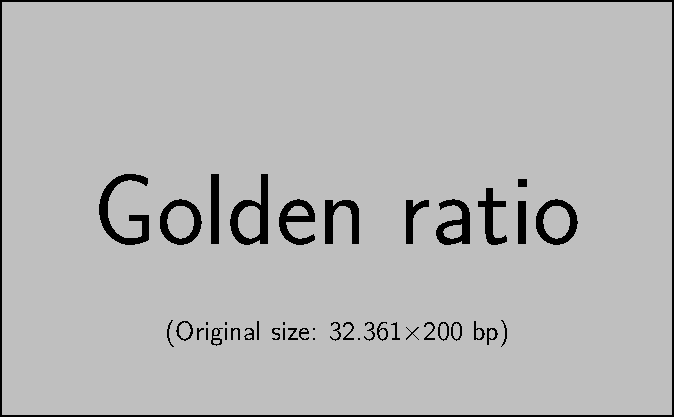
\includegraphics[width=\textwidth]{placeholder_images/example-image-golden.pdf}
    \caption[]
    {Electrolyte conductivity as a function of equilibrium concentration at
    $T_\text{cell} = \SI{298.15}{\kelvin}$}
    \label{fig:kappavsce}
\end{figure}

From~\cref{fig:kappavsce},  it  is  evident that  the  electrolyte  conductivity
attains its maximum value at $c_\text{e} = \SI{1000}{\mole\per\meter\cubed}$. It
is advantageous  to operate  the cell  around this salt  concentration so  as to
minimise  the  cell's  overall  resistance.  Hence,  the  initial  concentration
$c_\text{e,0}$ is  chosen to  be \SI{1000}{\mole\per\meter\cubed}. It  should be
noted that while  the electrolyte concentration in the  \gls{p2d} model exhibits
both spatial  and temporal  variations during the  simulation, in  the \gls{spm}
model, it remains constant throughout.

The      reduction      in      parametrisation      requirements      discussed
in~\cref{subsec:spmp2dparametrisation}    is   only    one   of    the   factors
contributing  to   the  simplicity   and  ease   of  simulation.   As  discussed
in~\cref{subsec:basicspmgeometry},   an   important  computational   requirement
that   is  present   in   the  \gls{p2d}   model,   but  completely   eliminated
from  the   \gls{spm}  is  the   requirement  of  discretisation.   As  reported
in~\cref{tbl:lcoSimParamsSPMp2d},  with  15 nodes  per  region  along the  axial
direction  and  with 10  shells  per  electrode  in  the radial  direction,  the
\gls{p2d}  model under  simulation  achieves mesh  independence  to a  tolerance
of  \approx   \SI{2}{\percent}  for  the   range  of  C-rates   considered.  For
higher  C-rates,  coupling  a  thermal   model  is  of  higher  importance  than
incorporating further meshing refinements. The discretisation-related parameters
are  specific to  the  \gls{p2d}  model and  is  hence, highlighted  accordingly
in~\cref{tbl:lcoSimParamsSPMp2d}.

With  the cell  parametrisation discussed  and the  simulation setup  presented,
the  simulation   results  are  fully   reproducible  and  are   presented  next
in~\cref{subsec:simresultsbasicspm}.

\subsection{Simulation Results}\label{subsec:simresultsbasicspm}

% electrolyte resistance
